%% ----------------------------------------------------------------
%% Thesis.tex
%% ---------------------------------------------------------------- 

\documentclass[draft]{ecsthesis}      % Use the Thesis Style
%\documentclass{ecsthesis}      % Use the Thesis Style

%\graphicspath{{../Figures/}}   % Location of your graphics files
\usepackage{natbib}            % Use Natbib style for the refs.
\usepackage{psfrag}
\usepackage{multirow}


%\linespread{0.98}


\hypersetup{colorlinks=true}   % Set to false for black/white printing
%% ----------------------------------------------------------------
%% Definitions.tex
%% ---------------------------------------------------------------- 
\newcommand{\BibTeX}{{\rm B\kern-.05em{\sc i\kern-.025em b}\kern-.08em T\kern-.1667em\lower.7ex\hbox{E}\kern-.125emX}}

%% People
%\newcounter{address}
%\setcounter{address}{1}
%\renewcommand{\theaddress}{\textsuperscript{\fnsymbol{address}}}
%\newcommand{\address}[1]{\refstepcounter{address}\theaddress#1\\}
%\newcommand{\Name}[3]{\texorpdfstring{\href{mailto:#3}{#2}#1}{#2}\xspace}
%\newcommand{\SteveRGunn}[1]{\Name{#1}{Steve R. Gunn}{S.R.Gunn@ecs.soton.ac.uk}}





\newcommand{\vide}[1]{}  % tikz drougui
\usepackage{pgfplots}  % ocrf nico gridplot


% change margins locally:
\usepackage{setspace}
\renewcommand{\baselinestretch}{1.0}



\usepackage{times}
\usepackage[utf8]{inputenc} % pour les accents
%\usepackage{euler}
\usepackage{amsmath}
\usepackage{amssymb}
\usepackage{dsfont}
\usepackage{caption} %pour figure caption in minipage which does not allow envir figure
\usepackage{float}
\usepackage{amsthm}
\usepackage{natbib}
\usepackage{tikz}
\usetikzlibrary{decorations.pathreplacing}
\usepackage{graphicx}
%\usepackage{arydshln}  % for dashed lines in table
\usepackage{algorithm}
\usepackage{algorithmic}

\usepackage{xcolor}
\definecolor{mygreen}{rgb}{0,0.6,0}
%\definecolor{mygray}{rgb}{0.5,0.5,0.5}
%\definecolor{mymauve}{rgb}{0.58,0,0.82}
%\definecolor{rulecolor}{rgb}{0.80,0.80,0.80}
%\definecolor{bgcolor}{rgb}{1.0,1.0,1.0}
\definecolor{myblue}{rgb}{0.95, 0.95, 1.}
%\definecolor{myblue}{blue1}{0.98}

%%%%%%%%%%%%%%%% code snippet %%%%%%%%%%%%%%%%%%%%%%
\usepackage{mdframed} % useful when the code is longer than 1 page

\usepackage{minted}
\definecolor{lightgray}{gray}{.98}
\newminted{python}{fontfamily=courier, fontsize=\footnotesize, bgcolor=lightgray}
%%%%%%%%%%%%%%%%%%%%%%%%%%%%%%%%%%%%%%%%%%%%%

% \usepackage{wrapfig}
% \usepackage{booktabs}
% \usepackage{amscd}
% \usepackage{latexsym}
% \usepackage{enumerate}
% \usepackage{soul}
% \usepackage{amsfonts}
\usepackage[normalem]{ulem}

% \newtheorem{definition}{Definition}
% \newtheorem{theorem}{Theorem}
% \newtheorem{corollary}{Corollary}
% \newtheorem{proposition}{Proposition}
% \newtheorem{lemma}{Lemma}
% \newtheorem{remark}{Remark}
% \numberwithin{equation}{section}
\newtheorem{notation}{\textbf{Notation}}

%\newtheorem{algorithm}{Algorithm}
\newtheorem{assumption}{Assumption}


\newcommand{\ie}{\emph{i.e.}{}}
\newcommand{\st}{\emph{s.t.}{}}
\newcommand{\eg}{\emph{e.g.}{}}
\newcommand\iid{\ensuremath{\mathit{i.i.d.}}\ }
\newcommand{\rv}{\emph{r.v.}{}}
\newcommand{\wrt}{\emph{w.r.t.}{}}
\newcommand{\cdf}{\emph{c.d.f.}{}}

\newcommand{\red}{\color{red} }
\newcommand\blue{\color{blue} }
\newcommand\green{\color{mygreen} }
% \newcommand{\tsf}{\texttt}
\newcommand{\ninf}[1]{\| {#1}\|_{\infty}}
\newcommand{\ud}{\mathrm{d}}
\newcommand{\dd}{\{1,\ldots,d\}}
\newcommand{\crit}{\mathcal{C}}
\newcommand{\hatmass}{\widehat{\mathcal{M}}}
%\renewcommand{\hatmass(\alpha)}{\widehat{M}(\alpha)}


\def\bb{\mathbb}
\def\mb{\mathbf}
\def\point{\,\cdot\,}
\def\P{\mathbb{P}}
\def\PP{\P}
\def\E{\mathbb{E}}
\def\EE{\E}
\def\rset{\mathbb{R}}
\def\nset{\mathbb{N}}
\def\cone{\mathcal{C}}
% \def\EM{{\sc EM}}
% \def\MV{{\sc MV}}
\def\stdf{{\sc stdf}}
\def\S{\mathcal{S}}
\def\xset{\mathcal{X}}
\def\crit{\mathcal{C}}
\def\roc{\textsc{ROC}}
\def\leb{\text{Leb}}
\def\Var{\mathbf{Var}}



\def\argmin{\operatornamewithlimits{arg\,min}}
\def\argmax{\operatornamewithlimits{arg\,max}}
\def\supess{\operatornamewithlimits{ess\,sup}}

%\newcommand{\argmax}{\mathop{\mathrm{arg\,max}}}











%% Dingbats
\newcommand{\tick}{\ding{51}}
\newcommand{\cross}{\ding{55}}

%% Calculus
\newcommand{\pd}[2]{\ensuremath{\frac{\partial #1}{\partial #2}}\xspace}
\newcommand{\fd}[2]{\ensuremath{\frac{d #1}{d #2}}\xspace}
\newcommand{\dint}{\ensuremath{\int\!\!\!\int}\xspace}
\newcommand{\tint}{\ensuremath{\int\!\!\!\int\!\!\!\int}\xspace}

%% Math Sets
\newcommand{\Q}[1]{\ensuremath{\mathbb{#1}}\xspace}
\newcommand{\R}{\Q{R}}

%% Matrix, Vector
\newcommand{\V}[1]{\ensuremath{\boldsymbol{#1}}\xspace}
\newcommand{\M}[1]{\ensuremath{\boldsymbol{#1}}\xspace}
\newcommand{\0}{\V{0}}
\newcommand{\1}{\V{1}}
\newcommand{\I}{\M{I}}

%% Math Functions
\newcommand{\F}[1]{\ensuremath{\mathrm{#1}}\xspace}
\newcommand{\sgn}{\F{sgn}}
\newcommand{\tr}{\F{trace}}
\newcommand{\diag}{\F{diag}}

%% Math Names
\newcommand{\N}[1]{\ensuremath{\mathit{#1}}\xspace}

%% Data
\newcommand{\mc}[1]{\ensuremath{\mathcal{#1}}\xspace}
\newcommand{\Hyp}{\mc{H}}
\newcommand{\D}{\mc{D}}

%% Kernel
\newcommand{\K}{\M{K}}
\newcommand{\eins}{\texorpdfstring{\ensuremath{\epsilon}}{\textepsilon}-insensitive\xspace}
\newcommand{\e}{\ensuremath{\epsilon}\xspace}
\newcommand{\Bxi}{\ensuremath{\boldsymbol{\xi}}\xspace}
\newcommand{\Kanova}{\ensuremath{\mathit{K_{ANOVA}}}\xspace}
\newcommand{\Kspline}{\ensuremath{\mathit{K_{spline}}}\xspace}

%% Bayesian
\newcommand{\MP}{\ensuremath{\mathit{{\scriptscriptstyle \hspace{-1.5pt}M\hspace{-1.5pt}P}}}\xspace}
\newcommand{\ML}{\ensuremath{\mathit{{\scriptscriptstyle \hspace{-1.5pt}M\hspace{-1.5pt}L}}}\xspace}
\newcommand{\Qw}{\ensuremath{Q_{\w}(\w)}\xspace}
\newcommand{\Qa}{\ensuremath{Q_{\Ba}(\Ba)}\xspace}
\newcommand{\Qb}{\ensuremath{Q_{\beta}(\beta)}\xspace}
\newcommand{\wMPab}{\ensuremath{\w_{\MP|\bar {\Ba},\bar \beta}}\xspace}
\newcommand{\wMP}{\ensuremath{\w_{\MP}}\xspace}
\newcommand{\yMP}{\ensuremath{y_{\MP}}\xspace}
\newcommand{\BaMP}{\ensuremath{\Ba_{\hspace{1pt}\MP}}\xspace}
\newcommand{\aMP}{\ensuremath{\alpha_{\hspace{1pt}\MP}}\xspace}
\newcommand{\bMP}{\ensuremath{\beta_{\hspace{1pt}\MP}}\xspace}
\newcommand{\Sab}{\ensuremath{\M{\Sigma}_{\bar \Ba,\bar \beta}}\xspace}
\newcommand{\Ba}{\ensuremath{\boldsymbol{\alpha}}\xspace}
\newcommand{\Bb}{\ensuremath{\boldsymbol{\beta}}\xspace}
\newcommand{\Bm}{\ensuremath{\boldsymbol{\mu}}\xspace}
\newcommand{\BL}{\ensuremath{\boldsymbol{\Lambda}}\xspace}
\newcommand{\BPhi}{\ensuremath{\boldsymbol{\Phi}}\xspace}
\newcommand{\SMP}{\ensuremath{\M{\Sigma}_{\MP}}\xspace}

\newcommand{\Pa}{\ensuremath{P(\alpha|\mathcal{H})}\xspace}
\newcommand{\Pb}{\ensuremath{P(\beta|\mathcal{H})}\xspace}
\newcommand{\Pab}{\ensuremath{P(\alpha,\beta|\mathcal{H})}\xspace}
\newcommand{\Pw}{\ensuremath{P(\w|\mathcal{H})}\xspace}
\newcommand{\PD}{\ensuremath{P(\D|\mathcal{H})}\xspace}
\newcommand{\PwIa}{\ensuremath{P(\w|\alpha,\mathcal{H})}\xspace}
\newcommand{\PDIwb}{\ensuremath{P(\D|\w,\beta,\mathcal{H})}\xspace}
\newcommand{\PDwab}{\ensuremath{P(\D,\w,\alpha,\beta|\mathcal{H})}\xspace}
\newcommand{\PDIw}{\ensuremath{P(\D|\w,\mathcal{H})}\xspace}
\newcommand{\PwID}{\ensuremath{P(\w|\D,\mathcal{H})}\xspace}
\newcommand{\PwabID}{\ensuremath{P(\w,\alpha,\beta|\D,\mathcal{H})}\xspace}

\newcommand{\PanH}{\ensuremath{P(\alpha)}\xspace}
\newcommand{\PbnH}{\ensuremath{P(\beta)}\xspace}
\newcommand{\PabnH}{\ensuremath{P(\alpha,\beta)}\xspace}
\newcommand{\PwnH}{\ensuremath{P(\w)}\xspace}
\newcommand{\PDnH}{\ensuremath{P(\D)}\xspace}
\newcommand{\PwIanH}{\ensuremath{P(\w|\alpha)}\xspace}
\newcommand{\PDIwbnH}{\ensuremath{P(\D|\w,\beta)}\xspace}
\newcommand{\PDwabnH}{\ensuremath{P(\D,\w,\Ba,\beta)}\xspace}
\newcommand{\PDIwnH}{\ensuremath{P(\D|\w)}\xspace}
\newcommand{\PwIDnH}{\ensuremath{P(\w|\D)}\xspace}
\newcommand{\PwabIDnH}{\ensuremath{P(\w,\alpha,\beta|\D)}\xspace}

\newcommand{\PDwBab}{\ensuremath{P(\D,\w,\Ba,\beta|\mathcal{H})}\xspace}
\newcommand{\PwIBa}{\ensuremath{P(\w|\Ba,\mathcal{H})}\xspace}
\newcommand{\PBab}{\ensuremath{P(\Ba,\beta|\mathcal{H})}\xspace}
\newcommand{\PwBabID}{\ensuremath{P(\w,\Ba,\beta|\D,\mathcal{H})}\xspace}

\newcommand{\PBanH}{\ensuremath{P(\Ba)}\xspace}
\newcommand{\PwIBanH}{\ensuremath{P(\w|\Ba)}\xspace}

%% Snakes
\newcommand{\Esnake}{\ensuremath{\mathit{E_{snake}}}\xspace}
\newcommand{\Eimage}{\ensuremath{\mathit{E_{image}}}\xspace}
\newcommand{\Econt}{\ensuremath{\mathit{E_{cont}}}\xspace}
\newcommand{\Ecurv}{\ensuremath{\mathit{E_{curv}}}\xspace}
\newcommand{\Eint}{\ensuremath{\mathit{E_{int}}}\xspace}
\newcommand{\Eext}{\ensuremath{\mathit{E_{ext}}}\xspace}
\newcommand{\Eterm}{\ensuremath{\mathit{E_{term}}}\xspace}
\newcommand{\Eline}{\ensuremath{\mathit{E_{line}}}\xspace}
\newcommand{\Eedge}{\ensuremath{\mathit{E_{edge}}}\xspace}
\newcommand{\Econ}{\ensuremath{\mathit{E_{con}}}\xspace}
\newcommand{\Eangle}{\ensuremath{\mathit{E_{angle}}}\xspace}
\newcommand{\Elshape}{\ensuremath{\mathit{E_{lshape}}}\xspace}
\newcommand{\Eedgedir}{\ensuremath{\mathit{E_{edgedir}}}\xspace}
\newcommand{\Emodel}{\ensuremath{\mathit{E_{model}}}\xspace}
\newcommand{\wte}{\ensuremath{\mathit{w_{term}}}\xspace}
\newcommand{\wli}{\ensuremath{\mathit{w_{line}}}\xspace}
\newcommand{\wed}{\ensuremath{\mathit{w_{edge}}}\xspace}
\newcommand{\wco}{\ensuremath{\mathit{w_{con}}}\xspace}

%% Environments
% \newcounter{alg}
% \newenvironment{algorithm}[1]
% {
%     \stepcounter{alg}
%     \begin{table}[htb]
%     \centering
%     \begin{tabular}[t]{ll}
%     \hline&\\
%     \multicolumn{2}{l}{\bf Algorithm \arabic{alg}: #1}\\&\\
% } {
%     &\\
%     \hline
%     \end{tabular}
%     \end{table}
% }
\newcommand{\innerp}[1]{\left\langle #1 \right\rangle}
\DeclareMathOperator{\rank}{rank}

% \usepackage{amsfonts}
% \newcommand{\tickYes}{\textcolor{green}{\checkmark}}
% \usepackage{pifont}
% \newcommand{\tickNo}{\textcolor{red}{\hspace{1pt}\ding{55}}}

\usepackage{epigraph}
%\setlength{\epigraphwidth}{0.7\textwidth}
%\epigraph{There is nothing more practical than a good theory}{\textit{Kurt Lewin}}

% nicer backref links
%\renewcommand*{\backref}[1]{}
%\renewcommand*{\backrefalt}[4]{%
%\ifcase #1 %
%(Not cited.)%
%\or
%(Cited on page~#2)%
%\else
%(Cited on pages~#2)%
%\fi}
%\renewcommand*{\backrefsep}{, }
%\renewcommand*{\backreftwosep}{ and~}
%\renewcommand*{\backreflastsep}{ and~}

\usepackage{gastex}

\newenvironment{proof2}[1][Proof]{\begin{trivlist}
\item[\hskip \labelsep {\bfseries #1}]}{\end{trivlist}}
\newenvironment{proof3}[1][]{\begin{trivlist}
\item[\hskip \labelsep {\bfseries #1}]}{\hfill$\Box$\end{trivlist}}

%\definecolor{gray2}{gray}{0.97}
\makeatletter\newenvironment{bc_box}{%
   \begin{lrbox}{\@tempboxa}\begin{minipage}{0.9\columnwidth}}{\end{minipage}\end{lrbox}%
   {\setlength{\fboxsep}{8pt}\colorbox{myblue}{\usebox{\@tempboxa}}}
}\makeatother
\newenvironment{chapabstract}{
  \begin{small}
  \begin{center}
  \begin{bc_box}\textbf{Abstract}
}{
  \end{bc_box}
  \end{center}
  \end{small}
}

\makeatletter\newenvironment{bc_box_abstract_end}{%
   \begin{lrbox}{\@tempboxa}\begin{minipage}{\columnwidth}}{\end{minipage}\end{lrbox}%
   {\setlength{\fboxsep}{8pt}\colorbox{myblue}{\usebox{\@tempboxa}}}
}\makeatother

\usepackage{bibentry}
\makeatletter
\let\BRatbibitem\BR@bibitem
\makeatother

\usepackage{titlesec}
\titleformat{\chapter}[display]{\Large\bfseries}{\titlerule\vspace*{-12pt}\filleft\MakeUppercase{\chaptertitlename} \Huge\thechapter\vspace*{-12pt}}{0pt}{\filleft\Large\bfseries\sffamily}[\titlerule]
%\titlespacing*{\chapter}{0pt}{50pt}{40pt}

\titleformat{\part}[frame]{\LARGE\bfseries}{\filcenter\MakeUppercase{\partname} \Huge\thepart}{30pt}{\filcenter\Huge\bfseries\sffamily}

\usepackage[all]{hypcap} % make figure/table links point at the top instead of bottom

\usepackage{booktabs} % better tables
\renewcommand{\arraystretch}{1.1}

%\DeclareMathOperator{\sign}{sign}


% % change margins pour l'abstract:
% \newenvironment{changemargin}[2]{%
% \begin{list}{}{%
% \setlength{\topsep}{0pt}%
% \setlength{\leftmargin}{#1}%
% \setlength{\rightmargin}{#2}%
% \setlength{\listparindent}{\parindent}%
% \setlength{\itemindent}{\parindent}%
% \setlength{\parsep}{\parskip}%
% }%
% \item[]}{\end{list}}
            % Include your abbreviations
%% ----------------------------------------------------------------


\setcounter{secnumdepth}{3} % seting level of numbering (default for "report" is 3). With ''-1'' you have non number also for chapters
\setcounter{tocdepth}{2}


\begin{document}
\begingroup
  \makeatletter
  \let\BR@bibitem\BRatbibitem
  \nobibliography*
\endgroup
\frontmatter
\title      {Machine Learning and Extremes for Anomaly Detection}
\titre      {Apprentissage Automatique et Extrêmes pour la Détection d'Anomalies}
\authors    {Nicolas Goix}
\date       {Octobre 2016}
\subject    {PhD Thesis}
\keywords   {Anomaly Detection, Dimensionality Reduction, Multivariate Extremes, Concentration}
\maketitle
\begin{listpublis}

\subsection*{Journal}
\begin{itemize}
\item Sparse Representation of Multivariate Extremes with Applications to Anomaly Detection. (Under review for Journal of Multivariate Analysis).\\
Authors: Goix, Sabourin, and Clémençon.
\end{itemize}

\subsection*{Conferences}
\begin{itemize}
\item On Anomaly Ranking and Excess-Mass Curves. (AISTAT 2015).\\
Authors: Goix, Sabourin, and Clémençon. 

\item Learning the dependence structure of rare events: a non-asymptotic study. (COLT 2015).\\
Authors: Goix, Sabourin, and Clémençon.

\item Sparse Representation of Multivariate Extremes with Applications to Anomaly Ranking. (AISTAT 2016).\\
Authors: Goix, Sabourin, and Clémençon.

\item How to Evaluate the Quality of Unsupervised Anomaly Detection Algorithms? (submitted).\\ Authors: Goix and Thomas. 

\item One-Class Splitting Criteria for Random Forests with Application to Anomaly Detection. (submitted).\\
Authors: Goix, Brault, Drougard and Chiapino.
\end{itemize}


\subsection*{Workshops}
\begin{itemize}
\item Sparse Representation of Multivariate Extremes with Applications to Anomaly Ranking. (NIPS 2015 Workshop on Nonparametric Methods for Large Scale Representation Learning).\\
Authors: Goix, Sabourin, and Clémençon.

\item How to Evaluate the Quality of Unsupervised Anomaly Detection Algorithms? (ICML 2016, Workshop on Anomaly Detection). Co-winner of the Best Paper Award, sponsored by Google.\\
Author: Goix. 
\end{itemize}

\subsection*{Scikit-Learn implementations}
\begin{itemize}
\item Isolation Forest: https://github.com/scikit-learn/scikit-learn/pull/4163\\
Authors: Goix and Gramfort
\item Local Outlier Factor: https://github.com/scikit-learn/scikit-learn/pull/5279\\
Authors: Goix and Gramfort
\end{itemize}

  
\end{listpublis}
\begin{acknowledgements}
  Je souhaite tout d'abord remercier mes directeurs de thèse, Stephan et Anne; la complémentarité de vos encadrements respectifs constitue un magma favorable à la recherche! En particulier, merci Stéphan pour l'originalité du sujet de thèse, pour ton recul sur la littérature, pour ta disponibilité et ta sympathie. Merci aussi pour le dynamisme apporté à l'équipe STA, qui s'est créée une réputation internationale en marquant fièrement sa présence aux grosses conférences de machine learning. Merci Anne pour ton encadrement exemplaire, je suis content d'avoir été ton premier "thésard" et d'avoir passé ces heures d'échange devant un tableau rempli d'extrêmes, merci pour ta sympathie et ta patience.

Je tiens aussi à remercier mes collègues 
de bureau, Igor Colin et Albert Thomas (on est un bureau mince!), Aurélien Bellet, Antoine Demattéo, Ruocong Zhang, 
de couloir, 

 d'étage et de batiment, à savoir 

\end{acknowledgements}


\tableofcontents
\listoffigures
\listoftables
%\lstlistoflistings
%\listofsymbols{ll}{}
%\dedicatory{To \dots}
% %% ----------------------------------------------------------------
% \thispagestyle{plain}
%
% \null\vfill
% ``There is nothing more practical than a good theory.''
%
% \begin{flushright}
% --- James C. Maxwell
% \end{flushright}
%
% \vspace*{1cm}
%
% ``There is a theory which states that if ever anyone discovers exactly what the Universe is for and why it is here, it will instantly disappear and be replaced by something even more bizarre and inexplicable.
%
% There is another theory which states that this has already happened.''
%
% \begin{flushright}
% --- Douglas Adams
% \end{flushright}
%
% \vfill\vfill\vfill\vfill\vfill\vfill\null
% \clearpage
% %% ----------------------------------------------------------------

\mainmatter
%% ----------------------------------------------------------------
\chapter{Summary}\label{chap:intro}
%%\addcontentsline{toc}{part}{\nameref{chap:intro}}
%%\counterwithout{section}{chapter}

\section{Introduction}
\emph{Anomaly}, from Greek $\alpha\nu\omega\mu\alpha\lambda\iota\alpha$, asperity, irregular, not the same (an-homalos), refers to a gap, a deviation with respect to some norm or basis, reflecting the expected behavior.
We call \emph{anomaly} the object inducing a gap, the observation which deviates from normality. 
%
In various fields, the following situation occurs: an expert aims at predicting a phenomenon based on previous observations. The most basic case is when one wants to predict some binary characteristic of some new observations/records, given previous ones. For instance one can think of a doctor aiming to predict if an incoming patient has a fixed pathology or not, using previous patients record (such as age, history, gender, blood pressure) associated with their true \textbf{label} (having the pathology or not). This case is an example of \emph{binary classification}, where the doctor aims to find a rule to \textbf{predict} the label of a new patient (the latter being characterized by its record). This rule is called a \emph{classifier} and it has to be built, or \emph{trained}, on previous records. % (namely records associated with their labels). 
Intuitively, the classifier will predict the same diagnosis for similar records, in a sense that should be learned accurately.

Two cases can be distinguished. If labels of previous patients are known/available, \ie~previous patients are known to be sick or healthy: the classification task is said to be \textbf{supervised}. If training labels are unknown, the classification is said \textbf{unsupervised}. Following our example, the doctor has to find two patterns (or clusters), healthy/sick, each containing similar patient records.

Anomaly detection occurs when one label is highly under-represented for training, for instance if very few patients have the pathology in the training database.
Thus, \textbf{supervised anomaly detection} boils down to \emph{rare class mining}, namely supervised classification on highly unbalanced classes. 
As to \textbf{unsupervised anomaly detection} (also simply called outlier detection), it generally assumes that the database has a hidden `normal' model, and anomalies are observations which deviate from this model. The doctor wants to find records which deviate from the vast majority of those of his previous patients. 
%
His task is in some way simplified if he knows all of its previous patients to be healthy: it is easier for him to learn the `normal' model, \ie~the typical record of a healthy patient, to be confronted with new records. This is the so-called \textbf{novelty detection} framework (also called one-class classification or semi-supervised anomaly detection), where the training database only contains normal instances. 

This chapter is organized as follows.
First in Section~\ref{resume:scoring_function}, the anomaly detection task is formally introduced as well as the concept of scoring function. 
Two criteria for `being a good scoring function' are presented in Section \ref{resume:scoring}, allowing an M-estimation approach. 
Section~\ref{resume:extreme} focuses on extreme value theory (EVT) to gain in accuracy on extreme regions. It introduces the \emph{stable tail dependence function} (STDF), to estimate the dependence structure of rare events (Section~\ref{resume:stdf}) and shows that multivariate EVT can be useful to produce scoring functions accurate on low probability regions (Section~\ref{resume:sec:JMVA}).
Section~\ref{resume:sec:heuristic} gathers two contributions to be submitted addressing the evaluation of unsupervised anomaly detection from a practical point of view (Section~\ref{resume:evaluation}), and the extension of random forests to the one-class setting (Section~\ref{resume:ocrf}). Section~\ref{sec:impl} presents contributions relative to a widely used open-source machine learning library. Section~\ref{intro:concl} details the scientific output and concludes.



%Each patient record $i$ being a set of measurements may be summarized into a $d$-dimensional vector $\mb X_i$, and its label into a binary value $y_i \in \{0, 1\}$ (healthy, sick). The set of all training labeled record $(\mb X_1, y_1),\ldots, (\mb X_d, y_d)$ from patients $1, \ldots, d$ form the so-called \textbf{training database}. 
\paragraph{Notations}

Throughout this document, $\mathbb{N}$ denotes the set of natural numbers while $\mathbb{R}$ and $\mathbb{R}_+$ respectively denote the sets of real numbers and non-negative real numbers. Arbitrary sets are denoted by calligraphic letters such as $\mathcal{G}$, and $|\mathcal{G}|$ stands for the number of elements in $\mathcal{G}$. % A set of $m$ elements from $\mathcal{G}$ is denoted by $\mathcal{G}^m$.
%
We denote vectors by bold lower case letters. For a vector $\mathbf{x}\in\mathbb{R}^d$ and $i\in \{1,\dots,d\}$, $x_i$ denotes the $i^{th}$ component of $\mathbf{x}$. The inner product between two vectors is denoted by $\innerp{\cdot,\cdot}$. $\|\cdot\|$ denotes an arbitrary (vector or matrix) norm and $\|\cdot\|_p$ the $L_p$ norm.
%
%We denote matrices by bold upper case letters. For a $c\times d$ real-valued matrix $\mathbf{M}\in\mathbb{R}^{c\times d}$ and a pair of integers $(i,j)\in[c]\times[d]$, $M_{i,j}$ denotes the entry at row $i$ and column $j$ of the matrix $\mathbf{M}$. The identity matrix is denoted by $\mathbf{I}$ and the cone of symmetric positive semi-definite (PSD) $d\times d$ real-valued matrices by $\mathbb{S}^{d}_+$. 
%Strings are denoted by sans serif letters such as $\mathsf{x}$. We use $|\mathsf{x}|$ to denote the length of $\mathsf{x}$ and $\mathsf{x_i}$ to refer to its $i^{th}$ symbol.
%
%In the context of learning problems, we use $\mathcal{X}$ and $\mathcal{Y}$ to denote the input space (or instance space) and the output space (or label space) respectively. We use $\mathcal{Z}=\mathcal{X}\times\mathcal{Y}$ to denote the joint space, and an arbitrary labeled instance is denoted by $z=(x,y)\in\mathcal{Z}$. The hinge function $[\cdot]_+:\mathbb{R}\to\mathbb{R}_+$ is defined as $[c]_+=\max(0,c)$. 
%
Throughout this thesis, $\PP[A]$ denotes the probability of the event $A\in \Omega$, the underlying probability space being $(\Omega, \mathcal{F}, \PP)$. We denote by $\mathbb{E}[X]$ the expectation of the random variable $X$. $X \overset{d}{=} Y$ means that $X$ and $Y$ are equal in distribution and $X_n \overset{d}{\to} Y$ means that $(X_n)$ converges to $Y$ in distribution. We often use the abbreviation $\mb X_{1:n}$ to denote an \iid~sample $(\mb X_1,\ldots,\mb X_n)$.
%
%$x\sim P$ indicates that $x$ is drawn according to the probability distribution $P$.
%
A summary of the notations is given in \tref{tab:notations}.

\begin{table}[!ht]
\begin{center}
\begin{footnotesize}
\begin{tabular}{lp{1cm}l}
\toprule
\textbf{Notation} && \textbf{Description}\\
\midrule
$\cdf$ && cumulative distribution function\\
$\rv$ && random variable\\
$\mathbb{R}$ && Set of real numbers\\
$\mathbb{R}_+$ && Set of nonnegative real numbers\\
$\mathbb{R}^d$ && Set of $d$-dimensional real-valued vectors\\
$\leb(\cdot)$ && Lebesgue measure on $\mathbb{R}$ or $\mathbb{R}^d$\\
$(\cdot)_+$ && positive part\\
$\vee$ && maximum operator\\
$\wedge$ && minimum operator\\
%$\mathbb{R}^{c\times d}$ && Set of $c\times d$ real-valued matrices\\
$\mathbb{N}$ && Set of natural numbers, i.e., $\{0,1,\dots\}$\\
%$\mathbb{S}^{d}_+$ && Cone of symmetric PSD $d\times d$ real-valued matrices\\
%$[k]$ && The set $\{1,2,\dots,k\}$\\
$\mathcal{G}$ && An arbitrary set\\
$|\mathcal{G}|$ && Number of elements in $\mathcal{G}$\\
%$\mathcal{G}^m$ && A set of $m$ elements from $\mathcal{S}$\\
%$\mathcal{X}$ && Input space\\
%$\mathcal{Y}$ && Output space\\
%$z=(x,y)\in\mathcal{X}\times\mathcal{Y}$ && An arbitrary labeled instance\\
$\mathbf{x}$ && An arbitrary vector\\
$\mb x < \mb y$ && component-wise vector comparison\\
$\mb m$ (for $m \in \rset$) && vector $(m,\ldots,m)$\\
$\mb x < m$ && means $\mb x < \mb m$\\
$x_j$ && The $j^{th}$ component of $\mathbf{x}$\\
$\delta_{\mb a}$ && Dirac mass at point $a \in \mathbb{R}^d$\\
$\lfloor \cdot \rfloor$ && integer part\\
$\innerp{\cdot,\cdot}$ && Inner product between vectors\\
%$[\cdot]_+$ && Hinge function\\
%$\mathbf{M}$ && An arbitrary matrix\\
%$\mathbf{I}$ && The identity matrix\\
%$M_{i,j}$ && Entry at row $i$ and column $j$ of matrix $\mathbf{M}$\\
$\|\cdot\|$ && An arbitrary norm\\
$\|\cdot\|_p$ && $L_p$ norm\\
%$\mathsf{x}$ && An arbitrary string\\
%$|\mathsf{x}|$ && Length of string $\mathsf{x}$\\
%$\mathsf{x_i},\mathsf{x_{i,j}}$ && $j^{th}$ symbol of $\mathsf{x}$ and $\mathsf{x_i}$\\
%$x\sim P$ && $x$ is drawn i.i.d. from probability distribution $P$\\
$A\Delta B$ && symmetric difference between sets $A$ and $B$ \\
$(\Omega, \mathcal{F}, \PP)$ && Underlying probability space\\
$\mathcal{S}$ && functions $s: \mathbb{R}^d \rightarrow \mathbb{R}_+ $ integrable \wrt~ Lebesgue measure (scoring functions)\\
$\overset{d}{\to}$ && Weak convergence of probability measures or \rv\\
$\mathbf{X}$ && A \rv~with values in $\mathbb{R}^d$\\
$\mathds{1}_{\mathcal{E}}$ && indicator function event $\mathcal{E}$\\
$Y_{(1)} \le \ldots\le Y_{(n)}$ && order statistics of $Y_1,\ldots,Y_n$\\
$\mb X_{1:n}$ && An \iid~sample $(\mb X_1,\ldots,\mb X_n)$\\
$\PP[\cdot]$ && Probability of event\\
$\EE[\cdot]$ && Expectation of random variable\\
$\Var[\cdot]$ && Variance of random variable\\

\bottomrule
\end{tabular}
\end{footnotesize}
\caption[Summary of notation]{Summary of notation.}
\label{tab:notations}
\end{center}
\end{table}


\section{Anomaly Detection, Anomaly Ranking and Scoring Functions}
\label{resume:scoring_function}
From a probabilistic point of view, there are different ways of modeling normal and abnormal behaviors, which leads to different methodologies. One natural probabilistic model is to assume two different generating processes for normal and abnormal data. Normal data (resp. abnormal data) are generated according to some distribution $F$ (resp. $G$). The general underlying distribution is then a mixture of $F$ and $G$. The goal is to find out whether a new observation $\mb x$ has been generated from $F$, or from $G$. The optimal way to resolve theoretically this problem is the likelihood ratio test, also called Neyman-Pearson test. If $(\ud  F / \ud  G) ( \mb x) > t$ with some $t>0$ threshold, then $\mb x$ has been drawn from $F$. Otherwise, $\mb x$ has been drawn from $G$. This boils down to estimating the \emph{density level set} $\{\mb x, (\ud F / \ud  G) (\mb x) > t\}$ \citep{Scholkopf2001, Steinwart2005, Scott2006, VertVert}.
%
As anomalies are very rare, their structure cannot be observed in the data, in particular their distribution $G$. 
%
It is common and convenient to replace $G$ in the problem above by the Lebesgue measure, so that it boils down to estimating density level set of $F$
\citep{Scholkopf2001, Scott2006, VertVert}.

This comes back to assume that anomalies are uniformly distributed on the support of the normal distribution. %\citep{Steinwart2005, Blanchard2010}. 
This assumption is thus implicitly made by a majority of works on novelty detection.
 % This simplifying choice corresponds to making the assumption either that anomalies are uniformly distributed, or that no anomaly is observed during training. In other words, this modeling choice applies to novelty detection.
We observe data in $\rset^d$ from the normal class only, with an underlying distribution $F$ and with a density $f: \rset^d \to \rset$. 
%Abnormal data are assumed to be in the tail of $F$.
The goal is to identify characteristics of this normal class, such as its support $\{\mb x, f( \mb x) > 0\}$ or some density level set $\{\mb x, f( \mb x) > t\}$ with $t>0$ close to $0$.

This \emph{one-class classification} problem is different than \emph{distinguishing} between several classes as done in standard classification. Also, unsupervised anomaly detection is often viewed as a one-class classification problem, where training data are polluted by a few elements of the abnormal class: it appeals for one-class algorithms \emph{robust to anomalies}. 

%This way of modeling appeals for \emph{density level set estimation} analysis.

A natural idea for estimating density level sets is to compute an estimate of the density and to consider the associated plug-in density level sets \citep{Tsybakov1997, Cuevas1997, Baillo2001, Baillo2003, Cadre2006, Rigollet2009, Mason2009}.
The density is generally estimated using non-parametric kernel estimator or maximum likelihood estimator from some parametric family of functions. But these methods does not scale well with the dimension. They try somehow to capture more information than needed for the level set estimation task, such as local properties of the density which are useless here. Indeed, it turns out that for any increasing transform $T$, the level sets of $T\circ f$ are exactly those of $f$. Thus, it suffices to estimate any representative of the class of all increasing transforms of $f$, to obtain density level sets estimates. Intuitively, it is enough to estimate the pre-order (the \emph{scoring}) induced by $f$ on $\rset^d$. Let us define a \emph{scoring function} as any measurable function $s:~\rset^d \to \rset_+$ integrable \wrt~the Lebesgue measure $\leb(.)$, and $\S$ the space of all scoring functions.
Any scoring function defines a pre-order on $\rset^d$ and thus a ranking on a set of new observations. This ranking can be interpreted as a degree of abnormality, the lower $s(x)$, the more abnormal $x$. Note incidentally that most anomaly detection algorithms return more than a binary label, normal/abnormal. They return a scoring function, which can be converted to a binary prediction, typically by imposing some threshold based on its statistical distribution.

Suppose we are interested in learning a scoring function $s$ whose induced pre-order is `close' to that of $f$, or equivalently whose induced level sets are close to those of $f$. The problem is to turn this notion of proximity into a criterion $\crit$, optimal scoring functions $s^*$ being then defined as those optimizing $\crit$. In the density estimation framework, the uniform difference $\|f - \hat f\|_\infty$ is a common criterion to assess the quality of the estimation. We would like a similar criterion but which is invariant by increasing transformation of the output $\hat f$. In other words, the criterion should be defined such that the collection of level sets of an optimal scoring function $s^*(x)$ coincides with that related to $f$, and any increasing transform of the density should be optimal regarding $\crit$.
More formally, we are going to consider $\crit^{\Phi}(s) = \| \Phi(s) - \Phi(f) \|$ (instead of $\|s - f\|$) % for the Mass-Volume criterion (resp. $ \|EM_s - EM_f\|$ for the Excess-Mass criterion),
with $\Phi: \mathbb{R} \to \mathbb{R}_+$ verifying $\Phi(T \circ s) = \Phi(s)$ 
% (resp. $EM_{T \circ s} = EM_s$)
for any scoring function $s$ and increasing transform $T$. Here $\Phi(s)$ denotes either the mass-volume curve $MV_s$ of $s$ or its excess-mass curve $EM_s$, which are defined in the next section.  



This criterion which measures the quality of a scoring function is then a tool for building/learning a good scoring function.
According to the Empirical Risk Minimization (ERM) paradigm, a scoring function is built by optimizing  an empirical version $\crit_n(s)$ of the criterion over an adequate set of scoring functions $\S_0$ of controlled complexity (\textit{e.g.} a class of finite {\sc VC} dimension). %Hence, another desirable property to guarantee the universal consistency of ERM learning strategies is the uniform convergence of $\crit_n(s)$ to $\crit(s)$ over such collections $\S_0$ under minimal assumptions on the distribution $F$.

The next section describes two criteria, which are functional due to the global nature of the problem just like the \emph{Receiver Operating Characteristic} (\roc) and \emph{Precision-Recall} (PR) curves, and which are admissible with respect to the requirements listed above. These functional criteria extend somehow the concept of $\roc$ curve to the unsupervised setup.

\begin{remark}{\bf Terminology: anomaly detection, anomaly ranking.\\}
Strictly speaking, criteria we are looking for are anomaly \emph{ranking} criteria, in the same way the ROC curve is basically a criterion for bipartite \emph{ranking}.
%
In practice as mentioned above, all the algorithms dealing with anomalies are candidates for the anomaly ranking task. They all produce a ranking/scoring function, even the ones which originally deal with the `anomaly classification' framework, % a single one-class classification problem,
\ie~seek to be optimal on a single level set or \wrt~a fixed false positive rate.
% ON NE PEUT PAS DEFINIR UNE SOUS CATEGORIE d'algo PAR UN BUT INITIAL: IL FAUT LA DEFINIR SUIVANT CE QU'Elle PRODUIt
% OU: LE BUT INITIAL ETANT RANKING, ON PEUT PRETENDRE QUE LE RANKING PRODUIT PAR CLASSIF A UN CERTAIN NIVEAU EST UN BON CANDIDAT.
In the literature, the `anomaly detection' terminology is widely used, instead of the more precise `anomaly ranking' one. For instance, \cite{Liu2008} write `\emph{The task of anomaly detection is to provide a ranking that reflects the degree of anomaly}'.
%
% Strictly speaking, anomaly detection should includes both anomaly ranking and anomaly classification.
In this work, we similarly make the convention that anomaly detection refers to anomaly ranking: if labels are available for the evaluation step, the goal is to maximize the area under the ROC curve. If no labeled data is available, the goal is to maximize the alternative criteria defined in the next section.

%We also abusively use the term \emph{one-class classification} to denote what should be properly called \emph{one-class ranking}, namely the anomaly ranking framework when the training data are not polluted by outliers, also called \emph{novelty detection}.

% Strictly speaking, we should speak about \emph{anomaly ranking} instead of anomaly detection. Indeed, all classical anomaly detection algorithms return first a \emph{ranking (or scoring) function} which ranks the observations according to their supposed degree of abnormality, and which can be thresholded to produce a binary label, normal vs. abnormal. Besides, all of them also evaluate themselves in terms of area under the ROC curve (when some labeled data are available to compute the latter) over some specific interval (not over a single point).

% Strictly speaking, anomaly detection focuses on some fixed $t$-level set (or on some fixed false positive rate), while anomaly ranking consider an infinite number of such one-class classification problem to rank the observations according to their supposed degree of abnormality. 
% In practice, the overwhelming majority of classical algorithms dealing with anomalies are able to rank anomalies: All of them compute first a \emph{ranking (or scoring) function} which can be thresholded to produce a binary label, normal vs. abnormal.

% In other words, in terms of output there is in practice no difference between anomaly detection or anomaly ranking.
% There could be a difference in terms of performance evaluation. When labels are available, anomaly detection algorithms should aim at maximizing a fixed point in the ROC curve, while anomaly ranking ones should aim at maximizing the curve over an interval.

% But again, in practice, all algorithms evaluate themselves in terms of area under the ROC curve (when some labeled data are available to compute the latter) over some specific interval, \ie~in term of ranking algorithms.

% Then, the only difference should be in terms of methodology or problem formulation.
% But lots of algorithms calling themselves anomaly detectors do not try to optimize any criterion
%%%%%%%%%%%%%%%%%%

\end{remark}


\section{M-estimation and criteria for scoring functions}
\label{resume:scoring}
% ou: DLSE-based Criterion to build and evaluate scoring functions

% In \cite{CLEM13,CLEM14}, a functional criterion referred to as the Mass-Volume ($MV$) curve, admissible with respect to the requirements listed above has been introduced, extending somehow the concept of $\roc$ curve in the unsupervised setup. Relying on the theory of \textit{minimum volume} sets (see \textit{e.g.} \cite{Polonik97,ScottNowak06} and the references therein), it has been proved that the scoring functions minimizing empirical and discretized versions of the $MV$ curve criterion are accurate when the underlying distribution has compact support and a first algorithm for building nearly optimal scoring functions, based on the estimate of a finite collection of properly chosen minimum volume sets, has been introduced and analyzed. However, by construction, learning rate bounds are rather slow (of the order $n^{-1/4}$ namely) and cannot be established in the unbounded support situation, unless very restrictive assumptions are made on the tail behavior of $F(dx)$. See Figure \ref{algo-problem} and related comments for an insight into the gain resulting from the concept introduced in the present paper in contrast to the $MV$ curve minimization approach. 
This section is a summary of Chapter~\ref{aistat:chap}, which is based on previous work published in \cite{AISTAT15}. We provide a brief overview of the mass-volume curve criterion introduced in \cite{CLEM13}, which is based on the notion of minimum volume sets. We then exhibit the main drawbacks of this approach, and propose an alternative criterion, the excess-mass curve to circumscribe these drawbacks. 

\subsection{Minimum Volume sets}
\label{resume:mv-set}
The notion of minimum volume set (\cite{Polonik97, Einmahl1992}) has been introduced to describe regions where a multivariate \rv~$\mb X \in \rset^d$ takes its values with highest/smallest probability.  Let $\alpha\in (0,1)$, a minimum volume set $\Gamma^*_{\alpha}$ of mass at least $\alpha$ is any solution of the constrained minimization problem
\begin{equation}\label{eq:MV}\min_{\Gamma~ \text{borelian}} ~\leb(\Gamma) \mbox{~subject to~} \mathbb{P}(\mb X \in \Gamma) \ge \alpha,
\end{equation}
where the minimum is taken over all measurable subsets $\Gamma$ of $\rset^d$.
It can be shown that every density level set is a minimum volume set for a specific mass target, and that the reverse is true if the density has no flat part. % (in fact, if a slightly stronger assumption holds, namely that the density has $\gamma$-exponent, see~\cite{Vert06thesis} for instance).
%
In the remaining of this section we suppose that $F$ has a density $f(x)$ \wrt~the Lebesgue measure on $\rset^d$ satisfying the following assumptions:

\noindent $\mathbf{A_1}$ {\it The density $f$ is bounded.}%, \textit{i.e.} $\vert \vert f(\mb X)\vert\vert_{\infty}<+\infty~.$}

\noindent $\mathbf{A_2}$ {\it The density $f$ has no flat parts: $\forall c\geq 0$, $\mathbb{P}\{f(\mb X)=c\}=0~.$}

% Application of this concept includes in particular novelty/anomaly detection: for large values of $\alpha$, abnormal observations are those which belong to the complementary set $X\setminus\Omega^*_{\alpha}$
%  for each $\alpha \in (0,1)$ there exists a threshold value $t^*_{\alpha}$
% % \overset{def}{=}Q(f, \alpha)\geq 0
%  such that $\Omega^*_{\alpha}= \{ \mb x,f( \mb x) \ge t^*_{\alpha} \}$.
Under the hypotheses above, for any $\alpha\in (0,1)$, there exists a unique minimum volume set $\Gamma_\alpha^*$, whose mass is equal to $\alpha$ exactly.
The (generalized) quantile function is then defined by:
$$
\forall \alpha\in (0,1),\;\; \lambda^*(\alpha) := \leb(\Gamma^*_{\alpha}).
$$
Additionally, the mapping $\lambda^*$ is continuous on $(0,1)$ and uniformly continuous on $[0,1-\epsilon]$ for all $\epsilon \in (0,1)$ -- when the support of $F$ is compact, uniform continuity holds on the whole interval $[0,1]$.


Estimates $\widehat{\Gamma}^*_{\alpha}$ of minimum volume sets are built by replacing the unknown probability distribution $F$ by its empirical version $F_n=(1/n)\sum_{i=1}^n\delta_{\mb X_i}$ and restricting optimization to a collection $\mathcal{A}$ of borelian subsets of $\rset^d$.  $\mathcal{A}$ is  assumed to be rich enough to include all density level sets, or at least reasonable approximates of the latter. 
In \cite{Polonik97}, limit results are derived for the generalized empirical quantile process $\{\leb(\widehat{\Gamma}^*_{\alpha})-\lambda^*(\alpha)\}$ (under the assumption in particular that $\mathcal{A}$ is a Glivenko-Cantelli class for $F$). In \cite{Scott2006}, it is proposed to replace the level $\alpha$ by $\alpha-\phi_n$ where $\phi_n$ plays the role of tolerance parameter (of the same order as the supremum $\sup_{\Gamma\in \mathcal{A}}\vert F_n(\Gamma)-F(\Gamma) \vert$), the complexity of the class $\mathcal{A}$ being controlled by the {\sc VC} dimension, so as to establish rate bounds. The statistical version of the Minimum Volume set problem then becomes
$$
\min_{\Gamma \in \mathcal{A}} \leb(\Gamma) \mbox{ subject to } F_n (\Gamma) \ge \alpha - \phi_n.
$$
The ensemble $\mathcal{A}$ of borelian subsets of $\rset^d$ ideally offers both statistical and computational advantages; allowing for fast search as well as being sufficiently complex to capture the geometry of target density level sets -- \ie~the `model bias' $\inf_{\Gamma \in \mathcal{A}} \leb(\Gamma \Delta \Gamma^*_\alpha )$ should be small.

%Observe incidentally that the exact computation of the volume of a `complex' set may be challenging and estimates can be obtained by means of Monte-Carlo simulation.

\subsection{Mass-Volume curve}
\label{resume:mv-curve}

Let $s\in \mathcal{S}$ a scoring function. As defined in \cite{CLEM13,CLEM14}, the mass-volume curve of $s$ is the plot of the mapping 
\begin{align*}
MV_s : \alpha\in (0,1)\mapsto MV_s(\alpha) = \lambda_s \circ \alpha_s^{-1}(\alpha),
\end{align*}
where $H^{-1}$ denotes the pseudo-inverse of any cdf $H:\mathbb{R}\rightarrow (0,1)$ and where $\alpha_s$ and $\lambda_s$ are defined by
\begin{equation}
\begin{aligned}
\label{eq:alpha_beta}
&\alpha_s(t):= \mathbb{P}(s(\mb X) \ge t), \\
&\lambda_s(t):=\leb(\{\mb x \in \rset^d, s(\mb x) \ge t\})~.
\end{aligned}
\end{equation}
%
This induces a partial ordering on the set of all scoring functions, in the sense that $s$ is
preferred to $s'$ if $MV_{s}(\alpha) \le MV_{s'}(\alpha)$ for all
$\alpha\in(0,1)$. Also, the mass-volume curve remains unchanged when applying any increasing transformation on $s$.
It can be proven that $MV^*(\alpha)\leq MV_s(\alpha)$ for all $\alpha\in (0,1)$ and any scoring function $s$, where $MV^*(\alpha)$ is the optimal value of the constrained minimization problem~\eqref{eq:MV}, namely
%
\begin{align}
\label{def:MV}
MV^*(\alpha)= \leb(\Gamma_\alpha^*)=\min_{\Gamma~ mes.} ~\leb(\Gamma) \mbox{~subject to~} \mathbb{P}(\mb X \in \Gamma) \ge \alpha~.
\end{align}
%
Under assumptions $\mathbf{A_1}$ and $\mathbf{A_2}$, one may show that the curve $MV^*$ is actually a $MV$ curve, that is related to (any increasing transform of) the density $f$ namely: $MV^*=MV_f$. 
%In addition, the  minimization problem \eqref{eq:MV} has a unique solution $\Gamma_\alpha^*$ of mass $\alpha$ exactly, referred to as \textit{minimum volume set} (see \cite{Polonik97}): $\MV^*(\alpha)=\leb(\Gamma^*_\alpha)$ and $F(\Gamma_\alpha^*)=\alpha$. 
The objective is then to build a scoring function $\hat s$ depending on training data $\mb X_1,...\mb X_n$ such that $MV_{\hat s}$ is (nearly) minimum everywhere, \textit{i.e.} minimizing $\|MV_{\hat s}-MV^*\|_{\infty}:=\sup_{\alpha\in[0,1]}\vert MV_{\hat s}(\alpha)-MV^*(\alpha)\vert$.

\begin{figure}[h]
\centering
\begin{tikzpicture}[scale=2]

\draw[->](7.8,0)--(10.2,0) node[below]{x};
\draw[->](7.8,0)--(7.8,1.5) node[left]{f(x)}; 
\draw [thick] (8,0) ..controls +(1,0.1) and +(-0.3,-0.01).. (9,1.2);
\draw [thick] (9,1.2) ..controls +(0.3,-0.01) and +(-1,0.1).. (10,0);

\draw[dotted,very thick](8.60,0.3)--(8.60,0) node[right]{};
\draw[dotted,very thick](9.39,0.3)--(9.39,0) node[right]{};

%\draw (8,0.3)--(10,0.3)--(10,1.5)--(8,1.5)--(8,0.3); dessine 4 segments correspondant au 4 points

%hachurage :
\begin{scope} 
\clip (8.61,0)--(9.38,0)--(9.38,1.5)--(8.61,1.5)--(8.61,0) ; %tout ce qui est dans begin{scope} se limitera au rectangle

\path[draw,fill=lightgray] (8,0) ..controls +(1,0.1) and +(-0.3,-0.01).. (9,1.2)--
(9,1.2) ..controls +(0.3,-0.01) and +(-1,0.1).. (10,0)--
(8,0)--(10,0) --cycle;
\end{scope}

\draw[dashed](7.8,0.3)--(9.8,0.3) node[right]{$Q(f,\alpha)$};

%accolade :
\draw[decorate,decoration={brace}]
(9.4,-0.08)--(8.62,-0.08) node[below,pos=0.5] {$\Gamma_\alpha^*$};

\draw[<->]
(9.4,-0.4)--(8.62,-0.4) node[below,pos=0.5] {$MV^*(\alpha)$};



\draw (9,0.5) node[thick]{ $\alpha$} ;
%\draw (8.8,-0.8) node[thick]{Figure 1: MV curve} ;
\end{tikzpicture}
\caption{Mass-Volume at level $\alpha$}
\label{MVcurve}
\end{figure}


 % Practicaly, $\hat s$ will be of type $\sum_k \mathds{1}_{x\in \hat \Omega_{\alpha_k}^*}  $ where $(\alpha_k)$ is a subdivision of $[0,1[$.\\
The way of doing it consists in preliminarily estimating a collection of minimum volume sets related to target masses $0<\alpha_1<\ldots<\alpha_K<1$ forming a subdivision of $(0,1)$ based on training data so as to define $s=\sum_k \mathds{1}_{\{x\in \hat \Gamma_{\alpha_k}^*\}}$. The analysis is done under adequate assumptions (related to $\mathcal{G}$, the perimeter of the $\Gamma^*_{\alpha_k}$'s and the subdivision step in particular) and for an appropriate choice of $K=K_n$.
However, by construction, learning rate bounds are rather slow (of the order $n^{-1/4}$ namely) and cannot be established in the unbounded support situation.

But the four main drawbacks of this mass-volume curve criterion are the following.
\begin{itemize}
\item[\textbf{1)}] When used as a performance criterion, the Lebesgue measure of possibly very complex sets has to be computed.
\item[\textbf{2)}] When used as a performance criterion, there is no simple manner to compare MV-curves since the area under the curve is potentially infinite. %the pseudo-inverse $\alpha_s^{-1}(\alpha)$ may be hard to compute.
\item[\textbf{3)}] When used as a learning criterion (in the ERM paradigm), it produces level sets which are not necessarily nested, and then inaccurate scoring functions. 
\item[\textbf{4)}] When used as a learning criterion, the learning rates are rather slow (of the order $n^{-1/4}$ namely), and cannot be established in the unbounded support situation.
\end{itemize}



% %%%%%%%%%%%%%  XXX to be removed if intro to long ?  %%%%%%%%%%%%%%%%%%%%%%
% Figure \ref{algo-problem} illustrates the third drawback (mentioned above). In the $2$-d situation described here, given the training sample and the partition of the feature space depicted, the mass-volume criterion leads to consider the sequence of empirical minimum volume sets $A_1,\; A_1\cup A_2,\; A_1\cup A_3,\; A_1\cup A_2\cup A_3$ and thus the scoring function $s_1(x)=\mathbb{I}\{x\in A_1  \}+ \mathbb{I}\{x\in A_1\cup A_2  \} + \mathbb{I}\{x\in A_1\cup A_3  \}$, whereas the scoring function $s_2(x)=\mathbb{I}\{x\in A_1  \}+ \mathbb{I}\{x\in A_1\cup A_3  \}$ is clearly more accurate.
% \begin{center}
% \begin{figure}[h!]
% \centering
% \begin{tikzpicture}[scale=1.5]

% \draw[-](0.2,0)--(2,0) ;
% \draw[-](0.2,0)--(0.2,1) ; 
% \draw[-](1,0)--(1,2.2) ;
% \draw[-](2,0)--(2,2.2) ;
% \draw[-](0.2,1)--(2,1) ;
% \draw[-](1,2.2)--(2,2.2) ;

% \draw (0.8,0.5) node{\Huge .} ;
% \draw (1.35,0.45) node{\Huge .} ;
% \draw (1.3,0.79) node{\Huge .} ;
% \draw (1.25,1.05) node{\Huge .} ;
% \draw (1.31,1.57) node{\Huge .} ;
% \draw (1.45,2.1) node{\Huge .} ;
% \draw (1.47,1.5) node{\Huge .} ;
% \draw (1.41,0.8) node{\Huge .} ;
% \draw (1.49,1.2) node{\Huge .} ;
% \draw (1.46,1.9) node{\Huge .} ;
% \draw (1.4,1.5) node{\Huge .} ;

% \draw (1.61,0.44) node{\Huge .} ;
% \draw (1.68,0.71) node{\Huge .} ;
% \draw (1.63,1.15) node{\Huge .} ;
% \draw (1.64,1.74) node{\Huge .} ;
% \draw (1.5,0.6) node{\Huge .} ;
% \draw (1.7,0.15) node{\Huge .} ;
% \draw (1.3,0.3) node{\Huge .} ;
% \draw (1.82,0.5) node{\Huge .} ;
% \draw (1.6,0.9) node{\Huge .} ;



% \draw (1.5,0.2) node{$A_1$} ;
% \draw (0.5,0.2) node{$A_2$} ;
% \draw (1.7,2.) node{$A_3$} ;

% \draw (1,-0.2) node{\scriptsize $n_1,n_2,n_3=10,9,1$} ;
% \end{tikzpicture}
% \caption{Unsuccessful mass-volume criterion optimization}
% \parbox{13cm}{~\\ \footnotesize Sample of $n=20$ points in a $2$-d space, partitioned into three rectangles.  As $\alpha$ increases, the minimum volume sets $\hat \Gamma_{\alpha}$ are successively equal to $A_1$,~ $A_1 \cup A_2$,~ $A_1 \cup A_3$, and $A_1 \cup A_3 \cup A_2$, whereas, in the excess-mass approach, as $t$ decreases, the $\hat \Omega_{t}$'s are successively equal to $A_1$,~ $A_1 \cup A_3$,~ and $A_1 \cup A_3 \cup A_2$.
% %$\hat \Omega_{10/20}=A_1$,~~ $\hat \Omega_{11/20}=A_1 \cup A_2$,~~ $\hat \Omega_{12/20}=A_1 \cup A_3$
% }

% \label{algo-problem}
% \end{figure}
% \end{center}
% %%%%%%%%%%%%%%%%%%%%%%%%



In the following section, and as a contribution of this thesis, an alternative functional criterion is proposed, obtained by exchanging objective and constraint functions in \eqref{eq:MV}. The drawbacks of the mass-volume curve criterion are resolved excepting the first one, and it is shown that optimization of an empirical discretized version of this performance measure yields scoring rules with convergence rates of the order $\mathcal{O}_{\mathbb{P}}(1/\sqrt{n})$. In addition, the results can be extended to the situation where the support of the distribution $F$ is not compact. Also, when relaxing the assumption made in the mass-volume curve analysis that all level sets are included in our minimization class $\mathcal{A}$, a control of the model bias is established. Last but not least, we derive (non-statistical) theoretical properties verified by this criterion, which corroborate its adequacy as a metric on pre-orders/level sets summarized in scoring functions.


\subsection{The Excess-Mass criterion}
\label{resume:em-curve}
%The contribution summarized here has been published in~\cite{AISTAT15}.
We propose an alternative performance criterion which relies on the notion of \textit{excess mass} and \textit{density contour clusters}, as introduced in the seminal contribution \cite{Polonik95}. The main idea is to consider a Lagrangian formulation of a constrained minimization problem, obtained by exchanging constraint and objective in \eqref{eq:MV}: for $t>0$,
\begin{equation}
\label{solomeg}
\max_{\Omega~ \text{borelian}}  \left\{ \mathbb{P}(\mb X \in \Omega) - t \leb(\Omega) \right\}.
\end{equation}
We denote by $\Omega^*_t$ any solution of this problem. This formulation offers certain computational and theoretical advantages both at the same time: when letting (a discretized version of) the Lagrangian multiplier $t$ increase from $0$ to infinity, one may easily obtain solutions of empirical counterparts of \eqref{solomeg} forming a \textit{nested} sequence of subsets of the feature space, avoiding thus deteriorating rate bounds by transforming the empirical solutions so as to force monotonicity.
%
%\subsubsection{Theoretical study}
The \textbf{optimal Excess-Mass curve} related to a given probability distribution $F$ is defined as the plot of the mapping $$t>0~~\mapsto~~ EM^*(t):=\max_{\Omega\text{ borelian} } \{ {\mathbb{P}} (\mb X\in \Omega)-t\leb(\Omega) \}.$$ 
Equipped with the notation above, we have: $EM^*(t)=\mathbb{P}(\mb X \in \Omega_t^*)-t \leb(\Omega_t^*)$ for all $t>0$.
Notice also that $EM^*(t) = 0$ for any $t>\|f\|_\infty:=\sup_{x\in \rset^d}\vert f(x)\vert$. 
%
The  \textbf{Excess-Mass curve} of $s\in\mathcal{S}$  w.r.t. the probability distribution $F$ of a random variable $\mb X$ is the plot of the mapping
\begin{equation}
\label{EM}
EM_s : t \in [0, \infty[ \mapsto \sup_{A \in \{(\Omega_{s,l})_{l>0}\}}\{ {\mathbb{P}}(\mb X \in A) - t \leb(A)\},
\end{equation}
where $\Omega_{s,t}=\{ x \in \rset^d, s(x) \ge t \}$ for all $t>0$.
One may also write $EM_s$ in terms of $\lambda_s$ and $\alpha_s$ defined in \eqref{eq:alpha_beta}, $EM_s(t)= \sup_{u>0}~ \alpha_s(u) -t \lambda_s(u) $. Finally, under assumption $\mathbf{A_1}$, we have $EM_s(t)=0$ for every $t> \|f\|_\infty$. 
%
\begin{center}
\begin{tikzpicture}[scale=2]
\draw[->](7.8,0)--(10.2,0) node[below]{x};
\draw[->](7.8,0)--(7.8,1.5) node[left]{f(x)}; 
\draw [thick] (8,0.01) ..controls +(1,0.1) and +(-0.3,-0.01).. (9,1.2);
\draw [thick] (9,1.2) ..controls +(0.3,-0.01) and +(-1,0.1).. (10,0.01);
\draw[dashed](7.8,0.3)--(10,0.3) node[right]{t};
\draw[dotted,very thick](8.60,0.3)--(8.60,0) node[right]{};
\draw[dotted,very thick](9.39,0.3)--(9.39,0) node[right]{};
%
%\draw (8,0.3)--(10,0.3)--(10,1.5)--(8,1.5)--(8,0.3); dessine 4 segments correspondant au 4 points
%
%hachurage :
\begin{scope} 
\clip (8,0.31)--(10,0.308)--(10,1.5)--(8,1.5)--(8,0.308) ; %tout ce qui est dans begin{scope} se limitera au rectangle (8,0.3)--(10,0.3)--(10,1.5)--(8,1.5)--(8,0.3)
\path[draw,fill=lightgray] (8,0) ..controls +(1,0.1) and +(-0.3,-0.01).. (9,1.2)--
(9,1.2) ..controls +(0.3,-0.01) and +(-1,0.1).. (10,0)--
(8,0.3)--(10,0.3) --cycle;
\end{scope}

%accolade :
\draw[decorate,decoration={brace}]
(9.4,-0.08)--(8.62,-0.08) node[below,pos=0.5] {$\Omega_t^*$};

\draw (9,0.5) node[]{\small $EM(t)$} ;
\draw (8.8,-0.5) node[thick]{Figure 2: Excess-Mass curve} ;
\end{tikzpicture}
\label{EMcurve}
\end{center}
%
\noindent
Maximizing $EM_s$ can be viewed as recovering a collection of subsets $(\Omega^*_t)_{t>0}$ with maximum mass when penalized by their volume in a linear fashion. An optimal scoring function is then any $s\in \S$  with the $\Omega^*_t$'s as level sets, for instance any scoring function of the form
\begin{align*}
%\label{score_cont}
s(x)=\int_{t=0}^{+\infty} \mathds{1}_{x\in \Omega^*_t}a(t)dt,\end{align*}
with $a(t)>0$ (observe that $s(x)=f(x)$ for $a \equiv 1$).
%
The mapping $EM_s$ is non increasing on $(0,+\infty)$, takes its values in $[0,1]$ and satisfies, $EM_s(t) \le EM^*(t)$ for all $t\geq 0$. 
In addition, for $t \ge 0$ and any $\epsilon > 0$, we have 
\begin{align*}
%\label{i}
\inf_{u>0} \epsilon \leb (\{ s >u\}\Delta_\epsilon \{f>t\}) ~\le~ EM^*(t)-EM_s(t) ~\le~ \|f\|_\infty \inf_{u>0} \leb (\{ s >u\}\Delta\{f>t\})
\end{align*}
with $\{ s >u\}\Delta_\epsilon \{f>t\} ~:=~~ \{f>t+\epsilon\} \setminus \{ s >u\} ~~~\bigsqcup~~~ \{ s >u\} \setminus \{f>t-\epsilon\}$. Thus the quantity $EM^*(t)-EM_s(t)$ measures how well level sets of $s$ can approximate those of the underlying density.
Under some reasonable conditions (see \cite{AISTAT15}, Prop.1), we also have 
for $\epsilon >0$, 
\begin{align*}
%\label{ii}
\sup_{t\in[\epsilon ,\|f\|_\infty]}|EM^*(t)-EM_s(t)| ~~\le~~  C \inf_{T  \in \mathcal{T}} \|f-T\circ s\|_\infty
\end{align*}
where the infimum is taken over the set $\mathcal{T}$ of all measurable increasing transforms $T : \mathbb{R}_+ \rightarrow \mathbb{R}_+$.
The previous inequalities reveal that $\|EM^* - EM_s\|_\infty$ can be interpreted as a pseudo distance either between the level sets of $s$ and those of the true density $f$, or between the pre-orders induced by $s$ and $f$. % `in the space of the scoring function', \ie~in the space where the element corresponding to a function $s$ is the class of every increasing transform of $s$ (or equivalently the class of every function which have the same level sets than $s$).


%\subsubsection{M-estimation}
%\label{sec:EM}
The concept of EM-curve provides a simple way to compare scoring functions but optimizing such a functional criterion is far from straightforward. As proposed in \cite{CLEM13} for the MV criterion,
%Now that we have a way to attest the quality of a scoring function, a natural approach is to optimize an empirical version of it 
optimization is done over some representative class of scoring functions, hopefully rich enough to provide a good approximation (small model bias) while simple enough to control the convergence rate. Here we consider scoring functions of the form
\begin{align*}
%\label{score}
s_N(x):= \sum_{k=1}^N a_k \mathds{1}_{x \in \hat{\Omega}_{t_k} }~, ~~~\text{with ~~~} \hat{\Omega}_{t_k}  \in \mathcal{G}
\end{align*}
where $\mathcal{G}$ is a VC-class of subset of $\rset^d$.
We arbitrary take $a_k:= (t_k-t_{k+1})$ so that the $\hat{\Omega}_{t_k}$'s correspond exactly to $t_k$ level sets $\{s \ge t_k\}$. Then, maximizing the Excess-Mass functional criterion is done by sequentially resolving, for $k=1,\ldots,N$,
\begin{align*}
\hat \Omega_{t_k} \in \argmax_{\Omega \in \mathcal{G}} \frac{1}{n}\sum_{i=1}^n\mathds{1}_{X_i \in \Omega}~-~t_k \leb(\Omega).
\end{align*}
The $\hat \Omega_{t_k}$'s solution of these optimization problems can always be chosen in such a way that they are nested (unlike the analogous optimization problem for the mass-volume criterion). In other words, an inclusion constraint can be incorporated into the previous optimization problem, without affecting the quality of the solution picked up. It allows to avoid forcing the solutions to be nested, yielding stronger convergence rates.
In the mass-volume criterion M-estimation framework, assumptions are made stipulating that the support of the distribution is compact, and that the VC-class $\mathcal{G}$ contains the true density level sets. Here we relax these assumptions, the first one by choosing adaptive levels $t_k$, and the second one by deriving a bias study. This is detailed in Chapter~\ref{aistat:chap}.
% In a nutshell, the levels are chosen as $t_{k+1} =\frac{t_1}{(1+\frac{1}{\sqrt n})^{k}} $ and
% we assume that there exists a countable subcollection of $\mathcal{G}$, $F=\{F_i\}_{i \ge 1}$ say, forming a partition of $\mathcal{X}$ and such that $\sigma (F) \subset \mathcal{G}$. Then
% the model bias is $\|f-f_{F}\|_{L^1}$, where $f_{F}(x) := \sum_{i \ge 1} \mathds{1}_{x \in F_i} \frac{1}{\leb(F_i)} \int_{F_i}f(y)dy~$ is the best approximation (for the $L_2$-norm) of $f$ by piecewise functions on $F$.
% We obtain then a bound with high probability $1-\delta$,
% \begin{align*}
% \sup_{t \in ]0,t_1]}|EM^*(t)-EM_{s_N}(t)| ~\le~ \left[A+\sqrt{2\log(1/\delta)}\right]\frac{1}{\sqrt n} + \|f-f_{F}\|_{L^1}  + o_N(1), 
% \end{align*}
% with $A$ being an absolute constant, $t_1$ some initial parameter and $o_N(1)=1-EM^*(t_N)$. 
% Recall incidentally that we are interested in minimizing $|EM^*(t)-EM_{s_N}(t)|$ for thresholds $t$ close to $0$, so that the value of $t_1$ is not important.
% In addition, $s_N(x)$ converges to $s_\infty(x):=\sum_{k=1}^{\infty} (t_{k+1}-t_k)\mathds{1}_{\hat \Omega_{t_{k+1}}}$ as $N \rightarrow \infty$ and $s_\infty$ is such that, for all $\delta \in (0,1)$, we have with probability at least $1-\delta$,
% \begin{align*}
% \sup_{t \in ]0,t_1]}|EM^*(t)-EM_{s_\infty}(t)| \le \left[A+\sqrt{2\log(1/\delta)}\right]\frac{1}{\sqrt n} + \|f-f_{F}\|_{L^1}.
% \end{align*}







\section{Accuracy on extreme regions}
\label{resume:extreme}
\subsection{Extreme Values Analysis through STDF estimation}
\label{resume:stdf}
This section is a summary of Chapter~\ref{colt}, which is based on previous work published in \cite{COLT15}.

Recall that scoring functions are built
by approaching density level sets/minimum volume sets of the underlying `normal' density. As mentioned previously, for an anomaly detection purpose, we are interested in being accurate on level sets corresponding to high quantiles, namely with level $t$ close to $0$ -- equivalently being accurate on minimum volume sets with mass constraint $\alpha$ close to $1$.  
%
In the univariate case, suppose we want to consider the $(1-p)^{th}$ quantile of the distribution $F$ of a random variable $X$, for a given exceedance probability $p$, that is $x_p = \inf\{x \in \mathbb{R},~ \mathbb{P}(X > x) \le p\}$. For moderate values of $p$, a natural empirical estimate is $x_{p,n} = \inf\{x \in \mathbb{R},~ 1/n \sum_{i=1}^n \mathds{1}_{X_i > x}\le p\}$.
However,  if $p$ is very small, the finite  sample $X_1,\ldots, X_n$  contains insufficient information and $x_{p,n}$ becomes irrelevant.
%
This problem transfers in the multivariate case to learning density level sets with very low level, or equivalently scoring functions inducing such level sets.
%
Extreme value theory specially addresses such issues, in the one-dimensional as well as in the multi-dimensional setup.



\paragraph{Preliminaries.}
Extreme Value Theory (\textsc{EVT}) develops models for learning the unusual rather than the usual. These models are widely used in fields involving risk management like finance, insurance, telecommunication or environmental sciences. One major application of \textsc{EVT} is to provide a reasonable assessment of the probability of occurrence of rare events. 

To illustrate this point, suppose we want to manage the risk of a portfolio containing $d$ different assets, $\mb X = (X_1,\ldots,X_d)$. A fairly general purpose is then to evaluate the probability of events of the kind $\{X_1 \ge x_1 \text{ or }  \dotsc \text{ or } X_d\ge x_d \}$, for large multivariate thresholds $\mb x=(x_1,\ldots,x_d)$. Under not too stringent conditions on the regularity of $\mb X$'s  distribution, \textsc{EVT} shows that for large enough thresholds, 
\[
\P\{X_1 \ge x_1 \text{ or }  \dotsc \text{ or }
X_d\ge x_d \} \simeq 
l(p_1,\ldots,p_d), 
\]  
where $l$ is the  \emph{stable tail dependence function} (STDF) and the $p_j$'s  are the marginal exceedance probabilities, $p_j = \P(X_j\ge x_j)$. The functional $l$ characterizes the \emph{dependence} among extremes. The \emph{joint} distribution (over large thresholds) can thus be recovered from the knowledge of the marginal distributions  together with the \textsc{stdf} $l$. In practice, $l$ can be learned from `moderately extreme' data, typically the $k$ `largest' ones among a sample of size $n$, with $k\ll n$.

Recovering the $p_j$'s can be done following a well paved way: in the univariate case, \textsc{EVT} essentially consists in modeling the distribution of the maxima (\emph{resp.} the upper tail) as a generalized extreme value distribution, namely an element of the Gumbel, Fréchet or Weibull parametric families (\emph{resp.} by a generalized Pareto distribution).

In contrast, in the multivariate case, there is no finite-dimensional parametrization of the dependence structure. 
The latter being characterized by the \textsc{stdf}, estimating this functional is one of the main issues in multivariate \textsc{EVT}. Asymptotic properties of the empirical \textsc{stdf} have been widely studied, see \cite{Huangphd, Drees98, Embrechts2000, dHF06} for the bivariate case, and \cite{Qi97, Einmahl2012} for the general multivariate case under smoothness assumptions.

However, no bounds exist on the finite sample error. The contribution summarized in the next section and published in \cite{COLT15} derives such non-asymptotic bounds. Our results do not require any assumption other than the existence of the \textsc{stdf}. 




\paragraph{Learning the dependence structure of rare events.}
Classical VC inequalities aim at bounding the deviation of empirical from population quantities on relatively simple classes of sets, called VC classes. These classes typically cover the support of the underlying distribution.  However, when dealing with rare events, it is of great interest to have such bounds on a class of sets which only covers a small probability region and thus contains (very) few observations. This yields sharper bounds, since only differences  between very small quantities are involved. The starting point of this analysis is the following VC-inequality stated below and proved in Chapter~\ref{colt}.
\begin{theorem}
\label{thm-princ} 
Let $\mathbf{X}_1,\ldots,\mathbf{X}_n$ be \iid~realizations of a \rv~$\mathbf{X}$, a VC-class $\mathcal{A}$ with VC-dimension $V_{\mathcal{A}}$. %and shattering coefficient (or growth function) $S_{\mathcal{A}}(n)$.
% Let us consider a sample $X_1,...,X_n$ of $n$ \iid~realizations of a
% \rv~$X$ in $\mathbb{R}^d$, and $\mathcal{A}$ a VC-class of sets of
% $\mathbb{R}^d$. 
Consider the class union $\mathbb{A} = \cup_{A \in \mathcal{A}} A$,
 and let  
$p = \mathbb{P}(\mathbf{X} \in \mathbb{A})$. Then there is an absolute constant $C$ so that for all $0<\delta<1$, with probability at least $1-\delta$,
\begin{align*}
\sup_{A \in \mathcal{A}} \left| \mathbb{P} \big[\mathbf{X} \in A\big] - \frac{1}{n} \sum_{i=1}^n \mathds{1}_{\mathbf{X}_i \in A}  \right| ~~\le~~ C \bigg[ \sqrt{p}\sqrt{\frac{V_{\mathcal{A}}}{n} \log{\frac{1}{\delta}}} + \frac{1}{n} \log{\frac{1}{\delta}} \bigg]~.
\end{align*}
\end{theorem}


The main idea is as follows. The empirical estimator of the {\sc stdf} is based on the empirical measure of `extreme' regions, which  are hit only with  low probability. It is thus enough to bound  maximal deviations on such low probability regions. 
 The key consists in choosing an adaptive VC class, which only covers the latter regions, and on the other hand, to derive VC-type inequalities that incorporate $p$, the probability of hitting the class at all. The bound we obtain on the finite sample error is then:

\begin{theorem}
\label{thm:l}
%Let $k(n)$ a sequence of  
Let $T$ be a positive number such that $T \ge \frac{7}{2}(\frac{\log d}{k} + 1)$, $\delta$ such that $\delta \ge e^{-k}$ and let $k=k(n)$ be a sequence of positive integers such that $k \to \infty$ and $k=o(n)$ as $n \to \infty$. Then there is an absolute constant $C$ such that for each $n >0$, with probability at least $1-\delta$:
\begin{align*}
\sup_{0 \le \mathbf{x} \le T} \left| l_n(\mathbf{x}) - l(\mathbf{x}) \right| ~\le~ Cd\sqrt{\frac{T}{k}\log\frac{d+3}{\delta}} ~+~
\text{bias}(k, n, T),
%  \sup_{0  \le \mathbf{x} \le 2T}\left|\frac{n}{k} \tilde   F(\frac{k}{n}\mathbf{x})- % {\red \frac{n}{k}l ( \frac{k}{n}
%   % \mathbf{x}) =
% l(\mb x)\right|
\end{align*}
where $l$ is the \stdf and $l_n$ its standard empirical version. The second term in the bound is a bias stemming from the asymptotic nature of $l$.
\end{theorem}


In this section, we have introduced and studied, in a non-parametric setting, a particular functional characterizing the extreme dependence structure.
%
One other convenient (non-parametric) characterization of  extreme dependence in the framework of multivariate EVT is the \textit{angular measure}, which provides direct information about the probable `directions' of extremes, that is, the relative contribution of each feature/coordinate of the `largest' observations.
%
In many applications, it is more convenient to work with the angular measure itself. The latter gives more direct information on the dependence structure and is able to reflect structural simplifying properties (\eg~sparsity as detailed below) which would not appear in extreme value copulas or in the STDF which are integrated version of the angular measure.
However, non-parametric modeling of the angular measure faces major difficulties, stemming from its potentially complex structure, especially in a high dimensional setting.
Further, from a theoretical point of view, non-parametric estimation of the angular measure has only been studied in the two dimensional case, in \cite{Einmahl2001, Einmahl2009}, in an asymptotic framework. As another contribution of this thesis, the section below summarizes a novel methodology % (presented in \cite{AISTAT16}, \cite{NIPSWORKSHOP15} and a long version under review \cite{ARXIV16})
aiming at exhibiting a sparsity pattern within the dependence structure of extremes.



\subsection{Sparse Representation of Multivariate Extremes}
\label{resume:sec:JMVA}
This section is a summary of Chapter~\ref{jmva}, which is based on previous work published in \cite{AISTAT16} and on its long version \cite{ARXIV16} under review.

EVT has been intensively used in anomaly detection in the one-dimensional
situation, see for instance \cite{Roberts99, Roberts2000, Clifton2011, Clifton2008, Lee2008}.
% Anomaly detection then relies on tail analysis of the variable of interest and naturally involves EVT.
In the multivariate setup, however, there is --to the best of our
knowledge--  no anomaly detection method
relying on \textit{multivariate} EVT. Until now, the multidimensional case has only been  tackled by means of extreme value statistics
based on univariate EVT. The major reason is 
the difficulty to scale up existing multivariate EVT models
with the dimensionality. In the present work we bridge the gap between the practice of anomaly detection and multivariate EVT by proposing a method which is
able to learn a sparse `normal profile' of multivariate extremes and,
as such, may be implemented to improve the accuracy of any usual anomaly detection algorithm.

\textbf{Context: multivariate extreme values in large dimension.}
%\label{context}
Parametric or semi-parametric estimation of the structure of multivariate extremes is relatively well documented in the statistical literature, see  \emph{e.g.} \cite{coles1991modeling,fougeres2009models,cooley2010pairwise,sabourinNaveau2012} and the references therein. However, restrictive structural assumptions have to be made, stipulating \emph{e.g.} that only some pre-definite subgroups of components may be concomittantly extremes, or, on the contrary, that all of them must be. In addition, their practical use is restricted to moderate dimensional problems (say, $d\le 10$), otherwise simplifying modeling choices are needed, as \emph{e.g.} in \cite{stephenson2009high}). Finally, uncertainty assessment concerning the output of these models is made under the hypothesis that the training set is `asymptotic', in the sense that one assumes that, above a fixed high threshold, the data are exactly distributed according to the limit distribution of extremes. In other words, the modeling error is ignored. 

Non-parametric estimation of the angular measure has only been treated in the two dimensional case, in \cite{Einmahl2001, Einmahl2009}, in an asymptotic framework. Here we extend the non-asymptotic study on {\sc stdf} estimation (previous section) to the angular measure of extremes, restricted to a well-chosen class of sets, corresponding to lower-dimensional regions of the space. The objective is to learn a representation of the angular measure, rough enough to control the variance in high dimension and accurate enough to gain information about the `probable directions' of extremes, both at the same time. This yields a --first-- non-parametric estimate of the angular measure in any dimension, restricted to a class of subcones, %XXX Fig.
with a non asymptotic bound on the error. 
Note incidentally that this method can also be used as a preprocessing stage, for dimensionality reduction purpose, before proceeding with a parametric or semi-parametric estimation which could benefit from the structural information issued in the first step. Such applications are beyond the scope of this thesis.

The framework we develop is non-parametric and lies at the intersection of support estimation, density estimation and dimensionality reduction: it consists in learning the support of a distribution (from training data), that can be decomposed into subcones, hopefully each of low dimension and to which some mass is assigned, defining empirical versions of probability measures of specific extreme regions. 
It produces a scoring function defined and specially accurate on extreme regions, which can thus be exploited to detect anomalies among extremes.
Due to its moderate complexity --of order $d n \log n$-- this algorithm is suitable for the treatment of real word large-scale learning problems, and experimental results reveal a significantly increased performance on extreme regions compared with standard anomaly detection approaches. 



In a wide range of situations, one may expect the occurrence of two phenomena:

\textbf{1-} Only a `small' number of groups of components may be concomitantly extreme, so that only a `small' number of hyper-cubes (those corresponding to these subsets of indexes precisely) have non zero mass (`small' is relative to the total number of groups $2^d$).

\textbf{2-} Each of these groups contains a limited number of coordinates (compared to the original dimensionality), so that the corresponding hyper-cubes with non zero mass have small dimension compared to $d$.

The main purpose of this work is to introduce a data-driven methodology for identifying such faces, so as to reduce the
dimensionality of the problem and thus to learn a sparse representation  of extreme behaviors. 
In case hypothesis \textbf{2-} is not fulfilled, such a sparse  `profile' can still be learned, but loses the low dimensional property of its supporting hyper-cubes.
One major issue is that real data generally do not concentrate on sub-spaces of zero Lebesgue measure. This is circumvented by setting to zero any coordinate less than a threshold $\epsilon>0$, so that the corresponding `angle' is assigned to a lower-dimensional face. 

More formally, Figures \ref{fig:3Dcones} and \ref{2Dcones} represent the transformed input space, resulting from classical standardization of the margins. After this non-linear transform, the representation of extreme data is linear and learned by estimating the mass on the sub-cones
\begin{align*}
 \mathcal{C}_\alpha = \{\mb v \ge 0,~\|\mb v\|_\infty \ge 1,~ v_j > 0 ~\text{ for } j \in \alpha,~ v_j = 0 ~\text{ for } j \notin \alpha \},
\end{align*}
or more precisely, the mass of the angular measure $\Phi$ on the corresponding sub-spheres
\begin{align*}
\Omega_{\alpha}  = \{\mb x \in S_{\infty}^{d-1} :  x_i > 0 \text{ for } i\in\alpha~,~  x_i = 0 \text{ for } i\notin \alpha   \} 
 = S_{\infty}^{d-1}\cap {\mathcal{C}}_\alpha,
\end{align*}
represented in Figure~\ref{fig:3Dcones}.

\noindent
\begin{minipage}{0.5\linewidth}
\centering
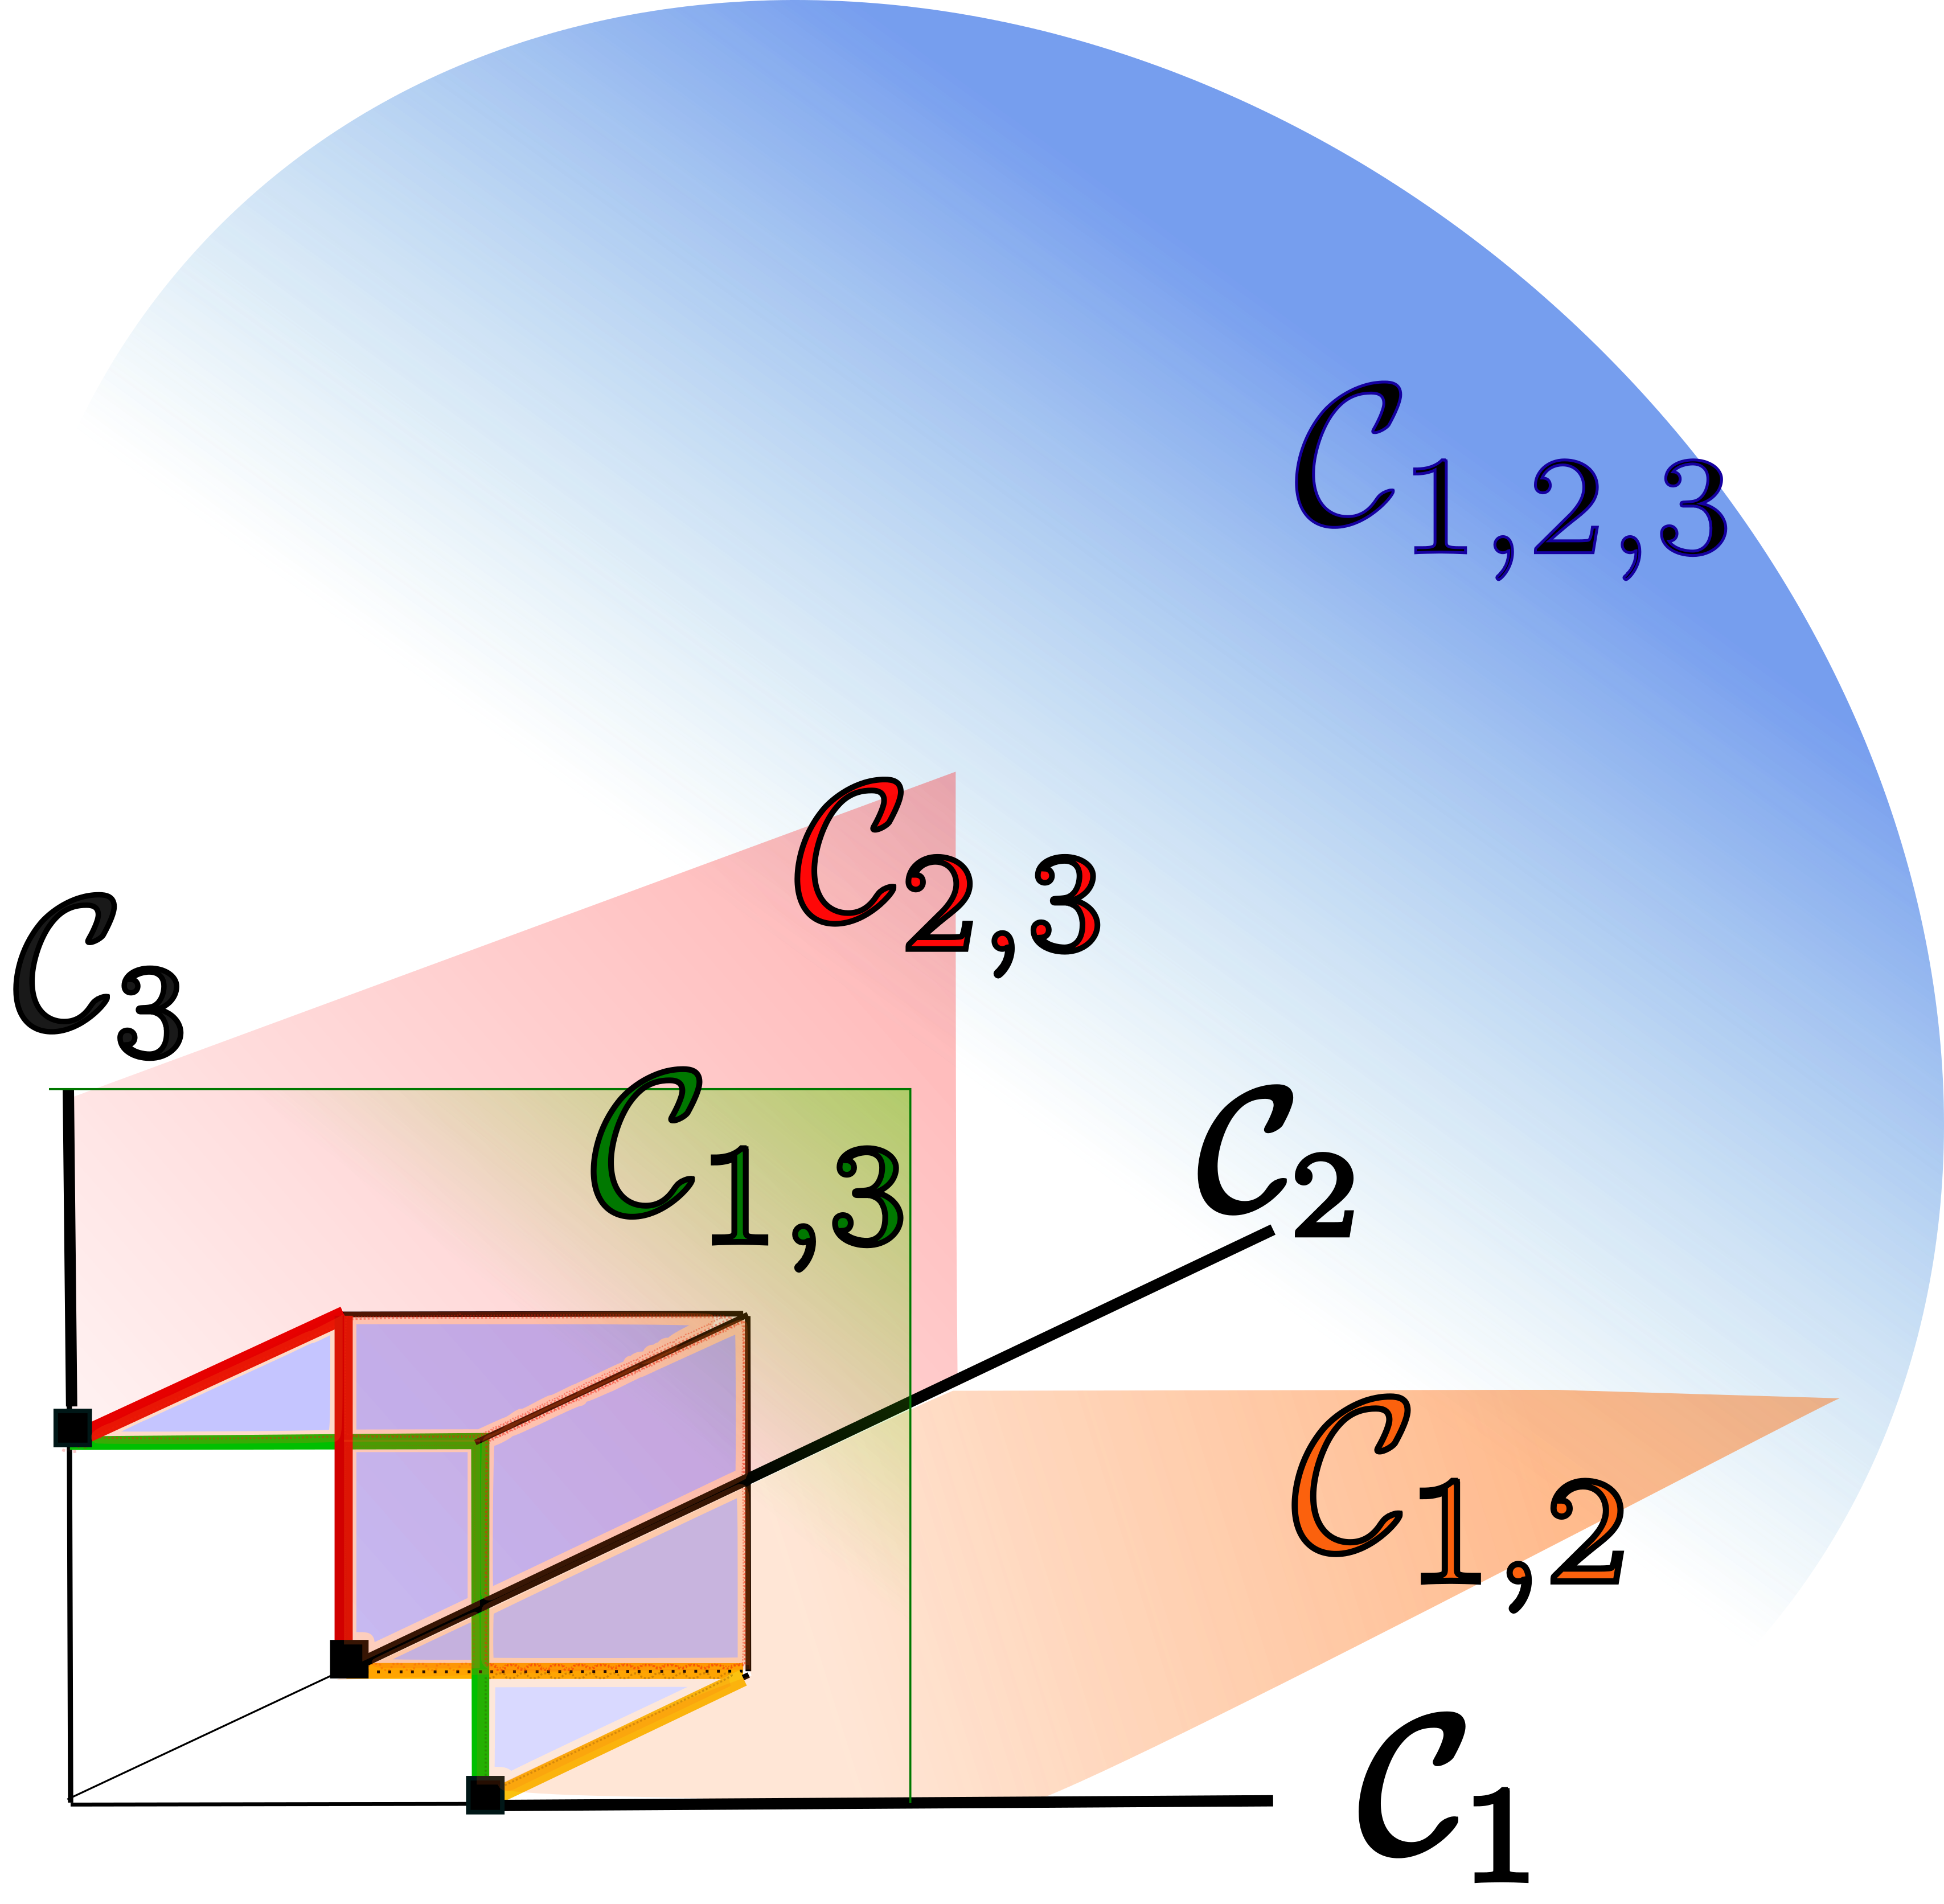
\includegraphics[scale=0.2]{fig_source/cone}
\captionof{figure}{Truncated cones in 3D}
\label{fig:3Dcones}
\end{minipage}\hfill
\begin{minipage}{0.5\linewidth}
\centering
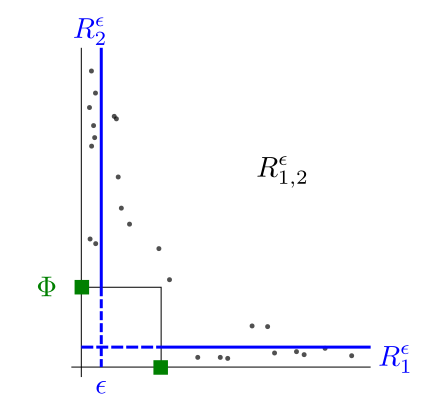
\includegraphics[width=0.64\linewidth]{fig_source/representation2D}
\captionof{figure}{Truncated $\epsilon$-cones in 2D}
\label{2Dcones}
\end{minipage}


This is done using $\epsilon$-thickened sub-cones $\cone_\alpha^\epsilon$, corresponding to $\epsilon$-thickened sub-spheres $\Omega_\alpha^\epsilon$, as shown in Figure~\ref{2Dcones} in the two-dimensional case.
We thus obtain an estimate $\widehat{\mathcal{M}}$ of the representation
$$\mathcal{M} = \{ \Phi(\Omega_{\alpha}):\; \emptyset \neq \alpha\subset\{1,\; \ldots,\; d \}\}.$$
Theoretically, recovering the $(2^{d}-1)$-dimensional unknown
vector $\mathcal{M}$ amounts to roughly approximating the support of $\Phi$ using the partition
$\{\Omega_\alpha, \alpha\subset\{1,\ldots,d\}, \alpha\neq \emptyset\}$, that is, determine which $\Omega_\alpha$'s have
nonzero mass (and evaluating the mass $\Phi(\Omega_\alpha)$), or equivalently, which $\Phi_\alpha$'s are nonzero. This support estimation is potentially
sparse (if a small number of $\Omega_\alpha$ have non-zero mass, \ie~Phenomenon~\textbf{1-}) and
potentially low-dimensional (if the dimensions of the sub-spheres $\Omega_\alpha$ with non-zero mass are low, \ie~Phenomenon~\textbf{2-}).

% Second, investigate how the angular measure $\Phi$ spreads its mass on the
% $\Omega_{\alpha}$'s, the theorical quantity $\Phi(\Omega_{\alpha})$ indicating to which extent extreme observations may occur in the `direction' $\alpha$ for $\emptyset \neq \alpha \subset \{1,\; \ldots,\; d \}$. 

% These two goals are achieved using empirical versions of
% the angular measure, evaluated on the $\epsilon$-thickened sub-spheres $\Omega_\alpha^\epsilon$.

\textbf{Anomaly Detection.}
Our proposed algorithm, DAMEX for Detecting Anomalies with Extremes, learns $\widehat{\mathcal{M}}$, a (possibly sparse and low-dimensional) representation of the angular measure, from which a scoring function can be defined in the context of anomaly detection.
The underlying assumption is that an observation is potentially abnormal if its `direction' (after a standardization of each marginal) is special regarding the other extreme observations. In other words, if it does not belong to the (sparse) representation $\widehat{\mathcal{M}}$. See Chapter~\ref{jmva} for details on how the scoring function is defined from this representation.
According to the benchmarks derived in this chapter, DAMEX significantly improves the performance (both in term of precision and of ROC curves) in extreme regions, inducing \eg~more vertical ROC curves near the origin.

\textbf{Theoretical grounds.}
From the work on the \stdf~estimation summarized in the previous sub-section~\ref{resume:stdf}, in particular from Theorem~\ref{thm-princ} and from the ideas used to prove Theorem~\ref{thm:l}, we are able to derive some theoretical guaranties for this approach.
%
Under non-restrictive assumptions standard in EVT (existence of the angular measure and continuous marginal c.d.f.), we obtain a non-asymptotic bound of the form
\begin{align*}
\sup_{\emptyset \neq \alpha \subset \{1,\; \ldots,\; d \}}~ |\widehat{\mathcal{M}}(\alpha)- \mathcal{M}(\alpha)|
~\le~  C d \left( \sqrt{ \frac{1}{\epsilon k}\log\frac{d}{\delta}} + M d\epsilon \right) + \text{bias}(\epsilon, k, n),
\end{align*}
with probability greater than $1-\delta$, where $k = k(n) \to \infty$ with $k(n) = o(n)$ can be interpreted as the number of data considered as extreme. 
The bias term goes to zero as $n \to \infty$, for any fixed $\epsilon$.


% \subsection{Algorithm and Application to Anomaly Detection}

% As explained above, the proposed algorithm, DAMEX for Detecting Anomalies with Extremes, learns a (possibly sparse and low-dimensional) representation of the angular measure. This representation is rough enough to control the variance in high dimension and accurate enough to gain information about the `probable directions' of extremes. From a theoretical perspective, it yields a --first-- non-parametric estimate of the angular measure in any dimension, restricted to a class of sub-spheres. %, with a non asymptotic bound on the error. 
% We believe that our method can also be used as a preprocessing stage, for dimensionality reduction purpose, before proceeding with a parametric or semi-parametric
% estimation of the angular measure which could benefit from the structural information issued in the first step.  Such applications are beyond the scope of this work and will be the subject of further research. 

% %The representation output by DAMEX may be exploited to detect anomalies among extremes.
% EVT has been intensively used in anomaly detection in the one-dimensional
% situation, see for instance \cite{Roberts99}, \cite{Roberts2000},
% \cite{Clifton2011}, \cite{Clifton2008}, \cite{Lee2008}.
% % Anomaly detection then relies on tail analysis of the variable of interest and naturally involves EVT.
% In the multivariate setup, however, there is --to the best of our
% knowledge--  no anomaly detection method
% relying on \textit{multivariate} EVT. Until now, the multidimensional case has only been  tackled by means of extreme value statistics
% based on univariate EVT. The major reason is 
% the difficulty to scale up existing multivariate EVT models
% with the dimensionality. In the present work we bridge the gap between the practice of anomaly detection and multivariate EVT by proposing a method which is
% able to learn a sparse `normal profile' of multivariate extremes and,
% as such, may be implemented to improve the accuracy of any usual anomaly detection algorithm.




% Let $\mb X_1,.\ldots,\mb X_n$ \iid random variables in $\mathbb{R}^d$ with joint
% (\emph{resp.} marginal) distribution $\mb F$ (\emph{resp.} $F_j$, $j =
% 1,\ldots,d$). Marginal standardization is a natural first step when
% studying the dependence structure in a multivariate setting. The
% choice of standard Pareto margins $V^j$ (with $\mathbb{P}(V^j > x ) =
% 1/x$, $x>0$) is convenient, and justified by multivariate extreme value theory (see Chapter~\ref{back:EVT}). One classical way to standardize is the
% probability integral transform, $T : X_i \mapsto V_i = ( (1- F_j
% (X_i^j))^{-1})_{1\leq j\leq d}$, $i = 1,\ldots,n$. 
% %
% Since the marginal distributions $F_j$ are unknown, we use their
% empirical counterpart $\hat F_j$, where $\hat F_j (x) =
% (1/n) \sum_{i=1}^n \mathds{1}_{X_i^j\le x}$. 
% Denote by $\hat T$ the rank transformation
% thus obtained and by $\hat V_i = \hat T(X_i)$ the corresponding rank-transformed
% observations. 

% Now, for a given subset of features $\alpha \subset \{1,...,d\}$
% the goal is to measure the
% % `correlation' within each
% %  at extreme levels, that is
% likelihood to observe a large $\mathbf{\hat V}$ such that $\hat V^j$ is `large' for all
% $j\in\alpha$, while the other $\hat V^j$'s ($j \notin \alpha$) are `small'.
% That is, estimating $\Phi(\Omega_\alpha)$.
% % Formally, one may %has to 
% % associate to each such $\alpha$ a coefficient
% % %$\mu_n^\alpha$ 
% % reflecting the degree of dependence between the
% % features $\alpha$ at extreme levels. %By definition of asymptotic dependence, 

% In relation to Section~\ref{context}, the appropriate way to
% give a meaning to `large' (\emph{resp.} `small') among extremes is in
% `radial' and `directional' terms, that is, $\| \mathbf{\hat V}\|>r$ (for some
% high radial threshold $r$), and $\hat V^j/\|\mathbf{\hat V}\| >\epsilon$
% (\emph{resp.} $ \le \epsilon$) for some small directional tolerance
% parameter 
% $\epsilon>0$.
% Introduce the truncated $\epsilon$-cones (see Fig.~\ref{2Dcones}):
% %\begin{align*}
% $ ~\mathcal{C}_\alpha^\epsilon~=~\big\{\mb v \ge 0,~\|\mb v\|_\infty \ge 1,~ v_i > \epsilon \|\mb v\|_\infty ~\text{ for } i
%  \in \alpha, ~~v_i \le \epsilon\|\mb v\|_\infty ~\text{ for } i \notin \alpha~ \big\},$
% %\end{align*}
% which defines a
% partition of $\mathbb{R}_+^{d}\setminus [0,1]^d$ for each fixed $\epsilon\ge 0$.
% This leads to  estimates %$\mu_n^{\alpha, \epsilon}$  of the form
% \begin{align}
% \label{mu_n}
% \Phi_n^{\alpha, \epsilon} = (n/k) \mathbb{\hat P}_n \left (  (n/k) \mathcal{C}_\alpha^\epsilon \right), 
% \end{align}
% \noindent
% where $\mathbb{\hat P}_n(.)=(1/n)\sum_{i=1}^n\delta_{\hat{\mb V}_i}(.)$ is the empirical probability distribution of the rank-transformed data and $k =
% k(n) \to \infty$ s.t. $k = o(n)$ as $n \to
% \infty$. %  Indeed we are to select the extreme observations to
% % study asymptotic dependence, from where the $\frac{n}{k}
% % \mathcal{C}_\alpha^\epsilon$ (
% The ratio $n/k$ plays the role of a large radial
% threshold $r$. 
% This estimator is justified by the result from multivariate EVT, $r \mathbb{P}(\mb V \in r A) \to \Phi(A)$ as $r \to \infty$ (see Chapter~\ref{back:EVT}).
% % From our standardization choice, counting points in
% % $(n/k)\,\mathcal{C}_{\alpha}^{\epsilon}$ boils down to
% % selecting, for each feature $j\le d$,   the `$k$ largest values' $X_i^j$
% % over the $n$ observations, whence the normalizing factor $\frac{n}{k}$.
% %Here and hereafter, $k =
% %k(n) >0$ is such that $k \to \infty$ and $k = o(n)$ as $n 
% %\infty$.
% %

% This heuristic yields the following algorithm~\ref{DAMEX-algo}.
% The complexity is in $O( dn\log n + dn) = O(dn\log n)$, where the first term on the left-hand-side comes from  computing the $\hat F_j(X_i^j)$ (Step 1) by sorting  the data
% (\emph{e.g.} merge sort). The second one comes from Step 2. 

% % \begin{center}
% % \fbox{
% % \begin{minipage}{0.95\linewidth}
% \begin{algorithm}[!tbh]
% \caption{DAMEX}
% \label{DAMEX-algo}
% {\bf Input:} parameters $\epsilon>0$,~~ $k = k(n)$,~~ $\Phi_{\min}\geq 0$.
% \begin{enumerate}
% \item Standardize \emph{via} marginal rank-transformation: $\hat V_i := \hat T(X_i) =  \big (1/(1- \hat F_j (X_i^j))\big)_{j=1,\ldots,d}$~. %\\where $\hat F_j (X_i^l) = \frac{1}{n}(rank(X_i^l)-1)$.
% % \item Let $k = n^{2/3}$, $\epsilon = \frac{1}{ k}$ 
% \item Assign to each $\hat V_i$ the cone $\mathcal{C}_\alpha^\epsilon$
%   it belongs to.  
% \item Compute  $\Phi_n^{\alpha, \epsilon}$ the estimate of the $\alpha$-mass of $\Phi$ from (\ref{mu_n}).\\
%  $\rightarrow$ yields: (small number of) cones with non-zero mass.
% \item (Optional) Set to $0$ the $\Phi_n^{\alpha,\epsilon}$ below some small
%   threshold $\Phi_{\min}\ge 0$ to eliminate cones with negligible mass
   
% \end{enumerate}
% {\bf Output:} (sparse) representation of the dependence
%   structure %$(\mu_n^{\alpha,\epsilon})_{\alpha\subset\{1,\ldots, d\}, \mu_n^{\alpha,\epsilon}>\mu_{\min}}$.
%  \begin{align*}
% \widehat{\mathcal{M}}(\alpha) := (\Phi_n^{\alpha,\epsilon})_{\alpha\subset\{1,\ldots, d\}, \Phi_n^{\alpha,\epsilon}>\Phi_{\min}}
%  \end{align*}

% \end{algorithm}
% % \end{minipage}
% % }
% % \end{center}

% This algorithm can directly be applied to anomaly detection.
% The underlying assumption is that an
% observation is potentially abnormal if its `direction' (after a standardization of each marginal) is special
% regarding the other extreme observations. In other words, if it
% does not belong to the (sparse) support of
% extremes.
% The degree of `abnormality' of a new observation $\mb x$ such that
% $\hat T(\mb x) \in \mathcal{C}_\alpha^\epsilon$ % an observation $X_i$
% should be related both to $\Phi_n^{\alpha, \epsilon}$ and the uniform
% norm $\|\hat T(\mb x)\|_\infty$ (angular and radial
% components). As a matter of fact, in the transformed space - namely the
% space of the $\hat V_i$'s - the asymptotic mass decreases as the
% inverse of the norm.
% Consider the  `\textit{directional tail region}' induced by $\mb x \in \mathcal{C}_\alpha^\epsilon$, 
% $A_{\mb x} =  \{\mb y  :
% T(\mb y) \in \mathcal{C}_\alpha^\epsilon\,,\;\|T(\mb y)\|_\infty \ge \|
% T(\mb x)\|_\infty\}.$
%  Then, if  $\|T(\mb x)\|_\infty$ is large enough, it can be shown that 
% $  \mathbb{P}( \mb X \in A_{\mb x} ) \simeq  \|\hat T(\mb x) \|_\infty^{-1} \Phi_n^{\alpha,\epsilon} $.
% We then set the scoring function $$s_n(\mb x):= (1/\|\hat T(\mb x)\|_\infty) \sum_{\alpha }\Phi_n^{\alpha, \epsilon} \mathds{1}_{\hat T(\mb x) \in \mathcal{C}_\alpha^\epsilon},$$
% which is thus an empirical version of
% $\mathbb{P}(\mb X\in A_{\mb x})$: the smaller $s_n(\mb x)$, the more abnormal the point $\mb x$ should be considered.


% \subsection{Theoretical grounds}

% From the work on the \stdf~estimation summarized in the previous Section~\ref{resume:stdf}, in particular from Theorem~\ref{thm-princ} and from the ideas used to prove Theorem~\ref{thm:l}, we are able to derive some theoretical guaranties for the approach described above. %  where non-asymptotic
% % bounds related to the statistical performance of a non-parametric
% % estimator of the \emph{stable tail dependence function} (STDF), another 
% % functional measure of the dependence structure of extremes,  are
% % established.  
% % However, even in the case of a sparse angular measure, the support of
% % the STDF would not be so, since the latter functional is  an
% % integrated version of the former. Also, 
% % in many applications, it is more convenient to work with % an alternative (distributional)
% %  the {angular measure}. Indeed, it provides direct information about the probable `directions' of extremes. % , that is, the relative contribution
% % % of each components of the `largest' observations  (where `large' may be 
% % % understood \emph{e.g.} in the sense of the infinity norm on the input
% % % space). We emphasize again that estimating these `probable relative contributions' is a major concern in many fields
% % % involving  the management of risks from multiple sources, \emph{e.g.}\,portfolio monitoring, insurance,
% % % environmental risk management and anomaly detection. 
% % To the best of our knowledge, non-parametric estimation of the angular
% % measure has only been treated in the two dimensional case, in
% % \cite{Einmahl2001} and \cite{Einmahl2009}, in an asymptotic
% % framework.

% Under non-restrictive assumptions standard in EVT (existence of the angular measure and continuous marginal c.d.f.), we obtain a non-asymptotic bound of the form
% \begin{align*}
% \sup_{\emptyset \neq \alpha \subset \{1,\; \ldots,\; d \}}~ |\widehat{\mathcal{M}}(\alpha)- \mathcal{M}(\alpha)|
% ~\le~  C d \left( \sqrt{ \frac{1}{\epsilon k}\log\frac{d}{\delta}} + M d\epsilon \right) + \text{bias}(\epsilon, k, n),
% \end{align*}
% with probability greater than $1-\delta$, where $k = k(n) \to \infty$ with $k(n) = o(n)$ can be interpreted as the number of data considered as extreme. 
% The bias term goes to zero as $n \to \infty$, for any fixed $\epsilon$.




% \subsection{Empirical guaranties}
%  The main purpose of Algorithm~\ref{DAMEX-algo} is to deal with extreme data. We evaluate its performance on such region and compare it with a standard anomaly detection algorithm, the Isolation Forest (iForest) algorithm, see Section~\ref{sec:impl} below, which we chose in view of its established high performances (\cite{Liu2008}) and its ability to handle large dimensional data. 
% The two algorithms are trained and tested on the same datasets, the test set being restricted to some extreme region.
% Five reference real-word datasets in anomaly detection are considered. The experiments are performed in a novelty detection framework (the training set consists of normal data). In a  non-supervised framework (training set including abnormal data), the improvements brought by the use of DAMEX are less significant, but the precision score is still increased when the recall is high (high rate of true positives), inducing more vertical ROC curves near the origin.
% DAMEX significantly improves the performance (both in term of precision and of ROC curves) in extreme regions for each dataset.

% % XXX: comparaison avec LOF, OCSVM and EllipticEnvelop when possible?\\
% % XXX: study combination DAMEX with other classical AD?



\section{Heuristic approaches}
\label{resume:sec:heuristic}

The two contributions in this section are of heuristic nature and not yet supported by statistically sound theoretical results. Although this ongoing work has not been published yet and will certainly be completed in the near future, we believe that it has its place in our manuscript, given the numerous convincing numerical experiments we carried out and the rationale behind the approaches promoted we gave.
%
These two contributions address two major challenges in anomaly detection:

\begin{itemize}
\item How to evaluate unsupervised anomaly detection in practice?
\item How to grow random forests with only one class available?
\end{itemize}

The first point has been partially addressed in Section~\ref{resume:scoring} with MV and EM curves.
However, these two criteria have originally been introduced to build scoring functions \emph{via} Empirical Risk Minimization (ERM), and no study has been made on their use to evaluate scoring functions as ROC or PR criteria do.
Besides, their use to measure the quality of a scoring function $s_n$ involves the computation of the Lebesgue measure  $\leb(s_n \ge u)$, which is very challenging in high dimensional frameworks. 

The two proposed approaches are heuristic-based, and no theoretical guarantees such as consistency or convergence rates are derived. However, extensive benchmarks show the relevance of these approaches.

\subsection{Evaluation of anomaly detection algorithms}
\label{resume:evaluation}
This is a summary of Chapter~\ref{chap:evaluation}, which is based on a workshop paper \citep{ICMLworkshop16} and a work to be submitted \citep{NIPS16evaluation}.


When sufficient labeled data are available, classical criteria based on ROC \citep{Provost1997, Provost1998, Fawcett2006} or PR \citep{Davis2006, Clemencon2009} curves can be used to compare the performance of unsupervised anomaly detection algorithms. However, in many situations, few or no data are labeled. This calls for alternative criteria one can compute on non-labeled data.

While excess-mass and mass-volume curves quantities have originally been introduced to build scoring functions \emph{via}
Empirical Risk Minimization (ERM), the MV-curve has been used recently for the calibration of the One-Class SVM \citep{Thomas2015}.
When used to attest the quality of some scoring function, the volumes induced become unknown and must be estimated, which is challenging in large dimension if no prior knowledge on the form of these level sets is available.
%
Besides, the accuracy of EM or MV curves as evaluation criteria has not been studied yet.
%
Summarized in this section and as a contribution of this thesis, numerical performance scores based on EM and MV criteria (that do not require labels) are empirically shown to discriminate accurately (\wrt~ROC or PR based criteria) between algorithms.
%These criteria are based on existing Excess-Mass (EM) and Mass-Volume (MV) curves, which generally cannot be well estimated in large dimension.
A methodology based on feature sub-sampling and aggregating is also described and tested. This extends the use of these criteria to high-dimensional datasets and solves major drawbacks inherent to standard EM and MV curves.

Recall that the MV and EM curves of a scoring function $s$ can be written as
\noindent
\begin{align}
\label{intro:MV-def}
 MV_s(\alpha) &= \inf_{u \ge 0}~~ \leb(s \ge u) ~~\st~~\mathbb{P}(s(\mb X) \ge u) \ge \alpha\\
\label{intro:EM-def}
 EM_s(t) &= \sup_{u \ge 0}~~ \mathbb{P}(s(\mb X) \ge u) ~-~ t \leb(s \ge u)
\end{align}
for any $\alpha\in (0,1)$ and $t >0$.
%
The optimal curves are $MV^* = MV_f = MV_{T \circ f}$ and $EM^* = EM_f = EM_{T \circ f}$ for any increasing transform $T: \text{Im(f)} \to \mathbb{R}$.
%
As curves cannot be trivially compared, consider the $L^1$-norm $\|.\|_{L^1(I)}$ with $I\subset \rset$ an interval. As $MV^*=MV_f$ is below $MV_s$ pointwise, $\argmin_s \| MV_s - MV^* \|_{L^1(I)} = \argmin \| MV_s \|_{L^1(I)} $. We thus define
$\crit^{MV}(s) = \| MV_s \|_{L^1(I^{MV})},$ which is equivalent to consider $\| MV_s - MV^* \|_{L^1(I^{MV})}$ as mentioned in the introduction. As we are interested in evaluating accuracy on large density level-sets, one natural interval $I^{MV}$ would be for instance $[0.9, 1]$. However, MV diverges in $1$ when the support is infinite, so that we arbitrarily take $I^{MV} = [0.9, 0.999].$
The smaller is $\crit^{MV}(s)$, the better is the scoring function $s$.
%
Similarly, we consider $\crit^{EM}(s) = \| EM_s \|_{L^1(I^{EM})}, $ this time with $I^{EM} = [0,EM^{-1}(0.9)],$ where $EM_s^{-1}(0.9) := \inf\{t\ge 0,~ EM_s(t) \le 0.9\}$, as $EM_s(0)$ is finite (equal to $1$). % We point out that such small values of $t$ correspond to large level-sets. Also in practice, we have observed that
% $EM_s^{-1}(0.9)$ (as well as $EM_f^{-1}(0.9)$) varies significantly depending on the dataset. Generally, for datasets in large dimension, it can be % $\widehat{EM}_s^{-1}(0.9)$ is
% very small (in the experiments, smallest values are of order $10^{-7}$) as it is of the same order of magnitude as the inverse of the total support volume.

As the distribution $F$ of the normal data is generally unknown, MV and EM curves must be estimated. Let $s\in \mathcal{S}$ and $\mb X_1,\; \ldots,\; \mb X_n$ be an i.i.d. sample with common distribution $F$ and set $\mathbb{P}_n(s \ge t)=\frac{1}{n}\sum_{i=1}^n\mathds{1}_{s(\mb X_i)\geq t}.$ The empirical MV and EM curves of $s$ are then simply defined as empirical version of \eqref{intro:MV-def} and \eqref{intro:EM-def}, 
\begin{align}
\label{MV-def-emp}
\widehat{MV}_s(\alpha) = \inf_{u \ge 0} \left\{ \leb(s \ge u) ~~\st~ \mathbb{P}_n(s \ge u) \ge \alpha \right\}
\end{align}
\begin{align}
\label{EM-def-emp}
\widehat{EM}_s(t) = \sup_{u \ge 0} \mathbb{P}_n(s \ge u) ~-~ t \leb(s \ge u)
%\lambda_s \circ \alpha_s^{-1}(\alpha),
\end{align}
%
%
Finally, we obtain the empirical EM and MV based performance criteria:
\begin{align}
\label{eq:standard_emp_EM}\widehat{\crit}^{EM}(s) &= \| \widehat{EM}_s \|_{L^1(I^{EM})}  &&I^{EM} = [0,\widehat{EM}^{-1}(0.9)],\\
\label{eq:standard_emp_MV}\widehat{\crit}^{MV}(s) &= \| \widehat{MV}_s \|_{L^1(I^{MV})}  &&I^{MV} = [0.9, 0.999].
\end{align}
%
% As the distribution $F$ is generally unknown, excess-mass curves must be estimated. Let $s\in \S$ and $\mb X_1,\; \ldots,\; \mb X_n$ be an i.i.d. sample with common distribution $F$ and set $$\widehat{\alpha}_s(t)=(1/n)\sum_{i=1}^n\mathds{1}_{s(X_i)\geq t}.$$ The empirical $EM$ curve of $s$ is then defined as $$\widehat{EM}_s(t)=\sup_{u>0}\{ \widehat{\alpha}_s(u)-t\lambda_s(u)\}.$$ In practice, just as with the mass-volume criterion (drawback \textbf{1}), it may be difficult to estimate the volume $\lambda_s(u)$ and Monte-Carlo approximation can naturally be used for this purpose.

% Note that in practice, the volume $\leb(s \ge u)$ is estimated using Monte-Carlo approximation, which only applies to small dimensions.
% %
% This is a major drawback for the use of excess-mass or mass-volume criteria in high dimensional framework, if no prior knowledge on the form of these level sets is available. Besides, there has been no work yet dealing with EM or MV curves as evaluation criteria, as they have originally been introduced to build scoring scoring function via ERM.
%
The methodology to scale the use of the EM and MV criteria to large dimensional data consists in sub-sampling training \emph{and} testing data along features, thanks to a parameter $d'$ controlling the number of features randomly chosen for computing the (EM or MV) score. Replacement is done after each draw of features $F_1,\ldots,F_{m}$. A partial score $\widehat \crit_k^{MV}$ (resp. $\widehat \crit_k^{EM}$) is computed for each draw $F_k$ using \eqref{eq:standard_emp_EM} (resp. \eqref{eq:standard_emp_MV}). The final performance criteria are obtained by averaging these partial criteria along the different draws of features. This methodology is described in Algorithm~\ref{algo:EMMV}.
%
\begin{algorithm}[!tbh]
\caption{~~High-dimensional EM/MV: evaluate AD algorithms on high-dimensional data}
\label{algo:EMMV}
\begin{algorithmic}
  \STATE \textbf{Inputs}: AD algorithm $\mathcal{A}$, data set $X = (x^j_i)_{1 \le i \le n, 1 \le j \le d }$, feature sub-sampling size $d'$, number of draws $m$.
  \FOR{$k=1,\ldots,m$}
    \STATE{randomly select a sub-group $F_k$ of $d'$ features}
    \STATE{compute the associated scoring function $\widehat s_{k} = \mathcal{A}\big((x^j_i)_{1 \le i \le n,~j \in F_k}\big)$}
    \STATE compute $\widehat{\crit}_k^{EM} = \| \widehat{EM}_{\widehat s_k} \|_{L^1(I^{EM})}$ using \eqref{eq:standard_emp_EM} or $\widehat{\crit}_k^{MV} = \| \widehat{MV}_{\widehat s_k} \|_{L^1(I^{MV})}$ using \eqref{eq:standard_emp_MV}
  \ENDFOR 
  \STATE \textbf{Return} performance criteria: $$\widehat{\crit}^{EM}_{high\_dim} (\mathcal{A})= \frac{1}{m} \sum_{k=1}^m\widehat \crit_k^{EM} \text{~~~~(idem for MV)}$$
\end{algorithmic}
\end{algorithm}

Low-dimensional and high-dimensional EM/MV are tested \wrt~three classical AD algorithms. A wide range on real labeled datasets are used in the benchmark.
Experiments show that when one algorithm has % \emph{clearly} (according to both EM and PR scores)
better performance than another on some fixed dataset, according to both ROC and PR AUCs, one can expect to recover it without using labels with an accuracy of $82\%$ in the novelty detection framework, and $77\%$ in the unsupervised framework.


\subsection{One-Class Random Forests}
\label{resume:ocrf}
This is a summary of Chapter~\ref{chap:ocrf}, which is based on work \citep{OCRF16} to be submitted.

%Scoring functions built by optimizing EM or MV criteria usually not perform well. 

Building accurate scoring functions by optimizing EM or MV criteria is very challenging in practice, just as building classifiers by optimizing the ROC curve (\cite{Clemencon2010}) in the supervised framework.
%
More work is needed for these methods to be efficient in practice, particularly for the choice of the class of sets on which the optimization is done.
%
Indeed, % optimization is done over some class of scoring functions
this class is \emph{hopefully rich enough to provide a good approximation while simple enough to control the convergence rate}. This compromise is hard to achieve, especially in high dimension when no prior knowledge on the shape of the level sets is available. 
%
% In addition, if criterion optimization is useful when no intuition is available on the underlying problem, this is not the case in anomaly detection. We usually do not try to minimize ROC curves to have a good classifier, and a doctor usually does not health people by trying to optimize tensiometer or stethoscope measurements. 
%
% To derive guaranties of theoretical nature (namely to attest the relevance of the algorithm in terms of \eg~ROC or EM/MV criteria), optimizing these evaluation criteria is often an efficient way. 
% But this does not remains true in terms of empirical performance. 
In this section, we propose a heuristic approach to build scoring functions using Random Forests (RFs) \citep{Breiman2001, Genuer2008, Biau2008, Biau2016}. % , which are an intuitive way of performing classification and regression.
More formally, we adapt RFs to the one-class classification framework by introducing one-class splitting criteria.

Standard RFs are estimators that fit a number of decision tree
classifiers on different random sub-samples of the dataset.
Each tree is built recursively, according to a splitting criterion based on
some impurity measure of a node. The prediction is done by an average over each tree prediction. In classification the averaging is based on a majority vote.
Few attempts to transfer the idea of RFs to one-class
classification have already been made \citep{Desir12, Liu2008, Shi2012}.
%, Clemencon2014}. On ne cite pas clemencon2014 car leur algorythm treeRank n'est pas des RFs (base estimator = non-symetric ranking trees) (en fait unsupervisedTreeRank c'est juste une modif triviale de TreeRank en considerant des volumes)
%
No algorithm structurally extends (without second class sampling and without alternative base estimators) RFs to one-class classification.

We introduce precisely such a methodology. It builds on a natural adaptation of two-class % Gini improvement proxy, yielding a one-class Gini-based criterion specially designed for
splitting criteria to the one-class setting, as well as an adaptation of the two-class majority vote.
In addition, it turns out that the one-class model promoted here corresponds to the asymptotic behavior of an adaptive (with respect to the tree growing process) outliers generating methodology.

\textbf{One-class Model with parameters ($n$, $\boldsymbol{\alpha}$).}
We consider a random variable $ X:\Omega \to \mathbb{R}^d$ \wrt~a probability space $(\Omega, \mathcal{F}, \mathbb{P})$.
The law of $X$ depends on another \rv~$y \in \{0,1\}$, verifying $\mathbb{P}(y=1)=1-\mathbb{P}(y=0)=\alpha$. We assume that conditionally on $y=0$, $ X$ follows a law $F$, and conditionally on $y=1$ a law $G$:
\begin{align*}
 X ~|~ y=0 ~~\sim~~ F, &~~~~~~~~~~  \mathbb{P}(y=0)=1-\alpha, \\
 X ~|~ y=1 ~~\sim~~ G, &~~~~~~~~~~  \mathbb{P}(y=1)=\alpha.
\end{align*}
%
We model the one-class framework as follows. Among the $n$ \iid~observations, we only observe those with $y=0$ (the normal behavior), namely $N$ realizations of $( X ~|~ y=0)$, where $N$ is itself a realization of a \rv~$\mb N$ of law $\mb N \sim \text{Bin}\big(n, (1-\alpha)\big)$, the binomial distribution with parameters $(n, p)$. As outliers are not observed, we classically assume that $G$ follows a uniform distribution on the hyper-rectangle $\mathcal{X}$ containing all the observations, so that $G$ has a constant density $g(x) \equiv 1 / \leb(\mathcal{X})$ on $\mathcal{X}$. This assumption \emph{will be removed} in the adaptive approach, where no prior distribution is assumed for the outliers.
%laisser une ligne car fin du model one class

One-class empirical analogues of two-class impurity measures are then obtained by replacing the quantities relative to the normal behavior by their empirical versions.
The quantities relative to the unobserved second class (abnormal behavior) are naturally expressed using the uniform distribution assumption.

In this way, our one-class impurity improvement function corresponds to the two-class one, where empirical second class quantities have been replaced by their expectation assuming a uniform distribution.

But it also induces a major problem: those expectations, which are proportional to the volume of the node at stake, become very small when going deeper in the tree. In the two-class framework, the corresponding problem is when the second class is highly under-represented in the neighborhood of the observations. 
%
As we assume the second class to be uniform on a hyper-rectangle containing all the observations, this fact was expected, especially in large dimension (curse of dimensionality). 
%
As the quantities relative to the second class are very close to zero, one observes that the impurity criterion becomes constant when the split varies, and then useless.

\textbf{Adaptive approach.}
%
A solution is to chose adaptively (\wrt~the volume of each node) the number $\alpha n$, which can be interpreted as the number of (hidden) outliers. Recall that neither $n$ nor $\alpha$ is observed in One-Class-Model($n$, $\alpha$) defined above. 

The idea is to make $\alpha(t) \to 1$, $n(t) \to \infty$ when the volume of node $t$ goes to zero.
%
In other words, instead of considering one fixed general model One-Class-Model($n$, $\alpha$), we adapt it to each node $t$, considering One-Class-Model($n(t)$, $\alpha(t)$) \emph{before searching the best split}. We still consider the $N$ normal observations as a realization of this model. When growing the tree, using One-Class-Model($n(t)$, $\alpha(t)$) allows to maintain a non-negligible expected proportion of outliers in the node to be split, even when its volume becomes close to zero.
Of course, constraints have to be made to ensure consistency between all these models.
%
For instance, recalling that the number $N$ of normal observations is a realization of $\mb N$ following a Binomial distribution with parameters $(n, 1-\alpha)$, a first natural constraint on $\big(n(t), \alpha(t)\big)$ is
\begin{align}
\label{constraint1}
(1-\alpha)n = \big(1-\alpha(t)\big) \cdot n(t) \text{~~~~~for all~~} t,
\end{align}
so that the expectation of $\mb N$ remains unchanged. 
Then the asymptotic model (when the volume of $t$ goes to $0$) consists in fact in assuming that the number $N$ of normal data we observed is a realization of a Poisson distribution $\mathcal{P}\big((1-\alpha)n\big)$, and that an infinite number of outliers have been hidden. In the two class framework, this corresponds to observing an infinite number of outliers distributed closely around, outside and inside the support of the normal distribution, breaking the curse of dimensionality when using uniformly distributed outliers (see Chapter~\ref{chap:ocrf} for details).

\begin{remark}[\textbf{Basic idea behind the adaptive approach}]
This work corresponds in fact to the following simple idea that allows us to split a node without examples of the second class.
Each time we are looking for the best split for a node $t$, we simply replace (in the 2-class impurity decrease to be maximized) the second class proportion in the left node $t_L$ by the proportion expectation $volume(t_L)/volume(t)$ (idem for the right node).
It ensures that one child node tries to capture the maximum number of observations with a minimal volume, while the other child looks for the opposite. %Such volume constraint/mass objective are similarly used to define minimum-volume sets.
\end{remark}


\begin{remark}[\textbf{No sampling}]
The corresponding sampling method is the following: for each note $t$ to be splitted containing $n_t$ observations (inliers), generate $n_t$ uniform outliers over the corresponding cell to optimize a two-class splitting criterion. We precisely \emph{avoid sampling} the outliers by using the proportion expectation $volume(t_L)/volume(t)$.
\end{remark}



\textbf{One-Class RF algorithm.} Let us summarize the algorithm in its most generic version.
It has $7$ parameters:
$max\_samples$, $max\_features\_tree$, $max\_features\_node$, $\gamma$, $max\_depth$, $n\_trees$, $s_k$.
%
Each tree is classically grown on a random subset of both the input samples and the input features \citep{Ho1998, Panov2007}.
This random subset is a sub-sample of size $max\_samples$, with $max\_features\_tree$ variables chosen at random without replacement (replacement is only done after the tree is grown). The tree is built by minimizing 
a one-class version of the Gini criterion \citep{Gini1912}, obtained by replacing empirical quantities related to the (unobserved) second class by population ones. These correspond to a weighted uniform distribution, the weight increasing when the volume of the node decreases, in order to avoid highly unbalanced classes (volume vs. observations). Indeed when their depth increases, the nodes tend to have smaller volumes while keeping as much (normal) observations as they can.

New nodes are built (by minimizing this criterion) until the maximal depth $max\_depth$ is achieved.
% define a large number of geometric features and search over a random selection
% of these for the best split at each node
% In addition, this is done
Minimization is done as introduced in \citep{Amit1997}, by defining a large number $max\_features\_node$ of geometric features and searching over a random selection of these for the best split at each node.
%
The forest is composed of a number $n\_trees$ of trees. The predicted score of a point $x$ is given by $s_k(x)$, which is either the stepwise density estimate (induced by the forest) around $x$, the local density of a typical cell containing $x$ or the averaged depth of $x$ among the forest. Chapter~\ref{chap:ocrf} formally defines the one-class splitting criteria and provides an extensive benchmark of state-of-the-art anomaly detection algorithms.








\section{Scikit-learn contributions}
\label{sec:impl}

As an other contribution of this thesis, two classical anomaly detection algorithms, Isolation Forest and Local Outlier Factor have been implemented and merged on scikit-learn. These algorithms are presented in the Background Part, Section~\ref{sec:AD_sklearn}. % on Anomaly Detection in Scikit-Learn. 

Scikit-learn, see \cite{sklearn2011}, is an open-source library providing well-established machine learning methods.
It is a Python module, the latter language being very popular for scientific computing, thanks to its high-level interactive nature. % Python is enjoying this recent years a strong expansion both in academic and industrial settings. Scikit-learn takes advantage of this favourable backdrop and extends this general-purpose programming language with machine learning operation: 
Scikit-learn provides a composition mechanism (through a \emph{Pipeline} object) to combine estimators, preprocessing tools and model selection methods in such a way the user can easily construct complex ad-hoc algorithms.
%
The development is done on \emph{Github}\footnote{https://github.com/scikit-learn}, a Git repository hosting service which facilitates collaboration, as coding is done in strong interaction with other developers. Because of the large number of developers, emphasis is put on keeping the project maintainable, \eg~by avoiding duplicating code at the price of a reasonable loss of computational performance.%up to pay (reasonably) in computational performance. 


This contribution was supervised by Alexandre Gramfort and was funded by the Paris Saclay Center for Data Science. It also includes work for the scikit-learn maintenance like resolving issues and reviewing other contributors' pull requests.

% XXX: add contribution with A.Muller


\section{Conclusion and Scientific Output}
\label{intro:concl}
The contributions of this thesis can be summarized as follows. 

First, an adequate performance criterion called Excess-Mass curve is proposed (Section~\ref{resume:em-curve}), in order to compare possible candidate scoring function and to pick one eventually. 
The corresponding publication is \cite{AISTAT15}:
\begin{itemize}
\item On Anomaly Ranking and Excess-Mass Curves. (AISTATS 2015).\\
Authors: Goix, Sabourin, and Clémençon. 
\end{itemize}

% This is a major drawback for its use in high dimensional framework, if no prior knowledge on the form of these level sets is available. 


%However, to measure with this criterion the quality of a scoring function $s_n$, volume of level sets of $s_n$ have to be compute which is a considerable drawback for its use in high dimensional framework, if no prior knowledge on the form of these level sets is available.

As a second contribution, we bring advances in multivariate EVT by providing non-asymptotic bounds for the estimation of the STDF, a functional characterizing the extreme dependence structure (Section~\ref{resume:stdf}). The corresponding publication is \cite{COLT15}:
\begin{itemize}
\item Learning the dependence structure of rare events: a non-asymptotic study. (COLT 2015).\\
Authors: Goix, Sabourin, and Clémençon.
\end{itemize}

The third contribution is to design a statistical method that produces a (possibly sparse) representation of the dependence structure of extremes, while deriving non-asymptotic bounds to assess the accuracy of the estimation procedure (Section~\ref{resume:sec:JMVA}).
%
This contribution also includes a multivariate EVT-based algorithm which returns a scoring functions defined in extreme regions. This directly applies to anomaly detection as an abnormality score.
The corresponding publications are \cite{AISTAT16}, \cite{NIPSWORKSHOP15} and \cite{ARXIV16}:
%
\begin{itemize}
\item Sparse Representation of Multivariate Extremes with Applications to Anomaly Ranking. (AISTATS 2016 and NIPS 2015 Workshop on Nonparametric Methods for Large Scale Representation Learning).\\
Authors: Goix, Sabourin, and Clémençon.
\item Sparse Representation of Multivariate Extremes with Applications to Anomaly Detection. (Under review for Journal of Multivariate Analysis).\\
Authors: Goix, Sabourin, and Clémençon.
\end{itemize}





As a fourth contribution, we show (empirically) that EM or MV based criteria are able to discriminate accurately (\wrt~ROC or PR based criteria) between scoring functions in low dimension. Besides, we propose a methodology based on feature sub-sampling and aggregating to scale the use of EM or MV to higher dimensions.
The corresponding publications are \cite{ICMLworkshop16} and \cite{NIPS16evaluation}:
\begin{itemize}
\item How to Evaluate the Quality of Unsupervised Anomaly Detection Algorithms? (ICML 2016, Workshop on Anomaly Detection). % Co-winner of the Best Paper Award, sponsored by Google.
  \\
Author: Goix. 
\item How to Evaluate the Quality of Unsupervised Anomaly Detection Algorithms? (to be submitted).\\ Authors: Goix and Thomas. 
\end{itemize}


The fifth contribution of this thesis is to develop an efficient heuristic for building accurate scoring functions. This is done by generalizing random forests to one-class classification. The corresponding work (to be submitted) is \cite{OCRF16}: 
\begin{itemize}
\item One-Class Splitting Criteria for Random Forests with Application to Anomaly Detection. (to be submitted).\\
Authors: Goix, Brault, Drougard and Chiapino.
\end{itemize}



As a last contribution, two classical anomaly detection algorithms have been implemented and merged on scikit-learn. They are used in this dissertation for empirical comparison purpose to attest the relevance of the forementionned approaches.
The pull requests of these two contributions are available here:
\begin{itemize}
\item https://github.com/scikit-learn/scikit-learn/pull/4163  (Isolation Forest)
\item https://github.com/scikit-learn/scikit-learn/pull/5279 (LOF)
\end{itemize}


% Eventually, we would like to notice that there still seems to be a significant gap to fill between theory and practice in anomaly detection. Trying to derive an algorithm supported by a theoretical analysis often affects the algorithm construction in such a way that it limits its efficiency in practice.
% On the opposite side, when trying to develop an algorithm which performs well in practice before thinking about any theoretical guaranties, it is often difficult to derive a statistical analysis. In this thesis, contributions have been made on both of these sides. Besides, the contribution on the sparse representation of multivariate extreme belongs to both theoretical and practical sides: it can be viewed as an efficient heuristic supported by a mathematical analysis from the extreme value theory, as well as an algorithm designed by this theory which can compete with state-of-the-art anomaly detection algorithms.


\paragraph{Context of this work.}
This thesis was carried out in the STA (Statistiques et Applications) team of the Signal and Image Processing (TSI) department at Telecom ParisTech. The contributions presented in this thesis were supported by Ecole Normale Supérieure de Cachan via a `contrat doctoral pour normalien' and by the industrial chair `Machine Learning for Big Data' from Telecom ParisTech. The scikit-learn contributions have been supported by the Paris Saclay Center for Data Science regarding the collaboration with Alexandre Gramfort, and by the forementioned machine learning chair as regards the collaboration at New York University with Andreas Müller.

\paragraph{Outline of the thesis.}
This dissertation is organized as follows. 
\begin{itemize}
\item Part~\ref{part:background} gathers the background work relevant to this thesis:

Chapter~\ref{chap:back_concentration} presents general results on measure concentration inequalities; 

Chapter~\ref{back:EVT} provides a concise background on extreme value theory;

Chapter~\ref{back:AD_scikit} reviews classical anomaly detection algorithms used in the benchmarks and provides illustrative examples with the scikit-learn library. It also presents relating code contributions.

\item Part~\ref{part:struct} deals with theoretical performance criteria for the anomaly ranking task:

Chapter~\ref{aistat:chap} presents the details on anomaly ranking and excess-mass curve, as summarized above Section~\ref{resume:scoring}; %The corresponding published work is \cite{AISTAT15}.

\item Part~\ref{part:vect} focuses on EVT-based methods for anomaly detection:

Chapter~\ref{colt} deals with the stable tail dependence function as summarized above in Section~\ref{resume:stdf}; %The corresponding publication is \cite{COLT15};

Chapter~\ref{jmva} describes how scoring functions can be build using EVT, as previously summarized in Section~\ref{resume:sec:JMVA}.
%The corresponding publications are \cite{NIPSWORKSHOP15}, \cite{AISTAT16} and submitted work \cite{ARXIV16}.


\item Part~\ref{part:heuristic} gathers two efficient heuristic-based methodologies:

Chapter~\ref{chap:evaluation} deals with the evaluation of anomaly detection algorithms, as summarized above Section~\ref{resume:evaluation}; %Chapter~\ref{resume:evaluation}.
%The corresponding publications are \cite{ICMLworkshop16} and \cite{NIPS16evaluation}.

Chapter~\ref{chap:ocrf} presents the details % on one class splitting criteria 
  (summarized above Section~\ref{resume:ocrf}) on one-class random forests.
%The corresponding submitted work is \citep{OCRF16};


\end{itemize}

%%\numberwithin{section}{chapter}

\part{Preliminaries}\label{part:background}

\chapter{Concentration Inequalities from the Method of bounded differences}
\label{chap:back_concentration}
% XXXX TODO: add memoire + CONCENTRATION
\begin{chapabstract}
This chapter presents general results on measure concentration inequalities, obtained via martingale methods or with Vapnik-Chervonenkis theory. In the last section~\ref{sec:concentration-contrib} of this chapter, a link is also made with contributions presented in Chapter~\ref{colt} which builds on some concentration inequality stated and proved here.
\end{chapabstract}

Note: 
In addition to a review of popular results and sketches of proofs from the existing literature, the last section~\ref{sec:concentration-contrib} of this chapter presents an original contribution;
% The only contribution here lies in the last section~\ref{sec:concentration-contrib} of this chapter, where a
a VC-type inequality is proved using a Bernstein-type concentration inequality. A corollary of this VC-type inequality focusing on maximal deviation on low-probability regions is needed in Chapter~\ref{colt}.

We recommend \cite{McDiarmid98} and \cite{Janson2002} for good references on this subject, and \cite{Massart2007, BLM2013} for a extensive review on concentration inequalities.
%
About the impact of the concentration of measure phenomenon in EVT, see \cite{Boucheron2012, Boucheron2015} and the PhD thesis \cite{ThomasMaud2015}.
%
References on classification and statistical learning theory (not gathered by this background part), include \cite{Vapnik74, Devroye96, Bousquet04, BBL05, Bishop2006, Friedman2001, Vapnik2013} 


%  Ce document présente des résultats généraux sur les inégalités de concentration de mesure et quelques applications, notamment aux graphes aléatoires.
% Il est basé sur les articles de Colin McDiarmid "Concentration", de Terence Tao "Talagrand's concentration inequality", et de Svante Janson "On concentration of probability".
% Dans ce travail, j'ai choisi de mettre en relation les trois articles de la facon suivante : J'utilise l'article de McDiarmid pour illustrer et démontrer dans un cadre plus général les résultats fondamentaux exposés dans l'article de Janson, dont le but est de donner un survol des différentes méthodes pour obtenir des inégalités de concentration. J'ai choisi quelques applications présentées par McDiarmid, ainsi que dans l'article de Tao.
%Nous verrons deux méthodes pour obtenir des inégalités de concentration : la méthode des différences bornées, qui est une méthode de martingales, puis la méthode assez récente due à Talagrand, qui donne souvent des résultats plus forts que la précédente.




\section{Two fundamental results}
The two theorems \ref{3.14} and \ref{3.15} presented in this section are powerful and allow to derive many classical concentration inequalities, like
Hoeffding, Azuma, Bernstein or McDiarmid ones. The first theorem applies to bounded \rv~while the second one only makes variance assumption.

\subsection{Preliminary definitions}
Let $(\Omega,\mathcal{F},\mathbb{P})$ be a probability space.
Let $X$ be a random variable on this space and $\mathcal{G}$ a sub-$\sigma$-algebra of $\mathcal{F}$.

\begin{notation} Let us assume that $X$ is a real \rv~and that $X \in L^{\infty}(\Omega)$. The conditional essential supremum $\sup(X|\mathcal{G})$ is the (almost surely) unique real \rv~$f:\Omega \rightarrow \mathbb{R}$ satisfying:
\begin{itemize}
\item[(i)] $f$ is $\mathcal{G}$-measurable
\item[(ii)] $X \leq f$ a.s.
\item[(iii)] If  $g:\Omega \rightarrow \mathbb{R}$ verifies (i) and (ii) then $ f\le g$ a.s.
\end{itemize}
\end{notation}
%
Note that we clearly have $\sup(X|\mathcal{G}) \geq \mathbb{E}(X|\mathcal{G}) $ and  $\sup(X|\mathcal{G}_1) \geq  \sup(X|\mathcal{G}_2) $ when  $ \mathcal{G}_1 \subset \mathcal{G}_2$.
For more properties enjoyed by conditional essential suprema, see \cite{Barron2003}.

\begin{notation}
\label{defpreli1}
We still assume that $X$ is a bounded \rv. Let $(\mathcal{F}_k)_{0\leq k \leq n}$ be a filtration of $\mathcal{F}$ such that $X$ is $\mathcal{F}_n$-measurable. We denote $X_1,...,X_n$ the martingale $X_k=\mathbb{E}(X|\mathcal{F}_k)$ and $Y_k=X_k - X_{k-1}$ the associated martingale difference. The \rv~$\mathbf{ran}(X \vert \mathcal{G}) := \sup(X | \mathcal{G}) + \sup(-X \vert \mathcal{G}) $ is called the conditional range of $X$ \wrt~ $\mathcal{G}$. Then we denote:
\begin{itemize}
\item [$\star$] $ \mathbf{ran_k} = ran (Y_k|\mathcal{F}_{k-1}) = ran(X_k|\mathcal{F}_{k-1})$ the conditional range,
\item [$\star$] $\mathbf{R^2} = \sum_{1}^{n} ran_k^2$  the sum of squared conditional ranges, and $\mathbf{\hat{r}^2} = \supess(R^2)$ the maximum sum of squared conditional ranges.
\end{itemize}
\end{notation}

\begin{notation}
We place ourselves in the same context as in the previous definition, but without assuming $X$ is bounded. The \rv~$\mathbf{var}(X|\mathcal{G}) := \mathbb{E}((X-\mathbb{E}(X|\mathcal{G}))^2|\mathcal{G}) $ is called the conditional variance of $X$ \wrt~$\mathcal{G}$. Then we denote:
\begin{itemize}
\item [$\bullet$] $\mathbf{var_k} = var(Y_k|\mathcal{F}_{k-1})=var(X_k|\mathcal{F}_{k-1})$ the conditional variance, 
\item [$\bullet$] $\mathbf{V} = \sum_{1}^{n} var_k$ the sum of conditional variances and $\hat\nu= \supess(V)$ the maximum sum of conditional variances,
\item [$\ast$] $\mathbf{dev_k^+} = \sup(Y_k|\mathcal{F}_{k-1})$ the conditional positive deviation,
\item  [$\ast$] $\mathbf{maxdev^+} $ = $ \supess(\displaystyle\max_{0 \leq k \leq n}~ dev_k^+)$  the maximum conditional positive deviation.
\end{itemize}
\end{notation}

The \rv~$V$ is also called the `predictable quadratic variation' of the martingale $(X_k)$ and is such that $\mathbb{E}(V)= var(X)$.


\subsection{Inequality for Bounded Random Variables}

\begin{theorem} \citep{McDiarmid98}
\label{3.14}
Let $X$ be a bounded \rv~with $\mathbb{E}(X)=\mu$, and $(\mathcal{F}_k)_{0\leq k \leq n}$ a filtration of $\mathcal{F}$ such that $ \mathcal{F}_0 =  \{\emptyset , \Omega\} $ and such that $X$ is $\mathcal{F}_n$-measurable. 
Then for any $t \geq 0$, $$\mathbb{P}(X-\mu \geq t) \leq e^{-2t^2/\hat r^2},$$ and more generally $$\forall r^2 \geq 0,~~~ \mathbb{P}((X-\mu \geq t)\cap(R^2 \leq r^2)) \leq e^{-2t^2/ r^2}.$$
\end{theorem}

To prove this result the following lemmas are needed.
%On a besoin des deux lemmes suivants, qui sont faciles à prouver (le premier par récurrence, le second en utilisant la convexité de $x \rightarrow e^{hx}$:


\begin{lemma}
 \label{lemme_mg}
Let $(\mathcal{F}_k)_{0\leq k \leq n}$ be a filtration of $\mathcal{F}$ with $ \mathcal{F}_0 =  \{\emptyset , \Omega\} $, and $(Y_k)_{1 \leq k \leq n}$ be a martingale difference for this filtration such that each $Y_k$ is bounded. Let $Z$ be any random variable. Then
\begin{align*} \mathbb{E}(Z e^{h\sum Y_k}) \leq \sup(Z \prod_{k=1}^n \mathbb{E}(e^{hY_k}|\mathcal{F}_{k-1} )).
\end{align*}
\end{lemma}
\begin{proof}
This result can be easily proved by induction.
\begin{align*}
\mathbb{E}\left[Z e^{h\sum Y_k}\right] &= \mathbb{E}\left[e^{hY_1}\mathbb{E}\left[ Z e^{h\sum_{2}^n Y_k} ~~|~~ \mathcal{F}_1\right]\right]  \\ &= \mathbb{E}\left[e^{hY_1}\mathbb{E}\left[ e^{hY_2} ...~ \mathbb{E}\left[ \mathbb{E}\left[ Z ~~|~~ \mathcal{F}_n \right] e^{hY_n} ~~|~~ \mathcal{F}_{n-1} \right] ... ~~|~~\mathcal{F}_1 \right] \right]
\\ &\le \mathbb{E}\left[e^{hY_1}\mathbb{E}\left[ e^{hY_2} ...~ \mathbb{E}\left[ \sup\left[ Z ~|~ \mathcal{F}_n \right] e^{hY_n} ~~|~~ \mathcal{F}_{n-1} \right] ... ~~|~~\mathcal{F}_1 \right] \right]
\\ &= \mathbb{E}\left[e^{hY_1}\mathbb{E}\left[ e^{hY_2} ...~  \sup\left[ Z\mathbb{E}\left[e^{hY_n} ~|~ \mathcal{F}_{n-1} \right] ~|~ \mathcal{F}_n \right]  ... ~~|~~\mathcal{F}_1 \right] \right]
\\ &= \sup\left[Z \prod_{k} \mathbb{E}(e^{hY_k}|\mathcal{F}_{k-1} )~~|~~ \mathcal{F}_n\right]
\\ &\le \sup\left[Z \prod_{k} \mathbb{E}(e^{hY_k}|\mathcal{F}_{k-1} )\right]~~~~~~(\text{since~~} \mathcal{F}_0 \subset \mathcal{F}_n)
\end{align*}
\end{proof}

This lemma allows to decompose the expectation of a product into (the supremum of) a product of expectations, although $\sum Y_k$ is not a sum of independent variables.

%can be interpreted as doing `almost as if' $\sum Y_k$ was a sum of independent variables. %a form of the equality which holds true when the $Y_i$'s are independent. It allows to do `almost as if' $\sum Y_k$ was a sum of independent variables.

\begin{lemma} 
 \label{lemme_u}
Let $X$ be a random variable such that $\mathbb{E}(X) = 0 $ and $a \leq X \leq b$, then for any $h>0$, we have $\mathbb{E}(e^{hX}) \leq e^{\frac{1}{8}h^2(b-a)^2} $.
This result remains true with conditional expectation.%, the condition becoming $ \mathbb{E}(X|\mathcal{G})=0$.
\end{lemma}
\begin{proof}
The proof of this result does not present any difficulty but is quite technical. It is based on the convexity of the function
$x \mapsto e^{hx}$ (see \cite{McDiarmid98} for details).
\end{proof}

\begin{proof}[Proof of Theorem \ref{3.14}]
This proof follows a traditional scheme, based on four steps: Chernoff method (exponential Markov inequality introducing a parameter $h$); decomposition of the exponential term using independence (or in the present case using Lemma \ref{lemme_mg} which plays the same role); upper bound on each term with Lemma \ref{lemme_u}; and finally optimization in parameter $h$.

Let $X_k=\mathbb{E}(X|\mathcal{F}_{k-1})$ and $Y_k=X_k-X_{k-1}$ the associated martingale difference.
Define the \rv~$Z$ as $Z=\mathds{1}_{R^2 \leq r^2}$. Exponential Markov inequality yields, for any $h>0$,
\begin{align*}
\mathbb{P}((X-\mu \geq t)\cap(R^2 \leq r^2)) 
 &~=~ \mathbb{P}(Ze^{h(X-\mu)} \geq e^{ht})\\
 &~\leq~ e^{-ht}\mathbb{E}(Ze^{h(X-\mu)})\\
 &~\leq~ e^{-ht}\mathbb{E}(Ze^{h(\sum Y_k)}) 
 \end{align*}
From Lemma \ref{lemme_u}, $~\mathbb{E}(e^{hY_k}|\mathcal{F}_{k-1}) \leq e^{\frac{1}{8}h^2r_k^2}$ so that using Lemma \ref{lemme_mg},
\begin{align*}
 \mathbb{E}(Ze^{h\sum Y_k}) &~\leq~ \sup(Z \prod \mathbb{E}(e^{hY_k}|\mathcal{F}_{k-1})),\\
&~\leq~  \sup(Z \prod e^{\frac{1}{8}h^2 r_k^2}),\\
&~=~ \sup(Z e^{\frac{1}{8}h^2R^2}),\\
&~\leq~ e^{\frac{1}{8}\sup(ZR^2)},\\
&~\leq~ e^{\frac{1}{8}h^2r^2}
\end{align*}
By setting $h=\frac{4t}{r^2}$, we finally obtain
\begin{align*}
\mathbb{P}((X-\mu \geq t)\cap(R^2 \leq r^2)) \leq e^{-ht+\frac{1}{8}h^2r^2} \leq e^{-2t^2/r^2}.
\end{align*} 

\end{proof}


\subsection{Bernstein-type Inequality (with variance term)}
\begin{theorem} \citep{McDiarmid98}
\label{3.15}
Let $X$ be a \rv~with $\mathbb{E}(X)=\mu$ and $(\mathcal{F}_k)_{0\leq k \leq n}$ a filtration of $\mathcal{F}$ such that $ \mathcal{F}_0 =  \{\emptyset , \Omega\} $ and such that $X$ is $\mathcal{F}_n$-measurable.
Let $b=maxdev^+$ the maximum conditional deviation assumed to be finite, and $\hat\nu=\supess V$ the maximum sum of conditional variances also assumed to be finite.
Then, for any  $t \geq 0$, $$\mathbb{P}(X-\mu \geq t) \leq e^{-\frac{t^2}{2(\hat\nu+bt/3)}},$$
and more generally, for any $v \geq 0$,~ $$\mathbb{P}((X-\mu \geq t)\cap(V \leq v)) \leq e^{-\frac{t^2}{2(v+bt/3)}}.$$
\end{theorem}

Unlike Theorem~\ref{3.14}, this result also applies in the case of unbounded \rv~$X$. Note that even in the case $X$ is bounded, Theorem~\ref{3.15} may give better bounds if the variance term $\hat\nu$ is small enough. 

To prove this result, two lemmas are needed: Lemma \ref{lemme_mg} previously stated, exploiting the decomposition into martingale differences and thus playing the same role as independence; and the following lemma replacing Lemma \ref{lemme_u} in the case of non-necessarily bounded \rv, but with bounded variance.
\begin{lemma}
\label{lemme_u2}
Let $g$ be the non-increasing functional defined for $x \neq 0$ by $g(x)=\frac{e^x-1-x}{x^2}$, and $X$ a \rv~satisfying $\mathbb{E}(X)=0$ and $X \leq b$.
Then $\mathbb{E}(e^X) \leq e^{g(b)var(X)}$, and this result still holds with conditional expectation and variance, and replacing $b$ by the associated conditional supremum.% $\sup(X|\mathcal{G})$.
\end{lemma}
\begin{proof}
Noting that $e^x \leq 1+x+x^2g(b)$ for $x \leq b$, we have $\mathbb{E}(e^X) \le 1 + g(b) var(X) \le e^{g(b) var(X)}$.
\end{proof}

\begin{proof}[Proof of Theorem~\ref{3.15}]
The proof follows the same classical lines as the one of Theorem \ref{3.14}.
Let $Y_1,...,Y_n$ be the martingale differences associated to $X$ and $(\mathcal{F}_k)$, and
$Z=\mathds{1}_{V \leq v}$. Exponential Markov inequality yields, for every $h > 0$,
 \begin{align*}
\mathbb{P}((X-\mu \geq t)\cap(V \leq v)) 
 &~=~ \mathbb{P}(Ze^{h(X-\mu)} \geq e^{ht})\\
 &~\leq~ e^{-ht}\mathbb{E}(Ze^{h(X-\mu)})\\
 &~\leq~ e^{-ht}\mathbb{E}(Ze^{h(\sum Y_k)}) 
 \end{align*}

From Lemma~\ref{lemme_u2}, 
$\mathbb{E}(e^{hY_k}|\mathcal{F}_{k-1}) \leq e^{h^2g(hdev_k^+)var_k} \leq e^{h^2g(hb)var_k}$ so that
from Lemma~\ref{lemme_mg} we obtain,
\begin{align*}
 \mathbb{E}(Ze^{h\sum Y_k}) &~\leq~ \sup(Z \prod \mathbb{E}(e^{hY_k}|\mathcal{F}_{k-1}))\\
& ~\leq~ \sup(Z \prod e^{h^2g(hb)var_k})\\
&~=~  \sup(Z e^{h^2g(hb)V})\\
&~\leq~ e^{h^2g(hb)\sup(ZV)}\\
&~\leq~ e^{h^2g(hb)v}.
\end{align*}
By setting $h=\frac{1}{b}ln(1+\frac{bt}{v})$ and using the fact that for every positive $x$, we have $(1+x)\ln(1+x)-x \geq 3x^2/(6+2x)$, we finally get
\begin{align*} \mathbb{P}((X-\mu \geq t)\cap(R^2 \leq r^2)) &~\leq~ e^{-ht+h^2g(hb)v}\\
&~\leq~ e^{-\frac{t^2}{2(v+bt/3)}}.
\end{align*}


\end{proof}


\section{Popular Inequalities}

In this section, we illustrate the strength of Theorem~\ref{3.14} and Theorem~\ref{3.15} by deriving as corollaries classical concentration inequalities.
The first three propositions hold for bounded random variables and derive from Theorem~\ref{3.14}. The last one (Bernstein) holds under variance assumption and derives from Theorem~\ref{3.15}.

\begin{proposition} ({\sc Azuma-Hoeffding inequality})
\label{HA3.10}
Let $(\mathcal{F}_k)_{0\leq k \leq n}$ be a filtration of $\mathcal{F}$ such that $\mathcal{F}_0 =  \{\emptyset , \Omega\} $, $Z$ a martingale and $Y$ the associated martingale difference.
If for every $k$, $|Y_{k}| \leq c_{k}$, then we have $$ \mathbb{P}(\sum_{k=1}^n Y_k \geq t) \leq e^{-\frac{t^2}{2 \sum_{k=1}^n c_k^2}}.$$ Moreover, the same inequality holds when replacing $\sum_{k=1}^n Y_k$ by $-\sum_{k=1}^n Y_k$.
\end{proposition}

\begin{proof}
Apply Theorem~\ref{3.14} with $X=\sum_{1}^{n}Y_k$, $\mathcal{F}_k=\sigma(Y_1,...,Y_k)$ and $X_k=\mathbb{E}(X|\mathcal{F}_k)$.
Thus, $\mu=0$, $X_k=\sum_{1}^{k}Y_i $ because $Z$ is a martingale, and $Y_i=X_i-X_{i-1}$.
Therefore, $ran_k=ran(Y_k|\mathcal{F}_k) \leq 2c_k$, hence $R^2 \leq 4 \sum c_k^2$ and $\hat r^2 \leq 4 \sum c_k^2$.
By Theorem~\ref{3.14}, $\mathbb{P}(X \geq t) \leq e^{\frac{-2t^2}{\hat r^2}} \leq e^{-\frac{t^2}{2\sum c_k^2}}.$
Applying this inequality to $-X$, we obtain the desired result. % $\mathbb{P}(|\sum Y_k| \geq t) \leq 2 e^{-\frac{t^2}{2 \sum c_k^2}}$.
\end{proof}

\begin{proposition} ({\sc McDiarmid inequality, or `independent bounded differences inequality'})
\label{mcdiarmid}
Let $X=(X_1,...,X_n)$ where the $X_i$'s are independent \rv~with respected values in $A_i$.
Let $f : \prod A_k \rightarrow \mathbb{R}$ verifying the following Lipschitz condition.
\begin{align}
\text{For any}~ x,~x' \in \prod_{1}^{n} A_k,~~~ |f(x)-f(x')| \leq c_k ~~\text{ if }~~  x_j = x_j',~~\text{for} ~~j\neq k,~~ 1\le j\le n.
\label{CL}
\end{align} 
Let us denote $\mu=\mathbb{E}\left[f(X)\right]$.
Then, for any $t \geq 0$, % $~ \mathbb{P}(f(X)-\mu \geq t) \leq e^{-2t^2/\sum c_k^2}$ so that
$$ \mathbb{P}\left[f(X)-\mu \geq t\right] \leq e^{-2t^2/\sum c_k^2}~.$$ Moreover, the same inequality holds when replacing $f(X)-\mu$ by $\mu - f(X)$.
\end{proposition}


\begin{proof} Lipschitz condition \eqref{CL} implies that $f$ is bounded, thus from Theorem~\ref{3.14} we have
$$\mathbb{P}\left[f(X)-\mu \geq t\right] \leq e^{-2t^2/\hat r^2},$$ where $\hat r^2$ is defined by setting $\mathcal{F}_k=\sigma(X_1,...,X_k)$ and $X=f(X_1,...,X_n)$.
Note that this inequality holds true only under the assumption that $f$ is bounded, without independence assumption or Lipschitz condition. The latter two allow to derive an upper bound on $\hat r^2$:
$ran_k=ran(~\mathbb{E}(f(X)|\mathcal{F}_k)-\mathbb{E}\left[f(X)|\mathcal{F}_{k-1}\right]~~|\mathcal{F}_{k-1}) \leq c_k$.
\end{proof}


\begin{proposition} ({\sc Hoeffding inequality})
Let $X_1,...,X_n$ be $n$ independent random variables such that $a_i \leq X_i \leq b_i,~1\le i \le n$. Define $S_n=\sum X_k$ and $\mu=\mathbb{E}(S_n)$.
Then, $$\mathbb{P}(S_n-\mu \geq t) \leq e^{-2t^2/\sum(b_k-a_k)^2} ~.$$ Moreover, the same inequality holds when replacing $S_n-\mu$ by $\mu - S_n$.
\end{proposition}

\begin{proof}
 This is a immediate consequence of previous McDiarmid inequality (Proposition~\ref{mcdiarmid}) with $A_k=[a_k,b_k]$, $f(x)=\sum x_k$ and $c_k=b_k-a_k $. Within this setting, $\hat r^2 \leq b_k-a_k$.
\end{proof}

\begin{remark} 
This result can be directly proved with the classical lines as in Theorem~\ref{3.14}: Exponential Markov inequality, sum of independent variables assumption (or of martingale differences), and use of Lemma~\ref{lemme_u} before optimization in $h$:
\begin{align*} 
\mathbb{P}(S_n-\mu \geq t) &\leq \mathbb{E}(e^{h(S_n-\mu)})e^{-ht}\\
\mathbb{E}(\prod e^{h(X_k-\mathbb{E}X_k)})&=\prod \mathbb{E}(e^{h(X_k-\mathbb{E}X_k)})\mbox{~~~~(from independence)}\\
&\leq e^{\frac{1}{8}h^2\sum(b_k-a_k)^2} \mbox{~~~~~~~~~~(from Lemma~\ref{lemme_u})},
\end{align*}
then setting $h=\frac{4t}{\sum(b_k-a_k)^2}$.
\end{remark}

\begin{remark}
Comparing the two previous McDiarmid and Hoeffding inequalities with Theorem~\ref{3.14}, we can appreciate that martingale differences decomposition allows to generalize the case of a sum of independent \rv~.
% On se rend compte en comparant ces deux dernières inégalités au théorème (\ref{3.14}) que la décomposition en somme de différences de martingales permet une généralisation du cas d'une somme de variables indépendantes. 
Subject to introducing more precise control tools like  $\hat r^2$, independence or Lipschitz condition are not needed anymore.
The two latter additional assumptions simply allow to bound $\hat r^2$.
%Sous réserve d'introduire des outils de contrôle plus précis comme $\hat r^2$, on n'a plus besoin d'indépendance ni de condition de Lipschitz.\\
%Ces deux hypothèses supplémentaires peuvent être vues comme une manière de majorer $\hat r^2$ pour obtenir une forme plus simple.
\end{remark}

The three previous propositions ignore information about the variance of the underlying process. The following inequality deriving from Theorem~\ref{3.15} provides an improvement in this respect.

\begin{proposition} ({\sc Bernstein inequality})
\label{Bernstein}
Let $X_1,...,X_n$ be $n$ independent random variables with $X_k-\mathbb{E}(X_k) \leq b$. We consider their sum $S_n=\sum X_k$, the sum variance $V=var(S_n)$ as well as the sum expectation $\mathbb{E}(S_n)=\mu$. Then, for any $t \ge 0$,
\begin{align*}
\mathbb{P}(S_n-\mu \geq t) \leq e^{-\frac{t^2}{2(V+bt/3)}},
\end{align*} 
and more generally,
\begin{align*}
\mathbb{P}((S_n-\mu \geq t)\cap(V \leq v)) \leq e^{-\frac{t^2}{2(v+bt/3)}}.
\end{align*} 
\end{proposition}

\begin{remark}({\sc Gain with respect to inequalities without variance term})
Assume that $0 \le X_i \le 1$ and consider renormalized quantities, namely $\tilde S_n := S_n/n$, $\tilde \mu:= \mu/n$, $\tilde V = V/n^2$. Then,
\begin{align*}
\mathbb{P}(\tilde S_n-\tilde \mu \geq t) &\leq e^{-2nt^2} \text{~~~~~~~~~~~~~~(Hoeffding)}\\
\text{and~~~~~}\mathbb{P}(\tilde S_n-\tilde \mu \ge t) &\leq e^{-\frac{n t^2}{2(\tilde V+t/3)}} \text{~~~~~~~(Bernstein)},
\end{align*}
with $t$ typically of order between $1/n$ and $1/\sqrt n$. Thus, if the variance $\tilde V$ is small enough, Bernstein inequality `almost' allows to have rates in $e^{-nt}$ instead of $e^{-nt^2}$. In other words, Bernstein-type inequality may give high probability bounds in $\frac{1}{n}\log{\frac{1}{\delta}}$ instead of $\sqrt{\frac{1}{n}\log{\frac{1}{\delta}}}$. This fact will be used for deriving concentration bounds on low probability regions.%, see XXXTODO.
\end{remark}

\begin{proof}
Let $F_k=\sigma(X_1,...,X_n)$ , $X=\sum (X_k-\mathbb{E}X_k) =S_n-\mu$ , $\tilde X_k=\mathbb{E}(X|\mathcal{F}_k)=\sum_{1}^{k}(X_i-\mathbb{E}X_i)$ and $Y_k=\tilde X_k - \tilde X_{k-1}$.
Then~ $Y_k= X_k-\mathbb{E}X_k$, hence  $dev_k^+ \leq b$, $maxdev^+ \leq b $ and $var_k=var(Y_k|\mathcal{F}_{k-1})=\mathbb{E}((Y_k-\mathbb{E}(Y_k|\mathcal{F}_{k-1}))^2|\mathcal{F}_{k-1})=\mathbb{E}((Y_k-\mathbb{E}Y_k)^2)=var(Y_k)$.
Therefore $\hat \nu = \supess(\sum var_k)=\supess(V)=V$. Theorem~\ref{3.15} applies and yields,
\begin{align*}
\mathbb{P}(S_n-\mu \geq t) &\leq e^{-\frac{t^2}{2(V+bt/3)}},\\
\mathbb{P}((S_n-\mu \geq t)\cap(V \leq v)) &\leq e^{-\frac{t^2}{2(v+bt/3)}}.
\end{align*}
 
\end{proof}

% \begin{theorem}
% \label{3.12}
% Let $(Y_k)_{1 \leq k \leq n}$ be a martingale difference such that $-a_k \leq Y_k \leq 1-a_k$ and consider $a=\frac{1}{n} \sum a_k$. Then, 
% \begin{itemize}
% \item[(i)] $\forall t \geq 0,~\mathbb{P}(|\sum Y_k| \geq t) \leq 2e^{-2t^2/n}$  
% \item[(ii)] $\forall \epsilon > 0,~ \mathbb{P}(\sum Y_k \geq \epsilon an) \leq e^{-\frac{\epsilon^2an}{2(1+\epsilon / 3)}}$
% \item[(iii)] $\forall \epsilon > 0,~ \mathbb{P}(\sum Y_k \leq -\epsilon an) \leq e^{-\frac{1}{2}\epsilon ^2 an}$
% \end{itemize}

% \end{theorem}

% \begin{proof}
% (i) is a direct consequence from Theorem~\ref{3.14}, since $$-a_k \leq Y_k \leq 1-a_k ~~\Rightarrow~~ ran_k \leq 1 ~~\Rightarrow~~ \hat r^2 \leq n.$$
% (ii) Setting $X=Z_n$, $\mathcal{F}_k=\sigma(Z_1,...,Z_k)$ and $\forall 1 \leq k \leq n, X_k = \mathbb{E}(X|\mathcal{F}_k)$, we have
% $X_k=Z_k$ (because $Z_k$ is a  martingale), so that $Y_k=X_k-X_{k-1}$. As $-a_k \leq Y_k \leq 1-a_k$, we have $dev_k^+=\sup(Y_k|\mathcal{F}_{k-1}) \leq 1$ so that $b=maxdev^+ \leq 1$. Consider $W_k:=Y_k~+~a_k$. We have $0\leq W_k \leq 1$, $\mathbb{E}(W_k|\mathcal{F}_{k-1})=a_k$ and $var(Y_k|\mathcal{F}_{k-1})=var(W_k|\mathcal{F}_{k-1})$. Now,
% \begin{align*}
% var(W_k|\mathcal{F}_{k-1})&=\mathbb{E}(W_k^2|\mathcal{F}_{k-1})-\mathbb{E}(W_k|\mathcal{F}_{k-1})^2\\ &\leq \mathbb{E}(W_k|\mathcal{F}_{k-1})-\mathbb{E}(W_k|\mathcal{F}_{k-1})^2\\&=a_k-a_k^2\\&=a_k(1-a_k)\\ &\leq a_k, 
% \end{align*}
% so that $V=\sum var_k \leq \sum a_k = na$, hence $\hat \nu \leq na$. Theorem~\ref{3.15} gives
% \begin{align*}
% \mathbb{P}(Z_n-Z_0 \geq t) \leq e^{-\frac{t^2}{2(\hat \nu + bt/3)}} \leq e^{-\frac{t^2}{2(an+t/3)}},\\
% \end{align*}
% from where,
% \begin{align*}
% \mathbb{P}(\sum Y_k \geq \epsilon an) \leq e^{-\frac{\epsilon^2a^2n^2}{2(an+\epsilon an/3)}}= e^{-\frac{\epsilon^2an}{2(1+\epsilon/3)}}~.
% \end{align*}

% (iii) Note that $$-a_k\leq Y_k\leq 1-a_k ~~\Rightarrow~~ -\bar a_k \leq -Y_k \leq 1- \bar a_k $$  where  $\bar a_k=1-a_k$.
% Letting $\bar a = 1-a$ and applying (ii) to $(-Y_k, \bar a_k)$, 
%  \begin{align*}
% \forall \epsilon > 0,~ \mathbb{P}(\sum(-Y_k) \geq \epsilon \bar a n) \leq e^{-\frac{\epsilon ^2 \bar a n}{2(1+\epsilon/3)}}. 
% \end{align*}
% With $\epsilon = ta/\bar a$ we have,
% \begin{align*}
% \forall t > 0,~\mathbb{P}(\sum(-Y_k) \geq t a n) \leq e^{-\frac{t ^2  a n}{2(a \bar a+a^2t/3)}}.
% \end{align*}
% Since $-Y_k \leq a_k$,  $\sum(-Y_k) \leq an~$ almost surely so that
% \begin{align}
% \label{etoile} 
% \forall t >1,~ \mathbb{P}(\sum(-Y_k) \geq tan)=0.
% \end{align}
% Moreover, for any $t \in ]0,1]$, we have~ $2(a \bar a + a^2t/3) \leq 2(1/4 + 1/3) \leq 2$, so that
% \begin{align*} 
% \forall t \in ]0,1],~ \mathbb{P}(\sum(-Y_k) \geq tan) \leq e^{-\frac{1}{2}t^2an}~,
% \end{align*}
% which holds also true for $t>1$ by \eqref{etoile}. Thus, for any $ t > 0$
% \begin{align*}
% \mathbb{P}(-\sum Y_k \geq tan) &\leq e^{-\frac{1}{2}t^2an}\\
% \mathbb{P}(\sum Y_k \leq -tan) &\leq e^{-\frac{1}{2}t^2an}
% \end{align*}

% \end{proof}


% From Theorem~\ref{3.12} just above (with $a_k=\mathbb{E}(X_k)$, $Y_k=X_k-a_k$, yielding $-a_k \leq Y_k \leq 1-a_k$ and $\sum Y_k= S_n - \mu$), the following result holds true.

% \begin{theorem}
% Let $X_1,...,X_n$ be $n$ independent \rv~ such that $0 \leq X_k \leq 1$ , $S_n= \sum X_k$,  $\mu=\mathbb{E} S_n$ and $p=\mu /n$. %XXX p ????
% Then,
% \begin{itemize}
% \item[(i)] $\forall  t > 0,~\mathbb{P}(S_n \geq \mu + t) \leq e^{-\frac{t^2}{2(\mu + t/3)}}$,
% \item[(ii)] $\forall t > 0,~ \mathbb{P}(S_n \leq \mu-t) \leq e^{-\frac{t^2}{2 \mu}}$~.
% \end{itemize}
% \end{theorem} 

\section{Connections with Statistical Learning and VC theory}
In statistical learning theory, we are often interested in deriving concentration inequalities for the random variable 

\begin{align}
\label{def_F}
f(\mb X_1,\ldots,\mb X_n)= \sup_{A \in \mathcal{A}} \left | \mathbb{P}(\mb X \in A) - \frac{1}{n} \sum_{i=1}^n \mathds{1}_{\mb X_i \in A} \right|~,
\end{align}
where $\mb X_1,...,\mb X_n$ are \iid~realizations of a \rv~$\mb X$ with values in $\mathbb{R}^d$ and $\mathcal{A}$ a class of subsets of $\mathbb{R}^d$.
The class $\mathcal{A}$ should be complex enough to provide small bias in the estimation process, while simple enough to provide small variance (avoiding over-fitting). Typically, $\mathcal{A}$ will be a so-called \emph{VC-class}, meaning that the following VC-\emph{shatter coefficient},
\begin{align}
S_{\mathcal{A}}(n) = \max_{ x_1,\ldots,x_d \in \mathbb{R}^d}  \left| \left\{ \{x_1,\ldots, x_n\} \cap A,~A\in \mathcal{A} \right\} \right|,
\end{align}
can be bounded in that way,
\begin{align}
S_{\mathcal{A}}(n) \le (n+1)^{V_\mathcal{A}},
\end{align}
where $V_\mathcal{A}$ is the VC-dimension of $\mathcal{A}$. 
$S_{\mathcal{A}}(n)$ is the maximal number of different subsets of a set of $n$ points which can be obtained by intersecting it with elements of $\mathcal{A}$. Note that for any $n$, $S_{\mathcal{A}}(n) \le 2^n$. For a very large class $\mathcal{A}$ (those of infinite VC-dimension), we have $S_{\mathcal{A}}(n) = 2^n$ for all $n$. The VC-dimension of a class $\mathcal{A}$ is precisely the larger number $N$ such that $S_{\mathcal{A}}(N) = 2^N$. In that case, for $n \le N$, $S_{\mathcal{A}}(n) = 2^n$.

As the variance of the \rv~$f(\mb X_1,\ldots, \mb X_n)$ seems inaccessible, it is natural to apply a concentration inequality without variance term. It is easy to check that the function $f$ verifies the Lipschitz condition~\ref{CL} in McDiarmid inequality (Proposition~\ref{mcdiarmid}), with $c_k = 1/n$. Thus, Proposition~\ref{mcdiarmid} yields
\begin{align*}
\mathbb{P}\left[f(\mb X_1,\ldots,\mb X_n)-\mathbb{E}f(\mb X_1,\ldots,\mb X_n) \geq t\right] \leq e^{-2nt^2},
\end{align*}
or equivalently
\begin{align}
\label{eq:mcd1}
f(\mb X_1,\ldots,\mb X_n) \le \mathbb{E}f(\mb X_1,\ldots,\mb X_n) + \sqrt{\frac{1}{2n} \log{\frac{1}{\delta}}}
\end{align}
with probability at least $1-\delta$.
The complexity of class $\mathcal{A}$ comes into play for bounding the expectation of $f(\mb X_1,\ldots,\mb X_n)$.
Consider the Rademacher average $$\mathcal{R}_n = \mathbb{E} \sup_{A \in \mathcal{A}} \frac{1}{n} \left | \sum_{i=1}^{n} \sigma_i \mathds{1}_{\mb X_i \in A}\right|$$ where $(\sigma_i)_{i \ge 1}$ is a Rademacher chaos independent of the $\mb X_i$'s, namely the $\sigma_i$'s are \iid~with $\mathbb{P}(\sigma_i = 1) = \mathbb{P}(\sigma_i = 0) = 1/2$.
Then, the following result holds true.
\begin{lemma}
\label{back:lem-rademacher}
Let $\mb X_1,...,\mb X_n$ \iid~random variables, and a VC-class $\mathcal{A}$ with VC-dimension $V_{\mathcal{A}}$.
The following inequalities hold true:
\begin{align*}
&(i)~~~~~~  \mathbb{E}f(\mb X_1,\ldots,\mb X_n) ~\le~ 2 \mathcal{R}_n\\
&(ii)~~~~~~ \mathcal{R}_n ~\le~ C \sqrt{\frac{V_{\mathcal{A}}}{n}}
\end{align*}
\end{lemma}
\begin{remark}
Note that bound (ii) holds even for the conditional Rademacher average $$\mathbb{E} \left[\sup_{A \in \mathcal{A}} \frac{1}{n} \left | \sum_{i=1}^{n} \sigma_i \mathds{1}_{\mb X_i \in A}\right|  ~\Big|~ \mb X_1,\ldots \mb X_n \right].$$
\end{remark}
\begin{proof}
The second inequality is quite difficult to obtain and will not be detailed here. % The proof is based on the so-called \emph{chaining} technique and Dudley's entropy.
The proof of the second point is classical and relies on a \emph{symmetrization} step with a ghost sample $\mb X_i'$ and a \emph{randomization} step with a Rademacher chaos:
Let $(\mb X_i^{'})_{1 \le i \le n}$ a ghost sample, namely \iid~independent copy of the $\mb X_i$'s, we may write:
\begin{align*}
&\mathbb{E} f(\mb X_1,\ldots,\mb X_n) \\
&~=~ \mathbb{E} \sup_{A \in \mathcal{A}} \left | \mathbb{P}(\mb X \in A) - \frac{1}{n} \sum_{i=1}^{n}\mathds{1}_{\mb X_i \in A} \right| \\
&~=~ \mathbb{E} \sup_{A \in \mathcal{A}} \left | \mathbb{E}\left [ \frac{1}{n} \sum_{i=1}^{n}\mathds{1}_{\mb X_i^{'} \in A}\right] - \frac{1}{n} \sum_{i=1}^{n}\mathds{1}_{\mb X_i \in A} \right|\\
&~=~ \mathbb{E} \sup_{A \in \mathcal{A}} \left | \mathbb{E}\left [ \frac{1}{n} \sum_{i=1}^{n}\mathds{1}_{\mb X_i^{'} \in A} - \frac{1}{n} \sum_{i=1}^{n}\mathds{1}_{\mb X_i \in A} ~~\Big|~~ \mb X_1,\ldots,\mb X_n \right]\right|\\
&~\le~ \mathbb{E} \sup_{A \in \mathcal{A}} \left | \frac{1}{n} \sum_{i=1}^{n}\mathds{1}_{\mb X_i^{'} \in A} - \frac{1}{n} \sum_{i=1}^{n}\mathds{1}_{\mb X_i \in A} \right| ~~~~~(\text{since~~} \mathbb{E} \sup(.) \ge \sup \mathbb{E}(.) ) \\ 
&~=~ \mathbb{E} \sup_{A \in \mathcal{A}} \left |\frac{1}{n} \sum_{i=1}^{n} \sigma_i \left ( \mathds{1}_{\mb X_i^{'} \in A} - \mathds{1}_{\mb X_i \in A} \right) \right| ~~~~~(\text{since~~} \mathds{1}_{\mb X_i^{'} \in A} - \mathds{1}_{\mb X_i \in A} \overset{\mathcal{L}}{=} \sigma_i(\mathds{1}_{\mb X_i^{'} \in A} - \mathds{1}_{\mb X_i \in A}) )  \\
&~\le~\mathbb{E} \sup_{A \in \mathcal{A}} \left |\frac{1}{n} \sum_{i=1}^{n} \sigma_i \mathds{1}_{\mb X_i^{'} \in A}  \right| ~~+~~ \sup_{A \in \mathcal{A}} \left |\frac{1}{n} \sum_{i=1}^{n} -\sigma_i \mathds{1}_{\mb X_i \in A}  \right|\\
&~=~ 2 \mathcal{R}_n
\end{align*}
\end{proof}

Thus, combining Lemma~\ref{back:lem-rademacher} with \eqref{eq:mcd1} we obtain the following version of the popular Vapnik-Chervonenkis inequality.
\begin{theorem}{\sc (Vapnik-Chervonenkis)}
\label{TVC}
Let $\mb X_1,...,\mb X_n$ \iid~random variables, and a VC-class $\mathcal{A}$ with VC-dimension $V_{\mathcal{A}}$. 
Recall that $f(\mb X_1,\ldots,\mb X_n)$ -- see \eqref{def_F} -- refers to the maximal deviation $\sup_{A \in \mathcal{A}} \left | \mathbb{P}(\mb X \in A) - \frac{1}{n} \sum_{i=1}^n \mathds{1}_{\mb X_i \in A} \right|~$. For $\delta>0$, with probability higher than $1-\delta$:
\begin{align*}
f(\mb X_1,\ldots,\mb X_n) \le C \sqrt{\frac{V_{\mathcal{A}} + \log{\frac{1}{\delta}}}{n}} %+ \sqrt{\frac{1}{2n} }
\end{align*}
\end{theorem}
In the literature, one often find a version of Vapnik-Chervonenkis inequality with an additional $\log n$ factor,
\begin{align*}
f(\mb X_1,\ldots,\mb X_n) \le C \sqrt{\frac{V_{\mathcal{A}}\log(n) + \log{\frac{1}{\delta}}}{n}}~. %+ \sqrt{\frac{1}{2n} }
\end{align*}
The latter comes % can be explained by the fact that it is easy to prove
from the sub-optimal inequality $\mathcal{R}_n ~\le~ C \sqrt{\frac{V_{\mathcal{A}}\log(n)}{n}}$.% When $\mathcal{A}$ is finite with cardinal $A$, one can show that $\mathcal{R}_n ~\le~ C \sqrt{\frac{A\log(n)}{n}}$.

\section{Sharper VC-bounds through a Bernstein-type inequality}
\label{sec:concentration-contrib}

In this section, we prove a refinement of Theorem~\ref{TVC} above, stated in Proposition~\ref{TVCsharp}. This result is useful for the study of maximal deviations on low-probability regions, see Chapter~\ref{colt}.

Contributions presented in Chapter \ref{colt} include some VC-type inequality obtained by using a Bernstein-type inequality instead of the McDiarmid one used in \eqref{eq:mcd1}. As mentioned above, the variance of $f(\mb X_1,\ldots,\mb X_n)$ seems inaccessible. For this reason, we have to consider more complex control tools like the maximum sum of conditional variances and apply the strong fundamental Theorem~\ref{3.15}. The following lemma guarantees that the latter applies.
\begin{lemma}
\label{back:lem-1}
Consider the \rv~$f(\mb X_1,\ldots,\mb X_n)$ defined above, and $maxdev^+$ and $\hat v$ respectively its associated maximum conditional deviation and associated maximum sum of conditional variances, both of which we assume to be finite. In this context,
$$maxdev^+ \le \frac{1}{n} \text{~~and~~} \hat v \le \frac{q}{n}$$ where 
\begin{align*}
%\label{lem-1:q}
q ~=~ \mathbb{E}\left ( \sup_{A \in \mathcal{A}} \left | \mathds{1}_{\mb X_1' \in A} - \mathds{1}_{\mb X_1 \in A} \right|\right) ~\le~ 2 \mathbb{E}\left ( \sup_{A \in \mathcal{A}} \left | \mathds{1}_{\mb X_1' \in A}  \mathds{1}_{\mb X_1 \notin A} \right|\right) 
\end{align*}
with $\mb X'_1$ an independent copy of $\mb X_1$.
 %$ p = \mathbb{P}(\mb X_1 \in \mathbb{A}) $, $\mathbb{A} = \cup_{A \in \mathbb{A} } A$.
\end{lemma}

\begin{proof}
Introduce the functional
\begin{align*}
&h(\mathbf{x}_1,\ldots,\mathbf{x}_k) = \mathbb{E}\left [ f(\mb X_1,\ldots, \mb X_n) | \mathbf{X}_1=\mathbf{x}_1,\ldots,\mathbf{X}_k=\mathbf{x}_k \right] \\ 
&~~~~~~~~~~~~~~~~~~~~~~~~~~~~~~~~~~~~~~~~~~~~~~~~~~~~~~~~~~~~~~~~~~~~- \mathbb{E}\left [ f(\mb X_1,\ldots, \mb X_n) | \mathbf{X}_1=\mathbf{x}_1,\ldots,\mathbf{X}_{k-1}=\mathbf{x}_{k-1} \right]
\end{align*}
%and $g_k(X_k)$ the random variable $h(x_1,...,x_{k-1}, X_k)$ . 
The \emph{positive deviation} of
$h(\mathbf{x}_1,\ldots,\mathbf{x}_{k-1},\mathbf{X}_k)$ is defined by 
\[dev^+(\mathbf{x}_1,\ldots,\mathbf{x}_{k-1})= \sup_{\mathbf{x} \in
  \mathbb{R}^d} \left \{
  h(\mathbf{x}_1,\ldots,\mathbf{x}_{k-1},\mathbf{x})\right \}, \]
 and $\text{maxdev}^+$, the maximum of all positive deviations, by 
 \[\text{maxdev}^+ = \sup_{\mathbf{x}_1,\ldots,\mathbf{x}_{k-1}} \max_{k}\;
 dev^+(\mathbf{x}_1,\ldots,\mathbf{x}_{k-1})~.\] % The variance of
 % $h(\mathbf{x}_1,\ldots,\mathbf{x}_{k-1},\mathbf{X}_k)$ is denoted by
 % $var(\mathbf{x}_1,\ldots,\mathbf{x}_{k-1})$.
 Finally,  $\hat v $, the \emph{maximum sum of
 variances}, is defined by $$\hat v = \sup_{\mathbf{x}_1,\ldots,\mathbf{x}_n}
 \sum_{k=1}^{n} \Var~ h(\mathbf{x}_1,\ldots,\mathbf{x}_{k-1}, \mb X_k)~.$$

Considering the definition of $f$, we have:
\begin{align*}
h(\mathbf{x}_1,\ldots,\mathbf{x}_{k-1},\mathbf{x}_k) &= ~\mathbb{E} \sup_{A \in \mathcal{A} } \left | \mathbb{P}(\mathbf{X} \in A) - \frac{1}{n} \sum_{i=1}^k \mathds{1}_{\mathbf{x}_i \in A} - \frac{1}{n} \sum_{i=k+1}^n \mathds{1}_{\mathbf{X}_i \in A}  \right|  \\ 
&~~~~~~~~~~~~~~~~~~~~~~~~~~~~~-~ \mathbb{E} \sup_{A \in \mathcal{A} } \left | \mathbb{P}(\mathbf{X} \in A) - \frac{1}{n} \sum_{i=1}^{k-1} \mathds{1}_{\mathbf{x}_i \in A} - \frac{1}{n} \sum_{i=k}^n \mathds{1}_{\mathbf{X}_i \in A}  \right|~. 
\end{align*}
Using the fact that $\big | \sup_{A \in \mathcal{A}}|F(A)| - \sup_{A \in \mathcal{A}}|G(A)| \big| \le \sup_{A \in \mathcal{A}} |F(A) - G(A)|$ for every function $F$ and $G$ of $A$, we obtain:
\begin{align}
\label{g1}
\big| h(\mathbf{x}_1,\ldots,\mathbf{x}_{k-1},\mathbf{x}_k) \big| ~\le~ \mathbb{E}  \sup_{A \in \mathcal{A}} \frac{1}{n} \left | \mathds{1}_{\mathbf{x}_k \in A} - \mathds{1}_{\mathbf{X}_k \in A}  \right|~.
\end{align}
\noindent
The term on the right hand side of (\ref{g1}) is less than $\frac{1}{n}$ so that $\text{maxdev}^+ \le \frac{1}{n}$. Moreover, if $\mathbf{X}'$ is an independent copy of $\mathbf{X}$, (\ref{g1}) yields  
\begin{align*}
\big| h(\mathbf{x}_1,\ldots,\mathbf{x}_{k-1},\mathbf{X}') \big| ~\le~ \mathbb{E} \left [  \sup_{A \in \mathcal{A}} \frac{1}{n} \left | \mathds{1}_{\mathbf{X}' \in A} - \mathds{1}_{\mathbf{X} \in A}  \right| ~\Big|~ \mathbf{X}' \right],
\end{align*}

\noindent
so that 
\begin{align*}
\mathbb{E} \left [ h(\mathbf{x}_1,\ldots,\mathbf{x}_{k-1},\mathbf{X}')^2\right] &~\le~ \mathbb{E}~ \mathbb{E} \left [  \sup_{A \in \mathcal{A}} \frac{1}{n} \left | \mathds{1}_{\mathbf{X}' \in A} - \mathds{1}_{\mathbf{X} \in A}  \right| ~\Big|~ \mathbf{X}' \right]^2 \\
&~\le~ \mathbb{E} \left [  \sup_{A \in \mathcal{A}} \frac{1}{n^2} \left | \mathds{1}_{\mathbf{X}' \in A} - \mathds{1}_{\mathbf{X} \in A}  \right|^2 \right] \\
&~\le~ \frac{1}{n^2} \mathbb{E} \left [  \sup_{A \in \mathcal{A}}  \left | \mathds{1}_{\mathbf{X}' \in A} - \mathds{1}_{\mathbf{X} \in A}  \right|  \right] 
\end{align*}
\noindent
Thus $\Var(h(\mathbf{x}_1,\ldots,\mathbf{x}_{k-1},\mathbf{X}_k)) \le \mathbb{E} [h(\mathbf{x}_1,\ldots,\mathbf{x}_{k-1},\mathbf{X}_k)^2]$ $ \le \frac{q}{n^2}$. Finally $\hat v \le \frac{q}{n}$ as required.
\end{proof}

\begin{remark}({\sc On parameter} $q$)
The quantity $q~=~ \mathbb{E}\left ( \sup_{A \in \mathcal{A}} \left | \mathds{1}_{\mb X' \in A} - \mathds{1}_{\mb X \in A} \right|\right)$ measures the complexity of class $\mathcal{A}$ \textbf{with respect to the distribution of} $\mb X$ ($\mb X'$ being an independent copy of $\mb X$). It resembles to the Rademacher complexity $\mathcal{R}_n$. % = \mathbb{E} \sup_{A \in \mathcal{A}} \frac{1}{n} \left | \sum_{i=1}^{n} \sigma_i \mathds{1}_{\mb X_i \in A}\right|$
However, note that the latter is bounded \emph{independently of the distribution of} $\mb X$ in Lemma~\ref{back:lem-rademacher}, as bound (ii)  holds for the conditional Rademacher average% $\mathbb{E} \left[\sup_{A \in \mathcal{A}} \frac{1}{n} \left | \sum_{i=1}^{n} \sigma_i \mathds{1}_{\mb X_i \in A}\right|  ~\Big|~ \mb X_1,\ldots \mb X_n \right]$
, namely for any distribution.
%
Also note that $q \le \sup_{A \in \mathcal{A}} \mathbb{P}(\mb X \in A) \le \mathbb{P}(\mb X \in \cup_{A \in \mathcal{A}}A :=p) $, the probability of hitting the class $\mathcal{A}$ at all.
\end{remark}

Thanks to Lemma~\ref{back:lem-1}, Theorem~\ref{3.15} applies and the following inequality holds true instead of \eqref{eq:mcd1}.

\begin{proposition}
\label{TVCsharp}
Let $\mb X_1,...,\mb X_n$ \iid~random variables, and a VC-class $\mathcal{A}$ with VC-dimension $V_{\mathcal{A}}$. 
Recall that $f(\mb X_1,\ldots,\mb X_n) = \sup_{A \in \mathcal{A}} \left | \mathbb{P}(\mb X \in A) - \frac{1}{n} \sum_{i=1}^n \mathds{1}_{\mb X_i \in A} \right|$, see \eqref{def_F}. Then, for $\delta>0$, with probability higher than $1-\delta$:
\begin{align}
\label{eq:mcd1improved}
f(\mb X_1,\ldots,\mb X_n) \le \mathbb{E}f(\mb X_1,\ldots,\mb X_n) + \frac{2}{3n} \log{\frac{1}{\delta}} + 2\sqrt{\frac{q}{2n} \log{\frac{1}{\delta}}}
\end{align}
\end{proposition}

\begin{proof}
From Lemma~\ref{back:lem-1} and Theorem~\ref{3.15}, we have
$$\mathbb{P}\left [ f(\mb X_1,\ldots,\mb X_n) - \mathbb{E} f(\mb X_1,\ldots,\mb X_n) ~\ge~ t \right] ~\le~ e^{-\frac{n t^2}{2q + \frac{2t}{3}} },$$
or equivalently
$$\mathbb{P}\left [ \frac{1}{q} \left(f(\mb X_1,\ldots,\mb X_n) - \mathbb{E} f(\mb X_1,\ldots,\mb X_n)\right) ~\ge~ t \right] ~\le~ e^{-\frac{n qt^2}{2 + \frac{2t}{3}} }.$$
Solving $ \exp \left [ - \frac{nq t^2}{4  + \frac{2}{3} t}\right]=\delta$ with $t > 0$ leads to $$t ~=~ \frac{1}{3nq} \log \frac{1}{\delta} + \sqrt{\left ( \frac{1}{3nq} \log \frac{1}{\delta}\right)^{2} + \frac{4}{nq} \log \frac{1}{\delta} } ~:=~h(\delta)$$ so that
\begin{align*}
\mathbb{P} \left [ \frac{1}{q} \left(f(\mb X_1,\ldots,\mb X_n) - \mathbb{E} f(\mb X_1,\ldots,\mb X_n)\right)  ~> h(\delta) \right] ~~\le~~ \delta
\end{align*}
\noindent
Using $\sqrt{a+b} \le \sqrt a + \sqrt b~$ if $a,b \ge 0$, we have $h(\delta) < \frac{2}{3nq} \log \frac{1}{\delta} + 2 \sqrt{\frac{1}{nq} \log \frac{1}{\delta}} $ in such a way that, with probability at least $1-\delta$
\begin{align*}
f(\mb X_1,\ldots,\mb X_n) \le \mathbb{E}f(\mb X_1,\ldots,\mb X_n) + \frac{2}{3n} \log{\frac{1}{\delta}} + 2\sqrt{\frac{q}{2n} \log{\frac{1}{\delta}}}.
\end{align*}  
\end{proof}
%
\begin{remark}({\sc Expectation bound})
By classical arguments (see the proof of Lemma~\ref{back:lem-rademacher} above), $\mathbb{E}f(\mb X_1,\ldots,\mb X_n) \le q_n := \mathbb{E} \sup_{A \in \mathcal{A}} \left |\frac{1}{n} \sum_{i=1}^{n} \sigma_i \left ( \mathds{1}_{\mb X_i^{'} \in A} - \mathds{1}_{\mb X_i \in A} \right) \right|$. Using Massart's finite class Lemma, see \cite{Massart2000}, to show that $q_n \le \sqrt{q} \sqrt{\frac{2 V_\mathcal{A} \log(en/V_\mathcal{A})}{n}}$ yields
\begin{align*}
f(\mb X_1,\ldots,\mb X_n) ~\le~ \sqrt{q} \sqrt{\frac{12 \log\frac{1}{\delta} + 4 V_\mathcal{A} \log(\frac{en}{V_\mathcal{A}})}{n}} + \frac{2}{3n} \log\frac{1}{\delta}
\end{align*}
with probability at least $1-\delta$.
\end{remark}
%
Contributions detailed in Chapter \ref{colt} use the following corollary of
Proposition~\ref{TVCsharp}, see Theorem~\ref{colt:thm-princ}.

\begin{corollary}
\label{back:cor_tvcsharp}
Let $\mathbf{X}_1,\ldots,\mathbf{X}_n$ \iid~realizations of a \rv~$\mathbf{X}$ and a VC-class $\mathcal{A}$ with VC dimension $V_{\mathcal{A}}$.% and shattering coefficient (or growth function) $S_{\mathcal{A}}(n)$.
Consider the class union $\mathbb{A} = \cup_{A \in \mathcal{A}} A$,
 and let  
$p = \mathbb{P}(\mathbf{X} \in \mathbb{A})$. Then there is an absolute constant $C$ such that for all $0<\delta<1$, with probability at least $1-\delta$,
\begin{align*}
\sup_{A \in \mathcal{A}} \left| \mathbb{P} \big[\mathbf{X} \in A\big] - \frac{1}{n} \sum_{i=1}^n \mathds{1}_{\mathbf{X}_i \in A}  \right| ~~\le~~ C \bigg[ \sqrt{p}\sqrt{\frac{V_{\mathcal{A}}}{n} \log{\frac{1}{\delta}}} + \frac{1}{n} \log{\frac{1}{\delta}} \bigg]~.
\end{align*}
\end{corollary}

\begin{proof}
The inequality follows from Proposition~\ref{TVCsharp} combined with the following Lemma which slightly improves Lemma~\ref{back:lem-rademacher}.

\begin{lemma}
\label{back:lem-relative-rademacher}
Let $\mb X_1,...,\mb X_n$ \iid~random variables with values in $\rset^d$ as above, and a VC-class $\mathcal{A}$ with VC-dimension $V_{\mathcal{A}}$. Recall that $p$ is the probability of hitting the class at all $p= \mathbb{P}(\mb X \in \cup_{A \in \mathcal{A}}A)$.
The following inequality holds true:
\begin{align*}
&(i)~~~~~~  \mathbb{E}f(\mb X_1,\ldots,\mb X_n) ~\le~ 2 \mathcal{R}_n\\
&(ii')~~~~~~ \mathcal{R}_n ~\le~ C \sqrt{\frac{p V_{\mathcal{A}}}{n}}
\end{align*}
\end{lemma}
\end{proof}

\begin{proof}[Proof of Lemma~\ref{back:lem-relative-rademacher}]
Denote by $\mathcal{R}_{n,p}$ the associated relative Rademacher average defined by 
\begin{align*}
%\label{def-extr-rad}
\mathcal{R}_{n,p} = \mathbb{E} \sup_{A \in \mathcal{A}} \frac{1}{np} \left | \sum_{i=1}^{n} \sigma_i \mathds{1}_{\mathbf{X}_i \in A}\right|~. 
\end{align*}
Let us define \iid~\rv~$\mathbf{Y}_i$ independent from $\mathbf{X}_i$ whose law is the law of $\mathbf{X}$ conditioned on the event $\mathbf{X} \in \mathbb{A}$. It is easy to show that
$\sum_{i=1}^n \sigma_i \mathds{1}_{\mathbf{X}_i \in A} \overset{d}{=} \sum_{i=1}^{\kappa} \sigma_i \mathds{1}_{\mathbf{Y}_i \in A}$, where $\kappa \sim Bin(n,p)$ independent of the $\mathbf{Y}_i$'s. %=^d \frac{np}{[np]} \sum_{i=1}^{[np]} \sigma_i \mathds{1}_{Y_i \in A}$.
Thus, 
\begin{align*}
\mathcal{R}_{n,p} ~=~ \mathbb{E} \sup_{A \in \mathcal{A}} \frac{1}{np} \left | \sum_{i=1}^{n} \sigma_i \mathds{1}_{\mathbf{X}_i \in A}\right| &~=~ \mathbb{E} \sup_{A \in \mathcal{A}} \frac{1}{np} \left | \sum_{i=1}^{\kappa} \sigma_i \mathds{1}_{\mathbf{Y}_i \in A}\right| \\
&~=~ \mathbb{E} \left[\mathbb{E} \left[\sup_{A \in \mathcal{A}} \frac{1}{np} \left | \sum_{i=1}^{\kappa} \sigma_i \mathds{1}_{\mathbf{Y}_i \in A} \right|~~|~\kappa \right] \right]\\
&~=~\mathbb{E}\left [ \Phi(\kappa)\right]
\end{align*}
where $$\phi(K) = \mathbb{E} \left[\sup_{A \in \mathcal{A}} \frac{1}{np} \left | \sum_{i=1}^{K} \sigma_i \mathds{1}_{\mathbf{Y}_i \in A} \right|\right] = \frac{K}{np} \mathcal{R}_K \le \frac{K}{np} \frac{C \sqrt{V_{\mathcal{A}}}}{\sqrt K}~.$$
Thus,
\begin{align*}
\mathcal{R}_{n,p} ~\le~ \mathbb{E}\left [ \frac{\sqrt \kappa}{np} C\sqrt{V_{\mathcal{A}}}\right] ~\le~ \frac{\sqrt{\mathbb{E}[\kappa]}}{np} C\sqrt{V_{\mathcal{A}}} ~\le~ \frac{C\sqrt{V_{\mathcal{A}}}}{\sqrt{np}} ~.
\end{align*}
Finally, $\mathcal{R}_n  ~=~ p \mathcal{R}_{n,p}  ~\le~ C \sqrt{\frac{p V_{\mathcal{A}}}{n}}$ as required.
\end{proof}

\chapter{Extreme Value Theory}
\label{back:EVT}
\begin{chapabstract}
In this chapter, we provide a concise background on Extreme Value Theory (EVT). The tools needed to approach chapters~\ref{colt} and \ref{jmva} are introduced. %One of the purpose of this chapter is also to provide a quick and accessible introduction to this theory, too often seen as obscure by `pure machine learning people' who often seem afraid to use it even when it obviously appears as natural mathematical setup for their problem.
\end{chapabstract}

There are many books introducing extreme value theory, like \cite{Leadbetter1983}, \cite{Resnick1987},  \cite{Coles2001}, \cite{BGTS04}, \cite{dHF06}, and \cite{Resnick2007}. Our favorites are \cite{Resnick2007} for its comprehensiveness while remaining accessible, and \cite{Coles2001} for the emphasis it puts on intuition. For a focus on Multivariate Extremes, we recommend Chap.6 of \cite{Resnick2007} (and in particular, comprehensive Thm.6.1, 6.2 and 6.3) completed with Chap.8 of \cite{Coles2001} for additional intuition.
%
For the hurried reader, the combination of
\cite{Segers12}, the two introductory parts of \cite{Einmahl2012} and the first four pages of  \cite{coles1991modeling} provides a quick but in-depth introduction to multivariate extreme value theory, and have been of precious help to the author.

Extreme Value Theory (\textsc{EVT}) develops models for learning the
unusual rather than the usual, in order to provide a reasonable
assessment of the probability of occurrence of rare events. Such models are widely used in fields
involving risk management such as Finance, Insurance, Operation Research, Telecommunication
or Environmental Sciences for instance. For clarity, we start off with recalling some key notions pertaining to (multivariate) \textsc{EVT}, that shall be involved in the formulation of the problem next stated and in its subsequent analysis. 

\paragraph{Notation reminder}
Throughout this chapter and all along this thesis, bold symbols refer to multivariate quantities, and for $m \in \mathbb{R}\cup \{\infty\}$, $\mb m$ denotes the vector $(m,\ldots,m)$.
Also, comparison operators  between two vectors (or between a vector and a real number) are
understood component-wise, \ie~ `$\mb x \le \mb z$' means `$x_j \le z_j$
for all $1\le j\le d$' and  for any real number $T$,  `$\mb x\le T$' means `$x_j \le T$ for all $1\le j\le d$'. 
We denote by $\lfloor u \rfloor$ the integer part of any real number $u$, by $u_+=\max(0,\; u)$ its positive part and by $\delta_{\mb a}$ the Dirac mass at any point $\mb a\in \mathbb{R}^d$.  
For uni-dimensional random variables $Y_1,\ldots,Y_n$, $Y_{(1)} \le \ldots\le Y_{(n)}$ denote their order statistics.

%\subsection{Background on (multivariate) Extreme Value Theory}

\section{Univariate Extreme Value Theory}
\label{back:sec:1EVT} 
In the univariate case, \textsc{EVT} essentially consists in modeling
the distribution of the maxima ({\it resp.} the upper tail of the \rv~under study) as a {\it generalized
extreme value distribution}, namely an element of the Gumbel, Fr\'echet
or Weibull parametric families ({\it resp.} by a generalized Pareto distribution).

A useful setting to understand the use of EVT is that of risk monitoring. A typical quantity of interest in the univariate case is the $(1-p)^{th}$
quantile of the distribution  $F$ of a r.v. $X$,  for a given exceedance probability $p$, that is
$x_p = \inf\{x \in \mathbb{R},~ \mathbb{P}(X > x) \le p\}$. For
moderate values of $p$, a natural empirical estimate is  $$x_{p,n} = \inf\{x \in
\mathbb{R},~ 1/n \sum_{i=1}^n \mathds{1}_{\{X_i > x\}}\le p\}.$$
However,  if $p$ is very small, the finite  sample $X_1,\; \ldots, X_n$  carries insufficient information and the empirical quantile $x_{p,n}$ becomes unreliable. 
That is where \textsc{EVT} comes into play  by providing parametric estimates of large
quantiles: % is needed in the sense it allows inference related to such extreme quantiles :
whereas statistical inference often involves sample means and the
Central Limit Theorem, % which characterizes the limiting distribution of the sample mean,
\textsc{EVT} handles phenomena whose behavior is % very different from those
not ruled by an `averaging effect'. The focus is on the sample maximum $$M_n = \max\{X_1,\ldots,X_n\}$$
rather than the mean. A first natural approach is to estimate $F$ from observed data to deduce an estimate of $F^n$, given that the distribution of $M_n$ is
$$\mathbb{P}(M_n \le x) = \mathbb{P}(X_1 \le x) \ldots \mathbb{P}(X_n \le x) = F(x)^n.$$
Unfortunately, the exponent in the number of data induces huge discrepancies for such plug-in techniques. The next natural approach is to look directly for appropriate families of models for $F^n$.
A first difficulty is that any point less than the upper point of $F$ is finally exceeded by the maximum of a sufficiently large number of data: $F^n(x) \to 0$ for any $x$ such that $F(x) < 1$. In other words, the distribution of $M_n$ converge to a dirac mass on $\inf\{x,~F(x)=1\}$. Therefore, we have to consider a renormalized version of $M_n$, $$\frac{M_n-b_n}{a_n} $$ with $a_n>0$.
Then, the cornerstone result of univariate EVT is the following.

\begin{theorem}
\label{thm:univariate-evt}
Assume that there exist sequences
$\{a_n, n \ge 1\}$ and $\{b_n, n \ge 1\}$, the $a_n$'s being positive, such that $\frac{M_n-b_n}{a_n} $ converges in distribution to a non-degenerate distribution, namely
\begin{align}
\label{eq:hyp-GEV}
\mathbb{P}\left[ \frac{M_n-b_n}{a_n} \le x \right] = F^n(a_n x + b_n) \to G(x)
\end{align}
for all continuity point of $G$, where $G$ is a non-degenerate distribution function (\ie~without dirac mass).
Then $G$ belongs to one of the three following extreme value distributions (up to a re-scaling $x' = \frac{x-b}{a}$ which can be removed by changing $a_n$ and $b_n$):
\begin{align*}
&\text{Gumbel:}~~~  G(x) = \exp \left( -e^{-x} \right)~~~\text{for}~~ x \in (-\infty, +\infty),\\
&\text{Fréchet:}~~~ G(x) = \exp \left(-x^{-\alpha}\right) ~~~\text{~~~if~~} x > 0 \text{~and~~} G(x)=0 \text{~~otherwise},\\
&\text{Weibull:}~~~G(x) = \exp \left(-(-x)^{\alpha}\right) ~~~~~~~~~\text{~~~if~~} x < 0 \text{~and~~} G(x)=1 \text{~~otherwise},
\end{align*}
with $\alpha>0$.
\end{theorem}
\begin{figure}[!ht]
  \centering
  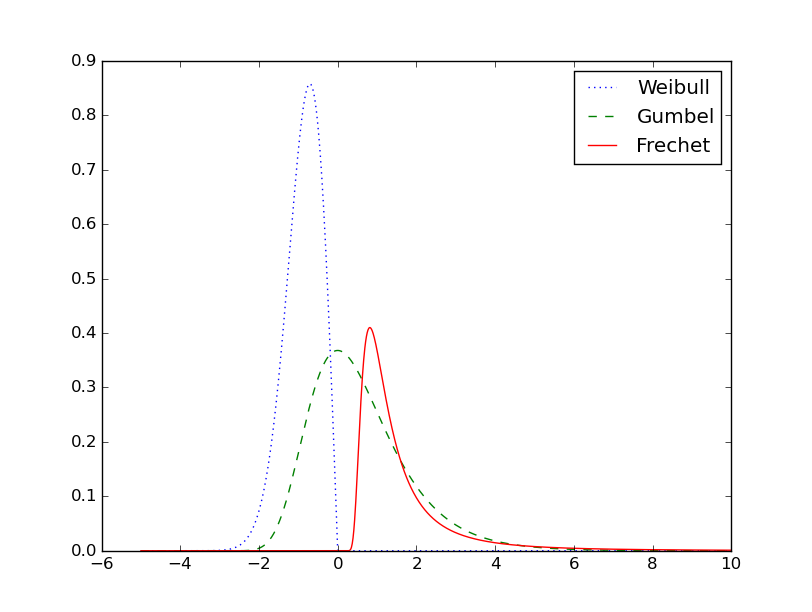
\includegraphics[width=.9\linewidth]{fig_source/GEV.png}
  \caption{Extreme Value Distribution with $\alpha = 2$}
  \label{fig:GEV}
\end{figure}

These extreme value distributions plotted in Figure~\ref{fig:GEV} can be summarized into the so-called Generalized Extreme Value (GEV) Distribution,
% $G(x) = \exp \left(-\left[1 + \gamma \frac{x-\mu}{\sigma}\right]^{-1/\gamma}\right),$
% defined on the set $\{x, 1+ \gamma \frac{x-\mu}{\sigma} > 0\}$ 
% or up to a re-scaling 
\begin{align}
\label{eq:GEV}
G(x) = \exp \left(-\left[1 + \gamma x\right]^{-1/\gamma}\right)
\end{align}
for $1 + \gamma x > 0$, $\gamma \in \mathbb{R}$,
setting by convention $(1 + \gamma x)^{-1/\gamma} = e^{-x}$ for
$\gamma = 0$ (continuous extension). % The sign of $\gamma$ controls the shape of the tail and
% various estimators of the re-scaling sequence and of the shape index $\gamma$ as well have
% been studied in great detail, see \emph{e.g.}  \cite{DEd1989},
% \cite{ELL2009}, 
% \cite{Hill1975}, \cite{Smith1987}, \cite{BVT1996}.
The sign of $\gamma$ controls the shape of the tail of $F$.
 In the case $\gamma >0$ (as for the Cauchy distribution), $G$ is referred to as a Fréchet distribution and $F$ has a heavy tail. If $\gamma=0$ (as for normal distributions), $G$ is a Gumbel distribution and $F$ has a light tail. If $\gamma < 0$ (as for uniform distributions), $G$ is called a Weibull distribution and $F$ has a finite endpoint.
Estimates of univariate extreme quantiles then rely on estimates of the parameters $a_n$, $b_n$, and $\gamma$, see \cite{DEd1989}, \cite{ELL2009}. 
The Hill estimator or one of its generalizations, see \cite{Hill1975, Smith1987, BVT1996, Girard2004, Boucheron2015}, provides an estimate of the tail parameter $\gamma$. 
%
A special case of extreme quantile estimation is when some covariate information is recorded simultaneously with the quantity of interest. The extreme quantile thus depends on the covariate and is called conditional extreme quantile \citep{Beirlant2004, Chernozhukov2005, Gardes2008, Gardes2010, Girard2008, Daouia2011, Daouia2013}.
%
\begin{example}
\begin{itemize}
\item Assume the $X_i$'s to be standard exponential variables (their cdf is $F(x) = 1 - e^{-x}$). In that case, letting $a_n=1$ and $b_n = \log(n)$, we have
$\mathbb{P}[(M_n-b_n)/a_n \le z] = \mathbb{P}[X_1 \le z + \log n ]^n = [1 - e^{-z}/n]^n \to \exp(-e^{-z}) $, for $z \in \rset$. The limit distribution is of Gumbel type ($\gamma = 0$).
\item If the $X_i$'s are standard Fréchet ($F(x) = \exp{(-1/z)}$), letting $an = n$ and $b_n = 0$, one has immediately $\mathbb{P}[(M_n-b_n)/a_n \le z] = F^n(nz) = \exp(-1/z)$, for $z >0$. The limit distribution remains the Fréchet one ($\gamma = 1$).
\item If the $X_i$'s are uniform on $[0,1]$, letting $a_n = 1/n$ and $b_n = 1$, one has $\mathbb{P}[(M_n-b_n)/a_n \le z] = F^n(n^{-1}z + 1) \to \exp(z)$, for $z <0$. The limit distribution is the Weibull one ($\gamma = -1$).

\end{itemize}
\end{example}

% Theorem~\ref{thm:univariate-evt} can be reformulated in the following way.
% Suppose there exists two
% sequences $\{a_n, n \ge 1\}$ and $\{b_n, n \ge 1\}$, the $a_n$'s being
% positive, and a non-degenerate distribution function $G$ such that
One can establish an equivalent formulation of Assumption~\eqref{eq:hyp-GEV} which does not rely anymore on the maximum $M_n$:
\begin{align}
\label{eq:hyp-GEV2} %instead of\label{intro:assumption1}
\lim_{n \to \infty} n ~\mathbb{P}\left( \frac{X - b_n}{a_n} ~\ge~ x \right) = -\log G(x)
\end{align}
for all continuity points $x \in \mathbb{R}$ of $G$.
The intuition behind this equivalence is that $$- \log(F^n(a_n x + b_n)) \sim n (1 - F(a_n x + b_n)) = n ~\mathbb{P}\left( \frac{X - b_n}{a_n}~\ge~ x \right)$$ when $n \to \infty$ as $F(a_n x + b_n) \sim 1$.
 The tail behavior of $F$
is then essentially characterized by $G$, which is proved to be -- up
to  re-scaling -- of the type~\eqref{eq:GEV}. 
\medskip
Note that Assumption~\eqref{eq:hyp-GEV} (or \eqref{eq:hyp-GEV2}) is fulfilled for most textbook distributions. In that case $F$ is said to lie in the \textit{domain of  attraction} of $G$, written $F \in DA(G)$.



%XXXXXXXXXXXXXXXXXXXXXXXXXXXXXXXXXXXXXXXXXXXXXXXXXXXXXXXXXXXXXXXXXXXXXXXXXXXXXXXXXXXXXXXXXXXXXXX
% Throughout this paper, for $a_j, b_j \in [0, \infty],~1 \le j \le d$ we use the notations $[a,b]=[a_1,b_1] \times ... \times[a_d,b_d]$ and for $T>0$, $0 \le x \le T$ means $0 \le x_1,...,x_d \le T$.
% Let $\mathbf{X_1,X_2,...,X_n}$ be iid random vectors in $\mathbb{R}^d$ with common distribution function $F$ and marginal distribution functions $F_1,...,F_d$.

\section{Extension to the Multivariate framework}
\label{back:sec:MEVT} 

Extensions to the multivariate setting are well understood
from a probabilistic point of view, but far from obvious from a
statistical perspective. Indeed, the tail dependence structure, ruling the possible simultaneous occurrence of large observations in several directions, has no finite-dimensional parametrization.

The analogue of Assumption (\ref{eq:hyp-GEV2}) for a $d$-dimensional \rv~$\mb X = (X^1,\; \ldots, \; X^d)$ with distribution $\mb F(\mb x):=\mathbb{P}(X_1 \le x_1, \ldots, X_d \le x_d)$, written $\mb F \in \textbf{DA} (\mb G)$ stipulates the existence of two sequences $\{\mb a_n, n \ge 1\}$ and $\{\mb b_n, n \ge 1\}$ in $\mathbb{R}^d$, the $\mb a_n$'s being positive,
and a non-degenerate distribution function $\mb G$ such that
\begin{align}
\label{eq:hyp-GEV2-mult}%\label{intro:assumption2}
\lim_{n \to \infty} n ~\mathbb{P}\left( \frac{X^1 - b_n^1}{a_n^1} ~\ge~ x_1 \text{~or~} \ldots \text{~or~} \frac{X^d - b_n^d}{a_n^d} ~\ge~ x_d \right) = -\log \mb G(\mathbf{x})
\end{align}
% \begin{align}
% \label{intro:assumption2}
% \lim_{n \to \infty} \mathbb{P}\left( \frac{\max_{1 \le i \le n} X_i^1 - b_n^1}{a_n^1} ~\le~ x_1, \ldots, \frac{\max_{1 \le i \le n} X_i^d - b_n^d}{a_n^d} ~\le~ x_d \right) =: G(x)
% \end{align}
for all continuity points $\mathbf{x} \in \mathbb{R}^d$ of $\mb G$. This clearly implies
that the margins $G_1(x_1),\ldots,G_d(x_d)$ are univariate extreme
value distributions, namely of the type $G_j(x) = \exp(-(1 + \gamma_j
x)^{-1/\gamma_j})$. Also, denoting by $F_1,\; \ldots,\; F_d$ the
marginal
distributions of $\mb F$, Assumption~\eqref{eq:hyp-GEV2-mult} implies marginal convergence: $F_i \in DA(G_i)$ for $i=1,\; \ldots,\; n$.
 To understand %capture 
the structure of the limit $\mb G$ and dispose of the
 unknown sequences $(\mb a_n, \mb b_n)$ (which are entirely determined by the
 marginal distributions $F_j$'s), % It is  mathematically very convenient to decompose the joint distribution of $\mb X = (X^1,\ldots, X^d)$ into the margins on the one hand, and the dependence structure on the other hand.
 it is convenient to
 work with marginally standardized variables, that is, to separate the margins from the dependence structure in the description of the joint distribution of $\mb X$. Consider the standardized variables 
 $V^j =1/(1-F_j(X^j))$ and $\mathbf{V}=(V^1,\; \ldots,\; V^d)$.  In
 fact (see Proposition 5.10 in \cite{Resnick1987}), Assumption~\eqref{eq:hyp-GEV2-mult} is
 equivalent to:

\begin{itemize}
\item  marginal convergences $F_j \in DA(G_j)$ as in (\ref{eq:hyp-GEV2}),  % of the marginal distributions \ie~$F_i \in DA(G_i)$, $i=1,\ldots,n$,
 together with 
\item standard  multivariate regular variation of $\mathbf{V}$'s
 distribution,  which means existence of a limit measure $\mu$  on $ [0,\infty]^d\setminus\{\mb 0\}$ such that % convergence of
\begin{align}
\label{back:intro:regvar}
 n~ \mathbb{P}\left( \frac{V^1 }{n} ~\ge~ v_1 \text{~or~} \cdots
   \text{~or~} \frac{V^d }{n} ~\ge~ v_d \right) \xrightarrow[n\to\infty]{}\mu \left([\mb 0,\mb v]^c\right),
\end{align}
where $[\mb 0,\mathbf{v}]:=[0,\; v_1]\times \cdots \times
[0,\; v_d]$.
\end{itemize}

 Thus the variable $\mb V$ satisfies
(\ref{eq:hyp-GEV2-mult}) with $\mb a_n = \mb n = (n,\; \ldots,\; n)$, $\mb b_n =\mb 0 =(0,\; \ldots,\; 0)$. 

\begin{remark} %XXX to be verified
The standardization in $V$ allows to study the same extreme value distribution for each marginal, and with the same re-scaling sequences $a_n$ and $b_n$ for each marginal. In the case of Pareto standardization like here, the underlying extreme value distribution is the Fréchet one.
\end{remark}

The dependence structure of the limit $\mb G$ in (\ref{eq:hyp-GEV2-mult})
can be expressed by means of the so-termed \textit{exponent measure} $\mu$: 
\begin{align}
- \log \mb G(\mathbf{x})= \mu\left( \left[ \mb 0, \left(\frac{-1}{\log G_1(x_1)}, \dots ,\frac{-1}{\log G_d(x_d)}\right)\right]^c\right). \nonumber
\end{align}
The latter  is finite on
sets bounded away from $\mb 0$ and has the
homogeneity property : $\mu(t\point) =
t^{-1}\mu(\point)$. Observe in addition that, due to the standardization chosen (with
`nearly' Pareto margins), the support of $\mu$ is included in $[\mb 0,\; \mathbf{1}]^c$. % then be written using the stable
% tail dependence function ({\sc stdf}) $l$ :
% \begin{align*}
% G(\mathbf{x})=\exp (~ -l(-\log G_1(x_1), \dots ,-\log G_d(x_d)~ )
% \end{align*}
%The so-called \emph{exponent measure} $\mu$ is finite on
%sets bounded away from $0$ and has the
%homogeneity property : $\mu(t\point) =
%t^{-1}\mu(\point)$. Further, due to our standardization choice to
%`nearly' Pareto margins, it can be shown that 
%\begin{align}
 % \label{eq:normalizing_mu_vj_ge1}
 % \mu\{\mb v~:v_j>1\} = 1\;;\qquad j=1\,\ldots,d.
%\end{align}
 To wit, the measure $\mu$ should be viewed, up to a a normalizing factor, as
the asymptotic distribution of $\mb V$ in extreme regions. For any borelian subset $A$ bounded away from $\mb 0$ on which $\mu$ is continuous, we have 
\begin{align}
\label{eq:regularVariation}
t~ \mathbb{P}\left( \mb V \in t A\right) \xrightarrow[t\to\infty]{}\mu(A).     
\end{align}
Using the homogeneity property $\mu(t\point) =
t^{-1}\mu(\point)$, one may show
that $\mu$  can be decomposed into a  radial component and an angular component
$\Phi$, which are independent from each other (see \emph{e.g.} \cite{dR1977}).
Indeed, for all $\mb v = (v_1,...,v_d) \in \mathbb{R}^d$, set
\begin{align}\label{eq:pseudoPolar_change}
  \left\{ \begin{aligned}
R(\mb v)&:= \|\mb v\|_\infty ~=~ \max_{i=1}^d v_i, \\
\Theta (\mb v) &:= \left( \frac{v_1}{R(\mb v)},..., \frac{v_d}{R(\mb v)} \right)
\in S_\infty^{d-1},     
  \end{aligned}\right.
\end{align}
where $S_\infty^{d-1}$ is the positive orthant of  the unit sphere in $\mathbb{R}^d$ for the infinity norm.
Define the \emph{ spectral measure} (also called \emph{angular measure}) by $\Phi(B)= \mu (\{\mb v~:~R(\mb v)>1 ,
\Theta(\mb v) \in B \})$. Then, for every $B
\subset S_\infty^{d-1}$, 
\begin{align}
\label{mu-phi}
\mu\{\mb v~:~R(\mb v)>z, \Theta(\mb v) \in B \} = z^{-1} \Phi (B)~. 
\end{align}
In a nutshell,  there
is a one-to-one correspondence between the exponent measure $\mu$ and the angular measure
$\Phi$, both of them can be used to characterize the asymptotic tail
dependence of the distribution $\mb F$ (as
soon as the  margins $F_j$ are known), since   % after each marginal had been standardized in $\mathbf{U}$ or $\mathbf{V}$.
\begin{align}\label{eq:integratePhiLambda}
  \mu \big( [\mb 0,\mathbf{x}^{-1}]^c \big) =  \int_{\boldsymbol{\theta} \in S_{\infty}^{d-1}}   \max_j{\boldsymbol{\theta}_j x_j} \;\ud \Phi(\boldsymbol{\theta}),
\end{align}
%where $S^{d-1}:= \{w \in [0,1]^d, w_1+\ldots w_d =1\}$, and 
this equality being obtained from the change of variable~\eqref{eq:pseudoPolar_change} , see \emph{e.g.} Proposition 5.11 in \cite{Resnick1987}. 
Recall that here and beyond, operators on vectors are understood component-wise, so that $\mb x^{-1}=(x_1^{-1},\ldots,x_d^{_1})$.
The angular measure can be seen as the asymptotic conditional distribution of the
`angle' $\Theta$ given that the radius $R$ is large, up to the
normalizing constant $\Phi(S_\infty^{d-1})$. Indeed, dropping
the dependence on $\mb V$ for convenience, we have for any
\emph{continuity set} $A$ of $\Phi$, 
\begin{align}
  \label{eq:limitConditAngle}
\begin{aligned}
  \PP(\Theta \in A ~|~R>r ) &= 
\frac{r  \PP(\Theta \in A , R>r ) }{r\PP(R>r)} 
& \xrightarrow[r\to \infty]{} \frac{\Phi(A)}{\Phi(S_\infty^{d-1})} .
\end{aligned}  
\end{align}
The choice of the marginal standardization is somewhat arbitrary and alternative standardizations  lead
to different limits. Another common choice consists in considering `nearly
uniform' 
variables (namely, uniform variables when the margins are continuous): defining $\mathbf{U}$ by $U^j =1-F_j(X^j)$ for
$j\in\{1,\ldots,d\}$,   % the existence of the limit in (\ref{eq:hyp-GEV2-mult}) is then equivalent to each
% of the following conditions (with the notations $\mathbf{x}^{-1}=(x_1^{-1},\ldots,x_d^{-1})$ and $[0,\mathbf{x}]=[0,x_1]\times \ldots \times [0,x_d]$) :
condition (\ref{back:intro:regvar}) is equivalent to each of the  following conditions:
\begin{itemize}
\item $\mathbf{U}$ has  `inverse multivariate regular variation' % on $[0,\infty]^d \setminus \{\infty\}$
  with limit measure $\Lambda(\point)$ $:=\mu((\point)^{-1})$, namely,
  for every measurable set $A$ bounded away from $+\boldsymbol{\infty}$ which is a
  continuity set of $\Lambda$,
\begin{align}
\label{back:reg_var_U}
t~ \mathbb{P}\left( \mb U \in t^{-1} A\right)
\xrightarrow[t\to\infty]{} \Lambda(A) = \mu(A^{-1}), 
\end{align}
where $A^{-1} = \{\mb u \in \rset^{d}_+ ~:~(u_1^{-1},\ldots,u_d^{-1})
\in A\}$. The limit measure $\Lambda$ is finite on sets bounded away from $\{+\boldsymbol{\infty}\}$. 
\item The \textit{stable tail dependence function} (\stdf) defined for $\mb x\in[\mb 0,\boldsymbol{\infty}], \mb x\neq\boldsymbol{\infty}$ by 
\begin{align}
\label{back:stdf1}
l(\mb x) = \lim_{t \to 0} t^{-1} \mathbb{P} \left( U^1 \le t\, x_1 ~\text{or}~ \ldots ~\text{or}~ U^d \le t\,x_d  \right)
 = \mu\left([\mb 0, \mb{x}^{-1}]^c\right) 
\end{align}
exists. 
\end{itemize}

As a conclusion, in multivariate extremes, the focus is on the dependence structure which is characterized by different quantities, such as the exponent measure $\mu$ (itself characterized by its angular part $\Phi$) or the \stdf, which is closely linked to other integrated version of $\mu$ such as extreme-value copula or tail copula. For details on such 
functionals, see~\cite{Segers12}.
The fact that these quantities characterize the dependence structure can be illustrated by the link they exhibit between the multivariate GEV $G(x)$ and the marginal ones $G_j(x_j),~1 \le j \le d$,

\begin{align*}
- \log \mb G(\mathbf{x})~&=~ \mu\left( \left[ \mb 0, \left(\frac{-1}{\log G_1(x_1)}, \dots ,\frac{-1}{\log G_d(x_d)}\right)\right]^c\right) ~~~~~\text{for the exponent measure,}\\
 - \log \mb G(\mb x) ~&=~ l(-\log G_1(x_1), \ldots, -\log G_d(x_d)) ~~~~~~~~~~~~~~~~~~~~ \text{for the \stdf,}\\
 G( \mb x) ~&=~ C(G_1(x_1), \ldots, G_d(x_d)) ~~~~~~~~~~~~~~~~~~~~~~~~~~~~~~~~~~~~~ \text{for the extreme value copula } C.
\end{align*}


In Chapter~\ref{colt}, we develop non-asymptotic bounds for non-parametric estimation of the \stdf.
As in many applications, it can be more convenient to work with the angular measure itself -- the latter gives more direct information on the dependence structure --, Chapter~\ref{jmva} generalizes the study in Chapter~\ref{colt} to the angular measure.


%XXX commments on these assumptions
% \begin{assumption}\label{hypo:M}
% For every $\beta$ such that $|\beta| > 2$,~ $M_\beta$ is finite and $|\beta_1| \le |\beta_2| \Rightarrow M_{\beta_1} \ge M_{\beta_2}$.
% \end{assumption}
% One 'parcimony assumption' would be something like $M_\beta\le e^{-|\beta|}$.

% In other words we select, for each feature $j\le d$, the `$k$ largest values' $X_i^j$
% over the $n$ observations. According to the nature of the extremal dependence,
% a number between $k$ and $dk$ of observations are selected: $k$ in
% case of perfect dependence, $dk$ in case of `asymptotic independence', which
% means, in EVT, that the components may only be large one at a time. In
% any case, the number of observations considered as extreme is proportionnal to $k$, whence the normalizing factor $\frac{n}{k}$. 

%


% Yet the goal is to study the dependence between the $V_i^j$, $i$ fixed anf $j$ varying.
% One way to proceed is to characterize, for each subset of features
% $\alpha \subset \{1,...,d\}$, the `correlation' of these features
% given that one of them at least  is large and the others are small. %extreme (\ie~given that the observation is extreme).
% Formally, we  associate to each such $\alpha$ a coefficient
% $\mu_n^\alpha$ reflecting the degree of dependence between the
% features $\alpha$. Theoretically, by definition of asymptotic
% dependence, this coeficient is to be proportional to the expected number of
% points $V$ verifying $V^j > 0$, $j \in \alpha$ and $V^j = 0,~ j\notin
% \alpha$, and $\|V\|_\infty\ge r$, namely $ r^{-1}V \in \mathcal{C}_\alpha$ with 
% \begin{align}
% %\label{cone}
% \mathcal{C}_\alpha = \{v \ge 0,~\|v\|_\infty \ge 1,~ v_j > 0 ~\text{ for } j \in \alpha,~ v_j = 0 ~\text{ for } j \notin \alpha \}.
% \end{align}
% (see Fig.~\ref{fig:3Dcones}) But in practice, the data are non-asymptotic so that if $\alpha \neq \{1,\ldots,d\}$ the cones $\mathcal{C}_\alpha$ have zero Lebesgue measure and are not likely to receive empirical mass. Consider then a tolerance parameter $\epsilon>0$ and approximate the asymptotic mass of $~\mathcal{C}_\alpha~$ by the non-asymptotic mass of 
% \begin{align}
%  \label{eq:epsilonCone}
%  ~\mathcal{C}_\alpha^\epsilon~=\{v \ge
%  0,~\|v\|_\infty \ge 1,~ v_j > \epsilon \|v\|_\infty ~\text{ for } j
%  \in \alpha,~v_j \le \epsilon\|v\|_\infty ~\text{ for } j \notin \alpha
%  \} ,
% \end{align}
% which leads to coefficients 

% This motivates the study of the STDF $l$, since it is now theoretically clear how the asymptotic tail dependence structure of $F$ is contained in $l$.
% XXXXXXXXXXXXXXXXXXXXXXXXXXXXXXXXXXXXXXXXXXXXXXXXXXXXXXXXXXXXXXXXXXXXXXXXXXXXXXXXXXXXXXXXXXXXXXXX
% % The measures $\mu$ and $\Lambda$ are called exponent measures and have the following properties:
% % \begin{itemize}
% % \item standardized marginals: for all $a>0$,
% % \begin{align*}
% % \Lambda([0,a]\times[0,\infty]^{d-1})~=~\Lambda([0,\infty]&\times[0,a]\times[0,\infty]^{d-2})
% % \\&~=~...~=~\Lambda([0,\infty]^{d-1}\times[0,a])~=~a
% % \end{align*}
% % \noindent and
% % \begin{align*} 
% % \mu([a,\infty]\times[0,\infty]^{d-1})~=~\mu([0,\infty]&\times[a,\infty]\times[0,\infty]^{d-2})
% % \\&~=~...~=~\mu([0,\infty]^{d-1}\times[a,\infty])~=~a^{-1}
% % \end{align*}
% % \item homogeneity: $\Lambda(c.)=c~ \Lambda(.)$ and $\mu(c.)=c^{-1} \mu(.)$
% % \item concentration: $\Lambda$, $\mu$ are respectively concentrated on $(0,\infty]^d \setminus \{\infty\}$, $[0,\infty)^d \setminus \{0\}$
% % \end{itemize}
% The homogeneity property yields a decomposition of $\mu$ into a
% radial and angular part (see de Haan and Resnick ...). 


\chapter{Background on classical Anomaly Detection algorithms}
\label{back:AD_scikit}
\begin{chapabstract}
  In this chapter, we review some very classical anomaly detection algorithms used in the benchmarks of chapters~\ref{chap:ocrf} and \ref{chap:evaluation}. We also introduce the reader to the scikit-learn library used for illustrative examples, and present relative (implementative) contributions of this thesis. %This is also the opportunity to present implementative contributions of this thesis, as two of the algorithms presented here, the Isolation Forest algorithm (Section \ref{sec:iforest}) and the Local Outlier Factor algorithm (Section \ref{sec:lof}), have been implemented on scikit-learn in the context of this Ph.D., as mentioned in the introduction.
\end{chapabstract}

Note: The work on scikit-learn was supervised by Alexandre Gramfort and is the result of a collaboration with the Paris Saclay Center for Data Science. It includes the implementation of Isolation Forest (Section \ref{sec:iforest}) and Local Outlier Factor (Section \ref{sec:lof}) algorithms, as well as a participation to the scikit-learn maintenance and pull requests review.


\section{What is Anomaly Detection?}
Anomaly Detection % (and depending on the application domain, outlier detection, novelty detection, deviation detection, exception mining)
generally consists in assuming that the dataset under study contains a \textit{small} number of anomalies, generated by distribution models that  \textit{differ} from the one generating the vast majority of the data.
 % anomalies are a \textit{small} number of observations generated by \textit{different} models from the one generating the rest of the data
%\sout{ -- the only difference in novelty detection is that the novel patterns are incorporated into the normal model after being detected. }.
This formulation motivates many statistical anomaly detection methods, based on the underlying assumption that anomalies occur in low probability regions of the data generating process. Here and hereafter, the term `normal data' does not refer to Gaussian distributed data, but to \emph{not abnormal} ones, \ie~data belonging to the above mentioned majority. We also call them sometimes \emph{inliers}, while abnormal data are called \emph{outliers}. 
Classical parametric techniques, like those developed by \cite{Barnett94} and \cite{Eskin2000}, assume that the normal data are generated by a distribution belonging to some  specific, known in advance parametric model.  
The most popular non-parametric approaches include algorithms based on density (level set) estimation \citep{Breunig2000LOF, Scholkopf2001, Steinwart2005, Scott2006, VertVert}, on dimensionality reduction \citep{Shyu2003, Aggarwal2001} or on decision trees \citep{Liu2008, Desir12, Shi2012}.
% %approach is statistical, \
% % {\red donner le theme de chaque papier cité}
% \cite{Eskin2000},
% \cite{Desforges1998}, \cite{Barnett94}, \cite{Hawkins1980}
% , distance
% based, \cite{Knorr98}, \cite{Knorr2000}, \cite{Eskin2002geometric},
% local-density based \cite{Breunig2000LOF}, \cite{Breunig99LOF},
% \cite{Tang2002enhancing}, \cite{Papadimitriou2003loci}, spectral based
% \cite{Shyu2003}, \cite{Wang2006}, \cite{Lee2013} and others
% \cite{Aggarwal2001}, \cite{Kriegel2008}, \cite{Liu2008}. 
One may refer to \cite{Hodge2004survey, Chandola2009survey, Patcha2007survey, Markou2003survey} for overviews of current research on Anomaly Detection, ad-hoc techniques being far too numerous to be listed here in an exhaustive manner.


 Most usual anomaly detection algorithms actually
provide more than a predicted label for any new observation, abnormal/normal. Instead,
they return a real valued function,  termed a \textit{scoring function}, defining a pre-order/ranking on the input space. Such a function permits to rank any observations according to their supposed `degree of abnormality' and thresholding it yields a decision rule that splits the input space into `normal' and `abnormal' regions.
In various fields (\textit{e.g.} fleet management, monitoring of energy/transportation networks), when confronted with massive data, being able to rank observations according to their degree of abnormality may significantly improve operational processes and allow for a prioritization of actions to be taken, especially in situations where human expertise is required to check each observation is time-consuming.


From a machine learning perspective, anomaly detection can be considered as a specific classification/ranking task, where the usual assumption in supervised learning stipulating that the dataset contains structural information regarding all classes breaks down, see \cite{Roberts99}. This typically happens in the case of two highly unbalanced classes: the normal class is expected to regroup a large majority of the dataset, so that the very small number of points representing the abnormal class does not allow to learn information about this class.
In a clustering based approach, it can be
interpreted as the presence of a single cluster, corresponding to the
normal data. The abnormal ones are too limited to share a common
structure, \ie~to form a second cluster. Their only characteristic is
precisely to lie outside the normal cluster, namely to lack any
structure.  Thus, common classification approaches may not be applied
as such, even in a supervised
context. % That is the reason why even in a supervised framework, common classification approaches cannot be applied.
\textbf{Supervised} anomaly detection consists in training the algorithm on a labeled (normal/abnormal) dataset including both normal and abnormal observations. In the \textbf{novelty detection} framework (also called \emph{one-class classification} or \emph{semi-supervised} anomaly detection), only normal data are available for training. This is the case in applications where normal operations are known but intrusion/attacks/viruses are unknown and should be detected. In the \textbf{unsupervised} setup (also called \emph{outlier detection}), no assumption is made on the data which consist in unlabeled normal and abnormal instances. In general, a method from the novelty detection framework may apply to the unsupervised one, as soon as the number of anomalies is sufficiently weak to prevent the algorithm from fitting them when learning the normal behavior. Such a method should be robust to outlying observations.

Let us also mention the so-called \emph{semi-supervised novelty detection} \citep{Blanchard2010, Smola2009} framework which is closely linked to the \emph{PU learning framework} \citep{Denis2005, Liu2002, Mordelet2014, duPlessis2015}. 
Semi-supervised novelty detection consists in learning from negative and unsupervised examples, while PU learning consists in learning from positive (P) and unlabeled (U) examples. These hybrid approaches assume that both an unlabeled sample and a sample from one class are available.

In this thesis, we basically place ourselves in the novelty detection framework, although some benchmarks are also done on (unlabeled) training data polluted by outliers, namely in the unsupervised framework.

\section{Three efficient Anomaly Detection Algorithms}
\label{sec:AD_sklearn}


\subsection{One-class SVM}
\label{back:ocsvm}
The SVM algorithm is essentially a two-class algorithm (\ie~one needs negative as well as positive examples).
\cite{Scholkopf2001} extended the SVM methodology to handle training using only positive information:
the One-Class Support Vector Machine (OCSVM) treats the origin as the only member of the second class (after mapping the data to some feature space). Thus the OCSVM finds a separating hyperplane between the origin and the mapped one class. %, using some `relaxation parameters'.

The OCSVM consists in estimating Minimum Volume sets, which amounts (if the density has no flat parts) to estimating density level sets, as mentioned in the introduction.
In \cite{VertVert}, it is shown that the OCSVM is a consistent estimator of density level sets, and that the solution function returned by the OCSVM gives an estimate of the tail of the underlying density.

%
% As a good sketch is better than a long speech, we refer to 
Figures~\ref{table:OCSVM-hard} and \ref{table:OCSVM-soft}  summarizes the theoretical insights of OCSVM compared to the standard SVM, respectively for the hard-margin (no error is tolerated during training) and soft-margin separation (some margin errors are tolerated in training).
\renewcommand{\arraystretch}{1.5}
\begin{table}[!ht]
  \caption{SVM vs. OCSVM (hard-margin separation)}
  \label{table:OCSVM-hard}
  \centering
\resizebox{\linewidth}{!} {
  \begin{tabular}{cc}\toprule
    SVM                                                             &    OCSVM  \\ \midrule 
    $\displaystyle \min_{w,b} \frac{1}{2} \|w\|^2$                   & $\displaystyle \min_{w} \frac{1}{2} \|w\|^2$   \\
    s.t~~~~ $\forall i,~~y_i(\langle w, x_i\rangle + b) \ge 1$      & s.t~~~~ $\forall i,~~\langle w, x_i\rangle ~\ge 1$ \\ \midrule %\cdashline{1-2}
    \multicolumn{2}{l}{~}\\
    \multicolumn{2}{l}{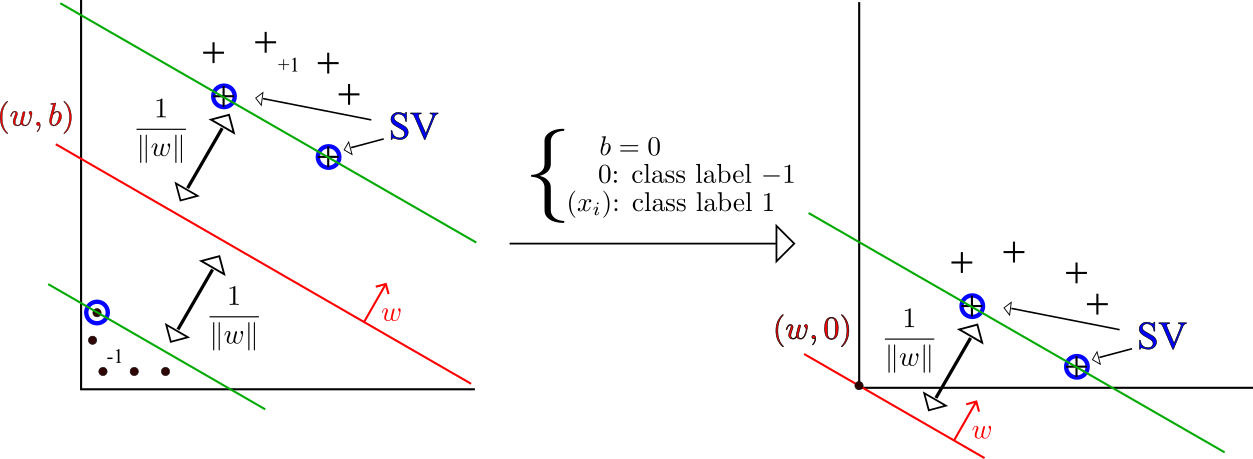
\includegraphics[scale=0.83]{fig_source/OCSVM_hard}} \\\midrule %\cdashline{1-2}
    decision function:                                             & decision function:  \\
    ~~~~~~~~$f(x) = \text{sgn}(\langle w, x\rangle + b)$ ({\red red line}) ~~~~~~~ & $f(x) = \text{sgn}(\langle w, x\rangle - 1)$ ({\green green line}) \\ \midrule %\cdashline{1-2} 
    \multicolumn{2}{l}{-Lagrange multipliers: $\alpha_i$ ~~~~($\alpha_i>0$ when the constraint is an equality for $x_i$)} \\
    \multicolumn{2}{l}{-Support vectors: $\text{SV} = \{ x_i,~~ \alpha_i > 0\}$ }\\
    \multicolumn{2}{l}{-Margin errors: $\text{ME} = \emptyset $ ~~~~~~~~~~~~~~~ }\\\midrule % \cdashline{1-2}
    $\displaystyle w = \sum_i \alpha_i y_i x_i$                    & $\displaystyle w = \sum_i \alpha_i x_i$  \\ \bottomrule
  \end{tabular}
}
\end{table}

\begin{table}[!ht]
  \caption{SVM vs. OCSVM ($\nu$-soft margin separation)}
  \label{table:OCSVM-soft}
  \centering
\resizebox{\linewidth}{!} {
  \begin{tabular}{cc}\toprule
    SVM                                                             &    OCSVM  \\ \midrule 
    $\displaystyle \min_{w,\xi,\rho,b} \frac{1}{2} \|w\|^2 + \frac{1}{n} \sum_{i=1}^n \xi_i - \nu \rho$ & $\displaystyle \min_{w,\xi,\rho} \frac{1}{2} \|w\|^2 + \frac{1}{n} \sum_{i=1}^n \xi_i - \nu \rho$  \\
    s.t~~~~ $\forall i, ~~y_i(\langle w, x_i\rangle ~+~ b) \ge \rho - \xi_i$                        & s.t~~~~ $\forall i,~~\langle w, x_i\rangle ~\ge \rho - \xi_i $ ~~~~~~\\ 
    $\xi_i \ge 0$ ~~~~~~~~~~~~~~~~~~~~~                                                            & $\xi_i \ge 0$~~~~~~~~~~~~  \\ \midrule % \cdashline{1-2}
    \multicolumn{2}{l}{~}\\
    \multicolumn{2}{l}{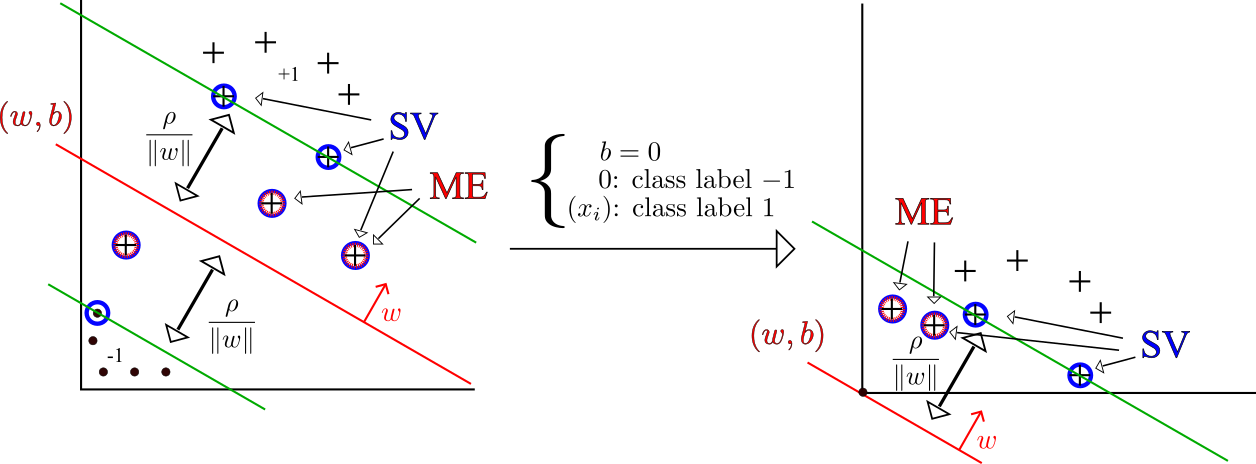
\includegraphics[scale=0.83]{fig_source/OCSVM_soft}} \\\midrule %\cdashline{1-2}
    decision function:                                                                             & decision function:  \\
    ~~~~~~~~$f(x) = \text{sgn}(\langle w, x\rangle + b)$ ({\red red line}) ~~~~~~~            & $f(x) = \text{sgn}(\langle w, x\rangle - \rho)$ ({\green green line})\\ \midrule % \cdashline{1-2}
    \multicolumn{2}{l}{-Lagrange multipliers: $\alpha_i, \beta_i$ ~~~~(one for each constraint, $\beta_i > 0$ when $\xi_i = 0$)}\\
    \multicolumn{2}{l}{-Support vectors: $\text{SV} = \{ x_i,~~ \alpha_i > 0\}$ }\\
    \multicolumn{2}{l}{-Margin errors: $\text{ME} = \{x_i,~~ \xi_i > 0 \} =  \{x_i,~~ \beta_i > 0 \} $ ~~~(for OCSVM, ME=anomalies) }\\
    \multicolumn{2}{l}{-$\text{SV} \setminus \text{ME} = \{ x_i,~~ \alpha_i, \beta_i > 0\}$ }\\ \midrule % \cdashline{1-2}
    $w = \sum_i \alpha_i y_i x_i$                                                                   & $w = \sum_i \alpha_i x_i$  \\ \midrule % \cdashline{1-2}
    \multicolumn{2}{c}{ $\displaystyle \frac{|\text{ME}|}{n} ~\le~ \nu ~\le~ \frac{|\text{SV}|}{n}$ }   \\
    \multicolumn{2}{c}{$\displaystyle \rho = \langle w, x_i\rangle ~~~~\forall x_i \in \text{SV} \setminus \text{ME}$} \\ \bottomrule %\hline
  \end{tabular}
}
\end{table}
\renewcommand{\arraystretch}{1.1}

In the $\nu$-soft margin separation framework, letting $\Phi$ be the mapping function determined by a kernel function $k$ (\ie~$k(x,y) = \langle \Phi(x), \Phi(y)\rangle$), the separating hyperplane defined \wrt~a vector $w$ and an offset $\rho$ is given by the solution of 
\begin{align*}
&\min_{w,\xi,\rho} \frac{1}{2} \|w\|^2 + \frac{1}{n} \sum_{i=1}^n \xi_i - \nu \rho\\
&\text{s.t.}~~~ \langle w, \Phi(x_i)\rangle ~\ge \rho - \xi_i~~,~~~~~~1 \le i \le n \\
& ~~~~~~~~\xi_i \ge 0,
\end{align*}
where $\nu$ is previously set. An interesting fact is that $\nu$ is an upper bound on the fraction of outliers and a lower bound on the fraction of support vectors, both of which converging to $\nu$ almost surely as $n \to \infty$ (under some continuity assumption). Then, the empirical mass of the estimated level set is greater than $1-\nu$ and converges almost surely to $1-\nu$ as $n$ tends to infinity. Hence one usual approach is to choose $\nu = 1 - \alpha$ to estimate a MV-set with mass (at least) $\alpha$. For insights on the calibration of One-Class SVM, see for instance \cite{Thomas2015}.
%
The OCSVM is mainly applied with Gaussian kernels and its performance highly depends on the kernel bandwidth selection.
The complexity of OCSVM training is the same as for the standard SVM, namely $O(n^3 d)$ where $n$ is the number of samples and $d$ the dimension of the input space. However, one can often expect a complexity of $O(n^2 d)$, see \cite{Bottou2007}. From its linear complexity \wrt~the number of features $d$, OCSVM scales well in large dimension, and performance remains good even when the dimension is greater than $n$. By using only a small subset of the training dataset (support vectors) in the decision function, it is memory efficient. However, OCSVM suffers from practical limitation: 1) the non-linear training complexity in the number of observations, which limits its use on very large datasets; 2) its sensitivity to the parameter $\nu$ and to the kernel bandwidth, which makes calibration tricky; 3) parametrization of the mass of the MV set estimated by the OCSVM via the parameter $\nu$ does not allow to obtain nested set estimates as the mass $\alpha$ increases.

\subsection{Local Outlier Factor algorithm}
\label{sec:lof}
One other very efficient way of performing outlier detection in datasets whose dimension is moderately large is to use the Local Outlier Factor (LOF) algorithm proposed in \cite{Breunig2000LOF}.

This algorithm computes a score reflecting the degree of abnormality of the observations, the so-called local outlier factor. It measures the local deviation of a given data point with respect to its neighbors. By comparing the local density near a sample to the local densities of its neighbors, one can identify points which have a substantially lower density than their neighbors. These are considered to be outliers.

In practice the local density is obtained from the $k$-nearest neighbors. The LOF score of an observation is equal to the ratio of the average local density of his $k$-nearest neighbors, and his own local density: a normal instance is expected to have a local density similar to that of its neighbors, while abnormal data are expected to have much smaller local density.

The strength of the LOF algorithm is that it takes both local and global properties of datasets into consideration: it can perform well even in datasets where abnormal samples have different underlying densities. The question is not, how isolated the sample is, but how isolated it is with respect to the surrounding neighborhood.


\subsection{Isolation Forest}
\label{sec:iforest}


One efficient way of performing outlier detection in high-dimensional datasets
is to use random forests.
%
The IsolationForest proposed in \cite{Liu2008} 'isolates' observations by randomly selecting a feature and then randomly selecting a split value between the maximum and minimum values of the selected feature.
%
Since recursive partitioning can be represented by a tree structure, the
number of splittings required to isolate a sample is equivalent to the path
length from the root node to the terminating node.
%
This path length, averaged over a forest of such random trees, is a measure
of abnormality. The scoring function is based on this averaged depth.
%
Random partitioning produces noticeable shorter paths for anomalies, see figures~\ref{fig:ideeIF} and \ref{fig:convergenceIF}. Moreover, the average depth of a sample over the forest seems to converge to some limits, the latter being different whether the sample is or not an anomaly.
Hence, when a forest of random trees collectively produces shorter path lengths
for particular samples, they are highly likely to be anomalies.
%




\section{Examples through scikit-learn}
\label{back:sklearn-contribution}
This section provides examples on the anomaly detection algorithms presented above through the scikit-learn python library.

As mentioned in the introduction, contribution of this thesis includes the implemention of two classical anomaly detection algorithms on the open-source scikit-learn library (\cite{sklearn2011}), namely the Isolation Forest algorithm (\cite{Liu2008}) and the Local Outlier Factor algorithm (\cite{Breunig2000LOF}). % , which are respectively presented in sections \ref{sec:lof} and \ref{sec:iforest}.
This work was supervised by Alexandre Gramfort and is the result of a collaboration with the Paris Saclay Center for Data Science. It also includes participation to the scikit-learn maintenance and pull requests review.

% by describing and comparing anomaly detection algorithms from this library. Part of this section are modified versions of the documentation included in the forementioned scikit-learn contribution.


\subsection{What is scikit-learn?}
Scikit-learn, see \cite{sklearn2011}, is an open-source library which provides well-established machine learning methods.
It is a Python module, the latter language being very popular for scientific computing, thanks to its high-level interactive nature. Python is enjoying this recent years a strong expansion both in academic and industrial settings. Scikit-learn takes advantage of this favorable backdrop and extends this general-purpose programming language with machine learning operation: It not only provides implementations of many established algorithms, both supervised and unsupervised, while keeping an easy-to-use interface tightly integrated with the Python language. But it also provides a composition mechanism (through a \emph{Pipeline} object) to combine estimators, preprocessing tools and model selection methods in such a way that the user can easily construct complex ad-hoc algorithms.

Scikit-learn depends only on \emph{numpy} (the base data structure used for data and model parameters, see \cite{Vanderwalt2011numpy}) and \emph{scipy} (to handle common numerical operations, see \cite{Jones2015scipy}).
Most of the Scikit-learn package is written in python and \emph{cython}, a compiled programming language for combining C in Python to achieve the performance of C with high-level programming in Python-like syntax.


The development is done on \emph{github}\footnote{https://github.com/scikit-learn}, a Git repository hosting service which facilitates collaboration, as coding is done in strong interaction with other developers. Because of the large number them, emphasis is put on keeping the project maintainable, \eg~by avoiding duplicating code.% up to pay (reasonably) in computational performance. As an example, the initial Isolation Forest implementation contained a complementary cython code to efficiently browse the trees of the forest. This functionality was included in an other (more complete) tree browser, but which is heavier in terms of computation. A balance had to be made between the computational gain and the maintainability cost, which led to choose the last one.


Scikit-learn benefits from a simple and consistent API (Application Programming Interface), see \cite{sklearn_api2013}, through the \emph{estimator} interface. This interface is followed by all (supervised and unsupervised) learning algorithms as well as other tasks such as preprocessing, feature extraction and selection. The central object \emph{estimator} implements a \emph{fit} method to learn from training data, taking as argument an input data array (and optionally an array of labels for supervised problems). The initialization of the estimator is done separately, before training, in such a way the constructor doesn't see any data and can be seen as a function taking as input the model hyper-parameters and returning the learning algorithm initialized with these parameters. Relevant default parameters are provided for each algorithm. To illustrate initialization and fit steps, the snippet below considers an anomaly detection learning task with the \emph{Isolation Forest} algorithm.

\begin{pythoncode} 
# Import the IsolationForest algorithm from the ensemble module
from sklearn.ensemble import IsolationForest

# Instantiate with specified hyper-parameters
IF = IsolationForest(n_trees=100, max_samples=256)

# Fit the model on training data (build the trees of the forest)
IF.fit(X_train)
\end{pythoncode}


In this code example, the Isolation Forest algorithm is imported from the \emph{ensemble} module of scikit-learn, which contains the ensemble-based estimators such as bagging or boosting methods. Then, an $IsolationForest$ instance $IF$ is initialized with a number of trees of $100$ (see Section~\ref{sec:iforest} for details on this algorithm). Finally, the model is learned from training data $X\_train$ and stored on the $IF$ object for later use. Since all estimators share the same API, it is possible to train a Local Outlier Factor algorithm by simply replacing the constructor name $IsolationForest(n\_trees=100)$ in the snippet above by $LocalOutlierFactor()$.

Some estimators (such as supervised estimators or some of the unsupervised ones, like Isolation Forest and LOF algorithm) are called \emph{predictors} and implement a \emph{predict} method that takes a data array and returns predictions (labels or values computed by the model). Other estimators (\eg~PCA) are called \emph{transformer} and implement a \emph{transform} method returning modified input data.
The following code example illustrates how simple it is to predict labels with the predictor interface. It suffices to add the line of code below to the previous snippet.

\begin{pythoncode} 
# Perform prediction on new data
y_pred = IF.predict(X_test)  
# Here y_pred is a vector of binary labels (+1 if inlier, -1 if abnormal)
\end{pythoncode}



\subsection{LOF examples}
The use of LOF algorithm is illustrated in the code example below, returning Figure~\ref{fig:lof}.
\begin{figure}[!ht]
  %\centering
  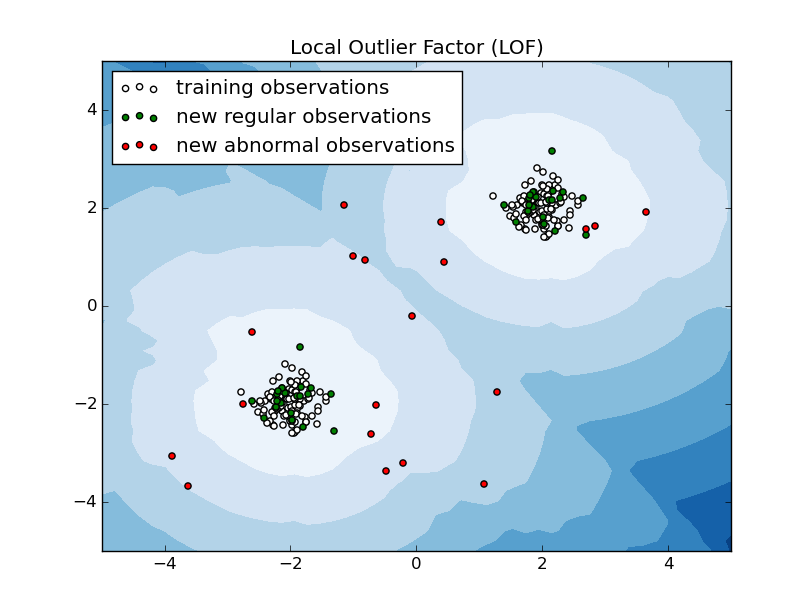
\includegraphics[width=0.9\linewidth]{fig_source/lof}
  \caption{LOF example}
  \label{fig:lof}
\end{figure}

%\begin{pythoncode} 
\begin{mdframed}[hidealllines=true, backgroundcolor=lightgray] 
\begin{minted}[fontfamily=courier, fontsize=\scriptsize]{python}
"""
=================================================
Anomaly detection with Local Outlier Factor (LOF)
=================================================

This example uses the LocalOutlierFactor estimator
for anomaly detection.
"""

import numpy as np
import matplotlib.pyplot as plt
from sklearn.neighbors import LocalOutlierFactor

np.random.seed(42)

# Generate train data
X = 0.3 * np.random.randn(100, 2)
X_train = np.r_[X + 2, X - 2]
# Generate some regular novel observations
X = 0.3 * np.random.randn(20, 2)
X_test = np.r_[X + 2, X - 2]
# Generate some abnormal novel observations
X_outliers = np.random.uniform(low=-4, high=4, size=(20, 2))

# fit the model
clf = LocalOutlierFactor()
clf.fit(X_train)
y_pred_train = clf.predict(X_train)
y_pred_test = clf.predict(X_test)
y_pred_outliers = clf.predict(X_outliers)

# plot the line, the samples, and the nearest vectors to the plane
xx, yy = np.meshgrid(np.linspace(-5, 5, 50), np.linspace(-5, 5, 50))
Z = clf.decision_function(np.c_[xx.ravel(), yy.ravel()])
Z = Z.reshape(xx.shape)

plt.title("Local Outlier Factor (LOF)")
plt.contourf(xx, yy, Z, cmap=plt.cm.Blues_r)

b1 = plt.scatter(X_train[:, 0], X_train[:, 1], c='white')
b2 = plt.scatter(X_test[:, 0], X_test[:, 1], c='green')
c = plt.scatter(X_outliers[:, 0], X_outliers[:, 1], c='red')
plt.axis('tight')
plt.xlim((-5, 5))
plt.ylim((-5, 5))
plt.legend([b1, b2, c],
           ["training observations",
            "new regular observations", "new abnormal observations"],
           loc="upper left")
plt.show()
\end{minted}
\end{mdframed}
%\end{pythoncode}


\subsection{Isolation Forest examples}
The Isolation Forest strategy is illustrated in the code example below returning Figure~\ref{fig:iforest}.


\begin{minipage}{0.52\linewidth}
\centering
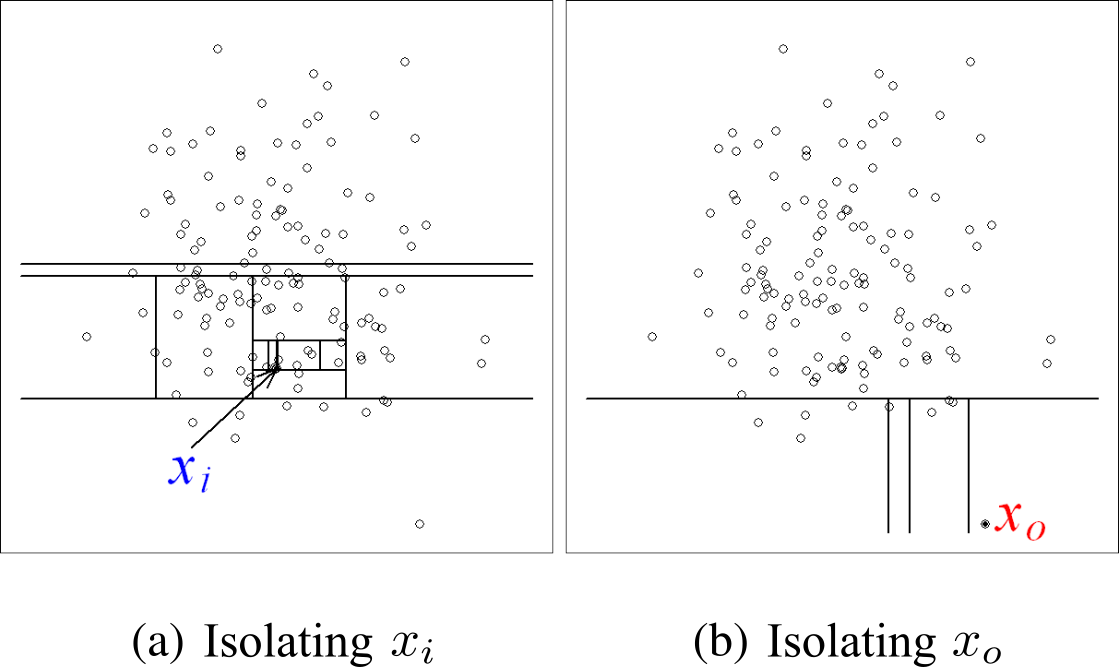
\includegraphics[scale=.95]{fig_source/ideeIF}
\captionof{figure}{Anomalies are isolated more quickly}
\label{fig:ideeIF}
\end{minipage}\hfill
\begin{minipage}{0.52\linewidth}
\centering
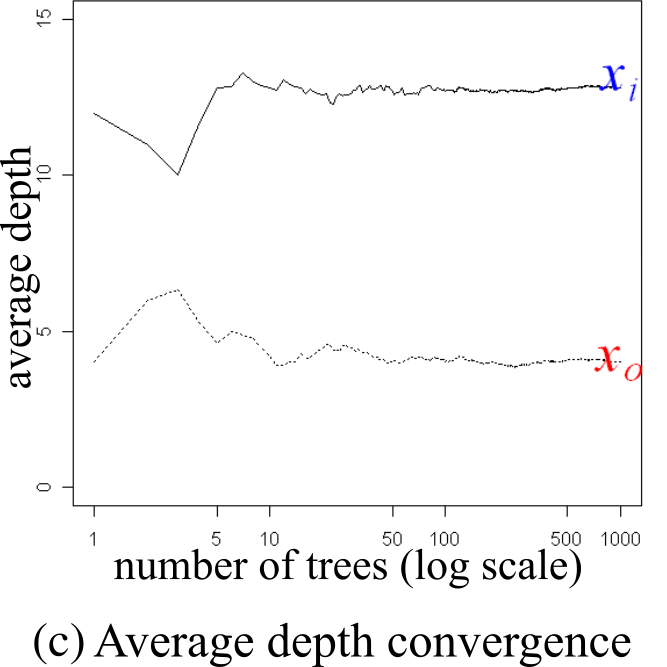
\includegraphics[scale=.95]{fig_source/convergenceIF}
\captionof{figure}{Convergence of the averaged depth}
\label{fig:convergenceIF}
\end{minipage}


\begin{figure}[!ht]
\centering
  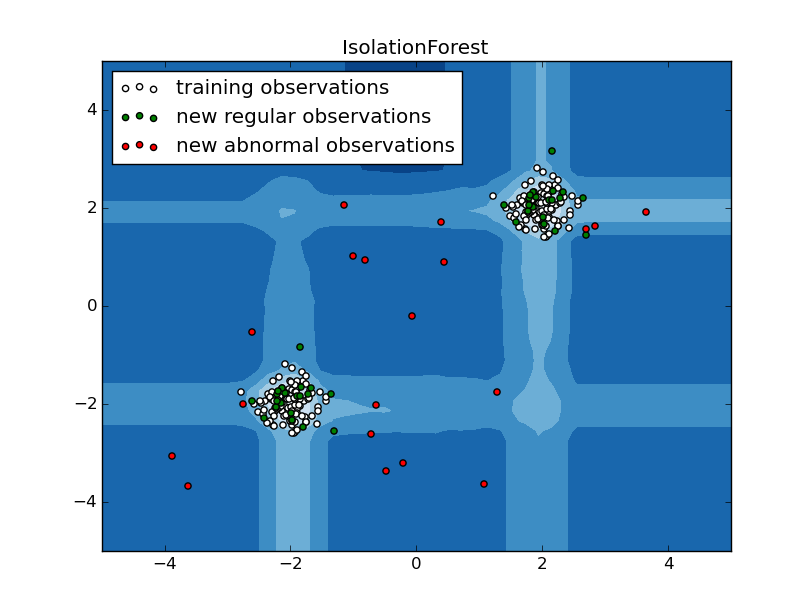
\includegraphics[width=0.8\linewidth]{fig_source/iforest}
  \caption{Isolation Forest example}
  \label{fig:iforest}
\end{figure}
~\\
%\begin{pythoncode} 
\begin{mdframed}[hidealllines=true, backgroundcolor=lightgray] 
\begin{minted}[fontfamily=courier, fontsize=\scriptsize]{python}
"""
==========================================
IsolationForest example
==========================================

An example using IsolationForest for anomaly detection.

"""

import numpy as np
import matplotlib.pyplot as plt
from sklearn.ensemble import IsolationForest

rng = np.random.RandomState(42)

# Generate train data
X = 0.3 * rng.randn(100, 2)
X_train = np.r_[X + 2, X - 2]
# Generate some regular novel observations
X = 0.3 * rng.randn(20, 2)
X_test = np.r_[X + 2, X - 2]
# Generate some abnormal novel observations
X_outliers = rng.uniform(low=-4, high=4, size=(20, 2))

# fit the model
clf = IsolationForest(max_samples=100, random_state=rng)
clf.fit(X_train)
y_pred_train = clf.predict(X_train)
y_pred_test = clf.predict(X_test)
y_pred_outliers = clf.predict(X_outliers)

# plot the line, the samples, and the nearest vectors to the plane
xx, yy = np.meshgrid(np.linspace(-5, 5, 50), np.linspace(-5, 5, 50))
Z = clf.decision_function(np.c_[xx.ravel(), yy.ravel()])
Z = Z.reshape(xx.shape)

plt.title("IsolationForest")
plt.contourf(xx, yy, Z, cmap=plt.cm.Blues_r)

b1 = plt.scatter(X_train[:, 0], X_train[:, 1], c='white')
b2 = plt.scatter(X_test[:, 0], X_test[:, 1], c='green')
c = plt.scatter(X_outliers[:, 0], X_outliers[:, 1], c='red')
plt.axis('tight')
plt.xlim((-5, 5))
plt.ylim((-5, 5))
plt.legend([b1, b2, c],
           ["training observations",
            "new regular observations", "new abnormal observations"],
           loc="upper left")
plt.show()
\end{minted}
\end{mdframed}
%\end{pythoncode}

\subsection{Comparison examples}

As a conclusion,
Figures~\ref{fig:ADcomparison1}, \ref{fig:ADcomparison2} and \ref{fig:ADcomparison3} draw a comparison of the three anomaly detection algorithms introduced in this section:

- the One-Class SVM is able to capture the shape of the
  data set, hence performing well when the data is strongly
  non-Gaussian, i.e. with two well-separated clusters;

- the Isolation Forest algorithm, is adapted to
  large-dimensional settings, even if it performs quite well in the
  examples below.

- the Local Outlier Factor measures the local deviation of a given
  data point with respect to its neighbors by comparing their local density.

The ground truth about inliers and outliers is given by the points colors
while the orange-filled area indicates which points are reported as inliers
by each method.

Here, we assume that we know the fraction of outliers in the datasets.
Thus rather than using the `predict' method of the objects, we set the
threshold on the decision function to separate out the corresponding
fraction. Anomalies are uniformly drawn according to an uniform distribution.


\begin{figure}[H]
  \centering
  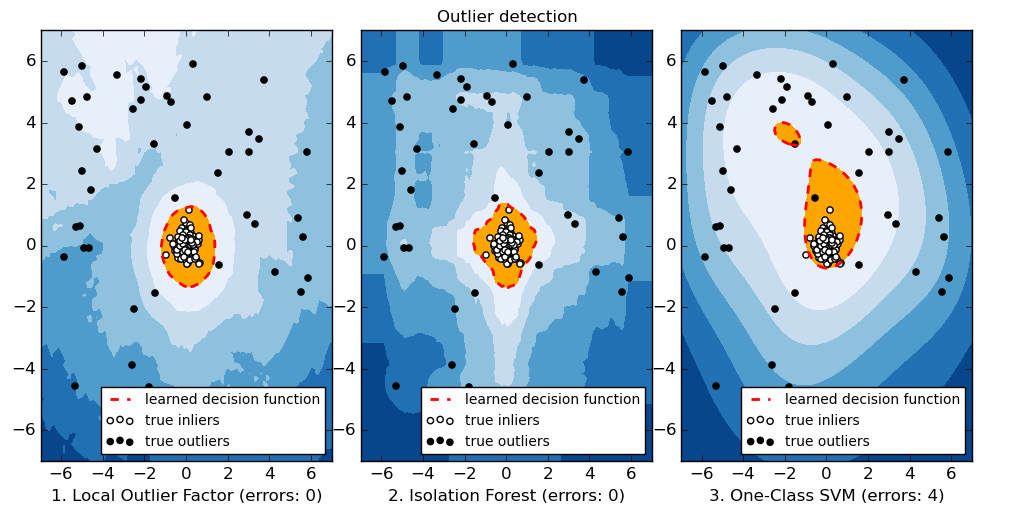
\includegraphics[width=.9\linewidth]{fig_source/ADcomparison1}
  \caption{Gaussian normal data with one single mode}
  \label{fig:ADcomparison1}
\end{figure}

\begin{figure}[H]
  \centering
  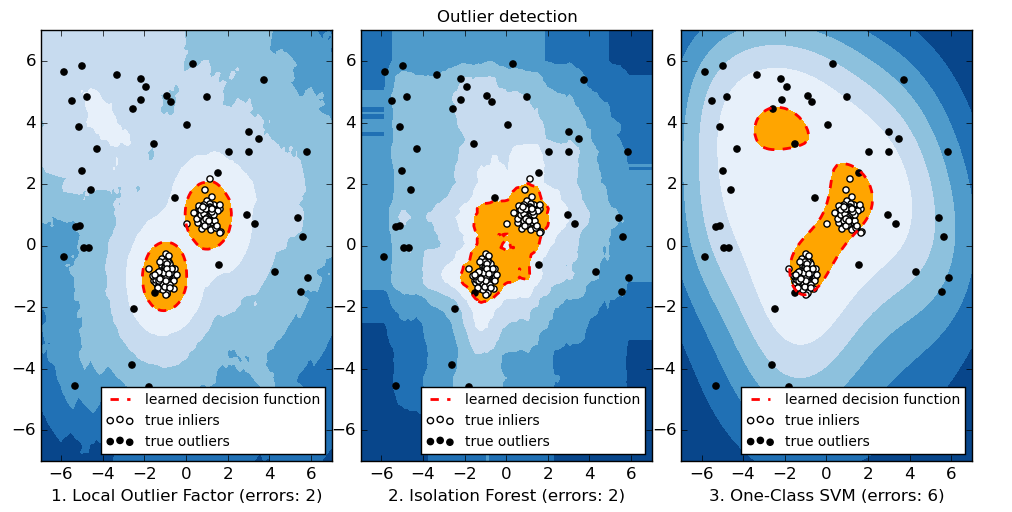
\includegraphics[width=.9\linewidth]{fig_source/ADcomparison2}
  \caption{Gaussian normal data with two modes}
  \label{fig:ADcomparison2}
\end{figure}

\begin{figure}[H]
  \centering
  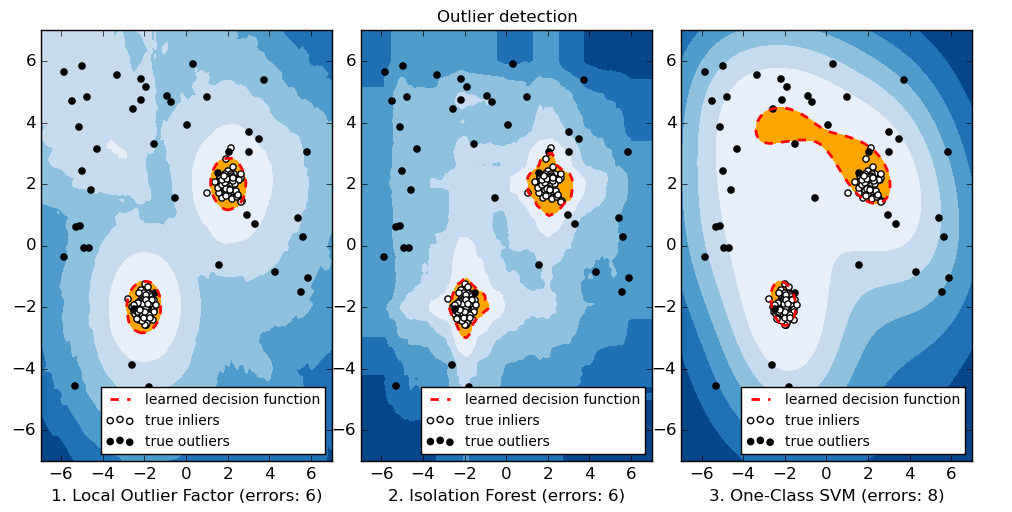
\includegraphics[width=.9\linewidth]{fig_source/ADcomparison3}
  \caption{Gaussian normal data with two strongly separate modes}
  \label{fig:ADcomparison3}
\end{figure}

% as the following code is longer than 1 page, bgcolor=lightgray option does not work: we have to use mdframed package
\begin{mdframed}[hidealllines=true, backgroundcolor=lightgray] 
\begin{minted}[fontfamily=courier, fontsize=\scriptsize]{python}
"""
==========================================
Outlier detection with several methods.
==========================================
"""

import numpy as np
import matplotlib.pyplot as plt
import matplotlib.font_manager
from scipy import stats

from sklearn import svm
from sklearn.covariance import EllipticEnvelope
from sklearn.ensemble import IsolationForest
from sklearn.neighbors import LocalOutlierFactor

rng = np.random.RandomState(42)

# Example settings
n_samples = 200
outliers_fraction = 0.25
clusters_separation = [0, 1, 2]

# define two outlier detection tools to be compared
classifiers = {
    "One-Class SVM": svm.OneClassSVM(nu=0.95 * outliers_fraction + 0.05,
                                     kernel="rbf", gamma=0.1),
    #"robust covariance estimator": EllipticEnvelope(contamination=.25),
    "Isolation Forest": IsolationForest(random_state=rng),
    "Local Outlier Factor": LocalOutlierFactor(n_neighbors=35, contamination=0.25)}

# Compare given classifiers under given settings
xx, yy = np.meshgrid(np.linspace(-7, 7, 100), np.linspace(-7, 7, 100))
n_inliers = int((1. - outliers_fraction) * n_samples)
n_outliers = int(outliers_fraction * n_samples)
ground_truth = np.ones(n_samples, dtype=int)
ground_truth[-n_outliers:] = 0

# Fit the problem with varying cluster separation
for i, offset in enumerate(clusters_separation):
    np.random.seed(42)
    # Data generation
    X1 = 0.3 * np.random.randn(n_inliers // 2, 2) - offset
    X2 = 0.3 * np.random.randn(n_inliers // 2, 2) + offset
    X = np.r_[X1, X2]
    # Add outliers
    X = np.r_[X, np.random.uniform(low=-6, high=6, size=(n_outliers, 2))]

    # Fit the model
    plt.figure(figsize=(10, 5))
    for i, (clf_name, clf) in enumerate(classifiers.items()):
        # fit the data and tag outliers
        clf.fit(X)
        y_pred = clf.decision_function(X).ravel()
        threshold = stats.scoreatpercentile(y_pred,
                                            100 * outliers_fraction)
        y_pred = y_pred > threshold
        n_errors = (y_pred != ground_truth).sum()
        # plot the levels lines and the points
        Z = clf.decision_function(np.c_[xx.ravel(), yy.ravel()])
        Z = Z.reshape(xx.shape)
        subplot = plt.subplot(1, 3, i + 1)
        subplot.contourf(xx, yy, Z, levels=np.linspace(Z.min(), threshold, 7),
                         cmap=plt.cm.Blues_r)
        a = subplot.contour(xx, yy, Z, levels=[threshold],
                            linewidths=2, colors='red')
        subplot.contourf(xx, yy, Z, levels=[threshold, Z.max()],
                         colors='orange')
        b = subplot.scatter(X[:-n_outliers, 0], X[:-n_outliers, 1], c='white')
        c = subplot.scatter(X[-n_outliers:, 0], X[-n_outliers:, 1], c='black')
        subplot.axis('tight')
        subplot.legend(
            [a.collections[0], b, c],
            ['learned decision function', 'true inliers', 'true outliers'],
            prop=matplotlib.font_manager.FontProperties(size=10),
            loc='lower right')
        subplot.set_xlabel("%d. %s (errors: %d)" % (i + 1, clf_name, n_errors))
        subplot.set_xlim((-7, 7))
        subplot.set_ylim((-7, 7))
    plt.subplots_adjust(0.04, 0.1, 0.96, 0.94, 0.1, 0.26)
    plt.suptitle("Outlier detection")

plt.show()
\end{minted}
\end{mdframed}


%\chapter{A performance criterion: the Mass-Volume Curve}

%\subsection{Elliptic Envelop}


\part{An Excess-Mass based Performance Criterion}\label{part:struct}
\chapter{On Anomaly Ranking and Excess-Mass Curves}
\label{aistat:chap}
\begin{chapabstract}
This chapter presents the details relative to the introducing section~\ref{resume:scoring}.
Learning how to rank multivariate unlabeled observations depending on their degree of abnormality/novelty is a crucial problem in a wide range of applications. In practice, it generally consists in building a real valued `scoring' function on the feature space
so as to quantify to which extent observations should be considered as abnormal.
 In the 1-d situation, measurements are generally considered as `abnormal' when they are remote from central measures such as the mean or the median. Anomaly detection then relies on tail
analysis of the variable of interest. Extensions to the multivariate setting are far from straightforward and it is precisely the main purpose of this chapter to introduce a novel and convenient (functional) criterion for measuring the performance of a scoring function regarding the anomaly ranking task, referred to as the \textit{Excess-Mass} curve ($EM$
curve). In addition, an adaptive algorithm for building a scoring function based on unlabeled data $X_1,\; \ldots,\; X_n$ with a nearly optimal $EM$-curve is proposed and is analyzed from a statistical perspective.

The material of this chapter is based on previous work published in \cite{AISTAT15}.
\end{chapabstract}



\section{Introduction}

In a great variety of applications  (\textit{e.g.} fraud detection, distributed fleet monitoring, system management in data centers), it is of crucial importance to address anomaly/novelty issues from a ranking point of view. In contrast to novelty/anomaly detection (\textit{e.g.} \cite{Kolt97, VertVert, Scholkopf2001, SHS05}), novelty/anomaly ranking is very poorly documented in the statistical learning literature (see \cite{VCTWMS} for instance). However, when confronted with
massive data, being enable to rank observations according to their supposed
degree of abnormality may significantly improve operational processes and allow for a prioritization of actions to be taken, especially in situations where human expertise required to check each observation is time-consuming.
% \par
When univariate, observations are usually considered as `abnormal'
when they are either too high or else too small compared to central
measures such as the mean or the median. In this context, anomaly/novelty analysis generally relies
on the analysis of the tail distribution of the variable of interest.  No natural (pre)~order exists on a $d$-dimensional feature space,  $\mathcal{X} \subset\mathbb{R}^d$ say, as soon as $d>1$. Extension to the multivariate setup is thus far from obvious and, in practice, the optimal ordering/ranking must be \textit{learned} from training data $X_1,\; \ldots,\; X_n$, in absence of any parametric assumptions on the underlying probability distribution describing the `normal' regime. The most straightforward manner to define a preorder on the feature space $\mathcal{X}$ is to transport the natural
order on the real half-line through a measurable \textit{scoring
  function} $s:\mathcal{X} \rightarrow \mathbb{R}_+$: the
`smaller' the score $s(X)$, the more `abnormal' the observation $X$ is
viewed. In the following, to simplify notation we assume that $\mathcal{X} = \rset^d$.
%
The whys and wherefores of scoring functions have been explained in the introduction chapter, Section~\ref{resume:scoring_function}. Estimating good scoring functions is a way to estimate level sets of the underlying density, as optimal scoring function are those whose induced level sets are exactly the ones of the density. The basic idea is that we don't need to estimate the density to obtain such level sets, but only any increasing transform of the density.
%
Any scoring function defines a preorder on $\rset^d$ and thus a ranking on a set of new observations. An important issue stated in Section~\ref{resume:scoring_function} concerns the definition of an adequate performance criterion, $\crit(s)$ say, in order to compare possible candidate scoring function and to pick one eventually: optimal scoring functions $s^*$ being then defined as those optimizing $\crit$. 
Estimating scoring function instead of the density itself precisely allows to use an other criterion than the distance to the density, which is too stringent for a level sets estimation purpose as function having exactly the same level sets as the density can be very far from the latter which such distance.

Throughout the present article, it is assumed that the distribution $F$ of the observable \rv~$X$ is absolutely continuous \wrt~Lebesgue measure $\leb$ on
$\rset^d$, with density $f(x)$.  The criterion should be thus defined in a way that the collection of level sets of an optimal scoring function $s^*(x)$ coincides with that related to $f$.  In other words, any nondecreasing transform of the density should be optimal regarding the ranking performance criterion $\crit$. According to the Empirical Risk Minimization (ERM) paradigm, a scoring function will be built in practice by optimizing an empirical version $\crit_n(s)$ of the
criterion over an adequate set of scoring functions $\S_0$ of controlled complexity (\textit{e.g.} a major class of finite {\sc VC} dimension). Hence, another desirable property to guarantee the universal consistency of ERM learning strategies is the uniform convergence of
$\crit_n(s)$ to $\crit(s)$  over such collections $\S_0$ under minimal assumptions on the distribution $F(dx)$.

As described in Section~\ref{resume:mv-curve}, a functional criterion referred to as the mass-volume curve ($MV$-curve), admissible with respect to the requirements listed above has been introduced in \cite{CLEM13}, extending somehow the concept of $\roc$ curve in the unsupervised setup. Relying on the theory of \textit{minimum volume} sets (see Section~\ref{resume:mv-set}), it has been proved that the scoring functions minimizing empirical and discretized versions of the $MV$-curve criterion are accurate when the underlying distribution has compact support and a first algorithm for building nearly optimal scoring functions, based on the estimate of a finite collection of properly chosen minimum volume sets, has been introduced and analyzed. 
However, as explained in Section~\ref{resume:mv-curve}, some important drawbacks are inherent to this mass-volume curve criterion:
\begin{itemize}
\item[\textbf{1)}] When used as an performance criterion, the lebesgue measure of possibly very complex sets has to be compute.
\item[\textbf{2)}] When used as an performance criterion, the pseudo-inverse $\alpha_s^{-1}(\alpha)$ may be hard to compute.
\item[\textbf{3)}] When used as a learning criterion (in the ERM paradigm), it produces level sets which are not necessarly nested, on which may be built inaccurate scoring function. 
\item[\textbf{4)}] When used as a learning criterion, the learning rates are rather slow (of the order $n^{-1/4}$ namely), and cannot be established in the unbounded support situation.
\end{itemize}
 % See Figure~\ref{aistat:algo-problem} and related comments for an insight into the gain resulting from the concept introduced in the present paper in contrast to the $MV$ curve minimization approach relatively to the . 
 Given these limitations, it is the major goal of this chapter to propose an alternative criterion for anomaly ranking/scoring, called the \textit{Excess-Mass} curve ($EM$ curve in short) here, based on the notion of {\it density contour clusters}  \cite{Polonik95,Hartigan1987,Muller1991}. Whereas minimum volume sets are solutions of volume minimization problems under mass constraints, the latter are solutions of mass maximization under volume constraints. Exchanging this way objective and constraint, the relevance of this performance measure is thoroughly discussed and accuracy of solutions which optimize statistical counterparts of this criterion is
investigated. More specifically, rate bounds of the order $n^{-1/2}$ are proved, even in the case of unbounded support. Additionally, in contrast to the analysis carried out in \cite{CLEM13}, the model bias issue is tackled,
insofar as the assumption that the level sets of the underlying
density $f(x)$ belongs to the class of sets used to build the scoring
function is relaxed here. 

 The rest of this chapter is organized as follows. Section~\ref{aistat:sec:notations} introduces the notion of $EM$ curve and that of optimal $EM$
curve. Estimation in the compact support case is covered by Section~\ref{aistat:sec:estim}, extension to distributions with non compact support and
control of the model bias are tackled in Section~\ref{aistat:sec:ext}. A simulation study is
performed in Section~\ref{aistat:sec:simul}. All proofs are deferred to the
last section~\ref{aistat:sec:detailed_proofs}.   


% The convergence rates obtained with the EM
% criterion are faster than the one concerning here 

%  The
% criterion we promote here is referred to as the \emph{Excess-Mass
%   Curve} (\emph{EM curve} in short),  with
% the Mass-Volume Curve introduced in \cite{CLEM13}. We will see that it
% leads to scoring functions with stronger convergence rates while
% weakening assumptions.

% Given a class $\mathcal{G}$ of borelian subsets of $X$,  a minimum
% volume set $\Omega^*_{\alpha}$ over $\mathcal{G}$, of mass at least $\alpha\in(0,1)$, is any solution of the constrained minimization problem
% \begin{align}
% \label{aistat:MV}
%  \min_{\Omega\in\mathcal{G}}\leb(\Omega) \mbox{~~subject to~~}
%  F(\Omega)\geq \alpha\,.
% \end{align}
% The value of minimum is denoted $MV_{\mathcal{G}}(\alpha)$. Abnormal observations are those which belong to %the complementary set
% $\rset^d\setminus\Omega^*_{\alpha}$, for some large value  of
% $\alpha$. 

\section{Background and related work} \label{aistat:sec:background}
As a first go, we first recall the $MV$ curve criterion approach as introduced in Section~\ref{resume:mv-curve},
% provide a brief overview
% of the scoring approach based on  the $MV$ curve criterion,
as a basis
for comparison with that promoted in the present contribution.

% Here and throughout, the indicator function of any event $\mathcal{E}$ is denoted by $\mathds{1}_{\mathcal{E}}$, the Dirac mass at any point $x$ by $\delta_x$, $A\Delta B$ the symmetric difference between two sets $A$ and $B$ and by 

Recall that $\mathcal{S}$ is the set of all scoring functions
$s: \rset^d \rightarrow \mathbb{R}_+ $ integrable \wrt~Lebesgue
measure.
Let $s\in \mathcal{S}$. As defined in \cite{CLEM13,CLEM14}, the
$MV$-curve of $s$ is the plot of the mapping $$\alpha\in (0,1)\mapsto MV_s(\alpha) = \lambda_s \circ \alpha_s^{-1}(\alpha),$$
where 
\begin{equation}
\begin{aligned}
\label{aistat:eq:alpha}
\alpha_s(t) &= \mathbb{P}(s(X) \ge t),\\ 
\lambda_s(t) &=\leb(\{x \in \rset^d, s(x) \ge t\})
  \end{aligned}
\end{equation}

 and $H^{-1}$ denotes the pseudo-inverse of any cdf $H:\mathbb{R}\rightarrow (0,1)$.
%
This induces a partial ordering on the set of all scoring functions: $s$ is
preferred to $s'$ if $MV_{s}(\alpha) \le MV_{s'}(\alpha)$ for all
$\alpha\in(0,1)$.
One may show that $MV^*(\alpha)\leq MV_s(\alpha)$ for all $\alpha\in (0,1)$ and any scoring function $s$, where $MV^*(\alpha)$ is the optimal value of the constrained minimization problem
\begin{equation}\label{aistat:eq:MV}\min_{\Gamma~ borelian} ~\leb(\Gamma) \mbox{~subject to~} \mathbb{P}(X \in \Gamma) \ge \alpha.
\end{equation}
Suppose now that $F(dx)$ has a density $f(x)$ satisfying the following assumptions:

\noindent $\mathbf{A_1}$ {\it The density $f$ is bounded, \textit{i.e.} $\vert \vert f(X)\vert\vert_{\infty}<+\infty~.$} \\
\noindent $\mathbf{A_2}$ {\it The density $f$ has no flat parts: $\forall c\geq 0$, $\mathbb{P}\{f(X)=c\}=0~.$}\\~\\
 One may then show that the curve $MV^*$ is actually a $MV$ curve, that is related to (any increasing transform of) the density $f$ namely: $MV^*=MV_f$. In addition, the  minimization problem \eqref{aistat:eq:MV} has a unique solution
$\Gamma_\alpha^*$ of mass $\alpha$ exactly, referred to as \textit{minimum volume set} (see Section~\ref{resume:mv-set}): $$MV^*(\alpha)=\leb(\Gamma^*_\alpha) ~~~\text{and}~~~ F(\Gamma_\alpha^*)=\alpha .$$ Anomaly scoring can be then viewed as the problem of building a scoring function $s(x)$ based on training data such that $MV_s$ is (nearly) minimum everywhere, \textit{i.e.} minimizing $$\|MV_{s}-MV^*\|_{\infty}:=\sup_{\alpha\in[0,1]}\vert MV_s(\alpha)-MV^*(\alpha)\vert.$$
% The minimizer $\Omega_\alpha^*$ is a \emph{minimum volume set}.%, where $\Omega_\alpha^*$.%  is
% any solution of the above minimization problem.
% and that in the case where $g$ is a nondecreasing transform of $f$, $MV_g=MV^*$.\\
% Under assumptions $\mathbf{A}_1$-$\mathbf{A}_2$, $MV^*$ is continuous on $(0,1)$ and uniformly continuous on $[0,1-\epsilon]$ for all $\epsilon \in (0,1)$ (when the support of $F(dx)$ is compact, uniform continuity holds on the whole interval $[0,1]$).
Since $F$ is unknown, a minimum volume set estimate $\widehat{\Gamma}^*_{\alpha}$ can be defined as the solution of \eqref{aistat:eq:MV} when $F$ is replaced by its empirical version
$F_n=(1/n)\sum_{i=1}^n\delta_{X_i}$, minimization is restricted to a collection $\mathcal{G}$ of borelian subsets of $\rset^d$ supposed not too complex but rich enough to include all density level sets (or reasonable approximants of the latter) and $\alpha$ is replaced by $\alpha-\phi_n$, where the {\it tolerance parameter} $\phi_n$ is a probabilistic upper bound for the supremum $\sup_{\Gamma\in \mathcal{G}}\vert F_n(\Gamma)-F(\Gamma) \vert$. Refer to \cite{Scott2006} for further details. The set $\mathcal{G}$ should ideally offer statistical and computational advantages both at the same time. Allowing for fast search on the one hand and being sufficiently complex to capture the geometry of target density level sets on the other.
%: $\inf_{\Omega \in \mathcal{G}} \leb(\Omega \Delta \Omega^*_\alpha )$ should be small for any $\alpha$, $\Delta$ denoting the symmetric difference.
In \cite{CLEM13}, a method consisting in preliminarily estimating a collection of minimum volume sets related to target masses $0<\alpha_1<\ldots<\alpha_K<1$ forming a subdivision of $(0,1)$ based on training data so as to build a scoring function $$s=\sum_k \mathds{1}_{x\in \hat \Gamma_{\alpha_k}^*}$$ has been proposed and analyzed. Under adequate assumptions (related to $\mathcal{G}$, the perimeter of the $\Gamma^*_{\alpha_k}$'s and the subdivision step in particular) and for an appropriate choice of $K=K_n$ either under the very restrictive assumption that $F(dx)$ is compactly supported or else by restricting the convergence analysis to $[0,1-\epsilon]$ for $\epsilon>0$, excluding thus the tail behavior of the distribution $F$ from the scope of the analysis, rate bounds of the order $\mathcal{O}_{\mathbb{P}}(n^{-1/4})$ have been established to guarantee the generalization ability of the method.

Figure~\ref{aistat:algo-problem} illustrates one problem inherent to the use of the $MV$ curve as a performance criterion for anomaly scoring in a `non asymptotic' context, due to the prior discretization along the mass-axis. In the $2$-d situation described by Figure~\ref{aistat:algo-problem} for instance, given the training sample and the partition of the feature space depicted, 
%choosing the subdivision $0,\; 1/2,\; 11/20,\; 1$
the $MV$ criterion leads to consider the sequence of empirical minimum volume sets $A_1,\; A_1\cup A_2,\; A_1\cup A_3,\; A_1\cup A_2\cup A_3$ and thus the scoring function $s_1(x)=\mathbb{I}\{x\in A_1  \}+ \mathbb{I}\{x\in A_1\cup A_2  \} + \mathbb{I}\{x\in A_1\cup A_3  \}$, whereas the scoring function $s_2(x)=\mathbb{I}\{x\in A_1  \}+ \mathbb{I}\{x\in A_1\cup A_3  \}$ is clearly more accurate.
%The objective is then to  depending on the data $X_1,...X_n$ such that $\|MV_{s}-MV^*\|_{\infty}$ is minimal. Practically, $ s$ will be %of type $\sum_k \mathds{1}_{x\in \hat \Omega_{\alpha_k}^*}  $ where $(\alpha_k)$ is a subdivision of $[0,1[$.\\
%The MV-curve criterion leads to two main results, depending on the finite or infinite size of $supp f$ :\\\\
%In the finite case and under assumptions $\mathbf{A_1}$ -
%$\mathbf{A_2}$ , and other assumptions on the perimeter of $\partial
%\Omega^*_\alpha$, on the class of $MV^*$ and on the boundedness of
%$MV^{*'}$, one may construct $ s$  such that with probability at least $1-\delta$ :
%\begin{align} 
%\|MV_{ s}-MV^*\|_{\infty, \alpha \in [0,1]} \le A~ \log(1/\delta) \left(\frac{1}{K^2} + \sqrt{\frac{B+log K}{n}}\right)\,,
%\end{align}
%where $K$ is the step of the subdivision $\alpha_k$ on which $s$ is built.\\
%In the infinite case, under additional assumptions  $\mathbf{A_3}$ - $\mathbf{A_4}$ (specified later in this paper)
%it is possible to construct $ s$ such that with probability at least
%$1-\delta$,  
%\begin{align}
%\|MV_{ s}-MV^*\|_{\infty, \alpha \in [0,1-\epsilon]} \le \frac{c(\epsilon,\delta)}{n^{1/4}}\,.
%\end{align}
%Unfortunately, the constant $c(\epsilon,\delta)$ tends to infinity as
%$\epsilon \rightarrow 0$ which forbids the  use of  this bound  for evaluating the quality of $s$ in the tail of the distribution.
\par In this work, a different functional criterion is proposed, obtained by exchanging objective and constraint functions in \eqref{aistat:eq:MV}, and it is shown that optimization of an empirical discretized version of this performance measure yields scoring rules with convergence rates of the order $\mathcal{O}_{\mathbb{P}}(1/\sqrt{n})$. In addition, the results can be extended to the situation where the support of the distribution $F$ is not compact.
%The subsequent optimal scoring function
%enjoys stronger convergence properties and a speed of convergence in
%$\frac{1}{\sqrt n}$. The   upper bound's dependance on $\epsilon$  is
%removed, which enables an extension to  the entire (infinite) support
%of $f$, namely on a set of possible mass $1$ instead of
%$1-\epsilon$. Finally, the bias of the new  model is controlled  by a
%simple bound, which can be made as small as desired by refining the discretization.


\section{The Excess-Mass curve}\label{aistat:sec:notations}
As introduced in Section~\ref{resume:em-curve}, the performance criterion we propose in order to evaluate anomaly scoring accuracy relies on 
the notion of \textit{excess mass} and \textit{density contour
clusters}, as introduced in the seminal contribution \cite{Polonik95}. The main idea is to consider a Lagrangian formulation of a constrained minimization problem, obtained by exchanging constraint and objective in \eqref{aistat:eq:MV}: for $t>0$,
\begin{equation}
\label{aistat:solomeg}
\max_{\Omega~ borelian}  \left\{ \mathbb{P}(X \in \Omega) - t \leb(\Omega) \right\}.
\end{equation}
We denote by $\Omega^*_t$ any solution of this problem. As shall be seen in the subsequent analysis  (see Proposition~\ref{aistat:propmono}
 below), compared to the $MV$ curve approach, this formulation offers certain computational and theoretical advantages both at the same time: when letting (a discretized version of) the Lagrangian multiplier $t$ increase from $0$ to infinity, one may easily obtain solutions of empirical counterparts of \eqref{aistat:solomeg} forming a \textit{nested} sequence of subsets of the feature space, avoiding thus deteriorating rate bounds by transforming the empirical solutions so as to force monotonicity.
 %This can be explained by the fact that a mass constraint introduces an additional discretization dimension (along the distributional mass) which is a priori independent of the volume discretization resulting from the (countable number of) empirical clusters. 
% is to solve a volume
%penalization problem instead of one constrained by the mass $\alpha$.
%Indeed, a mass constraint introduces an additional
%discretization dimension (along the distributional mass) % an other
% `discretization's dimension' along $\alpha$,
% which is a priori independent of the volume discretization  \emph{a priori} 
% resulting from the choice of a class $\mathcal{G}$. {\blue je voulais plutot dire que la discretisation en volume était nécessaire car on ne peut résoudre qu'un nombre dénombrable de problèmes d'optimisation (on est obligé d'avoir un nombre dénombrable de solutions empirique $\hat \Omega_i,i \in \mathbb{N}$)} % of  the
%  (empirical) level sets 
% for the optimization problem - which leads to a discretization in the volume of such sets, not in their mass. 
% Instead, penalizing the  volume of such sets % - namely the more one penalizes the volume, the more concentrated will be the level set -
%is deeply related  with the volume discretization and enables  better
% control of the empirical level sets (see proposition~\ref{aistat:propmono}
 %later), \emph{via} an adaptive penalization (see Section
 %\ref{aistat:sec:infiniteSupport})
%\noindent
% Analogously to the previous subsection, $X$ being a random variable on
% $\mathcal{X} \subset \mathcal{R}^d$ and $\leb$ denoting the \lebesgue
% measure on $\mathbb{R}^d$, c
%\par Consider, for any $t>0$, the  optimization problem
%
%\noindent
 %nd denote by $\Omega_t^*$ any solution. Equation~\ref{aistat:solomeg} can
%be interpreted as a  Lagrangian formulation  of \eqref{aistat:MV}, with a linear
%penality $t$ on the volume instead of the mass. 
%Define subsequently the optimal Excess
%Mass curve as :
\begin{definition}\label{aistat:def:opt}{\sc (Optimal $EM$ curve)} The optimal Excess-Mass curve related to a given probability distribution $F(dx)$ is defined as the plot of the mapping $$t>0\mapsto EM^*(t):=\max_{\Omega\text{ borelian} } \{ {\mathbb{P}} (X\in \Omega)-t\leb(\Omega) \}.$$ 
%\begin{equation*}
%EM^*(t):=  \mathbb{P}(X \in \Omega_t^*)-t.\leb(\Omega_t^*)  = \max_{\Omega~ mes.} \mathbb{P}(X \in \Omega)-t.\leb(\Omega) 
%\end{equation*}
\end{definition}
Equipped with the notation above, we have: $EM^*(t)=\mathbb{P}(X \in \Omega_t^*)-t \leb(\Omega_t^*)$ for all $t>0$.
Notice also that $EM^*(t) = 0$ for any $t>\|f\|_\infty:=\sup_{x\in \rset^d}\vert f(x)\vert$. 
% &\mbox{i.e.~~} &&\forall~ t \in [0,\|f\|_\infty],~ EM^*(t)=\max_{\Omega mes.} \mathbb{P}(X \in \Omega)-t.\leb(\Omega) \\
% &\mbox{~~and~~} &&\forall~ t ~>~ \|f\|_\infty,~ EM^*(t)=0
% The following lemma characterizes $\Omega_t^*$. % when   assumption
 % $\mathbf{A_2}$ holds true.

\begin{figure}[!ht]
\centering
\begin{tikzpicture}[scale=0.9]


\newcommand*{\maxx}{10}
\newcommand*{\maxy}{7}
\newcommand*{\maxf}{9}

%axes:
\draw[->](0,0)--(\maxx,0) node[below]{\scriptsize $t$};
\draw[->](0,0)--(0,\maxy+1) node[left]{\scriptsize $EM^*(t)$}; 

\draw[very thick](\maxf,2pt)--(\maxf,-2pt) node[below]{\scriptsize  $||f||_\infty$} ;
\draw[very thick](2pt,\maxy)--(-2pt,\maxy) node[left]{\scriptsize  1} ;
\draw[very thick](0pt,0)--(0pt,0) node[below]{\small 0} ;

\draw (\maxx/2-0.2,\maxy/2+2.3) node[below]{\scriptsize  Corresponding} ;
\draw (\maxx/2+1,\maxy/2+1.7) node[below]{\scriptsize  distributions $f$ :} ;

%petits graphs
\draw[->](2,\maxy-0.5)--(4,\maxy-0.5) node[below]{};
\draw[->](2,\maxy-0.5)--(2,\maxy+1) node[left]{}; 
\draw (2.7,\maxy-0.5) ..controls +(0,1) and +(0,-1).. (2.7,\maxy +0.5);
\draw (2.7,\maxy+0.5) ..controls +(1,0) and +(-1,0).. (3.2,\maxy +0.5);
\draw (3.2,\maxy-0.5) ..controls +(0,1) and +(0,-1).. (3.2,\maxy +0.5);
\draw (3.1,\maxy+1.2) node[below][scale=0.8]{\scriptsize  finite support} ;
%\draw (2.4,\maxy) node[thick]{1} ;

\draw[->](5,\maxy-0.5)--(7,\maxy-0.5) node[below]{};
\draw[->](5,\maxy-0.5)--(5,\maxy+1) node[left]{}; 
\draw [blue, dotted, thick] (5.7,\maxy-0.5) ..controls +(0.3,1.2) and +(-0.3,-1.2).. (6,\maxy+0.7);
\draw [blue, dotted, thick] (6,\maxy+0.7) ..controls +(0.3,-1.2) and +(-0.3,1.2).. (6.3,\maxy-0.5);
\draw (6.1,\maxy+1.2) node[below][scale=0.8]{\scriptsize finite support} ;
%\draw (5.4,\maxy) node[thick]{2} ;

\draw[->](8,\maxy-0.5)--(10,\maxy-0.5) node[below]{};
\draw[->](8,\maxy-0.5)--(8,\maxy+1) node[left]{}; 
\draw [green, dashed, thick] (8,\maxy-0.5) ..controls +(1,0.1) and +(-0.3,-0.01).. (9,\maxy+0.7);
\draw [green, dashed, thick] (9,\maxy+0.7) ..controls +(0.3,-0.01) and +(-1,0.1).. (10,\maxy-0.5);
\draw (9.3,\maxy+1.2) node[below][scale=0.8]{\scriptsize  infinite support} ;
%\draw (8.4,\maxy) node[thick]{3} ;

\draw[->](8,\maxy-3.5)--(10,\maxy-3.5) node[below]{};
\draw[->](8,\maxy-3.5)--(8,\maxy-2) node[left]{}; 
\draw [red,ultra thick] (8,\maxy-3.48) ..controls +(1,0) and +(-0.1,-0.3).. (9,\maxy-2.3);
\draw [red,ultra thick] (9,\maxy-2.3) ..controls +(0.1,-0.3) and +(-1,0).. (10,\maxy-3.48);
\draw (9,\maxy-1.8) node[below][scale=0.8]{\scriptsize  heavy tailed} ;
%\draw (8.4,\maxy-3) node[thick]{4} ;

%EM curves:
\newcommand*{\aaa}{(1/sqrt(sqrt(\maxf))+1)}
\newcommand*{\bbb}{(-1/sqrt(sqrt(\maxf)))}

\draw [red,ultra thick,domain=0:\maxf, samples=200] plot (\x,{\maxy * (\aaa/(1+sqrt(sqrt(\x)))+\bbb)} ) ;
\draw [domain=0:\maxf, samples=200] plot (\x,{\maxy * (1- 1/\maxf * \x)} ) ;

\draw [green,dashed, thick] (0,\maxy) ..controls +(0,-6) and +(-1,0).. (\maxf,0); 
\draw [blue, dotted, thick] (0,\maxy) ..controls +(3,-6) and +(-1,0).. (\maxf,0); 

%tangentes:
\tikzstyle {tangente} = [very thick, ->];
\draw [tangente,red] (0,\maxy)--++( 0,-1.5);
\draw [tangente,green,dashed] (0,\maxy)--++( 0,-1);
\draw [tangente,blue,dotted] (0,\maxy)--++( 0.5,-1);
\draw [tangente] (0,\maxy)--++( 1,-0.75);

%legende figure
%\draw (\maxx/2,-1) node[thick]{Figure 3 : Excess Mass curves} ;

\end{tikzpicture}
\caption{EM curves depending on densities}
\label{aistat:EMcurves}
\end{figure}





\begin{center}
\begin{figure}
\centering
%\resizebox{8cm}{4cm}{
\begin{tikzpicture}[scale=2.]

\draw[->](7.8,0)--(10.2,0) node[below]{\scriptsize $x$};
\draw[->](7.8,0)--(7.8,1.5) node[left]{\scriptsize $f(x)$}; 
\draw [thick] (8,0) ..controls +(1,0.1) and +(-0.3,-0.01).. (9,1.2);
\draw [thick] (9,1.2) ..controls +(0.3,-0.01) and +(-1,0.1).. (10,0);

\draw[dotted,very thick](8.60,0.3)--(8.60,0) node[right]{};
\draw[dotted,very thick](9.39,0.3)--(9.39,0) node[right]{};

%\draw (8,0.3)--(10,0.3)--(10,1.5)--(8,1.5)--(8,0.3); dessine 4 segments correspondant au 4 points

%hachurage :
\begin{scope} 
\clip (8.61,0)--(9.38,0)--(9.38,1.5)--(8.61,1.5)--(8.61,0) ; %tout ce qui est dans begin{scope} se limitera au rectangle

\path[draw,fill=lightgray] (8,0) ..controls +(1,0.1) and +(-0.3,-0.01).. (9,1.2)--
(9,1.2) ..controls +(0.3,-0.01) and +(-1,0.1).. (10,0)--
(8,0)--(10,0) --cycle;
\end{scope}

\draw[dashed](7.8,0.3)--(9.8,0.3) node[right]{\scriptsize $Q(f,\alpha)$};

%accolade :
\draw[decorate,decoration={brace}]
(9.4,-0.08)--(8.62,-0.08) node[below,pos=0.5] {\scriptsize $\Gamma_\alpha^*$};

\draw[<->]
(9.4,-0.4)--(8.62,-0.4) node[below,pos=0.5] {\scriptsize $MV^*(\alpha)$};



\draw (9,0.5) node[thick]{\scriptsize $\alpha$} ;
%\draw (8.8,-0.8) node[thick]{Figure 1: MV curve} ;

\draw[->](10.8,0)--(13.2,0) node[below]{\scriptsize $x$};
\draw[->](10.8,0)--(10.8,1.5) node[left]{\scriptsize $f(x)$}; 
\draw [thick] (11,0.01) ..controls +(1,0.1) and +(-0.3,-0.01).. (12,1.2);
\draw [thick] (12,1.2) ..controls +(0.3,-0.01) and +(-1,0.1).. (13,0.01);
\draw[dashed](10.8,0.3)--(13,0.3) node[right]{\scriptsize t};
\draw[dotted,very thick](11.60,0.3)--(11.60,0) node[right]{};
\draw[dotted,very thick](12.39,0.3)--(12.39,0) node[right]{};

%\draw (8,0.3)--(10,0.3)--(10,1.5)--(8,1.5)--(8,0.3); dessine 4 segments correspondant au 4 points

%hachurage :
\begin{scope} 
\clip (11,0.31)--(13,0.308)--(13,1.5)--(11,1.5)--(11,0.308) ; %tout ce qui est dans begin{scope} se limitera au rectangle (8,0.3)--(10,0.3)--(10,1.5)--(8,1.5)--(8,0.3)
\path[draw,fill=lightgray] (11,0) ..controls +(1,0.1) and +(-0.3,-0.01).. (12,1.2)--
(12,1.2) ..controls +(0.3,-0.01) and +(-1,0.1).. (13,0)--
(11,0.3)--(13,0.3) --cycle;
\end{scope}

%accolade :
\draw[decorate,decoration={brace}]
(12.4,-0.08)--(11.62,-0.08) node[below,pos=0.5] {\scriptsize  $\Omega_t^*$};

\draw (12,0.4) node[scale=0.85]{\scriptsize $EM^*(t)$} ;
\draw (11.8,-0.5) node[thick]{ } ;
\end{tikzpicture}
%}
\caption{Comparison between $MV^*(\alpha)$ and $EM^*(t)$}
\label{aistat:MVcurve}
\end{figure}
\end{center}



\begin{lemma}{\sc (On existence and uniqueness)}
\label{aistat:evident}
For any subset $\Omega^*_t$ solution of \eqref{aistat:solomeg}, we have
$$\{x, f(x) > t\} ~\subset~ \Omega^*_t ~\subset~ \{x, f(x) \ge t\} \text{~~~~almost-everywhere},$$
 and the sets $\{x, f(x) > t\}$ and $\{x, f(x) \ge t\}$ are both solutions of \eqref{aistat:solomeg}.
In addition, under assumption $\mathbf{A_2}$, the solution is unique:% and we have 
$$\Omega_t^*~=~ \{x, f(x) > t\}~=~ \{x, f(x) \ge t\}.$$%% \quad \text{ is unique }$$
\end{lemma}
 Observe that the curve $EM^*$ is always well-defined,
since  $ \int_{f \ge t}(f(x)-t)dx = \int_{f > t}(f(x)-t)dx$. We also point out that $EM^*(t)=\alpha(t)-t\lambda(t)$ for all $t>0$, where we set $\alpha = \alpha_f$ and
$\lambda = \lambda_f$ where $\alpha_f$ and $\lambda_f$ are defined in \eqref{aistat:eq:alpha}. % where the mappings $\alph$ and
% $\lmabda$ are we recall the notation :
% \begin{align*}
% &\alpha_s (t):= \mathbb{P}(s(X)\geq t)~~~~~~~~~~~~~~~~~~~~~~~~~~~~~~~~ \\
% &\lambda_s(t):=\leb\{x \in \rset^d,s(x)\geq t\}\\
% \mbox{and}~~~~~~~~~~~~&\\
% &\alpha (t):= \alpha_f (t) \\
% &\lambda (t):=\lambda_f(t)
% \end{align*}
% \noindent
%As for the variational properties of the EM-curve, 
%The coarea formula for Lipschitz functions leads to the result stated below.
\begin{proposition}{\sc (Derivative and convexity of $EM^*$)}  Suppose that assumptions $\mathbf{A_1}$ and $\mathbf{A_2}$ are fullfilled. Then, the mapping $EM^*$ is differentiable and we have for all $t>0$:
\label{aistat:derive}
\begin{eqnarray*}
 EM^{*'}(t)=-\lambda(t). 
\end{eqnarray*}
In addition, the mapping $t>0 \mapsto \lambda(t)$ being decreasing, the curve $EM^*$ is convex.
\end{proposition}

We now introduce the concept of Excess-Mass curve of a scoring function $s\in \S$.
%The excess mass curve (EM curve) of  such scoring functions is a
%generalization of $EM^*$.
\begin{definition} {\sc ($EM$ curves)}
The  $EM$ curve of $s\in\mathcal{S}$  \wrt~the probability
distribution $F(dx)$ of a random variable $X$ is the plot of the mapping
\begin{equation}
\label{aistat:EM}
EM_s : t \in [0, \infty[ \mapsto \sup_{A \in \{(\Omega_{s,l})_{l>0}\}} {\mathbb{P}}(X \in A) - t \leb(A),
\end{equation}
where $\Omega_{s,t}=\{ x \in \rset^d, s(x) \ge t \}$ for all $t>0$.
One may also write: $\forall t>0$, $EM_s(t)= \sup_{u>0}~ \alpha_s(u) -
t \lambda_s(u) $. Finally, under assumption $\mathbf{A_1}$, we have $EM_s(t)=0$ for every $t> \|f\|_\infty$. 
\end{definition}


%\begin{figure}%{l}{65mm}
%\centering
%\begin{tikzpicture}[scale=1.5,width=4]
%
%\draw[->](7.8,0)--(10.2,0) node[below]{x};
%\draw[->](7.8,0)--(7.8,1.5) node[left]{f(x)}; 
%\draw [thick] (8,0.01) ..controls +(1,0.1) and +(-0.3,-0.01).. (9,1.2);
%\draw [thick] (9,1.2) ..controls +(0.3,-0.01) and +(-1,0.1).. (10,0.01);
%\draw[dashed](7.8,0.3)--(10,0.3) node[right]{t};
%\draw[dotted,very thick](8.60,0.3)--(8.60,0) node[right]{};
%\draw[dotted,very thick](9.39,0.3)--(9.39,0) node[right]{};
%
%%%%%%\draw (8,0.3)--(10,0.3)--(10,1.5)--(8,1.5)--(8,0.3); dessine 4 segments correspondant au 4 points
%
%%%%%%hachurage :
%\begin{scope} 
%\clip (8,0.31)--(10,0.308)--(10,1.5)--(8,1.5)--(8,0.308) ; %tout ce qui est dans begin{scope} se limitera au rectangle (8,0.3)--(10,0.3)--(10,1.5)--(8,1.5)--(8,0.3)
%\path[draw,fill=lightgray] (8,0) ..controls +(1,0.1) and +(-0.3,-0.01).. (9,1.2)--
%(9,1.2) ..controls +(0.3,-0.01) and +(-1,0.1).. (10,0)--
%(8,0.3)--(10,0.3) --cycle;
%\end{scope}
%
%%%%%%accolade :
%\draw[decorate,decoration={brace}]
%(9.4,-0.08)--(8.62,-0.08) node[below,pos=0.5] {$\Omega_t^*$};
%
%\draw (9,0.5) node[]{\small $EM(t)$} ;
%%%%%\draw (8.8,-0.5) node[thick]{Figure 2: $EM$ curve} ;
%\end{tikzpicture}
%\caption{illustration of $EM^*$}
%\label{aistat:illustration_EM}
%\end{figure}
% 

Regarding anomaly scoring, the concept of $EM$ curve naturally induces a partial order on the set of all scoring functions: $\forall (s_1,s_2)\in \S^2$, $s_1$ is said to be more accurate than $s_2$ when $\forall t > 0, EM_{s_1}(t) \geq EM_{s_2}(t)$. Observe also that the optimal $EM$ curve introduced in Definition~\ref{aistat:def:opt} is itself the $EM$ curve of a scoring function, the $EM$ curve of any strictly increasing transform of the density $f$ namely: $EM^*=EM_f$. Hence, in the unsupervised framework, optimal scoring functions are those maximizing the $EM$ curve everywhere. In addition, maximizing $EM_s$ can be viewed as recovering a collection of subsets $(\Omega^*_t)_{t>0}$ with maximum mass when penalized by their volume in a linear fashion. An optimal scoring function is then any $s\in \S$  with the $\Omega^*_t$'s as level sets, for instance any scoring function of the form
\noindent
\begin{align}\label{aistat:score_cont}
s(x)=\int_{t=0}^{+\infty} \mathds{1}_{x\in \Omega^*_t}a(t)dt,
\end{align} 
with $a(t)>0$ (observe that $s(x)=f(x)$ for $a \equiv 1$).
% The linear  volume
%penalization can be justified by the fact that, if % is  linear in $t$ simply because if
 %$s \in L^1$,
%$t.\leb(s>t) \le \int_{s>t}s$ so that $\lambda_s(t)=\mathcal{O}(1/t)$
%when $t \rightarrow 0$. t seems then to be a natural renormalization
%of $\lambda_s(t)$.
%\begin{remark} 
%As expected, we obtain for $s$ any increasing transformation of $f$, $EM_s(t)=\mathbb{P}(X \in \Omega_t^*)-t.\leb(\Omega_t^*)=EM^*(t)$\\
%\end{remark}

\begin{proposition}
\label{aistat:propestim} ({\sc Nature of anomaly scoring}) Let $s \in \mathcal{S}$. The following properties hold true.
\begin{enumerate}
\item[(i)] The mapping $EM_s$ is non increasing on $(0,+\infty)$, takes its values in $[0,1]$ and satisfies,
%   $ \forall t\ge 0$, 
$EM_s(t) \le EM^*(t)$ for all $t\geq 0$. 
\item[(ii)]  For $t \ge 0$, we have: 
$$\inf_{u>0} \epsilon \leb (\{ s >u\}\Delta_\epsilon \{f>t\}) \le EM^*(t)-EM_s(t) \le \|f\|_\infty \inf_{u>0} \leb (\{ s >u\}\Delta\{f>t\}),$$
%
where ~$\{ s >u\}\Delta_\epsilon \{f>t\} ~:=~~ \{f>t+\epsilon\} \setminus \{ s >u\} ~~~\bigsqcup~~~ \{ s >u\} \setminus \{f>t-\epsilon\}$ should be interpreted as a symmetric difference with `an $\epsilon$ tolerance'.
\item[(iii)] Let $\epsilon >0$. Suppose that the quantity $\sup_{u>\epsilon}
  \int_{f^{-1}(\{u\})} 1/\|\nabla f(x)\|\;  d\mu(x) $ is bounded,
  where $\mu$ denotes the $(d-1)$-dimensional Hausdorff measure. Set $\epsilon_1 := \inf_{T} \|f-T\circ s\|_\infty$, where the infimum is taken over the set $\mathcal{T}$ of all borelian increasing transforms $T : \mathbb{R}_+ \rightarrow \mathbb{R}_+$. Then, 
\begin{align*}
\sup_{t\in[\epsilon + \epsilon_1,\|f\|_\infty]}|EM^*(t)-EM_s(t)| ~~\le~~  C_1 \inf_{T  \in \mathcal{T}} \|f-T\circ s\|_\infty,
\end{align*}
where $C_1=C(\epsilon_1,f)$ is a constant independent from $s(x)$.
\end{enumerate}
\end{proposition}

Assertion $(ii)$ provides a control of the pointwise difference between the
optimal $EM$ curve and $EM_s$ in terms of the error made when recovering a specific minimum volume set $\Omega_t^*$ by a level set of $s(x)$. Thus the quantity $EM^*(t)-EM_s(t)$ measures how well level sets of $s$ can approximate those of the underlying density.
Assertion $(iii)$ reveals that, if a certain increasing transform of a given scoring function $s(x)$ approximates well the density $f(x)$, then $s(x)$ is an accurate scoring function \wrt~the $EM$ criterion. %However, the reciprocal is not
%true: there are good scoring functions that are not good
%approximations of the density, \emph{e.g.}  $s=2.f$. We shall see that building a good scoring function is less complex than finding a good approximation.
As the distribution $F(dx)$ is generally unknown, $EM$ curves must be estimated. Let $s\in \S$ and $X_1,\; \ldots,\; X_n$ be an i.i.d. sample with common distribution $F(dx)$ and set $\widehat{\alpha}_s(t)=(1/n)\sum_{i=1}^n\mathds{1}_{s(X_i)\geq t}$. The empirical $EM$ curve of $s$ is then defined as $$\widehat{EM}_s(t)=\sup_{u>0}\{ \widehat{\alpha}_s(u)-t\lambda_s(u)\}~.$$ In practice, it may be difficult to estimate the volume $\lambda_s(u)$ and Monte-Carlo approximation can naturally be used for this purpose.



\section{A general approach to learn a scoring function}\label{aistat:sec:estim}

The concept of $EM$-curve provides a simple way to compare scoring functions but optimizing such a functional criterion is far from straightforward. As in \cite{CLEM13}, we propose to discretize the continuum of optimization problems and to construct a nearly optimal scoring function with level sets built by solving a finite collection of empirical versions of problem \eqref{aistat:solomeg}
over a subclass $\mathcal{G}$ of borelian subsets. In order to analyze the accuracy of this approach, we introduce the following additional assumptions.

\noindent $\mathbf{A_3}$ {\it All minimum volume sets belong to $\mathcal{G}$: $$\forall t >0,~ \Omega_t^* \in \mathcal{G}~.$$} 

\noindent $\mathbf{A_4} $ {\it The Rademacher average
 $$\mathcal{R}_n=\mathbb{E} \left[ \sup_{\Omega \in \mathcal{G}}
    \frac{1}{n} \left| \sum_{i=1}^n \epsilon_i \mathds{1}_{X_i \in
        \Omega} \right| \right]$$ is of order $\mathcal{O}_{\mathbb{P}}(n^{-1/2})$, where $(\epsilon_i)_{i \ge 1}$ is a Rademacher chaos independent of the $X_i$'s.}
        
Assumption $\mathbf{A_4}$ is very general and is fulfilled in particular when $\mathcal{G}$ is of finite VC dimension, see \cite{Kolt06}, whereas the zero bias assumption $\mathbf{A_3}$ is in contrast very restrictive. It will be relaxed in Section~\ref{aistat:sec:ext}. 
%It
%is the same as assuming that the bias $EM^*-EM_{\mathcal{G}}^*$ is
%zero, where $EM_{\mathcal{G}}^*(t)$ is the supremum of problem
%\eqref{aistat:solomeg} over the class
%$\mathcal{G}$.% It is a convenient assumption to
% start with, and will be relaxed in
% section~\ref{aistat:biais}. % $= \max_{\Omega \in \mathcal{G}}H_t(\Omega)$, which is convenient in a first time.\\

Let $\delta\in (0,1)$ and consider the complexity penalty $\Phi_n(\delta)=2 \mathcal{R}_n + \sqrt{\frac{log(1/\delta)}{2n}}$. We have for all $n \ge 1$:
\begin{equation}
\label{aistat:penality}
\mathbb{P}\left( \left\{ \sup_{G\in \mathcal{G}}\left( |P(G)- P_n(G)|-\Phi_n(\delta) \right) >0 \right\}\right) \leq \delta,
\end{equation}
see \cite{Kolt06} for instance. Denote by $F_n=(1/n)\sum_{i=1}^n \delta_{X_i}$ the empirical measure based on the training sample $X_1,\; \ldots,\; X_n$. % of the r.v $X$, which has a density $f$ with respect to the Lebesgue measure $\leb$. Let $F_n$ denote the empirical measure based on $X_1,...,X_n$, namely $F_n:=\sum_{i=1}^{n} \delta_{X_i}$, and f
For $t \ge 0$, define also the signed measures:
% \begin{align*}
% &H_t:=F-t.\leb\\
% \mbox{and~~}& H_{n,t}:=F_n-t.\leb 
% \end{align*}
\begin{align*}
&H_t(\point) =F(\point)-t \leb(\point)\\ 
\text{and ~~~~} &H_{n,t}(\point)=F_n(\point)-t \leb(\point).
\end{align*}
Equipped with these notations, for any $s \in \mathcal{S}$, we point out that one may write $EM^*(t)=\sup_{u \ge 0} H_t(\{x \in {\rset^d}, f(x) \ge u\})$ and $EM_s(t)=\sup_{u \ge 0} H_{t}(\{x \in {\rset^d}, s(x) \ge u\})$. Let $K>0$ and  $0<t_K<t_{K-1}<\ldots<t_1$. For $k$ in $\{1,\; \ldots,\; K\}$, let $\hat \Omega_{t_k}$ be an \textit{empirical $t_k$-cluster}, that is to say a borelian subset of $\rset^d$ such that
$$\hat \Omega_{t_k} \in arg\max_{\Omega \in \mathcal{G}} H_{n,t_k}(\Omega).$$
The empirical excess mass at level $t_k$ is then $H_{n,t_k}(\hat \Omega_{t_k})$. The following result reveals the benefit of viewing density level sets as solutions of \eqref{aistat:solomeg} rather than solutions of \eqref{aistat:eq:MV} (corresponding to a different parametrization of the thresholds).
%\sout{The following proposition is essential and gives full meaning to the
%definition in (\ref{aistat:EM}) of $EM_s$ and to the parameterization in $t$
%(the analogous  proposition is not true for the empirical minimum
%volume sets parameterized by  $\alpha$).}
%{ \blue The following proposition is about the behavior of empirical cluster (solution of optimization problem (\ref{aistat:solomeg})). The analogous proposition is not true in the case of the $MV$-formulation.}

\begin{proposition} 
\label{aistat:propmono}{\sc (Monotonicity)}
For any $k$ in $\{1,~\ldots,~K\}$, the subsets $\cup_{i \le k}\hat \Omega_{t_i}$ and $\cap_{i \ge k} \hat \Omega_{t_i}$ are still empirical $t_k$-clusters, just like $\hat \Omega_{t_k}$: 
\begin{align*} 
H_{n,t_k}(\cup_{i \le k}\hat \Omega_{t_i})=H_{n,t_k}(\cap_{i \ge k}\hat \Omega_{t_i})=H_{n,t_k}(\hat \Omega_{t_k}).
\end{align*}
\end{proposition}

The result above shows that monotonous (regarding the inclusion) collections of empirical clusters can always be built. Coming back to the example depicted by Figure~\ref{aistat:algo-problem}, as $t$ decreases, the $\hat \Omega_{t}$'s are successively equal to $A_1$,~ $A_1 \cup A_3$,~ and $A_1 \cup A_3 \cup A_2$, and are thus monotone as expected. This way, one fully avoids the problem inherent to the prior specification of a subdivision of the mass-axis in the $MV$-curve minimization approach (see the discussion in Section~\ref{aistat:sec:background}).

Consider an increasing sequence of empirical $t_k$ clusters $(\hat \Omega_{t_k})_{1\leq k\leq K}$ and a scoring function $s \in S$ of the form
\noindent
\begin{align}
\label{aistat:score}
s_K(x):= \sum_{k=1}^K a_k \mathds{1}_{x \in \hat{\Omega}_{t_k} }~,
\end{align}
where $a_k>0$ for every $k\in\{1,\; \ldots,\; K\}$. Notice that the scoring function \eqref{aistat:score} can be seen as a Riemann sum approximation of \eqref{aistat:score_cont} when $a_k=a(t_k)-a(t_{k+1})$. For simplicity solely, we take $a_k=t_{k}-t_{k+1}$ so that the $\hat \Omega_{t_k}$'s  are $t_k$-level sets of $s_K$, \textit{i.e} $\hat \Omega_{t_k}=\{s \ge t_k\}$ and $\{s \ge t\}= \hat \Omega_{t_k}$ if $t \in ]t_{k+1},t_{k}]$. Observe that the results established in this work remain true for other choices. In the asymptotic framework considered in the subsequent analysis, it is stipulated that $K=K_n \rightarrow \infty$ as $n\rightarrow +\infty$. We assume in addition that $\sum_{k=1}^{\infty}a_k < \infty$.
\begin{remark}
\label{aistat:orderscore}{\sc (Nested sequences)}
For $L \le K$, we have $\{\Omega_{s_L,l},l \ge 0\}=(\hat \Omega_{t_k})_{0 \le k \le L } \subset (\hat \Omega_{t_k})_{0 \le k \le K }=\{\Omega_{s_K,l},l \ge 0\}$, so that by definition, $EM_{s_L} \le EM_{s_K}$.   
\end{remark}
\begin{remark}{\sc (Related work)}
  We point out that a very similar result is proved in \cite{Polonik1998} (see Lemma 2.2 therein) concerning the
  Lebesgue measure of the symmetric differences of density clusters.
\end{remark}
\begin{remark}{\sc (Alternative construction)}
\label{aistat:mono}
It is noteworthy that, in practice, one may solve the optimization problems
$\tilde
\Omega_{t_k} \in \arg\max_{\Omega \in \mathcal{G}} H_{n,t_k}(\Omega)$
and  next form  $\hat \Omega_{t_k}= \cup_{i \le k} \tilde \Omega_{t_i}$. 
\end{remark}

The following theorem provides rate bounds describing the performance of the scoring function $s_K$ thus built with respect to the $EM$ curve criterion
 in the case where the density $f$ has compact support.
\begin{theorem}{\sc (Compact support case)}
\label{aistat:compact_support_case}
Assume that conditions $\mathbf{A_1}$, $\mathbf{A_2}$, $\mathbf{A_3}$ and $\mathbf{A_4}$ hold true, and that $f$ has a compact support. Let $\delta \in ]0,1[$, let
 $(t_k)_{k\in\{1,\;\ldots,\; K\}}$ be such that  $\sup_{1\leq k< K}(t_{k}-t_{k+1}) = \mathcal{O}(1/\sqrt{n})$.
Then, there exists a constant $A$ independent from the $t_k$'s, $n$ and
$\delta$ such that, with probability at least  $1-\delta$, we have:
\begin{align*}
\sup_{t \in ]0,t_1]} |EM^*(t)-EM_{s_K}(t)| ~~\le~~\left(A+\sqrt{2 \log(1/\delta)}~+~\leb(supp f)\right)\frac{1}{\sqrt{n}}.
\end{align*}
\end{theorem}

\begin{remark}
\label{aistat:supf}{\sc (Localization)}
The problem tackled in this work is that of scoring anomalies, which correspond to observations lying 
 outside of `large' excess mass sets, namely density clusters with parameter $t$
close to zero. It is thus essential to establish rate bounds %what is typically wanted is to bound the
for the quantity $\sup_{t \in ]0,C[} |EM^*(t)-EM_{s_K}(t)|$, where $C>0$ depends
on the proportion of the `least normal' data we want to score/rank. 
%$C$ being an estimated quantile of this proportion.
%If we aim at scoring the $25\%$ more abnormal data, $C$ will be such that $\mathbb{P}(f(X) \ge C)-C.\leb(x \in\rset^d, f(x) \ge C)$ is greater than $1/4$ (in this case, $\{x,f(x) > C\}$ contain the first quarter of the `more normal' observations).
\end{remark}

\begin{proof}[Proof of Theorem~\ref{aistat:compact_support_case} (Sketch of)]
The proof results from the following lemma, which does not use the compact support assumption on $f$ and is the starting point of the extension to the non compact support case (see Section~\ref{aistat:extension_non_compact}).
\begin{lemma} 
\label{aistat:theofini} Suppose that assumptions $\mathbf{A_1}$, $\mathbf{A_2}$, $\mathbf{A_3}$ and
  $\mathbf{A_4}$ are fulfilled. Then, for $1 \le k \le K-1$, there exists a constant $A$ independent from $n$ and  $\delta$, such that, with probability at least $1-\delta$, for $t$ in $]t_{k+1},t_{k}]$, 
\begin{align*}
|EM^*(t)-EM_{s_K}(t)| ~~\le~~\left(A+\sqrt{2log(1/\delta)}\right)\frac{1}{\sqrt n} ~+~ \lambda(t_{k+1})(t_{k}-t_{k+1}).
\end{align*}
\end{lemma}
The detailed proof of this lemma is in the Detailed Proofs Section~\ref{aistat:sec:detailed_proofs}, and is a combination on the two following results, the second one being a straightforward consequence of the derivative property of $EM^*$ (Proposition~\ref{aistat:derive}):
\begin{itemize}
\item With probability at least $1-\delta$, for $k \in \{1,...,K\}$, $$0 \le EM^*(t_{k})-EM_{s_K}(t_k) \le 2 \Phi_n(\delta)~.$$ 
\item Let $k$ in $\{1,...,K-1\}$. Then for every $t$ in $]t_{k+1},t_{k}]$,
\begin{align*}
0 \le EM^*(t)-EM^*(t_{k}) \le \lambda(t_{k+1}) (t_{k}-t_{k+1})~.
\end{align*}
\end{itemize}
\end{proof}









\section{Extensions - Further results}\label{aistat:sec:ext}
This section is devoted to extend the results of the previous one. We first relax the compact support assumption and next the one stipulating that all density level sets belong to the class $\mathcal{G}$, namely $\mathbf{A_3}$.

\subsection{Distributions with non compact support}\label{aistat:sec:infiniteSupport}
\label{aistat:extension_non_compact}
It is the purpose of this section to show that the algorithm detailed below produces a scoring function $s$ such that  $EM_s$ is uniformly close to $EM^*$ (Theorem~\ref{aistat:thmprinc}). 
 See Figure~\ref{aistat:algo-problem} as an illustration and a comparaison with the $MV$ formulation as used as a way to recover empirical minimum volume set $\hat \Gamma_\alpha$ .

\begin{algorithm} 
\caption{~~Learning a scoring function}
\label{aistat:algo1} 
Suppose that assumptions $\mathbf{A_1}$, $\mathbf{A_2}$, $\mathbf{A_3}$, $\mathbf{A_4}$ hold true.\\ Let $t_1$ such that $\max_{\Omega \in \mathcal{G}}H_{n,t_1}(\Omega)
\ge  0$. 
%\noindent
Fix  $N>0$. %  and define $t_1>t_{2}>...>t_{N}$, $\hat
% \Omega_{t_1},...,\hat \Omega_{t_N}$, such that,
For $k=1,\; \ldots,\; N$, 
\begin{enumerate} 
\item   Find  $\tilde{\Omega}_{t_k} \in \arg\max_{\Omega \in \mathcal{G}}
H_{n,t_k}(\Omega)$ , % \nonumber \\  
\item  Define $\hat \Omega_{t_k}= \cup_{i \le k} \tilde \Omega_{t_i}$
\item  Set  $ t_{k+1} =\frac{t_1}{(1+\frac{1}{\sqrt n})^{k}}   $ for $k\le N-1$. %, \nonumber 
\end{enumerate} 
% Remember that by virtue of Proposition~\ref{aistat:propmono}, $\hat
% \Omega_{t_k}$ is just as $\tilde \Omega_{t_k}$ an empirical
% $t_k$-cluster, namely $H_{n,t_k}(\hat \Omega_{t_k})=H_{n,t_k}(\tilde
% \Omega_{t_k})$.

In order to reduce the complexity, we may replace steps $1$ and $2$
with $$\hat {\Omega}_{t_k} \in \arg\max_{\Omega \supset \hat \Omega_{t_{k-1}}} H_{n,t_k}(\Omega).$$
\noindent
The resulting piecewise constant scoring function is
\begin{align}
\label{aistat:definition_sN}
s_N(x)= \sum_{k=1}^{N}(t_{k}-t_{k+1}) \mathds{1}_{x \in \hat{\Omega}_{t_k}}~.
\end{align}
% Then $s_N$ verifies with probability at least $1-\delta$:
%$\sup_{t \in ]t_N,t_1]} |EM^*(t)-EM_{s_N}(t)| \leq 2 \Phi_n(\delta) + \frac{1}{\sqrt n} = \left(A+\sqrt{2log(1/\delta)} \right)\frac{1}{\sqrt{n}}$ and $\sup_{t \in ]0,t_1]} |EM^*(t)-EM_{s_N}(t)| \leq 2 \Phi_n(\delta) + \frac{1}{\sqrt n} = \left(A+\sqrt{2log(1/\delta)} \right)\frac{1}{\sqrt{n}} + o_N(1)$
%\noindent
%where $A$ is a constant independent of $N$, $\delta$, $n$.
\end{algorithm}




\begin{center}
\begin{figure}[h!]
\centering
\begin{tikzpicture}[scale=2.5]

\draw[-](0.2,0)--(2,0) ;
\draw[-](0.2,0)--(0.2,1) ; 
\draw[-](1,0)--(1,2.2) ;
\draw[-](2,0)--(2,2.2) ;
\draw[-](0.2,1)--(2,1) ;
\draw[-](1,2.2)--(2,2.2) ;

\draw (0.8,0.5) node{\Huge .} ;
\draw (1.35,0.45) node{\Huge .} ;
\draw (1.3,0.79) node{\Huge .} ;
\draw (1.25,1.05) node{\Huge .} ;
\draw (1.31,1.57) node{\Huge .} ;
\draw (1.45,2.1) node{\Huge .} ;
\draw (1.47,1.5) node{\Huge .} ;
\draw (1.41,0.8) node{\Huge .} ;
\draw (1.49,1.2) node{\Huge .} ;
\draw (1.46,1.9) node{\Huge .} ;
\draw (1.4,1.5) node{\Huge .} ;

\draw (1.61,0.44) node{\Huge .} ;
\draw (1.68,0.71) node{\Huge .} ;
\draw (1.63,1.15) node{\Huge .} ;
\draw (1.64,1.74) node{\Huge .} ;
\draw (1.5,0.6) node{\Huge .} ;
\draw (1.7,0.15) node{\Huge .} ;
\draw (1.3,0.3) node{\Huge .} ;
\draw (1.82,0.5) node{\Huge .} ;
\draw (1.6,0.9) node{\Huge .} ;



\draw (1.5,0.2) node{$A_1$} ;
\draw (0.5,0.2) node{$A_2$} ;
\draw (1.7,2.) node{$A_3$} ;

\draw (1,-0.2) node{\scriptsize $n_1,n_2,n_3=10,9,1$} ;
\end{tikzpicture}
\caption{Unsuccessful mass-volume criterion optimization}
\parbox{13cm}{~\\ \footnotesize Sample of $n=20$ points in a $2$-d space, partitioned into three rectangles.  As $\alpha$ increases, the minimum volume sets $\hat \Gamma_{\alpha}$ are successively equal to $A_1$,~ $A_1 \cup A_2$,~ $A_1 \cup A_3$, and $A_1 \cup A_3 \cup A_2$, whereas, in the excess-mass approach, as $t$ decreases, the $\hat \Omega_{t}$'s are successively equal to $A_1$,~ $A_1 \cup A_3$,~ and $A_1 \cup A_3 \cup A_2$.
%$\hat \Omega_{10/20}=A_1$,~~ $\hat \Omega_{11/20}=A_1 \cup A_2$,~~ $\hat \Omega_{12/20}=A_1 \cup A_3$
}
\label{aistat:algo-problem}
\end{figure}
\end{center}


The main argument to extend the above results to the case where $supp f$ is not bounded is given in Lemma~\ref{aistat:theofini} in Section~\ref{aistat:sec:detailed_proofs}. The meshgrid $(t_k)$ must be chosen adaptively, in a data-driven fashion.  Let $h:~\mathbb{R}_+^* \rightarrow \mathbb{R}_+$ be a decreasing function such that $ \lim_{t \rightarrow 0}h(t)=+\infty$. Just like the previous approach, the grid is described by a decreasing sequence $(t_k)$. Let $t_1 \ge 0$, $N>0$ and define recursively $t_1>t_{2}>\ldots>t_{N}>t_{N+1}=0$, as well as $\hat \Omega_{t_1},\; \ldots,\;\hat \Omega_{t_N}$, through
\noindent
\begin{align}
\label{aistat:tk-omegak}t_{k+1}&~=~t_k -(\sqrt n)^{-1}\frac{1}{h(t_{k+1})}  \\ 
\label{aistat:tk1} \hat{\Omega}_{t_k}&~=~\arg\max_{\Omega \in \mathcal{G}} H_{n,t_k}(\Omega),
\end{align}

with the property that $\hat \Omega_{t_{k+1}} \supset \hat \Omega_{t_k}$. As pointed out in Remark~\ref{aistat:mono}, it suffices to take $\hat \Omega_{t_{k+1}}=\tilde \Omega_{t_{k+1}} \cup \hat \Omega_{t_{k}}$, where $\tilde{\Omega}_{t_{k+1}}=\arg\max_{\Omega \in \mathcal{G}} H_{n,t_k}(\Omega)$.
This yields the scoring function $s_N$ defined by (\ref{aistat:definition_sN}) such that by virtue of Lemma~\ref{aistat:theofini} (see technical details in Section~\ref{aistat:sec:detailed_proofs}), with probability at least $1-\delta$,
\begin{align*}
\sup_{t \in ]t_N,t_1]} |EM^*(t)-EM_{s_N}(t)| ~~\le~~\left(A+\sqrt{ 2 \log(1/\delta)}~+~\sup_{1\leq k\leq N}\frac{\lambda(t_k)}{h(t_k)} \right)\frac{1}{\sqrt{n}}~. 
\end{align*}
\noindent
Therefore, if we take $h$ such that $\lambda(t) = \mathcal{O}(h(t))$
as $t \rightarrow 0$, we can assume that $\lambda(t)/h(t) \le B$ for t in $]0,t_1]$ since $\lambda$ is decreasing, and we
obtain:
\begin{align}
\label{aistat:fondineq}
\sup_{t \in ]t_N,t_1]} |EM^*(t)-EM_{s_N}(t)| ~~\le~~\left(A+\sqrt{2 \log(1/\delta)} \right)\frac{1}{\sqrt{n}}~.
\end{align}
\noindent
%where $A$ is a constant independent from $N$, $\delta$ and $n$.
On the other hand from $t \leb(\{f>t\}) \le \int_{f>t} f \le 1$, we have $\lambda(t) \le 1/t$. Thus $h$ can be chosen as $h(t):=1/t$ for $t \in ]0,t_1]$. In this case, (\ref{aistat:tk1}) yields, for $k \ge 2$,
\begin{align}
\label{aistat:tk}
t_{k}=\frac{t_1}{(1+\frac{1}{\sqrt n})^{k-1}}~.
\end{align}


\begin{theorem}({\sc Unbounded support case})
\label{aistat:thmprinc}
Suppose that assumptions $\mathbf{A_1}$, $\mathbf{A_2}$, $\mathbf{A_3}$, $\mathbf{A_4}$ hold true, let $t_1>0$ and for $k \ge 2$, consider $t_k$ as defined by \eqref{aistat:tk}, $\Omega_{t_k}$ by (\ref{aistat:tk-omegak}), and $s_N$ (\ref{aistat:definition_sN}). Then there is a constant $A$ independent from $N$, $n$ and $\delta$ such that, with probability larger than $1-\delta$, we have: 
\begin{align*}
\sup_{t \in ]0,t_1]}|EM^*(t)-EM_{s_N}(t)| ~~\le~~ \left[A+\sqrt{2\log(1/\delta)}\right]\frac{1}{\sqrt n} + o_N(1),
\end{align*}
where $o_N(1)=1-EM^*(t_N)$. In addition, $s_N(x)$ converges to $s_\infty(x):=\sum_{k=1}^{\infty} (t_{k+1}-t_k)\mathds{1}_{\hat \Omega_{t_{k+1}}}$ as $N \rightarrow \infty$ and $s_\infty$ is such that, for all $\delta \in (0,1)$, we have with probability at least $1-\delta$:
\begin{align*}
\sup_{t \in ]0,t_1]}|EM^*(t)-EM_{s_\infty}(t)| \le \left[A+\sqrt{2\log(1/\delta)}\right]\frac{1}{\sqrt n}
\end{align*}
\end{theorem}
% Remember that (Remark~\ref{aistat:supf}) we don't mind if $t_1<\|f\|_\infty$, we are simply interested in bounding the quantity $\sup_{t \in ]0,C[}|EM^*(t)-EM_{s}(t)|$ with $C>0$.
% Also note that if in particular $t_1=\|f\|_\infty$, the previous inequality hold on $]t_N, \infty[$ and $]0,\infty[$ respectively, since $EM^*(t)=EM_s(t)=0$ if $t \ge \|f\|_\infty$.\\\\
% \noindent
% Consider thus the following algorithm :

\begin{proof}[Proof of Theorem~\ref{aistat:thmprinc} (Sketch of)]
The first assertion is a consequence of \eqref{aistat:fondineq} combined with the fact that
\begin{align*}
&\sup_{t \in ]0,t_N]} |EM^*(t)-EM_{s_N}(t)| ~\leq~ 1-EM_{s_N}(t_N) \\ &~~~~~~~~~~~~~~~~~~~~~~~~~~~~~~~~~~~~~~~~~~~~~~~~~~\leq~ 1-EM^*(t_N)+2\Phi_n(\delta)
\end{align*} 
holds true with probability at least $1-\delta$.
\noindent For the second part, it suffices to observe that $s_N(x)$ (absolutely) converges to $s_{\infty}$ and that, as pointed out in Remark~\ref{aistat:orderscore}, $EM_{s_N} \le EM_{s_\infty}$. 
For a detailed proof, see Section~\ref{aistat:sec:detailed_proofs}.
\end{proof}



\subsection{Bias analysis}
\label{aistat:biais}
In this subsection, we relax assumption $\mathbf{A_3}$. For any collection $\mathcal{C}$ of subsets of $\mathbb{R}^d$, $\sigma(\mathcal{C})$ denotes here the $\sigma$-algebra generated by $\mathcal{C}$.
Consider the hypothesis below.
%  This means that the previous bounds apply on $|EM_{\mathcal{G}}^*-EM_s|$ instead of $|EM^*-EM_s|$, where  $EM_{\mathcal{G}}^*(t):=\max_{\Omega \in \mathcal{G}}H_t(\Omega)$ is majored by $EM^*(t)=\max_{\Omega\; mes.}H_t(\Omega)$. Assume that : 

\noindent
$\mathbf{\tilde A_3}$  {\it There exists a countable subcollection of $\mathcal{G}$, $F=\{F_i\}_{i \ge 1}$ say, forming a partition of $\rset^d$ and such that $\sigma (F) \subset \mathcal{G}$.} 

 Denote by $f_{F}$ the best approximation (for the $L_2$-norm) of $f$ by piecewise functions on $F$, $$f_{F}(x) := \sum_{i \ge 1} \mathds{1}_{x \in F_i} \frac{1}{\leb(F_i)} \int_{F_i}f(y)dy~.$$
%For instance we can take $\mathcal{F}=\mathcal{G}=\sigma((F_i)_{i\ge 1})$ with $(F_i)_{i \ge 1}=([\frac{i_1}{l},\frac{i_1+1}{l}]\times[\frac{i_2}{l},\frac{i_2+1}{l}]\times...\times[\frac{i_d}{l},\frac{i_d+1}{l}])_{i_1,i_2,...,i_d \in \mathbb{Z}}$ the class of all sets formed by taking unions of cubes of sidelength $1/l$. Here the VC-dimension of $\mathcal{G}$ is $2$, $\mathbf{A_4}$ holds thus true.
Then, variants of Theorems~\ref{aistat:compact_support_case} and \ref{aistat:thmprinc} can be established without assumption $\mathbf{A_3}$, as soon as $\mathbf{\tilde A_3}$ holds true, at the price of the additional term $\|f-f_{F}\|_{L^1}$ in the bound, related to the inherent bias. For illustration purpose, the following result generalizes one of the inequalities stated in Theorem~\ref{aistat:thmprinc}:

\begin{theorem}({\sc Biased empirical clusters})
\label{aistat:thmprincbiais}
Suppose that assumptions $\mathbf{A_1}$, $\mathbf{A_2}$,
$\mathbf{\tilde A_3}$, $\mathbf{A_4}$ hold true, let $t_1>0$ and for $k \ge 2$ consider $t_k$ defined by (\ref{aistat:tk}), $\Omega_{t_k}$ by (\ref{aistat:tk-omegak}), and $s_N$ by (\ref{aistat:definition_sN}). Then there is a constant $A$ independent from $N$, $n$, $\delta$ such that, with probability larger than $1-\delta$, we have: 
\begin{align*}
\sup_{t \in ]0,t_1]}|EM^*(t)-EM_{s_N}(t)| ~~\le~~ \left[A+\sqrt{2\log(1/\delta)}\right]\frac{1}{\sqrt n} + \|f-f_{F}\|_{L^1}  + o_N(1), 
\end{align*}
where $o_N(1)=1-EM^*(t_N)$. 
\end{theorem}

\begin{remark}{\sc (Hypercubes)}
In practice, one defines a sequence of models $F_l\subset\mathcal{G}_l$ indexed by a tuning parameter $l$ controlling (the inverse of) model complexity, such that $\|f-f_{F_l}\|_{L^1} \rightarrow 0$ as $l \rightarrow 0$. %The parameter $p=p_n$ is generally picked so as to 
For instance, the class $F_l$ could be formed by disjoint hypercubes of side length $l$.
\end{remark}
%The previous results can thus be generalized without assumption $\mathbf{A_3}$, as soon as $\mathbf{\tilde A_3}$ holds true, and if the majoration $\|f-f_{\mathcal{F}}\|_{L^1}$ of the bias of the model is added to the previous bounds.  Note that the term $\|f-f_{\mathcal{F}}\|_{L^1}$ can be as small as desired, just choose a sufficiently fine model : for instance in the case of $(F_i)_{i \ge  1}=([\frac{i_1}{l},\frac{i_1+1}{l}]\times[\frac{i_2}{l},\frac{i_2+1}{l}]\times...\times[\frac{i_d}{l},\frac{i_d+1}{l}])_{i_1,i_2,...,i_d  \in \mathbb{Z}}$, we have $\|f-f_{\mathcal{F}}\|_{L^1} \rightarrow 0$ as $l \rightarrow \infty$.

\begin{proof}[Proof of Theorem~\ref{aistat:thmprincbiais} (Sketch of)]
The result directly follows from the following lemma, which establishes an upper bound for the bias, with the notations $EM_{\mathcal{C}}^*(t):=\max_{\Omega \in \mathcal{C}}H_t(\Omega) \le EM^*(t)=\max_{\Omega\; meas.}H_t(\Omega)$ for any class of measurable sets $\mathcal{C}$, and $\mathcal{F}:= \sigma(F)$ so that by assumption $\mathbf{A_3}$, $\mathcal{F} \subset \mathcal{G}$. Details are omitted due to space limits.\\

\begin{lemma} 
\label{aistat:propbiais}
Under assumption $\mathbf{\tilde A_3}$,  we have for every $t$ in $[0,\|f\|_\infty]$, $$0\le EM^*(t)-EM^*_{\mathcal{F}}(t) \le \|f-f_{F}\|_{L^1}~. $$ The model bias $EM^*-EM^*_{\mathcal{G}}$ is then uniformly bounded by $\|f-f_{F}\|_{L^1}$.
%where we set $$f_{F}(x) := \sum_{i \ge 1} \mathds{1}_{x \in F_i} \frac{1}{|F_i|} \int_{F_i}f(y)dy$$ the best approximation of $f$ by piecewise functions on $\mathcal{F}$.
\end{lemma}

To prove this lemma (see Section~\ref{aistat:sec:detailed_proofs} for details), one shows that:
\begin{align*}
EM^*(t)-EM^*_{\mathcal{F}}(t) \le \int_{f>t}(f-f_{F}) ~+~ \int_{\{f>t\}\setminus \{f_{F}>t\}}(f_{F}-t) ~-~\int_{\{f_{F}>t\} \setminus \{f>t\}}(f_{F}-t)~,
\end{align*}
where we use the fact that for all $t>0$, $\{ f_{F} > t \} \in \mathcal{F}$ and $\forall F~ \in~ \mathcal{F},~ \int_Gf=\int_Gf_{F}$.
It suffices then to observe that the second and the third term in the bound are non-positive.
\end{proof}


\section{Simulation examples}
\label{aistat:sec:simul}
Algorithm~\ref{aistat:algo1} is here implemented from simulated $2$-$d$ \textit{heavy-tailed} data  with common density
$f(x,y)=1/2 \times 1/(1+|x|)^3\times 1/(1+|y|)^2$. The training set is of size $n=10^5$, whereas the test set counts $10^6$ points.
For $l>0$, we set $\mathcal{G}_l=\sigma(F)$ where $F_l=\{F_i^l\}_{i\in \mathbb{Z}^2}$ and $F_i^l = [l i_1,l i_1+1]\times[l i_2,l i_2+1]$ for all $i=(i_1,i_2) \in \mathbb{Z}^2$. The bias of the model is thus bounded by $\|f-f_{F}\|_{\infty}$, vanishing as $l \rightarrow 0$ (observe that the bias is at most of order $l$ as soon as $f$ is Lipschitz for instance). The scoring function $s$ is built using the points located in $[-L,L]^2$ and setting $s=0$ outside of $[-L,L]^2$. Practically, one takes $L$ as the maximum norm value of the points in the training set, or such that an empirical estimate of $\mathbb{P}(X \in [-L,L]^2)$ is very close to $1$ (here one obtains $0.998$ for $L=500$). 
%$K^2$ is the number of hypercube in the partition of $[-L,L]^2$, such that $\frac{1}{l^2}=(\frac{K}{2.L})^2$ represents the number of hypercube partitioning a unit hypercube. 
The implementation of our algorithm involves the use of a sparse matrix to store the data in the partition of hypercubes, such that the complexity of the procedure for building the scoring function $s$ and that of the computation of its empirical $EM$-curve is very small compared to that needed to compute $f_{F_l}$ and $EM_{f_{F_l}}$, which are given here for the sole purpose of quantifying the model bias.

Figure~\ref{aistat:EMMS} illustrates as expected the deterioration of $EM_s$ for large $l$, except for $t$ close to zero: this corresponds to the model bias. However, Figure~\ref{aistat:EMMSzoom} reveals an `overfitting' phenomenon for values of $t$ close to zero, when $l$ is fairly small. 
%Figure~\ref{aistat:EMMS} and~\ref{aistat:EMMSzoom} reveal an `overfitting' phenomenon for values of $t$ close to zero, when $l$ is fairly small.
This is mainly due to the fact that subsets involved in the scoring function are then tiny in regions where there are very few observations (in the tail of the distribution). On the other hand, for the largest values of $t$, the smallest values of $l$ give the best results: the smaller the parameter $l$, the weaker the model bias and no overfitting is experienced because of the high local density of the observations.
Recalling the notation $EM_{\mathcal{G}}^*(t)=\max_{\Omega \in \mathcal{G}}H_t(\Omega) \le EM^*(t)=\max_{\Omega\; meas.}H_t(\Omega)$ so that the bias of our model is $EM^*-EM^*_{\mathcal{G}}$, Figure~\ref{aistat:EMGEM} illustrates the variations of the bias with the wealth of our model characterized by $l$ the width of the partition by hypercubes. Notice that partitions with small $l$ are not so good approximation for large $t$, but are performing as well as the other in the extreme values, namely when $t$ is close to $0$. On the top of that, those partitions have the merit not to overfit the extreme datas, which typically are isolated.
 
This empirical analysis demonstrates that introducing a notion of adaptivity for the partition $F$, with progressively growing bin-width as $t$ decays to zero and as the hypercubes are being selected in the construction of $s$ (which crucially depends on local properties of the empirical distribution), drastically improves the accuracy of the resulting scoring function in the $EM$ curve sense. 
\noindent
\begin{figure}[!ht]
\begin{minipage}[c]{.5\linewidth}
\begin{center}
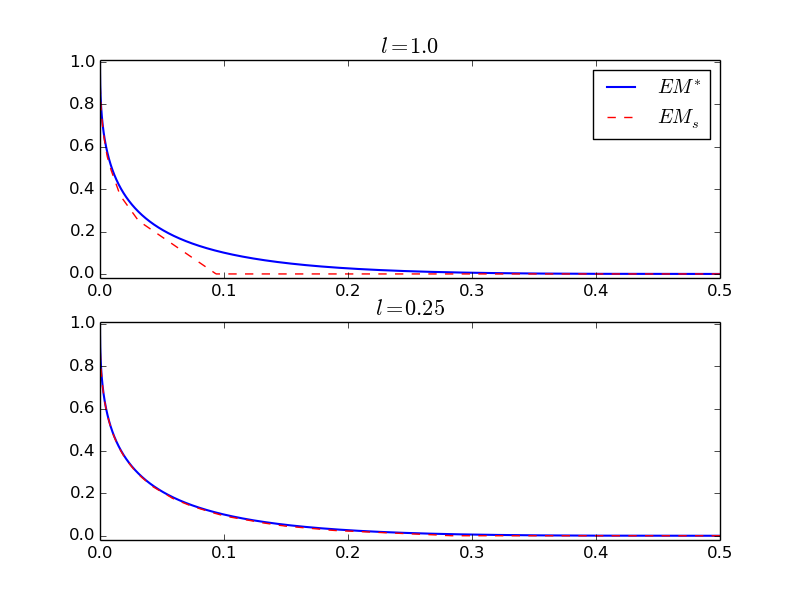
\includegraphics[width=\linewidth]{fig_source/EM-EMS.png}
\caption{Optimal and realized EM curves} %la légende
\label{aistat:EMMS}
\end{center}
\end{minipage}
\hfill
\begin{minipage}[c]{.5\linewidth}
\begin{center}
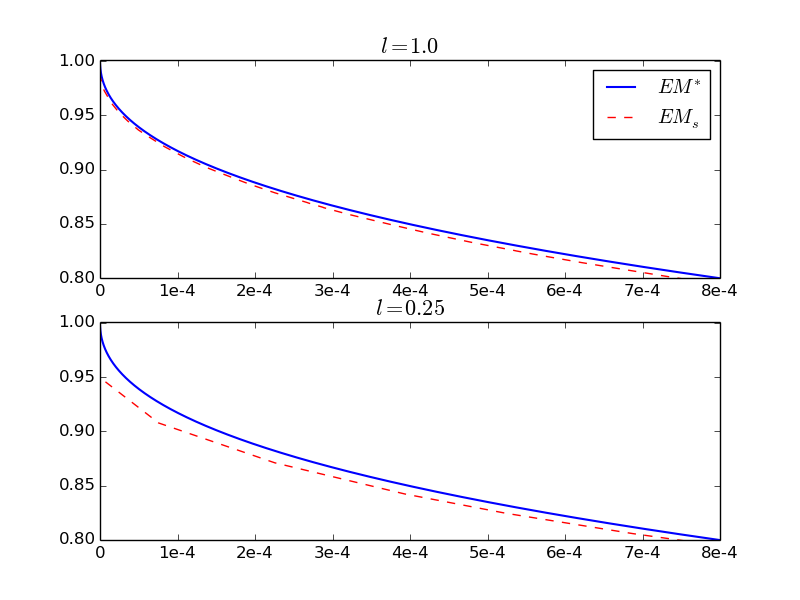
\includegraphics[width=\linewidth]{fig_source/EM-EMSzoom.png}
\caption{Zoom near 0 ~~~~~~~~~~~~~~~~~~~~~~~~~~~~~~~~~~~~~~~~~~~~~~~~~} %la légende
\label{aistat:EMMSzoom}
\end{center}
\end{minipage}
\end{figure}


\begin{figure}[!ht]
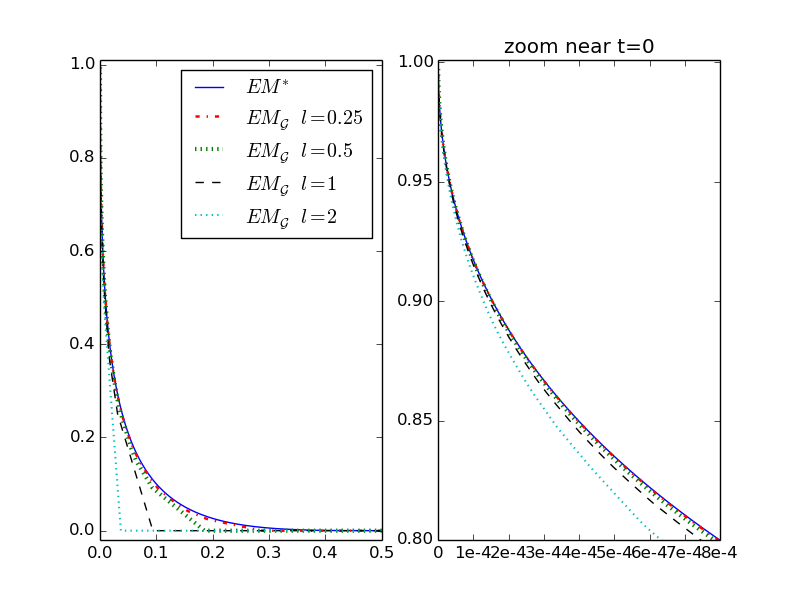
\includegraphics[width=\linewidth]{fig_source/EMG-EM.png}
\caption{$EM_\mathcal{G}$ for different $l$} %la légende
\label{aistat:EMGEM}
\end{figure}


\section{Conclusion}
Prolongating the contribution of \cite{CLEM13}, this chapter provides an alternative view (respectively, an other parameterization) of the anomaly scoring problem, leading to another adaptive method to build scoring functions, which offers theoretical and computational advantages both at the same time. This novel formulation yields a procedure producing a nested sequence of empirical density level sets, and exhibits a good performance, even in the non compact support case. 
Thus, the main drawbacks of the mass-volume curve criterion listed in the introduction section are resolved exepting drawback \textbf{1)}. In addition, the model bias has been incorporated in the rate bound analysis.
%
However, the use of the Excess-Mass criterion to measure the quality of a scoring function $s_n$ involves the computation of the Lebesgue measure  $\leb(s_n \ge u)$, just as with the Mass-Volume criterion (drawback \textbf{1)}). This is a major drawback for its use in high dimensional framework, if no prior knowledge on the form of these level sets is available.


\section{Illustrations}

Note that the scoring function we built in Algorithm~\ref{aistat:algo1} is incidentally an estimator of the density $f$ (usually called the silhouette), since $f(x)=\int_{0}^\infty \mathds{1}_{f \ge t}dt=\int_{0}^\infty \mathds{1}_{\Omega^*_t}dt$ and $s(x):= \sum_{k=1}^K (t_k-t_{k-1}) \mathds{1}_{x \in \hat{\Omega}_{t_k} }$ which is a discretization of $\int_{0}^\infty \mathds{1}_{\hat \Omega_t}dt$. This fact is illustrated in Figure~\ref{aistat:scoring3D}. Note that the silhouette does not focuse on local properties of the density, but only on its induced pre-order (level sets).
\begin{figure}[!h!]
\centering
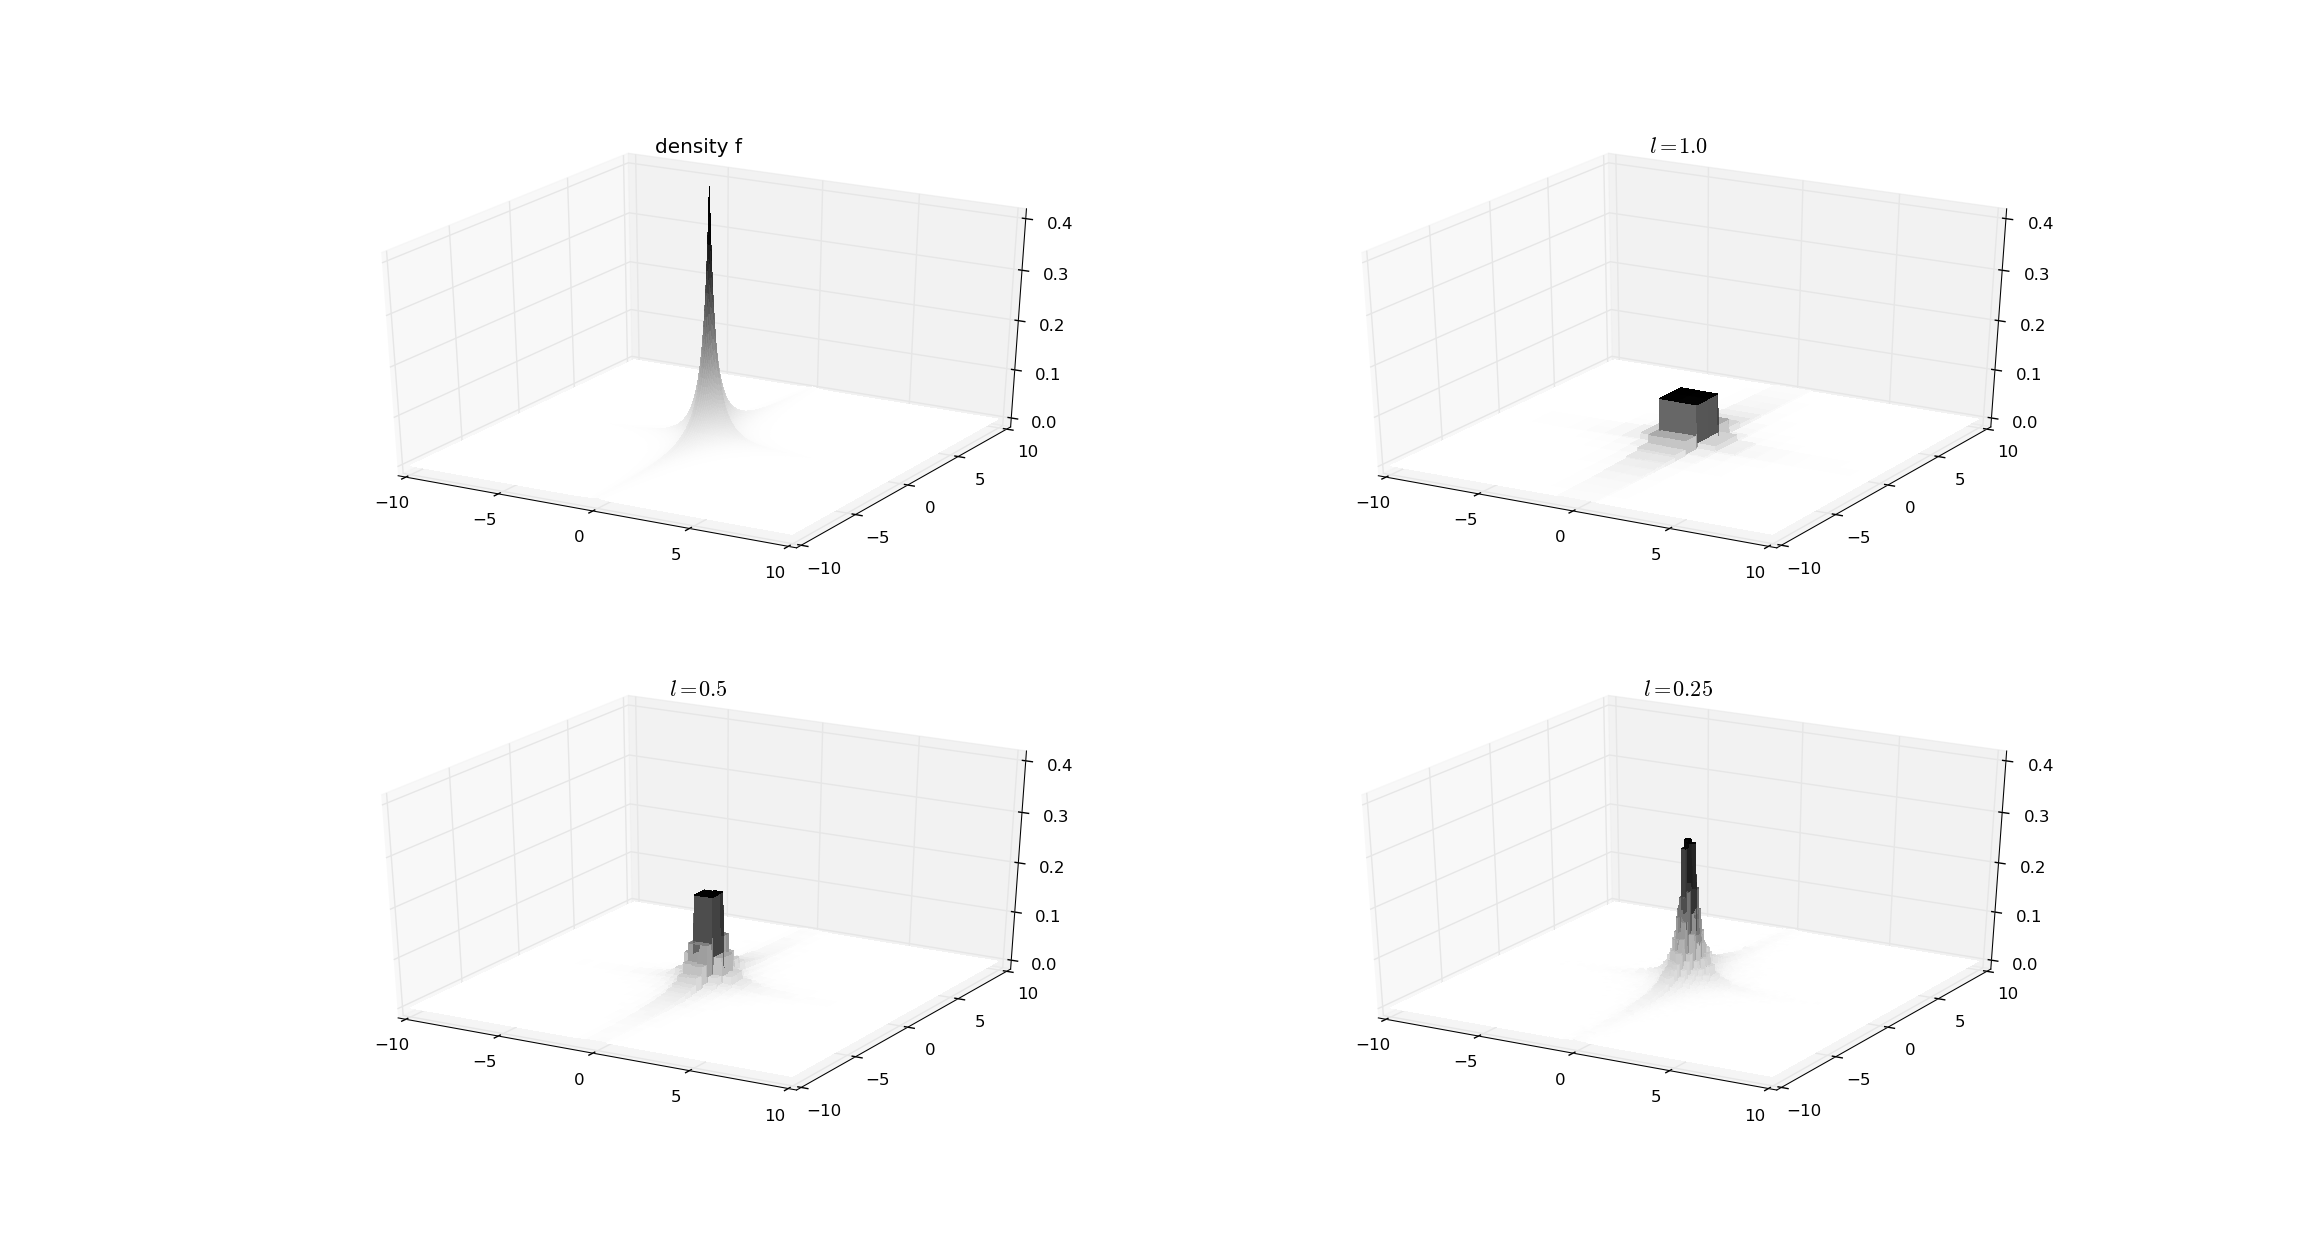
\includegraphics[width=\linewidth]{fig_source/scoring3D.png}
\caption{density and scoring functions} %la légende
\label{aistat:scoring3D}
\end{figure}






\section{Detailed Proofs}
\label{aistat:sec:detailed_proofs}
\subsection*{Proof of Proposition~\ref{aistat:derive}} Let $t>0$. Recall that $EM^{*}(t)=\alpha(t)-t \lambda(t)$ where $\alpha(t)$ denote the mass at level $t$, namely $\alpha(t)=\mathbb{P}(f(X) \ge t)$, and $\lambda(t)$ denote the volume at level $t$, i.e. $\lambda(t)=\leb(\{x, f(x) \ge t\})$. For $h>0$, let $A(h)$ denote the quantity $$A(h)=\frac{1}{h}(\alpha(t+h)-\alpha(t))$$ and $$B(h)=\frac{1}{h} (\lambda(t+h)-\lambda(t)).$$ It is straightforward to see that $A(h)$ and $B(h)$ converge when $h \rightarrow 0$, and expressing $EM^{*'}=\alpha'(t)-t\lambda'(t)-\lambda(t)$, it suffices to show that $\alpha'(t)-t\lambda'(t)=0$, namely $\lim_{h \rightarrow 0} A(h) - t~B(h) = 0$. Yet, we have $$A(h)-t~B(h)~=~\frac{1}{h} \int_{t \le f \le t+h}f-t ~\le~ \frac{1}{h} \int_{t \le f \le t+h} h  ~=~ \leb(t \le f \le t+h) \rightarrow 0$$ because $f$ has no flat part.


\subsection*{Proof of Lemma~\ref{aistat:evident}:}

On the one hand, for every $\Omega$ measurable, 
\begin{align*}
\mathbb{P}(X \in \Omega)-t~\leb(\Omega)&=\int_\Omega(f(x)-t)dx \\&\le \int_{\Omega \cap \{ f \ge t\}}(f(x)-t)dx \\&\le \int_{\{f \ge t\}}(f(x)-t)dx\\&=\mathbb{P}(f(X) \ge t)-t~\leb(\{ f \ge t\}).
\end{align*}
\noindent
It follows that $\{ f \ge t\} \in \arg\max_{A meas.}\mathbb{P}(X \in A)-t~\leb(A) $.\\

On the other hand, suppose $\Omega \in \arg\max_{A~ meas.}\mathbb{P}(X \in A)-t~\leb(A)$ and $\leb(\{f>t\} \setminus \Omega)>0$. Then there is $\epsilon > 0$ such that $\leb(\{f>t+\epsilon\} \setminus \Omega)>0$ (by sub-additivity of Leb, if it is not the case, then $ \leb(\{f>t\} \setminus \Omega) = \leb(\cup_{\epsilon \in \mathbb{Q}_+}\{ f>t+\epsilon\} \setminus \Omega)=0$ ). We have thus $$\int_{\{f>t\} \setminus \Omega} (f(x)-t)dx > \epsilon.\leb(\{f > t+ \epsilon\} \setminus \Omega) > 0~,$$ so that 
\begin{align*}
\int_{\Omega}(f(x)-t)dx &~\le~ \int_{ \{f>t\} }(f(x)-t)dx ~-~ \int_{ \{f>t \} \setminus \Omega}(f(x)-t)dx \\
&~<~ \int_{\{f>t\}}(f(x)-t)dx~,
\end{align*}

 i.e  
\begin{align*}
\mathbb{P}(X \in \Omega)-t~\leb(\Omega) ~~<~~ \mathbb{P}(f(X) \ge t) - t~\leb(\{x,f(x) \ge t\})   
\end{align*}
which is a contradiction. Thus, $\{f>t\} \subset \Omega$ Leb-almost surely.

To show that $ \Omega^*_t \subset \{x, f(x) \ge t\}$, suppose that $\leb(\Omega^*_t \cap \{f<t\}) > 0$. Then by sub-additivity of Leb just as above, there is $\epsilon >0$ such that $\leb(\Omega^*_t \cap \{f<t-\epsilon\}) > 0$ and $$\int_{\Omega^*_t \cap \{f<t-\epsilon\}} f-t \le -\epsilon.\leb(\Omega^*_t \cap \{f<t-\epsilon\})<0.$$ It follows that $$\mathbb{P}(X \in \Omega^*_t)-t~\leb(\Omega^*_t) < \mathbb{P}(X \in \Omega^*_t \setminus \{f<t-\epsilon\})-t~\leb(\Omega^*_t \setminus \{f<t-\epsilon\}),$$ which is a contradiction with the optimality of $\Omega_t^*$.



\subsection*{Proof of Proposition~\ref{aistat:propestim}}
Proving the first assertion is immediate, since $\int_{f \ge t}(f(x)-t)dx \ge \int_{s \ge t}(f(x)-t)dx$.
Let us now turn to the second assertion. We have:
\begin{align*}
EM^*(t)-EM_s(t)&=\int_{f>t}(f(x)-t)dx~-~\sup_{u>0}\int_{s>u}(f(x)-t)dx\\
&=\inf_{u>0} \int_{f>t}(f(x)-t)dx     ~-~\int_{s>u}(f(x)-t)dx~.
\end{align*}
Yet,
\begin{align*}
&\int_{\{f>t\}\setminus\{s>u\}}(f(x)-t)dx + \int_{\{s>u\}\setminus\{f>t\}}(t-f(x))dx\\
&~~~~~~~~~~~~~~~~~~~~~~~~~~~~~~~~\le (\|f\|_\infty-t).\leb\Big(\{f>t\} \setminus \{s>u\}\Big)~+~ t~\leb\Big(\{s>u\} \setminus \{f>t\}\Big),
\end{align*}
 so we obtain:
\begin{align*}
EM^*(t)-EM_s(t)  &\le~ \max(t,\|f\|_\infty-t) ~~\leb\Big(\{s>u\} \Delta \{f>t\}\Big) \\
&\le~ \|f\|_\infty .\leb\Big(\{s>u\} \Delta \{f>t\}\Big) .
\end{align*}

\noindent To prove the third point, note that:

\begin{align*}
\inf_{u>0} \leb\Big(\{s>u\} \Delta \{f>t\}\Big)~=~\inf_{T \nearrow} \leb\Big(\{Ts>t\} \Delta \{f>t\}\Big)  
\end{align*}

Yet,
\begin{align*} 
\leb\Big(\{Ts> t\} \Delta \{f>t\}\Big) &\le{\leb(\{f>t-\|Ts-f\|_\infty\} \smallsetminus \{f>t+\|Ts-f\|_\infty\})}\\
&=\lambda(t-\|Ts-f\|_\infty)~-~\lambda(t+\|Ts-f\|_\infty)\\
&=-\int_{t-\|Ts-f\|_\infty}^{t+\|Ts-f\|_\infty}\lambda'(u)du ~.
\end{align*}
\noindent
On the other hand, we have $\lambda(t)=\int_{\mathbb{R}^d}\mathds{1}_{f(x)\ge t}dx = \int_{\mathbb{R}^d} g(x) \|\nabla f(x)\|dx$, where we let $$g(x) = \frac{1}{\|\nabla f(x)\|} \mathds{1}_{\{x,\|\nabla f(x)\|>0, f(x)\ge t\}}.$$ The co-area formula (see \cite{Federer1969}, p.249, th.3.2.12) gives in this case: $$\lambda(t)=\int_{\mathbb{R}} du \int_{f^{-1}(u)}\frac{1}{\|\nabla f(x)\|} \mathds{1}_{\{x,f(x)\ge t\}}d\mu (x) = \int_{t}^\infty du \int_{f^{-1}(u)}\frac{1}{\|\nabla f(x)\|}d\mu (x)$$ so that $\lambda'(t)=-\int_{f^{-1}(u)}\frac{1}{\|\nabla f(x)\|}d\mu (x)$.\\

\noindent Let $\eta_\epsilon$ such that $ \forall u > \epsilon,~|\lambda'(u)|= \int_{f^{-1}(u)} \frac{1}{\|\nabla f(x)\|} d\mu(x)<\eta_\epsilon$.
 We obtain:
\begin{align*}
\sup_{t \in [\epsilon + \inf_{T \nearrow}\|f-Ts\|_\infty,\|f\|_\infty]} EM^*(t)-EM_s(t)~\le~ 2.\eta_\epsilon.\|f\|_\infty \inf_{T \nearrow}\|f-Ts\|_\infty.
\end{align*}
\noindent In particular, if $\inf_{T \nearrow}\|f-Ts\|_\infty \le \epsilon_1 $, 
 $$\sup_{[\epsilon + \epsilon_1,\|f\|_\infty]}|EM^*-EM_s| \le 2.\eta_{\epsilon}.\|f\|_\infty. \inf_{T \nearrow}\|f-Ts\|_\infty~. $$
\noindent


\subsection*{Proof of Proposition~\ref{aistat:propmono}}


\noindent Let $i$ in $\{1,...,K\}$. First, note  that:
\begin{align*}
H_{n,t_{i+1}}(\hat \Omega_{t_{i+1}} \cup \hat \Omega_{t_{i}}) &~=~ H_{n,t_{i+1}}(\hat \Omega_{t_{i+1}}) ~+~ H_{n,t_{i+1}}(\hat \Omega_{t_{i}} \smallsetminus \hat \Omega_{t_{i+1}}),\\
H_{n,t_{i}}(\hat \Omega_{t_{i+1}} \cap \hat \Omega_{t_{i}}) &~=~ H_{n,t_{i}}(\hat \Omega_{t_{i}}) - H_{n,t_{i}}(\hat \Omega_{t_{i}} \smallsetminus \hat \Omega_{t_{i+1}}).
\end{align*}
It follows that
\begin{align*}
&H_{n,t_{i+1}}( \hat \Omega_{t_{i+1}} \cup \hat \Omega_{t_{i}}) ~+~ H_{n,t_{i}}(\hat \Omega_{t_{i+1}} \cap \hat \Omega_{t_{i}}) \\
&~~~~~~~~~~~~~~~~~~~=~~ H_{n,t_{i+1}}(\hat \Omega_{t_{i+1}}) ~+~ H_{n,t_{i}}(\hat \Omega_{t_{i}}) ~+~ H_{n,t_{i+1}}(\hat \Omega_{t_{i}} \setminus \hat \Omega_{t_{i+1}}) ~-~ H_{n,t_{i}}(\hat \Omega_{t_{i}} \setminus \hat \Omega_{t_{i+1}})~,
\end{align*}
with $H_{n,t_{i+1}}(\hat \Omega_{t_{i}} \setminus \hat \Omega_{t_{i+1}}) - H_{n,t_{i}}(\hat \Omega_{t_{i}} \setminus \hat \Omega_{t_{i+1}}) \ge 0$ since $H_{n,t}$ is decreasing in $t$. But on the other hand, by definition of $\hat \Omega_{t_{i+1}}$ and $\hat \Omega_{t_{i}}$ we have:
\begin{align*}
H_{n,t_{i+1}}(\hat \Omega_{t_{i+1}} \cup \hat \Omega_{t_{i}}) &~~\le~~ H_{n,t_{i+1}}(\hat \Omega_{t_{i+1}})\,,\\
H_{n,t_{i}}(\hat \Omega_{t_{i+1}} \cap \hat \Omega_{t_{i}}) &~~\le~~ H_{n,t_{i}}(\hat \Omega_{t_{i}})\,.
\end{align*}
\noindent
Finally we get:
\begin{align*}
H_{n,t_{i+1}}(\hat \Omega_{t_{i+1}} \cup \hat \Omega_{t_{i}}) &~~=~~ H_{n,t_{i+1}}(\hat \Omega_{t_{i+1}})\,,\\
H_{n,t_{i}}(\hat \Omega_{t_{i+1}} \cap \hat \Omega_{t_{i}}) &~~=~~ H_{n,t_{i}}(\hat \Omega_{t_{i}})\,.
\end{align*}

\noindent
Proceeding by induction we have, for every $m$ such that $k+m \le K$:
\begin{align*}
H_{n,t_{i+m}}(\hat \Omega_{t_i} \cup \hat \Omega_{t_{i+1}} \cup ... \cup \hat \Omega_{t_{i+m}}) &~~=~~ H_{n,t_{i+m}}(\hat \Omega_{t_{i+m}})~,\\
H_{n,t_i}(\hat \Omega_{t_i} \cap \hat \Omega_{t_{i+1}} \cap ... \cap \hat \Omega_{t_{i+m}}) &~~=~~ H_{n,t_i}(\hat \Omega_{t_i})~.
\end{align*}
Taking (i=1, m=k-1) for the first equation and  (i=k, m=K-k) for the second completes the proof.\\



\subsection*{Proof of Theorem~\ref{aistat:compact_support_case}}

We shall use the following lemma:
\begin{lemma}
\label{aistat:lemmeMs}
With probability at least $1-\delta$, for $k \in \{1,...,K\}$, $$0 ~~\le~~ EM^*(t_{k})-EM_{s_K}(t_k) ~~\le~~ 2 \Phi_n(\delta).$$ 
\end{lemma}
\noindent

\textbf{Proof of Lemma~\ref{aistat:lemmeMs}: } 

Remember that by definition of $\hat \Omega_{t_k}$: $H_{n,t_k}(\hat \Omega_{t_k})=\max_{\Omega \in \mathcal{G}} H_{n,t_k}(\Omega) $ and note that:
$$EM^*(t_k)=\max_{\Omega~ meas.} H_{t_k}(\Omega)=\max_{\Omega \in \mathcal{G}} H_{t_k}(\Omega) ~~\ge~~ H_{t_k}(\hat \Omega_{t_k}). $$

%\begin{align}
%&\label{aistat:aa} \gamma(t_k)=\max_{\Omega~ meas.} \mathbb{P}(X \in \Omega) - t_k.\leb(\Omega)=\max_{\Omega~ \in \mathcal{G}} \mathbb{P}(X \in \Omega) - t_k.\leb(\Omega) \mbox{~~(by \textbf{A5})~~} \\
%&\label{aistat:bb} \gamma(t_k) ~\geq~ \beta(t_k):= \mathbb{P}(X\in \hat \Omega_{t_k})-t_k.\leb(\hat \Omega_{t_k})\\
%&\label{aistat:cc} \hat \gamma (t_k)~=~ \mathbb{P}_n(X \in \hat \Omega_{t_k})-t_k.\leb(\hat \Omega_{t_k}) ~=~ \max_{\Omega \in \mathcal{G}} ~~\mathbb{P}_n(X \in \Omega)-t_k.\leb(\Omega)
%\end{align}
On the other hand, using (\ref{aistat:penality}),  with probability at least $1-\delta$, for every $G \in \mathcal{G},~ |\mathbb{P}(G)-\mathbb{P}_n (G)| \leq \Phi_n(\delta)$. 
Hence, with probability at least $1-\delta$, for all $\Omega \in \mathcal{G}$ :
\begin{align*}
H_{n,t_k}(\Omega)-\Phi_n(\delta) ~~\le~~ H_{t_k}(\Omega) ~~\le~~ H_{n,t_k}(\Omega) + \Phi_n(\delta)
\end{align*}
\noindent so that, with probability at least $(1-\delta)$, for $k \in \{1..,K\}$,
\begin{align*}
H_{n,t_k}(\hat \Omega_{t_k})-\Phi_n(\delta) ~~\le~~ H_{t_k}(\hat \Omega_{t_k}) 
 ~~\le~~ EM^*(t_k) 
~~\le~~ H_{n,t_k}(\hat \Omega_{t_k}) + \Phi_n(\delta) ~,
\end{align*}
\noindent whereby, with probability at least $(1-\delta)$, for $k \in \{1,..,K\}$,
\begin{align*}
0 ~~\le~~ EM^*(t_k) - H_{t_k}(\hat \Omega_{t_k}) ~~\le~~ 2 \Phi_n(\delta)~.
\end{align*}


The following Lemma is a consequence of the derivative property of $EM^*$ (Proposition~\ref{aistat:derive}) 
% : the fact that $EM^{*'}=- \lambda$ (proposition~\ref{aistat:derive}) and that $\lambda$ is a decreasing function.
\begin{lemma}
\label{aistat:lemmederive}
Let $k$ in $\{1,...,K-1\}$. Then for every $t$ in $]t_{k+1},t_{k}]$,
$$0 ~~\le~~ EM^*(t)-EM^*(t_{k}) ~~\le~~ \lambda(t_{k+1}) (t_{k}-t_{k+1}).$$
\end{lemma}

\noindent Combined with Lemma~\ref{aistat:lemmeMs} and the fact that $EM_{s_K}$ is non-increasing, and writing 
\begin{align*}
EM^*(t)-EM_{s_K}(t) ~~=~~ (EM^*(t)-EM^*(t_k)) &~+~ (EM^*(t_k) ~-~ EM_{s_K}(t_k)) \\&~+~ (EM_{s_K}(t_k) ~-~ EM_{s_K}(t))
\end{align*}
this result leads to:
\begin{align*}
\forall k \in~ \{0,...,K-1\},&~ \forall t \in~ ]t_{k+1},t_{k}],
\\& ~~~~~~~~~~~~~~0 ~~\le~~ EM^*(t)-EM_{s_K}(t) ~~\le~~ 2 \Phi_n(\delta)+\lambda(t_{k+1})(t_{k}-t_{k+1}) 
\end{align*}
which gives Lemma~\ref{aistat:theofini} stated in the sketch of proof. Notice that we have not yet used the fact that $f$ has a compact support.
%and in particular, for $t \in~ ]t_{K},t_{1}]$, $|EM^*(t)-EM_{s_K}(t)| \le 2 \Phi_n(\delta)+\lambda(t_{K})\max_{k=1..K}(t_{k}-t_{k+1})$. The theorem follows directly from these arguments.

%Note in particular that with probability at least $1-\delta$, we have for all $t$ in $]t_{K},t_{1}]$:
%\begin{equation*}
%|EM^*(t)-EM_{s_K}(t)| \leq  \left(A+\sqrt{2log(1/\delta)}\right)\frac{1}{\sqrt n} + \lambda(t_{K})\sup_{1\leq k< K}(t_{k}-t_{k+1}).
%\end{equation*}

The compactness support assumption allows an extension of Lemma~\ref{aistat:lemmederive} to $k=K$, namely the inequality holds true for $t$ in $]t_{K+1},t_K]=]0,t_K]$ as soon as we let $\lambda(t_{K+1}):=\leb(supp f)$. Indeed the compactness of $supp f$ implies that $\lambda(t) \rightarrow \leb(supp f)$ as $t \rightarrow 0$. Observing that Lemma~\ref{aistat:lemmeMs} already contains the case $k=K$, this leads to, for $k$ in $\{0,...,K\}$ and $t \in~ ]t_{k+1},t_{k}],~ |EM^*(t)-EM_{s_K}(t)| \le 2 \Phi_n(\delta)+\lambda(t_{k+1})(t_{k}-t_{k+1})$. Therefore, $\lambda$ being a decreasing function bounded by $\lambda(\leb(supp f))$, we obtain the following: with probability at least $1-\delta$, we have for all $t$ in $]0,t_{1}]$,
\begin{align*}
|EM^*(t)-EM_{s_K}(t)| 
~~\le~~  \left(A+\sqrt{2log(1/\delta)}\right)\frac{1}{\sqrt n}~+~ \lambda(\leb(supp f))\sup_{1\leq k \le K}(t_{k}-t_{k+1}).
\end{align*}

%Observe that $\lambda$ is a decreasing function majored by $\leb(\supp f)$. 
%For $\epsilon > 0$, let $E_\epsilon$ denote the event \{$\sup_{t \in ]t_{K},t_{1}]} |EM^*(t)-EM_{s_K}(t)| \le (A+\sqrt{2\log(1/\delta)}+\leb(\supp f))\frac{1}{\sqrt{n}}$\}.
%We have $\mathbb{P}(E_\epsilon) \ge 1-\delta$ and the $(E_\epsilon)_\epsilon$ are decreasing sets (for inclusion) when $\epsilon$ is decreasing, so that we can make $\epsilon \rightarrow 0$ to obtain Theorem~\ref{aistat:compact_support_case}.


\subsection*{Proof of Theorem~\ref{aistat:thmprinc}}
\noindent
The first part of this theorem is a consequence of (\ref{aistat:fondineq}) combined with:
\begin{align*}
\sup_{t \in ]0,t_N]} |EM^*(t)-EM_{s_N}(t)| ~\le~ 1-EM_{s_N}(t_N) ~~\le~~ 1-EM^*(t_N)+2\Phi_n(\delta)~,
\end{align*} 
where we use the fact that $0 \le EM^*(t_N)-EM_{s_N}(t_N) \le 2 \Phi_n(\delta)$ following from Lemma~\ref{aistat:lemmeMs}.\\
\noindent To see the convergence of $s_N(x)$, note that:

\begin{align*}
s_N(x)~=~\frac{t_1}{\sqrt n} \sum_{k=1}^{\infty}\frac{1}{(1+\frac{1}{\sqrt n})^k} \mathds{1}_{x \in \hat \Omega_{t_k}} \mathds{1}_{\{k \le N\}}~~\le~~ \frac{t_1}{\sqrt n} \sum_{k=1}^{\infty} \frac{1}{(1+\frac{1}{\sqrt n})^k} ~<~ \infty,
\end{align*}

and analogically to Remark~\ref{aistat:orderscore} observe that $EM_{s_N} \le EM_{s_\infty}$ so that $\sup_{t \in ]0,t_1]} |EM^*(t)-EM_{s_\infty}(t)| \leq \sup_{t \in ]0,t_1]} |EM^*(t)-EM_{s_N}(t)|$ which prooves the last part of the theorem.

\subsection*{Proof of Lemma~\ref{aistat:propbiais}}

By definition, for every class of set $\mathcal{H}$, $EM_{\mathcal{H}}^*(t)=\max_{\Omega \in \mathcal{H}}H_t(\Omega)$.
The bias $ EM^*(t)-EM^*_{\mathcal{G}}(t)$ of the model $\mathcal{G}$ is majored by $ EM^*(t)-EM^*_{\mathcal{F}}(t)$ since $\mathcal{F} \subset \mathcal{G}$.
\noindent Remember that $$f_{F}(x) := \sum_{i \ge 1} \mathds{1}_{x \in F_i} \frac{1}{|F_i|} \int_{F_i}f(y)dy,$$ and note that for all $t>0$, $\{ f_{F} > t \} \in \mathcal{F}$. It follows that:
\begin{align*}
EM^*(t)-EM^*_{\mathcal{F}}(t) &~~=~~ \int_{f>t}(f-t)- \sup_{C \in \mathcal{F} }\int_{C}(f-t) \\
\le&~~ \int_{f>t}(f-t)- \int_{f_{F} > t}(f-t) ~~~~~~~~~~~~~~~~~\mbox{~since~} \{f_{F} > t\} ~\in~ \mathcal{F}  \\
=&~~\int_{f>t}(f-t)- \int_{f_{F} > t}(f_{F}-t) ~~~~~~~~~~~~~~~\mbox{~since~} \forall G \in \mathcal{F}, \int_Gf=\int_Gf_{F}\\
=&~~\int_{f>t}(f-t)-\int_{f>t}(f_{F}-t)+\int_{f>t}(f_{F}-t)-\int_{f_{F} > t}(f_{F}-t)\\
=&~~\int_{f>t}(f-f_{F})+\int_{\{f>t\}\setminus \{f_{F}>t\}}(f_{F}-t)-\int_{\{f_{F}>t\} \setminus \{f>t\}}(f_{F}-t)~.
\end{align*}
\noindent Observe that the second and the third term in the bound are non-positive. Therefore:
\begin{align*}
EM^*(t)-EM^*_{\mathcal{F}}(t) \le \int_{f>t}(f-f_{F}) \le \int_{\mathbb{R}^d}|f-f_{F}|~.
\end{align*}


\part{Accuracy on Extreme Regions}\label{part:vect}
\chapter{Learning the dependence structure of rare events:
a non-asymptotic study}
\label{colt}

\begin{chapabstract}
This chapter presents the details relative to the introducing section~\ref{resume:stdf}.

Assessing the probability of occurrence of extreme events is a crucial issue in various fields like finance, insurance, telecommunication or environmental sciences. In a multivariate framework, the tail dependence is characterized by the so-called \emph{stable tail dependence function} (\textsc{stdf}). Learning this structure is the keystone of multivariate extremes. Although extensive studies have proved consistency and asymptotic normality for the empirical version of the \textsc{stdf}, non-asymptotic bounds are still missing. The main purpose of this paper is to fill this gap. Taking advantage of adapted VC-type concentration inequalities, upper bounds are derived with expected rate of convergence in $O(k^{-1/2})$. The concentration tools involved in this analysis rely on a more general study of maximal deviations in low probability regions, and thus directly apply to the classification of extreme data.

The material of this chapter is based on previous work published in \cite{COLT15}.
\end{chapabstract}


\section{Introduction}
\label{colt:sec:intro}

As a first go, we briefly recall the preliminaries of Section~\ref{resume:stdf}.

To introduce the stable tail dependence function,  suppose we want to manage the risk of a
  portfolio  containing $d$ different assets,  $\mb
X = (X_1,\ldots,X_d)$.
We want to evaluate  the
probability of events of the kind 
$\{X_1 \ge x_1 \text{ or }  \dotsc \text{ or }
X_d\ge x_d \}$, for large multivariate thresholds $\mb
x=(x_1,\ldots,x_d)$.  
 
% Under not too stringent conditions on the regularity of
%   $\mb X$'s  distribution,
  \textsc{EVT} shows that under not too strong condition on the regularity of the underlying tail distribution, for large enough
  thresholds, (see Section~\ref{colt:sec:background} for details) 
\[
\P\{X_1 \ge x_1 \text{ or }  \dotsc \text{ or }
X_d\ge x_d \} \simeq 
l(p_1,\ldots,p_d), 
\]  
where $l$ is the  \emph{stable tail dependence function} and the
$p_j$'s  are the marginal exceedance probabilities, $p_j = \P(X_j\ge
x_j)$. Thus, the functional $l$  characterizes 
 the \emph{dependence} among extremes. The \emph{joint}   distribution
 (over large thresholds) 
 can thus be recovered from  the knowledge of the marginal distributions  together with
 the \textsc{stdf} $l$. In practice, $l$ can be learned % this is done   by learning the shape % of
 % % each of the  marginal tails and
 % of  the \textsc{stdf}
 from
 `moderately extreme' data, typically the $k$   `largest' ones among a
 sample of size $n$, with $k\ll n$.
 % , which is precisely
% the tail distribution function $1 - F(\mb x)$. 
% , including unobserved ones. 
Recovering the $p_j$'s can be easily done using univariate \textsc{EVT} modelling introduced in Section~\ref{back:sec:1EVT}.
However, in the multivariate case, %constrast, %However %when considering multivariate extreme events, 
there is no finite-dimensional parametrization of the dependence
structure. 
 % asymptotic tail distribution: 
The latter is characterized by % the univariate extreme value indices on the one hand, and by
% the tail dependence structure on the other hand, which is encapsulated in
the \emph{stable tail dependence function} (\textsc{stdf}) $l$.
 Estimating this functional is thus one of the main issues in multivariate \textsc{EVT}. Asymptotic properties of the empirical \textsc{stdf} have been widely studied, see \cite{Huangphd}, \cite{Drees98}, \cite{Embrechts2000} and \cite{dHF06} for the bivariate case, and \cite{Qi97}, \cite{Einmahl2012} for the general multivariate case under smoothness assumptions.

However, to the best of our knowledge, no bounds exist  %is no  established
 %  bounds 
on the finite sample error. It is precisely the purpose
of this paper to derive such non-asymptotic  bounds. Our results do
not require any assumption other than  the existence of the \textsc{stdf}.
The main idea is as follows. The empirical estimator is based on 
the empirical measure of `extreme' regions, which  are hit
 only with  low probability. It is thus enough to bound 
 maximal deviations on such low probability regions. The key consists
 in choosing an adaptive VC class, which only covers the
 latter regions, and on the other hand, to  derive  VC-type inequalities that incorporate $p$,
 the probability of hitting the class at all.%, which finally allow to . 
 

The structure of this chapter is as follows. The whys and wherefores of
 \textsc{EVT} and the \textsc{stdf} are explained in
 Section~\ref{colt:sec:background}. In Section \ref{colt:sec:concentration},
 concentration tools which rely on the general study of maximal
 deviations in low probability regions are introduced, with an
 immediate application to the framework of classification. The main result of this contribution,  a
 non-asymptotic bound on the convergence of the empirical
 \textsc{stdf}, is derived in Section \ref{colt:sec:stdf}. Section~\ref{colt:sec:conclusion} concludes.

\section{Background on the stable tail dependence function}
\label{colt:sec:background}
% A  useful setting to understand the use  of \textsc{EVT} and to give
% intuition about the \textsc{stdf} concept is that  of risk monitoring. 
% %When monitoring a risk 
% In the univariate case, it is natural to consider the $(1-p)^{th}$
% quantile of the distribution  $F$ of a random
% variable $X$,  for a given exceedance probability $p$, that is
% $x_p = \inf\{x \in \mathbb{R},~ \mathbb{P}(X > x) \le p\}$. For
% moderate values of $p$, a natural empirical estimate is  $x_{p,n} = \inf\{x \in
% \mathbb{R},~ 1/n \sum_{i=1}^n \mathds{1}_{X_i > x}\le p\}$.
% However,  if
% $p$ is very small% , say $p\le \frac{1}{n}$
% , the finite  sample $X_1,
% \ldots, X_n$  contains insufficient information and $x_{p,n}$ becomes 
% irrelevant. %  : the finite  sample $X_1, \ldots, X_n$  contains
% % insufficient information
% %  For
% % instance the is
% % useless for $p < 1/n$.  
% That is where \textsc{EVT} comes into play  by providing
% parametric estimates of large
% quantiles: % is needed in the sense it allows inference related to such extreme quantiles :
% whereas statistical inference often involves sample means and the
% central limit
% theorem, % which characterizes the limiting distribution of the sample mean,
% \textsc{EVT} handles phenomena whose behavior is % very different from those
% not ruled by an `averaging effect'. The focus is on the sample maximum
% rather than the mean.
% The primal assumption is the existence of two
% sequences $\{a_n, n \ge 1\}$ and $\{b_n, n \ge 1\}$, the $a_n$'s being
% positive, and a non-degenerate distribution function $G$ such that
% \begin{align}
% \label{colt:intro:assumption1}
% \lim_{n \to \infty} n ~\mathbb{P}\left( \frac{X - b_n}{a_n} ~\ge~ x \right) = -\log G(x)
% \end{align}
% \noindent
% % \begin{align}
% % \label{colt:intro:assumption1}
% % \lim_{n \to \infty} \mathbb{P}\left( \frac{\max_{1 \le i \le n} X_i - b_n}{a_n} ~\le~ x \right) =: G(x)
% % \end{align}
% for all continuity points $x \in \mathbb{R}$ of $G$.
% If this assumption is fulfilled -- it is the case for most  textbook
% distributions -- then $F$ is said to be in the \textit{domain of
%   attraction} of $G$, denoted $F \in DA(G)$. The tail behavior of $F$
% is then essentially characterized by $G$, which is proved to be -- up
% to  rescaling -- of the type $G(x) = \exp(-(1 + \gamma
% x)^{-1/\gamma})$ for $1 + \gamma x > 0$, $\gamma \in \mathbb{R}$,
% setting by convention $(1 + \gamma x)^{-1/\gamma} = e^{-x}$ for
% $\gamma = 0$. The sign of $\gamma$ controls the shape of the tail and
% various estimators of the rescaling sequence as well as $\gamma$ have
% been studied in great detail, see \emph{e.g.}  \cite{DEd1989},
% \cite{ELL2009}, 
% %%The Hill estimator or one of its generalizations, see
% \cite{Hill1975}, \cite{Smith1987}, \cite{BVT1996}. %, provides an
%estimate of the tail parameter $\gamma$. 
 % . The tail behavior of $F$ is then characterized by $\gamma$
% In the case $\gamma >0$ (as for the Cauchy distribution), $G$ is referred to as a Fréchet distribution and $F$ has a heavy tail. If $\gamma=0$ (as for normal distributions), $G$ is a Gumbel distribution and $F$ has a light tail. If $\gamma < 0$ (as for uniform distributions), $G$ is called a Weibull distribution and $F$ has a finite endpoint.
% Estimates of univariate extreme quantiles then rely on estimates of the parameters $a_n$, $b_n$, and $\gamma$, see \cite{DEd1989}, \cite{ELL2009}. 
%The Hill estimator or one of its generalizations, see \cite{Hill1975}, \cite{Smith1987}, \cite{BVT1996}, provides an estimate of the tail parameter $\gamma$. 

%Extensions to the multivariate setting are far from straightforward, as the tail dependence structure comes into play.
% To illustrate this point, suppose we want to assess the risk of a portfolio containing $d$ different assets $\textbf{X}=(X_1,\ldots,X_d)$. The marginal distribution of $F$ are denoted by $F_1,\ldots,F_d$.

%the asymptotics do not produce anymore a parametric model for the tail dependence structure. % as there are many possible choices of multivariate quantiles:
% If the univariate quantiles can be estimated independently, the remaining issue is then the estimation of the tail dependence structure.
% This notion of dependence is described by the STDF.

% Turning to the multivariate case, the analogue of
%  is the existence of two sequences $\{a_n, n
% \ge 1\}$ and $\{b_n, n \ge 1\}$ in $\mathbb{R}^d$, the $a_n$'s being positive,
% and a non-degenerate distribution function $G$ such that
% \begin{align}
% \label{colt:intro:assumption2}
% \lim_{n \to \infty} n ~\mathbb{P}\left( \frac{X^1 - b_n^1}{a_n^1} ~\ge~ x_1 \text{~or~} \ldots \text{~or~} \frac{X^d - b_n^d}{a_n^d} ~\ge~ x_d \right) = -\log G(\mathbf{x})
% \end{align}
% % \begin{align}
% % \label{colt:intro:assumption2}
% % \lim_{n \to \infty} \mathbb{P}\left( \frac{\max_{1 \le i \le n} X_i^1 - b_n^1}{a_n^1} ~\le~ x_1, \ldots, \frac{\max_{1 \le i \le n} X_i^d - b_n^d}{a_n^d} ~\le~ x_d \right) =: G(x)
% % \end{align}
% for all continuity points $\mathbf{x} \in \mathbb{R}^d$ of $G$. This implies
% that the margins $G_1(x_1),\ldots,G_d(x_d)$ are univariate extreme
% value distributions, namely of the type $G_j(x) = \exp(-(1 + \gamma_j
% x)^{-1/\gamma_j})$. Also, denoting by $F_1,\ldots,F_d$ the
% marginal
% distributions of $F$, assumption (\ref{colt:intro:assumption2}) implies marginal convergence, $F_i \in DA(G_i)$ for $i=1,\ldots,n$.
%  However, the tail dependence structure also comes into play
%  when considering  joint probabilities of an excess; the main issue
%  being that the asymptotics do not produce any parametric model for it.

%  To understand the structure of the limit $G$ and dispose of the
%  unknown sequences $(\mb a_n, \mb b_n)$ (which are entirely determined be the
%  marginal distributions $F_j$'s), 
%  it is convenient to
%  work with marginally standardized variables,
%  $V^j:=\frac{1}{1-F_j(X^j)}$ and $\mathbf{V}=(V^1,\ldots,V^d)$.  In
%  fact (see \cite{Resnick1987}, proposition 5.10), assumption (\ref{colt:intro:assumption2}) is
%  equivalent to marginal
%  convergences as in (\ref{colt:intro:assumption1}),  % of the marginal distributions \ie~$F_i \in DA(G_i)$, $i=1,\ldots,n$,
%  together with multivariate regular variation of $\mathbf{V}$'s
%  distribution,  which means existence of a limit measure $\mu$  on $\mb E
%  = [0,\infty]^d\setminus\{0\}$, such that % convergence of
% \begin{align}
% \label{colt:intro:regvar}
%  n~ \mathbb{P}\left( \frac{V^1 }{n} ~\ge~ v_1 \text{~or~} \cdots
%    \text{~or~} \frac{V^d }{n} ~\ge~ v_d \right) \xrightarrow[n\to\infty]{}\mu[0,\mb v]^c
% \end{align}
% \noindent (where $[0,\mathbf{v}]=[0,v_1]\times \ldots \times
% [0,v_d]$). Thus, the variable $\mb V$ satisfies
% (\ref{colt:intro:assumption2}) with $\mb a_n = (n,\ldots,n)$, $\mb b_n = (0,\ldots,0)$.
%  The so-called \emph{exponent measure} $\mu$ is finite on
% sets bounded away from $0$ and has the
% homogeneity property : $\mu(t\point) =
% t^{-1}\mu(\point)$. 
% The dependence structure of the limit $G$ in (\ref{colt:intro:assumption2})
% can be expressed in terms of $\mu$,  % then be written using the stable
% % tail dependence function ({\sc stdf}) $l$ :
% \begin{align*}
% - \log G(\mathbf{x})= \mu\left[ 0, \left(\frac{-1}{\log G_1(x_1)}, \dots ,\frac{-1}{\log G_d(x_d)}\right)\right]^c~.
% \end{align*}
% % \begin{align*}
% % G(\mathbf{x})=\exp (~ -l(-\log G_1(x_1), \dots ,-\log G_d(x_d)~ )
% % \end{align*}
% The choice of a marginal standardization  to handle $V^j$'s
% variables is somewhat arbitrary and alternative standardizations lead
% to alternative limits. %representations of the limiting dependence
% %structure. 
% Uniform margins are very helpful when it comes
% to establishing upper bounds on the deviations between empirical and mean
% measures. Define thus the standardized variable $\mathbf{U}$ %and $\mathbf{V}$
%  by $U^j =1-F_j(X^j)$. Then, it is easy to see that (\ref{colt:intro:regvar})
% % will e very  
% % The latter
% is equivalent to the
% existence of a 
% measure $\Lambda$ on $[0,\infty]^d\setminus\{+\infty\}$, such that
% % function $l : \mathbb{R}^d_+ \to \mathbb{R}_+$  such that
% % \begin{align}
% % \label{colt:stdf1}
% % \lim_{t \to 0} t^{-1} \mathbb{P} \left[ 1-F_1(X^1) \le t\, x_1
% %   ~\text{or}~ \ldots ~\text{or}~ 1-F_d(X^d) \le t\,x_d  \right] =
% % \lambda[\mb x, \infty]^c :=l(\mb x)~.
% % \end{align}
% \begin{align}
% \label{colt:stdf1}
% % \lim_{t \to 0} t^{-1} \mathbb{P} \left[ U^1 \le t\, x_1
% %   ~\text{or}~ \ldots ~\text{or}~ U^d \le t\,x_d  \right] =
% % \lambda[\mb x, \infty]^c :=l(\mb x)~. \qquad(x_j\in[0,\infty], \mb x\neq\infty)
% \lim_{t \to 0} t^{-1} \mathbb{P} \left[
%  U^1 \le t\, x_1
%    ~\text{or}~ \ldots ~\text{or}~ U^d \le t\,x_d  \right]
%  % \bigcup_{j=1}^d U^j \le t\, x_j \right] =
%  = \Lambda[\mb x, \infty]^c :=l(\mb x)~. \qquad(x_j\in[0,\infty], \mb x\neq\infty)
% \end{align}


% The limit measure $\Lambda$ is again called \emph{exponent measure}
% and the functional $l$ is known as the \emph{stable tail dependence
%   function}. 
% In a nutshell,  there
% is a one-to-one correspondence between the \textsc{stdf}  $l$  % the so-called \emph{exponent
% % measures}
%  and the measures $\mu$ and $\Lambda$, % the STDF $l$ and the angular measure
% % $\Phi$, any one of them can be used to characterize  the 
% % % The measures $\mu$ and $\Lambda$ are called exponent measures, any one
% % % of $\mu,\Lambda,l$ can be used to describe the 
% % asymptotic tail dependence of the distribution $F$ (as
% % soon as the  margins $F_j$ are known), since 
% % after each marginal had been standardized in $\mathbf{U}$ or $\mathbf{V}$.
% \begin{align}
% \label{colt:intro:1to1}
%   l(\mathbf{x}) = \mu \big( [0,\mathbf{x}^{-1}]^c \big) = \Lambda
%   \big( [\mathbf{x},\infty]^c \big)~,  %=  \int_{S^{d-1}} \max_j{w_j x_j} \phi(dw),
% \end{align}
% Further, the   \textsc{stdf}  $l$ and $\Lambda$ enjoy homogeneity properties derived from
% $\mu$, namely 
% \[l(t\mb x) = \mu[0,t^{-1}\mb x^{-1}]^c = t\mu[0,\mb x^{-1}] = tl(\mb
% x).\]

% The dependence structure of  $G$ %in (\ref{colt:intro:assumption2})
% may thus be  expressed in terms of $l$,  % then be written using the stable
% % tail dependence function ({\sc stdf}) $l$ :
% \begin{align*}
% G(\mathbf{x})=\exp (~ -l(-\log G_1(x_1), \dots ,-\log G_d(x_d)~ )
% \end{align*}

In the multivariate case, it is mathematically very convenient to decompose the joint
distribution of $\mb X = (X^1,\ldots, X^d)$  % of excesses above high thresholds 
into the margins on the
one hand, and the dependence structure on the other hand. In
particular, handling uniform margins is very helpful when it comes
to establishing upper bounds on the deviations between empirical and mean
 measures. Define thus  standardized variables $U^j = 1 - F_j(X^j)$,
 where $F_j$ is the marginal distribution function of $X^j$, and
 $\mathbf{U} = (U^1,\dotsc,U^d)$. Knowledge of the $F_j$'s and of the
 joint distribution of $\mb U$ allows to recover that of $\mb X$, %  by a
 % classical rank tranformation.% ,
 since  $\P(X_1\le x_1,\ldots, X_d\le x_d) = \P(U^1 \ge
 1 -  F_1(x_1),\ldots,U^d\ge 1-F_d(x_d))$.  % if the $F_j$'s are  continuous,
 % strictly increasing. % ,
  With these notations,  under the fairly general assumption, namely, standard multivariate regular variation of standardized variables (\ref{back:intro:regvar}), equivalent to \eqref{back:reg_var_U}, there exists a limit measure
$\Lambda$ on $[0,\infty]^d \setminus\{\infty\}$ (called the
\emph{exponent measure}) such that 
\begin{align}
\label{colt:stdf1}
% \lim_{t \to 0} t^{-1} \mathbb{P} \left[ U^1 \le t\, x_1
%   ~\text{or}~ \ldots ~\text{or}~ U^d \le t\,x_d  \right] =
% \lambda[\mb x, \infty]^c :=l(\mb x)~. \qquad(x_j\in[0,\infty], \mb x\neq\infty)
\lim_{t \to 0} t^{-1} \mathbb{P} \left[
 U^1 \le t\, x_1
   ~\text{or}~ \ldots ~\text{or}~ U^d \le t\,x_d  \right]
 % \bigcup_{j=1}^d U^j \le t\, x_j \right] =
 = \Lambda[\mb x, \infty]^c :=l(\mb x)~. \qquad(x_j\in[0,\infty], \mb x\neq\infty)
\end{align}
Notice that no assumption is made about the marginal distributions, so that our framework allows non-standard regular variation, or even no regular variation at all of the original data $\mb X$ (for more details see \eg~\cite{Resnick2007}, th. 6.5 or \cite{Resnick1987}, prop. 5.10.).
The functional $l$ in the limit in (\ref{colt:stdf1}) is called the \emph{stable tail
  dependence function}. 
In the remainder of this chapter, the only assumption is the existence
of a limit in (\ref{colt:stdf1}), \ie, the existence of the \textsc{stdf} -- or equivalently conditions \eqref{back:intro:regvar} or \eqref{back:reg_var_U} in the background section~\ref{back:sec:MEVT} on multivariate EVT.
% the following holds: 


We emphasize that the knowledge of both $l$ and the margins gives
access to the probability of hitting `extreme' regions of the kind
$[\mb 0, \mb x]^c$, for  `large' thresholds 
%  probabilities f  multivariate high quantiles. % , as illustrated in the example below
% Indeed, for large thresholds
$\mb x = (x_1,\ldots,x_d)$ (\ie~such that for some $ j \le d$, $ 1-F_j(x_j) $ is   a
$O(t)$   for some small
$t$). Indeed, in such a case, 
% \begin{align*}
% &\mathbb{P}(X_1>x_1 \text{ or } \ldots \text{ or } X_d>x_d) \\
% &~~~~~~~~~~~~~~~~~~~~~~~~~~~~~~~= \mathbb{P}((1-F_1)(X_1) \le (1-F_1)(x_1) \text{ or } \ldots \text{ or } (1-F_d)(X_d)<(1-F_d)(x_d)) \\ 
% &~~~~~~~~~~~~~~~~~~~~~~~~~~~~~~~\simeq l((1-F_1)(x_1), \ldots, (1-F_d)(x_d))    
% \end{align*}
  % ~\text{or}~ \ldots ~\text{or}~ U^d \le t\,x_d 
\begin{align*}
\mathbb{P}(X^1>x_1 \text{ or } \ldots \text{ or } X^d>x_d) 
&= \mathbb{P}\left(\bigcup_{j=1}^d (1-F_j)(X^j) \le (1-F_j)(x_j)
\right)  \\
&= t \, \left\{\frac{1}{t}\mathbb{P}\left(\bigcup_{j=1}^d U^j \le t\,
    \left[\frac{ (1-F_j)(x_j)}{t}  \right]
\right)\right\} \\
&\underset{t\to 0}{\sim} \; ~t ~l\Big( t^{-1}\,(1-F_1)(x_1),\;  \ldots, \;  t^{-1}\, (1-F_d)(x_d) \Big)  \\
&=  ~~l\Big((1-F_1)(x_1), \;\ldots,\; (1-F_d)(x_d) \Big)     
\end{align*}
where the  last equality follows from the homogeneity of $l$.
  This underlines the utmost importance of estimating the \textsc{stdf} and
by extension stating non-asymptotic bounds on this convergence.


\noindent
% which is defined by:
% \begin{align}
% \label{colt:stdf}
% l(\mathbf{x}):= \lim_{t \to 0} t^{-1} \tilde F (t\mathbf{x}) =\lim_{t \to 0} t^{-1} \mathbb{P} \left[ 1-F_1(X_1^1) \le t.x_1 ~or~ ... ~or~ 1-F_d(X_1^d) \le t.x_d  \right] 
% \end{align}
% \noindent
% with $\tilde F (\mathbf{x}) = (1-F) \big( (1-F_1)^\leftarrow(x_1),..., (1-F_d)^\leftarrow(x_d)  \big)$ and $G_1,...,G_d$ the margins of $G$, which are necessary univariate extreme value distributions. Here the notation $(1-F_j)^\leftarrow(x_j)$ for $j=1,\ldots,d$ denotes the supremum $\sup\{y, 1-F_j(y) \ge x_j\}$\\

% Actually (\ref{colt:stdf:DA}) is equivalent to both (\ref{colt:stdf}) and $F_i \in DA(G_i)$, $j=1 \ldots n$, \ie~the convergence of the marginal distribution, see \cite{Einmahl2012} for instance.
% In this analysis we only assume (\ref{colt:stdf}), namely the existence
% of the {\sc stdf} $l$.




%  Marginally standardized variables $\mb V$ have been introduced in
%  section~\ref{colt:sec:intro} as $V^j = \frac{1}{1-F_j(X^j)}$ ($1\le
%  j\le d$). Analogously, define $\mathbf{U}$ %and $\mathbf{V}$
%  by $U^j =1-F_j(X^j)$.  %and $V^j:=\frac{1}{1-F_j(X^j)}$, and define in an analogous manner $\mathbf{U_1}, \ldots, \mathbf{U_n}$ and $\mathbf{V_1},\ldots ,\mathbf{V_n}$ such that $U_i^j:=1-F_j(X_i^j)$ and $V_i^j:=\frac{1}{1-F_j(X_i^j)}$.
% The existence of the limit in (\ref{colt:stdf}) is then equivalent to each
% of the following conditions (with the notations $\mathbf{x}^{-1}=(x_1^{-1},\ldots,x_d^{-1})$ and $[0,\mathbf{x}]=[0,x_1]\times \ldots \times [0,x_d]$) :
% \begin{itemize}
% \item $ \mathbf{V}  \in DA(G_0)$ where $G_0(\mb x)=\exp(-l(\mb x^{-1}))$
% \item $\mathbf{V}$ has multivariate regular variation (see
%   (\ref{colt:intro:regvar})) on the cone $\mathbb{E} =[0,\infty]^d
%   \setminus \{0\}$ with  limit measure $\mu$ defined by $\mu \big(
%   ([0,\mathbf{x}])^c \big) = l(\mathbf{x}^{-1})$, namely $t^{-1}
%   \mathbb{P} \left[\mathbf{V} \in t^{-1} \point \right] \to \mu(\point)$. The
%   limit measure $\mu$
%   is finite on compact sets of $\bb E$, \ie~sets bounded away from
%   $0$. 
% \item $\mathbf{U}$ has  `inverse multivariate regular variation' on
%   $[0,\infty]^d \setminus \{\infty\}$ with limit measure $\Lambda$,
%    namely $t^{-1} \mathbb{P} \left[\mathbf{U} \in t \point \right] \to
%   \Lambda(\point)$;  the limit measure is finite on sets bounded away
%   from $\{+\infty\}$. The relation between $\Lambda$ and $l$ is :  $\Lambda \big( [\mathbf{x},\infty]^c \big) = l(\mathbf{x})$.
% \end{itemize}

% Also, using the homogeneity property $\mu(t\point) =
% t^{-1}\mu(\point)$, it can be shown (see \emph{e.g.} \cite{dR1977})
% that $\mu$  decompose into a  radial component and an angular component
% $\Phi$, which are independent from each other.
% In a nutshell,  there
% is a one-to-one correspondence between the STDF $l$, the so-called \emph{exponent
% measures} $\mu$ and $\Lambda$, the STDF $l$ and the angular measure
% $\Phi$, any one of them can be used to characterize  the 
% % The measures $\mu$ and $\Lambda$ are called exponent measures, any one
% % of $\mu,\Lambda,l$ can be used to describe the 
% asymptotic tail dependence of the distribution $F$ (as
% soon as the  margins $F_j$ are known), since   % after each marginal had been standardized in $\mathbf{U}$ or $\mathbf{V}$.
% \begin{align}
%   l(\mathbf{x}) = \mu \big( [0,\mathbf{x}^{-1}]^c \big) = \Lambda \big( [\mathbf{x},\infty]^c \big) =  \int_{S^{d-1}} \max_j{w_j x_j} \phi(dw),
% \end{align}
% where $S^{d-1}:= \{w \in [0,1]^d, w_1+\ldots w_d =1\}$. % This motivates the study of the STDF $l$, since it is now theoretically clear how the asymptotic tail dependence structure of $F$ is contained in $l$.
Any stable tail dependence function $l(.)$ is in fact a norm, (see \cite{Falk94}, p179) and satisfies $$\max\{x_1,\ldots, x_n\} ~\le~ l(\mathbf{x}) ~\le~ x_1 + \ldots + x_d, $$ where the lower bound is attained if $\mathbf{X}$ is perfectly tail dependent (extremes of univariate marginals always occur simultaneously), and the upper bound in case of tail independence or asymptotic independence (extremes of univariate marginals never occur simultaneously).
We refer to \cite{Falk94} for more details and properties on the
\textsc{stdf}.





% and thus representes the tail distribution of marginally standardized variables $(1-F_j(X^j))_{j=1,\ldots,d}$ . %and is related to $G$ \emph{via}: $-\log G(x)=l(-\log G_1(x_1),\ldots, -\log G_d(x_d))$
% \begin{example} (\cite{ELL2009})
% Suppose we want to assess the risk of a portfolio containing $d$ different assets $\textbf{X}=(X_1,\ldots,X_d)$. 
% Our task is to find threshold point $x_1,\ldots,x_d$ such that for a fixed value $p$, $$\mathbb{P}(X_1>x_1 \text{ or } \ldots \text{ or } X_d>x_d) = p~.$$ The threshold are not uniquely determined, but one possible constraint in practice is that $c_j p_1 = p_j$, where $p_j$ is the marginal probability of exceedance $\mathbb{P}(X_j>x_j)$ for $j=1,\ldots,d$. The positive constants $c_j$ represent the different weights assigned to the marginal tail probabilities, \ie~in our context the relative importance of the different risks. If $c_j$ is chosen to be greater than $1$, then the exceedance of asset $X_j$ is considered more important than $X_1$. %  Definition (\ref{colt:stdf}) of $l$ implies that $G(x)=\exp (- l(-\log G_1(x_1),\ldots, -\log G_d(x_d)~ )$ and thus the expression of $l$ as 
% % \begin{align*}
% % l(x) = -\log G\left(\frac{x_1^{-\gamma_1}-1}{\gamma_1}, \dots, \frac{x_d^{-\gamma_d}-1}{\gamma_d} \right)~,
% % \end{align*}
% % \noindent
% % and

% Then, for small $p$ (see \cite{ELL2009}), we have $p \simeq l(p_1,\ldots,p_d)$. On the top of that we obtain an approximation of the $p_i$'s taking into account the tail dependence structure: $$p_i \simeq \frac{c_j p}{l(1,c_2,\ldots,c_d)}$$ and $$p_1 \simeq \frac{p}{l(1,c_2,\ldots,c_d)}~.$$
% The thresholds $x_j$'s are then the univariate quantiles corresponding to the $p_j$'s.
% Estimation of quantiles in multivariate \textsc{EVT} therefore involves two steps, which are the estimation of the marginal quantiles as in the univariate case (using Hill estimator for instance), and the estimation of the dependence structure reflected in the STDF $l$. This dichotomous nature between marginal tail distributions and tail dependence structure is actually fundamental in multivariate \textsc{EVT}, and underline the utmost importance of estimating the STDF and by extension stating non-asymptotic bounds on this convergence.
% \end{example}


%%!!!!


\section{A VC-type inequality adapted to the study of low probability regions}
\label{colt:sec:concentration}

% In this section we draw the consequences - in terms of deviations on low probability regions - of
%is stated a consequence of
% see \cite{Vapnik74} or \cite{Anthony93}. %, which is a VC-type inequality aiming at bounding relative deviations. 
%
% For this purpose we introduce relative Rademacher average that are
% renormalized Rademacher, which have the same behavior as classical
% Rademacher average with modified underlying distribution. Doing this
% enable us to remove -just as in the classical Rademacher approach-
% the $\log n$ factor in the initial bound. We obtain then a powerful
% inequality adapted to study relative deviations, namely region of
% low probability.
%
%
Classical VC inequalities aim at bounding the deviation of empirical
from theoretical quantities on relatively simple classes of sets,
called VC classes. These classes typically cover the support of the
underlying distribution.  However, when dealing with rare
events, % such as extreme multivariate observations
it is of great interest to have such bounds on a class of sets
which only covers a small probability region and thus contains (very)
few 
observations. This yields sharper
bounds,  % due to the low probability over these sets,
 since only differences  between very small quantities are
involved. %A stronger bound will then enable a classic renormalization yielding itself a new bound on the same strength as in standard VC inequalities. In a first subsection, such an existing bound is presented. In a second part an improvment of this bound is stated and proved.
%\subsection{An existing inequality adapted to rare events}
The starting point of this analysis is the following VC-inequality stated below.




% The subsequent analysis makes use of still a stronger upper bound, namely without the $\log n$ factor, stated below as a theorem and proved in the appendix section.


%In multivariate extreme theory, the probability $p$ of belonging to the union class $\mathbb{A} = \mathbb{A}_n$ which may depends of $n$ will typically be such that $p \le C\frac{k}{n}$ where $k=k(n)$ verifies $k \to \infty$ although $k=o(n)$. In this case we obtain:
%\begin{align*}
%&\frac{n}{k}\sup_{A \in \mathcal{A}} \left | \mathbb{P}(X_1 \in A) - \frac{1}{n} \sum_{i=1}^n \mathds{1}_{X_i \in A} \right|\\
%&~~~~~~~~~~~~~~~~~~~~~~~~~~~~~~~~~~~~~~~~~~~\le~ 2 \sqrt{C\frac{V_{\mathcal{A}}\log{\frac{2en}{V_{\mathcal{A}}}}+\log{\frac{4}{\delta}}}{k}}~.
%\end{align*}

%\subsection{A new inequality using Bernstein-type inequality with conditional variance and renormalized Rademacher average}


\begin{theorem}
\label{colt:thm-princ} 
Let $\mathbf{X}_1,\ldots,\mathbf{X}_n$ \iid~realizations of a \rv~$\mathbf{X}$, a VC-class $\mathcal{A}$ with VC-dimension $V_{\mathcal{A}}$ and shattering coefficient (or growth function) $S_{\mathcal{A}}(n)$.
% Let us consider a sample $X_1,...,X_n$ of $n$ \iid~realizations of a
% \rv~$X$ in $\mathbb{R}^d$, and $\mathcal{A}$ a VC-class of sets of
% $\mathbb{R}^d$. 
Consider the class union $\mathbb{A} = \cup_{A \in \mathcal{A}} A$,
 and let  
$p = \mathbb{P}(\mathbf{X} \in \mathbb{A})$. Then there is an absolute constant $C$ such that for all $0<\delta<1$, with probability at least $1-\delta$,
\begin{align}
\label{colt:thm-princ-ineq}
\sup_{A \in \mathcal{A}} \left| \mathbb{P} \big[\mathbf{X} \in A\big] - \frac{1}{n} \sum_{i=1}^n \mathds{1}_{\mathbf{X}_i \in A}  \right| ~~\le~~ C \bigg[ \sqrt{p}\sqrt{\frac{V_{\mathcal{A}}}{n} \log{\frac{1}{\delta}}} + \frac{1}{n} \log{\frac{1}{\delta}} \bigg]~.
\end{align}
\end{theorem}

\begin{proof}
See Chapter~\ref{chap:back_concentration}, Corollary~\ref{back:cor_tvcsharp}.
\end{proof}
% \begin{proof} 
% (sketch of)
% Details of the proof are deferred to the appendix section.
% %To prove this result,
% We use a Bernstein-type concentration inequality (\cite{McDiarmid98}) that we  apply to 
% the general  functional \[f(\mathbf{X}_{1:n})= \sup_{A \in \mathcal{A}} \left |
%   \mathbb{P}(\mathbf{X} \in A) - \frac{1}{n} \sum_{i=1}^n
%   \mathds{1}_{\mathbf{X}_i \in A} \right|~,\]
% %More precisely,  %  we take advantage of a 
% %  This is done by using a
% % more general
% where $\mb X_{1:n}$ denotes the sample $(\mb X_1,\ldots,\mb X_n)$.
% The inequality in \cite{McDiarmid98} %, which
% %allows to use bounds on 
% involves
% the variance of the
% \rv~$f(\mathbf{X}_1,\ldots,\mathbf{X}_{k}, x_{k+1},\ldots, x_n) -
% f(\mathbf{X}_1,\ldots,\mathbf{X}_{k-1},x_k,\ldots, x_n)$, which can
% easily be bounded in our setting. %  $k$ being
% % fixed,
% We obtain %gives the general inequality
% \begin{align}
% \label{colt:thm-princ:general}
% \mathbb{P}\left [ f(\mb X_{1:n}) - \mathbb{E} f(\mb X_{1:n}) ~\ge~ t \right] ~\le~ e^{-\frac{n t^2}{2q + \frac{2t}{3}} },
% \end{align}

% \noindent
% where the quantity $q~=~ \mathbb{E}\left ( \sup_{A \in \mathcal{A}}
%   \left | \mathds{1}_{\mathbf{X}' \in A} - \mathds{1}_{\mathbf{X} \in
%       A} \right|\right)$ (with  $\mathbf{X}'$ an independent copy of $\mathbf{X}$) is  a measure of the complexity of the class $\mathcal{A}$ with respect to the distribution of $\mathbf{X}$. 
% It leads to high probability bounds on $f(\mb X_{1:n})$ of the form
% $\mathbb{E}f(\mb X_{1:n}) + \frac{1}{n} \log (1/\delta) +
% \sqrt{\frac{2q}{n} \log (1/\delta)} $ instead of the standard
% Hoeffding-type bound  $~\mathbb{E}f(\mb X_{1:n}) + \sqrt{\frac{1}{n} \log (1/\delta)}$ .
% It is then easy to see that $q \le 2\sup_{A \in \mathcal{A}} \mathbb{P}(\mathbf{X} \in A) \le 2p.$
% Finally, an  upper bound on
% $\bb E f(\mb X_{1:n})$ is obtained  by introducing re-normalized Rademacher averages 
% \begin{align*}
% \mathcal{R}_{n,p} = \mathbb{E} \sup_{A \in \mathcal{A}} \frac{1}{np} \left | \sum_{i=1}^{n} \sigma_i \mathds{1}_{\mathbf{\mathbf{X}}_i \in A}\right|~. 
% \end{align*}
% which are then proved to be of order $O (\sqrt{\frac{V_\mathcal{A} }{pn}})$, so that
% $\mathbb{E}(f(\mb X_{1:n})) \le C\sqrt{\frac{V_\mathcal{A} }{pn}}.$
% \end{proof}

% \begin{remark} (\textsc{Stronger Result})
% In  view of (\ref{colt:thm-princ:general}), we can obtain a sharper bound,  using a  refinement of the bound on $\mathbb{E}f(X)$ due to Massart, which is in $O(\sqrt{\sigma^2 /n})$ with $\sigma^2 = \sup_{A \in \mathcal{A}} \mathbb{P}( \mb X \in A)(1-\mathbb{P}( \mb X \in A)) \le q$ (see \cite{BLM2013}), inequality (\ref{colt:thm-princ-ineq}) holds true when replacing $p$ by $q$.
% \end{remark}



\begin{remark} (\textsc{Comparison with Existing Bounds})
The following re-normalized VC-inequality due to Vapnik and Chervonenkis (see \cite{Vapnik74}, \cite{Anthony93} or \cite{Bousquet04}, Thm 7),
\begin{align} \label{colt:normalize-vc}
\sup_{A \in \mathcal{A}} \left| \frac{ \mathbb{P} (\mathbf{X} \in A) - \frac{1}{n} \sum_{i=1}^n \mathds{1}_{\mathbf{X}_i \in A}  }{\sqrt{\mathbb{P}(\mathbf{X} \in A)}} \right| ~~\le~~ 2 \sqrt{\frac{\log{S_{\mathcal{A}}(2n)}+\log{\frac{4}{\delta}}}{n}}~,
\end{align}
which holds under the same conditions as Theorem~\ref{colt:thm-princ}, allows to derive a bound similar to (\ref{colt:thm-princ-ineq}), but with an additional $\log n$ factor.
Indeed, it is known as Sauer's Lemma (see \cite{Bousquet04}-lemma 1 for instance) that for $n \ge V_{\mathcal{A}}$, $S_{\mathcal{A}}(n) \le (\frac{en}{V_{\mathcal{A}}})^{V_{\mathcal{A}}}$. It is then easy to see from (\ref{colt:normalize-vc}) that:
\begin{align*}
\sup_{A \in \mathcal{A}} \left | \mathbb{P} (\mathbf{X} \in A) - \frac{1}{n} \sum_{i=1}^n \mathds{1}_{\mathbf{X}_i \in A}  \right| ~~\le~~ 2 \sqrt{\sup_{A \in \mathcal{A}}\mathbb{P}(\mathbf{X} \in A)}  \sqrt{\frac{V_{\mathcal{A}}\log{\frac{2en}{V_{\mathcal{A}}}}+\log{\frac{4}{\delta}}}{n}}~.
\end{align*}
Introduce the union $\mathbb{A}$ of all sets  in the  considered VC
class, $\mathbb{A} = \cup_{A \in \mathcal{A}} A$, and let $p =
\mathbb{P}\left ( \mathbf{X} \in \mathbb{A}\right)$. Then, the  previous bound immediately yields 
\begin{align*}
\sup_{A \in \mathcal{A}} \left | \mathbb{P} (\mathbf{X} \in A) - \frac{1}{n} \sum_{i=1}^n \mathds{1}_{\mathbf{X}_i \in A}  \right| ~~\le~~ 2\sqrt p  \sqrt{\frac{V_{\mathcal{A}}\log{\frac{2en}{V_{\mathcal{A}}}}+\log{\frac{4}{\delta}}}{n}}~.
\end{align*}

\end{remark}



% \begin{theorem}({\sc Vapnik-Chervonenkis})
% \label{colt:theo-normalize-vc}
% Let $\mathbf{X}_1,\ldots,\mathbf{X}_n$ \iid~realizations of a \rv~$\mathbf{X}$, a VC-class $\mathcal{A}$ with VC-dimension $V_{\mathcal{A}}$ and shattering coefficient (or growth function) $S_{\mathcal{A}}(n)$.
% For $\delta>0$, with probability higher than $1-\delta$,
% \begin{align*}
% \sup_{A \in \mathcal{A}} \left| \frac{ \mathbb{P} (\mathbf{X} \in A) - \frac{1}{n} \sum_{i=1}^n \mathds{1}_{\mathbf{X}_i \in A}  }{\sqrt{\mathbb{P}(\mathbf{X} \in A)}} \right| ~~\le~~ 2 \sqrt{\frac{\log{S_{\mathcal{A}}(2n)}+\log{\frac{4}{\delta}}}{n}}~.
% \end{align*}
% \end{theorem}
\noindent



\begin{remark} (\textsc{Simpler Bound})
If we assume furthermore that $\delta \ge e^{-np}$, then we have:
\begin{align*}
\sup_{A \in \mathcal{A}} \left | \mathbb{P}(\mathbf{X} \in A) - \frac{1}{n} \sum_{i=1}^n \mathds{1}_{\mathbf{X}_i \in A} \right| ~~\le~~ C \sqrt{p} \sqrt{\frac{V_{\mathcal{A}}}{n} \log{\frac{1}{\delta}}}~.
\end{align*}
\end{remark}

\begin{remark} (\textsc{Interpretation})
\label{colt:rk:interpretation}
Inequality (\ref{colt:thm-princ-ineq}) can be seen as an interpolation
between the best case (small $p$) where the rate of convergence is
$O(1/n)$,  % corresponding to very small $p$ 
and the worst case (large $p$) where the rate is $O(1/\sqrt{n})$.
An alternative interpretation is as follows: divide both sides of
(\ref{colt:thm-princ-ineq}) by $p$, so that the left hand side becomes  a
supremum of 
conditional probabilities   upon belonging to the union class
$\mathbb{A}$, $\{\mathbb{P}(\mathbf{X}\in A \big|\mathbf{X}\in \mathbb{A}) \}_{A\in\mathbb{A}}$. Then the upper bound is proportional to $\epsilon(np, \delta)$ where $\epsilon(n, \delta) :=\sqrt{\frac{V_{\mathcal{A}}}{n} \log{\frac{1}{\delta}}} + \frac{1}{n} \log{\frac{1}{\delta}}$ is a classical VC-bound; $np$ is in fact the expected number of observations involved in (\ref{colt:thm-princ-ineq}), and can thus be viewed as the effective sample size. %number of data we really use.
\end{remark}

%\begin{rk}
%In practice, $p \le C \frac{k}{n}$ so that we obtain typically an inequality of this form:
%\begin{align*}
%\frac{n}{k} \sup_{A \in \mathcal{A}} \left | \mathbb{P}(X_1 \in A) - \frac{1}{n} \sum_{i=1}^n \mathds{1}_{X_i \in A} \right| &~\le~ C \sqrt{\frac{1}{k} \log{\frac{1}{\delta}}}~,
%\end{align*}
%as soon as $k$ large enough to have $\delta \ge e^{-k}$. We recover the convergence in $\frac{1}{\sqrt k}$ which is typical in this situation. 
%\end{rk}

\paragraph{Classification of Extremes})
A key issue in the prediction framework is to find upper bounds for the maximal deviation $\sup_{g \in \mathcal{G}}|L_n(g) - L(g)|$, where $L(g) = \mathbb{P}(g(\mathbf{X}) \neq Y)$ is the risk of the classifier $g: \mathcal{X} \to \{-1, 1\}$, associated with the \rv~$(\mathbf{X},Y) \in \mathbb{R}^d \times \{-1,1\}$. $L_n(g) = \frac{1}{n} \sum_{i=1}^n \mathds{I}\{g(\mathbf{X}_i)\neq Y_i\} $ is the empirical risk based on a training dataset $\{(\mathbf{X}_1,Y_1),\; \ldots,\; (\mathbf{X}_n,Y_n)  \}$. Strong upper bounds on $\sup_{g \in \mathcal{G}}|L_n(g) - L(g)|$ ensure the accuracy of the empirical risk minimizer $g_n:= \argmin_{g \in \mathcal{G}}L_n(g)$. 

In a wide variety of applications (\textit{e.g.} Finance, Insurance, Networks), it is of crucial importance to predict the system response $Y$ when the input variable $\mathbf{X}$ takes extreme values, corresponding to shocks on the underlying mechanism. In such a case, the risk of a prediction rule $g(\mathbf{X})$ should be defined by integrating the loss function $L(g)$ with respect to the conditional joint distribution of the pair $(\mathbf{X},Y)$ given $\mathbf{X}$ is extreme. For instance, consider the event $\{\|\mathbf{X}\| \ge t_\alpha\}$ where $t_\alpha$ is the $(1-\alpha)^{th}$ quantile of $\|\mathbf{X}\|$ for a small $\alpha$. To investigate the accuracy of a classifier $g$ given $\{\|\mathbf{X}\| \ge t_\alpha\}$,
% at the observation $X$ is extreme in the sense that $\| X\|$ exceeds a quantile $t_{\alpha}$ of $\| X\|$'s distribution at a very high level $1-\alpha\in (0,1)$,
introduce 
\begin{align*}
L_{\alpha}(g):~=~ \frac{1}{\alpha}\mathbb{P}\left(Y\neq g(\mathbf{X}),~ \| \mathbf{X}\|>t_\alpha \right)~=~\mathbb{P}\left(Y \neq g(\mathbf{X}) ~\big|~ \|\mathbf{X}\| \ge t_\alpha \right)~,
\end{align*}
\noindent
 and its empirical
 counterpart \[L_{\alpha,n}(g):~=~\frac{1}{n\alpha}\sum_{i=1}^n\mathds{I}_{\{Y_i\neq
   g(\mathbf{X}_i),~ \| \mathbf{X}_i\| > \|  \mathbf{X}_{(\lfloor n\alpha \rfloor)} \|  \}}~,\]
 where $\| \mathbf{X}_{(1)}\| \geq \ldots \geq \| \mathbf{X}_{(n)}\|$ are the order
 statistics of $\| \mathbf{X}\|$. Then as an application of Theorem \ref{colt:thm-princ} with $\mathcal{A} = \{(\mathbf{x},y), g(\mathbf{x}) \neq y, \|\mathbf{x}\| > t_\alpha\},~g\in\mathcal{G},$ we have : 
\begin{align}
\label{colt:prediction:rates}
\sup_{g\in \mathcal{G}} \bigg| L_{\alpha, n}(g)- L_{\alpha}(g) \bigg|  \le C \bigg[ \sqrt{\frac{V_{\mathcal{G}}}{n\alpha} \log \frac{1}{\delta}} + \frac{1}{n\alpha} \log{\frac{1}{\delta}} \bigg]~.
\end{align}
We refer to the remark~\ref{rk:classif-details} below for details. Again the obtained rate by
empirical risk minimization  meets our expectations (see remark \ref{colt:rk:interpretation}), insofar as $\alpha$ is the fraction % (respectively, $n\alpha$ represents the size)
of the dataset involved in the empirical risk $L_{\alpha, n}$. We point out that $\alpha$ may typically depend on $n$, $\alpha = \alpha_n \to 0$.
In this context a direct use of the 
% It should be noticed that a straightforward application of
standard version of the \textsc{VC} inequality would lead to a rate  of order $1/(\alpha_n\sqrt{n})$, which may not vanish as $n\rightarrow +\infty$ and even go to infinity if $\alpha_n$ decays to $0$ faster than $1/\sqrt{n}$ . 

Let us point out that rare events may be chosen more general than
$\{\|\mathbf{X}\| > t_\alpha \}$, say $\{\mathbf{X} \in Q \}$ with unknown probability
$q=\mathbb{P}(\{\mathbf{X} \in Q \})$. The previous result still applies with
$\widetilde L_Q(g) := \mathbb{P}\left ( Y \neq g(\mathbf{X}), \mathbf{X} \in Q\right)$
and $\widetilde L_{Q,n}(g) := \mathbb{P}_n\left ( Y \neq g(\mathbf{X}), \mathbf{X} \in
  Q\right)$; then the obtained upper bound on $\sup_{g \in
  \mathcal{G}} \frac{1}{q} \left |  \widetilde L_Q(g) - \widetilde
  L_{Q,n}(g) \right|$ is of order $O(1/\sqrt{qn}). $ %  {\red
%   \ie~approximatively of order $O(1/\sqrt{\hat k})$ where $\hat k$ is
%   the empirical number of observations in $Q$. ?? compliqué, $q$ et $k$
% pas définis. Plutot  ` where $q$ is the number of observations in $Q$
% ?' } 

Similar results can be established for the problem of \textit{distribution-free regression}, when the error of any predictive rule $f(\mathbf{x})$ is measured by the conditional mean squared error $\mathbb{E}[(Z-f(\mathbf{X}))^2\mid Z>q_{\alpha_n}]$, denoting by $Z$ the real-valued output variable to be predicted from $\mathbf{X}$ and by $q_{\alpha}$ its quantile at level $1-\alpha$.

\begin{remark}
\label{rk:classif-details}
To obtain the bound in (\ref{colt:prediction:rates}), the following easy to show inequality is needed before  applying Theorem~\ref{colt:thm-princ} :
\begin{align*}
&\sup_{g\in \mathcal{G}}| {L}_{\alpha, n}(g)- L_{\alpha}(g)  | ~ \le ~ \frac{1}{\alpha} \Bigg[ \sup_{g\in \mathcal{G}} \left| \mathbb{P} \left(Y\neq g(\mathbf{X}),~ \| \mathbf{X}\|\ >t_\alpha \right) - \frac{1}{n}\sum_{i=1}^n\mathds{I}_{\{Y_i\neq
   g(\mathbf{X}_i),~ \| \mathbf{X}_i\| > t_\alpha \}} \right| \\
&~~~~~~~~~~~~~~~~~~~~~~~~~~~~~~~~~~~~~~~~~~~~~~~~~~~~~~~~~~~~~~~~~~~~~+~ \left| \mathbb{P} \left(\| \mathbf{X}\|\ >t_\alpha \right) - \frac{1}{n}\sum_{i=1}^n\mathds{I}_{\{ \| \mathbf{X}_i\| > t_\alpha  \}} \right| ~~+~~ \frac{1}{n}  \Bigg] ~.
\end{align*}


Note that the final objective would be to bound the quantity 
$| {L}_{\alpha}(g_n)- L_{\alpha}(g^*_\alpha)  |$,
where $g^*_\alpha$ is a Bayes classifier for the problem at stake,
\ie~a  solution of the conditional risk  minimization problem  $\inf_{\{ g \text{
    meas.}\}} L_\alpha(g)$, and $g_n$ a solution of $\inf_{g \in \mathcal{G}}L_{n,\alpha}(g)$. 
Such a bound involves the maximal deviation in \eqref{colt:prediction:rates} as well as a  bias term $ \inf_{g\in
    \mathcal{G}}L_\alpha(g)-L_\alpha(g_\alpha^*)$, as in the classical
  setting. Further, it  can  be shown that the standard Bayes classifier
  $g^*(\mb x) := 2\mathbb{I}\{\eta(\mathbf{x})>1/2\}-1$ (where $\eta(\mb
  x) =
  \P(Y=1\; |\; \mb X=\mb x)$) is also   a solution of the conditional
  risk minimization problem. 
 Finally,  the conditional bias
 $ \inf_{g\in \mathcal{G}}L_\alpha(g)-L_\alpha(g_\alpha^*)$ can
 be expressed as
$$\frac{1}{\alpha}\inf_{g \in \mathcal{G}} \mathbb{E} \left [ |2
  \eta(\mathbf{X})-1|\mathds{1}_{g(\mathbf{X}) \neq g^*(\mathbf{X})
  }\mathds{1}_{ \|\mathbf{X}\| \ge t_\alpha}\right], $$ to be compared
with the standard bias $$\inf_{g \in \mathcal{G}} \mathbb{E} \left [ |2
  \eta(\mathbf{X})-1|\mathds{1}_{g(\mathbf{X}) \neq g^*(\mathbf{X})
  }\right].$$

\end{remark}



\section{A bound on the STDF}
\label{colt:sec:stdf}


Let us place ourselves in the multivariate extreme framework introduced in Section \ref{colt:sec:intro}:
%$\mathbf{X_1,X_2,...,X_n}$ are \iid~realizations of
 Consider a random variable $\mathbf{X} = (X^1, \ldots X^d)$ in
 $\mathbb{R}^d$ with %common 
distribution function $F$ and marginal distribution functions
$F_1,\ldots,F_d$.
Let $\mathbf{X_1,X_2,\ldots,X_n}$ be an \iid~sample distributed as $\mb X$.
% Recall that we only assume 
% % assumption (\ref{colt:intro:assumption2}), \ie~$F \in DA(G)$, is
% % equivalent to marginal convergence $F_j \in DA(G_j),~j=1\cdots d$,
% % together with
% the existence of the \textsc{stdf} (\ref{colt:stdf1}). % (\ref{colt:stdf}).
In the subsequent analysis, the only assumption is the existence of
the \textsc{stdf} defined in  (\ref{colt:stdf1}) and
the margins $F_j$ are supposed to be unknown. The
definition of $l$ may be  recast as
\begin{align}
\label{colt:stdf}
l(\mathbf{x}):= \lim_{t \to 0} t^{-1} \tilde F (t\mathbf{x}) 
\end{align}
\noindent
with $\tilde F (\mathbf{x}) = (1-F) \big( (1-F_1)^\leftarrow(x_1),\ldots,
(1-F_d)^\leftarrow(x_d)  \big)$. Here the notation
$(1-F_j)^\leftarrow(x_j)$ denotes the quantity $\sup\{y\,:\; 1-F_j(y)
\ge x_j\}$. Notice that, in terms of standardized variables $U^j$, 
$\tilde F(\mb x) = \P\Big(\bigcup_{j=1}^d\{U^j\le x_j\}\Big) = \P(\mb
U\in [\mb x, \infty[^c)$.
% We say that $F$ is in the max-domain of attraction of an extreme value distribution $G$, denoted by $F \in DA(G)$, if there is two sequences in $\mathbb{R}^d$ $\{\mathbf{a_n}, n \ge 1\}$ and $\{\mathbf{b_n}, n \ge 1\}$, the $\mathbf{a_n}$'s being positive, such that the limit
% \begin{align}
% \label{colt:stdf:DA}
% \lim_{n \to \infty} \mathbb{P}\left( \frac{\max_{1 \le i \le n} X_i^1 - b_n^1}{a_n^1} ~\le~ x_1, \ldots, \frac{\max_{1 \le i \le n} X_i^d - b_n^d}{a_n^d} ~\le~ x_d \right) =: G(\mathbf{x})
% \end{align}
% exists for all continuity points $\mathbf{x} \in \mathbb{R}^d$ of the limiting distribution function $G$.




Let $k=k(n)$ be a sequence of positive integers such that $k \to
\infty$ and $k=o(n)$ as $n \to \infty$.
% We will discuss the choice of $k$ later.
A natural estimator of $l$ is its empirical version defined as
follows,  see \cite{Huangphd}, \cite{Qi97}, \cite{Drees98}, \cite{Einmahl2006}:
\begin{align}
\label{colt:ln}
l_n(\mathbf{x})=\frac{1}{k}~\sum_{i=1}^{n} \mathds{1}_{\{X_i^1 \ge X^1_{(n-\lfloor kx_1 \rfloor+1)} \text{~~or~~} \ldots \text{~~or~~} X_i^d \ge X^d_{(n-\lfloor kx_d\rfloor+1)} \}}~,
\end{align}
\noindent
 The expression is indeed suggested by the definition of $l$ in
 (\ref{colt:stdf}), with all distribution functions and  univariate
 quantiles replaced by their empirical counterparts, and with $t$
 replaced by $k/n$. Extensive studies have proved consistency and 
 asymptotic normality of this nonparametric estimator of $l$, see \cite{Huangphd}, \cite{Drees98} and \cite{dHF06} for the asymptotic normality in dimension $2$, \cite{Qi97} for consistency in arbitrary dimension, and \cite{Einmahl2012} for asymptotic normality in arbitrary dimension under differentiability conditions on $l$.

To our best knowledge, there is no established non-asymptotic bound on the maximal deviation $\sup_{0 \le \mathbf{x} \le T} \left| l_n(\mathbf{x}) - l(\mathbf{x}) \right|$. It is the purpose of the remainder of this section to derive such a bound, without any smoothness condition on $l$.

First, Theorem \ref{colt:thm-princ} needs adaptation  to a   particular
setting: introduce  a random vector 
$\mathbf{Z}=(Z^1,\ldots,Z^d)$ with uniform margins, \ie, for every
$j=1,\ldots,d$, the variable $Z^j$ is uniform on $[0,1]$.  Consider
the class 
\[
\mathcal{A} = \left\{ \Big[  \frac{k}{n}\,
  \mathbf{x},\infty\Big[^{~c} \;:\quad \mb x \in \mathbb{R}^d_+ , \quad 0 \le x_j
\le T \; (1\le j\le d) \right\}
\]
%  $\mathcal{A}$ of  sets of the form $[{\red \frac{k}{n}}\mathbf{x},\infty[^c$
% in $\mathbb{R}^d_+$, $0 \le \mathbf{x} \le T$.
This is a VC-class of
VC-dimension $d$,  as proved in \cite{Devroye96}, Theorem 13.8, for
its complementary class  $\big\{[\mathbf{x},\infty[ ,~ \mathbf{x}>0
\big\}$. % {\red vraiment ? pas  $\mathbf{x} < T $?}
% \big\}$.
In this context, the union class $\mathbb{A}$ has mass $p \le dT\frac{k}{n}$ since 
\begin{align*}
\mathbb{P}(\mathbf{Z} \in \mathbb{A}) = \mathbb{P} \left[ \mathbf{Z} \in \left(\Big[\frac{k}{n}T,\infty\Big[^d\right)^c\right] = \mathbb{P} \left[ \bigcup_{j=1..d} \mathbf{Z}^j < \frac{k}{n}T \right] \le \sum_{j=1}^d \mathbb{P} \left[ \mathbf{Z}^j < \frac{k}{n}T \right]
\end{align*}
\noindent
Consider the measures $C_n(\point)=\frac{1}{n} \sum_{i=1}^{n}
\mathds{1}_{\{Z_i \in \point \}}$ and $C(\mathbf{x})=\mathbb{P}(Z \in
\point)$. As a direct consequence of Theorem \ref{colt:thm-princ} the
following inequality holds true  with probability at least $1-\delta$,

\begin{align*}
\sup_{0 \le \mathbf{x} \le T} \frac{n}{k} \left | C_n(\frac{k}{n} [\mathbf{x},\infty[^c) - C(\frac{k}{n} [\mathbf{x},\infty[^c)  \right| ~\le~ C d\left(\sqrt{\frac{T}{k} \log{\frac{1}{\delta}}} ~+~ \frac{1}{k} \log \frac{1}{\delta} \right)~.
\end{align*}
If we assume furthermore that $\delta \ge e^{-k}$, then we have 
\begin{align}
\label{colt:Qialt2}
\sup_{0 \le \mathbf{x} \le T} \frac{n}{k} \left | C_n(\frac{k}{n} [\mathbf{x},\infty[^c) - C(\frac{k}{n} [\mathbf{x},\infty[^c)  \right| ~\le~ C d\sqrt{\frac{T}{k} \log{\frac{1}{\delta}}}~.
\end{align}
\noindent
Inequality (\ref{colt:Qialt2}) is the cornerstone of the following theorem, which is the main result of this contribution.
In the sequel, we consider a sequence $k(n)$ of integers such that $k=
o(n)$ and $k(n) \to \infty$. For notational convenience, we often 
drop the dependence in $n$ and simply write $k$ instead of $k(n)$. 
\begin{theorem}
\label{colt:thm:l}
%Let $k(n)$ a sequence of  
Let $T$ be a positive number such that $T \ge \frac{7}{2}(\frac{\log d}{k} + 1)$, and $\delta$ such that $\delta \ge e^{-k}$. Then there is an absolute constant $C$ such that for each $n >0$, with probability at least $1-\delta$:
\begin{align}
\label{colt:thm:l:ineq}
\sup_{0 \le \mathbf{x} \le T} \left| l_n(\mathbf{x}) - l(\mathbf{x})
\right| ~\le~ Cd\sqrt{\frac{T}{k}\log\frac{d+3}{\delta}} ~+~ \sup_{0
  \le \mathbf{x} \le 2T}\left|\frac{n}{k} \tilde
  F(\frac{k}{n}\mathbf{x})- % {\red \frac{n}{k}l ( \frac{k}{n}
  % \mathbf{x}) =
l(\mb x)\right|
\end{align}
\end{theorem}
The second term on the right hand side of (\ref{colt:thm:l:ineq}) is
 %referred as the
a  bias term which depends on 
%the regularity of the asymptotic tail distribution of $F$. 
the  discrepancy between the left hand side and the limit in
  (\ref{colt:stdf1}) or (\ref{colt:stdf}) at level $t=k/n$. 
The value $k$ can be interpreted as the effective number of observations  used in the empirical estimate, \ie~the effective sample size for tail estimation. 
Considering classical inequalities in empirical process theory such as
VC-bounds, it is thus no surprise to obtain one  in $O(1/\sqrt k)$.
Too large values of $k$ tend to yield a large bias, whereas too small values of $k$ yield a large variance. For a more detailed discussion on the choice of $k$ we recommend \cite{ELL2009}. 


The proof of Theorem~\ref{colt:thm:l} follows the same lines as in \cite{Qi97}.
For  unidimensional random variables $Y_1,\ldots,Y_n$, let us denote
by $Y_{(1)} \le \ldots\le Y_{(n)}$ their order statistics. Define 
then the empirical version $\tilde F_n$ of $\tilde F$ ( introduced in
(\ref{colt:stdf})) as 
\begin{align*}
 \tilde F_n(\mathbf{x})  ~=~ \frac{1}{n} \sum_{i=1}^n \mathds{1}_{\{ U_i^1 \le x_1 ~\text{or}~\ldots~\text{or}~ U_i^d \le x_d \}}~ ,%~=~ \frac{n}{k}\mathbb{P}_n \left( U_1^1 \le \frac{k}{n}x_1 ~or~\ldots~or~ U_1^d \le \frac{k}{n}x_d  \right) \\
\end{align*}
so that 
$% \begin{align*}
  \frac{n}{k} \tilde F_n(\frac{k}{n}\mathbf{x}) ~=~ \frac{1}{k}
  \sum_{i=1}^n \mathds{1}_{\{ U_i^1 \le \frac{k}{n}x_1 ~\text{or}~\ldots~\text{or}~
    U_i^d \le \frac{k}{n}x_d
    \}}~
  % ~=~ \frac{n}{k}\mathbb{P}_n \left( U_1^1 \le \frac{k}{n}x_1 ~\text{or}~\ldots~\text{or}~ U_1^d \le \frac{k}{n}x_d \right) \\
$. %\end{align*}
\noindent Notice that the $U_i^j$'s are  not observable (since $F_j$ is
unknown). In fact, $\tilde F_n$ will be used as a substitute for $l_n$
 allowing to handle uniform variables. The 
 following lemmas make this point explicit. %We shall use the following lemmas in the subsequent analysis :

\begin{lemma}[Link between $l_n$ and $\tilde F_n$]
\label{colt:ln-Fn}
The  empirical version of $\tilde F$ and that of $l$ are related \emph{via}
%is explicited by the following equality:
\begin{align*}
l_n(\mathbf{x})~=~\frac{n}{k} \tilde F_n(U_{(\lfloor kx_1\rfloor)}^1,~\ldots~, U_{(\lfloor kx_d \rfloor)}^d).
\end{align*}
\end{lemma}

\begin{proof}
Consider the definition of $l_n$ in (\ref{colt:ln}), and note that for $j=1,\ldots,d$, 
\begin{align*}
 X_i^j \ge X_{(n-\lfloor  kx_i \rfloor +1)}^j &~\Leftrightarrow~ rank(X_i^j) \ge n-\lfloor  kx_j \rfloor+1 \\ &~\Leftrightarrow~  rank( F_j(X_i^j)) \ge n-\lfloor kx_j\rfloor+1 \\ &~\Leftrightarrow~  rank(1-F_j(X_i^j)) \le \lfloor kx_j\rfloor\\ &~\Leftrightarrow~  U_i^j \le U_{(\lfloor kx_j\rfloor)}^j,
\end{align*}
 so that 
$l_n(\mathbf{x})~=~\frac{1}{k}~\sum_{j=1}^n$ $\mathds{1}_{\{ U_j^1 \le U_{(\lfloor kx_1\rfloor)}^1 ~\text{or}~\ldots~\text{or}~ U_j^d \le U_{(\lfloor kx_d\rfloor)}^d  \}}$.
\end{proof}
~\\

\begin{lemma}[Uniform bound on $\tilde F_n$'s deviations]
\label{colt:Fn-tildeF}
 For any finite  $T>0$, and $\delta\ge e^{-k}$,  with probability at least
$1-\delta$, the  deviation of $\tilde F_n$
from  $\tilde F$ is uniformly bounded: 
\begin{align*}
\sup_{0 \le \mathbf{x} \le T}  \left| \frac{n}{k} \tilde F_n(\frac{k}{n}\mathbf{x})-\frac{n}{k} \tilde F ( \frac{k}{n} \mathbf{x}) \right| \le Cd\sqrt{\frac{T}{k}\log{\frac{1}{\delta}}}
\end{align*}

\end{lemma}
\begin{proof}
Notice that 
\[\sup_{0 \le \mathbf{x} \le T} \left| 
  \frac{n}{k} \tilde F_n(\frac{k}{n}\mathbf{x})- \frac{n}{k} \tilde F
  ( \frac{k}{n} \mathbf{x}) \right| = 
\frac{n}{k} \left|
 \frac{1}{n}  \sum_{i=1}^n \mathds{1}_{\{ \mb U_i \in \frac{k}{n}
   ]\mathbf{x},\infty]^c \}} -
   \mathbb{P} \left [\mathbf{U} \in \frac{k}{n} ]\mathbf{x},\infty]^c
   \right] \right|, \] and apply
inequality (\ref{colt:Qialt2}).
\end{proof}

\begin{lemma}[Bound on the order statistics of $\mb U$]
\label{colt:U-x} 
Let $\delta\ge e^{-k}$. For any finite positive number $T>0$ such that $T \ge 7/2((\log d)/k + 1)$, we have with probability greater than $1 - \delta$, 
\begin{align}
\label{colt:eq-Wellner}
\forall~ 1\le j \le d,~~~~~\frac{n}{k} U_{(\lfloor kT\rfloor )}^j ~\le~ 2T~,
\end{align}
and with probability greater than $1- (d+1)\delta$, 
\begin{align*}
\max_{1 \le j \le d}~ \sup_{0 \le x_j \le T} \left| \frac{\lfloor kx_j\rfloor }{k} - \frac{n}{k} U_{(\lfloor kx_j\rfloor )}^j  \right| ~\le~ C\sqrt{\frac{T}{k}\log{\frac{1}{\delta}}}~.
\end{align*}
\end{lemma}

\begin{proof}
  Notice that $\sup_{[0 , T]} \frac{n}{k} U_{(\lfloor k\point\rfloor )}^j =
  \frac{n}{k} U_{(\lfloor kT\rfloor )}^j $ and let $\Gamma_n(t) = \frac{1}{n}
  \sum_{i=1}^n \mathds{1}_{\{U_i^j \le t\}}$ . It then straightforward to see
  that 
\[ \frac{n}{k} U_{(\lfloor kT\rfloor )}^j \le 2T ~~\Leftrightarrow~~
  \Gamma_n\Big(\frac{k}{n} 2T\Big) \ge \frac{\lfloor kT\rfloor }{n} \]
 so that 
\[\mathbb{P}
  \left( \frac{n}{k} U_{(\lfloor kT\rfloor )}^j > 2T \right) ~\le~ \mathbb{P} \left
    ( \sup_{\frac{2kT}{n} \le t \le 1} \frac{t}{\Gamma_n(t)} > 2
  \right). \]
 Using \cite{Wellner78}, Lemma 1-(ii) (we use the fact that,   with
  the notations of this reference, $h(1/2) \ge 1/7$ ), we obtain 
\[\mathbb{P} \left( \frac{n}{k} U_{(\lfloor kT\rfloor )}^j > 2T \right) \le
  e^{-\frac{2kT}{7}}, \]
 and thus
 $$\mathbb{P} \left( \exists j,~
    \frac{n}{k} U_{(\lfloor kT\rfloor )}^j > 2T \right) \le de^{-\frac{2kT}{7}} \le
  e^{-k} \le \delta  % {\red\text{attention: on n'a rien suppose sur
      % $\delta$}}
  $$ as required in (\ref{colt:eq-Wellner}).  Yet,
\begin{align*}
\sup_{0 \le x_j \le T} \left| \frac{\lfloor kx_j\rfloor }{k} - \frac{n}{k} U_{(\lfloor kx_j\rfloor )}^j  \right| &~=~  \sup_{0 \le x_j \le T} \left| \frac{1}{k} \sum_{i=1}^n \mathds{1}_{\{ U_{i}^j \le U_{(\lfloor kx_j\rfloor )}^j   \}} - \frac{n}{k} U_{(\lfloor kx_j\rfloor )}^j  \right|\\
&~=~ \frac{n}{k} \sup_{0 \le x_j \le T} \left| \frac{1}{n} \sum_{i=1}^n \mathds{1}_{\{ U_{i}^j \le U_{(\lfloor kx_j\rfloor )}^j   \}} - \mathbb{P} \left [ U_1^j \le  U_{(\lfloor kx_j\rfloor )}^j \right] \right|\\
&~=~ \sup_{0 \le x_j \le T} \Theta_j (\frac{n}{k}U_{(\lfloor k x_j\rfloor )}^j ), 
\end{align*}
%
where $\Theta_j(y) = \frac{n}{k} %\sup_{0 \le y \le T} 
\left| \frac{1}{n} \sum_{i=1}^n \mathds{1}_{\{ U_{i}^j \le \frac{k}{n}y   \}} - \mathbb{P} \left [ U_1^j \le \frac{k}{n} y \right] \right|$. 
%$\sup_{0 \le x_j \le T} \frac{n}{k}|\mathbb{P}_n-\mathbb{P}| \left [ U_1^j \le \frac{k}{n} x \right]$.
Then, by (\ref{colt:eq-Wellner}), %for each fixed $j$, 
with probability greater than $1-\delta$,
\begin{align*}
  \max_{1 \le j \le d} 
\sup_{0 \le x_j \le T} \left| \frac{\lfloor kx_j\rfloor }{k}
    - \frac{n}{k} U_{(\lfloor kx_j\rfloor )}^j \right|
~\le~
 \max_{1 \le j \le d} 
 \sup_{0 \le y \le 2T} \Theta_j(y)
\end{align*}
and from (\ref{colt:Qialt2}), each term $\sup_{0 \le y \le 2T} \Theta_j(y)$
 is bounded by
$C\sqrt{\frac{T}{k}\log{\frac{1}{\delta}}}$ (with probability
$1-\delta$). In the end, 
 with probability greater than $1-(d+1) \delta$ :
\begin{align*}
\max_{1 \le j \le d} \sup_{0 \le y \le 2T} \Theta_j(y) ~\le~ C\sqrt{\frac{T}{k}\log{\frac{1}{\delta}}}~,
\end{align*}
which is  the desired inequality % {\red $d$ ou $d+1$ ?}.
\end{proof}


 We may now proceed with the proof of Theorem \ref{colt:thm:l}.
First of all, noticing that $\tilde F(t\mathbf{x})$ is non-decreasing in $x_j$ for every $l$ and that $l(\mathbf{x})$ is non-decreasing and continuous (thus uniformly continuous on $[0,T]^d$), from (\ref{colt:stdf}) it is easy to prove by subdivising $[0,T]^d$ (see \cite{Qi97} p.174 for details) that 
\begin{align}
\label{colt:unif_conv}
\sup_{0 \le \mathbf{x} \le T}\left| \frac{1}{t} \tilde F ( t \mathbf{x})-l(\mathbf{x}) \right|  \to 0 \text{~~~ as~~ t $\to$ 0 . }
\end{align}
\noindent
Using Lemma \ref{colt:ln-Fn}, we can write :
\begin{align*}
\sup_{0 \le \mathbf{x} \le T} \left| l_n(\mathbf{x}) - l(\mathbf{x}) \right| &~=~ \sup_{0 \le \mathbf{x} \le T} \left| \frac{n}{k} \tilde F_n \left( U_{(\lfloor kx_1\rfloor )}^1,\ldots, U_{(\lfloor kx_d\rfloor )}^d \right) - l(\mathbf{x}) \right| \\
& ~\le~~~ \sup_{0 \le \mathbf{x} \le T} \left| \frac{n}{k} \tilde F_n \left(U_{(\lfloor kx_1\rfloor )}^1,\ldots, U_{(\lfloor kx_d\rfloor )}^d \right) - \frac{n}{k} \tilde F \left(U_{(\lfloor kx_1\rfloor )}^1,\ldots, U_{(\lfloor kx_d\rfloor )}^d \right)  \right| 
\\&~~~~~ + \sup_{0 \le \mathbf{x} \le T} \left| \frac{n}{k} \tilde F \left(U_{(\lfloor kx_1\rfloor )}^1,\ldots, U_{(\lfloor kx_d\rfloor )}^d \right) - l \left(\frac{n}{k} U_{(\lfloor kx_1\rfloor )}^1,\ldots, \frac{n}{k} U_{(\lfloor kx_d\rfloor )}^d \right) \right|
\\&~~~~~ + \sup_{0 \le \mathbf{x} \le T} \left| l \left(\frac{n}{k} U_{(\lfloor kx_1\rfloor )}^1, \ldots,\frac{n}{k} U_{(\lfloor kx_d\rfloor )}^d \right) - l(\mathbf{x}) \right|
\\&~=:~~~ \Lambda(n) ~~+~~ \Xi(n) ~~+~~ \Upsilon(n)~.
\end{align*}
\noindent
Now, by (\ref{colt:eq-Wellner}) we have with probability greater than $1-\delta$ :
\begin{align*} 
\Lambda(n) ~\le~ \sup_{0 \le \mathbf{x} \le 2T}\left|\frac{n}{k} \tilde F_n(\frac{k}{n}\mathbf{x})-\frac{n}{k} \tilde F ( \frac{k}{n} \mathbf{x})\right|
\end{align*}
\noindent
and by Lemma \ref{colt:Fn-tildeF}, 
\begin{align*}
 \Lambda(n) \le Cd \sqrt{\frac{2 T}{k}\log\frac{1}{\delta}}   
\end{align*}
\noindent
with probability at least $1-2\delta$. Similarly,
\begin{align*} 
\Xi(n) &~\le~  \sup_{0 \le \mathbf{x} \le  2 T}\left|\frac{n}{k}
  \tilde F(\frac{k}{n}\mathbf{x})-\frac{n}{k} l ( \frac{k}{n}
  \mathbf{x})\right| = 
 \sup_{0 \le \mathbf{x} \le  2 T} \left|\frac{n}{k}
  \tilde F(\frac{k}{n}\mathbf{x})- l (
  \mathbf{x})\right| ~\to~0 \quad\text{ (bias term)} 
\end{align*}
by virtue of (\ref{colt:unif_conv}). Concerning $\Upsilon(n)$, we have :

\begin{align*}
 \Upsilon(n) &~\le~  \sup_{0 \le \mathbf{x} \le T} \left| l \left(\frac{n}{k} U_{(\lfloor kx_1\rfloor )}^1,\ldots, \frac{n}{k} U_{(\lfloor kx_d\rfloor )}^d \right) - l(\frac{\lfloor kx_1\rfloor }{k},\ldots,\frac{\lfloor kx_d\rfloor }{k}) \right| 
\\&~~~ ~+~  \sup_{0 \le \mathbf{x} \le T} \left| l(\frac{\lfloor kx_1\rfloor }{k},\ldots,\frac{\lfloor kx_d\rfloor }{k})-l(\mathbf{x}) \right| 
\\&~=~ \Upsilon_1(n) ~+~ \Upsilon_2(n)
\end{align*}
\noindent
Recall that $l$ is 1-Lipschitz on $[0,T]^d$ regarding to the $\|.\|_1$-norm, so that
\begin{align*}
\Upsilon_1(n) ~\le~ \sup_{0 \le \mathbf{x} \le T}  \sum_{l=1}^{d} \left| \frac{\lfloor kx_j\rfloor }{k} - \frac{n}{k} U_{(\lfloor kx_j\rfloor )}^j \right| 
\end{align*}
\noindent
so that by Lemma \ref{colt:U-x}, with probability greater than $1-(d+1)\delta$:
\begin{align*}
\Upsilon_1(n) &~\le~  Cd \sqrt{\frac{2 T}{k}\log{\frac{1}{\delta}}}~.
\end{align*}
\noindent
On the other hand, $\Upsilon_2(n) ~\le~ \sup_{0 \le \mathbf{x} \le T} \sum_{l=1}^{d} \left|\frac{\lfloor k x_j\rfloor }{k} - x_j\right| ~\le~ \frac{d}{k}  $. 
Finally we get, for every $n >0$, with probability at least $1- (d+3)\delta$:
\begin{align*}
& \sup_{0 \le \mathbf{x} \le T} \left| l_n(\mathbf{x}) - l(\mathbf{x}) \right| ~\le~ \Lambda(n) + \Upsilon_1(n) + \Upsilon_2(n) + \Xi(n)
\\ &~~~~~~~~\le~  Cd\sqrt{\frac{2T}{k}\log\frac{1}{\delta}} ~+~ Cd\sqrt{\frac{2T}{k}\log\frac{1}{\delta}} ~+~ \frac{d}{k} ~+~\sup_{0 \le \mathbf{x} \le 2T}\left| \tilde F(\mathbf{x})-\frac{n}{k} l ( \frac{k}{n} \mathbf{x})\right|
\\ &~~~~~~~~\le~ C'd\sqrt{\frac{2T}{k}\log\frac{1}{\delta}} ~+~ \sup_{0 \le \mathbf{x} \le 2T}\left|\frac{n}{k} \tilde F(\frac{k}{n}\mathbf{x})- l ( \mathbf{x})\right|
\end{align*}
%$Cd\sqrt{\frac{2T}{k}\log\frac{1}{\delta}}$ and $\sup_{0 \le x \le 2T}\left|\frac{n}{k} \tilde F(\frac{k}{n}x)-\frac{n}{k} l ( \frac{k}{n} x)\right|$
%are respectively the concentration term and the model bias.










\section{Discussion}\label{colt:sec:conclusion}

We provide a  non-asymptotic  bound  of VC type controlling 
the error %of the %for the uniform convergence
of the 
empirical version of the \textsc{stdf}. 
% Convergence upper bound for the \textsc{stdf} 
Our bound
achieves the expected rate in $O(k^{-1/2}) + \text{bias}(k)$, where
$k$ is the number of (extreme) observations retained in the learning
process.  %  for any
% sequence $k=k(n)$ of integers such that $k=o(n)$ and $k(n) \to
% \infty$.
In practice the smaller  $k/n$,  the smaller  the bias. Since no assumption is made on the underlying distribution, other than the existence of the
\textsc{stdf}, it is not possible in our framework to control the
bias explicitly. One option would be to make an additional hypothesis
of  `second order regular
variation'  \citep[see \emph{e.g.}][]{deHaan1996}. We made the
choice of making as %  Our
% choice was rather to make as
few assumptions as possible, however, since the bias term is separated
from the `variance' term, it is probably feasible to refine our result
with more assumptions. 


For the  purpose of controlling the empirical \textsc{stdf}, % we have formalized 
% the framework 
% place ourselves the more general framework
we have adopted the more general framework of maximal deviations in low
probability regions. The VC-type bounds adapted to  low probability regions derived in
Section~\ref{colt:sec:concentration}    
may  directly be applied to a particular prediction context, namely where
the objective is to learn a classifier (or a regressor) that has good properties on
low probability regions.    
% This %applications to the
%  applications 
This may open the road to the study of classification of  extremal
observations, with immediate applications to the field of anomaly detection.% , a particular pattern
% recognition setting we formulate in this paper.


% Also, the 
 % at the
% cost of a less general result. 


%which is less than the primal \textsc{EVT} assumption (\ref{colt:intro:assumption2}).

% This non-asymptotic results suggest a possible application in view of relation (\ref{colt:intro:1to1}) is a dependence based dimension reduction, by learning the sparsity pattern of the dependence structure.




% The obtained result may be directly applied to  
% This opens  the road to  
% %applications to the
% classification of extremal observations, a particular pattern
% recognition setting we formulate in this paper.






%\appendix


% \section{Proof of Theorem \ref{colt:thm-princ}}

% % The proof below holds for a stronger result than Theorem \ref{colt:thm-princ}:
% Theorem~\ref{colt:thm-princ} is actually  a short version of
% Theorem~\ref{colt:thm-princ-general} below:
% \begin{theorem}[Maximal deviations]
% \label{colt:thm-princ-general}
% Let $\mathbf{X}_1,\ldots,\mathbf{X}_n$ \iid~realizations of a \rv~$\mathbf{X}$ valued in $\mathbb{R}^d$, a VC-class $\mathcal{A}$, and denote by $\mathcal{R}_{n,p}$ the associated relative Rademacher average defined by 
% \begin{align}
% \label{colt:def-extr-rad}
% \mathcal{R}_{n,p} = \mathbb{E} \sup_{A \in \mathcal{A}} \frac{1}{np} \left | \sum_{i=1}^{n} \sigma_i \mathds{1}_{\mathbf{X}_i \in A}\right|~. 
% \end{align}
% Define the union $\mathbb{A} = \cup_{A \in \mathcal{A}} A$, and $ p = \mathbb{P}(\mathbf{X} \in \mathbb{A})$. Fix $0<\delta<1$, then with probability at least $1-\delta$,
% \begin{align*}
% \frac{1}{p} \sup_{A \in \mathcal{A}} \left | \mathbb{P}(\mathbf{X} \in A) - \frac{1}{n} \sum_{i=1}^n \mathds{1}_{\mathbf{X}_i \in A} \right| ~~\le~~ 2 \mathcal{R}_{n,p} ~+~ \frac{2}{3np} \log \frac{1}{\delta} ~+~ 2 \sqrt{\frac{1}{np} \log \frac{1}{\delta}}~,
% \end{align*}
% and there is a constant $C$ independent of $n,p,\delta$ such that with probability greater than $1- \delta$,
% \begin{align*}
% \sup_{A \in \mathcal{A}} \left | \mathbb{P}(\mathbf{X} \in A) - \frac{1}{n} \sum_{i=1}^n \mathds{1}_{\mathbf{X}_i \in A} \right| ~~\le~~ C \left( \sqrt{p} \sqrt{\frac{V_{\mathcal{A}}}{n} \log{\frac{1}{\delta}}} ~+~ \frac{1}{n} \log \frac{1}{\delta} \right)~.
% \end{align*}
% \noindent
% If we assume furthermore that $\delta \ge e^{-np}$, then we both have:

% \begin{align*}
% &\frac{1}{p} \sup_{A \in \mathcal{A}} \left | \mathbb{P}(\mathbf{X} \in A) - \frac{1}{n} \sum_{i=1}^n \mathds{1}_{\mathbf{X}_i \in A} \right| ~~\le~~ 2 \mathcal{R}_{n,p}  ~+~ 3 \sqrt{\frac{1}{np} \log \frac{1}{\delta}}\\
% &\frac{1}{p} \sup_{A \in \mathcal{A}} \left | \mathbb{P}(\mathbf{X} \in A) - \frac{1}{n} \sum_{i=1}^n \mathds{1}_{\mathbf{X}_i \in A} \right| ~~\le~~ C \sqrt{\frac{V_{\mathcal{A}}}{np} \log{\frac{1}{\delta}}}~.
% \end{align*}
% \end{theorem}


% In the following, $\mb X_{1:n}$ denotes an \iid~sample $(\mb
% X_1,\ldots,\mb X_n)$ distributed as  $\mb X$,  a $\bb R^d$-valued random vector. The classical steps to prove VC inequalities consist in applying a
% concentration inequality to the function
% \begin{equation}
%   \label{colt:eq:fsupdev}
%   f(\mathbf{X}_{1:n}):= \sup_{A \in \mathcal{A}}
% \left | \mathbb{P}(\mathbf{X} \in A) - \frac{1}{n} \sum_{i=1}^n
%   \mathds{1}_{\mathbf{X}_i \in A} \right|, 
% \end{equation}
%  and then  establishing  bounds
% on the expectation $\mathbb{E}f(\mathbf{X}_{1:n})$, using for instance
% Rademacher average. Here we follow the same lines, but applying a
% Bernstein type concentration inequality instead of the usual Hoeffding
% one, since the variance term in the bound involves the probability $p$
% to be in the union of the VC-class $\mathcal{A}$ considered. We then
% introduce relative Rademacher averages instead of the conventional
% ones, to take into account  $p$ for bounding  $\mathbb{E}f(\mathbf{X}_{1:n})$. 

% We need first to  control the variability of the random variable $f(\mathbf{X}_{1:n})$ when fixing all but one marginal $\mathbf{X}_i$. For that purpose introduce the functional
% \begin{align*}
% h(\mathbf{x}_1,\ldots,\mathbf{x}_k) = \mathbb{E}\left [ f(\mb X_{1:n}) | \mathbf{X}_1=\mathbf{x}_1,\ldots,\mathbf{X}_k=\mathbf{x}_k \right] - \mathbb{E}\left [ f(\mb X_{1:n}) | \mathbf{X}_1=\mathbf{x}_1,\ldots,\mathbf{X}_{k-1}=\mathbf{x}_{k-1} \right]
% \end{align*}
% %and $g_k(X_k)$ the random variable $h(x_1,...,x_{k-1}, X_k)$ . 
% The \emph{positive deviation} of
% $h(\mathbf{x}_1,\ldots,\mathbf{x}_{k-1},\mathbf{X}_k)$ is defined by 
% \[dev^+(\mathbf{x}_1,\ldots,\mathbf{x}_{k-1})= \sup_{\mathbf{x} \in
%   \mathbb{R}^d} \left \{
%   h(\mathbf{x}_1,\ldots,\mathbf{x}_{k-1},\mathbf{x})\right \}, \]
%  and $\text{maxdev}^+$, the maximum of all positive deviations, by 
%  \[\text{maxdev}^+ = \sup_{\mathbf{x}_1,\ldots,\mathbf{x}_{k-1}} \max_{k}\;
%  dev^+(\mathbf{x}_1,\ldots,\mathbf{x}_{k-1})~.\] % The variance of
%  % $h(\mathbf{x}_1,\ldots,\mathbf{x}_{k-1},\mathbf{X}_k)$ is denoted by
%  % $var(\mathbf{x}_1,\ldots,\mathbf{x}_{k-1})$.
%  Finally,  define $\hat v $, the \emph{maximum sum of
%  variances}, by $$\hat v = \sup_{\mathbf{x}_1,\ldots,\mathbf{x}_n}
%  \sum_{k=1}^{n} \Var~ h(\mathbf{x}_1,\ldots,\mathbf{x}_{k-1}, \mb X_k)~.$$ We have
%  now the tools to state an extension of the classical Bernstein
%  inequality, which is proved in \cite{McDiarmid98}.
% \begin{proposition}
% \label{colt:thm-berstein}
% Let $\mathbf{X}_{1:n} = (\mathbf{X}_1,\ldots,\mathbf{X}_n)$ % and $f(\mb X_{1:n})$ both defined
% as above, and $f$ any function $(\bb R^d)^n\to \bb R$~.  Let $\text{maxdev}^+$
% and $\hat v$ the maximum sum of variances, both of which we assume to
% be finite, and let $\mu$ be the mean of $f(\mb X_{1:n})$. Then for any $t \ge 0$,
% \begin{align*}
% \mathbb{P} \big[ f(\mb X_{1:n}) - \mu \ge t \big] ~\le~ \exp{\left(- \frac{t^2}{2 \hat v (1 + \frac{\text{maxdev}^+ t}{3 \hat v}) }\right)}~.
% \end{align*}
% \end{proposition}
% \noindent
% Note that the term $\frac{\text{maxdev}^+ t}{3 \hat v}$ is view as an `error
% term' and is often negligible. Let us apply this theorem to the
% specific  function $f$ defined in (\ref{colt:eq:fsupdev}).  
% % $\mathbf{X}_1 , \ldots , \mathbf{X}_n$ are i.i.d realizations of a \rv~$\mathbf{X}$ in $\mathbb{R}^{d}$ and
% % $$f(\mb X_{1:n})= \sup_{A \in \mathcal{A}} \left | \mathbb{P}(\mathbf{X} \in A) - \frac{1}{n} \sum_{i=1}^n \mathds{1}_{\mathbf{X}_i \in A} \right|~.$$
% Then the following lemma (which have been stated and proved in the Chapter~\ref{chap:back_concentration}, see Lemma~\ref{back:lem-1}) holds true:

% \begin{lemma}
% \label{colt:lem-1}
% In the situation of Proposition \ref{colt:thm-berstein} with $f$ as in
% (\ref{colt:eq:fsupdev}),  we have
% $$\text{maxdev}^+ \le \frac{1}{n} \text{~~and~~} \hat v \le \frac{q}{n}, $$ where 
% \begin{align}
% \label{colt:lem-1:q}
% q ~=~ \mathbb{E}\left ( \sup_{A \in \mathcal{A}} \left |
%     \mathds{1}_{\mathbf{X}' \in A} - \mathds{1}_{\mathbf{X} \in A}
%   \right|\right) ~\le~ 2 \mathbb{E}\left ( \sup_{A \in \mathcal{A}}
%   \left | \mathds{1}_{\mathbf{X}' \in A}  \mathds{1}_{\mathbf{X}
%       \notin A} \right|\right), 
% \end{align}
% with $\mathbf{X}'$ an independent copy of $\mathbf{X}$.

% %with $\mathbf{X}$ an independent copy of $\mathbf{X}$.
%  %$ p = \mathbb{P}(X_1 \in \mathbb{A}) $, $\mathbb{A} = \cup_{A \in \mathbb{A} } A$.
% \end{lemma}

% %\noindent
% %\begin{rk}
% %\label{colt:question1}
% %It must be possible to obtain the same result with $\tilde q = \sup_{A \in \mathcal{A}} \mathbb{P}(X_1 \in A)$ instead of $q$. To prove it, it would have suffice to show that $q \le C \tilde q$,
% %i.e $$\mathbb{E}\left ( \sup_{A \in \mathcal{A}} \left | \mathds{1}_{X_1' \in A} - \mathds{1}_{X_1 \in A} \right|\right) \le C \sup_{A \in \mathcal{A}} \mathbb{E}\left ( \mathds{1}_{X_1 \in A} \right) $$
% %\end{rk}

% %\begin{rk}
% %Define the union $\mathbb{A} = \cup_{A \in \mathcal{A}} A$, and $p = \mathbb{P}(X_1 \in \mathbb{A})$. Noting that for all $A \in \mathcal{A}$, $\mathds{1}_{\{ . \in A\}} \le \mathds{1}_{\{ . \in \mathbb{A}\}}$, it is then straighforward from the second expression of $q$ that $q \le 2p$. As a consequence Lemma \ref{colt:lem-1} holds true when changing $q$ by $2p$.
% %\end{rk}
% \noindent
% As a consequence with Proposition \ref{colt:thm-berstein} the following general inequality holds true:
% \begin{align}
% \label{colt:concentration-general}
% \mathbb{P}\left [ f(\mb X_{1:n}) - \mathbb{E} f(\mb X_{1:n}) ~\ge~ t \right] ~\le~ e^{-\frac{n t^2}{2q + \frac{2t}{3}} }
% \end{align}
% \noindent
% where the quantity $q~=~ \mathbb{E}\left ( \sup_{A \in \mathcal{A}} \left | \mathds{1}_{\mathbf{X}' \in A} - \mathds{1}_{\mathbf{X} \in A} \right|\right)$ %$= 2 \mathbb{E}\left ( \sup_{A \in \mathcal{A}} \left | \mathds{1}_{X' \in A}  \mathds{1}_{X \notin A} \right|\right)$ 
% seems to be a central characteristic of the VC-class $\mathcal{A}$ given the distribution $\mathbf{X}$. It may be interpreted as a measure of the complexity of the class $\mathcal{A}$ with respect to the distribution of $\mathbf{X}$: how often the class $\mathcal{A}$ is able to separate two independent realizations of $\mathbf{X}$. 

% Recall that the union class $\mathbb{A}$ and its associated probability $p$ are defined as $\mathbb{A} = \cup_{A \in \mathcal{A}} A$, and $p = \mathbb{P}(\mathbf{X} \in \mathbb{A})$. Noting that for all $A \in \mathcal{A}$, $\mathds{1}_{\{ . \in A\}} \le \mathds{1}_{\{ . \in \mathbb{A}\}}$, it is then straightforward from (\ref{colt:lem-1:q}) that $q \le 2p$. As a consequence (\ref{colt:concentration-general})  holds true when changing $q$ by $2p$.
% Let us now explicit the link between the expectation of $f$ and the Rademacher average $$\mathcal{R}_n = \mathbb{E} \sup_{A \in \mathcal{A}} \frac{1}{n} \left | \sum_{i=1}^{n} \sigma_i \mathds{1}_{\mathbf{X}_i \in A}\right|~,$$ where $(\sigma_i)_{i \ge 1}$ is a Rademacher chaos independent of the $\mathbf{X}_i$'s.
% \begin{lemma}
% \label{colt:lem-rademacher}
%  With this notations the following inequality holds true:
% $$ \mathbb{E}f(\mb X_{1:n}) ~\le~ 2 \mathcal{R}_n$$
% \end{lemma}
% This lemma has been proved in Chapter~\ref{chap:back_concentration} in Theorem~\ref{back:thm-rademacher}.
% Combining (\ref{colt:concentration-general}) with Lemma \ref{colt:lem-rademacher} and the fact that $q \le 2p$ gives:
% \begin{align}
% \label{colt:vc1}
% \mathbb{P}\left [ f(\mb X_{1:n}) - 2 \mathcal{R}_n \ge t \right] ~\le~ e^{-\frac{n t^2}{4p + \frac{2t}{3}} }~.
% \end{align}
% %, even if the central quantity is here $q$.


% %%%%Point out that in practice, $p$ may depend of $n$ and may verify $p \le Ck(n)/n=Ck/n$ where $k \to \infty$ and $k=o(n)$ ($k/n$ will be the proportion of extreme data selected to represent extreme behavior). 

% %We would like now to renormalize inequality (\ref{colt:vc1}) to obtain bounds on $\mathbb{P}\left [ f(X)/p - 2 \mathcal{R}_n/p \ge t \right]$ which would implies bound on $\mathbb{P}\left [ f(X)/p' - 2 \mathcal{R}_n/p' \ge t \right]$ for every $p' > p$. %%%, in particular for $p' = C\frac{k}{n}$.
% %If we only use standard VC-inequality \ie $~\mathbb{P}\left ( f(X) - 2\mathcal{R}_n \ge t \right) \le e^{-\frac{nt^2}{32}}$, we only obtain: \begin{align}\label{colt:VC-standard} \mathbb{P}\left [ f(X)/p - 2 \mathcal{R}_n/p \ge t \right] \le e^{-\frac{np^2t^2}{32}}~.\end{align}
% Recall that the relative Rademacher average are defined in (\ref{colt:def-extr-rad}) as $\mathcal{R}_{n,p} = \mathcal{R}_n /p$. 
% %If $p \sim k/n$ we obtain $$ \mathcal{R}_{n,p} \sim \mathbb{E} \sup_{A \in \mathcal{A}} \frac{1}{k} \left | \sum_{i=1}^{n} \sigma_i \mathds{1}_{X_i \in A}\right|~.$$
% It is well-known that $\mathcal{R}_n$ is of order $\mathcal{O}( (V_{\mathcal{A}}/n)^{1/2})$, see \cite{Kolt06} for instance. However, we hope a stronger bound than just $\mathcal{R}_{n,p} = \mathcal{O}(p^{-1}(V_{\mathcal{A}}/n)^{1/2})$ since $\frac{1}{np} \left | \sum_{i=1}^{n} \sigma_i \mathds{1}_{\mathbf{X}_i \in A}\right|$ with $\mathbb{P}(\mathbf{X}_i \in \mathbb{A})=p$ is expected to be like $\frac{1}{np} \left | \sum_{i=1}^{np} \sigma_i \mathds{1}_{\mathbf{Y}_i \in A}\right|$ with $\mathbf{Y}_i$ such that $\mathbb{P}(\mathbf{Y}_i \in \mathbb{A}) = 1$. The result below confirms this heuristic:

% \begin{lemma}
% \label{colt:lem-relative-rademacher}
% The relative Rademacher average ${\mathcal{R}}_{n,p}$ is of order $\mathcal{O}(\sqrt\frac{V_{\mathcal{A}}}{pn})$. %In particular, if $p=Ck/n$, $\mathcal{R}_{n,p} = \mathcal{O}_{\mathbb{P}}(\frac{1}{\sqrt{k}})$.
% \end{lemma}
% This lemma has been proved in Chapter~\ref{chap:back_concentration}, see Lemma~\ref{back:lem-relative-rademacher}.

% %\begin{rk}
% %It would be even greater to have the same result with $\tilde q$ defined in remark \ref{colt:question1} in place of $p$. If it was the case, then Proposition \ref{colt:prop-princ} and Theorem \ref{colt:thm-princ} following would hold true with $\tilde q$ in place of $p$, which would be an even stronger result.
% %\end{rk}


% \noindent
% Finally we obtain from (\ref{colt:vc1}) and Lemma \ref{colt:lem-relative-rademacher} the following bound:
% \begin{align}
% \label{colt:prop-princ}
% \mathbb{P} \left [ \frac{1}{p} \sup_{A \in \mathcal{A}} \left | \mathbb{P}(\mathbf{X} \in A) - \frac{1}{n} \sum_{i=1}^n \mathds{1}_{\mathbf{X}_i \in A} \right| - 2 \mathcal{R}_{n,p} ~>~ t \right] ~~\le~~ e^{-\frac{np t^2}{4 + \frac{2t}{3}} }
% \end{align}
% \noindent
% Solving $ \exp \left [ - \frac{np t^2}{4  + \frac{2}{3} t}\right]=\delta$ with $t > 0$ leads to $$t ~=~ \frac{1}{3np} \log \frac{1}{\delta} + \sqrt{\left ( \frac{1}{3np} \log \frac{1}{\delta}\right)^{2} + \frac{4}{np} \log \frac{1}{\delta} } ~:=~h(\delta)$$ so that
% \begin{align*}
% \mathbb{P} \left [ \frac{1}{p} \sup_{A \in \mathcal{A}} \left | \mathbb{P}(\mathbf{X} \in A) - \frac{1}{n} \sum_{i=1}^n \mathds{1}_{\mathbf{X}_i \in A} \right| - 2 \mathcal{R}_{n,p} ~> h(\delta) \right] ~~\le~~ \delta
% \end{align*}
% \noindent
% Using $\sqrt{a+b} \le \sqrt a + \sqrt b~$ if $a,b \ge 0$, we have $h(\delta) < \frac{2}{3np} \log \frac{1}{\delta} + 2 \sqrt{\frac{1}{np} \log \frac{1}{\delta}} $. In the case of $\delta \ge e^{-np}$, $\frac{2}{3np} \log \frac{1}{\delta} \le \frac{2}{3} \sqrt{ \frac{1}{np}\log \frac{1}{\delta}} $ so that 
% $h(\delta) < 3 \sqrt{\frac{1}{np} \log \frac{1}{\delta}} $. This ends the proof.










\chapter{Sparse Representation of Multivariate Extremes}
\label{jmva}

%XXX TODO: detailed remark on classification in extreme regions (add classif in background?)

\begin{chapabstract}
This chapter presents the details relative to the introducing Section~\ref{resume:sec:JMVA}.

Capturing the dependence structure of multivariate extreme events is
a major concern in many fields involving the management of risks
stemming from multiple sources, \emph{e.g.}~portfolio monitoring, insurance, environmental risk management and anomaly detection.
One convenient (nonparametric) characterization of  extreme dependence in the
framework of multivariate Extreme Value Theory (EVT) is the \textit{angular
  measure}, which provides direct information about the probable
'directions' of extremes, that is, the relative contribution of each
feature/coordinate of the `largest' observations. Modeling the
angular measure in high dimensional problems is a major challenge for
the multivariate analysis of rare events.
The present chapter proposes a novel methodology aiming at 
exhibiting a sparsity pattern within the dependence structure of extremes. 
This is achieved by estimating the amount of mass spread by the angular measure on
representative sets of directions, corresponding to  specific sub-cones of $\mathbb{R}_+^d$.
This dimension reduction technique  paves the way towards scaling up existing multivariate EVT methods.
Beyond a non-asymptotic study providing a theoretical validity
framework for our method, we propose  as a direct application a --first--
Anomaly Detection algorithm based on \textit{multivariate} EVT.  This algorithm builds a sparse `normal profile' of extreme behaviours, to be confronted with new (possibly abnormal) extreme observations. Illustrative experimental results provide strong empirical evidence of the relevance of our approach.
\end{chapabstract}

Note: The material of this chapter is based on previous work under review available in \cite{ARXIV16}. Part of this work have been published in \cite{AISTAT15} and \cite{NIPSWORKSHOP15}.



\section{Introduction}
\label{jmva:sec:intro}
% An anomaly (or outlier) is `an observation which deviates so much from other observations as to arouse suspicions that it was generated by a different mechanism' (\cite{Hawkins1980}).
% According to a further definition from Barnett and Lewis \cite{Barnett94}, this is an observation (or subset of observations) `which appears to be inconsistent with the remainder of that set of data'.
% These definitions give a hunch of what an outlying observation is, and motivate many anomaly detection methods whose approach is statistical (\cite{Eskin2000}, \cite{Desforges1998}, \cite{Barnett94}, \cite{Hawkins1980}), distance based (\cite{Knorr98}, \cite{Knorr2000}, \cite{Eskin2002geometric}), local-density based (\cite{Breunig2000LOF}, \cite{Breunig99LOF}, \cite{Tang2002enhancing}, \cite{Papadimitriou2003loci} ), spectral based (\cite{Shyu2003}, \cite{Wang2006}, \cite{Lee2013}) and others (\cite{Aggarwal2001}, \cite{Kriegel2008}, \cite{Liu2008}). The approach discussed in this paper lies at the intersection of the non-parametric statistical and the spectral one.

\subsection{Context: multivariate extreme values in large dimension}

Extreme Value Theory (EVT in abbreviated form) provides a theoretical basis for
modeling the tails of probability  distributions. In many applied fields where 
rare events  may have a disastrous impact, such as 
finance, insurance, climate,  environmental risk management, network
monitoring (\cite{finkenstadt2003extreme,smith2003statistics}) or  
anomaly detection (\cite{Clifton2011,Lee2008}), the information carried by extremes is crucial. In a multivariate context, the dependence structure
of the joint tail is of particular interest, as it gives access
\emph{e.g.} to probabilities of a joint excess above high thresholds or
to multivariate quantile regions. Also, the distributional structure of
extremes indicates which components of a multivariate quantity may be
simultaneously large while the others stay small, which is a valuable
piece of information for multi-factor risk assessment or
detection of anomalies among other --not abnormal--  extreme data. 



In a multivariate `Peak-Over-Threshold' setting, realizations of a $d$ -dimensional random vector $\mb Y = (Y_1 ,..., Y_d)$ are observed and the goal pursued is to learn the conditional distribution of excesses, $\left[~ \mb Y ~|~ \|\mb Y\| \ge  r ~ \right]$, above some large threshold $ r>0$.
The dependence structure of such excesses is described via the
distribution of the ‘directions’ formed by the most extreme
observations, the  so-called \emph{angular measure}, hereafter denoted by $\Phi$.  The latter
is defined on the positive orthant of the $d-1$ dimensional
hyper-sphere. To wit, for any region $A$  on the unit sphere (a set
of `directions'), after suitable standardization of the data (see
 Section~\ref{jmva:sec:framework}), 
$C \Phi(A) \simeq \PP(\|\mb Y\|^{-1} \mb Y \in A ~|~ \|\mb Y\| >r)$, where $C$ is a normalizing constant. 
Some probability mass may be spread on any sub-sphere of dimension $k
< d$, the $k$-faces of an hyper-cube if we use the infinity norm, which
complexifies inference when $d$ is large. To fix ideas, the presence of $\Phi$-mass on a
sub-sphere of the type $\{\max_{1\leq i\leq k} x_i = 1 ~;~   x_i >0 \;(i\le k) ~;~  x_{k+1} = \ldots = x_d = 0\}$ indicates that the components $Y_1,\ldots,Y_k$ may
simultaneously be large, while the others are small.
An extensive exposition of this multivariate extreme setting may be found \eg~in \cite{Resnick1987},~\cite{BGTS04}. 


%%%%%%%%%%%%%%%%%%%%%%%

Parametric or semi-parametric modeling and estimation of the structure of
multivariate extremes is relatively well documented in the statistical literature, see \emph{e.g.} \cite{coles1991modeling,fougeres2009models,cooley2010pairwise,sabourinNaveau2012}and the references therein. In a non-parametric setting, there is also an abundant literature concerning consistency and asymptotic normality of estimators of functionals characterizing the extreme dependence structure, \eg~extreme value copulas or the \emph{stable tail dependence function} (\stdf), see \cite{Segers12Bernoulli}, \cite{Drees98}, \cite{Embrechts2000}, \cite{Einmahl2012}, \cite{dHF06}. 
In many applications, it is nevertheless more convenient to work with the angular measure itself, as the latter gives more direct information on the dependence structure and is able to reflect structural simplifying properties (\eg~sparsity as detailed below) which would not appear in copulas or in the \stdf.
However, non-parametric modeling of the angular measure faces major difficulties, stemming from the potentially complexe structure of the latter, especially in a high dimensional setting.
Further, from a theoretical point of view, non-parametric estimation of the angular measure has only been studied in the two dimensional case, in \cite{Einmahl2001} and \cite{Einmahl2009}, in an asymptotic framework.

%%%%%%%%%%%%%%%%%%%%%%%
{Scaling up multivariate EVT} is a major challenge that one
faces when confronted to high-dimensional learning
tasks, since most multivariate extreme value models have been
designed to handle moderate dimensional problems (say, of dimensionality  $d\le 10$). % that one faces when it comes to applying it in a
% machine learning context.
% In addition, their practical use is
%  restricted to moderate dimensional problems (say, $d\le 10$), 
For larger dimensions, 
 simplifying modeling choices are needed,
 stipulating \emph{e.g} that only some pre-definite subgroups of components
 may be concomitantly extremes, or, on the contrary, that all of them
 must be (see  \emph{e.g.} 
 \cite{stephenson2009high} or \cite{sabourinNaveau2012}).
This curse of dimensionality can be explained, in the context of
extreme values analysis, by the relative  scarcity of extreme  data,
the  computational
complexity of the estimation procedure and, in the parametric case, by 
the fact that the dimension of the parameter space usually grows with
that of the sample space. This calls for dimensionality reduction devices
adapted to multivariate extreme values.

In a wide range of situations, one may expect the occurrence of two phenomena:

\noindent
\textbf{1-} Only a `small' number of groups of components may be concomitantly extreme, so that only a `small' number of hyper-cubes (those corresponding to these subsets of indexes precisely) have non zero mass (`small' is relative to the total number of groups $2^d$).

\noindent
\textbf{2-} Each of these groups contains a limited number of coordinates (compared to the original dimensionality), so that the corresponding hyper-cubes with non zero mass have small dimension compared to $d$.

\noindent
The main purpose of this chapter is to introduce a data-driven
methodology for identifying such faces, so as to reduce the
dimensionality of the problem and thus to learn a sparse 
representation  of extreme behaviors. 
In case hypothesis \textbf{2-} is not fulfilled, such a sparse  `profile' can still be learned, but looses the low dimensional property of its supporting hyper-cubes.

One major issue is that real data generally do not concentrate on sub-spaces of zero Lebesgue measure. This is circumvented by setting to zero any coordinate less than a threshold $\epsilon>0$, so that the corresponding `angle' is assigned to a lower-dimensional face. 






% restrictive structural assumptions have to be
%  made

% Several multivariate models have been proposed, in a parametric
% context or in a semi-parametric one. However in practice, the applicability of
% these models is restricted to moderate dimensional problems (say $d\le
% 10$), 
% From a theoretical point of view, non-parametric
% estimators of  the \emph{stable tail dependence function} (another summary functional of the extremal
% dependence structure) have been proved to be  asymptotically
% normal.


% consistency and asymptotic normality of non-parametric estimators of the so-called
% \emph{angular measure} (which rules the distribution of the
% `directions' of the most extreme observations and uniquely determines
% the dependence structure of extremes)  has been established for the
% bivariate case only.  In dimension greater than three, 

%  However, the latter does not give direct access to the angular
% measure, nor does it allow to exhibit sparsity  in the latter, 


The theoretical results stated in this chapter build on the work
of % are clearly stated in this
% work, in the continuity of
\cite{COLT15} exposed in Chapter~\ref{colt}, where non-asymptotic bounds related to the statistical performance of a non-parametric estimator of the \stdf, another functional measure of the dependence structure of extremes,  are established.  
However, even in the case of a sparse angular measure, the support of
the \stdf would not be so, since the latter functional is  an
integrated version of the former (see~\eqref{jmva:eq:integratePhiLambda},
 Section~\ref{jmva:sec:framework}). Also, 
%tools from statistical learning theory,
in many applications, it is more convenient to work with % an alternative (distributional)
% representation,
 the {angular
  measure}. Indeed, it  provides
direct  information about the
probable `directions' of extremes, that is, the relative contribution
of each components of the `largest' observations  (where `large' may be 
understood \emph{e.g.} in the sense of the infinity norm on the input
space). We emphasize again that estimating these `probable relative contributions' is a major concern in many fields
involving  the management of risks from multiple sources.
To the best of our knowledge, non-parametric estimation of the angular
measure has only been treated in the two dimensional case, in
\cite{Einmahl2001} and \cite{Einmahl2009}, in an asymptotic
framework.

\noindent
\textbf{Main contributions.} The present contribution extends the non-asymptotic study derived in Chapter~\ref{colt} to the angular measure of extremes, restricted to a well-chosen representative class of sets, corresponding to lower-dimensional regions of the space. The objective is to learn a representation of the angular measure, rough enough to
control the variance in high dimension and accurate enough to gain information about the 'probable directions' of extremes. This yields a --first-- non-parametric estimate of the angular measure in any dimension, restricted to a
class of sub-cones, with a non asymptotic bound on the error. 
 The representation thus obtained is exploited to detect anomalies among extremes. 

The proposed algorithm  is based on \textit{dimensionality
  reduction}. %, and can also be used as a preprocessing step to reduce the number of r.v.'s under consideration at extreme levels. % , as multivariate EVT is often inapplicable in a large dimensional context. XXX.
We believe that our method can also be used as a preprocessing stage, for dimensionality reduction purpose, before proceeding with a parametric or semi-parametric estimation which could benefit from the structural information issued in the first step. Such applications are beyond the scope of this work and will be the subject of further research.

\subsection{Application to Anomaly Detection}
% Anomaly Detection (AD in short, and depending of the application domain, outlier detection, novelty detection, deviation detection, exception mining) generally consists in assuming that the dataset under study contains a \textit{small} number of anomalies, generated by distribution models that  \textit{differ} from that generating the vast majority of the data.
%  % anomalies are a \textit{small} number of observations generated by \textit{different} models from the one generating the rest of the data
% %\sout{ -- the only difference in novelty detection is that the novel patterns are incorporated into the normal model after being detected. }.
% This formulation motivates many statistical AD methods, based on the underlying assumption that anomalies occur in low probability regions of the data generating process. Here and hereafter, the term `normal data' does not refer to Gaussian distributed data, but  to  \emph{not abnormal} ones, \ie~data belonging to the above mentioned majority. 
% Classical parametric techniques, like those developed in \cite{Barnett94} or in \cite{Eskin2000}, assume that the normal data are generated by a distribution belonging to some  specific, known in advance parametric model.  
% The most popular non-parametric approaches include algorithms based on density (level set) estimation (see \textit{e.g.} \cite{Scholkopf2001},  \cite{Scott2006} or \cite{Breunig99LOF}), on dimensionality reduction (\textit{cf} \cite{Shyu2003}, \cite{Aggarwal2001}) or on decision trees (\cite{Liu2008}).
% % %approach is statistical, \
% % % {\red donner le theme de chaque papier cité}
% % \cite{Eskin2000},
% % \cite{Desforges1998}, \cite{Barnett94}, \cite{Hawkins1980}
% % , distance
% % based, \cite{Knorr98}, \cite{Knorr2000}, \cite{Eskin2002geometric},
% % local-density based \cite{Breunig2000LOF}, \cite{Breunig99LOF},
% % \cite{Tang2002enhancing}, \cite{Papadimitriou2003loci}, spectral based
% % \cite{Shyu2003}, \cite{Wang2006}, \cite{Lee2013} and others
% % \cite{Aggarwal2001}, \cite{Kriegel2008}, \cite{Liu2008}. 
% One may refer to \cite{Hodge2004survey}, \cite{Chandola2009survey}, \cite{Patcha2007survey} and \cite{Markou2003survey} for excellent overviews of current research on Anomaly Detection, ad-hoc techniques being far too numerous to be listed here in an exhaustive manner.
The framework we develop in this chapter is non-parametric and lies at
the intersection of support estimation, density estimation and
dimensionality reduction: it consists in learning from training data
the support of a distribution, that can be decomposed into sub-cones,
hopefully of low dimension each and to which some mass is assigned,
according to %defining 
empirical versions of probability measures on %of specific 
extreme regions. 
%In addition, each subcone is (potentially) of low-dimension.
%\cite{hodge2004survey}:
%Anomalies arise because of human error, instrument error, natural deviations in populations, fraudulent behaviour, changes in behaviour of systems or faults in systems

% \textbf{Anomaly Ranking}. Most usual AD algorithms actually
% provide more than a predicted label for any new observation, abnormal vs. normal. Instead,
% they return a real valued function,  termed a \textit{scoring function} sometimes, defining a preorder/ranking on the input space. Such a function permits to rank any observations according to their supposed `degree of abnormality' and thresholding it yields a decision rule that splits the input space into `normal' and `abnormal' regions.
% In various fields (\textit{e.g.} fleet management, monitoring of energy/transportation networks), when confronted with massive data, being able to rank observations according to their degree of abnormality may significantly improve operational processes and allow for a prioritization of actions to be taken, especially in situations where human expertise required to check each observation is time-consuming.

% From a machine learning perspective, 
% % AD can be considered as a specific
% % classification task, where the usual assumption in supervised learning stipulating that the dataset contains structural
% % information regarding all classes breaks down, see
% % \cite{Roberts99}. This typically happens in the case of two highly
% % unbalanced classes: the normal class is expected to regroup a large
% % majority of the dataset, so that the very small number of points
% % representing the abnormal class does not allow to learn information
% % about this class. In a clustering based approach, it can be
% % interpreted as the presence of a single cluster, corresponding to the
% % normal data. The abnormal ones are too limited to share a commun
% % structure, \ie~to form a second cluster. Their only characteristic is
% % precisely to lie outside the normal cluster, namely to lack any
% % structure.  Thus, common classification approaches may not be applied
% % as such, even in a supervised
% % context. % That is the reason why even in a supervised framework, common classification approaches cannot be applied.
% \textit{supervised} AD consists in training the algorithm on a
% labeled (normal/abnormal) dataset including both normal and abnormal
% observations. In the \textit{semi-supervised} context, only normal
% data are available for training. This is the case in applications where
% normal operations are known but intrusion/attacks/viruses are unknown
% and should be detected. In the \textit{unsupervised} setup, no
% assumption is made on the data which consist in unlabeled normal and
% abnormal instances. \sout{Sometimes, no training is performed.} In general, 
%  a method from the semi-supervised framework may apply to the
% unsupervised one, as soon as the number of anomalies is sufficiently
% weak to prevent the algorithm from fitting them when learning the normal
% behavior. Such a method should be robust to outlying
% observations.

% \textbf{Connection to Extreme Value Theory} (EVT), which \textit{forms representations for the tails of distributions}, can be seen in the following sense. 
% In the unsupervised framework % (where the data set consists of a large number of normal data with a smaller unknown number of anomalies)

% As a matter of fact, `extreme' observations are often more susceptible to be anomalies than the others.
% % In the supervised or semi-supervised framework (that is, when the
% % algorithm is trained on normal data),  %considering only normal observations% where a dataset of only normal observations is available
% These extremal points represent the outlying regions of the normal instances. % we want to separate from the abnormal ones.
% In other words, extremal observations are often at the \textit{border} between normal and abnormal regions and play a very special role in this context.
% %
% As extreme observations constitute few percents of the data, a classical AD algorithm would tend to classify them as abnormal: it is not
% worth the risk (in terms of ROC or precision-recall curve for instance) trying to be more accurate in such low probability regions, without adapted tools. New
% observations outside the `observed support' are then most often predicted as abnormal.  However, false positives (\ie~false alarms) are very expensive in many applications (\eg~aircraft predictive maintenance). It is then of primal interest to develop tools increasing the precision on such extremal regions.

EVT has been intensively used in anomaly detection in the one-dimensional
situation, see for instance \cite{Roberts99}, \cite{Roberts2000},
\cite{Clifton2011}, \cite{Clifton2008}, \cite{Lee2008}.
% Anomaly detection then relies on tail analysis of the variable of interest and naturally involves EVT.
In the multivariate setup, however, there is --to the best of our
knowledge--  no anomaly detection method
relying on \textit{multivariate} EVT. Until now, the multidimensional case has only been  tackled by means of extreme value statistics
based on univariate EVT. The major reason is 
the difficulty to scale up existing multivariate EVT models
% that most of existing multivariate EVT models have difficulties to scale-up well 
with the dimensionality.
In the present contribution we bridge the gap between the practice of anomaly detection and multivariate EVT by proposing a method which is
able to learn a sparse `normal profile' of multivariate extremes and,
as such, may be implemented to improve the accuracy of  any usual anomaly detection
algorithm. 
%
%\subsection{Why using EVT in AD ?}
%
% Incidentally, one
% of the main feature of EVT is to allow extrapolation beyond the more
% extremal observations (`out-of-sample'), and thus  inference on these regions. 
% In this context, learning the structure of extremes allows to build a
% `normal profil' to be confronted with new extremal data.
% Nevertheless, if such a representation of extremes is learned in a
% unsupervised manner -namely from normal as from abnormal data-, it
% runs the risk of \textit{fitting abnormal observations}. It is
% therefore primordial to control the model complexity, especially in a
% non-parametric context such as multivariate EVT.
%
%
% %\subsection{Advantage of this method}
% % As \textbf{Anomaly Ranking} is a useful and necessary step to AD, t
% The algorithm proposed  in this paper provides a scoring function which ranks
% extreme observations according to their supposed degree of abnormality. This method is complementary to other  AD
% algorithms, insofar as  two algorithms (that presented here, together with any
% other  appropriate AD algorithm) may be trained. Then, the input space may be divided into two regions,
% extreme and non-extreme. Afterwards, a new
% observation in the central region (\emph{resp.} in the extremal
% region) would be classified as abnormal or
% not according  to the scoring function issued by the generic algorithm (\emph{resp.} that presented
% here). 
% % after training both algorithms on the whole
% % input space, the latter may be divided into two regions, extreme and
% % non-extreme, where  % data can be divided into two datasets, extreme and non-extreme data, respectively used to learn a standard scoring function and an extreme one.
% %
% % Avoiding fitting anomalies as discussed above is a major concern in unsupervised AD.
% The scope of our algorithm concerns  both semi-supervised and
% unsupervised problems. Undoubtedly, as it consists in learning a
% normal behavior in extremal regions, it is optimally efficient when
% trained on normal observations only. %a dataset of only normal
% %observations. 
% However it also applies to  unsupervised situations. % on a single unlabelized mixed dataset where training and detection are both peformed,
% Indeed, it involves a non-parametric but relatively coarse estimation
% scheme which prevents from overfitting normal data or fitting anomalies.
% % More precisely, the normal representation of extreme data  identifies
% % % lies on finding 
% % the groups of asymptotically dependent features, and new data are
% % scored, up to %%a weight and
% %  a fonctionnal of the norm,  according the
% % the degree of dependence between the observed large components. 
% As a consequence, this method is robust to outliers and also applies when the training dataset contains a (small) proportion of anomalies. 
% %
Experimental results show that this method significantly
improves the performance in extreme regions, as  % on extreme regions in terms of precision-recall curve, while
% preserving undiluted ROC curves. As expected, the \textit{precision}
% of the standard AD algorithm is improved in extremal regions.
the risk
is taken not to uniformly predict as abnormal the most extremal observations, but to learn their dependence structure.
These improvements may typically be useful in applications where the cost of false positive errors (\ie~false alarms) is very high (\eg~predictive maintenance in aeronautics).


\bigskip
The structure of this chapter is as follows.  The whys
and wherefores of multivariate EVT are explained in the following
Section~\ref{jmva:sec:framework}. A non-parametric estimator of the
subfaces' mass is introduced in Section~\ref{jmva:sec:estimation}, the
accuracy of which is
investigated by establishing % where consistency and
finite sample error bounds relying on  {\sc VC} inequalities
tailored to low probability regions.
An application to anomaly detection is proposed in Section~\ref{jmva:sec:appliAD}, followed by a novel anomaly detection algorithm which relies on the above mentioned non-parametric estimator. 
% is described
% in Section~\ref{jmva:sec:algo} as a natural pathway to learn the extreme
% dependence structure. The rationale behind can be understood without knowledge of EVT,
% This section reveals that the algorithm
% %incidentally
% relies
% on estimating classical quantities in multivariate EVT.
Experiments on both simulated and real data are performed in Section~\ref{jmva:sec:experiments}. Technical details are deferred at the end of this chapter, Section \ref{jmva:appendix_proof}.

\section{Multivariate EVT Framework and Problem Statement}
\label{jmva:sec:framework}
% Extreme Value Theory (\textsc{EVT}) develops models for learning  the
% unusual rather than the usual. These  models are widely used in fields
% involving risk management like finance, insurance, telecommunication
% or environmental sciences. 
% One major application of \textsc{EVT} is to provide a reasonable
% assessment of the probability of occurrence of rare events. 
%
%

Extreme Value Theory (\textsc{EVT}) develops models to provide a reasonable
assessment of the probability of occurrence of rare events. Such models are widely used in fields
involving risk management such as Finance, Insurance, Operation Research, Telecommunication
or Environmental Sciences for instance. For clarity, we start off with recalling some key notions developped in Chapter~\ref{back:EVT} pertaining to (multivariate) \textsc{EVT}, that shall be involved in the formulation of the problem next stated and in its subsequent analysis. 


%\subsection{Background on (multivariate) Extreme Value Theory}
First recall the primal assumption of multivariate extreme value theory.
For a $d$-dimensional \rv~$\mb X = (X^1,\; \ldots, \; X^d)$ with distribution $\mb F(\mb x):=\mathbb{P}(X_1 \le x_1, \ldots, X_d \le x_d)$, namely $\mb F \in \textbf{DA} (\mb G)$ it stipulates the existence of two sequences $\{\mb a_n, n \ge 1\}$ and $\{\mb b_n, n \ge 1\}$ in $\mathbb{R}^d$, the $\mb a_n$'s being positive, and a non-degenerate distribution function $\mb G$ such that
\begin{align}
\label{jmva:intro:assumption2}
\lim_{n \to \infty} n ~\mathbb{P}\left( \frac{X^1 - b_n^1}{a_n^1} ~\ge~ x_1 \text{~or~} \ldots \text{~or~} \frac{X^d - b_n^d}{a_n^d} ~\ge~ x_d \right) = -\log \mb G(\mathbf{x})
\end{align}
for all continuity points $\mathbf{x} \in \mathbb{R}^d$ of $\mb G$. 
Recall also that considering the standardized variables 
 $V^j =1/(1-F_j(X^j))$ and $\mathbf{V}=(V^1,\; \ldots,\; V^d)$, Assumption~\eqref{jmva:intro:assumption2} implies the  existence of a limit measure $\mu$  on $ [0,\infty]^d\setminus\{\mb 0\}$ such that % convergence of
\begin{align}
\label{jmva:intro:regvar}
 n~ \mathbb{P}\left( \frac{V^1 }{n} ~\ge~ v_1 \text{~or~} \cdots
   \text{~or~} \frac{V^d }{n} ~\ge~ v_d \right) \xrightarrow[n\to\infty]{}\mu \left([\mb 0,\mb v]^c\right),
\end{align}
where $[\mb 0,\mathbf{v}]:=[0,\; v_1]\times \cdots \times
[0,\; v_d]$. The dependence structure of the limit $\mb G$ in (\ref{jmva:intro:assumption2}) can then be expressed by means of the so-termed \textit{exponent measure} $\mu$: 
\begin{align}
- \log \mb G(\mathbf{x})= \mu\left( \left[ \mb 0, \left(\frac{-1}{\log G_1(x_1)}, \dots ,\frac{-1}{\log G_d(x_d)}\right)\right]^c\right). \nonumber
\end{align}
% The latter  is finite on
% sets bounded away from $\mb 0$ and has the
% homogeneity property : $\mu(t\point) =
% t^{-1}\mu(\point)$. Observe in addition that, due to the standardization chosen (with
% `nearly' Pareto margins), the support of $\mu$ is included in $[\mb 0,\; \mathbf{1}]^c$. 

The measure $\mu$ should be viewed, up to a a normalizing factor, as
the asymptotic distribution of $\mb V$ in extreme regions. Also, for any borelian subset $A$ bounded away from $\mb 0$ on which $\mu$ is continuous, we have 
\begin{align}
\label{jmva:eq:regularVariation}
t~ \mathbb{P}\left( \mb V \in t A\right) \xrightarrow[t\to\infty]{}\mu(A).     
\end{align}
Using the homogeneity property $\mu(t\point) =
t^{-1}\mu(\point)$, $\mu$  can be decomposed into a radial component and an angular component $\Phi$, which are independent from each other.
For all $\mb v = (v_1,...,v_d) \in \mathbb{R}^d$, set
\begin{align}\label{jmva:eq:pseudoPolar_change}
  \left\{ \begin{aligned}
R(\mb v)&:= \|\mb v\|_\infty ~=~ \max_{i=1}^d v_i, \\
\Theta (\mb v) &:= \left( \frac{v_1}{R(\mb v)},..., \frac{v_d}{R(\mb v)} \right)
\in S_\infty^{d-1},     
  \end{aligned}\right.
\end{align}
where $S_\infty^{d-1}$ is the positive orthant of  the unit sphere in $\mathbb{R}^d$ for the infinity norm.
Define the \emph{ spectral measure} (also called \emph{angular measure}) by $\Phi(B)= \mu (\{\mb v~:~R(\mb v)>1 ,
\Theta(\mb v) \in B \})$. Then, for every $B
\subset S_\infty^{d-1}$, 
\begin{align}
\label{jmva:mu-phi}
\mu\{\mb v~:~R(\mb v)>z, \Theta(\mb v) \in B \} = z^{-1} \Phi (B)~. 
\end{align}
In a nutshell,  there
is a one-to-one correspondence between the exponent measure $\mu$ and the angular measure
$\Phi$, both of them can be used to characterize the asymptotic tail
dependence of the distribution $\mb F$ (as
soon as the  margins $F_j$ are known), since   % after each marginal had been standardized in $\mathbf{U}$ or $\mathbf{V}$.
\begin{align}\label{jmva:eq:integratePhiLambda}
  \mu \big( [\mb 0,\mathbf{x}^{-1}]^c \big) =  \int_{\boldsymbol{\theta} \in S_{\infty}^{d-1}}   \max_j{\boldsymbol{\theta}_j x_j} \;\ud \Phi(\boldsymbol{\theta}).
\end{align}
Recall that here and beyond, operators on vectors are understood component-wise, so that $\mb x^{-1}=(x_1^{-1},\ldots,x_d^{_1})$.
The angular measure can be seen as the asymptotic conditional distribution of the
`angle' $\Theta$ given that the radius $R$ is large, up to the
normalizing constant $\Phi(S_\infty^{d-1})$. Indeed, dropping
the dependence on $\mb V$ for convenience, we have for any
\emph{continuity set} $A$ of $\Phi$, 
\begin{align}
  \label{jmva:eq:limitConditAngle}
\begin{aligned}
  \PP(\Theta \in A ~|~R>r ) &= 
\frac{r  \PP(\Theta \in A , R>r ) }{r\PP(R>r)} 
& \xrightarrow[r\to \infty]{} \frac{\Phi(A)}{\Phi(S_\infty^{d-1})} .
\end{aligned}  
\end{align}

\subsection{Statement of the Statistical Problem}\label{jmva:sec:decomposMu}

The focus of this work  is on 
the dependence structure in extreme regions of a %heavy-tailed 
random vector $\mb X$ in a multivariate domain of attraction (see
(\ref{jmva:intro:assumption2})). This asymptotic dependence   %\eqref{jmva:intro:regvar} in
 is fully described by the exponent measure $\mu$, or
equivalently by the spectral measure $\Phi$. The goal 
 of this contribution is to  infer a  meaningful  (possibly sparse) summary of the latter.   %%investigate the problem of infering 
 As shall be seen below,
since the support of $\mu$ can be naturally partitioned in a specific
and interpretable manner, this boils down to accurately recovering the
mass spread on each element of the partition.  In order to formulate
this approach rigorously, additional %assumptions and 
definitions are required.
\medskip

 \noindent{\bf Truncated cones}. For any non empty subset of features $\alpha\subset\{1,\; \ldots,\; d \}$, consider the truncated cone (see Fig.~\ref{jmva:fig:3Dcones})
 \begin{align}
 \label{jmva:cone}
 \mathcal{C}_\alpha = \{\mb v \ge 0,~\|\mb v\|_\infty \ge 1,~ v_j > 0 ~\text{ for } j \in \alpha,~ v_j = 0 ~\text{ for } j \notin \alpha \}.
 \end{align}
%As mentioned in the introduction, the theory provides very little
%information concerning the form of the limit $\mu$ (\emph{resp.}
%$\Phi$). In particular, for any $\alpha\subset\{1,\ldots d\}$,  some
 %$\mu$-mass may be present --or not-- on the truncated subcone of
%$\rset^d_+$ 
%\begin{align}
%\label{jmva:cone}
%\mathcal{C}_\alpha = \{v \ge 0,~\|v\|_\infty \ge 1,~ v_j > 0 ~\text{ for } j \in \alpha,~ v_j = 0 ~\text{ for } j \notin \alpha \}.
%\end{align}
The corresponding subset of the sphere is 
\begin{align}
\Omega_{\alpha}  = \{\mb x \in S_{\infty}^{d-1} :  x_i > 0 \text{ for } i\in\alpha~,~  x_i = 0 \text{ for } i\notin \alpha   \} 
 = S_{\infty}^{d-1}\cap {\mathcal{C}}_\alpha, \nonumber
\end{align}
and we clearly have $\mu(\mathcal{C}_\alpha) =  \Phi(\Omega_\alpha)$ for any $\emptyset\neq \alpha \subset\{1,\; \ldots,\; d \}$.
% Up to appropriate standardization/thresholding, data lying in $ \mathcal{C}_\alpha$ correspond to observations where the components $X^i$ with $i\in \alpha$ are simultaneously large, while the others staying small.
The collection $\{\mathcal{C}_\alpha:\; \emptyset \neq
\alpha\subset \{1,\; \ldots,\; d \}\}$ forming a partition of the
truncated positive orthant $\mathbb{R}_+^{d}\setminus[\mb 0,\mb 1]$, one may naturally decompose the exponent measure as 
\begin{align}\label{jmva:eq:decomp1}
 \mu = \sum_{\emptyset \neq \alpha\subset\{1,\ldots ,d\}}
\mu_\alpha,
\end{align} 
where each component $\mu_\alpha$ is concentrated on the
untruncated cone corresponding to ${\cal C_\alpha}$.
Similarly, 
 the $\Omega_\alpha $'s forming  a partition of
$S_\infty^{d-1}$, we have 
\begin{align}
 \Phi ~=~ \sum_{\emptyset \neq \alpha\subset\{1,\ldots ,d\}} \Phi_\alpha ~, \nonumber
\end{align}  
where $\Phi_\alpha$ denotes the restriction of $\Phi$ to % $S_{\infty}^{d-1} \cap
${\Omega}_\alpha$ for all $\emptyset\neq \alpha \subset\{1,\; \ldots,\; d \}$.
The fact that mass is spread on   $\cone_\alpha$ indicates that conditioned upon
the event `$R(\mb V)$ is large' (\ie~an excess of a large radial threshold),
the components $V^j (j\in\alpha)$ may be simultaneously large while
the other  $V^j$'s  $(j\notin\alpha)$ are small, with positive
probability.
Each index subset $\alpha$ thus defines a specific direction in the tail region. 

 However this interpretation should be handled with care,
since  for $\alpha\neq\{ 1,\ldots,d\}$,  if $\mu(\cone_\alpha)>0$,
then $\cone_\alpha$  is not a continuity set of $\mu$
(it has empty interior), nor $\Omega_\alpha$ is a continuity set
of $\Phi$. Thus, the quantity $t \PP(\mb V \in t \cone_\alpha)$ does not necessarily converge to
$\mu(\cone_\alpha)$ as $t\rightarrow +\infty$. 
Actually, if $\mb F$ is continuous, we have $\PP(\mb V \in t \cone_\alpha) =0$
for any $t>0$. However, consider for $\epsilon \ge 0$ the {\it $\epsilon$-thickened rectangles }
\begin{align}
 \label{jmva:eq:epsilon_Rectangle} %TODO : eq:epsilonCone ----> eq:epsilonSphere in the following (except the first one) 
 R_\alpha^\epsilon~=\{\mb v \ge 0,~\|\mb v\|_\infty \ge 1,~ v_j > \epsilon  ~\text{ for } j \in \alpha,
~v_j \le \epsilon ~\text{ for } j \notin \alpha
 \} ,
\end{align}
Since the boundaries of the sets $R_\alpha^\epsilon$ are disjoint, only a countable number of them may be discontinuity sets of $\mu$. Hence, the threshold $\epsilon$ may be chosen arbitrarily small  in such a way that
$R_\alpha^\epsilon$ is a continuity set of $\mu$. 
The result stated below
shows that nonzero mass on $\cone_\alpha$ is the same as
nonzero mass on $R_\alpha^\epsilon$  for $\epsilon$ arbitrarily small.

\noindent
\begin{minipage}{0.5\linewidth}
\centering
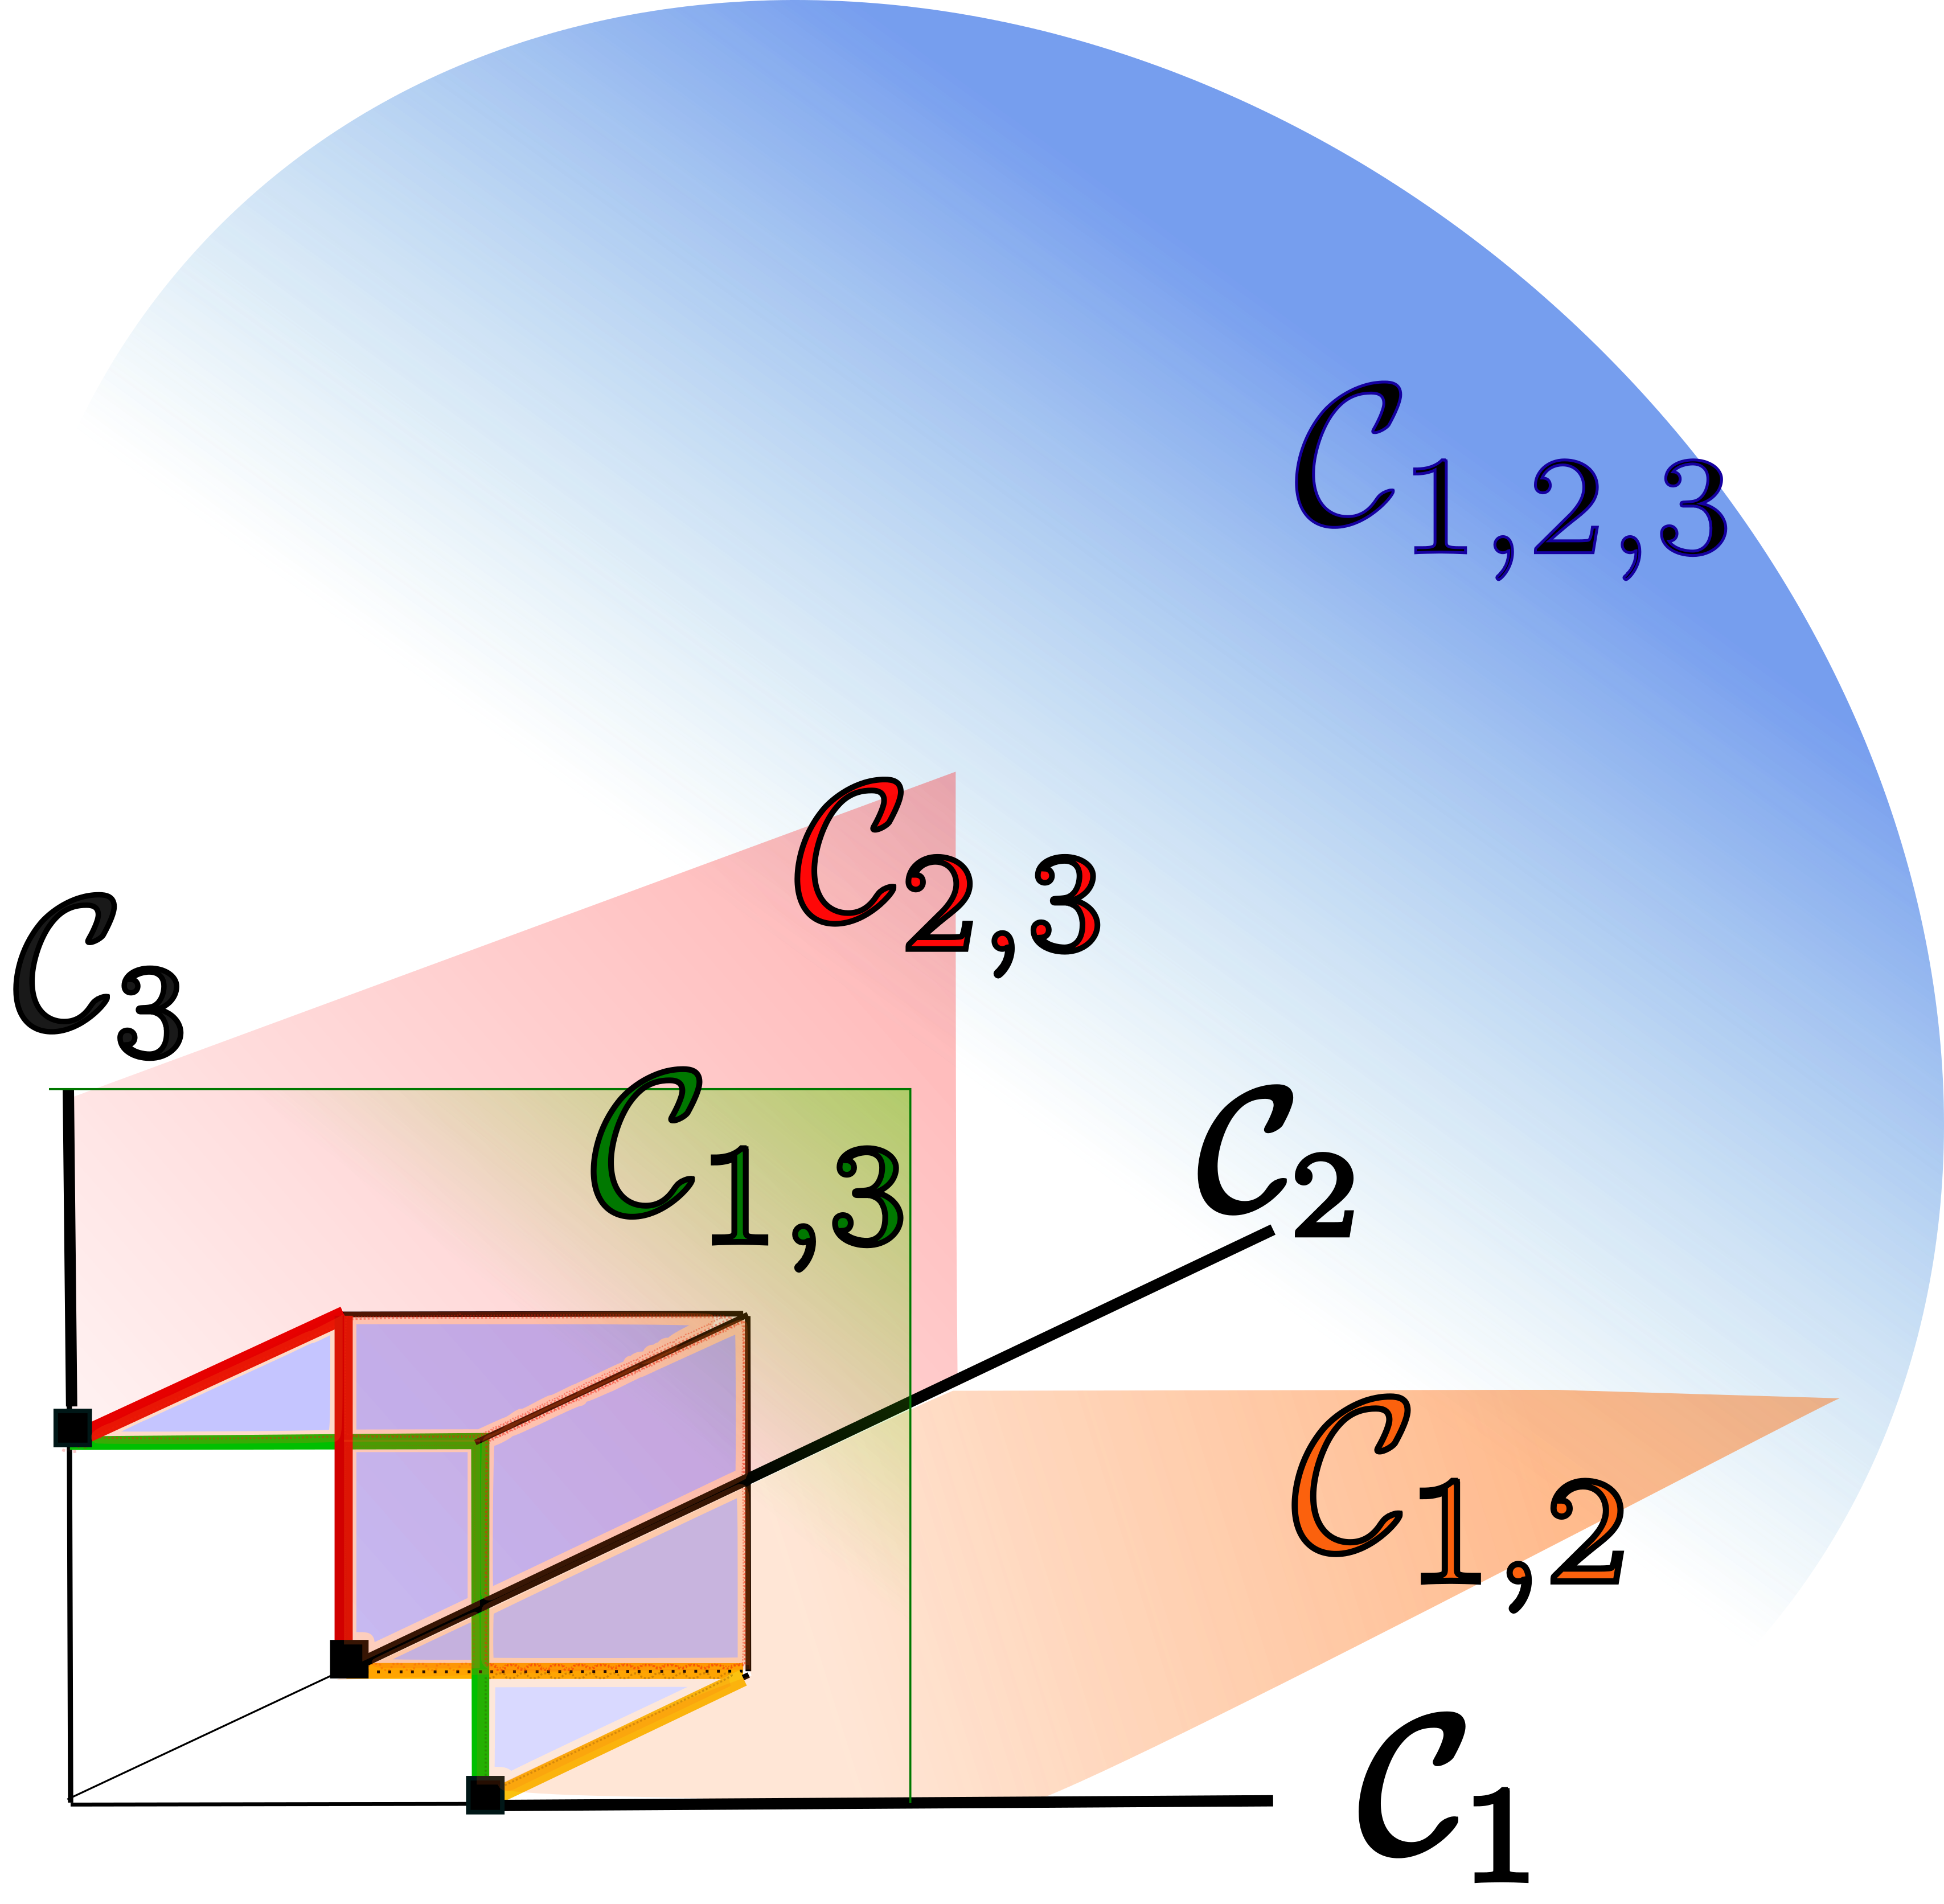
\includegraphics[scale=0.2]{fig_source/cone}
\captionof{figure}{Truncated cones in 3D}
\label{jmva:fig:3Dcones}
\end{minipage}\hfill
\begin{minipage}{0.5\linewidth}
\centering
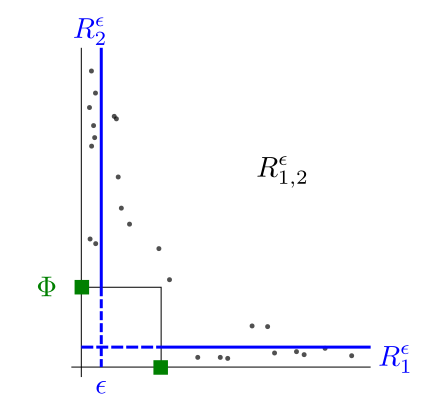
\includegraphics[width=0.64\linewidth]{fig_source/representation2D}
\captionof{figure}{Truncated $\epsilon$-rectangles in 2D}
\label{jmva:2Dcones}
\end{minipage}


\begin{lemma}\label{jmva:lem:limit_muCalphaEps}
For any non empty index subset $\emptyset \neq \alpha\subset\{1,\ldots,d\}$, the exponent measure of
$\cone_\alpha$ is
\[
\mu(\cone_\alpha) = \lim_{\epsilon\to 0} \mu(R_\alpha^\epsilon).
\]
\end{lemma}
\begin{proof}
First consider the case $\alpha=\dd$. Then $R_\alpha^\epsilon$'s forms an increasing sequence of sets as $\epsilon$ decreases and $\mathcal{C}_\alpha = R_\alpha^0 = \cup_{\epsilon>0, \epsilon \in \mathbb{Q}}~R_\alpha^\epsilon$. The result follows from the `continuity from below' property of the measure $\mu$. 
Now, for $\epsilon\ge 0$ and $\alpha\subsetneq\{1,\; \ldots,\; d\}$, consider the sets
\begin{align}
O_\alpha^\epsilon &  =\{ \mb x \in\rset_+^d~: \forall j \in \alpha:x_j > \epsilon \},  \nonumber \\
N_\alpha^\epsilon &  =\{\mb x \in\rset_+^d~: \forall j \in \alpha:   x_j > \epsilon, \exists j \notin\alpha: x_j > \epsilon \}, \nonumber
\end{align}
so that $N_\alpha^\epsilon \subset O_\alpha^\epsilon$ and $R_\alpha^\epsilon  = O_\alpha^\epsilon \setminus N_\alpha^\epsilon$. Observe also that $\cone_\alpha = O_\alpha^0\setminus N_\alpha^0$. Thus, $\mu(R_\alpha^\epsilon) = \mu(O_\alpha^\epsilon) - \mu(N_\alpha^\epsilon)$, and $\mu(\cone_\alpha) = \mu(O_\alpha^0) - \mu(N_\alpha^0)$,  so that it is sufficient to show that 
\begin{align}
\mu(N_\alpha^0) = \lim_{\epsilon\to 0}\mu(N_\alpha^\epsilon) ,
\quad \text{and}  \quad
\mu(O_\alpha^0) = \lim_{\epsilon\to 0}\mu(O_\alpha^\epsilon). \nonumber
\end{align}
Notice that the $N_\alpha^\epsilon$'s and the $O_\alpha^\epsilon$'s form two increasing sequences of sets (when $\epsilon$ decreases), and that  $N_\alpha^0 = \bigcup_{\epsilon>0,\epsilon\in\mathbb{Q}} N_\alpha^\epsilon$, $O_\alpha^0 = \bigcup_{\epsilon>0,\epsilon\in\mathbb{Q}} O_\alpha^\epsilon$. This proves the desired result.
\end{proof}


%Equipped with Lemma~\ref{jmva:lem:limit_muCalphaEps}, 

We may now  make precise the  above heuristic
interpretation of the quantities $\mu(\cone_\alpha)$: the vector
$\mathcal{M}=\{ \mu(\mathcal{C}_{\alpha}):\; \emptyset \neq
\alpha\subset\{1,\; \ldots,\; d \}\}$ asymptotically describes the
dependence structure of the extremal observations. 
% Equipped with Lemma~\ref{jmva:lem:limit_muCalphaEps}, the meaning of the
% statement 
% `$\mu(\cone_\alpha) > 0$' becomes clear. 
%
% Indeed, since the
% boundaries of the sets $\Omega_\alpha^\epsilon$ (viewed as subsets of
% $\mathbb{S}_\infty^{d-1}$) are disjoint, only a countable number of them may be
% discontinuity sets of $\Phi$. Thus, by homogeneity, the 
%  number of the sets $\cone_\alpha^\epsilon$ which are discontinuity
% sets of $\mu$ is at most countable. Hence, the threshold $\epsilon$ may be chosen arbitrarily small (so that, by
% Lemma~\ref{jmva:lem:limit_muCalphaEps}, $\mu(\cone_\alpha^\epsilon)$ is
% arbitrarily close to $\mu(\cone_\alpha)$), in such a way that
% $\cone_\alpha^\epsilon$ is a continuity set of $\mu$, 
Indeed, by
Lemma~\ref{jmva:lem:limit_muCalphaEps}, and the discussion above, $
\epsilon$ may be chosen such that $R_\alpha^\epsilon$ is a
continuity set of $\mu$, while $\mu(R_\alpha^\epsilon)$ is
arbitrarily close to $\mu(\cone_\alpha)$.  Then, using the
characterization (\ref{jmva:eq:regularVariation}) of  $\mu$, 
the following asymptotic identity  holds true:
\begin{align}
\lim_{t\to\infty} t \PP\left( \|\mb V\|_\infty\ge t, V^j> \epsilon t~~ (j \in\alpha), V^j \le \epsilon t~~ (j\notin\alpha)\right) &=\mu(R_\alpha^\epsilon) \\ \nonumber
 &\simeq \mu(\cone_\alpha). \nonumber
\end{align}
\begin{remark}
  \label{jmva:rk_approx_mu_n}
In terms of conditional probabilities, denoting $R = \|T(\mb X)\|$, where
  $T$ is the standardization map $\mb X\mapsto \mb V$,  we have
\begin{align}
\nonumber  \PP(T(\mb X)\in r R_\alpha^\epsilon~|~ R>r) = 
\frac{r \PP(\mb V\in r R_\alpha^\epsilon)}{ r\PP(\mb V \in r([\mb 0,\mathbf{1}]^c)} \xrightarrow[r\to\infty]{}\frac{\mu(R_\alpha^\epsilon)}{\mu([\mb 0,\mathbf{1}]^c)},
\end{align}
 as in~\eqref{jmva:eq:limitConditAngle}. In other terms, 
\begin{align}
\PP\left( V^j> \epsilon r~~ (j \in\alpha), V^j \le \epsilon r~~ (j\notin\alpha) ~\big\vert~ \|\mb V\|_\infty\ge r \right) &\xrightarrow[r\to\infty]{} C \mu(R_\alpha^\epsilon) \\ \nonumber
&~~~~~\simeq C\mu(\cone_\alpha), \nonumber
\end{align}
where $C = 1/ \Phi(S_\infty^{d-1}) =1/\mu([\mb 0,\mathbf{1}]^c) $.
This clarifies the meaning of `large' and `small' in the heuristic
explanation given above. 
\end{remark}

\noindent {\bf Problem statement.} % The goal of this paper is to estimate the dependence structure of the $d$-dimensional heavy-tailed r.v. $X$ in extreme
% regions from i.i.d. observations.
As explained above, our goal is to  describe the dependence on extreme
regions by investigating the structure of $\mu$ (or, equivalently,
that of $\Phi$). % , which is determined
% by that of the spectral measure $\Phi$.
More precisely, the aim is twofold. First, recover a rough
approximation of the support of $\Phi$ based on the partition
$\{\Omega_\alpha, \alpha\subset\{1,\ldots,d\}, \alpha\neq
\emptyset\}$, that is, determine which $\Omega_\alpha$'s have
nonzero mass, or equivalently, which $\mu_\alpha's$ (\emph{resp.}
$\Phi_\alpha$'s) are nonzero. This support estimation is potentially
sparse (if a small number of $\Omega_\alpha$ have non-zero mass) and
possibly low-dimensional (if the dimension of the sub-cones
$\Omega_\alpha$ with non-zero mass is low).
%a well chosen partition of the input space, 
The second objective is to 
investigate how the exponent measure $\mu$ spreads its mass on the
$\mathcal{C}_{\alpha}$'s, the theoretical quantity
$\mu(\mathcal{C}_{\alpha})$ indicating to which extent extreme
observations may occur in the `direction' $\alpha$ for $\emptyset
\neq \alpha \subset \{1,\; \ldots,\; d \}$. 
%  estimate the amount of angular mass
% $\mu(\cone_\alpha) = \Phi(\Omega_\alpha)$  on each non-void element of the
% partition.
These two goals are achieved using empirical versions of
the angular measure defined in
Section~\ref{jmva:sec:classicEstimators}, evaluated on the
$\epsilon$-thickened rectangles $R_\alpha^\epsilon$.
% This problem can be tackled by investigating how the exponent measure
% $\mu$ spreads its mass on the $\mathcal{C}_{\alpha}$'s, the
% theoretical quantity $\mu(\mathcal{C}_{\alpha})$ indicating to which
% extent extreme observations may occur in the `direction' $\alpha$ for
% $\emptyset \subsetneq \alpha \subset \{1,\; \ldots,\; d \}$.
Formally, we wish to recover the $(2^{d}-1)$-dimensional unknown
vector 
\begin{align}
\label{jmva:eq:representation_M}
\mathcal{M}=\{ \mu(\mathcal{C}_{\alpha}):\; \emptyset \neq \alpha\subset\{1,\; \ldots,\; d \}\}
\end{align}
 from $\mb X_1,\;
\ldots,\; \mb X_n\overset{i.i.d.}{\sim} \mb F$ and build an estimator
$\widehat{\mathcal{M}}$ such that
\begin{align}
\nonumber
\vert\vert \widehat{\mathcal{M}} -\mathcal{M}
\vert\vert_{\infty} \;%\overset{def}
{=} \; \sup_{\emptyset \neq \alpha \subset \{1,\; \ldots,\; d \}}\; \vert
\widehat{\mathcal{M}}(\alpha)- \mu(\mathcal{C}_{\alpha})\vert
\end{align}
is small with large probability.  % As $\mu(\mathcal{C}_{\alpha})=\Phi(\Omega_{\alpha})$ for any $\alpha$ and
In view of Lemma~\ref{jmva:lem:limit_muCalphaEps}, (biased) estimates of
$\mathcal{M}$'s components are built from an empirical version of 
the exponent measure, evaluated on the
$\epsilon$-thickened rectangles $R_\alpha^\epsilon$ (see Section~\ref{jmva:sec:classicEstimators} below). As a by-product, one obtains an estimate of the support of the limit measure $\mu$,
\begin{align}
\bigcup_{\alpha:\; \widehat{\mathcal{M}}(\alpha)>0 }\mathcal{C}_{\alpha}. \nonumber
\end{align}
 The results stated in the next section are non-asymptotic and sharp bounds are given by means of {\sc VC} inequalities tailored to low probability regions.
%, which is determined
%by that of the spectral measure $\Phi$. 
%More precisely,  the aim is
%twofold: first, recover a rough approximation of the support of
%$\Phi$ based on  the partition $\{\Omega_\alpha,
%\alpha\subset\{1,\ldots,d\}, \alpha\neq \emptyset\}$, that is,
%determine which $\Omega_\alpha$'s have nonzero mass, or equivalently,
%which $\mu_\alpha's$ (\emph{resp.} $\Phi_\alpha$'s) are nonzero; 
%a well chosen partition of the input space, 
%second, estimate the amount of angular mass
%$\mu(\cone_\alpha) = \Phi(\Omega_\alpha)$  on each non-void element of the
%partition.  These two goals are achieved using empirical versions of
%the angular measure defined in
%section~\ref{jmva:sec:nonParamEstimators}, evaluated on the
%$\epsilon$-thickened cones $\cone_\alpha^\epsilon$. Non-asymptoitc upper bounds on 
%the error are derived in section~\ref{jmva:sec:estimation} using VC
%inequalities adapted to low probability regions. 


\subsection{Regularity Assumptions}\label{jmva:sec:RegularAssumptions} % and Further Notations}
Beyond the existence of the limit measure $\mu$ (\ie~multivariate regular variation of $\mathbf{V}$'s distribution, see~\eqref{jmva:intro:regvar}), and thus, existence of an angular measure $\Phi$ (see (\ref{jmva:mu-phi})),
three additional assumptions are made, which are natural when estimation of the support of a distribution is considered. 

\begin{assumption}\label{jmva:hypo:continuous_margins}
The margins of $\mb X$ have continuous c.d.f., namely $F_j,~1 \le j \le d$ is continuous.
\end{assumption}
\noindent
 Assumption~\ref{jmva:hypo:continuous_margins}
is widely used in the context of non-parametric estimation of the dependence
structure (see \emph{e.g.} \cite{Einmahl2009}): it ensures that the transformed variables $V^j = (1 -
F_j(X^j))^{-1}$ (\emph{resp.} $U^j =  1 -F_j(X^j)$) have indeed a
standard Pareto distribution, $\P(V^j>x) = 1/x,~ x\ge 1$ (\emph{resp.}
the $U^j$'s are uniform variables). 

\bigskip
For any non empty subset $\alpha$ of $\{1,\; \ldots,\;d\}$, one denotes by $\ud x_\alpha$ the Lebesgue measure on ${\cal C}_\alpha$ and write $\ud x_\alpha  = \ud x_{i_1}\ldots\ud x_{i_k}$, when $\alpha=\{i_1, \ldots , i_k\}$. For convenience, we also write $\ud x_{\alpha\setminus{i}}$ instead of  $\ud x_{\alpha\setminus{\{i\}}}$.
% \begin{align*}
%   \mathcal{C}_\alpha^\epsilon = \{  \|x\| \ge 1: &\frac{x_i}{\|x\|_\infty} > \epsilon \text{ for }
%   i\in\alpha, \\
% &\frac{x_i}{\|x\|_\infty}\le\epsilon \text{ for } i\notin \alpha \quad \}~.
% \end{align*}
\begin{assumption}\label{jmva:hypo:continuousMu}
Each component $\mu_\alpha$ of~\eqref{jmva:eq:decomp1} is absolutely continuous w.r.t.
Lebesgue measure $\ud x_\alpha$ on ${\cal C}_\alpha$. %This implies that $\Phi_\alpha$ is absolutely continuous with respect to the Lebesgue measure on $\Omega_\alpha$. It is also assumed that, each of the induced densities is bounded.
\end{assumption}
\noindent
% For $\alpha\subset \{1,\ldots ,d\}$,  $\alpha\neq
% \emptyset$, the subset of the sphere corresponding to the cones is
% \begin{align*}
% \Omega_{\alpha} & = \{x \in S_{\infty}^{d-1} :  x_i > 0 \text{ for } i\in\alpha~,~  x_i = 0 \text{ for } i\notin \alpha   \} \\
% & = S_{\infty}^{d-1}\cap {\mathcal{C}}_\alpha ~ .
% \end{align*}
% \noindent
% Thus, the $\Omega_\alpha $'s form  a partition of $S_\infty^{d-1}$, and we have 
% \begin{align*}
% \mu(\mathcal{C}_i) ~=~  \Phi(\Omega_i) \text{ ~~~and~~~ } \Phi ~=~ \sum_{\emptyset \subsetneq \alpha\subset\{1,\ldots ,d\}} \Phi_\alpha ~,
% \end{align*}  
% \noindent
% where $\Phi_\alpha$ denotes the restriction of $\Phi$ to $S_{\infty}^{d-1} \cap {\Omega}_\alpha$.
Assumption~\ref{jmva:hypo:continuousMu} has a very convenient consequence 
regarding $ \Phi$: the fact that the exponent measure $\mu$ spreads no mass on subsets of the form 
$\{\mb x: \;\ninf{\mb x} \ge 1, x_{i_1} = \dotsb =  x_{i_r} \neq 0 \}$ with $r \ge 2$,
implies that the spectral measure $\Phi$ spreads no mass on edges $\{\mb x: \;\ninf{\mb x} = 1,  \; x_{i_1} = \dotsb =  x_{i_r} =1 \}$ with $r \ge 2~.$
This is summarized by the following result.
\begin{lemma}\label{jmva:lem:continuousPhi}
Under Assumption~\ref{jmva:hypo:continuousMu}, the following assertions holds true.
\begin{itemize}
\item  $ \Phi$ is concentrated on the (disjoint) edges
\begin{align}
   \Omega_{\alpha,i_0} = \{\mb x: \; \ninf{\mb x}  = 1,\; x_{i_0} = 1,~~& 0<  x_i < 1 ~~\text{~for~} i \in \alpha \setminus \{i_0\}\\ \nonumber
&x_i=0 ~~~~\text{~~~ for } i\notin \alpha ~~~~~~~\} \nonumber
\end{align}
for $i_0\in\alpha$, $\emptyset \neq \alpha\subset\{1,\; \ldots,\; d \}$.
\item The restriction $\Phi_{\alpha,i_0}$ of $\Phi$ to
  $\Omega_{\alpha,i_0}$ is absolutely continuous \wrt~the Lebesgue measure $\ud x_{\alpha\setminus{i_0}}$ on the cube's edges, whenever $|\alpha|\ge 2 $.

\end{itemize}
\end{lemma}
\begin{proof}
  The first assertion straightforwardly results from the discussion above.  Turning to the
  second point, consider any  measurable
  set $D \subset \Omega_{\alpha,i_0}$ such that $\int_{D}\ud x_{\alpha \setminus i_0} = 0$. Then the
  induced truncated cone $\tilde D = \{ \mb v:~ \|\mb v\|_\infty \ge
  1, \mb v / \|\mb v\|_\infty \in D \}$ satisfies $\int_{\tilde D}\ud
  x_{\alpha} = 0$ and belongs to $\mathcal{C}_\alpha$. Thus,  by virtue of
  Assumption~\ref{jmva:hypo:continuousMu}, $\Phi_{\alpha,
    i_0}(D)=\Phi_{\alpha}(D) = \mu_\alpha(\tilde D) = 0$.
\end{proof}

\noindent
It follows from Lemma~\ref{jmva:lem:continuousPhi} that the angular
measure $\Phi$ decomposes as $\Phi = \sum_{\alpha} \sum_{i_0\in\alpha}
\Phi_{\alpha,i_0}$  and that there exist densities $ \frac{\ud
  \Phi_{\alpha,i_0}}{\ud x_{ \alpha \smallsetminus i_0}},~~
|\alpha|\ge 2,~i_0\in\alpha,$ such that for all $B \subset
\Omega_\alpha,~~ |\alpha| \ge 2$,
\begin{align}
\label{jmva:eq:decomposePhi}
\Phi(B)~=~ \Phi_\alpha(B)~=~ \sum_{i_0\in\alpha} \int_{B\cap \Omega_{
    \alpha,i_0} } \frac{\ud \Phi_{\alpha,i_0}}{\ud x_{ \alpha
    \smallsetminus i_0}}(x) \ud x_{\alpha\setminus i_0}. 
\end{align}
% In view of equation~\eqref{jmva:eq:decomposePhi},  in particular, 
% \begin{lemma}
% Each $\Phi_{\alpha,i_0}$ is continuous with respect to $\ud x_i$, for
% $i\in\alpha \setminus \{i_0\}$ .
% \end{lemma}
In order to formulate the next assumption, for $|\beta| \ge 2$, we set
\begin{align}
\label{jmva:eq:supDensity}
M_\beta = % \sup_{i,j \in\beta,~ j\neq i} ~~~~\sup_{x\in\Omega_{\beta,i}} ~~~~ \frac{\ud  \Phi_{\beta, i}}{\ud x_j}(x)  ~~??=??~
~ \sup_{i \in\beta} ~~\sup_{x\in\Omega_{\beta,i}} ~~~~ \frac{\ud  \Phi_{\beta, i}}{\ud x_{\beta \setminus i}}(x).
\end{align}


\begin{assumption}\label{jmva:hypo:abs_continuousPhi}({\sc Sparse Support})
  The angular density is uniformly bounded on $S^{d-1}_\infty$ ($\forall |\beta| \ge 2,~M_\beta < \infty$), and there exists a constant  $M>0$, such that we have $\sum_{|\beta| \ge 2} M_\beta < M$, where the sum is over subsets $\beta$ of $\{1,\ldots,d\}$ which contain at least two elements.
\end{assumption}

\begin{remark}
The constant $M$ is problem dependent. However, in the case where our representation $\mathcal{M}$ defined in \eqref{jmva:eq:representation_M} is the most informative about the angular measure, that is, when the density of $\Phi_\alpha$ is constant on $\Omega_\alpha$, we have $M \le d$: Indeed, in such a case, 
$M \le \sum_{|\beta| \ge 2} M_\beta |\beta| = \sum_{|\beta| \ge 2} \Phi(\Omega_\beta) \le \sum_\beta \Phi(\Omega_\beta) \le \mu([\mb 0,\mb 1]^c)$.
% An order of magnitude for the value of $M$ is given as follows. Assuming that $\Phi$ has constant density on each sub-sphere $\Omega_\alpha$, then
% $\mu([\mb 0,\mb 1]^c) = \sum_\beta \Phi(\Omega_\beta) \ge \sum_{|\beta| \ge 2} \Phi(\Omega_\beta) = \sum_{|\beta| \ge 2} M_\beta |\beta| $.
The equality inside the last expression comes from the fact that the Lebesgue measure of a sub-sphere $\Omega_\alpha$ is $|\alpha|$, for $|\alpha| \ge 2$. Indeed, using the notations defined in Lemma~\ref{jmva:lem:continuousPhi}, $\Omega_\alpha = \bigsqcup_{i_0 \in \alpha}\Omega_{\alpha,i_0}$, each of the edges $\Omega_{\alpha,i_0}$ being unit hypercube. % (Intuitively, in dimension 3, $\Omega_{\{1,2,3\}}$ is a cube whose 3 faces corresponding to the positive quadrant are unit squares).
Now, $\mu([\mb 0,\mb 1]^c) \le \mu(\{v,~ \exists j,~ v_j > 1\} \le d \mu(\{v,~v_1 >1\})) \le d$.
% Noting that the Lebesgue measure of a sub-sphere $\Omega_\alpha$ is $|\alpha|$, if $\Phi$ is constant on each sub-sphere we have
% $\mu([\mb 0,\mb 1]^c) = \sum_\beta \Phi(\Omega_\beta) \ge \sum_{|\beta| \ge 2} \Phi(\Omega_\beta) = \sum_{|\beta| \ge 2} M_\beta |\beta| $

\noindent
Note that the summation $\sum_{|\beta| \ge 2} M_\beta |\beta|$ is smaller than $d$ despite the (potentially large) factors $|\beta|$. Considering $\sum_{|\beta| \ge 2} M_\beta$ is thus reasonable: in particular, $M$ will be small when only few $\Omega_\alpha$'s have non-zero $\Phi$-mass, namely when the representation vector $\mathcal{M}$ defined in \eqref{jmva:eq:representation_M} is sparse.
\end{remark}
\noindent Assumption~\ref{jmva:hypo:abs_continuousPhi} is naturally involved in the derivation of upper bounds on the error made when approximating $\mu(\cone_\alpha)$ by the empirical counterpart of $\mu(R_\alpha^\epsilon)$.
The estimation error bound derived in Section~\ref{jmva:sec:estimation} depends on the sparsity constant $M$.

%XXX commments on these assumptions
% \begin{assumption}\label{jmva:hypo:M}
% For every $\beta$ such that $|\beta| > 2$,~ $M_\beta$ is finite and $|\beta_1| \le |\beta_2| \Rightarrow M_{\beta_1} \ge M_{\beta_2}$.
% \end{assumption}
% One 'parcimony assumption' would be something like $M_\beta\le e^{-|\beta|}$.

% In other words we select, for each feature $j\le d$, the `$k$ largest values' $X_i^j$
% over the $n$ observations. According to the nature of the extremal dependence,
% a number between $k$ and $dk$ of observations are selected: $k$ in
% case of perfect dependence, $dk$ in case of `asymptotic independence', which
% means, in EVT, that the components may only be large one at a time. In
% any case, the number of observations considered as extreme is proportionnal to $k$, whence the normalizing factor $\frac{n}{k}$. 

%


% Yet the goal is to study the dependence between the $V_i^j$, $i$ fixed anf $j$ varying.
% One way to proceed is to characterize, for each subset of features
% $\alpha \subset \{1,...,d\}$, the `correlation' of these features
% given that one of them at least  is large and the others are small. %extreme (\ie~given that the observation is extreme).
% Formally, we  associate to each such $\alpha$ a coefficient
% $\mu_n^\alpha$ reflecting the degree of dependence between the
% features $\alpha$. Theoretically, by definition of asymptotic
% dependence, this coeficient is to be proportional to the expected number of
% points $V$ verifying $V^j > 0$, $j \in \alpha$ and $V^j = 0,~ j\notin
% \alpha$, and $\|V\|_\infty\ge r$, namely $ r^{-1}V \in \mathcal{C}_\alpha$ with 
% \begin{align}
% %\label{jmva:cone}
% \mathcal{C}_\alpha = \{v \ge 0,~\|v\|_\infty \ge 1,~ v_j > 0 ~\text{ for } j \in \alpha,~ v_j = 0 ~\text{ for } j \notin \alpha \}.
% \end{align}
% (see Fig.~\ref{jmva:fig:3Dcones}) But in practice, the data are non-asymptotic so that if $\alpha \neq \{1,\ldots,d\}$ the cones $\mathcal{C}_\alpha$ have zero Lebesgue measure and are not likely to receive empirical mass. Consider then a tolerance parameter $\epsilon>0$ and approximate the asymptotic mass of $~\mathcal{C}_\alpha~$ by the non-asymptotic mass of 
% \begin{align}
%  \label{jmva:eq:epsilonCone}
%  ~\mathcal{C}_\alpha^\epsilon~=\{v \ge
%  0,~\|v\|_\infty \ge 1,~ v_j > \epsilon \|v\|_\infty ~\text{ for } j
%  \in \alpha,~v_j \le \epsilon\|v\|_\infty ~\text{ for } j \notin \alpha
%  \} ,
% \end{align}
% which leads to coefficients 

% This motivates the study of the \stdf $l$, since it is now theoretically clear how the asymptotic tail dependence structure of $F$ is contained in $l$.
% XXXXXXXXXXXXXXXXXXXXXXXXXXXXXXXXXXXXXXXXXXXXXXXXXXXXXXXXXXXXXXXXXXXXXXXXXXXXXXXXXXXXXXXXXXXXXXXX
% % The measures $\mu$ and $\Lambda$ are called exponent measures and have the following properties:
% % \begin{itemize}
% % \item standardized marginals: for all $a>0$,
% % \begin{align*}
% % \Lambda([0,a]\times[0,\infty]^{d-1})~=~\Lambda([0,\infty]&\times[0,a]\times[0,\infty]^{d-2})
% % \\&~=~...~=~\Lambda([0,\infty]^{d-1}\times[0,a])~=~a
% % \end{align*}
% % \noindent and
% % \begin{align*} 
% % \mu([a,\infty]\times[0,\infty]^{d-1})~=~\mu([0,\infty]&\times[a,\infty]\times[0,\infty]^{d-2})
% % \\&~=~...~=~\mu([0,\infty]^{d-1}\times[a,\infty])~=~a^{-1}
% % \end{align*}
% % \item homogeneity: $\Lambda(c.)=c~ \Lambda(.)$ and $\mu(c.)=c^{-1} \mu(.)$
% % \item concentration: $\Lambda$, $\mu$ are respectively concentrated on $(0,\infty]^d \setminus \{\infty\}$, $[0,\infty)^d \setminus \{0\}$
% % \end{itemize}
% The homogeneity property yields a decomposition of $\mu$ into a
% radial and angular part (see de Haan and Resnick ...). 

\section{A non-parametric estimator of the subcones' mass : definition and preliminary results}
\label{jmva:sec:estimation}

In this section, an estimator $\widehat{\mathcal{M}}(\alpha)$ of each of the sub-cones' mass
$\mu(\cone_\alpha)$, $\emptyset\neq\alpha\subset\dd$, is
  proposed, based on observations  $\mb X_1,.\ldots, \mb X_n$, \iid~copies of $\mb X\sim \mb F$.
Bounds on the error $\vert\vert
  \widehat{\mathcal{M}}-\mathcal{M}\vert\vert_{\infty}$ are
  established. In the remaining of this chapter, we work under
  Assumption~\ref{jmva:hypo:continuous_margins} (continuous margins, see
  Section~\ref{jmva:sec:RegularAssumptions}). 
Assumptions~\ref{jmva:hypo:continuousMu}~and~\ref{jmva:hypo:abs_continuousPhi}
are not necessary to prove a preliminary result on a class of
rectangles (Proposition~\ref{jmva:prop:g} and Corollary~\ref{jmva:cor:mu_n-mu}). However, they are required % to approximate cones with rectangles
% (Proposition~\ref{jmva:prop:mu_n-mu}) and
to bound the bias induced by the tolerance parameter
$\epsilon$ (in Lemma~\ref{jmva:lemma_simplex}, Proposition~\ref{jmva:prop_simplex} and in the main result, Theorem~\ref{jmva:thm-princ}).  
% under the hypotheses listed in Section~\ref{jmva:sec:RegularAssumptions}. %  , we next investigate the problem of estimating $\mathcal{M}$ based on observations  $\mb X_1,.\ldots, \mb X_n$, \iid copies of $\mb
% % X\sim F$.
\subsection{A natural empirical version of the exponent measure mu}
\label{jmva:sec:classicEstimators}
 Since the marginal distributions $F_j$ are unknown, we classically consider
the empirical counterparts of the $\mb V_i$'s, 
$\mb{\widehat  V}_i = (\widehat V_i^1, \ldots,\widehat
V_i^d)$, $1\le i\le n$, as standardized  variables obtained from a
rank transformation (instead of a probability integral
transformation),  
\[\mb{\widehat  V}_i = \left( ( 1- \widehat F_j
  (X_i^j))^{-1}\right)_{1 \le j \le d}~, \]
  where 
$\widehat F_j (x) = (1/n) \sum_{i=1}^n \mathbf{1}_{\{X_i^j < x\}}$.
%
We denote by $T$ (\emph{resp.} $\widehat T$) the standardization
(\textit{resp.} the empirical standardization), 
\begin{align}
\label{jmva:def:transform}
T(\mb x) = \left( \frac{1}{1- F_j (x^j)}\right)_{1\leq j\leq d}
\text{~~and~~}
\widehat T(\mb x) = \left( \frac{1}{1- \widehat F_j(x^j)}\right)_{1\leq j\leq d}. 
\end{align}
The empirical probability distribution of the rank-transformed data is then given by
\begin{align*}
\mathbb{\widehat P}_n=(1/n)\sum_{i=1}^n\delta_{\mb{\widehat{V}}_i}.
\end{align*}
Since for a $\mu$-continuity set $A$ bounded away from $0$,   $t~ \mathbb{P}\left( \mb V \in t A\right)  \to \mu(A)$ as $t \to \infty$, see~\eqref{jmva:eq:regularVariation}, a natural empirical version of $\mu$ is defined as 
\begin{align}\label{jmva:mu_n}
\mu_n(A) ~=~ \frac{n}{k} \widehat{\mathbb{P}}_n (\frac{n}{k}A) ~=~ \frac{1}{k}\sum_{i=1}^n \mathbf{1}_{\{\mb{\widehat{V}}_i \in \frac{n}{k} A\}}~.
\end{align}
 Here and throughout, we place ourselves in the asymptotic setting stipulating that $k = k(n) >0$ is such that $k \to \infty$ and $k = o(n)$ as $n \to \infty$.
The ratio $n/k$ plays the role of a large radial threshold.
Note that this estimator is commonly used in the field of
non-parametric estimation of the dependence structure, see \textit{e.g.}
\cite{Einmahl2009}. 


\subsection{Accounting for the  non asymptotic nature of  data:
  epsilon-thickening.}

 Since the cones $\mathcal{C}_\alpha$ have zero Lebesgue measure, 
and since, under Assumption~\ref{jmva:hypo:continuous_margins}, the margins are
continuous, the cones  are not likely to receive any empirical mass, 
 so that  simply counting points in $\frac{n}{k}\mathcal{C}_\alpha$ is not an
option: with probability one, only
the largest dimensional cone (the central one, corresponding to
$\alpha= \{1,\ldots,d\})$ will be hit. 
%
In view of Subsection~\ref{jmva:sec:decomposMu} and
Lemma~\ref{jmva:lem:limit_muCalphaEps}, 
 it is natural to introduce a 
tolerance parameter $\epsilon>0$ and to approximate the asymptotic mass
of $\mathcal{C}_\alpha$ with the non-asymptotic mass of
$R_\alpha^\epsilon$. We thus define the non-parametric estimator $\widehat{M}(\alpha)$ of
$\mu(\cone_\alpha)$ as
\begin{align}
\label{jmva:heuristic_mu_n}
\hatmass(\alpha) = \mu_n(R_\alpha^\epsilon), \qquad
\emptyset\neq\alpha\subset\dd.  %= \frac{n}{k} \mathbb{\hat P}_n \left ( \frac{n}{k} \mathcal{C}_\alpha^\epsilon \right),
\end{align}
%where $\mathbb{\hat P}_n=(1/n)\sum_{i=1}^n\delta_{\hat{V}_i}$ is the empirical probability distribution of the rank-transformed data.
Evaluating  $\hatmass(\alpha)$  boils down (see~\eqref{jmva:mu_n})
to counting points in $(n/k)\,R_{\alpha}^{\epsilon}$, as illustrated in Figure~\ref{jmva:estimation_rect}. The estimate $\hatmass(\alpha)$ is thus a (voluntarily
$\epsilon$-biased) natural estimator of $\Phi(\Omega_\alpha) = \mu(\mathcal{C}_\alpha)$.
\begin{figure}[!ht]
  \centering
  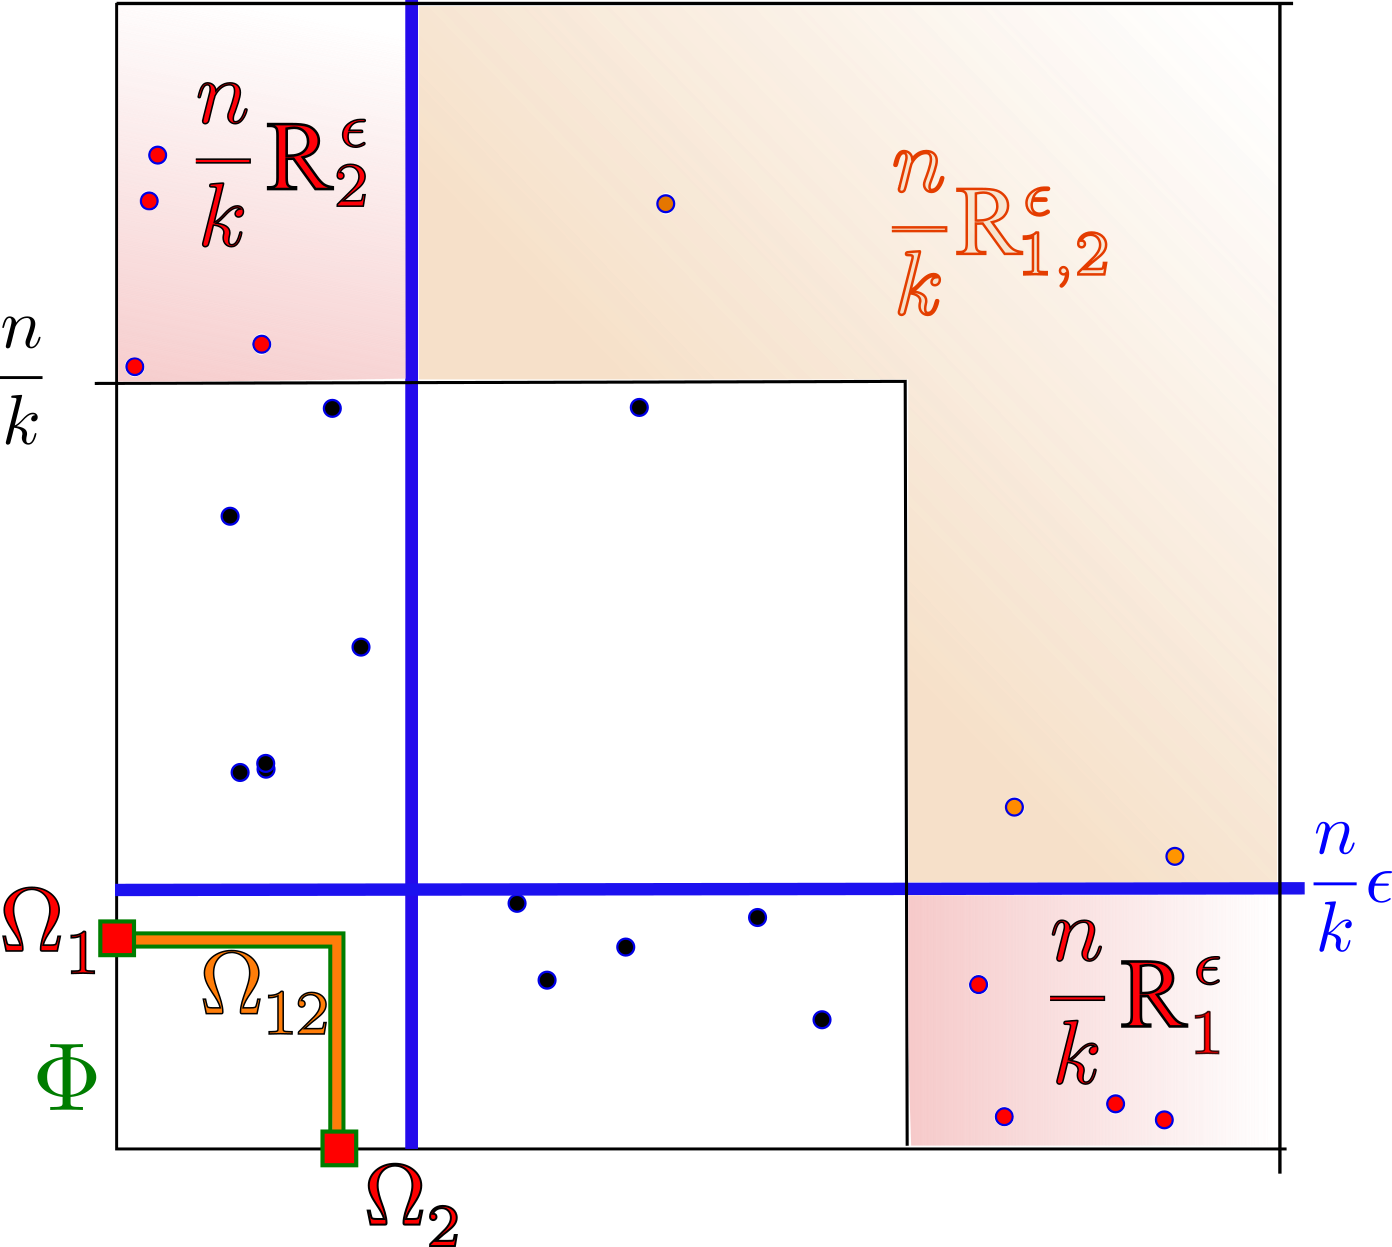
\includegraphics[width = 0.7\textwidth]{fig_source/representation2D_nk_rect.png}
  \caption{Estimation procedure}
  \label{jmva:estimation_rect}
\end{figure}


The coefficients $(\hatmass(\alpha))_{\alpha\subset\{1,\ldots,d\}}$ related to the cones $\mathcal{C}_\alpha$ constitute a summary representation of the dependence structure.  % constitute a   A representation of the dependence structure is then
% \begin{align}
% R_n(x) = \sum_{\alpha }\hatmass(\alpha) \mathds{1}_{\hat T(x) \in \mathcal{C}_\alpha^\epsilon},
% \end{align}
This representation is sparse as soon as the $\mu_n^{\alpha,  \epsilon}$ are positive only for a few groups of features $\alpha$ (compared to the total number of groups or sub-cones, $2^d$ namely). It is  is low-dimensional as soon as each of these groups $\alpha$ is of small cardinality, or equivalently the corresponding sub-cones are low-dimensional compared with $d$.

In fact, $\hatmass(\alpha)$ is (up to a normalizing constant) an empirical version of the  conditional probability that $T(\mb X)$ belongs to the rectangle $ r R_\alpha^\epsilon$, given that $\|T(\mb X)\|$ exceeds  a large threshold $r$. Indeed, as explained in Remark~\ref{jmva:rk_approx_mu_n},  
\begin{align}\label{jmva:eq:interprete_mun_Pcondit}
\mathcal{M}(\alpha) = \lim_{r \to \infty} \mu([\mb 0,\mathbf{1}]^c)~~\mathbb{P}(T(\mb X)\in r R_\alpha^\epsilon ~|~ \|T(\mb X)\|\ge r) . 
\end{align}

The remaining of this section is devoted to obtaining non-asymptotic upper bounds on the error $\vert\vert \widehat{\mathcal{M}}-\mathcal{M}\vert\vert_{\infty}$. 
The main result is stated in Theorem~\ref{jmva:thm-princ}. 
Before all, notice that the error may be obviously decomposed as the sum of a stochastic term and a bias term inherent to the $\epsilon$-thickening approach:
\begin{align}
\vert\vert \widehat{\mathcal{M}}-\mathcal{M}\vert\vert_{\infty} &~=~\max_{\alpha} |
\mu_n(R_\alpha^\epsilon)-\mu(\mathcal{C}_\alpha)|\nonumber
\\&~\le~ ~\max_\alpha |\mu-\mu_n|(R_\alpha^\epsilon) ~+~ \max_\alpha|\mu(R_\alpha^\epsilon)-\mu(\mathcal{C}_\alpha)|~.\label{jmva:error_decomp} 
\end{align}
Here and beyond, for notational convenience, we simply denotes `$\alpha$'  for `$\alpha$ non empty subset of $\{1,\; \ldots,\;d\}$'. The main steps of the argument leading to Theorem~\ref{jmva:thm-princ} are  as follows. First, obtain a uniform upper bound on the error $|\mu_n - \mu|$ restricted to a well chosen VC class of rectangles (Subsection~\ref{jmva:sec:rectangles}), and deduce an uniform bound on  $|\mu_n - \mu|(R_\alpha^\epsilon)$ (Subsection~\ref{jmva:sec:boundErrorEpsilonCones}). Finally, using the regularity assumptions (Assumption~\ref{jmva:hypo:continuousMu} and Assumption~\ref{jmva:hypo:abs_continuousPhi}), bound the difference $|\mu(R_\alpha^\epsilon) - \mu(\cone_\alpha)|$ (Subsection~\ref{jmva:sec:boundMuEpsilonCones}). 


\subsection{Preliminaries: uniform approximation over a VC-class of rectangles}
\label{jmva:sec:rectangles}
This subsection builds on the theory developed in Chapter~\ref{colt}, where a non-asymptotic bound is stated on the estimation of the stable tail dependence function (defined in~\eqref{back:stdf1}). % We prove here (Proposition~\ref{jmva:prop:g}) a generalized version of the result obtained by these authors. 
The \stdf $l$ is related to the class of sets of the form $[\mb 0, \mb v]^c$ (or $[\mb u, \boldsymbol{\infty}]^c$ depending on which standardization is used), and an equivalent definition is 
\begin{align}
\label{jmva:stdf}
l(\mathbf{x}):= \lim_{t \to \infty} t \tilde F (t^{-1}\mathbf{x}) = \mu([\mb 0, \mb x ^{-1}]^c) 
\end{align}
\noindent
with $\tilde F (\mathbf{x}) = (1-F) \big( (1-F_1)^\leftarrow(x_1),\ldots, (1-F_d)^\leftarrow(x_d)  \big)$.
 Here the notation
$(1-F_j)^\leftarrow(x_j)$ denotes the quantity $\sup\{y\,:\; 1-F_j(y) \ge x_j\}$. Recall that the marginally uniform variable $\mb U$ is defined by  $U^j = 1-F_j(X^j)$ ($1\le j\le d$). Then  in terms of standardized variables $U^j$, 
\begin{align}
\label{jmva:def:tildeF}
\tilde F(\mb x) = \P\Big(\bigcup_{j=1}^d\{U^j< x_j\}\Big) = \P(\mb
U\in [\mb x, \boldsymbol{\infty}[^c) = \P(\mb V \in [\mb 0, \mb x^{-1}]^c). 
\end{align}

A natural estimator of $l$ is its empirical version defined as
follows,  see \cite{Huangphd}, \cite{Qi97}, \cite{Drees98}, \cite{Einmahl2006}, \cite{COLT15}:
\begin{align}\label{jmva:empir-Stdf}
l_n(\mathbf{x}) &= \frac{1}{k}~\sum_{i=1}^{n} \mathds{1}_{\{ X_i^1 \ge
  X^1_{(n-\lfloor kx_1 \rfloor+1)}  \text{~~or~~} \ldots \text{~~or~~}
  X_i^d \ge  X^d_{(n-\lfloor kx_d\rfloor+1)}  \}}~.
\end{align}
The expression is indeed suggested by the definition of $l$ in  (\ref{jmva:stdf}), with all distribution functions and  univariate quantiles replaced by their empirical counterparts, and with $t$  replaced by $n/k$.
The following lemma allows to derive alternative expressions for the empirical version of the \stdf.  
\begin{lemma}
\label{jmva:lem:equivalence}
Consider the rank transformed variables 
$\mb{  \widehat U}_i = (\mb{ \widehat V}_i)^{-1} = ( 1- \widehat F_j
(X_i^j))_{1\leq j\leq d}$ for $i = 1, \ldots, n$. Then, for $(i,j)\in \{1,\ldots, n\}\times \{1,\ldots,d\}$,
with probability one,
$$
\widehat U_i^j \le \frac{k}{n} x_j^{-1} ~\Leftrightarrow~
\widehat V_i^j \ge \frac{n}{k} x_j ~\Leftrightarrow~
X_i^j \ge X_{(n-\lfloor  kx_j^{-1} \rfloor +1)}^j ~\Leftrightarrow~
U_i^j \le U_{(\lfloor kx_j^{-1}\rfloor)}^j~.
$$
\end{lemma}
The proof of Lemma~\ref{jmva:lem:equivalence} is standard and is provided in~\ref{jmva:appendix_proof} for completeness.
By Lemma~\ref{jmva:lem:equivalence}, the following alternative expression of $l_n(\mb x)$ holds true:
\begin{align}\label{jmva:empir-Stdf2}
l_n(\mb x)=\frac{1}{k} ~\sum_{i=1}^{n} \mathds{1}_{ \{U_i^1 ~\le~ U^1_{([kx_1])} \text{~~or~~} \ldots \text{~~or~~}  U_i^d ~\le~ U^d_{([kx_d])} \}}= \mu_n \left( [\mb 0, \mb x^{-1}]^c \right).
\end{align}
Thus, bounding the error $|\mu_n - \mu|([\mb 0,\mb x^{-1}]^c)$ is the same as
bounding $|l_n - l|(\mb x)$. 

Asymptotic properties of this empirical counterpart have been studied
in \cite{Huangphd}, \cite{Drees98}, \cite{Embrechts2000} and
\cite{dHF06} in the bivariate case, and \cite{Qi97},
\cite{Einmahl2012}. 
in the general multivariate
 case. 
In \cite{COLT15}, a non-asymptotic bound is established on the maximal deviation $$\sup_{0 \le \mb x \le T} |l(\mb x) - l_n(\mb x)|$$ for a fixed $T>0$, or equivalently on 
$$ \sup_{1/T \le \mb x } \left|\mu ( [\mb 0, \mb x]^c ) - \mu_n ( [\mb 0, \mb x]^c )\right|. $$
\noindent
The exponent measure $\mu$ is indeed easier to deal with when restricted to the class of sets of the form $[\mb 0, \mb x]^c$, which is fairly simple in the sense that it has finite VC dimension. % However we need to consider the restrictions of $\mu$ on a slightly more complex class which can better approximate the subcones $\mathcal{C}_\alpha^\epsilon$.






% Estimation of the angular measure, which involves sets that are more
% complex  than the rectangles are, has only been studied in dimension
% $2$ in \cite{Einmahl2009} who provide  asymptotic results 
% (asymptotic normality is stated by considering 2-dimensional regions
% hardly generalizable in larger dimension).
In the present work,  an important step is to bound the error on the
class of $\epsilon$-thickened rectangles $R_\alpha^\epsilon$. This is achieved by
using a more general class $R(\mb x, \mb z, \alpha, \beta)$, which includes (contrary to the collection of sets $[\mb 0,\mb x]^c$) the $R_\alpha^\epsilon$'s . 
This flexible class is defined by
\begin{align}
\nonumber R(\mb x, \mb z, \alpha, \beta) &~=~ \Big\{ \mb y \in [0, \infty]^d,
~~ y_j \ge x_j ~~\text{ for } j \in \alpha, 
\\&~~~~~~~~~~~~~~~~~~~~~~~~~~ y_j < z_j ~~\text{ for } j \in \beta \quad \Big\},
~~~  \mb x, \mb z \in [0, \infty]^{d}. \label{jmva:set-R}
\end{align}
Thus,
\begin{align*}
\mu_n \left( R(\mb x, \mb z, \alpha, \beta) \right) & ~=~ \frac{1}{k}
\sum_{i=1}^n \mathds{1}_{\{ \widehat V_i^j ~\ge~ \frac{n}{k} x_j  \text{ for } j \in \alpha \text{ ~and~ } \widehat V_i^j ~<~\frac{n}{k} x_j  \text{ for } j \in \beta \}}~.
\end{align*}

\noindent
Then, define the  functional $g_{\alpha,\beta}$ (which plays the same role as the \stdf) as follows:  
% For $ \mb a, \mb b \in [0, \infty]^d$, define the set $[\mb a, \mb b[$
% as 
% \[[\mb a, \mb b[~=~ \{x,~ a_j ~\le~ x_j ~<~ b_j, ~~\forall j \le d \}.\]
for $\mb x \in [0, \infty]^{d}\setminus\{\boldsymbol{\infty}\}$, $\mb z \in [0, \infty]^d$, $\alpha
\subset \{1,\ldots,d\} \setminus \emptyset$ and $\beta \subset
\{1,\ldots,d\}$, let
\begin{align}
&g_{\alpha, \beta}(\mb x, \mb z) ~~=~~ \lim_{t \to \infty} t \tilde
F_{\alpha, \beta}(t^{-1} \mb x, t^{-1} \mb z), \text{~~with}
\label{jmva:g-alpha} \\
&\tilde F_{\alpha, \beta}( \mb x,  \mb z) ~~=~~
 \mathbb{P} \left[ \left\{ U^j \le x_j ~~\text{ for } j \in \alpha
   \right\}~~\bigcap~~ \left\{U^j > z_j  ~~\text{ for } j \in\beta
   \right\}\right].
 \label{jmva:F-tilde-alpha}
\end{align}
 Notice that %  $g_{\alpha, \beta}(\mb
% x, \mb z)$ is a generalized version of the \stdf $l$ defined in
% \eqref{jmva:stdf1},  and
$\tilde F_{\alpha, \beta}( \mb x,  \mb z)$ is an extension of the
non-asymptotic approximation $\tilde F$ in~(\ref{jmva:stdf}).   % , see \cite{Qi97}.
By~(\ref{jmva:g-alpha}) and~\eqref{jmva:F-tilde-alpha}, we have 
\begin{align*}
  g_{\alpha, \beta}(\mb x, \mb z) &= \lim_{t \to \infty} t \mathbb{P}
  \left[ \left\{ U^j \le t^{-1} x_j ~\text{ for } j \in \alpha
    \right\}~\bigcap~ \left\{  U^j > t^{-1} z_j  ~\text{ for } j
      \in\beta \right\}\right] \\&= \lim_{t \to \infty} t \mathbb{P}
  \left[ \mb V \in t R(\mb x^{-1}, \mb z^{-1}, \alpha,~\beta) \right]~,
\end{align*}
 so that using~\eqref{jmva:eq:regularVariation},
\begin{align}\label{jmva:g_with_mu}
g_{\alpha, \beta}(\mb x, \mb z) = \mu([ R(\mb x^{-1}, \mb z^{-1}, \alpha,~\beta)]).
\end{align}




%Similarly to the way the standard tail dependence function $l$ is defined in (\ref{jmva:stdf}), namely $l(\mb x) =\lim_{t \to 0} t^{-1} \tilde F (tx) = \mu([0, \mb x^{-1}]^c)$, we define for $x \in [0, \infty)^{d}$, $z \in [0, \infty]^d$, $\alpha \subset \{1,\ldots,d\} \setminus \emptyset$ and $\beta \subset \{1,\ldots,d\}$ the functionnal 
%
The following lemma makes the relation between  $g_{\alpha,\beta}$ and  the angular measure
$\Phi$ explicit. Its proof is given in~\ref{jmva:appendix_proof}.
\begin{lemma}
\label{jmva:lem:g-alpha}
The function $g_{\alpha, \beta}$ can be represented as follows:
\begin{align*}
g_{\alpha, \beta}(\mb x, \mb z) = \int_{S^{d-1}} \left(\bigwedge_{j \in \alpha}{w_j x_j} - \bigvee_{j \in\beta} w_j z_j\right)_+~ \Phi(\ud \mb w)~,
\end{align*}
where $u\wedge v=\min\{ u,v \}$, $u\vee v=\max\{ u,v \}$ and $u_+=\max\{u, 0\}$ for any $(u,v)\in \mathbb{R}^2$.
\noindent
Thus, $g_{\alpha, \beta}$ is homogeneous and satisfies
\begin{align*}
|g_{\alpha, \beta}(\mb x, \mb z) - g_{\alpha, \beta}(\mb x', \mb z')| ~~\le~~  \sum_{j \in \alpha}|x_j - x_j'| ~+~  \sum_{j \in \beta}|z_j - z_j'|~,
\end{align*}
%where $C$ is an absolute constant (equal to the total mass of $\mu$ on $[\mb 0, \mb 1]^c$).
\end{lemma}
\begin{remark}
Lemma~\ref{jmva:lem:g-alpha} shows that the functional $g_{\alpha, \beta}$, which plays the same role as a  the \stdf, enjoys  a Lipschitz property.
\end{remark}
% From the representation 
% \begin{align*}
% h(x) = \int_{S^{d-1}} \min_j{w_j x_j} \phi(dw)
% \end{align*}
% $h$ is 1-Lipschitz and homogeneous as $l$

We now define the empirical counterpart of $g_{\alpha, \beta}$
(mimicking that of the empirical \stdf $l_n$ in (\ref{jmva:empir-Stdf}) ) by
%we define for $a,b \in [0,\infty]^d \setminus \infty$, again with the conventions $1/ \infty = 0$ and $1/0 = \infty$, the functionnal
\begin{align}
\label{jmva:def:gn}
g_{n, \alpha, \beta}(\mb x, \mb z) = \frac{1}{k}~\sum_{i=1}^{n}
\mathds{1}_{\{ X_i^j \ge X^j_{(n-\lfloor kx_j \rfloor+1)}  ~~\text{for}~
  j \in \alpha \text{~~~and~~~} X_i^j < X^j_{(n-\lfloor
    kx_j\rfloor+1)} ~~\text{for}~ j \in\beta \}}~.
\end{align}
As it is the case for the empirical \stdf (see~(\ref{jmva:empir-Stdf2})), $g_{n,\alpha,\beta}$ has an alternative expression
\begin{align}\label{jmva:eq:gn2}
  \nonumber g_{n, \alpha, \beta}(\mb x, \mb z)&=\frac{1}{k} ~\sum_{i=1}^{n}
  \mathds{1}_{\{ U_i^j ~\le~ U^j_{([kx_j])} ~~\text{for}~ j \in \alpha
    \text{~~~and~~~} U_i^j ~>~U^j_{([kx_j])} ~~\text{for}~ j \in\beta \}}\\
  &= \mu_n \left( R(\mb x^{-1}, \mb z^{-1}, \alpha,~\beta)\right),
\end{align}
where the last equality comes from the equivalence $\widehat V_i^j \ge \frac{n}{k} x_j \Leftrightarrow U_i^j \le U_{(\lfloor kx_j^{-1}\rfloor)}^j$ (Lemma~\ref{jmva:lem:equivalence}) and from the expression $\mu_n(\point) = \frac{1}{k}\sum_{i=1}^n \mathds{1}_{\mb{\widehat{V}}_i \in \frac{n}{k} (\point)}$, definition~\eqref{jmva:mu_n}.

% \subsubsection{A first result on the class $\left\{ R(\mb x, \mb z, \alpha, \beta),~  1/T \le \mb x, \mb z,~\alpha,\beta\right\}.$}
\noindent
The proposition below extends the result of \cite{COLT15}, by deriving an analogue upper bound on the maximal deviation 
$$% \sup_{ \substack{  0 \le \mb x, \mb z \le T \\ \alpha, \beta }}
\max_{\alpha,\beta}\sup_{ 0 \le \mb x, \mb z \le T} |g_{\alpha, \beta}(\mb x, \mb z) - g_{n, \alpha, \beta}(\mb x, \mb z)|~,$$ 
or equivalently on
$$\max_{\alpha, \beta}~ \sup_{1/T \le \mb x, \mb z } \left|\mu ( R(\mb x, \mb z, \alpha, \beta)) - \mu_n (R(\mb x, \mb z, \alpha, \beta) )\right| ~.$$
Here and beyond %for notational convenience 
we simply denote `$\alpha,\beta$'  for `$\alpha$ non-empty subset of $\{1,\ldots,d\}\setminus \emptyset$ and $\beta$ subset of
$\{1,\ldots,d\}$'. We also recall that comparison operators between two vectors (or
between a vector and a real number) are understood component-wise, \ie~ `$\mb x \le \mb z$' means `$x_j \le z_j$ for all $1\le j\le d$' and  for any real number $T$,  `$\mb x\le T$' means `$x_j \le T$ for all $1\le j\le d$'. 

\begin{proposition}
\label{jmva:prop:g}
Let $T \ge \frac{7}{2}(\frac{\log d}{k} + 1)$, and $\delta \ge e^{-k}$.  % For each $n >0$, with probability at least $1-\delta$,
% \begin{align*}
% \sup_{0 \le \mb x \le T} \left| l_n(\mb x) - l(\mb x) \right| ~\le~ Cd\sqrt{\frac{2T}{k}\log\frac{d+3}{\delta}} ~+~ \sup_{0 \le \mb x \le 2T}\left|\frac{n}{k} \tilde F(\frac{k}{n}\mb x)-\frac{n}{k} l ( \frac{k}{n} \mb x)\right|.
% \end{align*}
Then there is a universal constant $C$, such that for each $n>0$, with probability at least $1 - \delta$,%~ for each $\alpha \subset\{1,\ldots,d\}\setminus \emptyset$ and $\beta \subset\{1,\ldots,d\}$,
\begin{align}
\label{jmva:ineq:g}
\max_{\alpha, \beta} \sup_{ 0 \le \mb x, \mb z \le T } &\left| g_{n, \alpha, \beta}(\mb x, \mb z) - g_{\alpha, \beta}(\mb x, \mb z) \right| ~\le~  Cd\sqrt{\frac{2T}{k}\log\frac{d+3}{\delta}} 
\\\nonumber &~~~~~~~~~~~~~~~~~~~~~~~+ \max_{\alpha, \beta}  \sup_{0 \le \mb x, \mb z \le 2T}\left|\frac{n}{k} \tilde F_{\alpha, \beta}( \frac{k}{n} \mb x, \frac{k}{n} \mb z)- g_{\alpha, \beta}(\mb x, \mb z)\right|.
\end{align}
The second term on the right hand side of the inequality is an asymptotic bias term which goes to $0$ as $n \to \infty$ (see Remark~\ref{jmva:rk:bias}).
\end{proposition}
The proof follows the same lines as that of Theorem 6 in \cite{COLT15} and is detailed in \ref{jmva:appendix_proof}. Here is the main argument.

The empirical estimator is based on the empirical measure of `extreme' regions, which are hit only with  low probability. It is thus enough to bound maximal deviations on such low probability regions. The key consists in choosing an adaptive VC class which only covers the latter regions (after standardization to uniform margins), namely a VC class composed of sets of the kind $\frac{k}{n} R(\mb x^{-1}, \mb z^{-1}, \alpha, \beta)^{-1}$. In \cite{COLT15}, VC-type inequalities have been established that incorporate $p$, the probability of hitting the class at all. Applying these inequalities to the particular class of rectangles gives the result.

\subsection{Bounding empirical deviations over thickened rectangles}%$|\mu_n - \mu|(R_\alpha^\epsilon)$ uniformly over $\alpha$}
\label{jmva:sec:boundErrorEpsilonCones}
% In the previous subsection the quantity $\sup_{x > \frac{1}{T}}
% |\mu-\mu_n|(R(\mb x, \mb z, \alpha, \beta))$ has been bounded.
The aim of this subsection is to bound $|\mu_n - \mu|(R_\alpha^\epsilon)$ uniformly over $\alpha$ exploiting the previously established
bound on the deviations on rectangles, to obtain another uniform  bound for % We are
% now interested in bounding
$|\mu_n-\mu|(R_\alpha^\epsilon)$, for $\epsilon >0$ and $\alpha \subset \dd$. In the remainder of the chapter, $\bar \alpha$ denotes the complementary set of $\alpha$ in $\dd$.
Notice that directly from their definitions \eqref{jmva:eq:epsilon_Rectangle} and \eqref{jmva:set-R}, $R_\alpha^\epsilon$ and $R(\mb x, \mb z, \alpha, \beta)$ are linked by: 
\begin{align*}
R_\alpha^\epsilon = R(\boldsymbol \epsilon, \boldsymbol  \epsilon, \alpha, \bar \alpha) \cap [\mb 0, \mb 1]^c = R(\boldsymbol \epsilon, \boldsymbol  \epsilon, \alpha, \bar \alpha) \setminus R(\boldsymbol \epsilon, \boldsymbol{\tilde \epsilon}, \alpha, \{1,\ldots, d\})
\end{align*}
where $\boldsymbol{\tilde \epsilon}$ is defined by $\boldsymbol{\tilde \epsilon}_j = \mathds{1}_{j \in \alpha} + \epsilon \mathds{1}_{j \notin \alpha}$ for all $j \in \{1,\ldots,d\}$.
Indeed, we have: $R(\boldsymbol \epsilon, \boldsymbol  \epsilon, \alpha, \bar \alpha) \cap [\mb 0, \mb 1] = R(\boldsymbol \epsilon, \boldsymbol{\tilde \epsilon}, \alpha, \{1,\ldots, d\})$.
As a result, for $\epsilon < 1$,
$$\sup_{\epsilon \le \mb x, \mb z }|\mu_n-\mu|\left(R_\alpha^\epsilon\right) \le 2 \sup_{\epsilon \le \mb x, \mb z }|\mu_n-\mu|\left(R(\mb x,~ \mb z,~ \alpha,~ \bar \alpha)\right).$$
On the other hand, from~\eqref{jmva:eq:gn2} and \eqref{jmva:g_with_mu} we have 
\begin{align*}
\sup_{\epsilon \le \mb x, \mb z }|\mu_n-\mu|\left(R(\mb x,~ \mb z,~ \alpha,~ \bar \alpha)\right) ~=~ \sup_{0 \le \mb x, \mb z \le \epsilon^{-1}} \left| g_{n, \alpha, \bar \alpha}(\mb x, \mb z) - g_{\alpha, \bar \alpha}(\mb x, \mb z) \right|.
\end{align*}
\noindent
Then Proposition \ref{jmva:prop:g} applies with $T = 1/\epsilon$ and the following result holds true.
\begin{corollary}
\label{jmva:cor:mu_n-mu}
Let $0 < \epsilon \le (\frac{7}{2}(\frac{\log d}{k} + 1))^{-1}$, and $\delta \ge e^{-k}$.
Then there is a universal constant $C$, such that for each $n>0$, with probability at least $1 - \delta$,
\begin{align}
\max_{\alpha} \sup_{ \epsilon \le \mb x, \mb z } &\left| (\mu_n-\mu)(R_\alpha^\epsilon) \right| ~\le~  Cd\sqrt{\frac{1}{\epsilon k}\log\frac{d+3}{\delta}} 
\\\nonumber &~~~~~~~~~~~~~~~~~~~~~~~+ \max_{\alpha, \beta}  \sup_{0 \le \mb x, \mb z \le 2\epsilon^{-1}}\left|\frac{n}{k} \tilde F_{\alpha, \beta}( \frac{k}{n} \mb x, \frac{k}{n} \mb z)- g_{\alpha, \beta}(\mb x, \mb z)\right|.
\end{align}
%The second term on the right hand side of the inequality is an asymptotic bias term which goes to $0$ as $n \to \infty$ (see Remark~\ref{jmva:rk:bias}).
\end{corollary}

% \begin{proposition}
% \label{jmva:prop:mu_n-mu}
% There is an universal constant $C>0$ such that
% for every set of indices $\emptyset \neq \alpha \subset \dd$, $\epsilon > 0$ and $L>1$ such that $L \epsilon < 1/2 $, we have
% \begin{align*}
% |\mu_n-\mu|(R_\alpha^\epsilon) ~\le~ ~4  \sup_{\epsilon < \mb x, \mb z }|\mu_n-\mu|\left(R(\mb x,~ \mb z,~ \alpha,~ \bar \alpha)\right) &~+~ C M d |\alpha|  \epsilon L  ~+~ \frac{d}{L} \\&~~~~~~~~+~ |\mu_n-\mu|([\mb 0,\mb L]^c).
% \end{align*}
% \end{proposition}
% \begin{remark}
% Note that by Proposition~\ref{jmva:prop:g} with $T = 1/\epsilon$, we have
% \begin{align*}
% &\sup_{\epsilon \le \mb x, \mb z }|\mu_n-\mu|\left(R(\mb x,~ \mb z,~ \alpha,~ \bar \alpha)\right)
% ~=~ \sup_{0 \le \mb x, \mb z \le \epsilon^{-1}} \left| g_{n, \alpha, \bar \alpha}(\mb x, \mb z) - g_{\alpha, \bar \alpha}(\mb x, \mb z) \right|\\
% &~~~~~~~~~~~~~~\le~  Cd\sqrt{\frac{1}{\epsilon k}\log\frac{d+3}{\delta}} ~+ \sup_{0 \le \mb x, \mb z \le 2\epsilon^{-1}}\left|\frac{n}{k} \tilde F_{\alpha, \bar \alpha}( \frac{k}{n} \mb x, \frac{k}{n} \mb z)- g_{\alpha, \bar \alpha}(\mb x, \mb z)\right|.
% \end{align*}
% \end{remark}

% \begin{proof}[Sketch of proof]
% The general intuition is  to restrict our attention to a cube
% $[0,L]^d$ (since, with Pareto margins, the mass of the complementary
% set is less than $d/L$), and then to frame the truncated rectangle 
% $R_\alpha^\epsilon\cap[0,L]^d$ between  two sets $A^\epsilon_{\alpha,L}$ and
% $B^\epsilon_{\alpha,L}$ that are both included in $[0,L]^d$, and  which can easily be approached by  the class
% $(R(\mb x, \mb z, \alpha, \bar \alpha),~\mb x, \mb
% z>\epsilon)$. Thus, these two sets  
% must satisfy  $A^\epsilon_{\alpha,L} \subset
% \mathcal{C}^\epsilon_{\alpha,L} \subset B^\epsilon_{\alpha,L}$ where
% % $\mathcal{C}^\epsilon_{\alpha,L}$ denotes the restriction of
% % $\mathcal{C}^\epsilon_{\alpha}$ to $[0,L]^d$,x
% \begin{align}\label{jmva:eq:C_alpha_epsilon}
% \mathcal{C}^\epsilon_{\alpha,L} = \mathcal{C}^\epsilon_{\alpha} ~\cap~ [0,L]^d.
% \end{align}
% More precisely, we consider % $B_{\alpha,L}^\epsilon$ and
%                             % $A_{\alpha,L}^\epsilon$ bygiven 
% \begin{equation*}
% %\label{jmva:eq:AB_alpha_epsilon}
% \begin{aligned}
% A_{\alpha,L}^\epsilon~&=~\{\mb x,~\|\mb x\|_\infty \ge 1,~~~ L\epsilon < x_j
% \le L ~\text{ for } j \in \alpha,~~~~~ x_j \le \epsilon ~~~~\text{ for
% } j \notin \alpha \} \\
% B_{\alpha,L}^\epsilon~&=~\{\mb x,~\|\mb x\|_\infty \ge 1,~~~ \epsilon < x_j \le L ~~~~\text{ for } j \in \alpha,~~~~~ x_j \le L\epsilon ~\text{ for } j \notin \alpha \}.
% \end{aligned}  
% \end{equation*}
% Full details concerning the rest of the proof are postponed to \ref{jmva:appendix_proof}.
% %The proof is then based on the two following lemmas, combined with the two following inequalities:
% \end{proof}



\subsection{Bounding the bias induced by thickened rectangles}%$|\mu(R_\alpha^\epsilon)-\mu(\mathcal{C}_\alpha)|$ uniformly over $\alpha$}
\label{jmva:sec:boundMuEpsilonCones}
In this section, the aim is to bound $|\mu(R_\alpha^\epsilon)-\mu(\mathcal{C}_\alpha)|$ uniformly over $\alpha$; in other words, to derive
an upper bound on the bias induced by handling
$\epsilon$-thickened rectangles. % The result (proposition~\ref{jmva:prop_simplex} below) relies on
% assumptions~\ref{jmva:hypo:continuousMu} and \ref{jmva:hypo:abs_continuousPhi}, contrary to Proposition~\ref{jmva:prop:g} and \ref{jmva:prop:mu_n-mu} which
% only require the continuity of the margins (Assumption~\ref{jmva:hypo:continuous_margins})
% %, and recall the notation $\dd=\{1,\ldots,d\}$.
As the rectangles $R_\alpha^\epsilon$ defined in \eqref{jmva:eq:epsilon_Rectangle} do not correspond to any set of angles on the sphere $S_\infty^{d-1}$,
we also define the {\it $(\epsilon, \epsilon')$-thickened cones}  % (see Fig.~\ref{jmva:2Dcones})
\begin{align}
\label{jmva:eq:epsilon_Cone}
\mathcal{C}_{\alpha}^{\epsilon, \epsilon'}~=\{\mb v \ge 0,~\|\mb v\|_\infty \ge 1,~ v_j > \epsilon \|\mb v\|_\infty  ~\text{ for } j \in \alpha,
~v_j \le \epsilon'  \|\mb v\|_\infty ~\text{ for } j \notin \alpha \} ,
\end{align}
which verify $\mathcal{C}_{\alpha}^{\epsilon, 0}\subset R_\alpha^\epsilon \subset \mathcal{C}_{\alpha}^{0, \epsilon}.$
Define the corresponding $(\epsilon, \epsilon')$-thickened sub-sphere
\begin{align}
\label{jmva:eq:epsilon_Sphere}
\Omega_{\alpha}^{\epsilon, \epsilon'} =~~ \big\{\mb x \in S^{d-1}_\infty , ~~ x_i >\epsilon ~~\text{ for } i\in\alpha~,~~  x_i \le \epsilon' ~~\text{ for
} i\notin \alpha   \big\} 
=~~ \mathcal{C}_\alpha^{\epsilon, \epsilon'} \cap S^{d-1}_\infty.
\end{align}
It is then possible to approximate rectangles $R_\alpha^\epsilon$ by the cones $\mathcal{C}_{\alpha}^{\epsilon, 0}$ and $\mathcal{C}_{\alpha}^{0, \epsilon}$, and then $\mu(R_\alpha^\epsilon)$ by $\Phi(\Omega_{\alpha}^{\epsilon, \epsilon'})$ in the sense that
\begin{align}
\label{jmva:eq:approx_Recctangle}
\Phi(\Omega_\alpha^{\epsilon, 0}) = \mu(\mathcal{C}_{\alpha}^{\epsilon, 0}) \le \mu(R_\alpha^\epsilon) \le \mu(\mathcal{C}_{\alpha}^{0, \epsilon}) = \Phi(\Omega_\alpha^{0, \epsilon}).
\end{align}

% Recall (see \eqref{jmva:eq:epsilon_Cone} and \eqref{jmva:eq:epsilon_Sphere}) that the $(\epsilon, \epsilon')$-thickened cones are defined as
% $$\cone_\alpha^{\epsilon, \epsilon'} =\{\mb v \ge 0,~\|\mb v\|_\infty \ge 1,~ v_j > \epsilon \|v\|_\infty  ~\text{ for } j \in \alpha, ~v_j \le \epsilon'  \|v\|_\infty ~\text{ for } j \notin \alpha \}, $$ 
% and their corresponding sub-sphere as
% $$\Omega_{\alpha}^{\epsilon, \epsilon'} =~~ \big\{\mb x \in S^{d-1}_\infty , ~~ x_i >\epsilon ~~\text{ for } i\in\alpha~,~~  x_i \le \epsilon' ~~\text{ for } i\notin \alpha   \big\} =~~ \mathcal{C}_\alpha^{\epsilon,\epsilon'} \cap S^{d-1}_\infty.$$
% Then $\mu(R_\alpha^\epsilon)$ can be approximated by $\Phi(\Omega_\alpha^{\epsilon, \epsilon'})$ in the sense (see \eqref{jmva:eq:approx_Recctangle}) that
% \begin{align*}
% \Phi(\Omega_\alpha^{\epsilon, 0}) \le \mu(R_\alpha^\epsilon) \le \Phi(\Omega_\alpha^{0, \epsilon}).
% \end{align*}
The next result (proved in \ref{jmva:appendix_proof}) is a preliminary step toward a bound on $|\mu(R_\alpha^\epsilon)-\mu(\cone_\alpha)|$. It is easier to use the absolute continuity of $\Phi$ instead of that of $\mu$, since the rectangles $R_\alpha^\epsilon$ are not bounded contrary to the sub-spheres $\Omega_\alpha^{\epsilon, \epsilon'}$. 
\begin{lemma}
\label{jmva:lemma_simplex}
For every $\emptyset \neq \alpha \subset \dd$ and $0 < \epsilon, \epsilon' < 1/2$, we have 
\begin{align*}
|\Phi(\Omega_\alpha^{\epsilon, \epsilon'}) - \Phi(\Omega_\alpha)| ~\le~ M |\alpha|^2 \epsilon ~+~ M d \epsilon'~.
\end{align*}
\end{lemma}
\noindent
 Now, notice that %there is an absolute constant $C'$, such that $$\max(M |\alpha|^2 \epsilon , C M d^2 \epsilon) \le C' Md^2 \epsilon$$
% and that 
$$
\Phi(\Omega_\alpha^{\epsilon, 0}) - \Phi(\Omega_\alpha) \le \mu(R_\alpha^\epsilon) - \mu(\cone_\alpha) \le \Phi(\Omega_\alpha^{0, \epsilon}) - \Phi(\Omega_\alpha).
$$
We obtain the following proposition.
\begin{proposition}
\label{jmva:prop_simplex}
For every non empty set of indices $\emptyset \neq \alpha \subset \dd$ and $\epsilon > 0$,
\begin{align*}
|\mu(R_\alpha^\epsilon)-\mu(\cone_\alpha)| \le M d^2 \epsilon
\end{align*}
\end{proposition}

\subsection{Main result}
We can now state the main result of the contribution, revealing the accuracy of the estimate \eqref{jmva:heuristic_mu_n}.
\begin{theorem}
\label{jmva:thm-princ}
There is an universal constant $C>0$ such that for every $n,~k,~\epsilon,~\delta$ verifying $\delta \ge e^{-k}$, $0 < \epsilon < 1/2$ and $ \epsilon \le (\frac{7}{2}(\frac{\log d}{k} + 1))^{-1}$,
the following inequality holds true with probability greater than $1-\delta$:
\begin{align*}
 \|\hatmass - \cal{M}\|_\infty 
&~\le~  C d \left( \sqrt{ \frac{1}{\epsilon k}\log\frac{d}{\delta}} + M d\epsilon \right) \\
&~~~~~~~~~~~+~ 4 \max_{\substack{\alpha ~\subset~ \dd\\ \alpha \neq \emptyset}}~~\sup_{0 \le \mb x, \mb z \le \frac{2 }{\epsilon}}\left|\frac{n}{k} \tilde F_{\alpha, \bar \alpha }( \frac{k}{n} \mb x, \frac{k}{n} \mb z)- g_{\alpha, \bar \alpha }(\mb x, \mb z)\right|.
\end{align*}
\end{theorem}
\noindent
Note that $\frac{7}{2}(\frac{\log d}{k} + 1)$ is smaller than $4$ as soon as $\log d / k < 1/7$, so that a sufficient condition on $\epsilon$ is $\epsilon < 1/4$.
The last term in the right hand side is a bias term which goes to zero as $n \to \infty$ (see Remark~\ref{jmva:rk:bias}).
The term $M d \epsilon$ is also a bias term, which represents the bias induced by considering $\epsilon$-thickened rectangles. It depends linearly on the sparsity constant $M$ defined in Assumption~\ref{jmva:hypo:abs_continuousPhi}. %Intuitively, the more sparsity we have, the less we need to choose a small $\epsilon$.
The value $k$ can be interpreted as the effective number of observations  used in the empirical estimate, \ie~the effective sample size for tail estimation. 
Considering classical inequalities in empirical process theory such as
VC-bounds, it is thus no surprise to obtain one  in $O(1/\sqrt k)$.
Too large values of $k$ tend to yield a large bias, whereas too small values of $k$ yield a large variance. For a more detailed discussion on the choice of $k$ we recommend \cite{ELL2009}. 



The proof is based on decomposition~\eqref{jmva:error_decomp}. % The investigation of each error term is presented separately to the reader.
The first term $\sup_\alpha|\mu_n(R_\alpha^\epsilon)-\mu(R_\alpha^\epsilon)|$
on the right hand side of \eqref{jmva:error_decomp} is bounded using
Corollary~\ref{jmva:cor:mu_n-mu}, while Proposition~\ref{jmva:prop_simplex}
allows to bound the second one 
(bias term stemming from the tolerance parameter $\epsilon$). 
Introduce the notation 
\begin{align}
\label{jmva:eq:bias}
\text{bias}(\alpha,n,k,\epsilon) &= 4\sup_{0 \le \mb x, \mb z \le \frac{2}{\epsilon}}\left|\frac{n}{k} \tilde F_{\alpha, \bar \alpha }( \frac{k}{n} \mb x, \frac{k}{n} \mb z)- g_{\alpha, \bar \alpha }(\mb x, \mb z)\right|.
\end{align}
\noindent
With probability at least $1-\delta$,  %using the decomposition (\ref{jmva:error_decomp}) and propositions \ref{jmva:prop:mu_n-mu} and \ref{jmva:prop_simplex}:
\begin{align*}
\forall~ \emptyset \neq \alpha\subset\dd,~~~~~~~~\\ \left|\mu_n(R_\alpha^\epsilon) - \mu(\mathcal{C}_\alpha)\right| ~\le~& 
Cd\sqrt{\frac{1}{\epsilon k}\log\frac{d+3}{\delta}}~+~ ~\text{bias}(\alpha,n,k,\epsilon) + M d^2  \epsilon~.
\end{align*}
The upper bound stated in
Theorem~\ref{jmva:thm-princ} follows.%, with another universal constant $C$. 

\begin{remark}{{(\sc Thresholding the estimator})}
\label{jmva:rk:threshold}
In practice, we have to deal with non-asymptotic noisy data, so that many $\widehat{\mathcal{M}}(\alpha)$'s have very small values though the corresponding $\mathcal{M}(\alpha)$'s are null.
One solution is thus to define a threshold value, for instance a proportion $p$ of the averaged mass over all the faces $\alpha$ with positive mass, \ie~$\text{threshold} = p |A|^{-1} \sum_{\alpha} \widehat{\mathcal{M}}(\alpha)$ with $A = \{\alpha,~\widehat{\mathcal{M}}(\alpha) > 0\}$ .
Let us define $\widetilde{\mathcal{M}}(\alpha)$ the obtained thresholded $\widehat{\mathcal{M}}(\alpha)$. Then the estimation error satisfies:
\begin{align*}
\|\widetilde{\mathcal{M}} - \mathcal{M}\|_\infty &\le \| \widetilde{\mathcal{M}} - \widehat{\mathcal{M}} \|_\infty +  \| \widehat{\mathcal{M}} - \mathcal{M}\|_\infty \\
& \le p |A|^{-1} \sum_{\alpha} \widehat{\mathcal{M}}(\alpha) + \| \widehat{\mathcal{M}} - \mathcal{M} \|_\infty \\
& \le p |A|^{-1} \sum_{\alpha} \mathcal{M}(\alpha) + p |A|^{-1} \sum_{\alpha} |  \widehat{\mathcal{M}}(\alpha) - \mathcal{M}(\alpha) | \\&~~~~~~~~~~~~~~~~~~~~~~~~~~~~~~~~~~~~~~~~~~~~~~~~~~~~~~~~~~~+ \| \widehat{\mathcal{M}} - \mathcal{M} \|_\infty \\
& \le (p + 1) \| \widehat{\mathcal{M}} - \mathcal{M} \|_\infty + p |A|^{-1} \mu([0, 1]^c).
\end{align*}
It is outside the scope of this chapter to study optimal values for $p$. However, Remark~\ref{jmva:rk:optim} writes the estimation procedure as an optimization problem, thus exhibiting a link between thresholding and $L^1$-regularization.
\end{remark}

\begin{remark}{(\sc Underlying risk minimization problems)}
\label{jmva:rk:optim}
Our estimate $\widehat{\mathcal{M}}(\alpha)$ can be interpreted as a solution of an empirical risk minimization problem inducing a conditional empirical risk $\widehat R_n$.
When adding a $L^1$ regularization term to this problem, we recover $\widetilde{\mathcal{M}}(\alpha)$, the thresholded estimate.
%We also discuss on the relevance of these estimators, seen as solutions of risk minimization problems, by considering an asymptotic version $R_\infty$ of the empirical risk.

First recall that $\widehat{\mathcal{M}}(\alpha)$ is defined for $\alpha \subset \{1,\ldots,d\},~\alpha \neq \emptyset $ by $\widehat{\mathcal{M}}(\alpha) = 1/k \sum_{i=1}^{n} \mathds{1}_{\frac{k}{n} \hat{\mb V}_i \in R_\alpha^\epsilon}$. As $R_\alpha^\epsilon \subset [\mb 0, \mb 1]^c$, we may write
\begin{align*}
\widehat{\mathcal{M}}(\alpha) = \Big( \frac{n}{k} \mathcal{P}_n(\frac{k}{n} \| \hat{\mb V}_1 \| \ge 1) \Big) ~~ \Big( \frac{1}{n} \sum_{i=1}^n \frac{\mathds{1}_{\frac{k}{n} \hat{\mb V}_i \in R_\alpha^\epsilon} \mathds{1}_{\frac{k}{n} \| \hat{\mb V}_i \| \ge 1}}{ \mathcal{P}_n(\frac{k}{n} \| \hat{\mb V}_1 \| \ge 1)}\Big),
\end{align*}
where the last term is the empirical expectation of $Z_{n, i}(\alpha) = \mathds{1}_{\frac{k}{n} \hat{\mb V}_i \in R_\alpha^\epsilon}$ conditionnaly to the event $\{\|\frac{k}{n} \hat{\mb V}_1 \| \ge 1 \}$, and $\mathcal{P}_n(\frac{k}{n} \| \hat{\mb V}_1 \| \ge 1) = \frac{1}{n} \sum_{i=1}^n \mathds{1}_{\frac{k}{n} \|\hat{\mb V}_i\| \ge 1}$.
%The interest of considering conditionnal expectations %lies in the fact that our assumption on the tail of the distribution are convergence of conditionnal probability (conditionned by 'being extremes')
%will become clear later when appear the theorical risk and the asymptotic one, defined using convergence in law conditioned on `being extreme'.
According to  Lemma~\ref{jmva:lem:equivalence}, for each fixed margin $j$, $\hat{V}_i^j  \ge \frac{n}{k}$ if, and only if $X_i^j \ge X_{(n-k+1)}^j$, which happens for $k$ observations exactly. Thus, $$\mathcal{P}_n(\frac{k}{n} \| \hat{\mb V}_1 \| \ge 1) = \frac{1}{n} \sum_{i=1}^n \mathds{1}_{\exists j,  \hat{\mb V}_i^j  \ge \frac{n}{k}} \in \left[\frac{k}{n}, \frac{dk}{n}\right].$$
% $ = \mathbb{P}(\exists j,  \mb U_1^j  \ge \mb U^j_{(\lfloor k \rfloor)})$ by Lemma~\ref{jmva:lem:equivalence}, with $\mb U^j_{k} = 1 - F_j(X_k^j)$.
% Then, 
% $$\mathbb{P}\left[\frac{k}{n} \| \hat{\mb V}_1 \| \ge 1\right] \in [\frac{k}{n}, \frac{dk}{n}]$$ where the lower bound $\frac{k}{n}$ is equal to 
% $\mathbb{P}(\mb U_1^j  \ge \mb U^j_{(\lfloor k \rfloor)})$
%  and the higher bound to the sum of these probabilities over all the j's. 
If we define $\tilde k = \tilde k(n) \in [k, dk]$ such that $\mathcal{P}_n(\frac{k}{n} \| \hat{\mb V}_1 \| \ge 1) = \frac{\tilde k}{
   n}$, we then have  
\begin{align*}
\widehat{\mathcal{M}}(\alpha) &= \frac{\tilde k}{k} ~~ \left( \frac{1}{n} \sum_{i=1}^n \frac{\mathds{1}_{\frac{k}{n} \hat{\mb V}_i \in R_\alpha^\epsilon} \mathds{1}_{\frac{k}{n} \| \hat{\mb V}_i \| \ge 1}}{ \mathcal{P}_n(\frac{k}{n} \| \hat{\mb V}_1 \| \ge 1)}\right) \\
&= \frac{\tilde k}{k} ~~ \argmin_{m_\alpha > 0} \sum_{i=1}^n (Z_{n,i}(\alpha) - m_\alpha)^2 \mathds{1}_{\frac{k}{n} \| \hat{\mb V}_i \| \ge 1},
\end{align*}
%where $\widehat{R_n^\alpha}(m) = \sum_{i=1}^n (Z_{n,i}(\alpha) - m)^2 \mathds{1}_{\frac{k}{n} \hat{\mb V}_i \in R_\alpha^\epsilon}$ is the empirical conditional risk.
Considering now the $(2^d -1)$-vector $\widehat{\mathcal{M}}$ and $\|.\|_{2, \alpha}$ the $L^2$-norm on $\mathbb{R}^{2^d-1}$, we immediatly have (since $k(n)$ does not depend on $\alpha$)
\begin{align}
\label{jmva:eq:optim_pb}
\widehat{\mathcal{M}} = \frac{\tilde k}{k} \argmin_{m \in \mathbb{R}^{2^d-1}} \widehat{R_n}(m),
\end{align}
where $\widehat{R_n}(m) = \sum_{i=1}^n \|Z_{n,i} - m\|_{2,\alpha}^2 \mathds{1}_{\frac{k}{n} \| \hat{\mb V}_i \| \ge 1}$ is the $L^2$-empirical risk of $m$, restricted to extreme observations, namely to observations $\mb X_i$ satisfying $\| \hat{\mb V}_i \| \ge \frac{n}{k}$. Then, up to a constant $\frac{\tilde k}{k} = \Theta(1)$, $\widehat{\mathcal{M}}$ is solution of an empirical conditional risk minimization problem. 
%The remainder of this remark aims at giving an heuristical consistency of considering $\widehat{\mathcal{M}}$ using the alternative definition~\eqref{jmva:eq:optim_pb}.
\noindent
Define the non-asymptotic theoretical risk $R_n(m)$ for $m \in \mathbb{R}^{2^d-1}$ by $$R_n(m) = \mathbb{E}\left[ \|Z_n - m\|_{2,\alpha}^2  \Big| \|\frac{k}{n} \mb V_1\|_\infty \ge 1\right]$$
with $Z_n:=Z_{n,1}$. Then one can show (see~\ref{jmva:appendix_proof}) that $Z_n$, conditionally to the event $\{\|\frac{k}{n} \mb V_1\| \ge 1\}$, converges in distribution to a variable $Z_\infty$ which is a multinomial distribution on $\mathbb{R}^{2^d-1}$ with parameters $(n=1, p_\alpha = \frac{\mu(R_\alpha^\epsilon)}{\mu([\mb 0, \mb 1]^c)}, \alpha \in \{1,\ldots,n\}, \alpha \neq \emptyset)$. In other words, 
$$\mathbb{P}(Z_\infty(\alpha) = 1) = \frac{\mu(R_\alpha^\epsilon)}{\mu([\mb 0, \mb 1]^c)}$$ for all $\alpha \in \{1,\ldots,n\}, \alpha \neq \emptyset $, and $\sum_\alpha Z_\infty(\alpha) = 1$.
Thus $R_n(m)\to R_\infty(m):=\mathbb{E}[\|Z_\infty - m \|_{2,\alpha}^2]$, which is the asymptotic risk. Moreover, the optimization problem
\begin{align*}
\min_{m \in \mathbb{R}^{2^d-1}} R_\infty(m)  
\end{align*}
admits $m = (\frac{\mu(R_\alpha^\epsilon)}{\mu([\mb 0, \mb 1]^c)}, \alpha \subset \{1,\ldots,n\}, \alpha \neq \emptyset)$ as solution.

Considering the solution of the minimization problem \eqref{jmva:eq:optim_pb}, which happens to coincide with the definition of $\widehat{\mathcal{M}}$, makes then sense if the goal is 
to estimate $\mathcal{M}:= (\mu(R_\alpha^\epsilon), \alpha \in \{1,\ldots,n\}, \alpha \neq \emptyset)$.
As well as
% We have then given an heuristical  of the alternative equivalent definition $\eqref{jmva:eq:optim_pb}$ of $\widehat{\mathcal{M}}$, and an other heuristic justification
considering thresholded estimators $\widetilde{\mathcal{M}}(\alpha)$, since it amounts (up to a bias term) to add a $L^1$-penalization term to the underlying optimization problem:
%To obtain thresholded estimates $\widetilde{\mathcal{M}}(\alpha)$ as in Remark~\ref{jmva:rk:threshold}, it suffices to add a $L^1$ penalization term to force $\widehat{\mathcal{M}}(\alpha)$ to be sparse. 
Let us consider
\begin{align*}
\min_{m \in \mathbb{R}^{2^d-1}} \widehat{R_n}(m) ~+~ \lambda \|m\|_{1, \alpha}
\end{align*}
with $\|m\|_{1,\alpha} = \sum_{\alpha} |m(\alpha)|$ the $L^1$ norm on $\mathbb{R}^{2^d-1}$. In this optimization problem, only extreme observations are involved. It is a well known fact that solving it is equivalent to soft-thresholding the solution of the same problem without the penality term -- and then, up to a bias term due to the \textbf{soft}-thresholding, it boils down to setting to zero features $m(\alpha)$ which are less than some fixed threshold $T(\lambda)$. This is an other interpretation on thresholding as defined in Remark~\ref{jmva:rk:threshold}.
\end{remark}

\section{Application to Anomaly Detection }
\label{jmva:sec:appliAD}
\subsection{Extremes and Anomaly Detection.}
\label{jmva:sec:appliADBackground}
\noindent 

% \textbf{What is Anomaly Detection ?}
% From a machine learning perspective, anomaly detection can be considered as a specific classification task, where the usual assumption in supervised learning stipulating that the dataset contains structural information regarding all classes breaks down, see \cite{Roberts99}. This typically happens in the case of two highly unbalanced classes: the normal class is expected to regroup a large majority of the dataset, so that the very small number of points representing the abnormal class does not allow to learn information about this class.
% % In a clustering based approach, it can be
% % interpreted as the presence of a single cluster, corresponding to the
% % normal data. The abnormal ones are too limited to share a commun
% % structure, \ie~to form a second cluster. Their only characteristic is
% % precisely to lie outside the normal cluster, namely to lack any
% % structure.  Thus, common classification approaches may not be applied
% % as such, even in a supervised
% % context. % That is the reason why even in a supervised framework, common classification approaches cannot be applied.
% \textit{Supervised} anomaly detection consists in training the algorithm on a labeled (normal/abnormal) dataset including both normal and abnormal observations. In the \textit{semi-supervised} context, only normal data are available for training. This is the case in applications where normal operations are known but intrusion/attacks/viruses are unknown and should be detected. In the \textit{unsupervised} setup, no assumption is made on the data which consist in unlabeled normal and abnormal instances. In general, a method from the semi-supervised framework may apply to the unsupervised one, as soon as the number of anomalies is sufficiently weak to prevent the algorithm from fitting them when learning the normal behavior. Such a method should be robust to outlying observations.

% \noindent
% \textbf{Extremes and Anomaly Detection.}
As a matter of fact, `extreme' observations are often more susceptible to be anomalies than  others.
% In the supervised or semi-supervised framework (that is, when the
% algorithm is trained on normal data),  %considering only normal observations% where a dataset of only normal observations is available
%These extremal points represent the outlying regions of the normal instances. % we want to separate from the abnormal ones.
In other words, extremal observations are often at the \textit{border} between normal and abnormal regions and play a very special role in this context. As the number of observations considered as extreme (\emph{e.g.} in a Peak-over-threshold analysis) typically constitute less than one percent of the data, a classical anomaly detection algorithm would tend to systematically classify all of them as abnormal: it is not worth the risk (in terms of ROC or precision-recall curve for instance) trying to be more accurate in low probability regions without adapted tools. Also, new observations outside the `observed support' are most often predicted as abnormal. However, false positives (\ie~false alarms) are very expensive in many applications (\eg~aircraft predictive maintenance). It is thus of primal interest to develop tools increasing precision (\ie~the probability of observing an anomaly among alarms) on such extremal regions.

%\subsection{Advantage of this method}
% As \textbf{Anomaly Ranking} is a useful and necessary step to AD, t
\noindent
\textbf{Contributions.}
The algorithm proposed  in this chapter provides a scoring function which ranks
extreme observations according to their supposed degree of abnormality. This method is complementary to other  anomaly detection
algorithms, insofar as  two algorithms (that described  here, together with any
other  appropriate anomaly detection algorithm) may be trained on the same dataset.
Afterwards, the input space may be divided into two regions -- an
extreme region and a non-extreme one-- so that a new
observation in the central region (\emph{resp.} in the extremal
region) would be classified as abnormal or
not according  to the scoring function issued by the generic algorithm
(\emph{resp.} the one  presented
here). 
The scope of our algorithm concerns both novelty detection (training data only contain normal data) and
unsupervised (training data contain unlabeled normal and abnormal data) problems. Undoubtedly, as it consists in learning a
`normal' (\ie\ not abnormal) behavior in extremal regions, it is optimally efficient when
trained on `normal' observations only. %a dataset of only normal
%observations. 
However it also applies to  unsupervised situations. % on a single unlabelized mixed dataset where training and detection are both peformed,
Indeed, it involves a non-parametric but relatively coarse estimation
scheme which prevents from over-fitting normal data or fitting anomalies.
% More precisely, the normal representation of extreme data  identifies
% % lies on finding 
% the groups of asymptotically dependent features, and new data are
% scored, up to %%a weight and
%  a fonctionnal of the norm,  according the
% the degree of dependence between the observed large components. 
As a consequence, this method is robust to outliers and also applies when the training dataset contains a (small) proportion of anomalies. 
%
% after training both algorithms on the whole
% input space, the latter may be divided into two regions, extreme and
% non-extreme, where  % data can be divided into two datasets, extreme and non-extreme data, respectively used to learn a standard scoring function and an extreme one.
%
% Avoiding fitting anomalies as discussed above is a major concern in unsupervised AD.

\subsection{DAMEX Algorithm:  Detecting Anomalies among Multivariate  Extremes}\label{jmva:sec:algo}
The purpose of this subsection is to explain the heuristic behind the
use of multivariate EVT for anomaly detection, which is in fact a
natural way to proceed when trying to describe the dependence
structure of extreme regions. The algorithm is thus introduced in an
intuitive setup,  which matches the theoretical framework and results obtained in sections \ref{jmva:sec:framework} and \ref{jmva:sec:estimation}.
The notations are the same as above:  $\mb X = (X^1,\ldots,X^d)$ is a
random vector in $\rset^d$, with joint (\emph{resp.} marginal)
distribution $\mb F$ (\emph{resp.} $F_j$, $j =1,\ldots,d$)  and $\mb
X_1,.\ldots, \mb X_n \sim \mb F$ is an \iid  sample.
The first natural step to study the dependence between the margins $X^j$ is to
standardize them, and the choice of standard Pareto margins (with
\emph{c.d.f.} 
$x \mapsto 1/x$) is convenient: Consider thus the $\mb V_i$'s and $\mathbf{\widehat V}_i$'s as defined in Section~\ref{jmva:sec:framework}.
% Since the marginal distributions $F_j$ are unknown, let us use their
% empirical counterpart $\hat F_j (x) = (1/n) \sum_{i=1}^n \mathds{1}_{X_i^j\le x}$. Denote $\hat V_i = (\hat V_i^1, \ldots,\hat
% V_i^d)$, $1\le i\le n$ the standardized  variables obtained from a
% rank transformation (instead of a probability integral
% transformation) $\hat V_i:= ( ( 1- \hat F_j (X_i^j))^{-1})_{j=1..d}$.
% We denote by $T$ (\emph{resp.} $\hat T$) the standardization (\emph{resp.} the empirical standardization):
% \begin{align}
% \label{jmva:def:transform}
% T(x) = \left( \frac{1}{1- F_j (x^j)}\right)_{1\leq j\leq d}
% \text{~~and~~}
% \hat T(x) = \left( \frac{1}{1- \hat F_j(x^j)}\right)_{1\leq j\leq d}
% \end{align}
%
% Let us now study the dependence between the $V_i^j$, $i$ fixed anf $j$
% varying. Yet
One possible strategy  to investigate the dependence structure of
extreme events is to characterize, for each subset of features $\alpha
\subset \{1,...,d\}$, the `correlation' of these features given that
one of them at least  is large and the others are small. Formally, we
associate to each such $\alpha$ a coefficient $\mathcal{M}(\alpha)$ %% $\mu_n^\alpha$
reflecting the degree of dependence between the features $\alpha$.
%
% Theoretically, %by definition of asymptotic dependence, 
This coefficient is to be proportional to the expected number of
points $\mb V_i$ above a large radial threshold ($\|\mb V\|_\infty >r$), verifying $V_i^j$ `large' for  $j \in\alpha$, 
while $V_i^j$ `small' for $j\notin \alpha$. 
% $V^j > 0$, $j \in \alpha$ and $V^j = 0,~ j\notin \alpha$, and $\|V\|_\infty\ge r$, namely $ r^{-1}V \in \mathcal{C}_\alpha$ with the cone $\mathcal{C}_\alpha$ defined in \eqref{jmva:cone}.
% But in practice, the data are non-asymptotic so that if $\alpha \neq
% \{1,\ldots,d\}$ the cones $\mathcal{C}_\alpha$ have zero Lebesgue
% measure and are unlikely to receive empirical mass.
In order to define the notion of `large' and `small', fix a (small)
tolerance parameter $0<\epsilon<1$. Thus, our focus is on the %the aim is to estimate the
expected proportion of points `above a large radial threshold' $r$  which belong to
the truncated rectangles $R_\alpha^\epsilon $ defined in \eqref{jmva:eq:epsilon_Rectangle}. More precisely, our goal is to estimate the above
expected proportion, when the tolerance parameter $\epsilon$ goes to
$0$. 

The standard empirical approach  --counting the number of
points in the regions of interest-- leads to  estimates $\hatmass(\alpha) = \mu_n(R_\alpha^\epsilon)$ (see \eqref{jmva:heuristic_mu_n}), with $\mu_n$ the empirical version of $\mu$ defined in \eqref{jmva:mu_n}, namely:
\begin{align}
\label{jmva:heuristic_mu_n2}
\hatmass(\alpha) = \mu_n(R_\alpha^\epsilon) =  \frac{n}{k} \mathbb{\widehat P}_n \left ( \frac{n}{k} R_\alpha^\epsilon \right),
\end{align}
where we recall that $\mathbb{\widehat P}_n=(1/n)\sum_{i=1}^n\delta_{\widehat{V}_i}$ is the empirical probability distribution of the rank-transformed data, and
$k = k(n) >0$ is such that $k \to \infty$ and $k = o(n)$ as $n \to \infty$.
The ratio $n/k$ plays the role of a large radial threshold $r$. From our standardization choice, counting points in
$(n/k)\,R_\alpha^\epsilon$ boils down to selecting, for each feature $j\le d$, the `$k$ largest values' $X_i^j$
among $n$ observations. According to the nature of the extremal dependence,
a number between $k$ and $dk$ of observations are selected: $k$ in
case of perfect dependence, $dk$ in case of `independence', which
means, in the EVT framework, that the components may only be large one at a time. In
any case, the number of observations considered as extreme is proportional to $k$, whence the normalizing factor $\frac{n}{k}$. 

The coefficients
$(\hatmass(\alpha))_{\alpha\subset\{1,\ldots,d\}}$ associated
  with the cones $\mathcal{C}_\alpha$  constitute our
  representation of the dependence structure.  % constitute a   A representation of the dependence structure is then
% \begin{align}
% R_n(x) = \sum_{\alpha }\hatmass(\alpha) \mathds{1}_{\hat T(x) \in \mathcal{C}_\alpha^\epsilon},
% \end{align}
  This representation is sparse as soon as the $\hatmass(\alpha)$  are positive only for a few groups of features $\alpha$
(compared with the total number of groups, or sub-cones,  $2^d - 1$). It
is  is low-dimensional as soon as each of these groups  has moderate
cardinality $|\alpha|$, \ie\ as soon as  the sub-cones  with
positive $\hatmass(\alpha)$ are low-dimensional relatively to $d$.

In fact, up to a normalizing constant,  $\hatmass(\alpha)$ is
an empirical version of the  probability that $T(\mb X)$ belongs
to the cone $\mathcal{C}_{\alpha}$, conditioned upon exceeding a large threshold. Indeed, for $r, n$ and $k$ sufficiently large, we have (Remark~\ref{jmva:rk_approx_mu_n} and \eqref{jmva:eq:interprete_mun_Pcondit}, reminding that $\mb V = T(\mb X)$) 
\begin{align*}
\hatmass(\alpha)\simeq C \mathbb{P}(T(\mb X)\in r R_\alpha^\epsilon ~|~ \|T(\mb X)\|\ge
r) . 
\end{align*}
Introduce  an `angular scoring function'
\begin{align}\label{jmva:eq:angularscoring}
w_n(\mb x) = \sum_{\alpha }\hatmass(\alpha) \mathds{1}_{\{\widehat T(\mb x) \in R_\alpha^\epsilon\}}.
\end{align}
For each fixed (new observation) $\mb x$, $w_n(\mb x)$ approaches 
 % ~|~ T(x) \in \mathcal{C}_\alpha^\epsilon)$
the probability that the random variable $\mb X$ belongs to the same cone
as $\mb x$ in the transformed space. In short,  $w_n(\mb x)$ is an
empirical version of the probability that  $\mb X$ and $\mb x$ have
approximately the  same `direction'. 
For anomaly detection, the degree of `abnormality' of the  new observation $\mb x$ % such that $\hat T(x) \in \mathcal{C}_\alpha^\epsilon$ % an observation $X_i$
should be related both to $w_n(\mb x)$ %$\hatmass(\alpha)$ 
and to the uniform norm $\|\widehat T(\mb x)\|_\infty$ (angular and radial
components). More precisely, for $\mb x$ fixed such that
$T(\mb x)\in R_\alpha^\epsilon$.
Consider the  `\textit{directional tail region}' induced by $\mb x$, 
$A_{\mb x} =  \{ \mb y  : T(\mb y) \in R_\alpha^\epsilon\,,\;\|T(\mb y)\|_\infty \ge \| T(\mb x)\|_\infty\}.$
 Then, if  $\|T(\mb x)\|_\infty$ is large enough, we have (using~\eqref{jmva:mu-phi}) that 
\begin{align*}
\mathbb{P}\left( \mb X \in A_{\mb x} \right)  &= \mathbb{P}\left(\mb V\in \|T(\mb x)\|_\infty R_\alpha^\epsilon\right)\\
&= \mathbb{P}\left(\|\mb V\| \ge \|T(\mb x)\|\right) ~~ \mathbb{P}\left(\mb V\in \|T(\mb x)\|_\infty R_\alpha^\epsilon ~|~ \|\mb V\| \ge \|T(\mb x)\|\right) \\
&\simeq C~ \mathbb{P}\left(\|\mb V\| \ge \|T(\mb x)\|\right)~ \hatmass(\alpha) \\
& =  C ~\|\widehat T(\mb x) \|_\infty^{-1} ~w_n(\mb x).
\end{align*}
 This yields the scoring function
\begin{align}
\label{jmva:def:scoring}
s_n(\mb x):=  \frac{w_n(\mb x)}{\|\widehat T(\mb x)\|_\infty}, %%(1/\|\hat T(x)\|_\infty)
% \sum_{\alpha }%: \hatmass(\alpha)>\mu_{\min}} 
% \hatmass(\alpha) \mathds{1}_{\hat T(x) \in \mathcal{C}_\alpha^\epsilon},
\end{align}
which is thus (up to a scaling constant $C$) an empirical version of $\mathbb{P}(\mb X\in A_{\mb x})$: the smaller $s_n(\mb x)$, the more abnormal the point $\mb x$ should be considered.
As an illustrative example, Figure~\ref{jmva:DAMEX-2D} displays the level
sets of this scoring function, both in the transformed and the non-transformed input space, in the 2D situation. The data are simulated under a 2D logistic distribution with asymmetric parameters. 
%XXX remove points in figure
\begin{figure}[!ht]
\centering
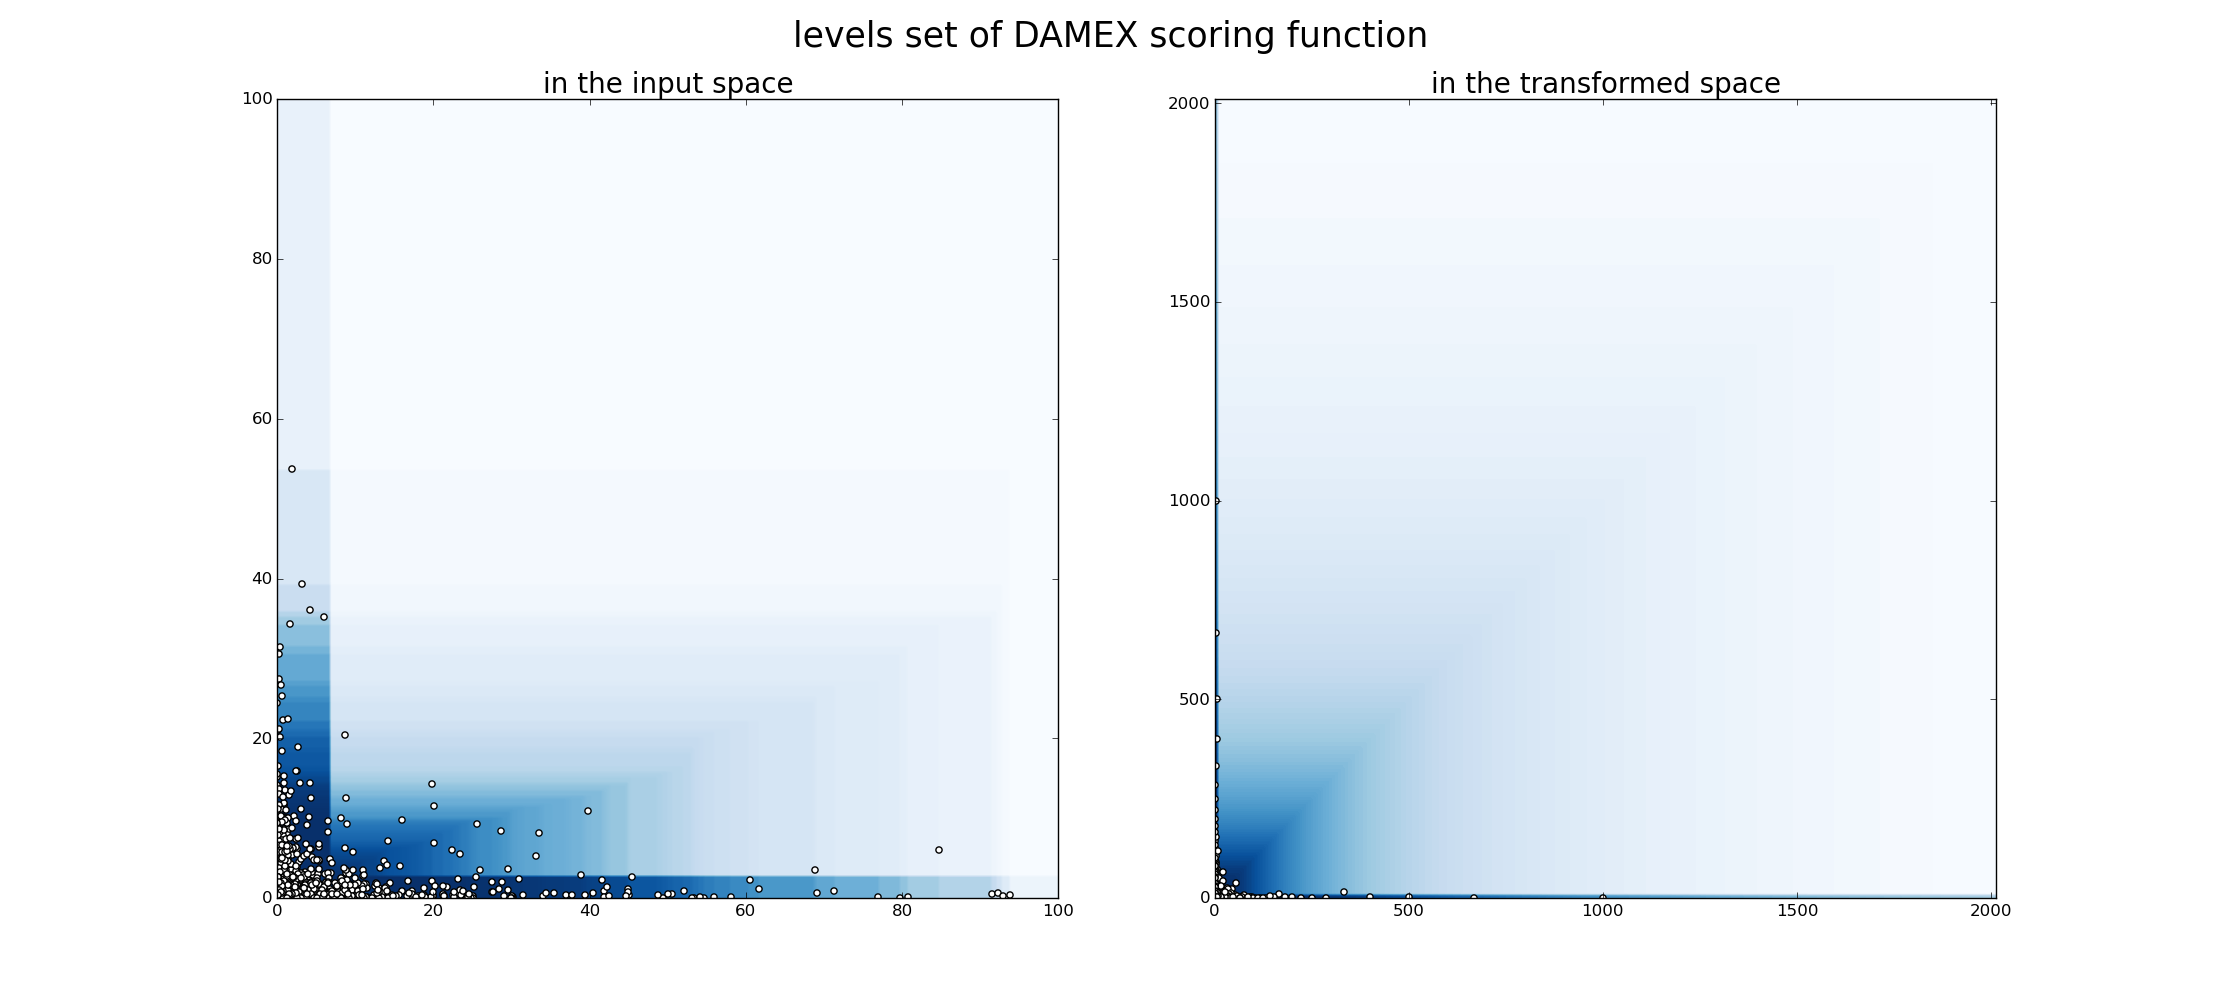
\includegraphics[scale=0.2331]{fig_source/plot_damex_level_sets.png}
\caption{Level sets of $s_n$ on simulated 2D data}
\label{jmva:DAMEX-2D}
\end{figure}

 This heuristic argument explains the following algorithm, referred to as {\it Detecting Anomaly with Multivariate EXtremes}  (DAMEX in abbreviated form). Note that this is a slightly modified version of the original DAMEX algorihtm empirically tested in \cite{AISTAT16}, where $\epsilon$-thickened sub-cones instead of $\epsilon$-thickened rectangles are considered. The proof is more straightforward when considering rectangles and performance remains as good.
The complexity is in $O( dn\log n + dn) = O(dn\log n)$, where the first term on the left-hand-side comes from  computing the $\widehat F_j(X_i^j)$ (Step 1) by sorting  the data (\emph{e.g.} merge sort). The second one arises from Step 2. 

% \begin{center}
% \fbox{
% \begin{minipage}{0.95\linewidth}
\begin{algorithm}[!tbh]
\caption{DAMEX}
\label{jmva:DAMEX-algo}
{\bf Input:} parameters $\epsilon>0$,~~ $k = k(n)$,~~ $p\geq 0$.
\begin{enumerate}
\item Standardize \emph{via} marginal rank-transformation: $\mb{ \widehat V}_i:= \big (1/(1- \widehat F_j (X_i^j))\big)_{j=1,\ldots,d}$~.
\item Assign to each $\mb{\widehat V}_i$ the cone $R_\alpha^\epsilon$
  it belongs to.  
\item Compute $\hatmass(\alpha)$ from (\ref{jmva:heuristic_mu_n2})
   $\rightarrow$ yields: (small number of) cones with non-zero mass.
\item (Optional) Set to $0$ the $\hatmass(\alpha)$ below some small
  threshold defined in remark~\ref{jmva:rk:threshold} \wrt~$p$.%$\mu_{\min}\ge 0$ to eliminate cones with negligible mass
%\\$\rightarrow$ yields: (small number of) cones with non-zero mass
   $\rightarrow$ yields: (sparse) representation of the dependence
  structure 
 \begin{align}
 \label{jmva:phi_n}
\left\{\hatmass(\alpha):\; \emptyset\alpha\subset\{1,\ldots, d\}\right\}.%,~ \hatmass(\alpha)>\mu_{\min}\right\}.
% \Phi_n^\epsilon(v):= \sum_{\alpha} \hatmass(\alpha) \mathds{1}_{v \in \mathcal{C}_\alpha }
 \end{align}
\end{enumerate}
{\bf Output:} Compute the scoring function given
by~(\ref{jmva:def:scoring}), 
\begin{align*}
%\label{jmva:def:scoring}
s_n(\mb x):= (1/\|\widehat T(\mb x)\|_\infty)
\sum_{\alpha }%: \hatmass(\alpha)>\mu_{\min}} 
\hatmass(\alpha) \mathds{1}_{\widehat T(\mb x) \in R_\alpha^\epsilon}.
\end{align*}
\end{algorithm}
% \end{minipage}
% }
% \end{center}

Before investigating how the algorithm above empirically performs when applied to synthetic/real datasets, a few remarks are in order.


\begin{remark}({\sc Interpretation of the Parameters})
\label{jmva:rk_param_interpretation}
In view of %(\ref{jmva:eq:epsilonCone}) and
(\ref{jmva:heuristic_mu_n2}), $n/k$ is the threshold above  which the data are
considered as extreme and $k$ is proportional to the number of such
data, a common approach in multivariate extremes.  % A general
% heuristic in multivariate extreme is that $k$ is proportional to the
% number of data considered as extreme.
The tolerance parameter $\epsilon$ accounts for the  non-asymptotic nature of data. The
smaller $k$, the smaller $\epsilon$ shall be chosen. 
%{\red TODO : $\mu_{\min}$}
The additional angular mass threshold in step 4. acts as an additional
sparsity inducing parameter. Note that even without this additional
step (\ie\ setting $p=0$, the obtained representation for
real-world data (see Table~\ref{jmva:fig:wavedata-nb-faces})  is 
already sparse (the number of charges cones is significantly less than
$2^d$). % For the sake of simplicity, the present paper does not  investigate  the bias induced by $\mu_{\min}$ from a
% theoretical point of view (the main focus here 
% is on the role of $\epsilon$). However, experiments on AD datasets
% show an improved  performance when introducing this additional parameter.  
\end{remark}
\begin{remark}({\sc Choice of Parameters})
\label{jmva:rk_param_choice}
A standard choice of parameters $(\epsilon,~ k ,~ p)$ is
respectively 
$(0.01, n^{1/2}, 0.1)$. % where $\mu_{average}$ is the averaged mass of the non-empty sub-cones, \ie~$\mu_{average}=\mu_{total}/(\#$charged sub-cones)
However, there is no simple manner to choose optimally these parameters, as there is no simple way to determine how fast is the convergence to the (asymptotic) extreme behavior --namely how far in the tail appears the asymptotic dependence structure. Indeed, even though the  first term of the  error bound in Theorem~\ref{jmva:thm-princ} is  proportional, up to re-scaling, to $\sqrt{\frac{1}{\epsilon k} }+ \sqrt{\epsilon}$, which suggests choosing $\epsilon$ of order $ k^{-1/4}$, the unknown bias term perturbs the analysis and in practice, one obtains better results with the values above mentioned. 
In a supervised or novelty-detection framework (or if a small labeled dataset is available) these three parameters should be chosen by cross-validation.
In the unsupervised situation, a classical heuristic
(\cite{Coles2001}) is to choose $(k, \epsilon)$ in a stability region
of the algorithm's output: the largest $k$ (\emph{resp.} the larger
$\epsilon$) such that when decreased, the dependence structure remains
stable. This amounts to selecting as many  data as possible as being
extreme (\emph{resp. } in  low dimensional regions), within a stability
domain of the estimates, which exists under the primal assumption
\eqref{jmva:intro:assumption2} and in view of Lemma~\ref{jmva:lem:limit_muCalphaEps}. %constrained to observing the stability induced by the asymptotic behavior.
\end{remark}
\begin{remark} ({\sc Dimension Reduction})
If the extreme dependence structure is low dimensional, namely
concentrated on low dimensional cones $\mathcal{C}_\alpha$ -- or in other terms if only a
limited number of margins can be large together -- then most of the
$\widehat V_i$'s will be concentrated on the $R_\alpha^\epsilon$'s
such that  $|\alpha|$ (the dimension of the cone $\mathcal{C}_\alpha$)
is small; then the
representation of the dependence structure
% representation $\phi_n^\epsilon$
 in (\ref{jmva:phi_n}) is both sparse and low dimensional.
\end{remark}

\begin{remark} ({\sc Scaling Invariance})
DAMEX produces the same result if the input data are transformed in such a way that the marginal order is preserved. In particular, any marginally increasing transform or any scaling as a preprocessing step does not affect the algorithm. It also implies invariance with respect to any change in the measuring units. This invariance property constitutes part of the strengh of the algorithm, since 
data preprocessing steps usually have a great impact on the overall performance and are of major concern in pratice.
%looking for the best way to preprocess the data has a great influence on the performance and is a major concern in practice.
\end{remark}
% The next section provides a theoretical ground for Algorithm~\ref{jmva:DAMEX-algo}. 
% As shall be shown below, it  amounts to
% learning  the dependence structure of extremes (in particular, its support).
% The dependence parameter $\hatmass(\alpha)$ 
% % scoring function (\ref{jmva:def:scoring})
% actually coincides with a
% (voluntarily $\epsilon$-biased) natural estimator of $\mu(\mathcal{C}_\alpha)$, where $\mu$
% is  a `true' measure of the extremal dependence,
% namely the exponent measure defined as $\lim_{n \to \infty}
% \frac{n}{k} \mathbb{P} \left[V \in \frac{n}{k}~ (\point) \right] $.
% Section~\ref{jmva:sec:estimation} develops uniform, non-asymptotic upper
% bounds on  the error 
% $|\hatmass(\alpha) - \mu(\mathcal{C}_\alpha)|$ to attest the theoretical quality of this estimate.
% Providing empirical result on simulated and real data.
% The two following sections are to prove an inequality (Theorem \ref{jmva:thm-princ}) of type 
% \begin{align*}
% |\mu_n(\mathcal{C}_\alpha^\epsilon) - \mu(\mathcal{C}_\alpha)| ~\le~ \left( \frac{C \sqrt d}{k^{1/4}} \sqrt{ \log\frac{d}{\delta}} ~+~ b(n) \right)
% \end{align*}
% with $b(n)$ the model biais, $\mu_n(\mathcal{C}_\alpha^\epsilon) = \hatmass(\alpha)$, and $\mu$ the `true measure of the extreme behavior' namely the exponent measure defined as $\lim_{n \to \infty} \frac{n}{k} \mathbb{P} \left[V_1 \in \frac{n}{k}~. \right] $ in the sense of the weak convergence, where $V_i:= \left ( \frac{1}{1- F_j (X_i^l)}\right)_{l=1..d}$.

%%% Local Variables: 
%%% mode: latex
%%% TeX-master: t
%%% End: 

\section{Experimental results}
\label{jmva:sec:experiments}
%\subsection{Sparse dependence structure of real data}
\subsection{Recovering the support of the dependence structure of generated data}
Datasets of size $50000$ (respectively $100000$, $150000$) are  generated in $\mathbb{R}^{10}$ according to a popular multivariate extreme value
model, introduced by \cite{Tawn90},  namely a multivariate asymmetric
logistic distribution ($G_{log}$). %  one
% model ,
The data have the following features: (i) they resemble `real life'
data, that is, the $X_i^j$'s are non
zero  and the transformed $\hat V_i$'s belong to the interior cone
$\mathcal{C}_{\{1,\ldots,d\}}$, (ii) the associated (asymptotic) exponent measure concentrates on
 $K$ disjoint cones $\{\mathcal{C}_{\alpha_m} , 1\le m\le K\}$.  % where the
 % $D = \{\alpha_m , 1\le m\le k\}$ is a partition of $\{1,\ldots d\}$  (the latter requirement simplifies the
 % model's specification). Note that, in this context, the number of
 % `non-zero' faces is $K\le d$.
 For the sake of reproducibility, % we give the
 % expression for the \emph{c.d.f.} $G$ from which the data is
 % drawn,  % Here, $D = \{\alpha_1,\ldots\alpha_k\}$ denote the disjoint
 % % subsets of indices such that $\mu(\mathcal{C}_{\alpha_m})\neq 0$,
 % % $m\le k$.
 $$ G_{log}(\mb x) = \exp\{ - \sum_{m = 1}^K \left(\sum_{j \in \alpha_m}
     (|A(j)|x_j)^{ - 1/{w_{\alpha_m}}}\right)^{w_{\alpha_m}} \}, $$
 where $|A(j)|$ is the cardinal of the set $\{\alpha\in D: j \in
 \alpha\}$ and where $w_{\alpha_m} = 0.1$ is a dependence parameter
 (strong dependence). %  in
 % $(0,1]$ that we set to $0.1$ : the dependence on
 % $\mathcal{C}_{\alpha_m}$ is a decreasing function of
 % $w_{\alpha_m}$.
 % For our simulations, $w_{\alpha_m}$ is set to $0.1$.
% We simulate 50000 observations of a multivariate asymmetric logistic
% model in $\mathbb{R}^{10}$, introduced by \cite{Tawn90}. 
%  and whose exponent measure is $\mu([0, \mb x]^c) = -\log(G_0(\mb x))$ with 
% \begin{align*}
% G_0(x) = \sum_{\alpha \in A} \left(\sum_{i \in \alpha} \left(\frac{\theta_{i,\alpha}}{x_i} \right)^{1/w_\alpha}\right)^{w_\alpha} .
% \end{align*}
% Here $A$ is the set of all non-empty subsets of $\dd$,
% $\theta_{i,\alpha} = 0$ for all $\alpha \notin D$, $D \dd \setminus \emptyset $ is a subset of faces,
% and $\theta_{i,\alpha} = \frac{1}{|A_{(i)}|}$ with $|A_{(i)}|$ is the cardinal of the set $A_{(i)} = \{\alpha \in A, i \in \alpha\}$. Note that for each subset of features $\alpha$, either the $\theta_{i,\alpha}$ are all null, either they are all positive. We choose $w_\alpha$ to be $1$ for every $\alpha$, since we want a maximal asymptotic dependence between the chosen subsets of features (namely the $\alpha$ such that $\forall i,~\theta_{i,\alpha} \neq 0$). This simulation thus consider only two cases for each subset of features $\alpha$: either they are dependent and there is a non-negligeable asymptotic mass on the corresponding face (charged by $\mu$); either they are independent and have thus no mass asymptotically ($\mu$ has no mass on such faces).
The data are simulated using  Algorithm 2.2 in \cite{Stephenson2003}.
The subset of sub-cones $D$ charged by $\mu$ is randomly chosen (for each
fixed number of sub-cones $K$) and the purpose is to recover $D$ by Algorithm~\ref{jmva:DAMEX-algo}.
  For each $K$, $100$ experiments
are made and we consider  the  number of `errors', that is,      the number of
non-recovered or false-discovered sub-cones. Table~\ref{jmva:table:logevd} shows the averaged
numbers of errors  among the $100$ experiments. %% (multiplied by $100$ for
%%readability). 
\begin{table}[!ht]
\caption{Support recovering on simulated data}
\label{jmva:table:logevd}
\centering
\resizebox{\linewidth}{!} {
\begin{tabular}{c ccccccccccc}
  \toprule
  $\#$ sub-cones $K$       &    3 & 5    &  10   & 15   & 20    & 25  & 30   & 35    & 40    & 45    & 50 \\
  \midrule
 Aver. $\#$ errors ~~(n=5e4)     & 0.02 & 0.65 & 0.95  & 0.45 & 0.49  & 1.35& 4.19 & 8.9  & 15.46  & 19.92  & 18.99 \\
   %(n=5e4)     &&&&&&&&&&& \\

 Aver. $\#$ errors (n=10e4)    & 0.00 & 0.45 & 0.36  & 0.21 & 0.13  & 0.43& 0.38 & 0.55  & 1.91  & 1.67  & 2.37 \\
%   (n=10e4)     &&&&&&&&&&& \\

 
 Aver. $\#$ errors (n=15e4)    & 0.00  & 0.34 & 0.47 & 0.00 & 0.02  & 0.13& 0.13 & 0.31  & 0.39  & 0.59  & 1.77 \\
%(n=15e4) &&&&&&&&&&& \\
 % Aver. $\#$ errors (n=15e4)    & 0.01 & 0.01 & 0.06  & 0.02 & 0.39  & 1.12& 1.82 & 3.59  & 6.59  & 8.06  & 11.21 \\fi
 %  \hline
  \bottomrule
\end{tabular}
}
\end{table}
The results are very promising in situations where the number of sub-cones is moderate \emph{w.r.t.} the number of observations. %  Also, additional experiments (not shown here) indicate

\subsection{Sparse structure of extremes  (wave data)}
Our goal is here to verify that the two expected phenomena mentioned
in the introduction, \textbf{1-}~sparse dependence structure of extremes (small number
of sub-cones with non zero mass), \textbf{2-}~low dimension of the
sub-cones with non-zero mass,  do occur with real data. 
%We test the sparsity in the extreme dependence structure of 
We consider wave
directions data provided by Shell, which consist of $58585$
measurements  $D_i$, $i\le 58595$ of wave directions between $0^{\circ}$ and $360^{\circ}$ at $50$ different
locations (buoys in North sea). The dimension is thus $50$. % , each sample
% representing a different record time.
The angle $90^{\circ}$ being fairly
rare, we work with data obtained as $X_i^j = 1/(10^{-10} + |90-
D_i^j|)$, where $D_i^j$ is the wave direction at buoy $j$, time $i$. Thus,
$D_i^j$'s close to $90$ correspond to  extreme $X_i^j$'s.
% we chose to apply the transform $1/(1e^{-10} + \|90-.\|)$ to the
% data in order to make it
% extreme. % extremes the $90$ degree observations
Results in
% Figure~\ref{jmva:fig:wavedata-dim}~and
Table~\ref{jmva:fig:wavedata-nb-faces}% ($\mu_{total}$ denotes the total probability mass of $\mu$)
show that 
the %dimensions 
number of  sub-cones $\mathcal{C}_\alpha$ identified by Algorithm~\ref{jmva:DAMEX-algo}
is indeed small compared to the total number of sub-cones ($2^{50}$-1).
% supporting the  extreme data  
%%are  essentially lower than $15$
(Phenomenon \textbf{1} in the introduction section). 
Further, the dimension of these sub-cones is essentially moderate
(Phenomenon \textbf{2}):
respectively $93\%$, $98.6\%$ and  $99.6\%$
of the mass is affected to  sub-cones of dimension no greater  than $10$,
$15$ and $20$ respectively %  ???????????,
% with a maximal dimension of ?????????? 
(to be compared with $d=50$).  Histograms displaying the mass repartition produced by Algorithm~\ref{jmva:DAMEX-algo} are given in Fig.~\ref{jmva:fig:wavedata-dim}.
% and
% their  number is %of such faces charged by the exponent measure $\mu$ is
% small (phenomenon \textbf{1}) compared to the total number of sub-cones ($2^{50}$-1).
\begin{figure}[!ht]
\centering
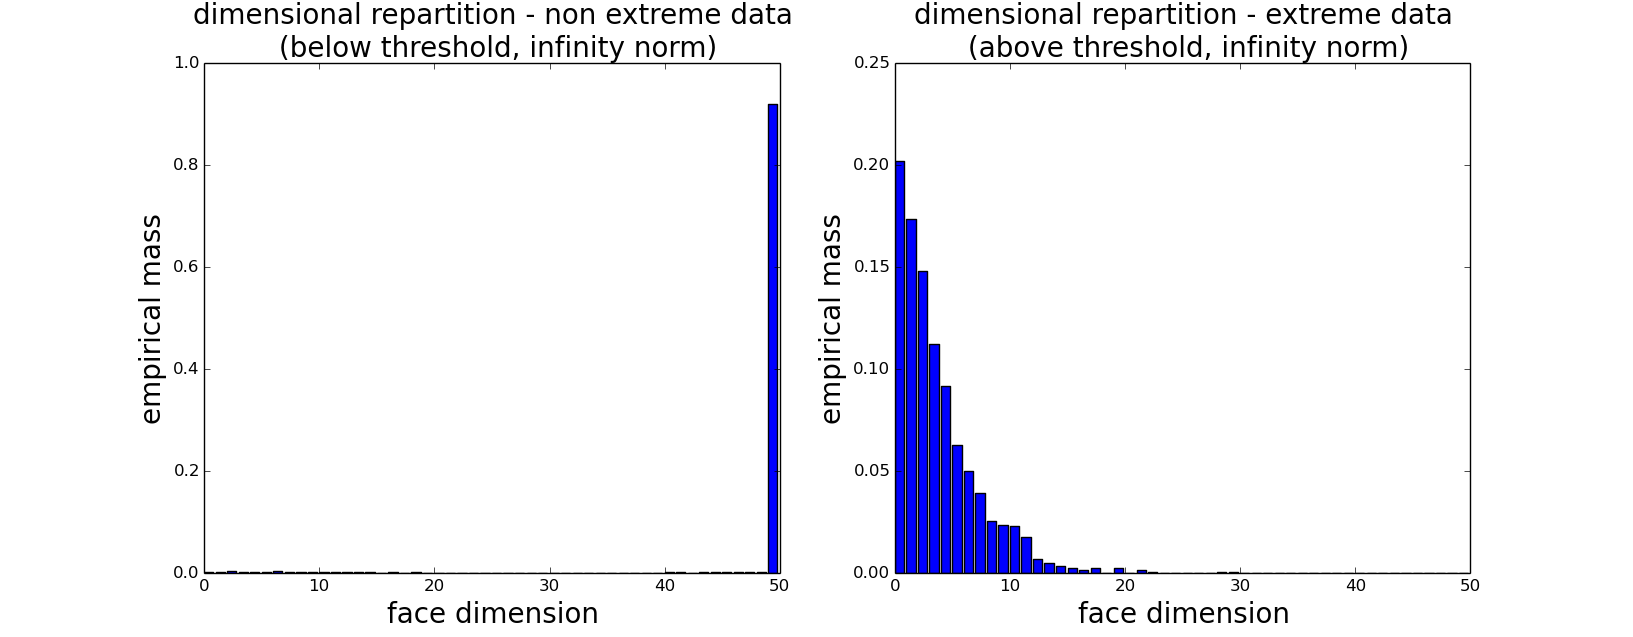
\includegraphics[scale=0.33]{fig_source/wave_dir2}
\caption{sub-cone dimensions of wave data}
\label{jmva:fig:wavedata-dim}
\end{figure}

\begin{table}[!ht]
\caption{Total number of sub-cones of wave data}
\label{jmva:fig:wavedata-nb-faces}
\centering
%\resizebox{\linewidth}{!} {
\begin{tabular}{lcc}
\toprule
~ & non-extreme data & extreme data \\
\midrule
nb of sub-cones with mass $>0$ ($p = 0$) & 3413 & 858 \\
idem after thresholding ($p = 0.1$) & 2 & 64 \\
idem after thresholding ($p = 0.2$) & 1 & 18 \\ 
\bottomrule
\end{tabular}
%}
\end{table}


\subsection{Application to Anomaly Detection on real-world data sets}

% \noindent
% \begin{minipage}{0.5\linewidth}
% \centering
% \includegraphics[scale=0.17]{fig_source/extreme_AD}
% \captionof{figure}{\tiny Combination of any standard AD algorithm with DBAD}
% \label{jmva:fig:combination}
% \end{minipage}\hfill
% \begin{minipage}{0.5\linewidth}
% \end{minipage}
%We point out that
 The main purpose of Algorithm~\ref{jmva:DAMEX-algo} is to build a 
 `normal profile' for 
extreme data, so as to distinguish between normal and ab-normal
extremes. 
In this section we evaluate its performance %on such region
 and compare it with that of a standard anomaly detection algorithm, %  that it may be combined with a
% standard AD algorithm  to handle extreme \emph{and} non-extreme data,
% improving the global performance of the chosen standard algorithm.
% In this section we show that it may be combined with a
% standard AD algorithm  to handle extreme \emph{and} non-extreme data,
% improving the global performance of the chosen standard algorithm.
% which focusing on non-extreme data. 
% This can be done as
% illustrated in Fig.~\ref{jmva:fig:combination} by splitting the input
% space between an extreme region and a non-extreme one, then applying
% Algorithm~\ref{jmva:DAMEX-algo} to the extreme region, while the
% non-extreme one is processed with the standard
% algorithm.
the Isolation Forest (iForest)
algorithm, which we chose in view of its
established high performance (\cite{Liu2008}). 
The two algorithms are trained and tested on the same datasets, the
test set being restricted to an  extreme region.
% Our aim is to compare the results obtained with the
% combined method
%  `iForest + DAMEX' above described, to those obtained with iForest
%  alone on the whole input space. 
% A random forest AD algorithm is chosen as an exemplary `standard' one,
% namely the Isolation Forest (iForest) algorithm (in view of its high performances)
% . We compare its own use, with when combined with Algorithm~\ref{jmva:DAMEX-algo} as illustrated in Figure~\ref{jmva:fig:combination}.
 Five reference anomaly detection datasets  are considered:
 \emph{shuttle}, \emph{forestcover}, \emph{http},
 \emph{SF} and \emph{SA} \footnote{These datasets are available for instance on http://scikit-learn.org/dev/ }. The experiments are performed in a
 novelty detection framework (the training set consists of normal data). 
% In a  non-supervised framework (training set including abnormal data), the
%  improvements brought by the use of DAMEX are less significant, but the
%  precision score is still increased % on five datasets out of six, 
%  when the recall is high (high rate of true positives), inducing more vertical ROC curves near the origin.
%
 % When done on both normal and abnormal data, the results are less impressive but there is still an improvement of the precision on five of the six datasets when the recall is high (namely when the true positive rate is large).
%

The \emph{shuttle} dataset is the fusion of the training and testing datasets
available in the UCI repository \cite{Lichman2013}. The data have $9$
 numerical attributes,  the first one being time. Labels from $7$ different classes are also
 available. Class $1$ instances are considered as normal, the others as anomalies. 
We use instances from all different classes but class $4$,  % classes $1, 2,3,5,6$ and $7$ (class In our experiments, the class $1$ is considered as normal and instances from class $2, 3, 5, 6, 7$ are anomalies,
which yields an anomaly ratio (class 1) of $7.17\%$. %
%Instances from class $4$ are not used.
%

In the \emph{forestcover} data, also available at UCI
repository (\cite{Lichman2013}), the normal data are the  instances
from class~$2$ while instances from class $4$ are anomalies, other classes are omitted, 
so that the  anomaly ratio for this dataset is  $0.9\%$. 
%

The last three datasets belong to the KDD Cup '99 dataset
(\cite{KDD99}, \cite{Tavallaee2009}), produced by processing the
tcpdump portions of the 1998 DARPA Intrusion Detection System (IDS)
Evaluation dataset, created by MIT Lincoln Lab \cite{Lippmann2000}.
The artificial data was generated using a closed network and a wide
variety of hand-injected attacks (anomalies) to produce a large number
of different types of attack with normal activity in the background.
Since the original demonstrative purpose of the dataset concerns
supervised anomaly detection, the anomaly rate is very high ($80\%$), which is
unrealistic in practice, and inappropriate for evaluating the
performance on realistic data.  We thus take standard pre-processing
steps in order to work with smaller anomaly rates. For datasets
\emph{SF} and \emph{http} we proceed as described in
\cite{Yamanishi2000}: \emph{SF} is obtained by picking up the data
with positive logged-in attribute,
and %using only four attributes thus
focusing on the intrusion attack, which gives an anomaly proportion of
$0.48\%.$ %$0.3\%$.
The dataset \emph{http} is a subset of \emph{SF} corresponding to a
third feature equal to 'http'.
%
Finally, the \emph{SA} dataset  is obtained as in \cite{Eskin2002} by 
selecting all the normal data, together with a small proportion
($1\%$) of anomalies. % abnormal data  % to gives an anomaly proportion of $1\%$.
% Moreover, the 3 categorical
% attributes have been binary encoded.
%

Table~\ref{jmva:table:data} summarizes the characteristics of these
datasets. 
The thresholding parameter $p$ is fixed to $0.1$, the averaged mass of the non-empty sub-cones, while the parameters $(k,\epsilon)$ are standardly chosen as $(n^{1/2}, 0.01)$.
The extreme region on which the evaluation step is performed is chosen
as $\{\mb x:~ \|T(\mb x)\| > \sqrt{n} \}$, where $n$ is the  training
set's sample size. The ROC and PR curves are computed using only observations in the extreme region. This provides a precise evaluation of the two anomaly detection methods on extreme data.
 % As the datasets \emph{http}, \emph{smtp} and \emph{SF} do not have enough features to consider the stability, we choose the (standard) parameters $(k, \epsilon) = (n^{1/2}, 0.01)$. 
For each of them, 20 experiments on random training and testing datasets are performed, yielding averaged ROC and Precision-Recall curves whose AUC are presented in Table~\ref{jmva:table:results-dbad+iforest-01}.
%
DAMEX significantly improves the performance (both in term of precision and of ROC curves) in extreme regions
for each dataset, as illustrated in figures \ref{jmva:fig:shuttle} and \ref{jmva:fig:SF}.

In Table~\ref{jmva:table:results-dbad+iforest-1}, we repeat the same experiments but with $\epsilon=0.1$.
This yields the same strong performance of DAMEX, excepting for \emph{SF} (see Figure~\ref{jmva:fig:SF_1}).
Generally, to large $\epsilon$ may yield over-estimated
$\hatmass(\alpha)$ for low-dimensional faces $\alpha$.
Such a performance gap between $\epsilon=0.01$ and $\epsilon=0.1$ can also be explained by the fact that anomalies may form a cluster which is wrongly include in some over-estimated `normal' sub-cone, when $\epsilon$ is too large. Such singular anomaly structure would also explain the counter performance of iForest on this dataset.

% on this dataset with $\epsilon=0.1$, DAMEX has lower performance than iForest. Its ROC
% curve has a slow slope at the origin (Fig.~\ref{jmva:fig:SF}), which reflects a lack of
% precision when assigning high abnormal scores. This may be explained
% by the fact that % anomalies belong to some low dimensional faces for which
% the estimate
% $\hatmass(\alpha)$ is too biased (over-estimated) for low-dimensional faces $\alpha$, using a too large tolerance parameter $\epsilon$, and can even wrongly include anomalies which were in the central cone, despite quite close to the border.

% , or by the simple fact that the asymptotic dependence
% structure has not quite been reached at this level $k = n^{1/2}$.
%on this dataset, the algorithm seems unable to capture any extreme
%dependence structure, either because the latter is non-existent (no
%regularly varying tail), either because the convergence is too slow
%to appear in our relatively small dataset.
%
% Smaller values of $\epsilon$ reduce the bias and Fig.~\ref{jmva:fig:SF-01}
% shows that decreasing $\epsilon$ clearly improves the performance
% on regions where the abnormality score is large (near the origin on
% the ROC and Precision/Recall plots). 

We also point out that for very small values of epsilon ($\epsilon \le 0.001$),
the performance of DAMEX significantly decreases on these datasets.
With such a small $\epsilon$, most observations belong to the central cone
(the one of dimension $d$) which is widely over-estimated, while the other cones are under-estimated.%  and no discrimination measure
% appears except the norm of the observations.

The only case were using very small $\epsilon$ should be useful, is when the asymptotic behaviour is
clearly reached at level $k$ (usually for very large threshold $n/k$, \eg~$k=n^{1/3}$), or in the
specific case where anomalies clearly concentrate in low dimensional sub-cones: The use of a small $\epsilon$ precisely allows
to assign a high abnormality score to these subcones (under-estimation of the asymptotic mass), which yields better performances.

% While Fig.~\ref{jmva:fig:SF} displays the ROC and
% PR curves for the standard parameter $\epsilon = 0.1$,
% Fig.~\ref{jmva:fig:SF-01} shows the same
% curves obtained with $\epsilon=0.01$. For
% this dataset, decreasing $\epsilon$ clearly improves the performance
% on regions where the abnormality score is large (near the origin on
% the ROC and Precision/Recall plots). 

% With
% such a small $\epsilon$, more observations belong to the central cone
% (the one of dimension $d$). It is then difficult to detect anomalies
% in this cone if their radius are not larger than the normal
% observations. However, if the anomalies are concentrated in smaller
% dimensional subcones, those subcones are possibly over-estimated using
% too large $\epsilon$. The use of a smaller $\epsilon$ precisely allows
% to assign a high abnormality score to these subcones, which yields
% better performances.
The averaged ROC curves and PR curves for the other datasets are represented in Figures
\begin{table}[!ht]
\caption{Datasets characteristics}
\label{jmva:table:data}
\centering
%\footnotesize
\begin{tabular}{lccccc}
  \toprule
   ~                   & shuttle & forestcover & SA     & SF     & http    \\
  \midrule
  Samples total        & 85849   & 286048      & 976158 & 699691 & 619052  \\
  Number of features   & 9       & 54          & 41     & 4      & 3       \\
  Percentage of anomalies & 7.17    & 0.96        & 0.35   & 0.48   & 0.39 \\
\bottomrule
\end{tabular}
\end{table}

%TODO: rappel PR et ROC
\begin{table}[!ht]
\caption{Results on extreme regions with standard parameters $(k,\epsilon) = (n^{1/2}, 0.01)$}
\label{jmva:table:results-dbad+iforest-01}
\centering
\begin{tabular}{lcccc}
  \toprule
Dataset      &\multicolumn{2}{c}{iForest}& \multicolumn{2}{c}{DAMEX}\\\hline
~            &AUC ROC       & AUC PR     &AUC ROC     &AUC PR       \\
shuttle      & 0.957        & 0.987      &$\mb{0.988}$&$\mb{0.996}$ \\
forestcover  & 0.667        & 0.201      &$\mb{0.976}$&$\mb{0.805}$ \\
http         & 0.561        & 0.321      &$\mb{0.981}$&$\mb{0.742}$ \\
%smtp         & $\mb{0.900}$ &$\mb{0.004}$&0.898       &0.003        \\
SF           & 0.134        & 0.189      &$\mb{0.988}$&$\mb{0.973}$ \\
SA           & 0.932        &0.625       &$\mb{0.945}$&$\mb{0.818}$ \\ 
\bottomrule
\end{tabular}
\end{table}


\begin{table}[!ht]
\caption{Results on extreme regions with lower $\epsilon=0.1$}
\label{jmva:table:results-dbad+iforest-1}
\centering
\begin{tabular}{lcccc}
  \toprule
Dataset      &\multicolumn{2}{c}{iForest}& \multicolumn{2}{c}{DAMEX}\\\hline
~            &AUC ROC       & AUC PR     &AUC ROC     &AUC PR       \\
shuttle      & 0.957        & 0.987      &$\mb{0.980}$&$\mb{0.995}$ \\
forestcover  & 0.667        & 0.201      &$\mb{0.984}$&$\mb{0.852}$ \\
http         & 0.561        & 0.321      &$\mb{0.971}$&$\mb{0.639}$ \\
%smtp         & $\mb{0.900}$ &$\mb{0.004}$&0.898       &0.003        \\
SF           & $\mb{0.134}$ & 0.189      &0.101       &$\mb{0.211}$ \\
SA           & 0.932        &0.625       &$\mb{0.964}$&$\mb{0.848}$ \\ 
\bottomrule
\end{tabular}
\end{table}


\begin{figure}[!ht]
  \centering
  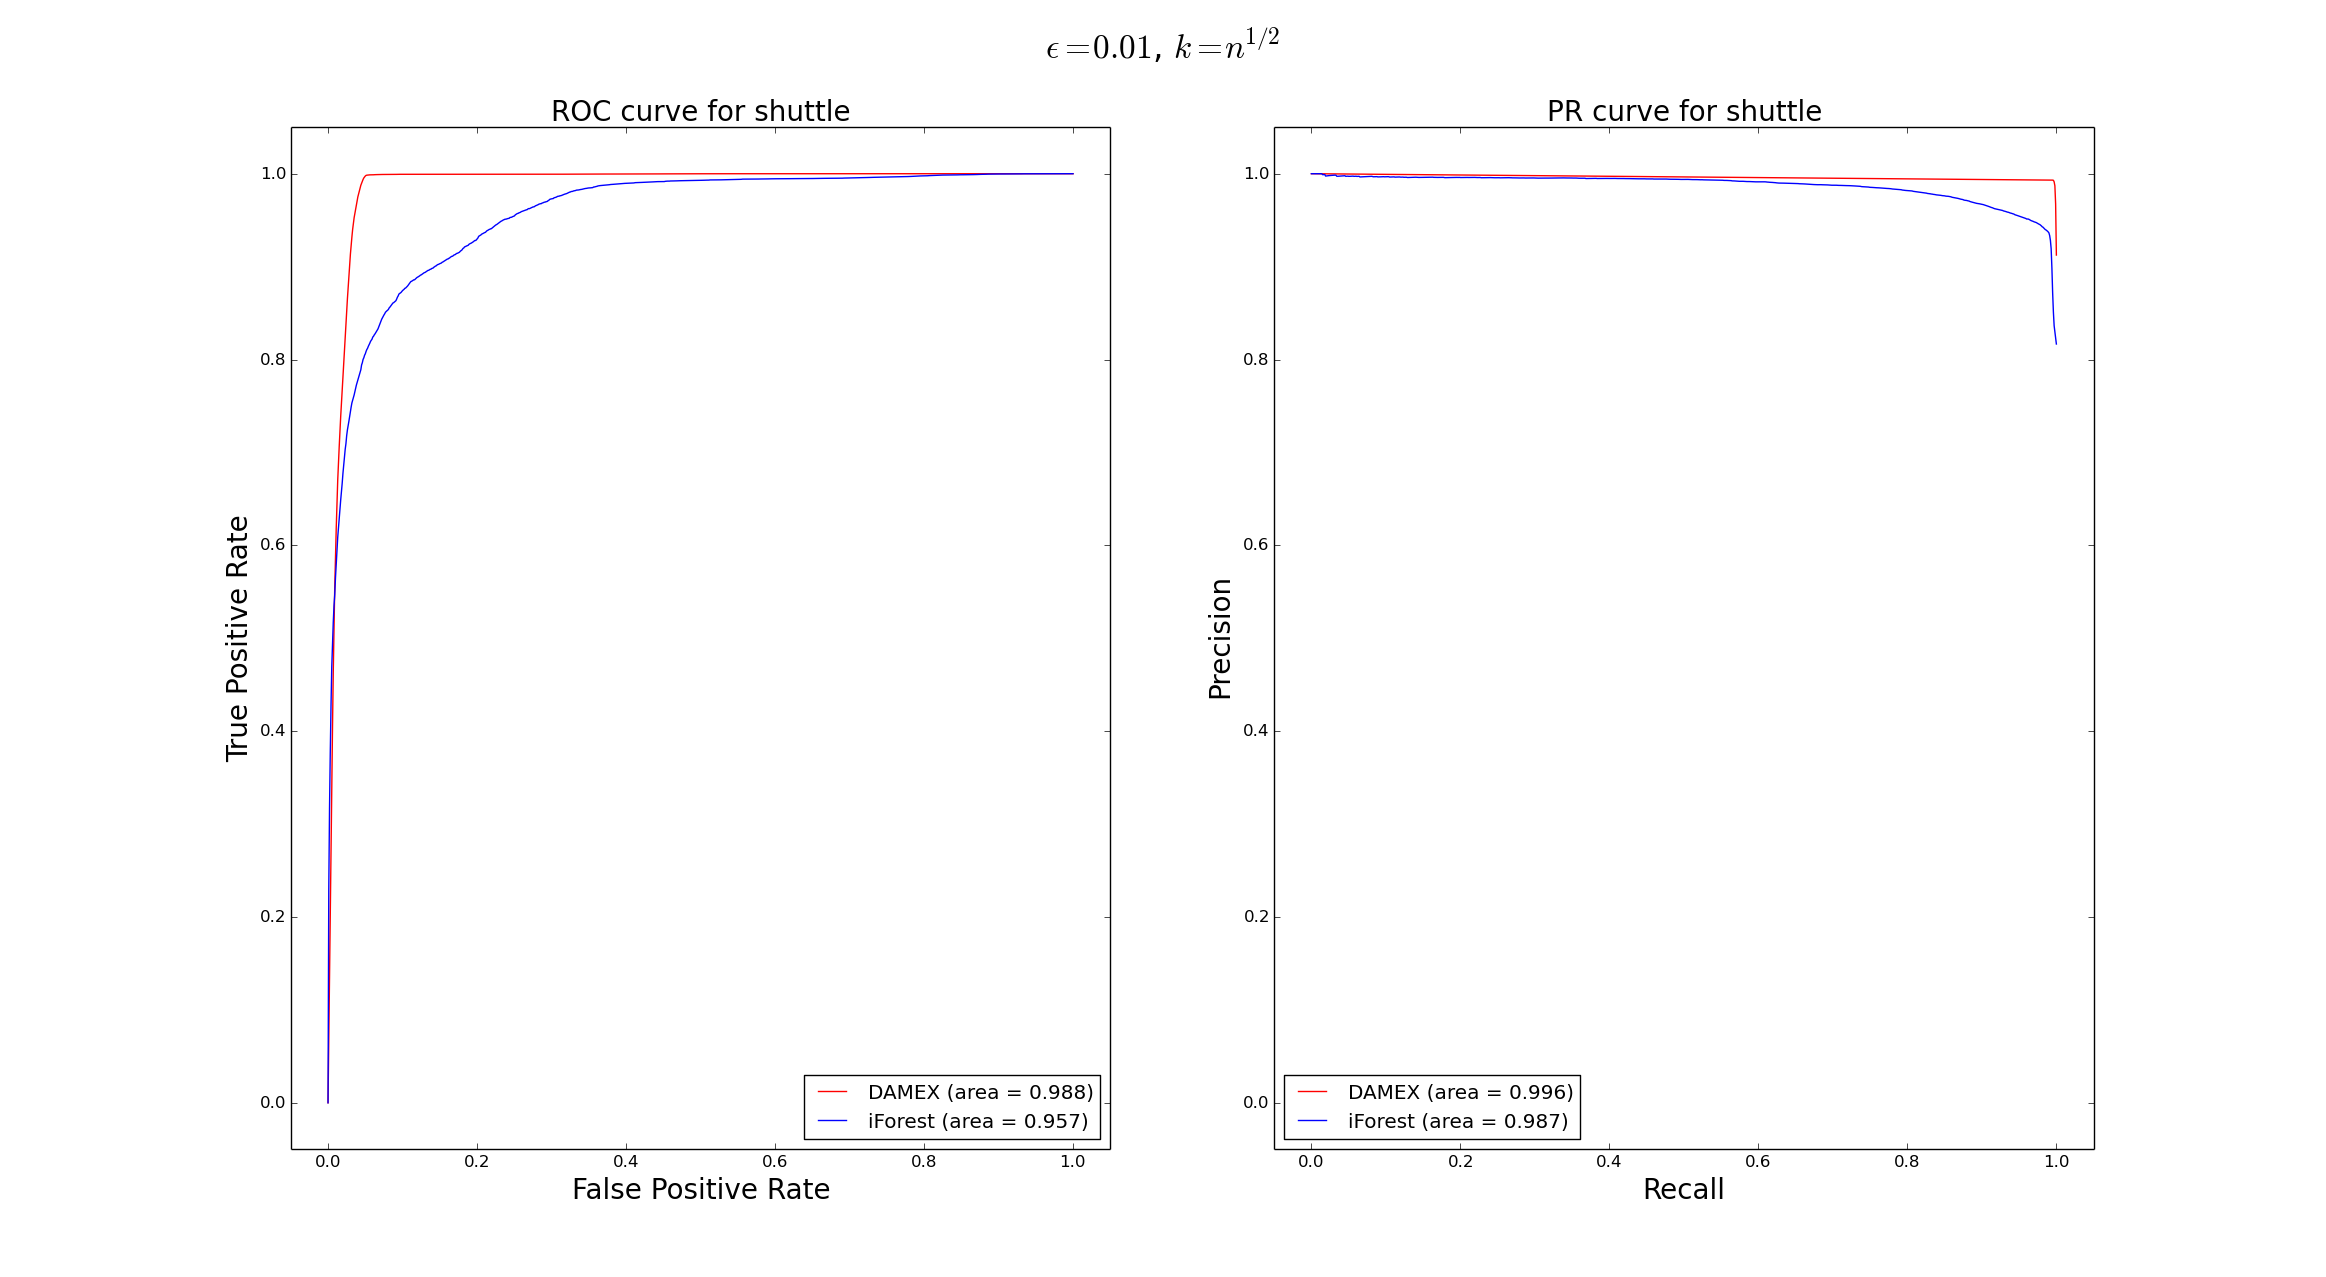
\includegraphics[width = \textwidth]{fig_source/shuttle-semi-supervised-average-rect-01.png}
  \caption{SF dataset, default parameters}
\label{jmva:fig:shuttle}
\end{figure}
\begin{figure}[!ht]
  \centering
  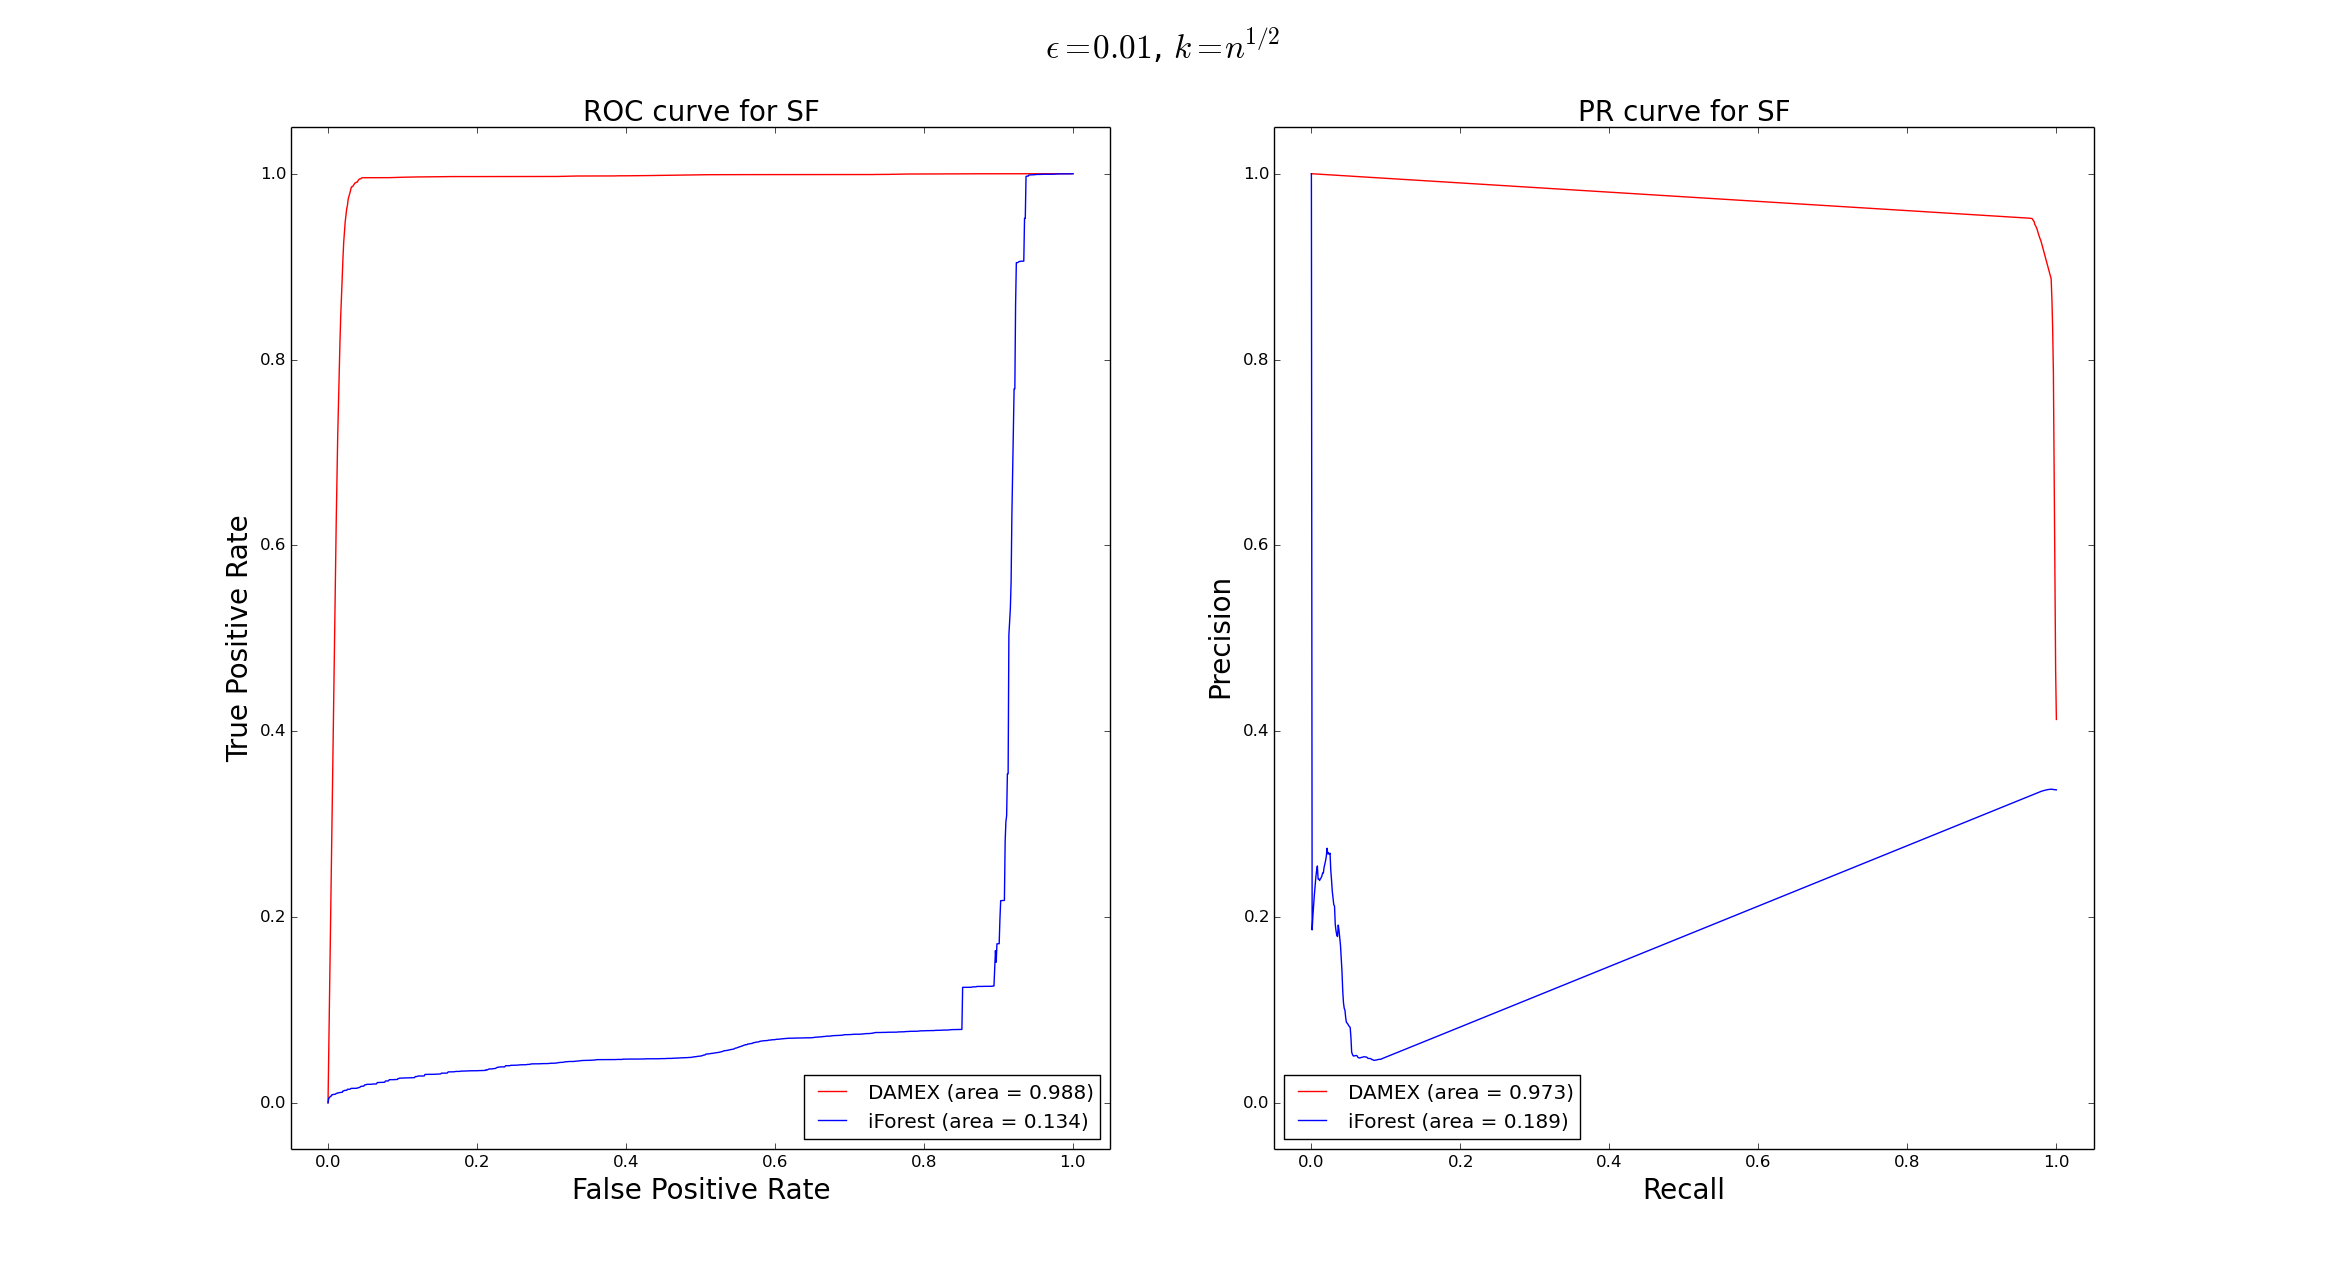
\includegraphics[width = \textwidth]{fig_source/SF-4d-lb-semi-supervised-average-rect-01}
  \caption{SF dataset, larger $\epsilon$}
\label{jmva:fig:SF}
\end{figure}
\begin{figure}[!ht]
  \centering
  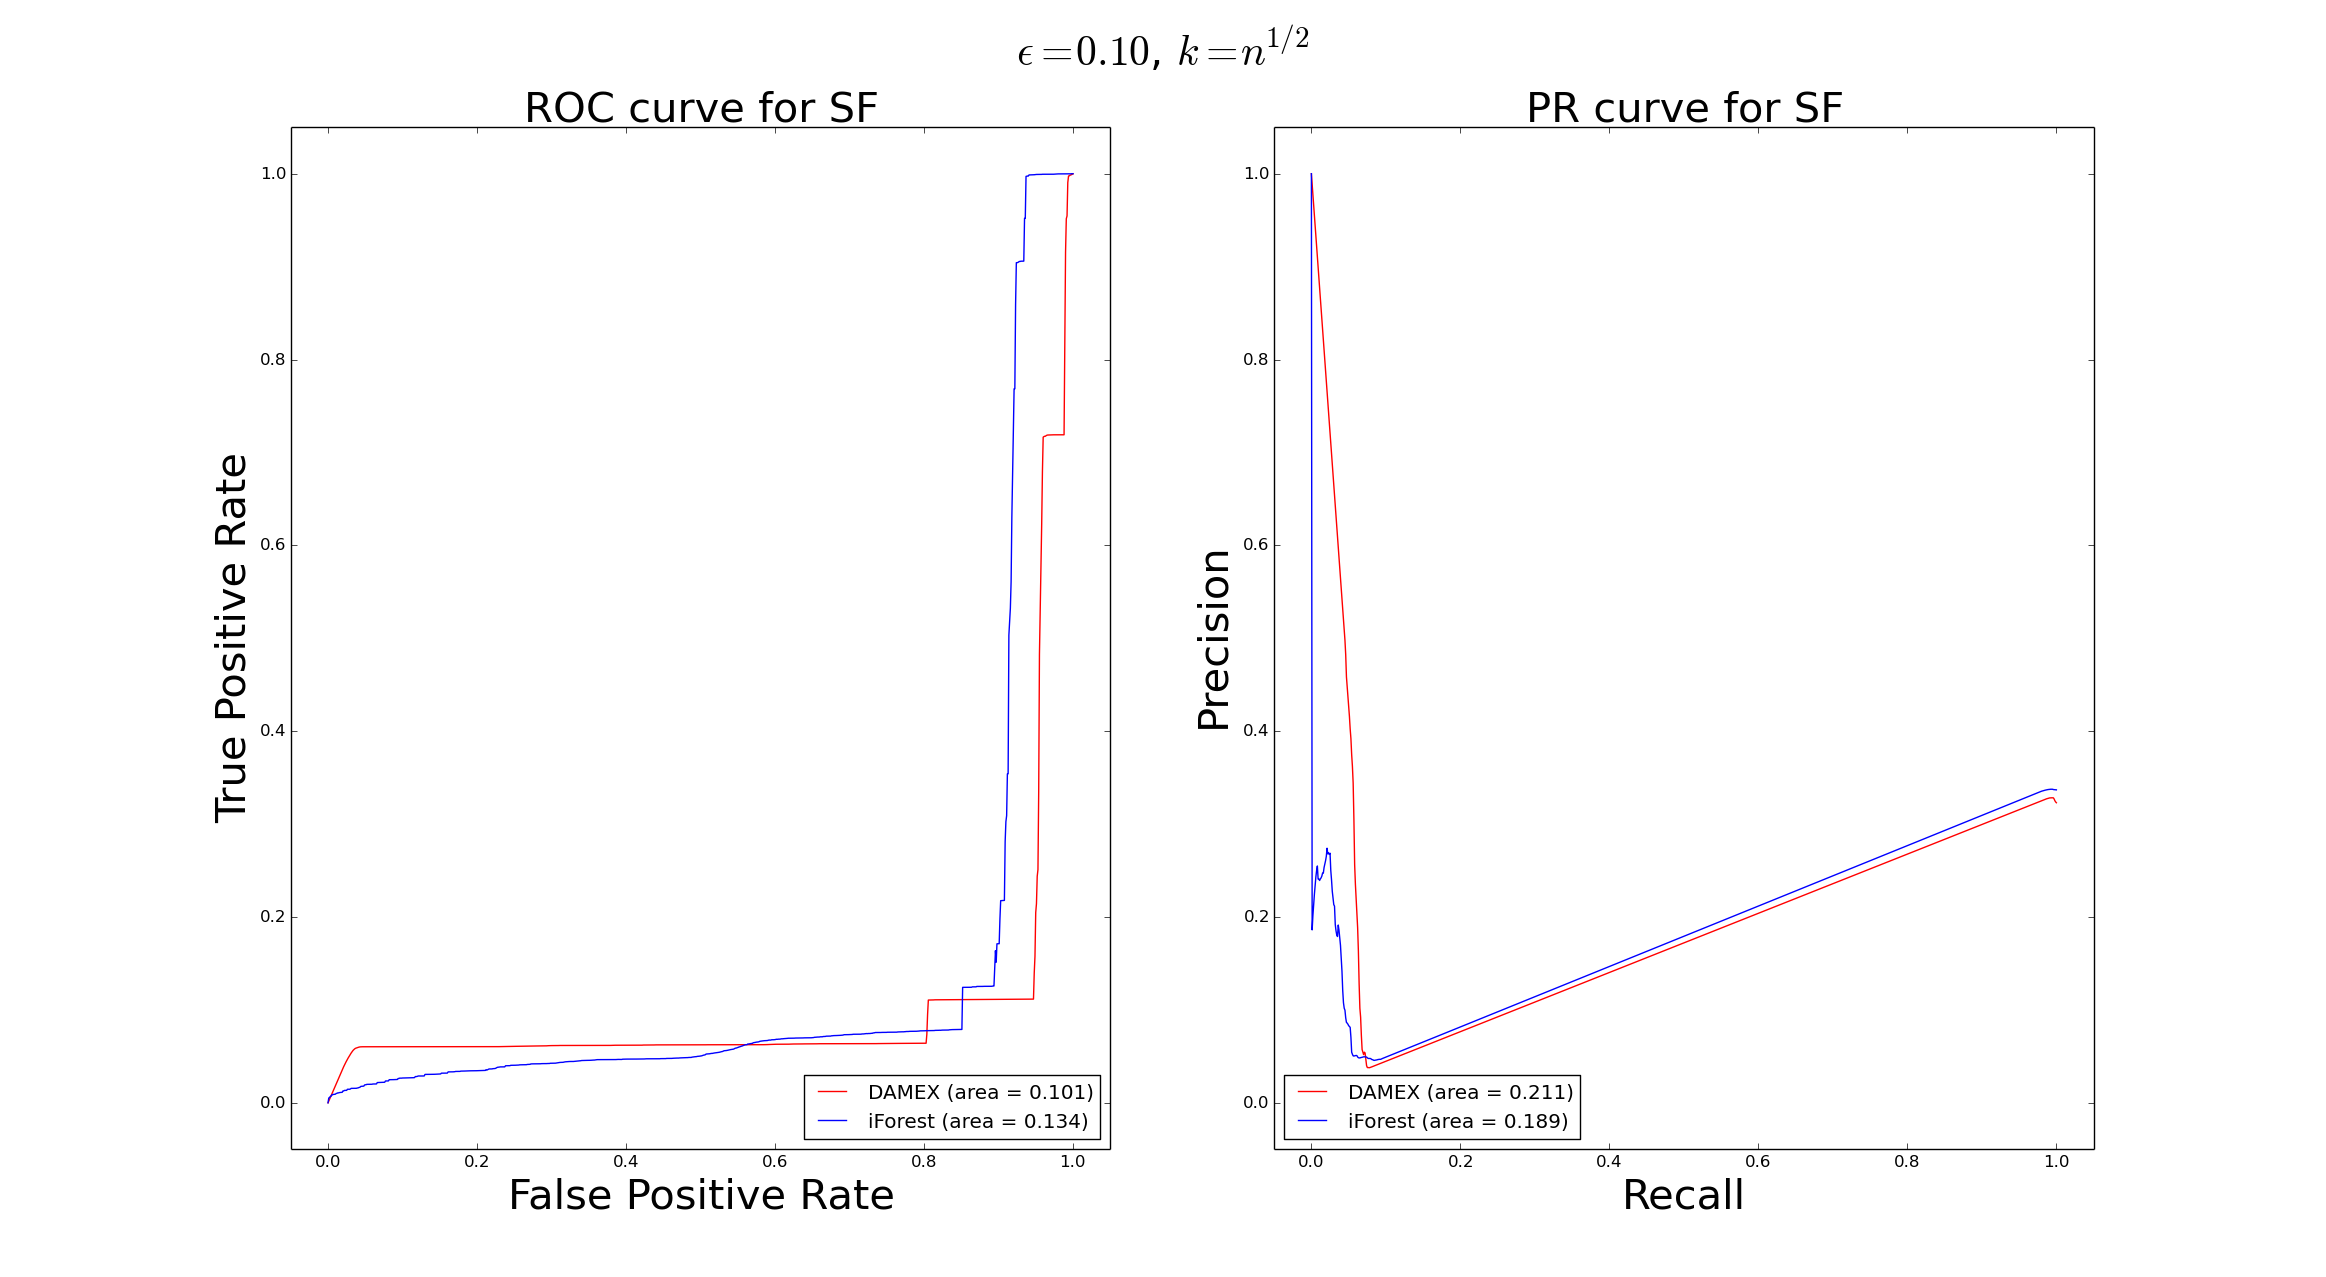
\includegraphics[width = \textwidth]{fig_source/SF-4d-lb-semi-supervised-average-rect-1}
  \caption{SF dataset, larger $\epsilon$}
\label{jmva:fig:SF_1}
\end{figure}

Considering the significant performance improvements on extreme data,
DAMEX may be combined with any standard anomaly detection algorithm to handle extreme
\emph{and} non-extreme data. This would improve the \emph{global}
performance of the chosen standard algorithm, and in particular
decrease the false alarm rate (increase the slope of the ROC curve's tangents near
the origin).  This combination can be done % as illustrated in
% Fig.~\ref{jmva:fig:combination}
by splitting the input space between an
extreme region and a non-extreme one, then using
Algorithm~\ref{jmva:DAMEX-algo} to treat new observations that appear in
the extreme region, and the standard algorithm to deal with those which
appear in the non-extreme region.  % The challenge is then to dovetail
% the two scoring functions obtained, restricted to different
% regions. One way to do it, is to re-scale the scoring function on the
% extreme region from DAMEX, to the (unused) one from the standard
% algorithm on the same region.

% \begin{figure}[!ht]
% \centering
% \includegraphics[scale=0.4]{extreme_AD}
% \caption{Combination of any AD algorithm with DAMEX}
% \label{jmva:fig:combination}
% \end{figure}

\begin{figure}[!ht]
  \centering
  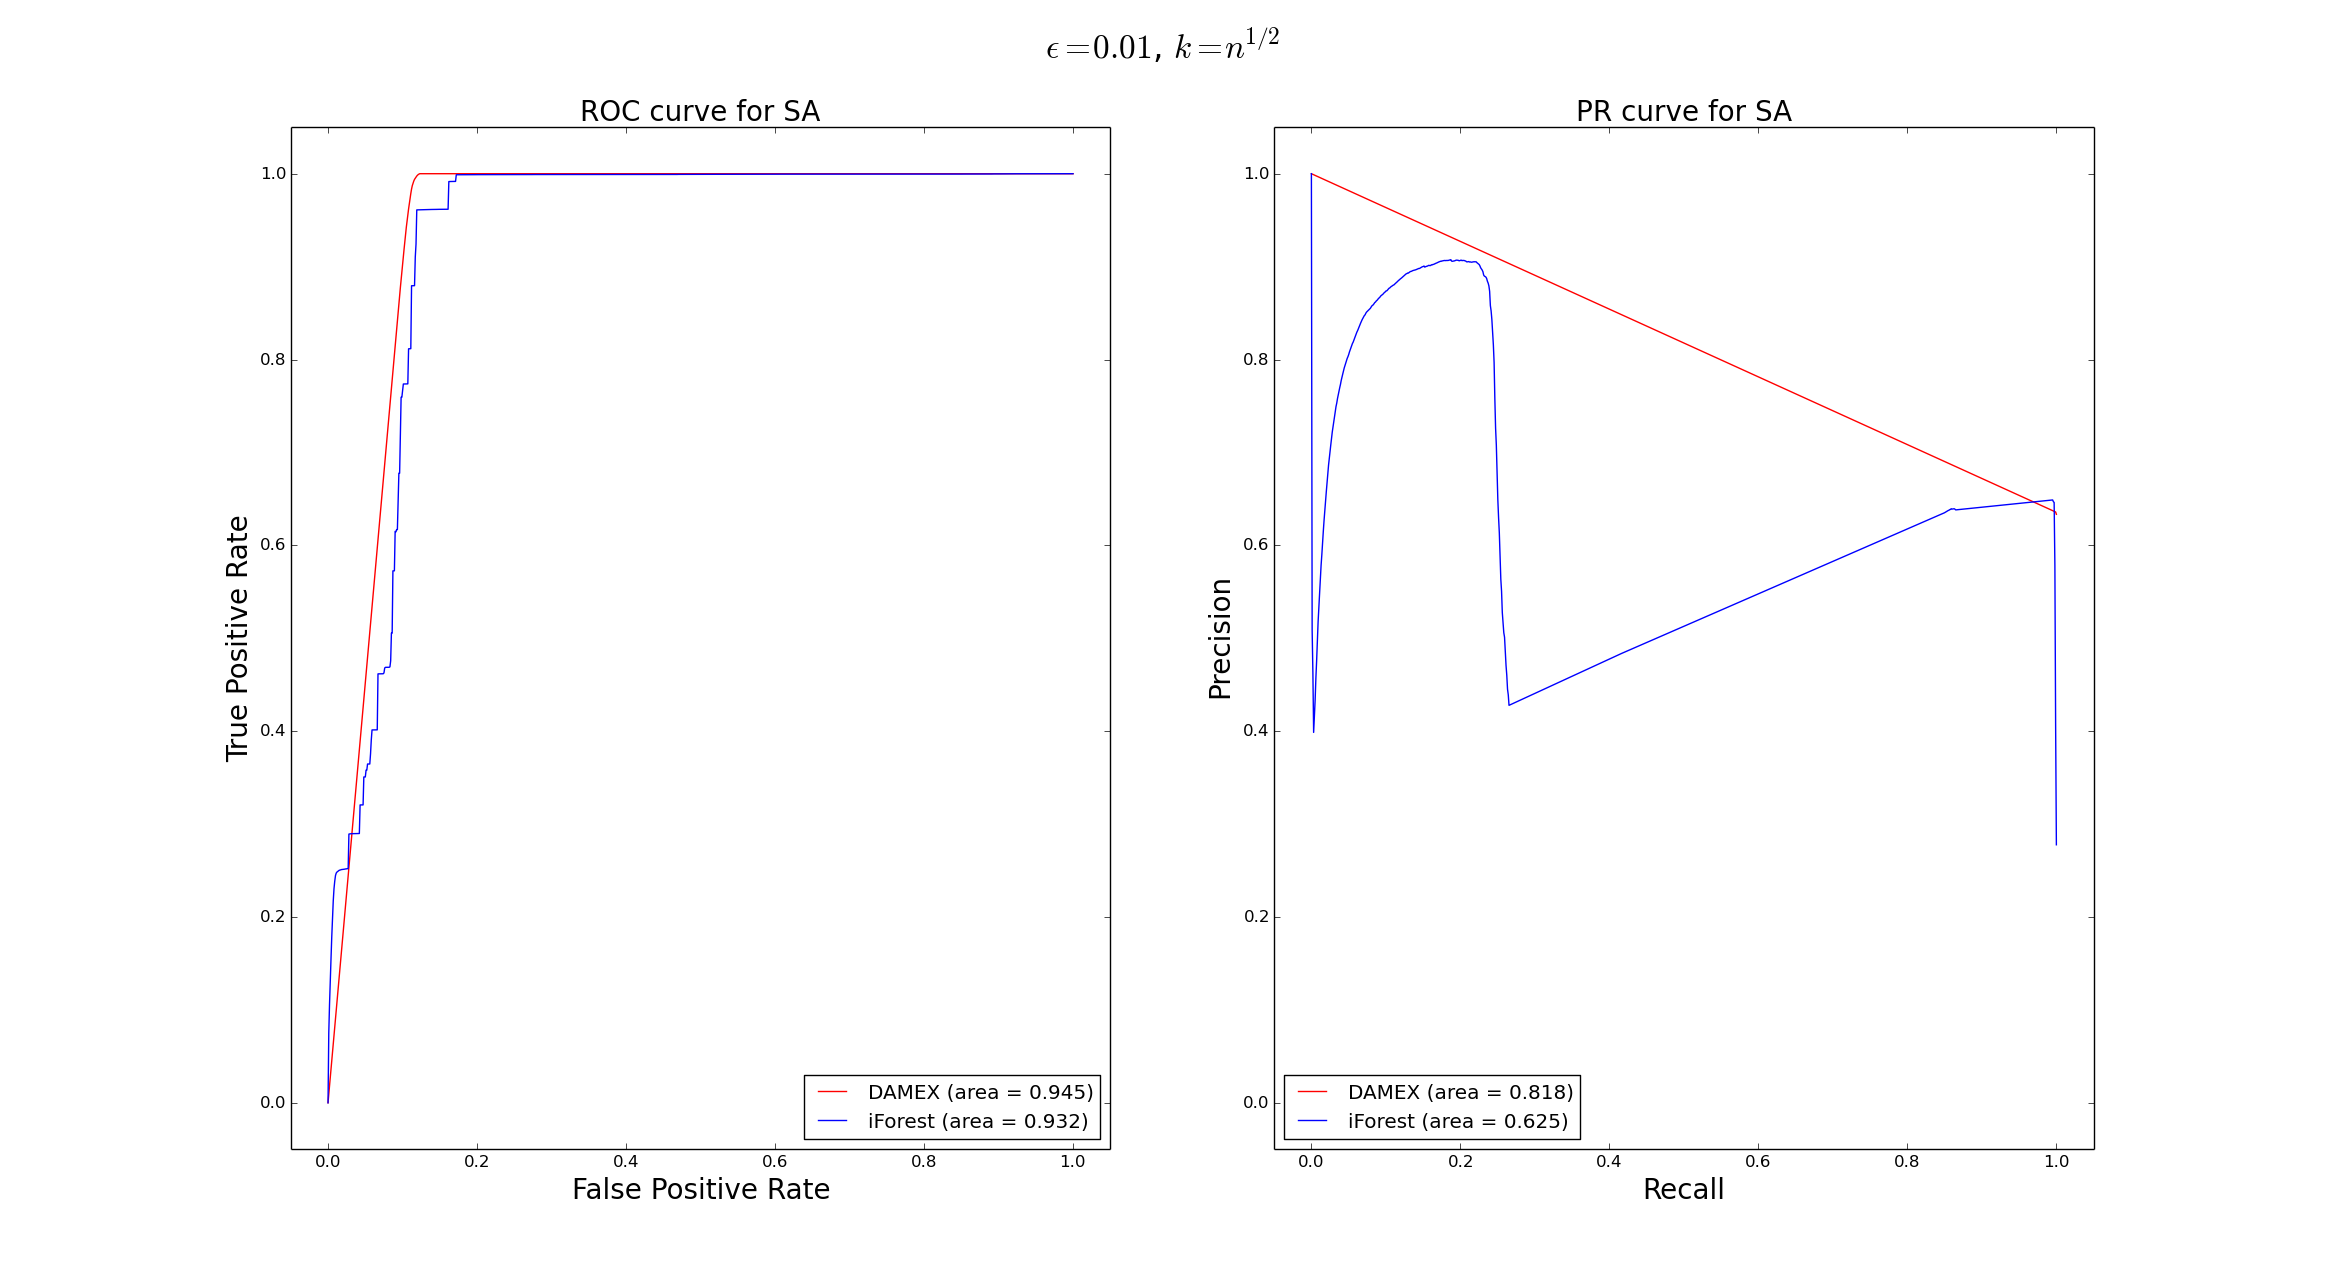
\includegraphics[width = \textwidth]{fig_source/SA-lb-semi-supervised-average-rect-01.png}
  \caption{SA dataset, default parameters}
  \label{jmva:fig:SA}
\end{figure}

\begin{figure}[!ht]
  \centering
  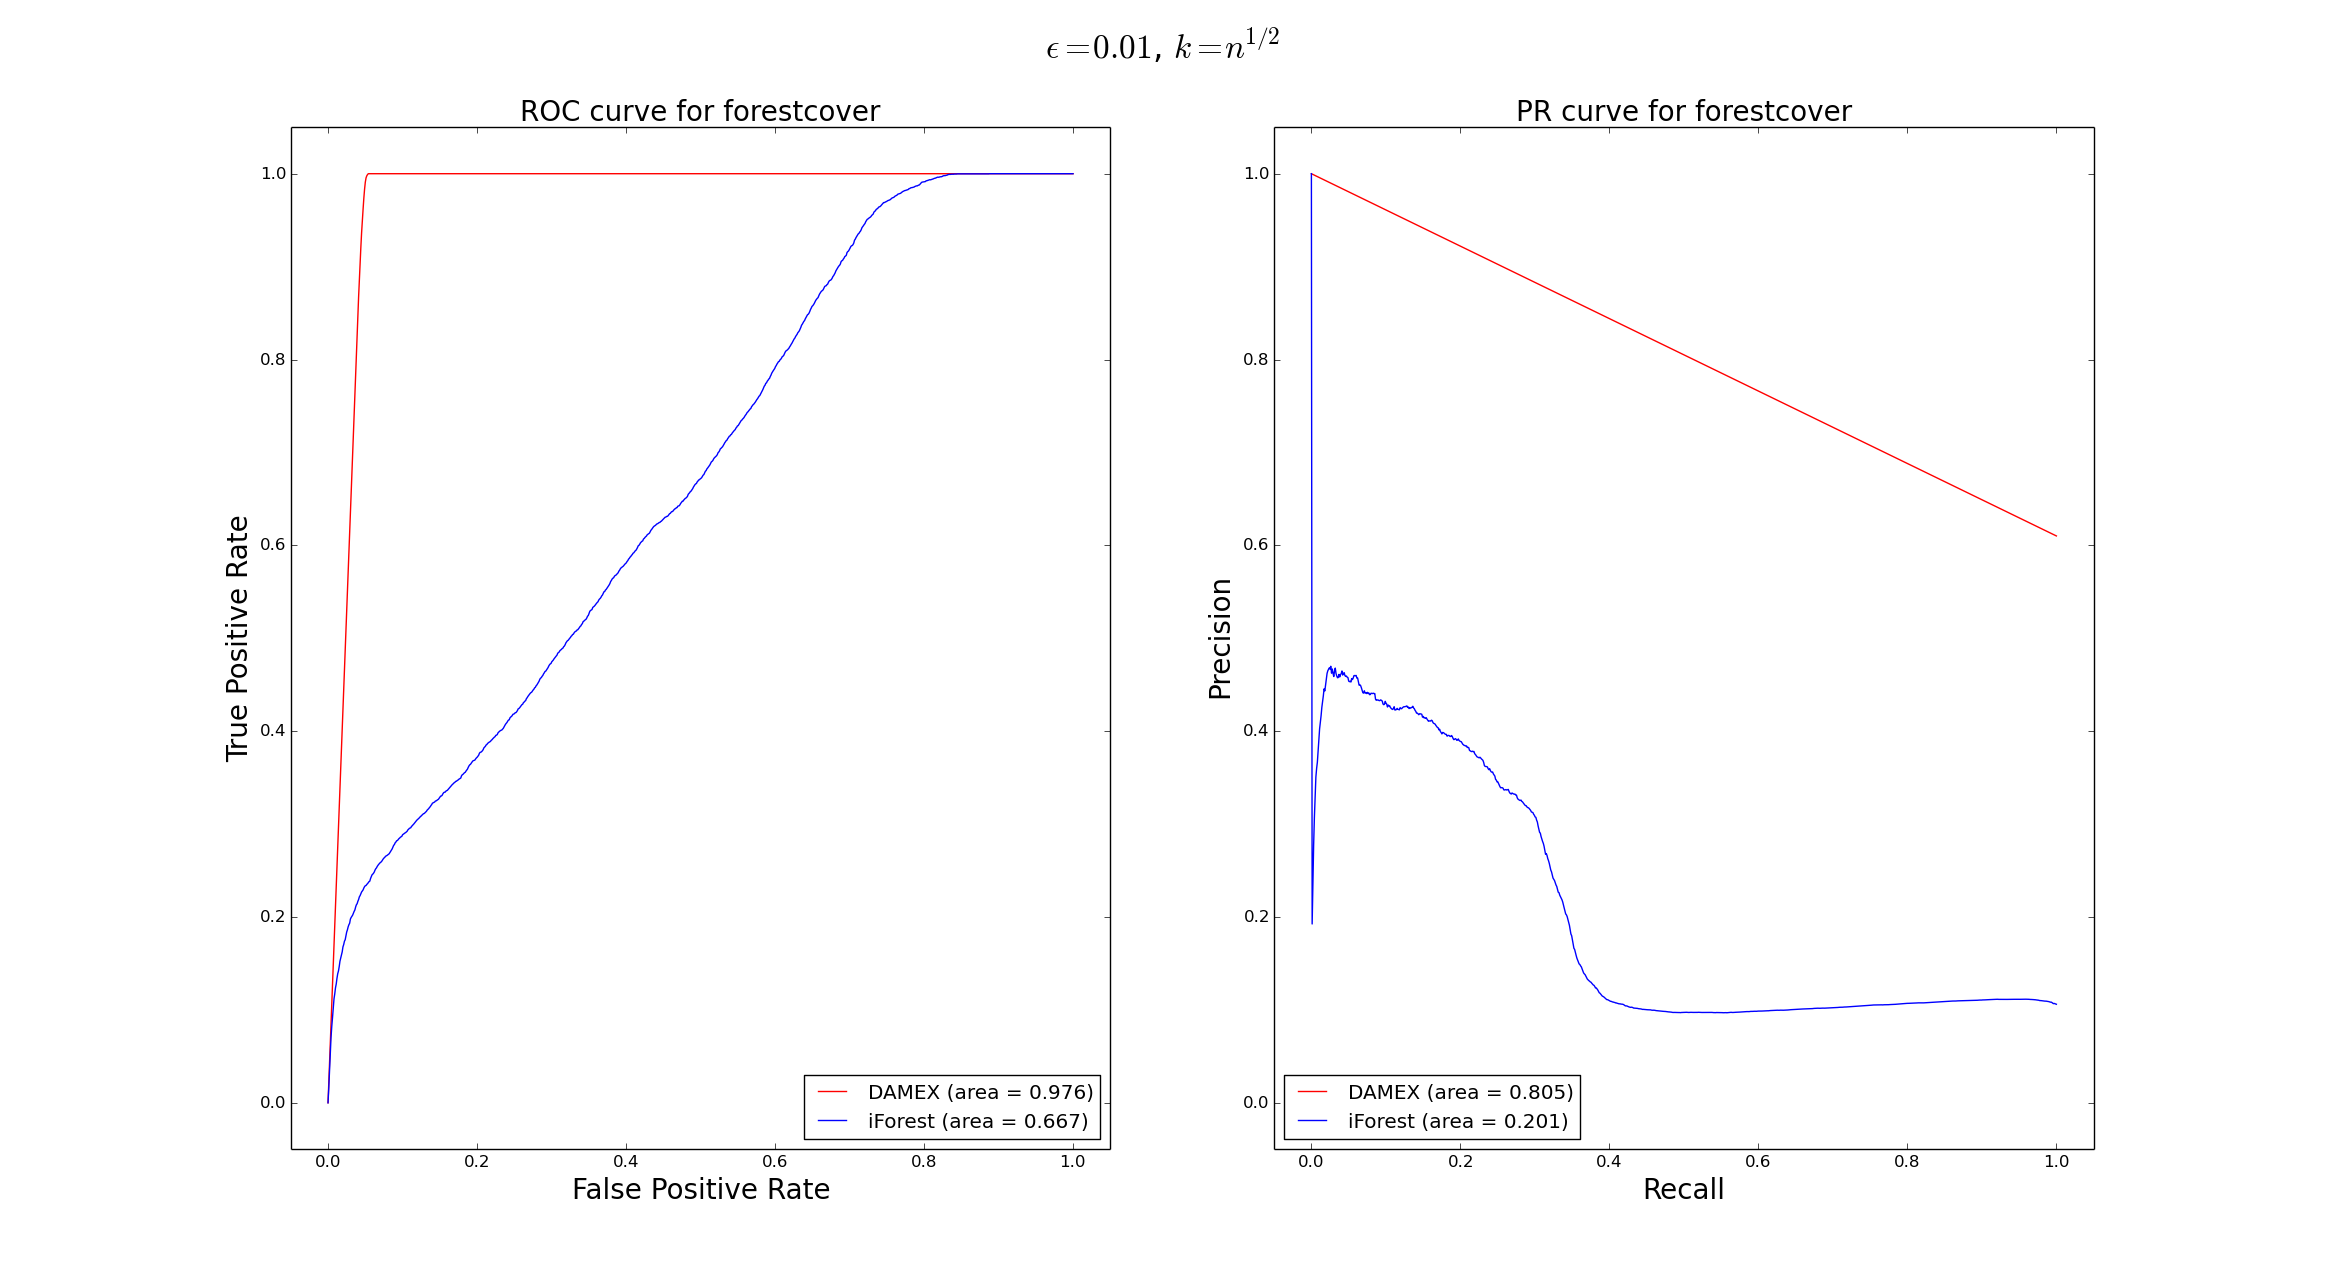
\includegraphics[width = \textwidth]{fig_source/forestcover-semi-supervised-average-rect-01.png}
  \caption{forestcover dataset, default parameters}
\label{jmva:fig:forestcover}
\end{figure}

\begin{figure}[!ht]
  \centering
  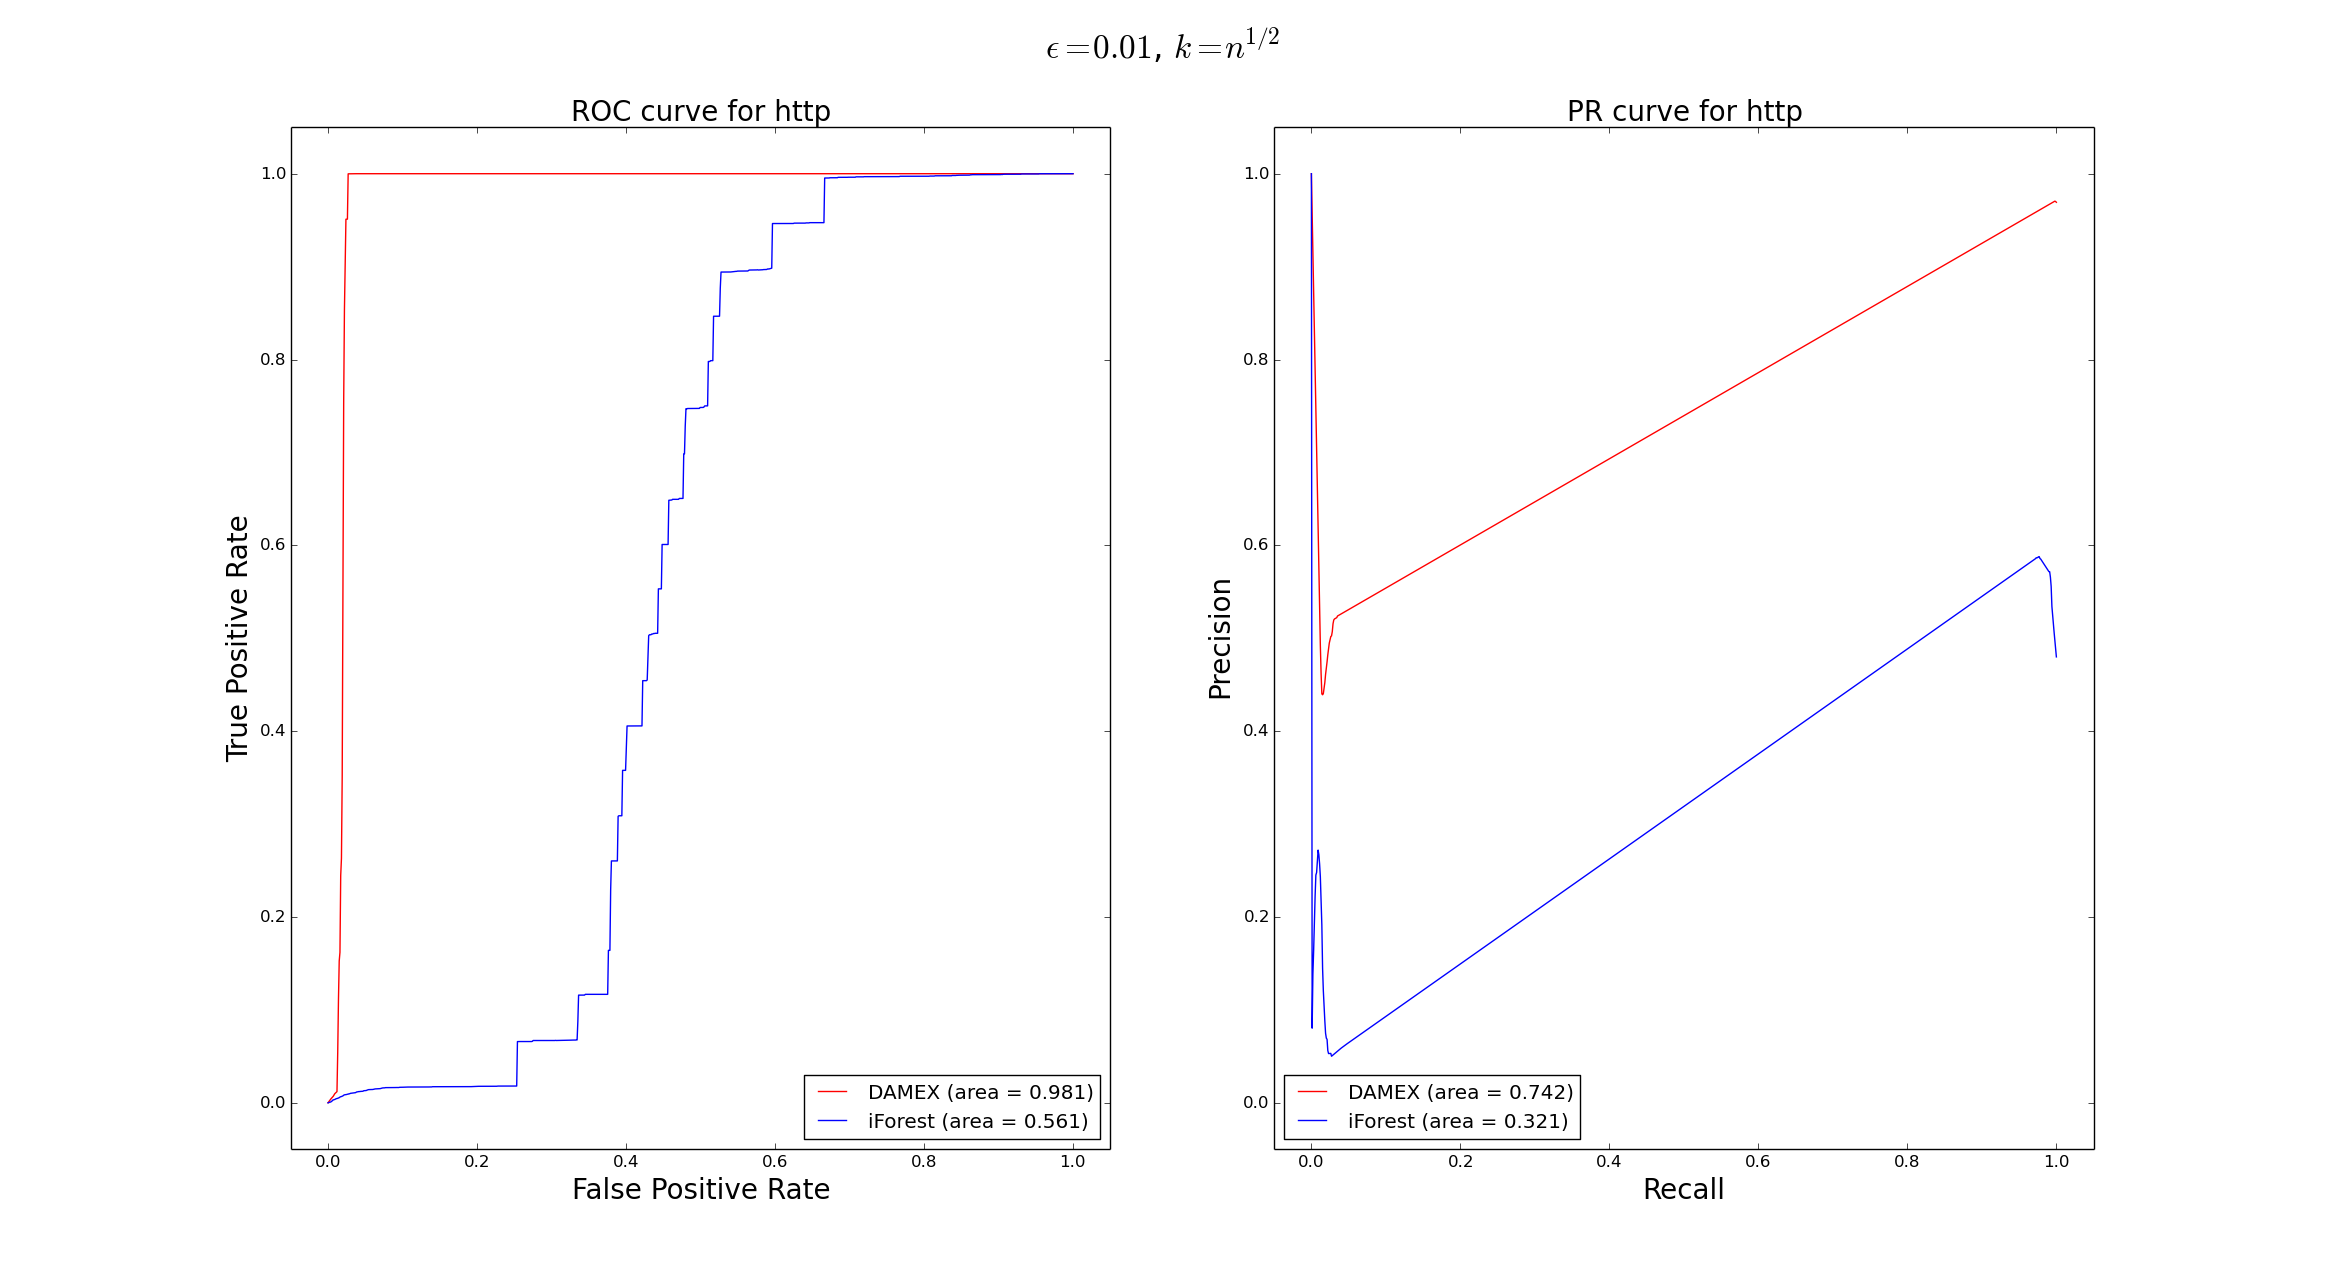
\includegraphics[width = \textwidth]{fig_source/http-3d-semi-supervised-average-rect-01.png}
  \caption{http dataset, default parameters}
\label{jmva:fig:http}
\end{figure}

\section{Conclusion}
The contribution of this chapter is twofold. First, it brings advances in multivariate EVT by designing a statistical method that possibly exhibits a sparsity pattern in the dependence structure of extremes, while deriving non-asymptotic bounds to assess the accuracy of the estimation procedure. Our method is intended to be used as a preprocessing step to scale up multivariate extreme values modeling to high dimensional settings, which is currently one of the major challenges in multivariate EVT.
Since the asymptotic bias ($\text{bias}(\alpha,n,k, \epsilon)$ in eq.~\eqref{jmva:eq:bias}) appears as a separate term  in the bound established, no second order
assumption is required. One possible line of further research would be to make  such an assumption (\ie\,to assume that the bias itself is regularly varying), in order to choose $\epsilon$ adaptively with respect to $k$ and $n$ (see Remark~\ref{jmva:rk_param_choice}). This might also open up the possibility of de-biasing the estimation procedure (\cite{Fougeres2015}, \cite{Beirlant2015}). 
As a second contribution, this work extends the applicability of multivariate  EVT to the field of anomaly detection: a multivariate EVT-based algorithm which scores extreme observations according to their degree of abnormality is proposed. Due to  its  moderate complexity  --of order $d n \log n$--  this algorithm is suitable for the treatment of real word large-scale learning problems, and experimental results reveal a significantly increased performance on extreme regions compared with standard anomaly detection approaches.

%% The Appendices part is started with the command \appendix;
%% appendix sections are then done as normal sections
 
\section{Technical proofs}
\label{jmva:appendix_proof}
\subsection{Proof of Lemma \ref{jmva:lem:equivalence}}
For $n$ vectors $\mb v_1,\ldots,\mb v_n$ in $\mathbb{R}^d$, let us denote by $rank(v_i^j)$ the rank of $v_i^j$ among $v_1^j,\ldots,v_n^j$, that is $rank(v_i^j)=\sum_{k=1}^n \mathds{1}_{\{v_k^j \le v_i^j\}}$, so that $\hat F_j(X_i^j) = (rank(X_i^j)-1)/n$. For the first equivalence, notice that $\hat V_i^j = 1 / \hat U_i^j$.
For the others, we have both at the same time:
\begin{align*}
\hat V_i^j \ge \frac{n}{k} x_j  &~~\Leftrightarrow~~ 1-\frac{rank(X_i^j)-1}{n} ~\le~ \frac{k}{n}~x_j^{-1} 
\\ &~~\Leftrightarrow~~ rank(X_i^j) \ge n-kx_j^{-1} + 1 
\\ &~~\Leftrightarrow~~ rank(X_i^j) \ge n-\lfloor kx_j^{-1}\rfloor + 1 
\\ &~~\Leftrightarrow~~ X_i^j \ge X_{(n-\lfloor kx_j^{-1}\rfloor +1)}^j, 
\end{align*}
and
\begin{align*}
& X_i^j \ge X_{(n-\lfloor  kx_j^{-1} \rfloor +1)}^j ~\Leftrightarrow~
 rank(X_i^j) \ge n-\lfloor  kx_j^{-1} \rfloor+1 \\
&~~~~~~~~~~~~~~~~\Leftrightarrow~  rank( F_j(X_i^j)) \ge n-\lfloor
 kx_j^{-1}\rfloor+1 \qquad(\text{with probability one})\\ 
&~~~~~~~~~~~~~~~~\Leftrightarrow~  rank(1-F_j(X_i^j)) \le \lfloor kx_j^{-1}\rfloor\\
&~~~~~~~~~~~~~~~~\Leftrightarrow~  U_i^j \le U_{(\lfloor kx_j^{-1}\rfloor)}^j.
\end{align*}


\subsection{Proof of Lemma \ref{jmva:lem:g-alpha}}
% First of all, denoting by $A_t$ the event $\bigcap_{j \in \alpha} \left\{ U^j \le t x_j \right\}$ we have:
% \begin{align*}
% \tilde F_{\alpha, \beta} (t \mb x, t \mb z) &~=~ \mathbb{P} \left[ A_t ~~\bigcap~~ \left\{t z_j < U^j  ~~\text{ for } j \in\beta \right\}\right]\\
% &~=~\mathbb{P} \left[ A_t \right] 
% - \mathbb{P} \left[ A_t ~~\bigcap~~ \bigcup_{j \in\beta} \left\{U^j \le t z_j  \right\}\right]
% \end{align*}
% and
% \begin{align*}
% t^{-1}\mathbb{P} \left[ A_t \right] &~~\to~~ \mu\left[\bigcap_{j \in \alpha}\{u,~x_j^{-1} \le u_j\}\right]\\
% t^{-1} \mathbb{P} \left[ A_t ~~\bigcap~~ \bigcup_{j \in\beta} \left\{U^j \le t z_j  \right\}\right]
% &~~\to~~ \mu\left[\bigcap_{j \in \alpha}\{u,~x_j^{-1} \le u_j\} ~~\bigcap~~ \bigcup_{j \in\beta}\{u,~z_j^{-1} \le u_j\}\right]~.
% \end{align*}
% Now, if we denote by $T$ the transformation to polar coordinates, namely $T(u)=(R(u), \Theta(u))$ with $R(u):= \|u\|_\infty$ and $\Theta (u):= \left( \frac{u_1}{R(u)},..., \frac{u_d}{R(u)} \right)$, then
% \begin{align*}
% T \left( \bigcap_{j \in \alpha} \left\{ u,~x_j^{-1} \le u_j\right\} \right) &=  \bigcap_{j \in \alpha}\left\{(r, w),~(w_j x_j)^{-1} \le r \right\} \\
% & =  \left\{ (r, w), ~ \bigvee_{j \in \alpha} (w_j x_j)^{-1} \le r \right\}
% \end{align*}
% so that 
% \begin{align*}
% \mu\left[\bigcap_{j \in \alpha}\left\{u,~x_j^{-1} \le u_j\right\}\right] &= \mu \circ T ^{-1} \left\{(r, w), ~ \bigvee_{j \in \alpha} (w_j x_j)^{-1} \le r \right\} \\
% &= \left( r^{-2}dr \phi \right)  \left\{(r, w), ~ \bigvee_{j \in \alpha} (w_j x_j)^{-1} \le r \right\}\\
% &= \int_{w \in S^{d-1}} \left( \bigvee_{j \in \alpha} (w_j x_j)^{-1} \right)^{-1} \phi(dw)\\
% &= \int_{w \in S^{d-1}}~ \bigwedge_{j \in \alpha} (w_j x_j)~ \phi(dw)~.
% \end{align*}
% Of an analoguous manner we may write:
% \begin{align*}
% &\mu\left[\bigcap_{j \in \alpha}\{u,~x_j^{-1} \le u_j\} ~~\bigcap~~ \bigcup_{j \in\beta}\{u,~z_j^{-1} \le u_j\}\right] \\
% &~~~~~~~~~~~~~~~~~~~~~~~~~~~~~~~=  \mu \circ T ^{-1} \left\{(r, w), ~ \bigvee_{j \in \alpha} (w_j x_j)^{-1} \le r ~~\text{and}~~ \bigwedge_{j \in\beta} (w_j z_j)^{-1} \le r\right\}\\
% &~~~~~~~~~~~~~~~~~~~~~~~~~~~~~~~= \left( r^{-2}dr \phi \right) \left\{(r, w), ~ \max \left( \bigvee_{j \in \alpha} (w_j x_j)^{-1}~,~\bigwedge_{j \in\beta} (w_j z_j)^{-1} \right) \le r\right\}\\
% &~~~~~~~~~~~~~~~~~~~~~~~~~~~~~~~= \int_{w \in S^{d-1}} \left( \max \left( \bigvee_{j \in \alpha} (w_j x_j)^{-1}~,~\bigwedge_{j \in\beta} (w_j z_j)^{-1} \right) \right)^{-1} \phi(dw)\\
% &~~~~~~~~~~~~~~~~~~~~~~~~~~~~~~~= \int_{w \in S^{d-1}} \min \left( \left(\bigvee_{j \in \alpha} (w_j x_j)^{-1}\right)^{-1}~,~\left(\bigwedge_{j \in\beta} (w_j z_j)^{-1}\right)^{-1} \right)  \phi(dw)\\
% &~~~~~~~~~~~~~~~~~~~~~~~~~~~~~~~= \int_{w \in S^{d-1}} \min \left( \bigwedge_{j \in \alpha} w_j x_j~,~\bigvee_{j \in\beta} w_j z_j \right)  \phi(dw)\\
% \end{align*}
% We then obtain:
% \begin{align*}
% g_\alpha(x) = \int_{S^{d-1}} \bigwedge_{j \in \alpha}{w_j x_j}~ \phi(dw) - \int_{S^{d-1}} \min \left(\bigwedge_{j \in \alpha}{w_j x_j}~,~ \bigvee_{j \in\beta} w_j z_j\right) \phi(dw)
% \end{align*}

First, recall that $g_{\alpha,\beta}(\mb x,\mb z) = \mu\big( R(\mb x^{-1},\mb z^{-1}, \alpha,\beta)\big)$, see \eqref{jmva:g_with_mu}. %(this is also valid if some $\alpha_i = 1$, with the convention $\alpha_i^{-1} = +\infty$ is $\alpha = 0$). 
Denote by $\pi$ the transformation to pseudo-polar coordinates introduced
in Section~\ref{jmva:sec:framework}, 
\[
\begin{aligned}
  \pi: [0,\infty]^d \setminus\{\mb 0\} &\to  (0,\infty]\times S^{d-1}_\infty \\
\mb v & \mapsto (r,\boldsymbol{\theta}) = (\|\mb v\|_\infty, \|\mb v\|_\infty^{-1} \mb v). 
\end{aligned}
\]
Then, we have $\ud (\mu \circ\pi^{-1})= \frac{\ud r}{r^2}\ud
\Phi$ on $(0,\infty]\times S^{d-1}_\infty$. This classical result from EVT
comes from the fact that, for $r_0>0$ and $B\subset S^{d-1}_\infty$,  $\mu\circ\pi^{-1}\{ r\ge r_0, \boldsymbol{\theta}\in B\}
= r_0^{-1}\Phi(B)$, see \eqref{jmva:mu-phi}.
Then 
\[
\begin{aligned}
 g_{\alpha,\beta}(\mb x,\mb z)  & = 
\mu\circ\pi^{-1}\Big\{(r,\boldsymbol{\theta}): \quad \forall i \in\alpha,~ r \theta_i \ge
x_i^{-1}\;; \quad \forall j \in\beta, r \theta_j < z_j^{-1} \Big\} \\
&= \mu \circ \pi^{-1} \Big\{(r,\boldsymbol{\theta}): \quad  r  \ge \bigvee_{i\in\alpha}
(\theta_ix_i)^{-1}\;; \quad  r  <\bigwedge_{j\in\beta}(\theta_j z_j)^{-1} \Big\} \\
&= \int_{\boldsymbol{\theta}\in S^{d-1}_\infty} \int_{r>0} \mathds{1}_{r  \ge \bigvee_{i\in\alpha}
(\theta_ix_i)^{-1}}\;\mathds{1}_{r  <\bigwedge_{j\in\beta}(\theta_j
z_j)^{-1}} \frac{\ud r}{r^2} \ud \Phi(\boldsymbol{\theta}) \\ 
& = \int_{\boldsymbol{\theta}\in S^{d-1}_\infty}  \left(
\Big(\bigvee_{i\in\alpha} (\theta_ix_i)^{-1}\Big)^{-1}  - 
\Big(  \bigwedge_{j\in\beta}(\theta_jz_j)^{-1} \Big)^{-1} \right)_+
\ud \Phi(\boldsymbol{\theta}) \\ 
& = \int_{\boldsymbol{\theta}\in S^{d-1}_\infty}  \left(
\bigwedge_{i\in\alpha} \theta_ix_i   - 
 \bigvee_{j\in\beta}\theta_jz_j  \right)_+ \ud \Phi(\boldsymbol{\theta}), \\ 
\end{aligned}
\]
which proves the first assertion. 
To prove the Lipschitz property, notice first that, 
for any finite sequence of real numbers  $c$ and $d$,
$\max_i c_i - \max_i d_i \le \max_i (c_i - d_i)$ and $\min_i c_i -
\min_i d_i \le \max_i (c_i - d_i)$. 
Thus for every $\mb x, \mb z \in [ 0, \infty]^d \setminus \{\boldsymbol{\infty}\}$ and $\theta \in S_\infty^{d-1}$:
\begin{align*}
  &\left(\bigwedge_{j \in \alpha}{\theta_j x_j} - \bigvee_{j \in\beta} \theta_j z_j\right)_+ - \left(\bigwedge_{j \in \alpha}{\theta_j x_j'} - \bigvee_{j \in\beta} \theta_j z_j'\right)_+ \nonumber\\
  &~~~~~~~~~~~~~~~~~~~~~~~~~~~~\le~
 \left[\left(\bigwedge_{j \in \alpha}{\theta_j x_j} -
      \bigvee_{j \in\beta} \theta_j z_j\right) - \left(\bigwedge_{j
        \in \alpha}{\theta_j x_j'} - \bigvee_{j \in\beta} \theta_j
      z_j'\right)\right]_+ \nonumber\\
&~~~~~~~~~~~~~~~~~~~~~~~~~~~~\le~
\left[\bigwedge_{j \in \alpha}{\theta_j x_j} - \bigwedge_{j \in
  \alpha}{\theta_j x_j'} ~+~ \bigvee_{j \in\beta} \theta_j z_j' -
\bigvee_{j \in\beta} \theta_j z_j\right]_+\nonumber\\
&~~~~~~~~~~~~~~~~~~~~~~~~~~~~\le~
    \left[\max_{j \in \alpha}(\theta_j x_j - \theta_j x_j')
      ~+~ \max_{j \in\beta} (\theta_j z_j' - \theta_j z_j) \right]_+ \\%\label{jmva:eq:resultGalpha}\\
 &~~~~~~~~~~~~~~~~~~~~~~~~~~~~\le~
\max_{j \in \alpha}\theta_j|{ x_j} - { x_j'}| ~+~ \max_{j \in\beta} \theta_j | z_j' -  z_j|
\end{align*}
Hence,
\begin{align*}
&|g_{\alpha,\beta}(\mb x, \mb z) - g_{\alpha,\beta}(\mb x', \mb z')|\\
% &~~~~~~~~~~~~~~~~~~~~~~\le~ \int_{S^{d-1}_\infty} \left(\max_{j \in \alpha}|{\theta_j x_j} -
%   {\theta_j x_j'}| ~+~ \max_{j \in\beta} |\theta_j z_j' - \theta_j
%   z_j|\right) \ud \Phi(\boldsymbol{\theta}). \\
&~~~~~~~~~~~~~~~~~~~~~~~\le~\int_{S^{d-1}_\infty} \left(\max_{j \in \alpha}\theta_j|{ x_j} - { x_j'}| ~+~ \max_{j \in\beta} \theta_j | z_j' -  z_j|\right)  \ud\Phi(\boldsymbol{\theta})~.
\end{align*}
Now, by \eqref{jmva:eq:integratePhiLambda} we have:
$$\int_{S^{d-1}_\infty} \max_{j \in \alpha}\theta_j|{ x_j} - { x_j'}| ~~ \ud\Phi(\boldsymbol{\theta}) = \mu([\mb 0, \mb{\tilde x}^{-1}]^c)$$ with $\mb{\tilde x}$ defined as $\tilde x_j = |x_j - x_j'|$ for $j\in\alpha$, and $0$ elsewhere.
It suffices then to write:
\begin{align*}
\mu([\mb 0, \mb{\tilde x}^{-1}]^c) &= \mu(\{y,~\exists j \in \alpha,~y_j \ge |x_j-x_j'|^{-1}\})\\
 &\le \sum_{j\in\alpha}\mu(\{y,~y_j \ge |x_j-x_j'|^{-1}\})\\
 &\le \sum_{j \in \alpha} |x_j-x_j'|~.
\end{align*}
Similarly, $\int_{S^{d-1}_\infty} \max_{j \in\beta} \theta_j | z_j' -  z_j|  ~~ \ud\Phi(\boldsymbol{\theta}) ~\le~ \sum_{j \in \beta} |z_j-z_j'|$.

%
% Now, following
% the same argument as that leading to (\ref{jmva:eq:resultGalpha}), one obtains that $\mu\{ \mb v: v_j\ge 1\}  =
% \int_{S^{d-1}_\infty} \theta_j \ud\Phi(\boldsymbol{\theta})$.
% Since our marginal standardization choice  implies $\mu\{\mb v:
% v_j\ge 1\} = 1$, we get that 
% \begin{align*}
% |g_{\alpha,\beta}(\mb x, \mb z) - g_{\alpha,\beta}(\mb x', \mb z')|\le\|\mb x - \mb x'\|_\infty + \|\mb z - \mb z'\|_\infty ~\le \|\mb x - \mb x'\|_1 + \|\mb z - \mb z'\|_1.
% \end{align*}


\subsection{Proof of Proposition \ref{jmva:prop:g}}
%For notational convenience, we denote by $\max_\alpha$ the maximum taken on $\{\alpha \subset \{1,...d\} \setminus \emptyset \}$.
The starting point is inequality (9) on p.7 in \cite{COLT15} which bounds the deviation of the empirical measure on extreme regions. 
%Consider a random vector $\mathbf{Z}=(Z^1,\ldots,Z^d)$ with uniform margins on $[0,1]$,
Let $\mathcal{C}_n(\point)=\frac{1}{n} \sum_{i=1}^{n} \mathds{1}_{\{\mb Z_i \in \point \}}$ 
% (the $\mb Z_i$'s are \iid~realizations of $\mb Z$ )
and $\mathcal{C}(\mathbf{x})=\mathbb{P}(\mb Z \in \point)$ be the empirical and true measures associated with a n-sample $\mb Z_1, \ldots, \mb Z_d$ of \iid~realizations of a random vector $\mathbf{Z}=(Z^1,\ldots,Z^d)$ with uniform margins on $[0,1]$. Then for any real number $\delta \ge e^{-k}$, 
with probability greater than $1 - \delta$,
\begin{align}
\label{jmva:Qialt2}
\sup_{0 \le \mathbf{x} \le T} \frac{n}{k} \left | \mathcal{C}_n(\frac{k}{n} [\mathbf{x},\boldsymbol{\infty}[^c) - \mathcal{C}(\frac{k}{n} [\mathbf{x},\boldsymbol{\infty}[^c)  \right| ~\le~ C d\sqrt{\frac{T}{k} \log{\frac{1}{\delta}}}~.
\end{align} 
Recall that with the above notations, $0 \le \mb x \le T$ means $0 \le x_j \le T$ for every $j$.
The proof of Proposition~\ref{jmva:prop:g} follows the same lines as in \cite{COLT15}. 
The cornerstone concentration inequality \eqref{jmva:Qialt2} has to be replaced with 
\begin{align}
\label{jmva:cornerstone-extension}
\nonumber \max_{\alpha, \beta} \sup_{\substack{  0 \le \mb x, \mb z \le T \\ \exists j \in \alpha, x_j \le T'}}
&\frac{n}{k} \left | \mathcal{C}_n \left(\frac{k}{n} R(\mb x^{-1}, \mb z^{-1}, \alpha,~\beta)^{-1}\right) - \mathcal{C}\left(\frac{k}{n} R(\mb x^{-1}, \mb z^{-1}, \alpha,~\beta)^{-1}\right)  \right|\\
&~~~~~~~~~~~~~~~~~~~~~~~~~~~~~~~~~~~~~~~~~ ~\le~ Cd \sqrt{\frac{dT'}{k} \log{\frac{1}{\delta}}}~.
\end{align}
\begin{remark}
Inequality \eqref{jmva:cornerstone-extension} is here written in its full generality, namely with a separate constant $T'$ possibly smaller than $T$. If $T' < T$, we then have a smaller bound (typically, we may use $T = 1/\epsilon$ and $T' = 1$). However, we only use \eqref{jmva:cornerstone-extension} with $T = T'$ in the analysis below, since the smaller bounds in $T'$ obtained (on $\Lambda(n)$ in \eqref{jmva:proof_decomp}) would be diluted (by $\Upsilon(n)$ in \eqref{jmva:proof_decomp}).
\end{remark}
\begin{proof}[Proof of (\ref{jmva:cornerstone-extension})]
Recall that for notational convenience we write `$\alpha,\beta$' for `$\alpha$ non-empty subset of $ \{1,\ldots,d\}$ and $\beta$ subset of $ \{1,\ldots,d\}$'.
% Inequality \eqref{jmva:cornerstone-extension} is obtained by using
The key is to apply Theorem 1 in \cite{COLT15}, with a VC-class which fits our purposes. Namely, consider
\begin{align*}
\mathcal{A} ~~=~~ \mathcal{A}_{T,T'} ~~&=~~ \bigcup_{\alpha, \beta} \mathcal{A}_{T,T',\alpha,\beta} \text{~~~~~with}\\
\mathcal{A}_{T,T',\alpha,\beta} ~~=~~& \frac{k}{n}\Big\{ R(\mb x^{-1}, \mb z^{-1}, \alpha,~\beta)^{-1}:~~ \mb x, \mb z \in \mathbb{R}^d ,~ 0 \le \mb x, \mb z \le T,\\
&~~~~~~~~~~~~~~~~~~~~~~~~~~~~~~~~~~~~~~~~~~~~~~~~~~~~~~~~\exists j \in \alpha, x_j \le T' \Big\}~,
\end{align*}
for $T,~T' > 0$ and $\alpha,~\beta \subset \dd,~\alpha \neq \emptyset$. $\mathcal{A}$ has VC-dimension $V_\mathcal{A} = d$, as the one considered in \cite{COLT15}. Recall in view of (\ref{jmva:set-R}) that 
\begin{align*}
R(\mb x^{-1}, \mb z^{-1}, \alpha,~\beta)^{-1} ~&=~ \Big\{ \mb y \in [0, \infty]^d , ~~y_j \le x_j ~~\text{ for } j \in \alpha,\\
&~~~~~~~~~~~~~~~~~~~~~~~~~  y_j > z_j ~~\text{ for } j \in\beta ~~\Big\} \\&=~ [\mb a, \mb b],
\end{align*}
with $\mb a$ and $\mb b$ defined by 
$a_j =   \left \lbrace \begin{array}{cc}
0 &  \text{for} ~ j \in \alpha \\
z_j  & \text{for} ~ j \in\beta \\
\end{array}
\right.$
and
$b_j =   \left \lbrace \begin{array}{cc}
x_j &  \text{for} ~ j \in \alpha \\
\infty  & \text{for} ~ j \in\beta \\
\end{array}
\right.$.
Since we have $\forall A \in \mathcal{A}, A \subset [\frac{k}{n} \mb T',~\boldsymbol{\infty}[^c$, the probability for a \rv~$\mb Z$ with uniform margins in $[0,1]$ to be in the union class $\mathbb{A} = \bigcup_{A \in \mathcal{A}}A$ is $\mathbb{P}(\mb Z \in \mathbb{A}) \le \mathbb{P}(\mb Z \in [\frac{k}{n}\mb T',~\boldsymbol{\infty}[^c) \le \sum_{j=1}^d \mathbb{P}(Z^j \le \frac{k}{n} T') \le \frac{k}{n}dT'$. 
Inequality \eqref{jmva:cornerstone-extension} is thus a direct consequence of Theorem 1 in \cite{COLT15}.
\end{proof}
\noindent
Define now the empirical version $\tilde F_{n, \alpha, \beta}$ of $\tilde F_{\alpha, \beta}$ (introduced in (\ref{jmva:F-tilde-alpha})) as 
\begin{align}
\label{jmva:def:Fn}
\tilde F_{n, \alpha, \beta}(\mb x, \mb z)  ~=~ \frac{1}{n} \sum_{i=1}^n \mathds{1}_{\{ U_i^j \le x_j ~~\text{for}~ j \in \alpha ~~\text{ and }~~  U_i^j > z_j ~~\text{for}~ j \in\beta \}}~ ,
\end{align}
so that 
$  \frac{n}{k} \tilde F_{n, \alpha, \beta}( \frac{k}{n} \mb x, \frac{k}{n} \mb z) ~=~ \frac{1}{k} \sum_{i=1}^n 
\mathds{1}_{\{ U_i^j \le \frac{k}{n} x_j ~~\text{for}~ j \in \alpha ~~\text{ and }~~ U_i^j > \frac{k}{n} z_j   ~~\text{for}~ j \in\beta \}}.$
Notice that the $U_i^j$'s are  not observable (since $F_j$ is
unknown). In fact, $\tilde F_{n, \alpha, \beta}$ will be used as a substitute for $g_{n, \alpha, \beta}$ (defined in \eqref{jmva:def:gn}) allowing to handle uniform variables. This is illustrated by the following lemmas. 

\begin{lemma}[Link between $g_{n, \alpha, \beta}$ and $\tilde F_{n, \alpha, \beta}$]
\label{jmva:lem:gn-Fn}
The  empirical version of $\tilde F_{\alpha, \beta}$ and that of $g_{\alpha, \beta}$ are related \emph{via}
\begin{align*}
g_{n, \alpha, \beta}(\mb x, \mb z)~=~\frac{n}{k} \tilde F_{n, \alpha, \beta}\left( \left(U_{(\lfloor kx_j\rfloor)}^j\right)_{j \in \alpha} , \left(U_{(\lfloor kz_j\rfloor)}^j\right)_{j \in \beta}\right),
\end{align*}
\end{lemma}

\begin{proof}
Considering the definition in (\ref{jmva:def:Fn}) and (\ref{jmva:eq:gn2}), both sides are equal to $\mu_n(R(\mathbf{x}^{-1}, \mathbf{z}^{-1}, \alpha,\beta))$. %by Lemma \ref{jmva:lem:equivalence}.
\end{proof}


\begin{lemma}[Uniform bound on $\tilde F_{n, \alpha, \beta}$'s deviations]
\label{jmva:lem:Fn-tildeF}
 For any finite  $T>0$, and $\delta\ge e^{-k}$,  with probability at least $1-\delta$, the  deviation of $\tilde F_{n, \alpha, \beta}$ from  $\tilde F_{\alpha, \beta}$ is uniformly bounded: % independently of $\alpha$ and $\beta$:
 
\begin{align*}
\max_{\alpha, \beta} \sup_{ 0 \le \mb x, \mb z \le T}
\left| \frac{n}{k} \tilde F_{n, \alpha, \beta}( \frac{k}{n} \mb x, \frac{k}{n} \mb z)-\frac{n}{k} \tilde F_{\alpha, \beta}( \frac{k}{n} \mb x, \frac{k}{n} \mb z) \right| \le Cd\sqrt{\frac{T}{k}\log{\frac{1}{\delta}}}~.
\end{align*}
\end{lemma}
\begin{proof}
Notice that 
\begin{align*}
&\sup_{ 0 \le \mb x, \mb z \le T} \left| \frac{n}{k} \tilde F_{n, \alpha, \beta}( \frac{k}{n} \mb x, \frac{k}{n} \mb z)- \frac{n}{k} \tilde F_{\alpha, \beta}( \frac{k}{n} \mb x, \frac{k}{n} \mb z) \right|  \\
&~= \sup_{ 0 \le \mb x, \mb z \le T} \frac{n}{k} \left|  \frac{1}{n}  \sum_{i=1}^n \mathds{1}_{ \mb U_i \in \frac{k}{n} R(\mb x^{-1}, \mb z^{-1}, \alpha,~\beta)^{-1} } -
   \mathbb{P} \left[ \mathbf{U} \in \frac{k}{n} R(\mb x^{-1}, \mb z^{-1}, \alpha,~\beta)^{-1}
   \right] \right|,
\end{align*}
and apply inequality (\ref{jmva:cornerstone-extension}) with $T'=T$.
\end{proof}
%
\begin{remark}
%\label{jmva:rk:prop:g_generalized}
\label{jmva:rk:lem:Fn-tildeF_generalized}
% For each $n>0$, with probability at least $1 - \delta$,~ for each $\alpha \subset\{1,\ldots,d\}\setminus \emptyset$ and $\beta \subset\{1,\ldots,d\}$,
% \begin{align*}
% \sup_{\substack{  0 \le \mb x, \mb z \le T \\ \exists j \in \alpha, x_j \le T'}} \left| g_{n, \alpha, \beta}(\mb x, \mb z) - g_{\alpha, \beta}(\mb x, \mb z) \right| &~\le~  Cd\sqrt{\frac{2T'}{k}\log\frac{d+3}{\delta}} 
% \\\nonumber &~~~~~~+ \sup_{0 \le \mb x, \mb z \le 2T}\left|\frac{n}{k} \tilde F_{\alpha, \beta}( \frac{k}{n} \mb x, \frac{k}{n} \mb z)- g_{\alpha, \beta}(\mb x, \mb z)\right|.
% \end{align*}
Note that the following stronger inequality holds true, when using (\ref{jmva:cornerstone-extension}) in full generality, \ie~with $T'< T$.
 For any finite  $T, T'>0$, and $\delta\ge e^{-k}$,  with probability at least $1-\delta$,
\begin{align*}
\max_{\alpha, \beta} \sup_{\substack{  0 \le \mb x, \mb z \le T \\ \exists j \in \alpha, x_j \le T'}}
\left| \frac{n}{k} \tilde F_{n, \alpha, \beta}( \frac{k}{n} \mb x, \frac{k}{n} \mb z)-\frac{n}{k} \tilde F_{\alpha, \beta}( \frac{k}{n} \mb x, \frac{k}{n} \mb z) \right| \le Cd\sqrt{\frac{T'}{k}\log{\frac{1}{\delta}}}.
\end{align*}
\end{remark}

The following lemma is stated and proved in \cite{COLT15}.
\begin{lemma}[Bound on the order statistics of $\mb U$]
\label{jmva:lem:U-x} 
Let $\delta\ge e^{-k}$. For any finite positive number $T>0$ such that $T \ge 7/2((\log d)/k + 1)$, we have with probability greater than $1 - \delta$, 
\begin{align}
\label{jmva:lem:eq-Wellner}
\forall~ 1\le j \le d,~~~~~\frac{n}{k} U_{(\lfloor kT\rfloor )}^j ~\le~ 2T~,
\end{align}
and with probability greater than $1- (d+1)\delta$, 
\begin{align*}
\max_{1 \le j \le d}~ \sup_{0 \le x_j \le T} \left| \frac{\lfloor kx_j\rfloor }{k} - \frac{n}{k} U_{(\lfloor kx_j\rfloor )}^j  \right| ~\le~ C\sqrt{\frac{T}{k}\log{\frac{1}{\delta}}}~.
\end{align*}
\end{lemma}
\noindent
We may now proceed with the proof of Proposition \ref{jmva:prop:g}.
Using Lemma \ref{jmva:lem:gn-Fn}, we may write:
\begin{align}
\nonumber &\max_{\alpha, \beta}\sup_{ 0 \le \mb x, \mb z \le T }
 \left| g_{n, \alpha, \beta}(\mb x, \mb z) - g_{\alpha, \beta}(\mb x, \mb z) \right| \\
\nonumber           &~~~~~~~~~~=~ \max_{\alpha, \beta}  \sup_{ 0 \le \mb x, \mb z \le T } \left| \frac{n}{k} \tilde F_{n, \alpha, \beta} \left( \left(U_{(\lfloor kx_j\rfloor)}^j\right)_{j \in \alpha} , \left(U_{(\lfloor kz_j\rfloor)}^j\right)_{j \in \beta} \right) - g_{\alpha, \beta}(\mb x, \mb z) \right| \\
\label{jmva:proof_decomp}&~~~~~~~~~~\le~ \Lambda(n) ~+~ \Xi(n) ~+~ \Upsilon(n)~.
\end{align}
with:
\begin{align*}
 \Lambda(n) &~=~ \max_{\alpha, \beta} \sup_{ 0 \le \mb x, \mb z \le T } \bigg| \frac{n}{k} \tilde F_{n, \alpha, \beta} \left(\left(U_{(\lfloor kx_j\rfloor)}^j\right)_{j \in \alpha} , \left(U_{(\lfloor kz_j\rfloor)}^j\right)_{j \in \beta} \right) 
\\&~~~~~~~~~~~~~~~~~~~~~~~~~~~~~~~~~~~~~~~- \frac{n}{k} \tilde F_{\alpha, \beta} \left(\left(U_{(\lfloor kx_j\rfloor)}^j\right)_{j \in \alpha} , \left(U_{(\lfloor kz_j\rfloor)}^j\right)_{j \in \beta} \right)  \bigg|\\
\Xi(n) &~=~\max_{\alpha, \beta} \sup_{0 \le \mb x, \mb z \le T} \bigg| \frac{n}{k} \tilde F_{\alpha, \beta} \left(\left(U_{(\lfloor kx_j\rfloor)}^j\right)_{j \in \alpha} , \left(U_{(\lfloor kz_j\rfloor)}^j\right)_{j \in \beta} \right)
\\&~~~~~~~~~~~~~~~~~~~~~~~~~~~~~~~~~~~~~- g_{\alpha, \beta}\left(\left(\frac{n}{k}U_{(\lfloor kx_j\rfloor)}^j\right)_{j \in \alpha} , \left(\frac{n}{k}U_{(\lfloor kz_j\rfloor)}^j\right)_{j \in \beta}\right) \bigg|\\
\Upsilon(n) &~=~ \max_{\alpha, \beta} \sup_{ 0 \le \mb x, \mb z \le T } \left| g_{\alpha, \beta}\left(\left(\frac{n}{k}U_{(\lfloor kx_j\rfloor)}^j\right)_{j \in \alpha} , \left(\frac{n}{k}U_{(\lfloor kz_j\rfloor)}^j\right)_{j \in \beta}\right) - g_{\alpha, \beta}(\mb x, \mb z) \right|.
\end{align*}
Now, considering (\ref{jmva:lem:eq-Wellner}) we have with probability greater than $1-\delta$ that
for every $1\le j \le d$, $U_{(\lfloor kT\rfloor )}^j ~\le~ 2T \frac{k}{n}~$, so that
\begin{align*} 
\Lambda(n) % &~\le~
% \max_{\alpha, \beta}  \sup_{ 0 \le \mb x, \mb z \le T } \bigg| \frac{n}{k} \tilde F_{n, \alpha, \beta}  \left(
% \left(U_{(\lfloor kx_j\rfloor)}^j\right)_{j \in \alpha} , \left(U_{(\lfloor kz_j\rfloor)}^j\right)_{j \in \beta} \right) 
% \\&~~~~~~~~~~~~~~~~~~~~~~~~~~~~~~~~~~~~~~~~- \frac{n}{k} \tilde F_{\alpha, \beta}  \left(\left(U_{(\lfloor kx_j\rfloor)}^j\right)_{j \in \alpha} , \left(U_{(\lfloor kz_j\rfloor)}^j\right)_{j \in \beta} \right)  \bigg|\\
% &
  ~\le~ 
\max_{\alpha, \beta}  \sup_{0 \le \mb x, \mb z \le 2T} \left| \frac{n}{k} \tilde F_{n, \alpha, \beta} \left( \frac{k}{n} \mb x , \frac{k}{n} \mb z \right) - \frac{n}{k} \tilde F_{\alpha, \beta} \left( \frac{k}{n} \mb x , \frac{k}{n} \mb z \right)  \right|.
\end{align*}
\noindent
Thus by Lemma \ref{jmva:lem:Fn-tildeF}, with probability at least $1-2\delta$,
\begin{align*}
 \Lambda(n) \le C d\sqrt{\frac{2 T}{k}\log\frac{1}{\delta}}.
\end{align*}
\noindent
% Similarly, again with (\ref{jmva:lem:eq-Wellner}) we are able to bound the bias term:
% \begin{align*} 
% \Xi(n) &~\le~ ~  \sup_{ 0 \le \mb x, \mb z \le 2T }  \left|\frac{n}{k} \tilde F_{\alpha, \beta}(\frac{k}{n} \mb x , \frac{k}{n} \mb z)- g_{\alpha, \beta}(\mb x, \mb z)\right|  %\quad\text{ (bias term)} % ~\to~0
% \end{align*}
% which goes to $0$ by virtue of (\ref{jmva:unif_conv}).
Concerning $\Upsilon(n)$, we have the following decomposition:
\begin{align*}
 \Upsilon(n) &~\le~ \max_{\alpha, \beta} \sup_{ 0 \le \mb x, \mb z \le T } \bigg| g_{\alpha, \beta} \left( \frac{n}{k} \left(U_{(\lfloor kx_j\rfloor)}^j\right)_{j \in \alpha} , \frac{n}{k}\left(U_{(\lfloor kz_j\rfloor)}^j\right)_{j \in \beta}  \right) 
\\&~~~~~~~~~~~~~~~~~~~~~~~~~~~~~~~~~~~~~~~~~~~- g_{\alpha, \beta} \left(  \left(\frac{\lfloor kx_j\rfloor }{k}\right)_{j \in \alpha},\left(\frac{\lfloor kz_j\rfloor }{k}\right)_{j \in \beta} \right) \bigg| 
\\&~~~ ~+~     \max_{\alpha, \beta} \sup_{ 0 \le \mb x, \mb z \le T }
\left| g_{\alpha, \beta} \left(  \left(\frac{\lfloor kx_j\rfloor }{k}\right)_{j \in \alpha},\left(\frac{\lfloor kz_j\rfloor }{k}\right)_{j \in \beta} \right)
-g_{\alpha, \beta}(\mb x, \mb z) \right| 
\\&~=:~ \Upsilon_1(n) ~+~ \Upsilon_2(n)~.
\end{align*}
\noindent
The inequality in Lemma \ref{jmva:lem:g-alpha} allows us to bound the first term $\Upsilon_1(n)$:
\begin{align*}
\Upsilon_1(n) &~\le~ C  \max_{\alpha, \beta} \sup_{ 0 \le \mb x, \mb z \le T }~
\sum_{j \in \alpha} \left| \frac{\lfloor kx_j\rfloor }{k} - \frac{n}{k} U_{(\lfloor kx_j\rfloor )}^j \right| + \sum_{j \in \beta} \left| \frac{\lfloor kz_j\rfloor }{k} - \frac{n}{k} U_{(\lfloor kz_j\rfloor )}^j \right|\\
&~\le~  2 C \sup_{ 0 \le \mb x \le T }~
\sum_{1 \le j \le d} \left| \frac{\lfloor kx_j\rfloor }{k} - \frac{n}{k} U_{(\lfloor kx_j\rfloor )}^j \right|
% 2 \sup_{ 0 \le \mb x, \mb z \le T }~
% \sum_{j \in \{1,\ldots,d\}} \left| \frac{\lfloor kx_j\rfloor }{k} - \frac{n}{k} U_{(\lfloor kx_j\rfloor )}^j \right| 
\end{align*}
\noindent
so that by Lemma \ref{jmva:lem:U-x}, with probability greater than $1-(d+1)\delta$:
\begin{align*}
\Upsilon_1(n) ~\le~ Cd \sqrt{\frac{2 T}{k}\log{\frac{1}{\delta}}}~.
\end{align*}
\noindent
Similarly, $$\Upsilon_2(n) ~\le~  2C \sup_{0 \le \mb x \le T }~
\sum_{1\le j \le d} \left|\frac{\lfloor k x_j\rfloor }{k} - x_j\right| ~\le~C \frac{2d}{k} ~. $$ 
Finally we get, for every $n >0$, with probability at least $1- (d+3)\delta$, 
\begin{align*}
& \max_{\alpha, \beta}  \sup_{ 0 \le \mb x, \mb z \le T }
 \left| g_{n, \alpha, \beta}(\mb x, \mb z) - g_{\alpha, \beta}(\mb x, \mb z) \right| ~\le~ \Lambda(n) + \Upsilon_1(n) + \Upsilon_2(n) + \Xi(n)
\\ &~~~~~~\le~  Cd\sqrt{\frac{2T}{k}\log\frac{1}{\delta}} ~+~ \frac{2d}{k} 
~+~  \max_{\alpha, \beta} \sup_{ 0 \le \mb x, \mb z \le 2T}  \left|\frac{n}{k} \tilde F_{\alpha, \beta}(\frac{k}{n} \mb x , \frac{k}{n} \mb z)- g_{\alpha, \beta} (\mathbf{x}, \mathbf{z})\right|
\\ &~~~~~~\le~ C'd\sqrt{\frac{2T}{k}\log\frac{1}{\delta}} ~+~ 
  \max_{\alpha, \beta} \sup_{0 \le \mb x, \mb z \le 2T}
 \left|\frac{n}{k} \tilde F_{\alpha, \beta}(\frac{k}{n} \mb x , \frac{k}{n} \mb z)- g_{\alpha, \beta} (\mathbf{x}, \mathbf{z})\right|.
\end{align*}
%$Cd\sqrt{\frac{2T}{k}\log\frac{1}{\delta}}$ and $\sup_{0 \le x \le 2T}\left|\frac{n}{k} \tilde F(\frac{k}{n}x)-\frac{n}{k} l ( \frac{k}{n} x)\right|$
%are respectively the concentration term and the model bias.


\begin{remark}({\sc Bias term})
\label{jmva:rk:bias}
It is classical (see \cite{Qi97} p.174 for details) to extend the simple convergence (\ref{jmva:g-alpha}) to the uniform version on $[0,T]^d$. It suffices to subdivide $[0,T]^d$ and to use the monotonicity in each dimension coordinate of $g_{\alpha, \beta}$ and $\tilde F_{\alpha, \beta}$.
Thus,  
$$\sup_{0 \le \mb x, \mb z \le 2T}\left|\frac{n}{k} \tilde F_{\alpha, \beta}( \frac{k}{n} \mb x, \frac{k}{n} \mb z)- g_{\alpha, \beta}(\mb x, \mb z)\right| \to 0$$ for every $\alpha$ and $\beta$. Note also that by taking a maximum on a finite class we have the convergence of the maximum uniform bias to $0$:
\begin{align}
\label{jmva:unif_conv}
\max_{\alpha, \beta}~ \sup_{0 \le \mb x, \mb z \le 2T}\left|\frac{n}{k} \tilde F_{\alpha, \beta}( \frac{k}{n} \mb x, \frac{k}{n} \mb z)-g_{\alpha, \beta} (\mb x, \mb z)\right| \to 0.
\end{align}
% On the other hand, if $\mb x_{\bar \alpha} = \infty$ then $\check F(\mb x) = \check F_\alpha(\mb x_\alpha)$ by definition of $\check F$, and similarly $h(\mb x) = h_\alpha(\mb x)$.
\noindent
\end{remark}

\subsection{Proof of Lemma \ref{jmva:lemma_simplex}}
First note that as the $\Omega_\beta$'s
form a partition of the simplex $S_\infty^{d-1}$ and that $\Omega_\alpha^{\epsilon,\epsilon'} \cap \Omega_\beta = \emptyset $ as soon as $\alpha \not \subset \beta$, we have 
$$\Omega_{\alpha}^{\epsilon, \epsilon'} ~=~ \bigsqcup_\beta
\Omega_\alpha^{\epsilon, \epsilon'} \cap \Omega_\beta ~=~ \bigsqcup_{\beta \supset
  \alpha} \Omega_\alpha^{\epsilon, \epsilon'} \cap \Omega_\beta .$$ 

%since for $\beta \nsupseteq \alpha$, $\Omega_\alpha^\epsilon \cap \Omega_\beta = \emptyset $.
Let us recall that as stated in Lemma~\ref{jmva:lem:continuousPhi}), $ \Phi$ is concentrated on the (disjoint) edges 
\begin{align*}
   \Omega_{\alpha,i_0} = \{\mb x: \; \ninf{\mb x}  = 1,\; x_{i_0} = 1,~~& 0<  x_i < 1 ~~\text{~for~} i \in \alpha \setminus \{i_0\}\\
&x_i=0 ~~~~\text{~~~ for } i\notin \alpha ~~~~~~~\}
\end{align*}
and that the restriction $\Phi_{\alpha,i_0}$ of $\Phi$ to $\Omega_{\alpha,i_0}$ is absolutely continuous \wrt~the Lebesgue measure $\ud x_{\alpha\setminus{i_0}}$ on the cube's edges, whenever $|\alpha|\ge 2 $.
\noindent
By (\ref{jmva:eq:decomposePhi}) we have, for every $\beta \supset \alpha$, 
\begin{align*}
\Phi(\Omega_\alpha^{\epsilon, \epsilon'} \cap \Omega_{\beta})~~&=~~ \sum_{i_0 \in \beta} ~\int_{\Omega_\alpha^{\epsilon, \epsilon'} \cap \Omega_{\beta,i_0}}  ~\frac{\ud \Phi_{\beta,i_0}}{\ud x_{ \beta \setminus i_0}}(x) ~\ud x_{\beta \setminus i_0}\\
\Phi(\Omega_\alpha)~~&=~~ \sum_{i_0 \in \alpha} ~\int_{\Omega_{\alpha,i_0}}  ~\frac{\ud \Phi_{\alpha,i_0}}{\ud x_{ \alpha \setminus i_0}}(x) ~\ud x_{\alpha \setminus i_0}~.
\end{align*}
Thus,
\begin{align*}
\Phi(\Omega_\alpha^{\epsilon, \epsilon'}) - \Phi(\Omega_\alpha) &~=~ \sum_{\beta \supset \alpha} \sum_{i_0 \in \beta} ~\int_{\Omega_\alpha^{\epsilon, \epsilon'} \cap \Omega_{\beta,i_0}}  ~\frac{\ud \Phi_{\beta,i_0}}{\ud x_{ \beta \setminus i_0}}(x) ~\ud x_{\beta \setminus i_0}\\
&~~~~~~~~~~~~~~~~~~~~~~~~~~~~~~~~~~~~-~\sum_{i_0 \in \alpha} ~\int_{\Omega_{\alpha,i_0}}  ~\frac{\ud \Phi_{\alpha,i_0}}{\ud x_{ \alpha \setminus i_0}}(x) ~\ud x_{\alpha \setminus i_0}\\
&~=~ \sum_{\beta \supsetneq \alpha} \sum_{i_0 \in \beta} ~\int_{\Omega_\alpha^{\epsilon, \epsilon'} \cap \Omega_{\beta,i_0}}  ~\frac{\ud \Phi_{\beta,i_0}}{\ud x_{ \beta \setminus i_0}}(x) ~\ud x_{\beta \setminus i_0}\\
&~~~~~~~~~~~~~~~~~~~~~-~\sum_{i_0 \in \alpha} ~\int_{\Omega_{\alpha,i_0} \setminus (\Omega_\alpha^{\epsilon, \epsilon'} \cap \Omega_{\alpha,i_0})}  ~\frac{\ud \Phi_{\alpha,i_0}}{\ud x_{ \alpha \setminus i_0}}(x) ~\ud x_{\alpha \setminus i_0},
\end{align*}
so that by eq\ref{jmva:eq:supDensity}, 
\begin{align}
\label{jmva:pr:decompPhi}
|\Phi(\Omega_\alpha^{\epsilon, \epsilon'}) - \Phi(\Omega_\alpha)| &~\le~ \sum_{\beta \supsetneq \alpha} M_\beta \sum_{i_0 \in \beta} ~\int_{\Omega_\alpha^{\epsilon, \epsilon'} \cap \Omega_{\beta,i_0}} ~\ud x_{\beta \setminus i_0}\\
\nonumber&~~~~~~~~~~~~~~~~~~~~~~~~~~~+~ M_\alpha \sum_{i_0 \in \alpha} ~\int_{\Omega_{\alpha,i_0} \setminus (\Omega_\alpha^{\epsilon, \epsilon'} \cap \Omega_{\alpha,i_0})}  ~\ud x_{\alpha \setminus i_0}~.
\end{align}
Without loss of generality we may assume that $\alpha =\{1,...,K\}$ with $K \le d$. 
Then, for $\beta \supsetneq \alpha$, $\int_{\Omega_\alpha^{\epsilon, \epsilon'} \cap \Omega_{\beta,i_0}} ~\ud x_{\beta \setminus i_0}$ is smaller than $(\epsilon')^{|\beta| - |\alpha|}$ and is null as soon as $i_0 \in \beta \setminus \alpha$. To see this, assume for instance that $\beta = \{1,...,P\}$ with $P>K$. Then 
\begin{align*}
\Omega_\alpha^{\epsilon, \epsilon'} ~\cap~ \Omega_{\beta,i_0} = \{ \epsilon < x_1,...,x_K \le 1,~&x_{K+1},...,x_P \le \epsilon' ,~x_{i_0}=1,\\ &x_{P+1}=...=x_d=0~~~~~~~~~\}
\end{align*}
which is empty if $i_0 \ge K+1$ (\ie~$i_0 \in \beta \setminus \alpha$) and which fulfills if $i_0 \le K$ $$\int_{\Omega_\alpha^{\epsilon, \epsilon'} \cap \Omega_{\beta,i_0}} ~\ud x_{\beta \setminus i_0} \le (\epsilon')^{P-K}.$$
The first term in (\ref{jmva:pr:decompPhi}) is then bounded by $\sum_{\beta \supsetneq \alpha } M_\beta |\alpha| (\epsilon')^{|\beta|-|\alpha|}$.
Now, concerning the second term in (\ref{jmva:pr:decompPhi}), $\Omega_{\alpha}^{\epsilon, \epsilon'} \cap \Omega_{\alpha,i_0} ~=~\{\epsilon < x_1,...,x_K \le 1, x_{i_0}=1,~x_{K+1},...,x_d=0 \} $ and then
\begin{align*}
\Omega_{\alpha,i_0} \setminus (\Omega_\alpha^{\epsilon, \epsilon'} \cap \Omega_{\alpha,i_0}) = \bigcup_{l=1,...,K} \Omega_{\alpha,i_0} \cap \{ x_l \le \epsilon \},
\end{align*}
so that $\int_{\Omega_{\alpha,i_0} \setminus (\Omega_\alpha^{\epsilon, \epsilon'} \cap \Omega_{\alpha,i_0})}  ~\ud x_{\alpha \setminus i_0}~ \le~ K\epsilon = |\alpha| \epsilon$.
The second term in (\ref{jmva:pr:decompPhi}) is thus bounded by $M |\alpha|^2 \epsilon$.
Finally, %$M_\beta \le M$ by Assumption \ref{jmva:hypo:abs_continuousPhi}, so that 
(\ref{jmva:pr:decompPhi}) implies 
\begin{align*}
|\Phi(\Omega_\alpha^{\epsilon, \epsilon'}) - \Phi(\Omega_\alpha)| \le |\alpha|  \sum_{\beta \supsetneq \alpha} M_\beta (\epsilon')^{|\beta|-|\alpha|} + M |\alpha|^2 \epsilon.
\end{align*}
To conclude, observe that by Assumption \ref{jmva:hypo:abs_continuousPhi},
$$\sum_{\beta \supsetneq \alpha} M_\beta (\epsilon')^{|\beta|-|\alpha|} \le \sum_{\beta \supsetneq \alpha} M_\beta (\epsilon') \le \epsilon' \sum_{|\beta| \ge 2} M_\beta \le \epsilon' M
%\sum_{j=1}^{d - |\alpha|}\dbinom{d - |\alpha|}{j} (\epsilon')^{j}  \le (1 + \epsilon')^{d-|\alpha|}-1 \le C d \epsilon'  ~~~~ (\text{since } \epsilon' < 1/2),
$$
The result is thus proved.

\subsection{Proof of Remark~\ref{jmva:rk:optim}}
Let us prove that $Z_n$, conditionally to the event $\{\|\frac{k}{n} V_1\|_\infty \ge 1\}$, converges in law.
Recall that $Z_n$ is a $(2^d-1)$-vector defined by $Z_n(\alpha)=\mathds{1}_{\frac{k}{n} \mb V_1 \in R_\alpha^\epsilon}$ for all $\alpha \subset \{1,\ldots,d\}, \alpha \neq \emptyset$.
Let us denote $1_\alpha = (\mathds{1}_{j=\alpha})_{j=1,\ldots, 2^d-1}$ where we implicitely define the bijection between $\mathcal{P}(\{1,\ldots,d\}) \setminus \emptyset$ and $\{1,\ldots,2^d-1\}$.
% , namely each $\alpha$ is considered as an integer in $\{1,\ldots,2^d-1\}$.
Since the $R_\alpha^\epsilon$'s, $\alpha$ varying, form a partition of $[\mb 0, \mb 1]^c$,
$\mathbb{P}(\exists \alpha, Z_n = 1_\alpha ~|~\|\frac{k}{n} \mb V_1 \|_\infty \ge 1)=1$ and 
$Z_n = 1_\alpha \Leftrightarrow Z_n(\alpha) = 1 \Leftrightarrow \frac{k}{n} \mb V_1 \in R_\alpha^\epsilon$, so that
%
$$\mathbb{E}\left[\Phi(Z_n) \mathds{1}_{\|\frac{k}{n} \mb V_1 \|_\infty \ge 1}\right] = \sum_\alpha \Phi(1_\alpha) \mathbb{P}(Z_n(\alpha) = 1).$$
%
\noindent
Let $\Phi: \mathbb{R}^{2^d-1} \to \mathbb{R}_+$ be a measurable function. Then
\begin{align*}
\mathbb{E}\left[\Phi(Z_n) ~|~ \|\frac{k}{n} \mb V_1 \|_\infty \ge 1\right] ~=~ \mathbb{P}\left[\|\frac{k}{n} \mb V_1 \|_\infty \ge 1\right]^{-1}~~ \mathbb{E}\left[\Phi(Z_n) \mathds{1}_{\|\frac{k}{n} \mb V_1 \|_\infty \ge 1}\right].
\end{align*}
%Now, $\mathbb{P}\left[\|\frac{k}{n} \mb V_1 \|_\infty \ge 1\right] = \mathbb{P}\left[\exists j, 1-F_j(X_1^j) \le \frac{k}{n}\right] \in \left[\frac{k}{n}, \frac{dk}{n}\right]$ where the lower bound $\frac{k}{n}$ is equal to 
%$\mathbb{P}\left[1-F_j(X_1^j) \le \frac{k}{n}\right]$
%and the higher bound $\frac{dk}{n}$ to the sum over the j's.
Now, $\mathbb{P}\left[\|\frac{k}{n} \mb V_1 \|_\infty \ge 1\right] = \frac{k}{n} \pi_n$ with $\pi_n \to \mu([\mb 0, \mb 1]^c)$, so that
$$\mathbb{E}\left[\Phi(Z_n) ~|~ \|\frac{k}{n} \mb V_1 \|_\infty \ge 1\right] = \pi_n^{-1} \frac{n}{k}\left(\sum_\alpha \Phi(1_\alpha) \mathbb{P}(Z_n(\alpha) = 1) \right).$$
Using $\frac{n}{k} \mathbb{P}\left[Z_n(\alpha)=1\right] = \frac{n}{k}\mathbb{P}\left[\frac{k}{n} \mb V_1 \in R_\alpha^\epsilon\right] \to \mu(R_\alpha^\epsilon)$, we find that
%
$$\mathbb{E}\left[\Phi(Z_n) ~|~ \|\frac{k}{n} \mb V_1 \|_\infty \ge 1\right] \to \sum_\alpha \Phi(1_\alpha) \frac{\mu(R_\alpha^\epsilon)}{\mu([\mb 0, \mb 1]^c)},$$
which achieves the proof.

\section{Experiments curves}
\label{jmva:appendix_exp}




\part{Efficient heuristic-based approaches}
\label{part:heuristic}
\chapter{How to Evaluate the Quality of Unsupervised Anomaly Detection Algorithms?}
\label{chap:evaluation}

\begin{chapabstract}
This chapter presents the details relative to the introducing section~\ref{resume:evaluation}.


\end{chapabstract}
Note: The material of this chapter is based on previous work published in \cite{ICMLworkshop16} and on the submitted work \cite{NIPS16evaluation}.

\chapter{One Class Splitting Criteria for Random Forests}
\label{chap:ocrf}
\begin{chapabstract}
This chapter presents the details relative to the introducing section~\ref{resume:ocrf}.

Random Forests (RFs) are strong machine learning tools for classification and regression. However, they remain supervised algorithms, and no extension of RFs to the one-class setting has been proposed, except for techniques based on second-class generation.
This work fills this gap by proposing a natural methodology to extend standard splitting criteria to the one-class setting, structurally generalizing to one-class classification.
Our model is consistent with the two-class framework from which our approach can be recovered, considering the asymptotic behavior of an adaptive outliers generating process.
We also present an extensive benchmark of seven state-of-the-art anomaly detection algorithms. This empirically demonstrates the relevance of our approach.
\end{chapabstract}

Note: The material of this chapter is based on submitted work \citep{OCRF16}.


\section{Introduction}
\label{ocrf:sec:intro}
\textit{Anomaly detection} generally aims at finding patterns/observations in data
that do not conform to the expected behavior.
% The analysis is usually performed
% by assuming
% that
Anomalies are usually assumed to lie in low probability regions of the data generating
process.
%
% by assuming that the dataset under study contains at most a
% \textit{small} number of anomalies, generated by distribution models that
% \textit{differ} from the one generating other data. %vast majority of the data.
%  % anomalies are a \textit{small} number of observations generated by \textit{different} models from the one generating the rest of the data
% %\sout{ -- the only difference in novelty detection is that the novel patterns are incorporated into the normal model after being detected. }.
% % This formulation motivates many statistical anomaly detection methods, based
% % on the underlying assumption that anomalies occur in low probability regions of
% % the data generating process. Here and hereafter, the term `normal data' does
% % not refer to Gaussian distributed data, but to \emph{not abnormal} ones,
This assumption drives many statistical anomaly detection methods. % , assuming
% that anomalies are found in low probability regions of the data generating
% process.
Parametric techniques \citep{Barnett94, Eskin2000} suppose that
the normal data are generated by a distribution belonging to some specific
parametric model a priori known.
%
Here and hereafter, the term `normal data' does not refer to the Gaussian
distributed data, but rather to \emph{not abnormal} ones, \ie~data belonging to the
above mentioned majority.
%
Classical non-parametric approaches are based on density (level set) estimation
\citep{Scholkopf2001, Scott2006, Breunig2000LOF, Quinn2014},
on dimensionality reduction \citep{Shyu2003, Aggarwal2001} or on decision trees
\citep{Liu2008, Shi2012}.
%
Relevant overviews of current research on anomaly detection can be found in
\cite{Hodge2004survey, Chandola2009survey, Patcha2007survey, Markou2003survey}.

The algorithm proposed in this chapter lies in the \emph{novelty detection}
setting, also called \emph{semi-supervised} anomaly detection or
\emph{one-class classification}. In this framework, we assume that we only observe examples of one
class (referred as the normal class, or inlier class). The second (hidden) class is called the abnormal class, or outlier class. 
% , and that objects from the other class
% (the abnormal class, or outlier class) are uniformly distributed.
The goal is to identify characteristics of the normal class, such as its
support or some density level sets with levels close to zero.
%
This setup is for instance used in some (non-parametric) kernel methods such as
One-Class Support Vector Machine algorithm (OCSVM) \citep{Scholkopf2001}, which extends
the SVM methodology \citep{Cortes1995,Shawe2004} to handle training using only normal observations (see Section~\ref{back:ocsvm}).
More recently, Least Squares Anomaly Detection (LSAD) \citep{Quinn2014} similarly extends a multi-class probabilistic classifier \citep{Sugiyama2010} to the one-class setting.
%
% it treats the origin as the only member of the second class (after mapping the data to some feature space). Thus the OCSVM finds a separating hyperplane between the origin and the mapped one class, using some `relaxation parameters'.
% The OCSVM consists in estimating Minimum Volume sets, which amounts to estimating density level sets, if the density has no flat parts.
Both OCSVM and LSAD algorithms extend \emph{structurally} the corresponding classification
framework, namely without artificially creating a second class to
fall back on a two-class problem. %Estimating level sets of the underlying distribution boils down to assume the outlier distribution to be uniform. In other words, the one-class SVM extends the two-class one by assuming the existence of a uniform second class, without generating the latter. todo consequence de commenter ca?
The methodology proposed in this work applies the same structural effort to
Random Forests (RFs).


RFs \citep{Breiman2001} are estimators that fit a number of decision tree
classifiers on different random sub-samples of the dataset.
Each tree is built recursively, according to a splitting criterion based on
some impurity measure of a node.
The prediction is done by an average over each tree prediction.
In classification the averaging is based on a majority vote. % Empirical studies (see for instance~\cite{Breiman2001, Svetnik2003}) have shown that
RFs are strong machine learning tools, comparing well with state-of-the-art
methods such as SVM or boosting algorithms \citep{Freund1996}, and used in
a wide range of domains \citep{Svetnik2003, Diaz2006, Genuer2010}. Practical and
theoretical insights on RFs are given in \cite{Genuer2008, Biau2008, Louppe2014, Biau2016}.

Yet few attempts have been made to transfer the idea of RFs to one-class
classification \citep{Desir12, Liu2008, Shi2012}.
%, Clemencon2014}. On ne cite pas clemencon2014 car leur algorythm treeRank n'est pas des RFs (base estimator = non-symetric ranking trees) (en fait unsupervisedTreeRank c'est juste une modif triviale de TreeRank en considerant des volumes)
%
In \cite{Liu2008}, the novel concept of \emph{isolation} is introduced: the Isolation Forest algorithm isolates anomalies, instead of profiling the normal behavior which is the usual approach. It avoids adapting splitting rules to the one-class setting by using extremely randomized trees, also named extra trees \citep{Geurts2006}: isolation trees are built completely randomly, without any splitting rule. % chosing one feature and one uniform value over this feature to split on.
Therefore, Isolation Forest is not really based on RFs, the base estimators being extra trees instead of classical decision trees. However, Isolation Forest performs very well in practice with low memory and time complexities.
%SH Thus it is basically not a pure one-class algorithm aiming at estimating characteritics of one class, but rather a true outlier detector which applies ideally on training data polluted by anomalies.
% Isolation is done by randomly selecting a feature and then a split value between the maximum and minimum values of the selected feature. Since recursive partitioning can be represented by a tree structure, the number of splittings required to isolate a sample is equivalent to the path
% length from the root node to the terminating node.
% Such a random partitioning produces noticeable shorter paths for anomalies. Hence, when a forest of random trees collectively produce shorter path lengths for particular samples, they are highly likely to be anomalies.
In \cite{Desir12, Shi2012}, outliers are generated to artificially form a second
class.
%
In \cite{Desir12} the authors propose a technique to reduce the number of
outliers needed by shrinking the dimension of the input space. The outliers
are then generated from the reduced space using a distribution complementary to the `normal'
distribution. Thus their algorithm artificially generates a second class, to
use classical RFs.
%
In \cite{Shi2012}, two different outliers generating processes are compared.
In the first one, an artificial second class is added by randomly sampling
from the product of empirical marginal distributions. In the second one
outliers are uniformly generated from the hyper-rectangle that contains the
observed data. The first option is claimed to work best in practice, which can
be understood from the curse of dimensionality argument:
%
in large dimension \citep{Tax2002}, when the outliers distribution is not tightly defined around the target set,
the chance for an outlier to be in the target set becomes very small, so that a huge number of outliers is needed.
%
%In other words, an unreasonable amount of artificial outliers has to be generated, for being dense enough to cover all possible `outlier behavior', \ie~dense enough to transform the two-class classification task into a (one-class) support estimation task.

Looking beyond the RF literature, \cite{Scott2006} propose a methodology to build dyadic decision trees to estimate minimum-volume sets \citep{Polonik97, Einmahl1992}. This is done by reformulating their structural risk minimization problem to be able to use \cite{Blanchard2004}'s algorithm. 
While this methodology can also be used for non-dyadic trees pruning (assuming such a tree has been previously constructed, \eg~using some greedy heuristic), it does not allow to effectively grow such trees. A dyadic structure has to be assumed, to be able to 1) link the tree growing process with the general optimization problem and 2) to control the complexity of the resulting partitions, with respect to the regularity of the underlying distribution. In other words, this strong tree structure is needed to derive theoretical guaranties.
% This methodology can also be used for non-dyadic trees, by assuming such a tree has been
% previously constructed (\eg~using some greedy heuristic). Optimization then reduces to a classical pruning problem. 
% While strong theoretical guaranties are derived, the pruning procedure does not allow to control the shape of the tree, the latter being determined by the initial building process. 
In the same spirit, \cite{CLEM14} proposes to use the two-class splitting criterion defined in \cite{Clemencon2009Tree}. This two-class splitting rule aims at producing oriented decision trees with a `left-to-right' structure to address the bipartite ranking task. 
Extension to the one-class setting is done by assuming a uniform distribution for the outlier class. This left-to-right structure is needed to reduce the tree building process to a recursive optimization procedure, thus allowing to derive consistency and rate bounds. 
% Besides the fact that the base estimators considered in this reference are different than the standard decision trees used in RFs, the main difference with our approach is that we do not assume any fixed outlier distribution, and we consider one-class versions of .
%
Thus, in these two references \citep{Scott2006, CLEM14}, the priority is given to the theoretical analysis. This imposes constraints on the tree structure which becomes far from the general structure of the base estimators in RF. The price to pay is in the flexibility of the model, and its ability to capture complex broader patterns or structural characteristics from the data.

In this paper, we make the choice to stick to the RF framework. We do not assume any structure for the binary decision trees. The price to pay is the lack of theoretical guaranties, the gain is that we keep the flexibility of RF and are thus able to compete with state-of-the-art anomaly detection algorithms.
Besides, we do not assume any (fixed in advance) outlier distribution as in \cite{CLEM14}, but define it in an adaptive way during the tree building process.


To the best of our knowledge, no algorithm structurally extends (without second class sampling and without alternative base estimators) RFs to one-class classification. %, as OCSVM does for standard SVM.
Here we precisely % the main purpose of this work is to
introduce such a methodology. It builds on a natural adaptation of two-class % Gini improvement proxy, yielding a one-class Gini-based criterion specially designed for
splitting criteria to the one-class setting, as well as an adaptation of the two-class majority vote.

\textbf{Basic idea.} To split a node without second class (outliers) examples, the idea is as follows.
Each time we are looking for the best split for a node $t$, we simply replace (in the two-class \emph{impurity decrease} to be maximized \eqref{ocrf:tc_proxy}) the second class proportion going to the left child node $t_L$ by the proportion expectation $\leb(t_L)/\leb(t)$ (idem for the right node), where $\leb(t)$ denotes the volume of the rectangular cell corresponding to node $t$. 
It ensures that one child node tries to capture the maximum number of observations with a minimal volume, while the other child looks for the opposite. %Such volume constraint/mass objective are similarly used to define minimum-volume sets \citep{Polonik97, Einmahl1992}.

This simple idea corresponds in fact to an adaptive modeling of the outlier distribution.
The proportion expectation mentioned above being weighted proportionally to the number of normal instances in node $t$, the resulting outlier distribution is tightly concentrated around the inliers. %as a result, the latter concentrates outside, closely around but also inside the support of the normal distribution.
%
Besides, and this attests the consistency of our approach with the two-class framework, it turns out that the one-class model promoted here corresponds to the asymptotic behavior of an adaptive (\wrt~the tree growing process) outliers generating methodology.

This chapter is structured as follows. Section~\ref{ocrf:sec:background} provides the reader with necessary background, to address Section~\ref{ocrf:sec:one-class} which proposes a generic adaptation of RFs to the one-class setting and describes a generic one-class random forest algorithm. The latter is compared empirically with state-of-the-art anomaly detection methods in Section~\ref{ocrf:sec:benchmark}. Finally a theoretical justification of the one-class criterion is given in Section~\ref{sec:ocrf:theory}.
%
\section{Background on decision trees}\label{ocrf:sec:background}
%% TODO DROUGUI: why RANDOM forests??
%\subsection{Binary trees}
%Let $\mb X = (X_1, \ldots, X_d)$ a random vector in
Let us denote by $\mathcal{X} \subset \mathbb{R}^d$ the $d$-dimensional  hyper-rectangle containing all the observations.
Consider a binary tree on $\mathcal{X}$ whose node values are subsets of $\mathcal{X}$, iteratively produced by splitting $\mathcal{X}$ into two disjoint subsets.
Each internal node $t$ with value $\mathcal{X}_t$ is labeled with a split feature $m_t$ and split value $c_t$ (along that feature), in such a way that it divides $\mathcal{X}_t$ into two disjoint spaces $\mathcal{X}_{t_L} := \{x \in \mathcal{X}_t, x_{m_t} < c_t \}$ and $\mathcal{X}_{t_R} := \{x \in \mathcal{X}_t, x_{m_t} \ge c_t \}$, where $t_L$ (resp. $t_R$) denotes the left (resp. right) children of node $t$, and $x_j$ denotes the $j$th coordinate of vector $x$. Such a binary tree is grown from a sample $ X_1, \ldots,  X_n$ (for all $i$, $ X_i \in \mathcal{X}$) and its finite depth is determined either by a fixed maximum depth value or by a stopping criterion evaluated on the nodes (\textit{e.g.} based on an impurity measure).
The external nodes (or the \emph{leaves}) form a partition of the input space $\mathcal{X}$.

In a supervised classification setting, these binary trees are called \emph{classification trees} and
prediction is made by assigning to each sample $x \in \mathcal{X}$ the majority class of the leaves containing $x$. This is called the \emph{majority vote}.
Classification trees are usually built using an impurity measure $i(t)$ whose decrease is maximized at each split of a node $t$, yielding an optimal split $(m_t^*, c_t^*)$. The decrease of impurity (also called \emph{goodness of split}) $\Delta i(t, t_L, t_R)$ \wrt~the split $(m_t, c_t)$ corresponding to the partition $\mathcal{X}_t=\mathcal{X}_{t_L}\sqcup \mathcal{X}_{t_R}$ of the node $t$ is defined as
\begin{align}
\label{ocrf:eq:impurity_measure_decrease}
\Delta i(t, t_L, t_R) = i(t) - p_L i(t_L) - p_R i(t_R),
\end{align}
where $p_L = p_L(t)$ (resp. $p_R = p_R(t)$) is the proportion of samples from $\mathcal{X}_t$ going to $\mathcal{X}_{t_L}$ (resp. to $\mathcal{X}_{t_R}$). The impurity measure $i(t)$ reflects the goodness of node $t$: the smaller $i(t)$, the purer the node $t$ and the better the prediction by majority vote on this node. Usual choices for $i(t)$ are the Gini index \citep{Gini1912} and the Shannon entropy \citep{Shannon2001}.
To produce a randomized tree, these optimization steps are usually partially randomized (conditionally on the data, splits $(m_t^*, c_t^*)$'s become random variables), and a classification tree can even be grown totally randomly \citep{Geurts2006}.
%
In a two-class classification setup, the Gini index is
\begin{align}
\label{ocrf:eq:gini}
  i_G(t) = 2\left(\frac{n_t}{n_t + n_t'}\right) \left( \frac{n_t'}{n_t + n_t'}\right) = 1 - \frac{n_t^2 + n_t'^2}{(n_t + n_t')^2},
\end{align}
where $n_t$ (resp. $n_t'$) stands for the number of observations with label $0$ (resp. $1$) in node $t$. The Gini index is maximal when $n_t/(n_t + n_t') = n_t'/(n_t + n_t')=0.5$, namely when the conditional probability to have label $0$ given that we are in node $t$ is the same as to have label $0$ unconditionally: the node $t$ does not discriminate at all between the two classes. %% TODO: DROUGUI: p_empirique(label 0 | X_t) = n_t/(n_t+n_t')=0.5 ???=??? p_empirique(label 0) = n/(n+n') ?? pas si n > n' !!

For a node $t$, maximizing the impurity decrease~\eqref{ocrf:eq:impurity_measure_decrease}
is equivalent to minimizing $p_L i(t_L) + p_R i(t_R)$.
As $p_L = (n_{t_L} + n_{t_L}') / (n_t + n_t')$ and $p_R = (n_{t_R} + n_{t_R}')/(n_t + n_t')$, and the quantity $(n_t + n_t')$ being constant in the optimization problem, this
 is equivalent to minimizing the following proxy of the impurity decrease:
\begin{align}
\label{ocrf:eq:two_class_proxy}
I(t_L, t_R) =   (n_{t_L} + n_{t_L}') i(t_L) + (n_{t_R} + n_{t_R}') i(t_R).
\end{align}
Note that if we consider the Gini index as the impurity criteria, the corresponding proxy of the impurity decrease is
\begin{align}
\label{ocrf:tc_proxy}
I_G(t_L, t_R)= \frac{n_{t_L} n'_{t_L}}{n_{t_L} +  n'_{t_L}} + \frac{n_{t_R} n'_{t_R}}{n_{t_R} +  n'_{t_R}}.
\end{align}
%
In the one-class setting, no label is available, hence the impurity measure \eqref{ocrf:eq:impurity_measure_decrease} does not apply to this setup. The standard splitting criterion which consists in minimizing the latter cannot be used anymore.


% A naïve idea to solve this problem is to generate $n'$ samples uniformly on the hyper-rectangle that contains the data (the root node cell of a tree on the entire dataset) to form artificially a second class, and to consider the number $n'_t$ of these uniform observations that fall in node $\mathcal{X}_t$.
% Equivalently, we can also replace the second class instances number $n_t'$ by the expectation of the number of uniform observations falling in $\mathcal{X}_t$ among $n'$ when generating $n'$

% A natural way to extend the supervised classification framework to this unsupervised problem is to generate outliers in order to artificially form a second class. As no prior knowledge is available for determining the outliers distribution, the most natural approach is to estimate the level sets of the underlying distribution (observations are \iid~realizations of this distribution, potentially polluted by outliers). In other words and as mentioned above, the reference measure should be the Lebesgue measure, meaning that outliers should be generated according to an uniform distribution, over some region containing the target set, namely the support/level set of the normal distribution.


% However (see \cite{Tax2002}), in large dimension, when the outlier distribution is not very tightly defined around the target set, the chance for an outlier to be in the target set becomes very small, so that a huge number of outliers are needed (curse of dimensionality).
% %
% In other words, a unreasonable amount of artificial outliers have to be generated, for being dense enough to cover all possible `outlier behavior', \ie~dense enough to transform the two-class classification task into a (one-class) support estimation task.
% In other words, with such generated data, the two-class classifier should be able to discriminate the observed class from \emph{any} other possible distribution.  However, the number of outliers needed to `surround' normal data increase drastically with the dimension (curse of dimensionality).


%In the next section, we propose a method to efficiently generate outliers, step by step, directly in dense regions of the trees.
%Then, considering the limit behavior of this generating process into the optimization problem at stake, yields a one-class proxy version of the impurity measure used to optimally splitting. Equipped with such one-class splitting rule, we avoid sampling outliers.

\section{Adaptation to the one-class setting}
\label{ocrf:sec:one-class}

%SH In this section, we present a theoretical ground for the one-class setting, yielding one-class versions of impurity measures. As outliers are supposed uniformly distributed, the abnormality measure corresponds to the Lebesgue measure. To circumvent the curse of dimensionality inherent in the consideration of this measure, an abnormality weight interpreted as the expected proportion of (non-observed) outliers is adaptively chosen in the tree building process \wrt~the volume of the node at stake. Consistence is achieved \wrt~the standard two-class framework from which our model can be recovered by simply replacing empirical quantities (relative to the non-observed abnormal behavior) by their expectation, when generating outliers in a specific efficient way during the tree building process. %The latter generating methodology is also a by-product of our approach.
% This yields a one-class random forest algorithm, called OneClassRF, which \emph{structurally} extends random forest to one-class classification.
% %, in the same spirit one-class SVM does with standard SVM.
% %

The two reasons why RFs do not apply to one-class classification are that the standard splitting criterion does not apply to this setup, as well as the majority vote. In this section, we propose a one-class splitting criterion and a natural one-class version of the majority vote.

%\subsection{One-class splitting criterion}

\subsection{One-class splitting criterion}
\label{sec:one-class-crit}
As one does not observe the second-class (outliers), $n_t'$ needs to be defined. In the naive approach below, it is defined as $n_t':= n' \leb(\mathcal{X}_t) / \leb(\mathcal{X})$, where $n'$ is the supposed total number of (hidden) outliers. In the adaptive approach hereafter, it will be defined as $n_t' := \gamma n_t$, with typically $\gamma=1$. Thus, the class ratio $\gamma_t := n_t'/n_t$ is defined in both approaches and goes to $0$ when $\leb(\mathcal{X}_t) \to 0$ in the naive approach, while it is maintained constant $\gamma_t \equiv \gamma$ in the adaptive one.
\paragraph{Naive approach.}
A naive approach to extend the Gini splitting criterion to the one-class setting is to assume a  uniform distribution for the second class (outliers), and to replace their number $n_t'$ in node $t$ by the expectation $n' \leb(\mathcal{X}_t) / \leb(\mathcal{X})$, where $n'$ denotes the total number of outliers (for instance, it can be chosen as a proportion of the number of inliers).
Here and hereafter, $\leb$ denotes the Lebesgue measure on $\mathbb{R}^d$.
%
The problem with this approach appears when the dimension is \emph{not small}. As mentioned in the introduction (curse of dimensionality),
when actually generating $n'$ uniform outliers on $\mathcal{X}$, the probability that a node (sufficiently small to yield a good precision) contains at least one of them is very close to zero. That is why data-dependent distributions for the outlier class are often considered \citep{Desir12, Shi2012}.
%
Taking the expectation $n' \leb(\mathcal{X}_t) / \leb(\mathcal{X})$ instead of the number of points in node $t$ does not solve the curse of dimensionality mentionned in the introduction:
the volume proportion $L_t:=\leb(\mathcal{X}_t) / \leb(\mathcal{X})$ is very close to $0$ for nodes $t$ deep in the tree, specially in large dimension.
%
In addition, we typically grow trees on sub-samples of the input data, meaning that even the root node of the trees may be very small compared to the hyper-rectangle containing all the input data.
%
An other problem is that the Gini splitting criterion is skew-sensitive \citep{Flach2003}, and has here to be apply on nodes $t$ with $0 \simeq n_t' \ll n_t$. When trying empirically this approach, we observe that splitting such nodes produces a child containing (almost) all the data (see Section~\ref{sec:ocrf:theory}).

%
\begin{remark}
To illustrate the fact that the volume proportion $L_t:=\leb(\mathcal{X}_t) / \leb(\mathcal{X})$ becomes very close to zero in large dimension for lots of nodes $t$ (in particular the leaves), suppose for the sake of simplicity that the input space is $\mathcal{X} = [0,1]^d$. Suppose that we are looking for a rough precision of $1/2^3=0.125$ in each dimension, \ie~a unit cube precision of $2^{-3d}$.
To achieve such a precision, the splitting criterion has to be used on nodes/cells $t$ of volume of order $2^{-3d}$, namely with $L_t = 1/2^{3d}$.
Note that if we decide to choose $n'$ to be $2^{3d}$ times larger than the number of inliers in order that $n' L_{t}$ is not negligible \wrt~the number of inliers, the same (reversed) problem of unbalanced classes appears on nodes with small depth. 
\end{remark}


\paragraph{Adaptive approach.}
Our solution is to remove the uniform assumption on the outliers, and to choose their distribution adaptively in such a way it is tightly concentrated around the inlier distribution. Formally, the idea is to maintain constant the class ratio $\gamma_t := n_t' / n_t$ on each node $t$: before looking for the best split, we update the number of outliers to be equal (up to a scaling constant $\gamma$) to the number of inliers, $n_t' = \gamma n_t$, \ie~$\gamma_t \equiv \gamma$. These (hidden) outliers are uniformly distributed on node $t$. The parameter $\gamma$ is typically set to $\gamma = 1$, see Remark~\ref{ocrf:rk:gamma} below. 

\textbf{Resulting density.} Figure~\ref{ocrf:fig:outlier_density} shows the corresponding outlier density $G$. 
Note that $G$ is a piece-wise approximation of $F$. Considering the Neyman-Pearson test $X \sim F$ vs. $X \sim G$ instead of $X \sim F$ vs. $X \sim \leb$ may seem unusual at first sight. However, note that there is $\epsilon>0$ such that $G>\epsilon$ on the entire input space, since the density $G$ is constant on each node and equal to the average of $F$ on this node \emph{before splitting it}. If the average of $F$ was estimated to be zero (no inlier in the node), the node would not have been splitted, from where the existence of $\epsilon$.
%
Thus, one might think of $G$ as  
% Note that $G$ on some leaf $t_m$ with parents $t_0, \ldots, t_{m-1}$ takes the form $G_{|t_m} = \sum_{j=0}^{m} \int_{\mathcal{X}_{t_i}} F = 1/\leb{\mathcal{X}} + \sum_{j=1}^{m} \int_{\mathcal{X}_{t_i}} F $
 a piece-wise approximation of $F_\epsilon := (1 - \epsilon) F + \epsilon \leb$. Yet, one can easily show that optimal tests for the Neymann-Pearson problem $H_0: X \sim F$ vs. $H_1: X \sim F_\epsilon$ are identical to the optimal tests for $H_0: X \sim F$ vs. $H_1: X \sim \leb$, since the corresponding likelihood ratios are related by a monotone transformation, see \cite{Scott2009} for instance (in fact, this reference shows that these two problems are even equivalent in terms of consistency and rates of convergence of the learning rules).

With this methodology, one cannot derive a one-class version of the Gini index \eqref{ocrf:eq:gini}, but we can define a one-class version of the proxy of the impurity decrease \eqref{ocrf:tc_proxy}, by simply replacing $n_{t_L}'$ (resp. $n_{t_R}'$) by $n_t' \lambda_L$ (resp. $n_t' \lambda_R$), where $\lambda_L := \leb(\mathcal{X}_{t_L}) / \leb(\mathcal{X}_{t})$ and $\lambda_R := \leb(\mathcal{X}_{t_R}) / \leb(\mathcal{X}_{t})$ are the volume proportion of the two child nodes:

\begin{align}
\label{ocrf:oc_proxy_ad2}
I_G^{OC-ad}(t_L, t_R)= \frac{n_{t_L} \gamma n_t \lambda_L}{n_{t_L} + \gamma n_t \lambda_L} + \frac{n_{t_R} \gamma n_t \lambda_R}{n_{t_R} + \gamma n_t \lambda_R}.
\end{align}

Minimization of the one-class Gini improvement proxy \eqref{ocrf:oc_proxy_ad2} is illustrated in Figure \ref{ocrf:fig:split_alpha}. %and \ref{ocrf:fig:split_two_modes}.
Note that $n_t'\lambda_L$ (resp. $n_t'\lambda_R$) is the expectation of the number of uniform  observations (on $\mathcal{X}_t$) among $n_t'$ falling into the left (resp. right) node.

Choosing the split minimizing $I_G^{OC-ad}(t_L, t_R)$ at each step of the tree building process, corresponds to generating $n_t' = \gamma n_t$ outliers each time the best split has to be chosen for node $t$, and then using the classical two-class Gini proxy \eqref{ocrf:tc_proxy}. The only difference is that $n_{t_L}'$ and $n_{t_R}'$ are replaced by their expectations $n_t'\lambda_{t_L}$ and $n_t'\lambda_{t_R}$ in our method.

\begin{remark}({\sc By-product: Efficiently generating outliers})
As a by-product, we obtain an efficient method to generate outliers tightly concentrated around the support of the normal distribution: it suffices to generate them as described above, recursively during the tree building process. Sampling $n_t'$ uniform points on $\mathcal{X}_t$, then using the latter to find the best split \wrt~\eqref{ocrf:tc_proxy}, and recommence on $\mathcal{X}_{t_L}$ and $\mathcal{X}_{t_R}$.
\end{remark}


\begin{remark}({\sc Extension to other impurity criteria})
Our extension to the one-class setting also applies to other impurity criteria. For instance, in the case of the Shannon entropy defined in the two-class setup by
%\begin{align*}
%\label{ocrf:eq:shannon}
$i_S(t) = \frac{n_t}{n_t + n_t'} \log_2 \frac{n_t + n_t'}{n_t} + \frac{n_t'}{n_t + n_t'} \log_2 \frac{n_t + n_t'}{n_t'},$
%\end{align*}
the one-class impurity improvement proxy becomes
%\begin{align*}
%\label{ocrf:eq:one_class_shannon_proxy}
$I_S^{OC-ad}(t_L, t_R) = n_{t_L} \log_2 \frac{n_{t_L} + \gamma n_t \lambda_L}{n_{t_L}} + n_{t_R} \log_2 \frac{n_{t_R} + \gamma n_t \lambda_R}{n_{t_R}}.$
%\end{align*}
\end{remark}

\begin{figure}[!ht]
  \centering
  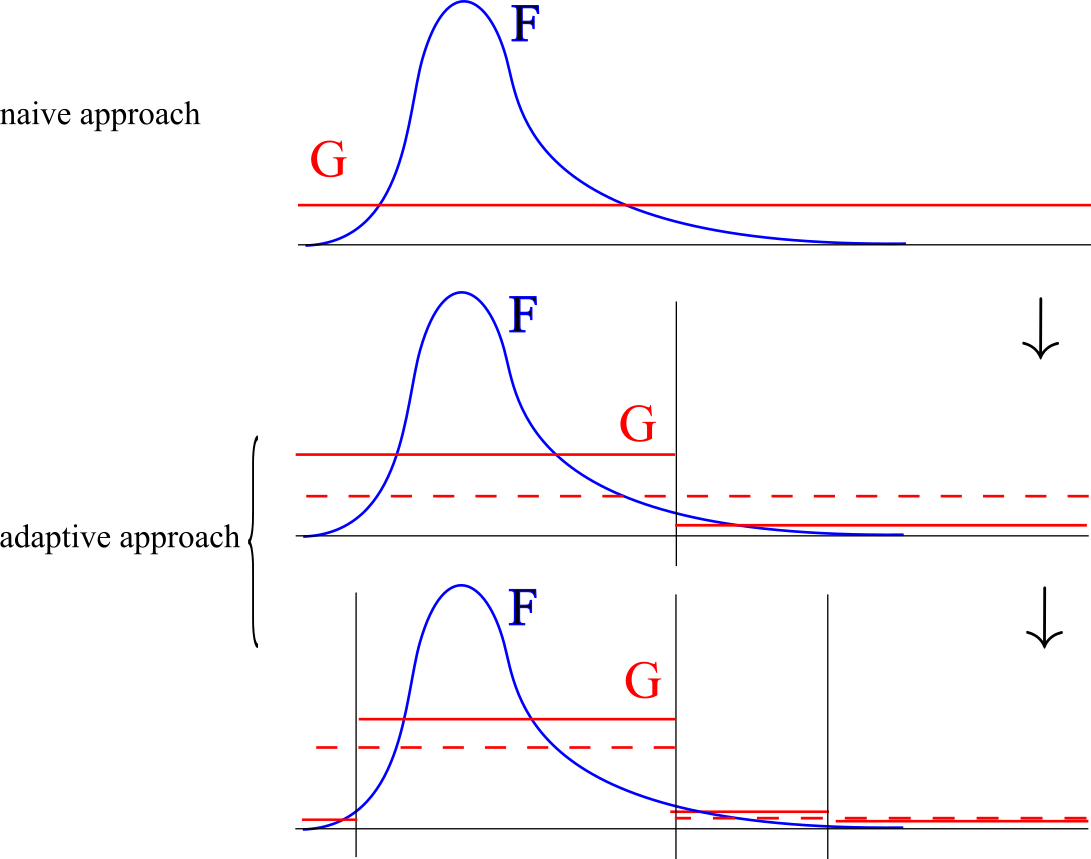
\includegraphics[width=0.8\linewidth]{fig_source/ocrf_fig/outlier_density.png}
  \caption{Outliers assumed distribution $G$ in the naive and adaptive approach.  In the naive approach, $G$ does not depends on the tree and is constant on the input space. In the adaptive approach the distribution depends on the inlier distribution $F$ through the tree. The outliers density is constant and equal to the average of $F$ on each node before splitting it.
%In the case of more than one tree, the resulting outlier distribution is then the average of such tree-specific densities.
}
  \label{ocrf:fig:outlier_density}
\end{figure}

\newcommand{\pointSampled}[1]{
    \coordinate (A) at (#1);
    \draw[fill=black] (A) circle (0.03cm);
}


\pgfmathsetseed{7}
\begin{figure}
\center
\begin{tikzpicture}[scale=1,declare function={
    %%cauchy distrib
    c1 = 6/10;
    c2 = 4/10;
    seuil = c1/(c1+c2);
    a1 = 0.1;
    a2 = 0.2;
    x01 = 0.8;
    x02 = 2.9;
    cauchyMass1(\x) = c1*a1/( pi*( pow(a1,2) + pow((\x-x01),2) ));
    cauchyMass2(\x) = c2*a2/( pi*( pow(a2,2) + pow((\x-x02),2) ));
      cauchyRepFuncInv1(\x) = a1*tan( 3.142*(\x-0.5) r) + x01;
      cauchyRepFuncInv2(\x) = a2*tan( 3.142*(\x-0.5) r) + x02;
      indicatorFunction(\x) = exp(-pow(\x-3,2)/6);
      %%params
      firstVerticalSplitX = 1;
      lastVerticalSplitX = 5.7;
      verticalDashedSplitX = 2.3;
      verticalSplitX = 4;
      lowHorizontalDashedSplitY = 4.5;
      highHorizontalDashedSplitY = 5.5;
      coeffHomothety = 3.8;
      homothetyBone = -1.7;
      homothetyBtwo = -14;
    },
]
  \definecolor{niceblue}{rgb}{0.4,0.4,0.9}
    \definecolor{blue2}{rgb}{0.9,1,1}

    %%% draw area
    \clip (-0.03,0.5) rectangle (13.8,6.8);

    %%% TOP RECTANGLES
    \draw[thick] (0,3.4) rectangle (6.5,6.7);
    \draw[thick] (7,3.4) rectangle (13.5,6.7);
    \node at (0.25,3.8) {$\mathcal{X}$};
    \node at (7.25,3.8) {$\mathcal{X}_t$};
    \node[color=niceblue] at (verticalSplitX+0.3,lowHorizontalDashedSplitY-0.2) {$\mathcal{X}_t$};


    %%%%%%%%%%%%%%%%%% LEFT PART
    %%% points sampling
  \foreach \x in {1,2,...,350}{
    \pgfmathsetmacro{\seuil}{c1/(c1+c2)}
    \pgfmathsetmacro{\aleatorio}{rnd}
    \pgfmathsetmacro{\rndCauchy}{\aleatorio>seuil ? 0 : 1 }
    \pgfmathsetmacro{\abscissePoint}{\rndCauchy*cauchyRepFuncInv1(rand) + (1-\rndCauchy)*cauchyRepFuncInv2(rand)}
    \pgfmathsetmacro{\ordinatePoint}{\rndCauchy*(1.5*rand+5) + (1-\rndCauchy)*(rand*0.4+5)}
    \pgfmathsetmacro{\abscissePointFiltered}{ \abscissePoint>6.6 ? -10 : \abscissePoint }
    \pointSampled{\abscissePointFiltered,\ordinatePoint}
    \pgfmathsetmacro{\rightEnough}{\abscissePoint>verticalDashedSplitX ? true : false }
    \pgfmathsetmacro{\leftEnough}{\abscissePoint<verticalSplitX ? true : false }
    \pgfmathsetmacro{\highEnough}{\ordinatePoint>lowHorizontalDashedSplitY ? true : false}
    \pgfmathsetmacro{\lowEnough}{\ordinatePoint<highHorizontalDashedSplitY ? true : false}
    \pgfmathsetmacro{\newAbscisse}{\rightEnough && \leftEnough && \highEnough && \lowEnough ? \abscissePoint*coeffHomothety + homothetyBone : -10  }
    \pointSampled{\newAbscisse,\ordinatePoint*coeffHomothety + homothetyBtwo}
  }


  %% curve
 \fill [blue2, domain=0.1:6.33, variable=\x]
      (0.1, 1)
      -- plot[samples=200,smooth] ({\x},{cauchyMass1(\x) + cauchyMass2(\x) +1} )
      -- (6.33, 1)
      -- cycle;
  \draw [domain=0.1:6.33, scale=1, color=niceblue, line width=1pt, fill=blue2] plot[samples=200,smooth] (\x,{cauchyMass1(\x) + cauchyMass2(\x) +1});
  %% axis
  \draw[->,>=latex] (0.1,1) to (0.1,3.2);
  \draw[->,>=latex] (0.1,1) to (6.5,1);

  %% splits
  \draw (firstVerticalSplitX,0.9) -- (firstVerticalSplitX,6.7); % gamma=10
  \draw (verticalSplitX,0.9) -- (verticalSplitX,6.7); % gamma=1
  %\draw (lastVerticalSplitX,0.9) -- (lastVerticalSplitX,6.7); % gamma=0.1
  %\node[below] at (firstVerticalSplitX,1){\footnotesize $\gamma=10$};
  %\node[below] at (verticalSplitX,1){\footnotesize $\gamma=1$};
  %\node[below] at (lastVerticalSplitX+0.5,1){\footnotesize $\gamma=0.1$};

  \draw (verticalDashedSplitX,0.9) -- (verticalDashedSplitX,6.7);
  \draw (0,lowHorizontalDashedSplitY) -- (6.5,lowHorizontalDashedSplitY);
  \draw (0,highHorizontalDashedSplitY) -- (6.5,highHorizontalDashedSplitY);

  %% ZOOM
  \draw[very thick, color=niceblue] (verticalDashedSplitX,lowHorizontalDashedSplitY) rectangle (verticalSplitX,highHorizontalDashedSplitY);
  \draw[very thick, dashed, color=niceblue,->,>=latex] (verticalDashedSplitX,highHorizontalDashedSplitY) -- (7,6.7);
  \draw[very thick, dashed, color=niceblue,->,>=latex] (verticalDashedSplitX,lowHorizontalDashedSplitY) -- (7,3.4);


  %%%%%%%%%%%%%%%%%% RIGHT PART second curve
  \fill [blue2, domain=7.1:13.53, variable=\x]
      (7.1, 1)
      -- plot[samples=200,smooth] ({\x},{ indicatorFunction((\x-7)/5)*coeffHomothety*1.5*cauchyMass2((\x-homothetyBone)/coeffHomothety)  +1 } )
      -- (13.53, 1)
      -- cycle;
  \draw[->,>=latex] (7.1,1) to (7.1,3.2);
  \draw[->,>=latex] (7.1,1) to (13.7,1);
  \draw [domain=7.1:13.53, scale=1, color=niceblue, line width=1pt] plot[samples=200,smooth] (\x,{ indicatorFunction((\x-7)/5)*1.5*coeffHomothety*cauchyMass2((\x-homothetyBone)/coeffHomothety)  +1} );

  %% splits
  \draw (verticalSplitX+7.25,0.9) -- (verticalSplitX+7.25,6.7); % gamma=1
  \draw (13.36,0.9) -- (13.36,6.7); % gammat
  \node[below] (gammaone) at (verticalSplitX+7.25,1){\footnotesize $\gamma=1$};
  \node[below] (gammat) at (13.36,1){\footnotesize $\gamma_t \simeq 0$};
  \draw[dashed] (7.1,1.23) -- (verticalSplitX+7.25,1.23);
  \node[right] at (6.65,1.35){\footnotesize $t_{\gamma}$};

  \draw[->,>=latex, very thick] (13.3,1.75) to (verticalSplitX+7.3,1.75);
  \node at (verticalSplitX+8.4,2)  {\textbf{adaptivity}};

\end{tikzpicture}
\caption{ The left part of this figure represents
the dataset under study and the underlying density.
After some splits on this initial node $\mathcal{X}$,
let us consider the node $\mathcal{X}_t$ illustrated in the right part of this figure:
without the proposed adaptive approach, the class ratio
$\gamma_t$ becomes too small
and leads to poor splits %(normal data are condensed on a very small volume)
(all the data are in the `normal side' of the split, which thus does not discriminate at all).
Contrariwise, setting $\gamma$ to one, \textit{i.e.} using our adaptative approach,
is far preferable.
Note that a given $\gamma$ corresponds to a level set $t_{\gamma}$.}
\label{ocrf:fig:split_alpha}

\end{figure}



\subsection{Prediction: a majority vote with one single candidate?}
\label{ocrf:sec:prediction}
 Now that RFs can be grown in the one-class setting using our one-class splitting criterion, the forest has to return a prediction adapted to this framework.
 In other words we also need to extend the concept of majority vote.
%
Most usual one-class (or more generally anomaly detection) algorithms actually provide more than just a level-set estimate or a predicted label for any new observation, abnormal vs. normal. Instead, they return a real valued function, termed \textit{scoring function}, defining a pre-order/ranking on the input space. Such a function $s: \mathbb{R}^d \to \mathbb{R}$ permits to rank any observations according to their supposed `degree of abnormality'. Thresholding it provides level-set estimates, as well as a decision rule that splits the input space into `normal' and `abnormal' regions.
%
%We thus adapt the majority vote to the one-class setting by defining the scoring function of a forest.
%
%We propose three natural scoring functions of a forest.
The scoring function $s(x)$ we use is the one defined in \cite{Liu2008}. It is a decreasing function of the average depth of the leaves containing $x$ in the forest, `if the trees were fully grown': an average term is added to each node containing more than one sample, say containing $N$ samples. This term $c(N)$ is the average depth of an extremely randomized tree \citep{Geurts2006} (\ie~built without minimizing any criterion, by randomly choosing one feature and one uniform value over this feature to split on) on $N$ samples. Formally,
\begin{align}
\label{ocrf:eq:scoring3}
\log_2 s(x) = -\left(\sum_{t \text{~leaves}} \mathds{1}_{\{ x \in t \}} d_t + c(n_t)\right) ~/~ c(n),
\end{align}
where $d_t$ is the depth of node $t$, and $c(n) = 2H(n - 1) - 2(n - 1)/n$, $H(i)$ being the harmonic number.
%
\begin{remark}[{\sc Alternative Scoring Functions}]
Although we use the scoring function defined in \eqref{ocrf:eq:scoring3} because of its established high performance \citep{Liu2008}, other scoring functions can be defined.
%\textbf{Score 1- Stepwise density estimate.}
A natural idea to adapt the majority vote to the one-class setting is to change the single vote of a leaf node $t$ into the fraction $\frac{n_t}{\leb(\mathcal{X}_t)}$, the forest output being the average of the latter quantity over the forest,
% \begin{align}
% \label{ocrf:eq:scoring1}
$s(x) = \sum_{t \text{~leaves}} \mathds{1}_{\{ x \in t \}} \frac{n_t}{\leb(\mathcal{X}_t)}.$
% \end{align}
In such a case, each tree of the forest yields a piece-wise density estimate, on its induced partition. % However, we are only interested in the order induced by this density estimate, and if the average of density estimates should be a good density estimate, this does not remains true for the average of order: in general, the average of scoring functions is not a good scoring function.
The output produced by the forest is then a \emph{step-wise density estimate}.
% , potentially good, but which is not (according to our experiments) as good as \eqref{ocrf:eq:scoring} as a scoring function. In other words, this density estimate is not accurate in estimating the support (or large level-sets) of the distribution.
% One possible explanation is that while averaging density estimate yields generally good density estimate, this is not necessary true when averaging orders/rankings. To see this, considering two scoring functions $s_1$ and $s_2$, $(s_1 + s_2)/2$ correspond to a different ranking than $(2s_1 + s_2)/2$, while $2s_1$ and $s_1$ correspond to the same ranking.
% %Besides, estimating a support using the support of a density average overestimate it, because it consists of the union of all the supports involved.
% In other terms, the average of scoring functions is not necessary a good scoring function.
% \end{remark}
%
%\textbf{Score 2- Local density of a typical cell.}
We could also think about the \emph{local density of a typical cell}.
For each point $x$ of the input space, it returns the average number of observations in the leaves containing $x$, divided by the average volume of such leaves.
The output of OneClassRF is then the scoring function
% \begin{align}
% \label{ocrf:eq:scoring2}
$s(x) = \big(\sum_{t \text{~leaves}} \mathds{1}_{\{ x \in t \}} n_t\big) \big(\sum_{t \text{~leaves}} \mathds{1}_{\{ x \in t \}} \leb(\mathcal{X}_t)\big)^{-1} ,$
% \end{align}
where the sums are over each leave of each tree in the forest.
This score can be interpreted as the local density of a `typical' cell (typical among those usually containing $x$).
%
%Instead of $\frac{n_t}{\leb(\mathcal{X}_t)}$, we could have consider for a leaf node $t_L$ with parent node $t$, the maximum between $n_{t_L}$ and $n_t'\lambda_L$ or the fraction  $\frac{n_{t_L}}{n_t'\lambda_L}$ which is a more natural adaptation of the majority vote. However, the latter quantity is equal to $\frac{n_{t_L}}{\leb(\Omega_{t_L})} / \frac{n_t'}{\leb(\Omega_t)}$, the rapport between the density of the leaf and the density of the parent node.
\end{remark}



\subsection{OneClassRF: a Generic One-Class Random Forest algorithm}
Let us summarize our One Class Random Forest algorithm, based on generic RFs \citep{Breiman2001}. It has $6$ parameters:
$max\_samples$, $max\_features\_tree$, $max\_features\_node$, $\gamma$, $max\_depth$, $n\_trees$.

Each tree is classically grown on a random subset of both the input samples and the input features \citep{Ho1998, Panov2007}.
This random subset is a sub-sample of size $max\_samples$, with $max\_features\_tree$ variables chosen at random without replacement (replacement is only done after the tree is grown). The tree is built by minimizing \eqref{ocrf:oc_proxy_ad2} for each split, using parameter $\gamma$ (recall that $n_t' := \gamma n_t$), until the maximal depth $max\_depth$ is achieved.
% define a large number of geometric features and search over a random selection
% of these for the best split at each node
Minimizing \eqref{ocrf:oc_proxy_ad2} is done as introduced in \cite{Amit1997}, defining a large number $max\_features\_node$ of geometric features and searching over a random selection of these for the best split at each node.
%
The forest is composed of a number $n\_trees$ of trees. The predicted score of a point $x$ is given by $s(x)$, the $s$'s being defined in Section~\ref{ocrf:sec:prediction}.
%SH (copier en suppl mat) As an illustration, Figure~\ref{ocrf:fig:oneclassrf} represents the level set of the scoring function produced by OneClassRF, with only one tree ($n\_trees$$=1$) of maximal depth $max\_depth$=4, without sub-sampling, and using the Gini-based one-class splitting criterion with $\gamma=1$.
% Remarks on the underlying level-set estimation, alternative stopping criteria and variable importances are available in supplementary material.



Figure~\ref{ocrf:fig:oneclassrf} represents the level set of the scoring function produced by OneClassRF, with only one tree ($n\_trees$$=1$) of maximal depth $max\_depth$=4, without sub-sampling, and using the Gini-based one-class splitting criterion with $\gamma=1$.
\begin{figure}[ht]
  \centering
  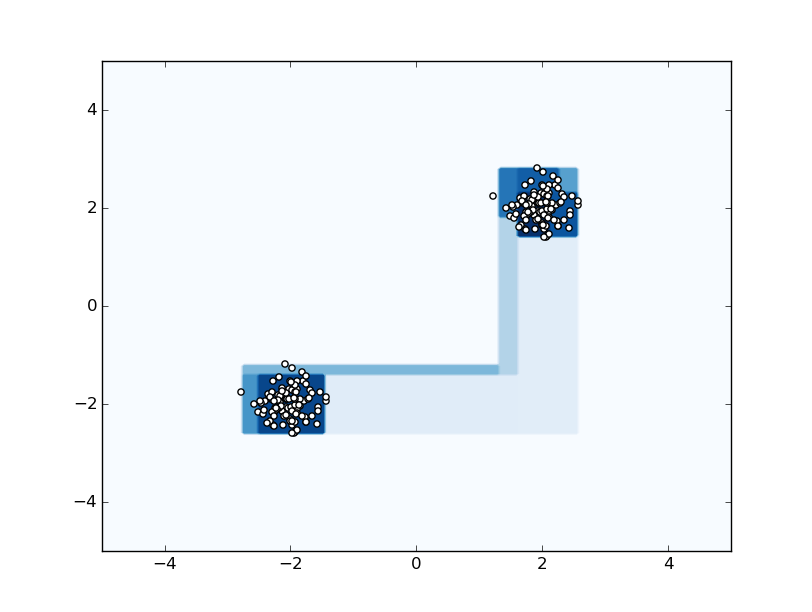
\includegraphics[width=0.5\linewidth]{fig_source/ocrf_fig/oneclassrf.png}
  \caption{OneClassRF with one tree: level-sets of the scoring function}
  \label{ocrf:fig:oneclassrf}
\end{figure}


% \begin{remark}({\sc Underlying Level-Set estimation})
% As mentionned above, the link between $\gamma$ and the level of the level-set estimate induced by the split is difficult to exhibit, as well as how it repercutes into the level of the global level-set estimate.
% Intuitively, $\gamma$ plays the same role as parameter $\nu$ for the OCSVM in its $\nu$-soft margin formulation.
% OCSVM also returns a scoring function (inducing an infinite number of level-sets), but which seeks to be optimal for estimating a particular level-set (corresponding to a particular thresholding of the scoring function) whose level can explicitely be controlled by $\nu$.
% However, we are not able to derive an explicit relation, as it exists for the OCSVM, between the targeted level set and $\gamma$. Note that this does not mean that we are not able to estimate any arbitrary level-set. It only means that we do not know for which level, the scoring function outputed by OneClassRF originally seeks to be optimal.
% \end{remark}


\begin{remark}({\sc Interpretation of $\gamma$})
\label{ocrf:rk:gamma}
In order for the splitting criterion \eqref{ocrf:oc_proxy_ad2} to perform well, $n_t'$ is expected to be of the same order of magnitude as the number of normal observations $n_t$. If $\gamma = n_t'/n_t \ll 1$, the split puts every normal data on the same side, even the ones which are far in the tail of the distribution, thus widely over-estimating the support of normal data. If $\gamma >> 1$, the opposite effect happens, yielding an estimate of a $t$-level set with $t$ not close enough to $0$.
Figure~\ref{ocrf:fig:split_alpha}
 illustrates the splitting criterion when $\gamma$ varies. It clearly shows that there is a link between parameter $\gamma$ and the level $t_\gamma$ of the induced level-set estimate. But from the theory, an explicit relation between $\gamma$ and $t_\gamma$ is hard to derive. By default we set $\gamma$ to $1$.
%
% The outlier sampling size $\gamma = n_t' / n_t$ is a parameter of the forest which controls at each split the level of the (local) estimated level-set (induced by the split), as illustrated in Figure~\ref{ocrf:fig:split_alpha}. %The more there is outliers, the higher the corresponding level. % the estimated level set/density support fit to the training data.
% The OneClassRF algorithm % takes as parameter the fraction $\alpha = n_t'/n_t$,
% fixed by default $\gamma=1$. %this parameter to $n_t'=n_t$.
One could object that in some situations, it is useful to randomize this parameter. For instance, in the case of a bi-modal distribution for the normal behavior, one split of the tree needs to separate two clusters, in order for the level set estimate to distinguish between the two modes. As illustrated in Figure~\ref{ocrf:fig:split_alpha_2}
, it can only occur if $n_t'$ is large with respect to $n_t$ ($\gamma >> 1$). However, the randomization of $\gamma$ is somehow included in the randomization of each tree, thanks to the sub-sampling inherent to RFs.
%
Moreover, small clusters tend to vanish when the sub-sample size is sufficiently small: a small sub-sampling size is used in \cite{Liu2008} to isolate outliers even when they form clusters.
\end{remark}





\pgfmathsetseed{7}
\begin{figure}
\center
\begin{tikzpicture}[scale=1,declare function={
    %%cauchy distrib
    c1 = 6/10;
    c2 = 4/10;
    seuil = c1/(c1+c2);
    a1 = 0.1;
    a2 = 0.2;
    x01 = 0.8;
    x02 = 2.9;
    cauchyMass1(\x) = c1*a1/( pi*( pow(a1,2) + pow((\x-x01),2) ));
    cauchyMass2(\x) = c2*a2/( pi*( pow(a2,2) + pow((\x-x02),2) ));
      cauchyRepFuncInv1(\x) = a1*tan( 3.142*(\x-0.5) r) + x01;
      cauchyRepFuncInv2(\x) = a2*tan( 3.142*(\x-0.5) r) + x02;
      indicatorFunction(\x) = exp(-pow(\x-3,2)/6);
      %%params
      firstVerticalSplitX = 1;
      lastVerticalSplitX = 5.7;
      verticalDashedSplitX = 2.3;
      verticalSplitX = 4;
      lowHorizontalDashedSplitY = 4.5;
      highHorizontalDashedSplitY = 5.5;
      coeffHomothety = 3.8;
      homothetyBone = -1.7;
      homothetyBtwo = -14;
    },
]
  \definecolor{niceblue}{rgb}{0.4,0.4,0.9}
    \definecolor{blue2}{rgb}{0.9,1,1}

    %%% draw area
    \clip (-0.03,0.5) rectangle (7,6.8);

    %%% TOP RECTANGLES
    \draw[thick] (0,3.4) rectangle (6.5,6.7);
    %\draw[thick] (7,3.4) rectangle (13.5,6.7);
    \node at (0.25,3.8) {$\mathcal{X}$};
    %\node at (7.25,3.8) {$\mathcal{X}_t$};
    %\node[color=niceblue] at (verticalSplitX+0.3,lowHorizontalDashedSplitY-0.2) {$\mathcal{X}_t$};


    %%%%%%%%%%%%%%%%%% LEFT PART
    %%% points sampling
  \foreach \x in {1,2,...,350}{
    \pgfmathsetmacro{\seuil}{c1/(c1+c2)}
    \pgfmathsetmacro{\aleatorio}{rnd}
    \pgfmathsetmacro{\rndCauchy}{\aleatorio>seuil ? 0 : 1 }
    \pgfmathsetmacro{\abscissePoint}{\rndCauchy*cauchyRepFuncInv1(rand) + (1-\rndCauchy)*cauchyRepFuncInv2(rand)}
    \pgfmathsetmacro{\ordinatePoint}{\rndCauchy*(1.5*rand+5) + (1-\rndCauchy)*(rand*0.4+5)}
    \pgfmathsetmacro{\abscissePointFiltered}{ \abscissePoint>6.6 ? -10 : \abscissePoint }
    \pointSampled{\abscissePointFiltered,\ordinatePoint}
    %\pgfmathsetmacro{\rightEnough}{\abscissePoint>verticalDashedSplitX ? true : false }
    %\pgfmathsetmacro{\leftEnough}{\abscissePoint<verticalSplitX ? true : false }
    %\pgfmathsetmacro{\highEnough}{\ordinatePoint>lowHorizontalDashedSplitY ? true : false}
    %\pgfmathsetmacro{\lowEnough}{\ordinatePoint<highHorizontalDashedSplitY ? true : false}
    %\pgfmathsetmacro{\newAbscisse}{\rightEnough && \leftEnough && \highEnough && \lowEnough ? \abscissePoint*coeffHomothety + homothetyBone : -10  }
    %\pointSampled{\newAbscisse,\ordinatePoint*coeffHomothety + homothetyBtwo}
  }


  %% curve
 \fill [blue2, domain=0.1:6.33, variable=\x]
      (0.1, 1)
      -- plot[samples=200,smooth] ({\x},{cauchyMass1(\x) + cauchyMass2(\x) +1} )
      -- (6.33, 1)
      -- cycle;
  \draw [domain=0.1:6.33, scale=1, color=niceblue, line width=1pt, fill=blue2] plot[samples=200,smooth] (\x,{cauchyMass1(\x) + cauchyMass2(\x) +1});
  %% axis
  \draw[->,>=latex] (0.1,1) to (0.1,3.2);
  \draw[->,>=latex] (0.1,1) to (6.5,1);

  %% splits
  \draw (firstVerticalSplitX,0.9) -- (firstVerticalSplitX,6.7); % gamma=10
  \draw (verticalSplitX,0.9) -- (verticalSplitX,6.7); % gamma=1
  \draw (lastVerticalSplitX,0.9) -- (lastVerticalSplitX,6.7); % gamma=0.1
  \node[below] at (firstVerticalSplitX,1){\footnotesize $\gamma=10$};
  \node[below] at (verticalSplitX,1){\footnotesize $\gamma=1$};
  \node[below] at (lastVerticalSplitX+0.5,1){\footnotesize $\gamma=0.1$};

  %\draw (verticalDashedSplitX,0.9) -- (verticalDashedSplitX,6.7);
  %\draw (0,lowHorizontalDashedSplitY) -- (6.5,lowHorizontalDashedSplitY);
  %\draw (0,highHorizontalDashedSplitY) -- (6.5,highHorizontalDashedSplitY);

  %% ZOOM
  %\draw[very thick, color=niceblue] (verticalDashedSplitX,lowHorizontalDashedSplitY) rectangle (verticalSplitX,highHorizontalDashedSplitY);
  %\draw[very thick, dashed, color=niceblue,->,>=latex] (verticalDashedSplitX,highHorizontalDashedSplitY) -- (7,6.7);
  %\draw[very thick, dashed, color=niceblue,->,>=latex] (verticalDashedSplitX,lowHorizontalDashedSplitY) -- (7,3.4);


  %%%%%%%%%%%%%%%%%% RIGHT PART second curve
  \vide{
  \fill [blue2, domain=7.1:13.53, variable=\x]
      (7.1, 1)
      -- plot[samples=200,smooth] ({\x},{ indicatorFunction((\x-7)/5)*coeffHomothety*1.5*cauchyMass2((\x-homothetyBone)/coeffHomothety)  +1 } )
      -- (13.53, 1)
      -- cycle;
  \draw[->,>=latex] (7.1,1) to (7.1,3.2);
  \draw[->,>=latex] (7.1,1) to (13.7,1);
  \draw [domain=7.1:13.53, scale=1, color=niceblue, line width=1pt] plot[samples=200,smooth] (\x,{ indicatorFunction((\x-7)/5)*1.5*coeffHomothety*cauchyMass2((\x-homothetyBone)/coeffHomothety)  +1} );

  %% splits
  \draw (verticalSplitX+7.25,0.9) -- (verticalSplitX+7.25,6.7); % gamma=1
  \draw (13.36,0.9) -- (13.36,6.7); % gammat
  \node[below] (gammaone) at (verticalSplitX+7.25,1){\footnotesize $\gamma=1$};
  \node[below] (gammat) at (13.36,1){\footnotesize $\gamma_t$};
  \draw[dashed] (7.1,1.23) -- (verticalSplitX+7.25,1.23);
  \node[right] at (6.65,1.35){\footnotesize $t_{\gamma}$};

  \draw[->,>=latex, very thick, color=niceblue] (13.3,1.3) to[bend right] (verticalSplitX+7.3,1.3);
  \node at (verticalSplitX+8.2,2)  {\color{niceblue} \textbf{adaptivity}};
  }
\end{tikzpicture}

\caption{Illustration of the standard splitting
criterion on two modes when the proportion $\gamma$ varies.}
\label{ocrf:fig:split_alpha_2}
\end{figure}







\begin{remark}({\sc Alternative Stopping Criteria})
Other stopping criteria than a maximal depth may be considered. We could stop splitting a node $t$ when it contains less than $n\_min$ observations, or when the quantity $n_t/\leb(\mathcal{X}_t)$ is large enough (all the points in the cell $\mathcal{X}_t$ are likely to be normal) or close enough to $0$ (all the points in the cell $\mathcal{X}_t$ are likely to be abnormal). These options are not discussed in this work.
\end{remark}

\begin{remark}({\sc Variable importances})
In the multi-class setting, \cite{Breiman2001} proposed to evaluate the importance of a feature $j \in \{1,\ldots d\}$ for prediction by %computing the following quantity. XXX
 adding up the weighted impurity decreases % $p(t) \Delta I(s_t, t)$
for all nodes $t$ where $X_j$ is used, averaged over all the trees. The analogue quantity can be computed with respect to the one-class impurity decrease proxy. % $I_{oc}(s_t, t)$.
In our one-class setting, this quantity represents the size of the tail of $X_j$, and can be interpreted as the capacity of feature $j$ to discriminate between normal/abnormal data.%, or the importance of feature $j$ to isolate anomalies
\end{remark}



%by \eqref{ocrf:eq:scoring1}, \eqref{ocrf:eq:scoring2} or \eqref{ocrf:eq:scoring3}.
% \paragraph{Description of the OneClassRF algorithm.}
% Now that we have exposed the one-class splitting rule to grow the trees, as well as the forest output replacing the majority vote, the one-class random forest algorithm promoted here is described as follows. %similar to Breiman's approach, see \cite{Breiman2001}.
% % Let us denote by \ttt{X} the input data.
% In its most generic version, it has five parameters, $max\_samples$, $max\_features$, $n\_estimators$, $max\_depth$ and $\gamma$.
% Each tree is classicaly grown on a random subset of both the input samples and the input variables, see~\cite{Ho1998, Panov2007}. This random subset is a sub-sample of size $max\_samples$, with $max\_features$ variables chosen at random without replacement (replacement is only done after the tree is grown). The tree is built by minimizing \eqref{ocrf:oc_proxy_ad2} at each step using parameter $\gamma$, until the maximal depth $max\_depth$ is achieved. The forest is composed of a number $n\_estimators$ of trees. The predicted score of a point $x$ is given by \eqref{ocrf:eq:scoring}, namely the average (over the trees) of $n_t/\leb(\mathcal{X}_t)$, where $t$ is the leaf node (of the tree considered) containing $x$.
% % \begin{algorithm}[OneClassRF.fit]~\\
% % \begin{pythoncode}
% % Inputs: X
% % Parameters: max_samples, max_features, n_estimators, max_depth
% % Output: A set of n_estimators trees.
% % \end{pythoncode}
% % \end{algorithm}



% \begin{remark}({\sc Extremely Randomized Trees})
%   In the case of extremely randomized trees (see \cite{Geurts2006}), namely trees grown totally randomly as used in Isolation Forest (\cite{Liu2008}), no splitting criterion is needed so that no impurity function is used. The one class version of the majority vote can still be used in this case, which yields a scoring function of the form $s(x) = \sum_t \mathds{1}_{\{\Omega_t \}} \frac{N_t}{\leb(\Omega_t)}$. XXX benchmark on this algo? (easy: iforest with score from OCSVM)
% \end{remark}
%XXX sklearn exemple with OneClassRF with different alpha








\section{Benchmarks}
%
\label{ocrf:sec:benchmark}
\begin{table}[ht]
\caption{Original Datasets characteristics}
\label{ocrf:table:data}
\centering
\footnotesize
%\tabcolsep=0.08cm
\resizebox{0.9\linewidth}{!} {
\begin{tabular}{lccll}
  \toprule
  Datasets        & nb of samples      & nb of features     & ~~~~~~~~~~~~~~~~~~~~~~~~~anomaly class      & ~                  \\ \midrule
  adult       & 48842              & 6                  &    class '$>50K$'                           &      (23.9\%)      \\
  annthyroid  & 7200               & 6                  &    classes $\neq$ 3                         &        (7.42\%)    \\
  arrhythmia  & 452                & 164                &    classes $\neq$ 1 (features 10-14 removed)&  (45.8\%)          \\
  forestcover & 286048             & 10                 &    class 4  (vs. class 2 )                  &           (0.96\%) \\
  http        & 567498             & 3                  &      attack                                 &    (0.39\%)        \\
  ionosphere  & 351                & 32                 &    bad                                      &       (35.9\%)     \\
  pendigits   & 10992              & 16                 &    class 4                                  &        (10.4\%)    \\
  pima        & 768                & 8                  &    pos (class 1)                            &        (34.9\%)    \\
  shuttle     & 85849              & 9                  &      classes $\neq$ 1 (class 4 removed)     &  (7.17\%)          \\
  smtp        & 95156              & 3                  &      attack                                 &    (0.03\%)        \\
  spambase    & 4601               & 57                 &    spam                                     &           (39.4\%) \\
  wilt        & 4839               & 5                  &    class 'w' (diseased trees)               &    (5.39\%)        \\
  \bottomrule
\end{tabular}
}
\end{table}
%
\begin{table}[!h]
\caption{Results for the novelty detection setting (semi-supervised framework).
%We compare various methods from the state-of-the-art (top line) to OneClassRF over different classical datasets (leftmost column).
The table reports AUC ROC and AUC PR scores (higher is better) for each algorithms.
%We use the set of hyper-parameters recommanded in the corresponding reference papers.
The training time of each algorithm has been limited (for each experiment among the 10 performed for each dataset) to 30 minutes,
where `NA' indicates that the algorithm could not finish training within the allowed time limit.
In average on all the datasets, our proposed algorithm `OneClassRF' achieves both best AUC ROC and AUC PR scores (with LSAD for AUC ROC). It also achieves the lowest cumulative training time.}
\label{ocrf:table:results-semisupervised}
\centering
%\scriptsize
\tabcolsep=0.1cm
\resizebox{\linewidth}{!} {
\begin{tabular}{ l  c@{\extracolsep{0.1cm}}c c@{\extracolsep{0.1cm}}c c@{\extracolsep{0.1cm}}c c@{\extracolsep{0.1cm}}c c@{\extracolsep{0.1cm}}c c@{\extracolsep{0.1cm}}c c@{\extracolsep{0.1cm}}c c@{\extracolsep{0.1cm}}c }
\toprule
%
Dataset & \multicolumn{2}{c }{OneClassRF} & \multicolumn{2}{c }{iForest} & \multicolumn{2}{c }{OCRF\small{sampl.}} & \multicolumn{2}{c }{OCSVM}& \multicolumn{2}{c }{LOF}& \multicolumn{2}{c }{Orca}& \multicolumn{2}{c }{LSAD}& \multicolumn{2}{c }{RFC}  \\%& parameters $(\epsilon, k)$\\
  \cmidrule{1-17}
~     & ROC &  PR & ROC &  PR & ROC & PR  & ROC & PR  & ROC & PR  &ROC  & PR  & ROC &  PR & ROC & PR  \\
adult        &        \textbf{0.665} & \textbf{0.278} & 0.661 & 0.227 & NA & NA & 0.638 & 0.201 & 0.615 & 0.188 & 0.606 & 0.218 &  0.647    & 0.258     & NA & NA \\
annthyroid   &        \textbf{0.936} & 0.468 & 0.913 & 0.456 & 0.918 & \textbf{0.532} & 0.706 & 0.242 & 0.832 & 0.446 & 0.587 & 0.181 &  0.810    & 0.327     & NA & NA \\
arrhythmia   &        0.684 & 0.510 & 0.763 & 0.492 & 0.639 & 0.249 & \textbf{0.922} & \textbf{0.639} & 0.761 & 0.473 & 0.720 & 0.466 &  0.778    & 0.514     & 0.716 & 0.299 \\
forestcover  &        0.968 & 0.457 & 0.863 & 0.046 & NA & NA & NA & NA & \textbf{0.990} & \textbf{0.795} & 0.946 & 0.558 &  0.952    & 0.166     & NA & NA \\
http         &        \textbf{0.999} & \textbf{0.838} & 0.994 & 0.197 & NA & NA & NA & NA & NA & NA & \textbf{0.999} & 0.812 &  0.981    & 0.537     & NA & NA \\
ionosphere   &        0.909 & 0.643 & 0.902 & 0.535 & 0.859 & 0.609 & 0.973 & 0.849 & 0.959 & 0.807 & 0.928 & \textbf{0.910} &  \textbf{0.978}    & 0.893     & 0.950 & 0.754 \\
pendigits    &        0.960 & 0.559 & 0.810 & 0.197 & 0.968 & 0.694 & 0.603 & 0.110 & 0.983 & 0.827 & \textbf{0.993} & \textbf{0.925} &  0.983    & 0.752     & NA & NA \\
pima         &        0.719 & 0.247 & 0.726 & 0.183 & \textbf{0.759} & \textbf{0.266} & 0.716 & 0.237 & 0.700 & 0.152 & 0.588 & 0.175 &  0.713    & 0.216     & 0.506 & 0.090 \\
shuttle      &        \textbf{0.999} & \textbf{0.998} & 0.996 & 0.973 & NA & NA & 0.992 & 0.924 & \textbf{0.999} & 0.995 & 0.890 & 0.782 &  0.996    & 0.956     & NA & NA \\
smtp         &        0.922 & 0.499 & 0.907 & 0.005 & NA & NA & 0.881 & \textbf{0.656} & \textbf{0.924} & 0.149 & 0.782 & 0.142 &  0.877    & 0.381     & NA & NA \\
spambase     &        \textbf{0.850} & 0.373 & 0.824 & 0.372 & 0.797 & \textbf{0.485} & 0.737 & 0.208 & 0.746 & 0.160 & 0.631 & 0.252 &  0.806    & 0.330     & 0.723 & 0.151 \\
wilt         &        0.593 & 0.070 & 0.491 & 0.045 & 0.442 & 0.038 & 0.323 & 0.036 & 0.697 & 0.092 & 0.441 & 0.030 &  0.677    & 0.074     & \textbf{0.896} & \textbf{0.631} \\
%internet_ads &     &       & & & & & & & &\\
\cmidrule{1-17}
average:    & \textbf{0.850} & \textbf{0.495} & 0.821 & 0.311 & 0.769 & 0.410 & 0.749 & 0.410 & 0.837 & 0.462 & 0.759 & 0.454 & \textbf{0.850}  & 0.450 &  0.758  & 0.385 \\
cum. train time: & \multicolumn{2}{c }{\textbf{61s}} & \multicolumn{2}{c }{68s} & \multicolumn{2}{c }{NA} & \multicolumn{2}{c }{NA}& \multicolumn{2}{c }{NA}& \multicolumn{2}{c }{2232s}& \multicolumn{2}{c }{73s}& \multicolumn{2}{c }{NA}  \\

  \bottomrule
\end{tabular}
}
\end{table}

In this section, we compare the OneClassRF algorithm described above to seven state-of-art anomaly detection algorithms:
the isolation forest algorithm \citep{Liu2008} (iForest), a one-class RFs algorithm based on sampling a second-class \citep{Desir12} (OCRFsampling), one class SVM \citep{Scholkopf2001} (OCSVM), local outlier factor \citep{Breunig2000LOF} (LOF), Orca \citep{Bay2003}, Least Squares Anomaly Detection \citep{Quinn2014} (LSAD), % EvOutSe (Evolutionary Outlier Search \cite{Aggarwal2001})
Random Forest Clustering \citep{Shi2012} (RFC).
%We have used default parameters for these algorithms, as detailed in supplementary material.

\subsection{Default parameters of OneClassRF.}
The default parameters taken for our algorithm are the followings.
%
$max\_samples$ is fixed to $20\%$ of the training sample size (with a minimum of $100$); $max\_features\_tree$ is fixed to $50\%$ of the total number of features with a minimum of $5$ (\ie~each tree is built on $50\%$ of the total number of features); $max\_features\_node$ is fixed to $5$; $\gamma$ is fixed to $1$ (see Remark~\ref{ocrf:rk:gamma}); $max\_depth$ is fixed to $\log_2$ (logarithm in base $2$) of the training sample size as in \cite{Liu2008}; $n\_trees$ is fixed to $100$ as in the previous reference; and parameter $s_i$ is set to $s_3$ as defined in \eqref{ocrf:eq:scoring3}.

\subsection{Hyper-Parameters of tested algorithms}
Overall we chose to train the different algorithms with their (default) hyper-parameters as seen
in their respective paper or author's implementation.

The \emph{OCSVM} algorithm uses default parameters: \verb+kernel='rbf'+, \verb+tol=1e-3+,
\verb+nu=0.5+, \verb+shrinking=True+, \verb+gamma=1/n_features+, where tol is the tolerance for stopping criterion.

The \emph{LOF} algorithm uses default parameters:
\verb+n_neighbors=5+, \verb+leaf_size=30+, \verb+metric='minkowski'+,
\verb+contamination=0.1+, \verb+algorithm='auto'+, where the algorithm parameters stipulates
how to compute the nearest neighbors (either ball-tree, kd-tree or brute-force).

The \emph{iForest} algorithm uses default parameters:
\verb+n_estimators=100+, \verb+max_samples=min(256, n_samples)+,
\verb+max_features=1+, \verb+bootstrap=false+, where bootstrap states whether samples are drawn with replacement.

The \emph{OCRFsampling} algorithm uses default parameters:
the number of dimensions for the Random Subspace Method \verb+krsm=-1+,
the number of features randomly selected at each node during the induction of the tree \verb+krfs=-1+,
\verb+n_tree=100+,
the factor controlling the extension of the outlier domain used for outlier generation according to the volume of the hyper-box surrounding the target data \verb+alpha=1.2+,
the factor controlling the number of outlier data generated according to the number of target data \verb+beta=10+,
whether outliers are generated from uniform distribution \verb+optimize=0+,
whether data outside target bounds are considered as outlier data \verb+rejectOutOfBounds=0+.

The \emph{Orca} algorithm uses default parameter \verb+k=5+ (number of nearest neighbors)
as well as \verb+N=n/8+ (how many anomalies are to be reported).
The last setting, set up in the empirical evaluation of iForest in \cite{Liu2012},
allows a better computation time without impacting Orca's performance.


The \emph{RFC} algorithm uses default parameters:
\verb+no.forests=25+, \verb+no.trees=3000+,
the Addcl1 Random Forest dissimilarity \verb+addcl1=T, addcl2=F+,
use the importance measure \verb+imp=T+,
the data generating process \verb+oob.prox1=T+,
the number of features sampled at each split \verb+mtry1=3+.

The \emph{LSAD} algorithm uses default parameters:
the maximum number of samples per kernel \verb+n_kernels_max=500+,
the center of each kernel (the center of the random sample subset by default) \verb+kernel_pos='None'+,
the kernel scale parameter (using the pairwise median trick by default)\verb+\gamma='None'+,
the regularization parameter \verb+rho=0.1+.

\subsection{Description of the datasets}
%
The characteristics of the twelve reference datasets considered here are summarized
in Table~\ref{ocrf:table:data}. They are all available on the UCI repository
\citep{Lichman2013} and the preprocessing is done in a classical way. %, excepting for the \emph{adult} dataset. For the latter, we considered the 6 continuous features.
We removed all non-continuous attributes as well as attributes taking less than $10$ different values.
%
The \emph{http} and \emph{smtp} datasets belong to the KDD Cup '99 dataset \citep{KDD99, Tavallaee2009}, which consist of a wide variety of hand-injected  attacks (anomalies) in a closed network (normal background). They are classically obtained as described in \cite{Yamanishi2000}. This two datasets are available on the \emph{scikit-learn} library \citep{sklearn2011}.
The \emph{shuttle} dataset is the fusion of the training and testing datasets available in the UCI repository. As in \cite{Liu2008}, we use instances from all different classes but class $4$.%, which yields an anomaly ratio (class 1) of $7.17\%$.
In the \emph{forestcover} data, the normal data are the instances from class~$2$ while instances from class $4$ are anomalies (as in \cite{Liu2008}). %, which yields an anomaly ratio of $0.9\%$.
The \emph{ionosphere} dataset differentiates `good' from `bad' radars, considered here as abnormal. A `good' radar shows evidence of some type of structure in the ionosphere. A `bad' radar does not, its signal passing through the ionosphere.
The \emph{spambase} dataset consists of spam or non-spam emails. The former constitute our anomaly class.
The \emph{annthyroid} medical dataset on hypothyroidism contains one normal class and two abnormal ones, which form our outliers.
The \emph{arrhythmia} dataset reflects the presence and absence (class $1$) of cardiac arrhythmia. The number of attributes being large considering the sample size, we removed attributes containing missing data.
The \emph{pendigits} dataset contains 10 classes corresponding to the digits from 0 to 9, examples being handwriting samples. As in \cite{Schubert2012}, the abnormal data are chosen to be those from class 4.
The \emph{pima} dataset consists of medical data on diabetes. Patients suffering from diabetes (normal class) were considered outliers.
The \emph{wild} dataset involves detecting diseased trees in Quickbird imagery. Diseased trees (class `w') is our abnormal class.
In the \emph{adult} dataset, the goal is to predict whether income exceeds \$ 50K/year based on census data. We only keep the 6 continuous attributes.
%Concerning the \emph{internet_ads} dataset, it contains characteristic of images, which may (class `ad', outlier) or not (class `nonad') be an advertisement.

\subsection{Results}
\pgfplotsset{minor grid style={very thick,black}}
\begin{figure}[ht]
\definecolor{ggreen}{rgb}{0.3,0.7,0.4}
\definecolor{ggreen2}{rgb}{0.4,0.8,0.5}
\definecolor{orange2}{rgb}{1,0.7,0}
\definecolor{violette}{rgb}{0.7,0.15,0.9}
\begin{tikzpicture}[scale=0.6,font=\Large]
\begin{axis}[ at={(0,0)},
              grid=minor,
              width=23cm, height=6cm,
              ybar=0pt,
              minor xtick={0.5,1.5,...,12.5},
              xmin=0.5, xmax=12.5,
              xticklabels={ , , , , , , , , , , , },
              ymin=0.58,
              ytick={0.6,0.7,...,1},
              ymax=1,
              ylabel={ROC AUC},
              legend entries={OneClassRF~~~~,iForest~~~~, OCRFsampling~~~~, OneClassSVM~~~~, LOF~~~~, Orca~~~~, LSAD~~~~, RFC},
legend style={at={(0.5,1.16)}, anchor=north,legend columns=-1}
              ]
\draw[dashed,black!30] (axis cs:0,0.6)--(axis cs:12.5,0.6);
\draw[dashed,black!30] (axis cs:0,0.7)--(axis cs:12.5,0.7);
\draw[dashed,black!30] (axis cs:0,0.8)--(axis cs:12.5,0.8);
\draw[dashed,black!30] (axis cs:0,0.9)--(axis cs:12.5,0.9);
\addplot+[bar width=4.5pt] plot table[x index=1, y index=3]{fig_source/ocrf_fig/results_semisupervised.txt};%OneClassRF
\addplot+[bar width=4.5pt] plot table[x index=1, y index=7]{fig_source/ocrf_fig/results_semisupervised.txt};%iForest
\addplot+[bar width=4.5pt] plot table[x index=1, y index=11]{fig_source/ocrf_fig/results_semisupervised.txt};%OCRFsampling
\addplot+[bar width=4.5pt] plot table[x index=1, y index=15]{fig_source/ocrf_fig/results_semisupervised.txt};%OneClassSVM
\addplot+[bar width=4.5pt, fill=ggreen!50, draw=ggreen] plot table[x index=1, y index=19]{fig_source/ocrf_fig/results_semisupervised.txt};%LOF
\addplot+[bar width=4.5pt, fill=violette!50, draw=violette] plot table[x index=1, y index=23]{fig_source/ocrf_fig/results_semisupervised.txt};%ORCA
\addplot+[bar width=4.5pt, fill=orange2!50, draw=orange2] plot table[x index=1, y index=27]{fig_source/ocrf_fig/results_semisupervised.txt};%LSAD
\addplot+[bar width=4.5pt,fill=white, draw=black!40] plot table[x index=1, y index=31]{fig_source/ocrf_fig/results_semisupervised.txt};%RFC
\end{axis}
\begin{axis}[ at={(0,-5cm)},
              grid=minor,
              width=23cm, height=6cm,
              ybar=0pt,
              minor xtick={0.5,1.5,...,12.5},
              xmin=0.5, xmax=12.5,
              xticklabels={ , , , , , , , , , , , },
              ymin=0.0,
              ytick={0.2,0.4,0.6,0.8,1},
              ymax=1,
              ylabel={PR AUC},
              %legend entries={OneClassRF~~~~,iForest~~~~, OCRFsampling~~~~, OneClassSVM~~~~, LOF~~~~, Orca~~~~, LSAD~~~~, RFC},
legend style={at={(0.5,1.16)}, anchor=north,legend columns=-1}
              ]
\draw[dashed,black!30] (axis cs:0,0.2)--(axis cs:12.5,0.2);
\draw[dashed,black!30] (axis cs:0,0.4)--(axis cs:12.5,0.4);
\draw[dashed,black!30] (axis cs:0,0.6)--(axis cs:12.5,0.6);
\draw[dashed,black!30] (axis cs:0,0.8)--(axis cs:12.5,0.8);
\addplot+[bar width=4.5pt] plot table[x index=1, y index=5]{fig_source/ocrf_fig/results_semisupervised.txt};%OneClassRF
\addplot+[bar width=4.5pt] plot table[x index=1, y index=9]{fig_source/ocrf_fig/results_semisupervised.txt};%iForest
\addplot+[bar width=4.5pt] plot table[x index=1, y index=13]{fig_source/ocrf_fig/results_semisupervised.txt};%OCRFsampling
\addplot+[bar width=4.5pt] plot table[x index=1, y index=17]{fig_source/ocrf_fig/results_semisupervised.txt};%OneClassSVM
\addplot+[bar width=4.5pt, fill=ggreen!50, draw=ggreen] plot table[x index=1, y index=21]{fig_source/ocrf_fig/results_semisupervised.txt};%LOF
\addplot+[bar width=4.5pt, fill=violette!50, draw=violette] plot table[x index=1, y index=25]{fig_source/ocrf_fig/results_unsupervised.txt};%ORCA
\addplot+[bar width=4.5pt, fill=orange2!50, draw=orange2] plot table[x index=1, y index=29]{fig_source/ocrf_fig/results_semisupervised.txt};%LSAD
\addplot+[bar width=4.5pt,fill=white, draw=black!40] plot table[x index=1, y index=33]{fig_source/ocrf_fig/results_semisupervised.txt};%RFC
\end{axis}
\begin{axis}[  at={(0,-13.4)},
              grid=minor,
              width=23cm,height=6cm,
              ybar=0pt,
              minor xtick={0.5,1.5,...,12.5},
              xmin=0.5, xmax=12.5,
              xtick={1,...,12},
              xticklabels={adult, annthyroid, arrhythmia, forestcover, http, ionosphere, pendigits, pima, shuttle, smtp, spambase, wilt},
              x tick label style={rotate=20,anchor=east},
              ymax=60, ymin=0,
              ytick={0,10,...,60},
              ylabel={Computation time (sec.)}
              ]
\draw[dashed,black!30] (axis cs:0,10)--(axis cs:12.5,10);
\draw[dashed,black!30] (axis cs:0,20)--(axis cs:12.5,20);
\draw[dashed,black!30] (axis cs:0,30)--(axis cs:12.5,30);
\draw[dashed,black!30] (axis cs:0,40)--(axis cs:12.5,40);
\draw[dashed,black!30] (axis cs:0,50)--(axis cs:12.5,50);
\addplot+[bar width=4.5pt] plot table[x index=1, y index=2]{fig_source/ocrf_fig/computationTime_semisupervised.txt};%OneClassRF
\addplot+[bar width=4.5pt] plot table[x index=1, y index=5]{fig_source/ocrf_fig/computationTime_semisupervised.txt};%iForest
\addplot+[bar width=4.5pt] plot table[x index=1, y index=8]{fig_source/ocrf_fig/computationTime_semisupervised.txt};%OCRFsampling
\addplot+[bar width=4.5pt] plot table[x index=1, y index=9]{fig_source/ocrf_fig/computationTime_semisupervised.txt};%OneClassSVM
\addplot+[bar width=4.5pt, fill=ggreen!50, draw=ggreen] plot table[x index=1, y index=12]{fig_source/ocrf_fig/computationTime_semisupervised.txt};%LOF
\addplot+[bar width=4.5pt, fill=violette!50, draw=violette] plot table[x index=1, y index=15]{fig_source/ocrf_fig/computationTime_semisupervised.txt};%ORCA
\addplot+[bar width=4.5pt, fill=orange2!50, draw=orange2] plot table[x index=1, y index=16]{fig_source/ocrf_fig/computationTime_semisupervised.txt};%LSAD
\addplot+[bar width=4.5pt,fill=white, draw=black!40] plot table[x index=1, y index=19]{fig_source/ocrf_fig/computationTime_semisupervised.txt};%RFC
\end{axis}
\end{tikzpicture}
\caption{Performances of the algorithms on each dataset in the novelty detection framework:
ROC AUCs are displayed on the top, Precision-Recall AUCs in the middle and training times\protect\footnotemark on the bottom, 
for each dataset and algorithm. The $x$-axis represents the datasets.}
\label{ocrf:figresultssemisupervised}
\end{figure}

\footnotetext{For OCRF, Orca and RFC, testing and training time cannot be isolated
because of algorithms implementation: for these algorithms, the sum of the training and testing times are displayed in Figure \ref{ocrf:figresultssemisupervised} and \ref{ocrf:figresultsunsupervised}.}

%
The experiments are performed in the novelty detection framework, also named
semi-supervised anomaly detection, where the training set consists of normal
data only. We simply removed anomalies from the training data.
%
%\subsection{Results}
%
For each algorithm, 10 experiments on random training and testing datasets are
performed, yielding averaged ROC and Precision-Recall curves whose AUC are
summarized in Table~\ref{ocrf:table:results-semisupervised}
(see the last section of this chapter to further insights on the benchmarks).
%
%Figures \ref{ocrf:figNoveltyAUCROC} and \ref{ocrf:figNoveltyCompTime}
%summarize the results. % from the novelty detection framework, whereas figures \ref{ocrf:figUnsupervAUCROC}, \ref{ocrf:figUnsupervAUCPR} and \ref{ocrf:figUnsupervCompTime} presents those from the unsupervised one.
% In the novelty detection settings,
It appears that OneClassRF has the best performance on five datasets
in terms of ROC AUCs, and is also the best in average.
%\footnote{Precision-Recall AUCs have also been computed and are
%available in the supplementary material.},
Computation times (training plus testing) of OneClassRF are also
very competitive. % (see supplementary material).
%In the unsupervised settings, OneClassRF and iForest have similar performances in terms of AUCs (ROC and PR), but OneClassRF still uses less computation time.
Figure~\ref{ocrf:figresultssemisupervised} shows that the amount of time
to train and test any dataset takes less than one minute with OneClassRF,
whereas some algorithms have far higher computation times (OCRFsampling,
OneClassSVM, LOF and Orca have computation times higher than 30 minutes in some
datasets). Our approach leads to results similar to quite new algorithms such as
iForest and LSDA.
%
%These results are surprising: iForest computation time should be lower since it randomly builds trees. The explaination is....
%
% T = np.array([[1.83, 1.19, np.NAN, 16.20, 7.03, 9.42, 1.05, np.NAN],
% [0.39, 0.19, 65.02, 0.54, 1.03, 0.66, 0.31, np.NAN],
% [0.36, 0.12, 9.30, 0.0, 0.04, 0.38, 0.01, 33.17],
% [19.97, 15.86, np.NAN, np.NAN, 59.56, 733.75, 6.18, np.NAN],
% [29.5, 42.25, np.NAN, np.NAN, np.NAN, 1368.83, 51.41, np.NAN],
% [0.36, 0.10, 2.47, 0.0, 0.03, 0.38, 0.0, 12.42],
% [0.67, 0.32, 458.94, 1.35, 1.66, 1.81, 0.42, np.NAN],
% [0.13, 0.10, 5.20, 0.0, 0.12, 0.26, 0.01, 18.12],
% [3.13, 3.87, np.NAN, 95.99, 20.39, 76.24, 7.42, np.NAN],
% [3.99, 3.51, np.NAN, 118.93, 12.11, 38.52, 5.98, np.NAN],
% [0.49, 0.21, 55.71, 0.22, 0.85, 1.49, 0.25, 593.87],
% [0.39, 0.16, 68.29, 0.14, 0.73, 0.46, 0.22, 752.19]])
% np.mean(T, axis=0)
% array([   5.10083333,    5.65666667,           nan,           nan,
%                  nan,  186.01666667,    6.105     ,           nan])



Experiments in an unsupervised framework (the training set is polluted by
abnormal data) have also been made. %In this case, the anomaly rate is arbitrarily bounded to $10\%$ max (before splitting data into training and testing sets).
The anomaly rate is arbitrarily bounded to $10\%$ max (before splitting data into training and testing sets).


\section{Theoretical jusification for the one-class splitting criterion}
\label{sec:ocrf:theory}
\subsection{Underlying model}
\label{ocrf:sec:model}
In order to generalize the two-class framework to the one-class one, we need to consider the population versions associated to empirical quantities \eqref{ocrf:eq:impurity_measure_decrease}, \eqref{ocrf:eq:gini} and \eqref{ocrf:eq:two_class_proxy}, as well as the underlying model assumption. The latter can be described as follows.

\textbf{Two-Class Model (n, $\boldsymbol{\alpha}$).}
We consider a random variable (\rv) $ X:\Omega \to \mathbb{R}^d$ \wrt~a probability space $(\Omega, \mathcal{F}, \mathbb{P})$.
The law of $X$ depends on another \rv~$y \in \{0,1\}$, verifying $\mathbb{P}(y=1)=1-\mathbb{P}(y=0)=\alpha$. We assume that conditionally on $y=0$, $ X$ follows a law $F$, and conditionally on $y=1$ a law $G$. To summarize:
\begin{align*}
 X ~|~ y=0 ~~\sim~~ F, &~~~~~~~~~~  \mathbb{P}(y=0)=1-\alpha, \\
 X ~|~ y=1 ~~\sim~~ G, &~~~~~~~~~~  \mathbb{P}(y=1)=\alpha.
\end{align*}
Then, considering  $p(t_L | t) = \mathbb{P}( X\in \mathcal{X}_{t_L} |  X\in \mathcal{X}_t)$,  $p(t_R | t) = \mathbb{P}( X\in \mathcal{X}_{t_R} |  X\in \mathcal{X}_t)$, the probabilistic version of \eqref{ocrf:eq:impurity_measure_decrease} is
\begin{align}
\label{ocrf:eq:impurity_measure_decrease_theo}
\Delta i^{theo}(t, t_L, t_R) ~~=~~ i^{theo}(t) ~-~  p(t_L | t)~ i^{theo}(t_L) ~-~  p(t_R | t)~ i^{theo}(t_R),
\end{align}
for instance using the Gini index $i^{theo} = i_G^{theo}$,
\begin{align}
\label{ocrf:eq:gini_theo}
  i_G^{theo}(t) ~~=~~ 2 \mathbb{P}(y=0 |  X \in \mathcal{X}_t) \cdot \mathbb{P}(y=1 |  X \in \mathcal{X}_t)
 ~~=~~ \frac{\mathbb{P}(X \in \mathcal{X}_t,~ y = 0) \cdot \mathbb{P}(X \in \mathcal{X}_t,~ y = 1) }{\mathbb{P}(X \in \mathcal{X}_t)^2}
\end{align}
% ~~=~~ \frac{(1-\alpha) \int_{\mathcal{X}_t}f ~~~ \alpha \int_{\mathcal{X}_t}g }{\left((1-\alpha) \int_{\mathcal{X}_t}f + \alpha \int_{\mathcal{X}_t}g\right)^2}
which is the population version of \eqref{ocrf:eq:gini}.
Indeed,
when observing $n$ \iid~realizations $( X_1, y_1),\ldots, ( X_n, y_n)$ of $( X,y)$, replacing probabilities by their empirical version amounts to replacing $\mathbb{P}(X \in \mathcal{X}_t,~ y = 0)$ by $n_t / n$, $\mathbb{P}(X \in \mathcal{X}_t,~ y = 1)$ by $n_t'/n$ and $\mathbb{P}(X \in \mathcal{X}_t)$ by $(n_t + n_t')/n$ with $n_t = \text{card}\{i,~X_i\in \mathcal{X}_t, y_i=0 \}$ and $n_t' = \text{card}\{i,~X_i\in \mathcal{X}_t, y_i=1 \}$, thus recovering \eqref{ocrf:eq:gini}.

\textbf{One-Class-Model ($n$, $\boldsymbol{\alpha}$).}
The one-class framework can be modeled as follows. Among the $n$ \iid~observations, we only observe those with $y=0$ (the normal behavior), namely $N$ realizations of $( X ~|~ y=0)$, where $N$ is itself a realization of a \rv~$\mb N$ of law $\mb N \sim \text{Bin}\big(n, (1-\alpha)\big)$. Here and hereafter, $\text{Bin}(n, p)$ denotes the binomial distribution with parameters $(n, p)$. As outliers are not observed, it is natural to assume that $G$ follows a uniform distribution on the hyper-rectangle $\mathcal{X}$ containing all the observations, so that $G$ has a constant density $g(x) \equiv 1 / \leb(\mathcal{X})$ on $\mathcal{X}$. %laisser une ligne car fin du model one class
Note that this assumption \emph{will be removed} in the adaptive approach described below (which aims at maintaining a non-negligible proportion of (hidden) outliers in every nodes).

Let us define $L_t=\leb(\mathcal{X}_t)/\leb(\mathcal{X})$. Then, $\mathbb{P}(X \in \mathcal{X}_t,~ y = 1)= \mathbb{P}(y = 1) \mathbb{P}(X \in \mathcal{X}_t|~ y = 1) = \alpha L_t $. Replacing in \eqref{ocrf:eq:gini_theo} the probability $\mathbb{P}(X \in \mathcal{X}_t, y=0)$ by its empirical version $n_t / n$, we then obtain the one-class empirical Gini index
\begin{align}
\label{ocrf:eq:gini_oc}
  i_G^{OC}(t) ~~=~~ \frac{n_t \alpha n L_t}{(n_t + \alpha n L_t)^2}.
\end{align}
In the following, we say that this one-class index is a \emph{semi-empirical} version of \eqref{ocrf:eq:gini_theo}, in the sense that it is obtained by considering empirical quantities for the (observed) normal behavior and population quantities for the (non-observed) abnormal behavior.
%
Now, maximizing the population version of the impurity decrease $\Delta i_G^{theo}(t, t_L, t_R)$ as defined in \eqref{ocrf:eq:impurity_measure_decrease_theo} is equivalent to minimizing
\begin{align}
\label{ocrf:theo_proxy}
 p(t_L | t)~ i_G^{theo}(t_L) ~+~  p(t_R | t)~ i_G^{theo}(t_R).
\end{align}
%Now, $p(t_L | t) = \left[\mathbb{P}(X\in \mathcal{X}_{t_L}~|~y=0) \mathbb{P}(y=0) + \mathbb{P}(X\in \mathcal{X}_{t_L}~|~y=1) \mathbb{P}(y=1)\right] / \mathbb{P}(X \in \mathcal{X}_t)$
Considering semi-empirical versions of $p(t_L | t)$ and $p(t_R | t)$, as for \eqref{ocrf:eq:gini_oc}, gives $p_n(t_L | t) = (n_{t_L} + \alpha n L_{t_L}) / (n_{t} + \alpha n L_{t})$ and $p_n(t_R | t) = (n_{t_R} + \alpha n L_{t_R}) / (n_{t} + \alpha n L_{t})$. Then, the semi-empirical version of \eqref{ocrf:theo_proxy} is
\begin{align}
\label{ocrf:oc_proxy1}
p_n(t_L | t)~ i_G^{OC}(t_L) ~+~  p_n(t_R | t)~ i_G^{OC}(t_R) = \frac{1}{(n_{t} + \alpha n L_{t})} \left(\frac{n_{t_L}\alpha n L_{t_L}}{n_{t_L} + \alpha n L_{t_L}} + \frac{n_{t_R}\alpha n L_{t_R}}{n_{t_R} + \alpha n L_{t_R}}\right)
\end{align}
where $ 1/(n_{t} + \alpha n L_{t})$ is constant when the split varies.
This means that finding the split minimizing \eqref{ocrf:oc_proxy1} is equivalent to finding the split minimizing
\begin{align}
\label{ocrf:oc_proxy2}
I_G^{OC}(t_L, t_R)= \frac{n_{t_L}\alpha n L_{t_L}}{n_{t_L} + \alpha n L_{t_L}} + \frac{n_{t_R}\alpha n L_{t_R}}{n_{t_R} + \alpha n L_{t_R}}.
\end{align}

\begin{remark} ({\sc Direct link with the two-class framework})
Note that the two-class proxy of the Gini impurity decrease \eqref{ocrf:tc_proxy} is easily recovered by replacing $\alpha n L_{t_L}$ (resp. $\alpha n L_{t_R}$) by $n'_{t_L}$ (resp. $n'_{t_R}$), the number of second class instances in $t_L$ (resp. in $t_R$). When generating $\alpha n$ of them uniformly on $\mathcal{X}$, $\alpha n L_{t}$ is the expectation of $n'_{t}$ .
\end{remark}


As detailed Section~\ref{sec:one-class-crit}, this approach suffers from the curse of dimensionality. 
We can summarize the problem as follows.
Consider $\gamma_t$ the ratio between the expected number of (hidden) outliers and the number of normal observations in node $t$, %, and have assumed that this ratio is negligible in nodes $t_L$ and $t_R$.
% \textbf{Problem 1.} Now, the curse of dimensionality appears in the following sense. In large dimension, $\alpha n L_{t}$ becomes very close to zero when going deeper in the tree (recall that $L_t = \leb(\mathcal{X}_t)/\leb(\mathcal{X})$, and the volume of $\mathcal{X}_t$ decreases). In addition, we typically grow trees on sub-samples of the input data, meaning that even the root node of the trees may be very small compared to the hyper-rectangle containing all the input data.
% %
% In other words, $\alpha n L_t$ is much smaller than $n_t$ for lots of nodes $t$ (in particular the leaves).
% Unfortunately, the Gini impurity is skew-sensitive \citep{Flach2003}. In other words, criterion \eqref{ocrf:oc_proxy2} almost does not penalize the volume for such nodes with $\alpha n L_t \ll n_t$.
%  This can also be seen when writing
% \begin{align}
% \label{ocrf:eq:I_with_gamma}
% I_G^{OC}(t_L, t_R) ~~=~~ \frac{\alpha n L_{t_L}}{1 + \gamma_{t_L}} + \frac{\alpha n L_{t_R}}{1 + \gamma_{t_R}} ~~\simeq~~ \alpha n L_{t_L} + \alpha n L_{t_R} ~~=~~ \alpha n L_{t},
% \end{align}
% $\alpha n L_{t}$ being constant when the split varies. We have used the notation %$\gamma_t$ is
\begin{align}
\label{ocrf:def:gamma_t}
\gamma_t := \frac{\alpha n L_t}{n_t}.
\end{align}
This class ratio is close to $0$ for lots of nodes $t$, which makes unable the Gini criterion to discriminate accurately between the (hidden) outliers and the inliers.
%
%\sim (n_{t_L}\alpha n L_{t_L}/n_{t_L} + n_{t_R}\alpha n L_{t_R}/n_{t_R}) = \alpha n L_{t}$$
%
% It turns out that criterion \eqref{ocrf:oc_proxy2} almost doesn't penalize the volume for such nodes with $\alpha n L_t \ll n_t$.
% This can be explained by the fact that the Gini impurity is skew-sensitive \cite{Flach2003} and also by writting the following equivalence of \eqref{ocrf:oc_proxy2} when $\alpha n L_{t} = (\alpha n L_{t_L} + \alpha n L_{t_R}) \to 0$:  $I_G^{OC}(t_L, t_R) \sim (n_{t_L}\alpha n L_{t_L}/n_{t_L} + n_{t_R}\alpha n L_{t_R}/n_{t_R}) = \alpha n L_{t}$, the last quantity being constant when the split varies.
%
Minimizing this criterion produces splits corresponding to $\gamma_t\simeq 0$ in Figure \ref{ocrf:fig:split_alpha}: one of the two child nodes, say $t_L$ contains almost all the data. 
%
%, as its volume is not sufficiently penalized (or equivalently $\alpha n L_{t_L}$ is negligible).
%and \ref{ocrf:fig:split_two_modes}. % (the $\gamma$ parameter represents a weight on the volume and will be formally introduced latter)

% To illustrate the fact that $\alpha n L_{t}$ becomes very close to zero in large dimension for lots of nodes $t$ (in particular the leaves), suppose for the sake of simplicity that the input space is $\mathcal{X} = [0,1]^d$. Suppose that we are looking for a rough precision of $1/2^3=0.125$ in each dimension, \ie~a unit cube precision of $2^{-3d}$.
% To achieve such a precision, we will typically need to use the splitting criterion on nodes/cells $t$ of volume of order $2^{-3d}$, namely with $L_t = 1/2^{3d}$.
% This means that $\alpha n$ should be of order $2^{3d}$ to have non-negligible $\alpha n L_{t}$, which is unreasonable for large $d$.

\subsection{Adaptive approach}

A solution is to remove the uniform assumption for the abnormal class.
The idea is to choose in an adaptive way (\wrt~the volume of $\mathcal{X}_t$) the number $\alpha n$, which can be interpreted as the number of (hidden) outliers. Recall that neither $n$ nor $\alpha$ is observed in the One-Class-Model($n$, $\alpha$). Doing so, we aim at avoiding $\alpha n L_t \ll n_t$ when $L_t$ is too small. Namely, with $\gamma_t$ defined in \eqref{ocrf:def:gamma_t}, we aim at avoiding $\gamma_t \simeq 0$ when $L_t \simeq 0$. The idea is to consider $\alpha(L_t)$ and $n(L_t)$ such that $\alpha(L_t) \to 1$, $n(L_t) \to \infty$ when $L_t \to 0$.
We then define the one-class adaptive proxy of the impurity decrease by
\begin{align}
\label{ocrf:oc_proxy_ad1}
I_G^{OC-ad}(t_L, t_R)= \frac{n_{t_L}\alpha(L_t) \cdot n(L_t) \cdot L_{t_L}}{n_{t_L} + \alpha(L_t) \cdot n(L_t) \cdot L_{t_L}} + \frac{n_{t_R}\alpha(L_t) \cdot n(L_t) \cdot L_{t_R}}{n_{t_R} + \alpha(L_t) \cdot n(L_t) \cdot L_{t_R}}.
\end{align}
In other words, instead of considering one general model One-Class-Model($n$, $\alpha$) defined in Section~\ref{ocrf:sec:model}, we adapt it to each node $t$, considering One-Class-Model($n(L_t)$, $\alpha(L_t)$) \emph{before searching the best split}. We still consider the $N$ normal observations as a realization of this model. When growing the tree, using One-Class-Model($n(L_t)$, $\alpha(L_t)$) as $L_t$ becomes close to zero allows to maintain a high expected proportion of outliers in the node to be split minimizing \eqref{ocrf:oc_proxy_ad1}.
Of course, constraints have to be imposed to ensure consistency between these models.
%
Recalling that the number $N$ of normal observations is a realization of $\mb N$ following a Binomial distribution with parameters $(n, 1-\alpha)$, a first natural constraint on $\big(n(L_t), \alpha(L_t)\big)$ is
\begin{align}
\label{ocrf:constraint1}
(1-\alpha)n = \big(1-\alpha(L_t)\big) \cdot n(L_t) \text{~~~~~for all~~} t,
\end{align}
so that the expectation of $\mb N$ remains unchanged. % when our new model depending on $t$ varies. %\ie~$\mathbb{E}(\mb N(L_t)) = \mathbb{E}(N) $ , %denoting $\mb N(L_t) \sim \text{Bin}(1-\alpha(L_t), n(L_t))$ .
%

\begin{remark}
In our adaptive model One-Class-Model($n(L_t)$, $\alpha(L_t)$) which varies when we grow the tree, let us denote by $\mb N(L_t) \sim \text{Bin}\big(n(L_t), 1-\alpha(L_t)\big)$ the \rv~ruling the number of normal data. The number of normal observations $N$ is still viewed as a realization of it. Note that the distribution of $\mb N(L_t)$ converges in distribution to $\mathcal{P}\big((1-\alpha)n\big)$ a Poisson distribution with parameter $(1-\alpha) n$ when $L_t \to 0$, while the distribution $\text{Bin}\big(n(L_t), \alpha(L_t)\big)$ of the \rv~$n(L_t) - \mb N(L_t)$ ruling the number of (hidden) outliers goes to infinity almost surely. In other words, the asymptotic model (when $L_t \to 0$) consists in assuming that the number of normal data $N$ we observed is a realization of $\mb N_\infty \sim \mathcal{P}\big((1-\alpha)n\big)$, and that an infinite number of outliers have been hidden.
\end{remark}


A second natural constraint on $\big(\alpha(L_t), n(L_t)\big)$
concerns on $\gamma_t$ defined in \eqref{ocrf:def:gamma_t},
%$\mathbb{P}(y = 1~|~X \in \mathcal{X}_t) = \alpha(L_t) n(L_t)  L_t / (n_t + \alpha(L_t) n(L_t)  L_t)$,
the ratio between the expected number of (hidden) outliers in node $t$ and the number of normal observations.
%, used to find the split by minimizing \eqref{ocrf:oc_proxy2}.
As explained in Section~\ref{sec:one-class-crit}, we do not want $\gamma_t$ to go to zero when $L_t$ does.
Let us say we want $\gamma_t$ to be constant for all node $t$, equal to $\gamma>0$. Typically, $\gamma=1$ so that there is as much expected uniform (hidden) outliers than normal data at each time we want to find the best split minimizing~\eqref{ocrf:oc_proxy_ad1}. Then the second constraint is % $n_t'/n(L_t)$, so that
\begin{align}
\label{ocrf:constraint2}
\alpha(L_t) \cdot n(L_t) \cdot L_t = \gamma_t n_t = \gamma n_t:=n_t'.
\end{align}
The quantity $n_t'$ can be interpreted as the expected number of (hidden) outliers in node $t$. The constant $\gamma$ is a parameter ruling the expected proportion of outliers in each node.
 % relies on $\mathbb{P}(X \in \mathcal{X}_t,~ y = 1) = \alpha(L_t)  L_t$, interpreted as the expected proportion of (unobserved) outliers in node $t$ we need to have before chosing the split by minimizing \eqref{ocrf:oc_proxy2}. Let say we want this probability to be equal to $n_t'/n(L_t)$, so that
% \begin{align}
% \label{ocrf:constraint2}
% \alpha(L_t)n(L_t)L_t = n_t'.
% \end{align}
%
Equations \eqref{ocrf:constraint1} and \eqref{ocrf:constraint2} allow to explicitly determine $\alpha(L_t)$ and $n(L_t)$: $\alpha(L_t) = n_t'/\big((1-\alpha)nL_t + n_t'\big)$ and $n(L_t) = \big((1-\alpha)nL_t + n_t'\big)/L_t$.
Regarding \eqref{ocrf:oc_proxy_ad1}, $\alpha(L_t) \cdot n(L_t) \cdot L_{t_L} = \frac{n_t'}{L_t} L_{t_L} = n_t'\leb(\mathcal{X}_{t_L})/ \leb(\mathcal{X}_{t})$ by \eqref{ocrf:constraint2} and $\alpha(L_t) \cdot n(L_t) \cdot L_{t_R}  = n_t'\leb(\mathcal{X}_{t_R})/\leb(\mathcal{X}_{t})$, so that
we recover equation~\eqref{ocrf:oc_proxy_ad2}.
% \begin{align}
% \label{ocrf:oc_proxy_ad2}
% I_G^{OC-ad}(t_L, t_R)= \frac{n_{t_L}n_t'\lambda_L}{n_{t_L} + n_t'\lambda_L} + \frac{n_{t_R}n_t'\lambda_R}{n_{t_R} + n_t'\lambda_R},
% \end{align}
% with $\lambda_L = \frac{\leb(\mathcal{X}_{t_L})}{\leb(\mathcal{X}_{t})}$ and $\lambda_R = \frac{\leb(\mathcal{X}_{t_R})}{\leb(\mathcal{X}_{t})}$.

% Minimization of the one-class Gini improvement proxy \eqref{ocrf:oc_proxy_ad2} is illustrated in Figure \ref{ocrf:fig:split_alpha}. %and \ref{ocrf:fig:split_two_modes}.
% Note that $n_t'\lambda_L$ (resp. $n_t'\lambda_R$) is the expectation of the number of uniform observations among $n_t'$ falling into the left (resp. right) node.

% Choosing the split minimizing $I_G^{OC-ad}(t_L, t_R)$ at each step of the tree building process, corresponds to generating $n_t'$ outliers each time the best split has to be chosen for node $t$, and then using the classical two-class Gini proxy \eqref{ocrf:tc_proxy}. The only difference is that $n_{t_L}'$ and $n_{t_R}'$ are replaced by their expectations $n_t'\lambda_{t_L}$ and $n_t'\lambda_{t_R}$ in our method. This attests the relevance of the above methodology.

% \begin{remark}({\sc By-product: Efficiently generating outliers})
% As a by-product, we obtain an efficient method to generate outliers tightly concentrated around the support of the normal distribution: it suffices to generate them as described above, recursively during the tree building process. Sampling $n_t'$ uniform points on $\mathcal{X}_t$, then using the latter to find the best split \wrt~\eqref{ocrf:tc_proxy}, and recommence on $\mathcal{X}_{t_L}$ and $\mathcal{X}_{t_R}$.
% \end{remark}

% Considering semi-empirical quantities (\ie~working with the limit behavior of uniformly generated outliers) implies that we loose some randomness % TODO DROUGUI: there where randomness before?
% in the tree building process, thus increasing the corelation between the trees of the forest.
% That is why we use a small sub-sampling size to build each tree, in the spirit of~\cite{Liu2008}. Growing each tree on a small sub-sample also allows to avoid randomizing the outlier number $n_t'$ at each step, see Remark~\ref{ocrf:rk:weight}.


% In pratice, the probability $\mathbb{P}(X \in \mathcal{X}_t,~ y = 1)=\alpha(L_t)L_t=n_t'/n(L_t)$ has to be of the same order than $\mathbb{P}_n(X \in \mathcal{X}_t,~ y = 0) = n_t /n(L_t)$, so that we set $n_t' = \beta n_t$ with $\beta \in (0,1)$ a parameter of the algorithm. (XXX $\beta$ = notre $\alpha$ dnas la version précedente)

% XXXXXXXXXXXXXXx
% %Suppose that the curse of dimensionality described above does not exist,
% Suppose that $n_t'$ outliers are generated, uniformly and independently on $\mathcal{X}_t$ the rectangular cell of a node $t$. After splitting node $t$, the expected number of outliers in the left node $t_L$ (resp. in the right node $t_R$) is $n_t' \frac{L_{t_L}}{L_{t}}$ (resp. $n_t'\frac{L_{t_R}}{L_{t}}$) where $L_{t}$ denotes the Lebesgue measure of node $t$.
% %
% Within this setup, the curse of dimensionality described in previous section can be interpreted as follows.


% \textbf{Problem 1.} After a few splits, if $n_t'$ is not unreasonably large beside the dimension of the input space, the actual number of outliers in a node will be negligeable, so that in the node/cells where the (non-uniform) normal distribution concentrates, the two classes are so highly unbalanced that the splitting criterion is useless.

% To illustrate this point, suppose for the sake of simplicity,
% that the input space is $[0,1]^d$, and that we are seeking a rough precision of $1/2^3=0.125$ in each dimension, \ie~a unit cube precision of $2^{-3d}$.
% %Assume that the normal observations concentrate
% To achieve such a precision, we will typically need to use the splitting criterion on node/cell (containing some normal observations) of volume slightly greater than $2^{-3d}$, say $2^{-3d +1}$.
% In average, this cell contains $n_t'/2^{3d}$ outliers.
% This means that $n_t'$ should be at least equal to $2^{3d}$ for expecting to have one in this cell, which is unreasonable for large $d$.

%split tends to be totally random (any split yields `pure' nodes, with a majority proportion of outliers).


%\parbox{13cm}{\center (uniform generated outliers are not represented)}

% \begin{minipage}{0.45\linewidth}
% \centering
% \includegraphics[width=\linewidth]{split_alpha.png}
% \captionof{figure}{Standard splitting criterion when the proportion $\gamma$ of generated outliers varies}
% \label{ocrf:fig:split_alpha}
% \end{minipage}\hfill
% \begin{minipage}{0.45\linewidth}
% \centering
% \includegraphics[width=\linewidth]{split_two_modes}
% \captionof{figure}{Standard splitting criterion on two modes when $\gamma$ varies}
% \label{ocrf:fig:split_two_modes}
% \end{minipage}



% Our solution to Problem 1. is to (do as if we) generate outliers locally, step by step, to maintain a reasonable number of them in cells containing normal data (empty cells does not need to be split). This is allowed by the following proposition.


% This proposition allows to generate outliers locally, node by node. When looking for the best split on node $t$, it suffices to generate an arbitrary number $n_t'$ of outliers in $\mathcal{X}_t$ and to find the split minimizing $I(t_L, t_R)$.
% Even more, we can avoid generating outliers, working directly with expectations, namely setting $n_{t_L}' = n_t' \lambda_L$ and $n_{t_R}' = n_t' \lambda_R$ where $\lambda_L = \frac{L_{t_L}}{L_t}$ (resp. $\lambda_R = \frac{L_{t_R}}{L_t}$) is the volume fraction of the left (resp. right) side node, for a chosen $n_t'$ (for instance $n_t'=n_t$). Replacing $n_{t_L}$ and $n_{t_R}$ by these values in the impurity improvement proxy \eqref{ocrf:eq:two_class_proxy} with the Gini index \eqref{ocrf:eq:gini} gives the following one-class Gini improvement proxy.
% %
% \begin{definition}({\sc One Class Gini improvement proxy}) As an analogue of the Gini impurity decrease proxy \eqref{ocrf:eq:two_class_proxy}, we define the one-class Gini improvement proxy by
% \begin{align}
% \label{ocrf:eq:one_class_gini_proxy}
% I_G(t_L, t_R) / 2 = \frac{n_{t_L} n_t' \lambda_L}{n_{t_L} + n_t' \lambda_L}
% + \frac{n_{t_R} n_t' \lambda_R}{n_{t_R} + n_t' \lambda_R} = \left( \frac{1}{n_{t_L}} + \frac{1}{n_t' \lambda_L} \right)^{-1} + \left( \frac{1}{n_{t_R}} + \frac{1}{n_t' \lambda_R} \right)^{-1},
% \end{align}
% where $n_t$ stands for the number of observations in node $t$, while $n_t'=\gamma n_t$ is a weight parameter on the outlyingness of the surrounding volume (it would be the number of generated outliers if we would be really generating them).
% \end{definition}



\section{Conclusion}
Through a natural adaptation of both (two-class) splitting criteria and majority vote, this chapter introduces a methodology to structurally extend RFs to the one-class setting.
%
Incidentally, our one-class splitting criteria correspond to the asymptotic behavior of an adaptive outliers generating methodology, so that consistency with two-class RFs seems respected.
%
Strong empirical performance attests the relevance of this methodology.

% % Reducing spacing in the bibliography
% % \let\oldbibliography\thebibliography
% % \renewcommand{\thebibliography}[1]{\oldbibliography{#1}
% % \setlength{\itemsep}{1pt}}

% {\small
% \bibliographystyle{plain}
% \bibliography{mvextrem}
% }


%\clearpage

\section{Further details on benchmarks and unsupervised results}


Recall that for each algorithm, 10 experiments on random training and testing datasets are performed. Averaged ROC and Precision-Recall curves AUC are summarized in Table~\ref{ocrf:table:results-semisupervised}.
%
For the experiments made in an unsupervised framework (meaning that the training set is polluted by abnormal data), the anomaly rate is arbitrarily bounded to $10\%$ max (before splitting data into training and testing sets).


%XXX TODO: description of the table


% M = np.array([[ 0.625, 0.161, 0.644, 0.234, np.NAN, np.NAN, 0.622, 0.179, 0.546 , 0.100   , 0.593 , 0.179   , 0.633 , 0.204       , np.NAN   , np.NAN],
% [ 0.842 , 0.226   , 0.820 , 0.310   , 0.992 , 0.869   , 0.688 , 0.193   , 0.731 , 0.188   , 0.561 , 0.132   , 0.762 , 0.246       , np.NAN   , np.NAN],
% [ 0.698 , 0.485   , 0.746 , 0.418   , 0.704 , 0.276   , 0.916 , 0.630   , 0.765 , 0.468   , 0.741 , 0.502   , 0.733 , 0.393       , 0.711 , 0.309],
% [ 0.845 , 0.044   , 0.882 , 0.062   , np.NAN   , np.NAN     , np.NAN , np.NAN   , 0.550 , 0.017   , 0.696 , 0.045   , 0.816 , 0.072       , np.NAN   , np.NAN],
% [ 0.984 , 0.120   , 0.999 , 0.685   , np.NAN   , np.NAN    , np.NAN , np.NAN   , np.NAN   , np.NAN     , 0.998 , 0.402   , 0.277 , 0.074       , np.NAN   , np.NAN],
% [ 0.903 , 0.508   , 0.888 , 0.545   , 0.879 , 0.664   , 0.956 , 0.813   , 0.956 , 0.789   , 0.929 , 0.917   , 0.915 , 0.773       , 0.943 , 0.725],
% [ 0.453 , 0.085   , 0.463 , 0.077   , 0.999 , 0.993   , 0.366 , 0.066   , 0.491 , 0.086   , 0.495 , 0.086   , 0.513 , 0.091       , np.NAN   , np.NAN],
% [ 0.708 , 0.229   , 0.743 , 0.205   , 0.790 , 0.296   , 0.706 , 0.226   , 0.670 , 0.137   , 0.585 , 0.170   , 0.686 , 0.190       , 0.505 , 0.091],
% [ 0.947 , 0.491   , 0.997 , 0.979   , np.NAN   , np.NAN     , 0.992 , 0.904   , 0.526 , 0.115   , 0.655 , 0.320   , 0.686 , 0.218       , np.NAN  , np.NAN],
% [ 0.916 , 0.400   , 0.902 , 0.005   , np.NAN   , np.NAN     , 0.881 , 0.372   , 0.909 , 0.053   , 0.824 , 0.236   , 0.888 , 0.398       , np.NAN   , np.NAN],
% [ 0.830 , 0.300   , 0.799 , 0.303   , 0.970 , 0.877   , 0.722 , 0.192   , 0.664 , 0.120   , 0.603 , 0.210   , 0.731 , 0.229       , 0.684 , 0.134],
% [ 0.520 , 0.053   , 0.443 , 0.044   , 0.966 , 0.554   , 0.316 , 0.036   , 0.627 , 0.069   , 0.441 , 0.029   , 0.530 , 0.053       , 0.876 , 0.472]])
% np.nanmean(M, axis=0)





%XXX TODO: description of the table
\begin{table}[h]
\caption{Results for the unsupervised setting}
\label{table:results-unsupervised}

\centering
%\scriptsize
\tabcolsep=0.1cm
\resizebox{\linewidth}{!} {
\begin{tabular}{ l  c@{\extracolsep{0.1cm}}c c@{\extracolsep{0.1cm}}c c@{\extracolsep{0.1cm}}c c@{\extracolsep{0.1cm}}c c@{\extracolsep{0.1cm}}c c@{\extracolsep{0.1cm}}c c@{\extracolsep{0.1cm}}c c@{\extracolsep{0.1cm}}c }
\toprule

Dataset & \multicolumn{2}{c }{OneClassRF} & \multicolumn{2}{c }{iForest} & \multicolumn{2}{c }{OCRFsampling} & \multicolumn{2}{c }{OCSVM}& \multicolumn{2}{c }{LOF}& \multicolumn{2}{c }{Orca}& \multicolumn{2}{c }{LSDA}& \multicolumn{2}{c }{RFC}  \\%& parameters $(\epsilon, k)$\\
\cmidrule{1-17}
~            & ROC &  PR & ROC &  PR & ROC & PR  & ROC & PR  & ROC & PR  &ROC  & PR  & ROC &  PR & ROC & PR  \\
adult                 & 0.625 & 0.161   & \textbf{0.644} & 0.234   & NA   & NA     & 0.622 & 0.179   & 0.546 & 0.100   & 0.593 & 0.179   & 0.633 & 0.204       & NA   & NA  \\
annthyroid             & 0.842 & 0.226   & 0.820 & 0.310   & \textbf{0.992} & 0.869   & 0.688 & 0.193   & 0.731 & 0.188   & 0.561 & 0.132   & 0.762 & 0.246       & NA   & NA  \\
arrhythmia             & 0.698 & 0.485   & 0.746 & 0.418   & 0.704 & 0.276   & \textbf{0.916} & 0.630   & 0.765 & 0.468   & 0.741 & 0.502   & 0.733 & 0.393       & 0.711 & 0.309 \\
forestcover             & 0.845 & 0.044   & \textbf{0.882} & 0.062   & NA   & NA     & NA & NA   & 0.550 & 0.017   & 0.696 & 0.045   & 0.816 & 0.072       & NA   & NA   \\
http                  & 0.984 & 0.120   & \textbf{0.999} & 0.685   & NA   & NA    & NA & NA   & NA   & NA     & 0.998 & 0.402   & 0.277 & 0.074       & NA   & NA   \\
ionosphere              & 0.903 & 0.508   & 0.888 & 0.545   & 0.879 & 0.664   & \textbf{0.956} & 0.813   & \textbf{0.956} & 0.789   & 0.929 & 0.917   & 0.915 & 0.773       & 0.943 & 0.725 \\
pendigits             & 0.453 & 0.085   & 0.463 & 0.077   & \textbf{0.999} & 0.993   & 0.366 & 0.066   & 0.491 & 0.086   & 0.495 & 0.086   & 0.513 & 0.091       & NA   & NA   \\
pima                  & 0.708 & 0.229   & 0.743 & 0.205   & \textbf{0.790} & 0.296   & 0.706 & 0.226   & 0.670 & 0.137   & 0.585 & 0.170   & 0.686 & 0.190       & 0.505 & 0.091 \\
shuttle               & 0.947 & 0.491   & \textbf{0.997} & 0.979   & NA   & NA     & 0.992 & 0.904   & 0.526 & 0.115   & 0.655 & 0.320   & 0.686 & 0.218       & NA  & NA   \\
smtp                  & \textbf{0.916} & 0.400   & 0.902 & 0.005   & NA   & NA     & 0.881 & 0.372   & 0.909 & 0.053   & 0.824 & 0.236   & 0.888 & 0.398       & NA   & NA   \\
spambase             & 0.830 & 0.300   & 0.799 & 0.303   & \textbf{0.970} & 0.877   & 0.722 & 0.192   & 0.664 & 0.120   & 0.603 & 0.210   & 0.731 & 0.229       & 0.684 & 0.134 \\
wilt                 & 0.520 & 0.053   & 0.443 & 0.044   & \textbf{0.966} & 0.554   & 0.316 & 0.036   & 0.627 & 0.069   & 0.441 & 0.029   & 0.530 & 0.053       & 0.876 & 0.472 \\
%internet_ads &     &       & & & & & & & &\\
\cmidrule{1-17}
average: & 0.773 &  0.259 & 0.777 & 0.322 & \textbf{0.900} & 0.647 & 0.717 & 0.361 & 0.676 & 0.195 & 0.677 & 0.269 & 0.681 & 0.245 & 0.744 & 0.346 \\
cum. train time: & \multicolumn{2}{c }{\textbf{61s}} & \multicolumn{2}{c }{70s} & \multicolumn{2}{c }{NA} & \multicolumn{2}{c }{NA}& \multicolumn{2}{c }{NA}& \multicolumn{2}{c }{2432s}& \multicolumn{2}{c }{72s}& \multicolumn{2}{c }{NA}  \\
  \bottomrule
\end{tabular}
}
\end{table}


% M = np.array([[ 0.625, 0.161, 0.644, 0.234, np.NAN, np.NAN, 0.622, 0.179, 0.546 , 0.100   , 0.593 , 0.179   , 0.633 , 0.204       , np.NAN   , np.NAN],
% [ 0.842 , 0.226   , 0.820 , 0.310   , 0.992 , 0.869   , 0.688 , 0.193   , 0.731 , 0.188   , 0.561 , 0.132   , 0.762 , 0.246       , np.NAN   , np.NAN],
% [ 0.698 , 0.485   , 0.746 , 0.418   , 0.704 , 0.276   , 0.916 , 0.630   , 0.765 , 0.468   , 0.741 , 0.502   , 0.733 , 0.393       , 0.711 , 0.309],
% [ 0.845 , 0.044   , 0.882 , 0.062   , np.NAN   , np.NAN     , np.NAN , np.NAN   , 0.550 , 0.017   , 0.696 , 0.045   , 0.816 , 0.072       , np.NAN   , np.NAN],
% [ 0.984 , 0.120   , 0.999 , 0.685   , np.NAN   , np.NAN    , np.NAN , np.NAN   , np.NAN   , np.NAN     , 0.998 , 0.402   , 0.277 , 0.074       , np.NAN   , np.NAN],
% [ 0.903 , 0.508   , 0.888 , 0.545   , 0.879 , 0.664   , 0.956 , 0.813   , 0.956 , 0.789   , 0.929 , 0.917   , 0.915 , 0.773       , 0.943 , 0.725],
% [ 0.453 , 0.085   , 0.463 , 0.077   , 0.999 , 0.993   , 0.366 , 0.066   , 0.491 , 0.086   , 0.495 , 0.086   , 0.513 , 0.091       , np.NAN   , np.NAN],
% [ 0.708 , 0.229   , 0.743 , 0.205   , 0.790 , 0.296   , 0.706 , 0.226   , 0.670 , 0.137   , 0.585 , 0.170   , 0.686 , 0.190       , 0.505 , 0.091],
% [ 0.947 , 0.491   , 0.997 , 0.979   , np.NAN   , np.NAN     , 0.992 , 0.904   , 0.526 , 0.115   , 0.655 , 0.320   , 0.686 , 0.218       , np.NAN  , np.NAN],
% [ 0.916 , 0.400   , 0.902 , 0.005   , np.NAN   , np.NAN     , 0.881 , 0.372   , 0.909 , 0.053   , 0.824 , 0.236   , 0.888 , 0.398       , np.NAN   , np.NAN],
% [ 0.830 , 0.300   , 0.799 , 0.303   , 0.970 , 0.877   , 0.722 , 0.192   , 0.664 , 0.120   , 0.603 , 0.210   , 0.731 , 0.229       , 0.684 , 0.134],
% [ 0.520 , 0.053   , 0.443 , 0.044   , 0.966 , 0.554   , 0.316 , 0.036   , 0.627 , 0.069   , 0.441 , 0.029   , 0.530 , 0.053       , 0.876 , 0.472]])
% np.nanmean(M, axis=0)

\pgfplotsset{minor grid style={very thick,black}}
\begin{figure}
\definecolor{ggreen}{rgb}{0.3,0.7,0.4}
\definecolor{ggreen2}{rgb}{0.4,0.8,0.5}
\definecolor{orange2}{rgb}{1,0.7,0}
\definecolor{violette}{rgb}{0.7,0.15,0.9}
\begin{tikzpicture}[scale=0.6,font=\Large]
\begin{axis}[ at={(0,0)},
              grid=minor,
              width=23cm, height=6cm,
              ybar=0pt,
              minor xtick={0.5,1.5,...,12.5},
              xmin=0.5, xmax=12.5,
              xticklabels={ , , , , , , , , , , , },
              ymin=0.45,
              ytick={0.5,0.6,0.7,...,1},
              ymax=1,
              ylabel={ROC AUC},
              legend entries={OneClassRF~~~~,iForest~~~~, OCRFsampling~~~~, OneClassSVM~~~~, LOF~~~~, Orca~~~~, LSAD~~~~, RFC},
legend style={at={(0.5,1.16)}, anchor=north,legend columns=-1}
              ]
\draw[dashed,black!30] (axis cs:0,0.6)--(axis cs:12.5,0.6);
\draw[dashed,black!30] (axis cs:0,0.7)--(axis cs:12.5,0.7);
\draw[dashed,black!30] (axis cs:0,0.8)--(axis cs:12.5,0.8);
\draw[dashed,black!30] (axis cs:0,0.9)--(axis cs:12.5,0.9);
\addplot+[bar width=4.5pt] plot table[x index=1, y index=3]{fig_source/ocrf_fig/results_unsupervised.txt};%OneClassRF
\addplot+[bar width=4.5pt] plot table[x index=1, y index=7]{fig_source/ocrf_fig/results_unsupervised.txt};%iForest
\addplot+[bar width=4.5pt] plot table[x index=1, y index=11]{fig_source/ocrf_fig/results_unsupervised.txt};%OCRFsampling
\addplot+[bar width=4.5pt] plot table[x index=1, y index=15]{fig_source/ocrf_fig/results_unsupervised.txt};%OneClassSVM
\addplot+[bar width=4.5pt, fill=ggreen!50, draw=ggreen] plot table[x index=1, y index=19]{fig_source/ocrf_fig/results_unsupervised.txt};%LOF
\addplot+[bar width=4.5pt, fill=violette!50, draw=violette] plot table[x index=1, y index=23]{fig_source/ocrf_fig/results_unsupervised.txt};%ORCA
\addplot+[bar width=4.5pt, fill=orange2!50, draw=orange2] plot table[x index=1, y index=27]{fig_source/ocrf_fig/results_unsupervised.txt};%LSAD
\addplot+[bar width=4.5pt,fill=white, draw=black!40] plot table[x index=1, y index=31]{fig_source/ocrf_fig/results_unsupervised.txt};%RFC
\end{axis}

\begin{axis}[  at={(0,-5cm)},
              grid=minor,
              width=23cm,height=6cm,
              ybar=0pt,
              minor xtick={0.5,1.5,...,12.5},
              xmin=0.5, xmax=12.5,
              xtick={1,...,12},
              xticklabels={ , , , , , , , , , , , },
              x tick label style={rotate=20,anchor=east},
              ytick={0.2,0.4,0.6,0.8,1},
              ymin=0,
              ymax=1,
              ylabel={PR AUC}
              ]
%\draw[dashed,black!30] (axis cs:0,10)--(axis cs:12.5,10);
%\draw[dashed,black!30] (axis cs:0,20)--(axis cs:12.5,20);
%\draw[dashed,black!30] (axis cs:0,30)--(axis cs:12.5,30);
%\draw[dashed,black!30] (axis cs:0,40)--(axis cs:12.5,40);
%\draw[dashed,black!30] (axis cs:0,50)--(axis cs:12.5,50);
\draw[dashed,black!30] (axis cs:0,0.2)--(axis cs:12.5,0.2);
\draw[dashed,black!30] (axis cs:0,0.4)--(axis cs:12.5,0.4);
\draw[dashed,black!30] (axis cs:0,0.6)--(axis cs:12.5,0.6);
\draw[dashed,black!30] (axis cs:0,0.8)--(axis cs:12.5,0.8);
\addplot+[bar width=4.5pt] plot table[x index=1, y index=5]{fig_source/ocrf_fig/results_unsupervised.txt};%OneClassRF
\addplot+[bar width=4.5pt] plot table[x index=1, y index=9]{fig_source/ocrf_fig/results_unsupervised.txt};%iForest
\addplot+[bar width=4.5pt] plot table[x index=1, y index=13]{fig_source/ocrf_fig/results_unsupervised.txt};%OCRFsampling
\addplot+[bar width=4.5pt] plot table[x index=1, y index=17]{fig_source/ocrf_fig/results_unsupervised.txt};%OneClassSVM
\addplot+[bar width=4.5pt, fill=ggreen!50, draw=ggreen] plot table[x index=1, y index=21]{fig_source/ocrf_fig/results_unsupervised.txt};%LOF
\addplot+[bar width=4.5pt, fill=violette!50, draw=violette] plot table[x index=1, y index=25]{fig_source/ocrf_fig/results_unsupervised.txt};%ORCA
\addplot+[bar width=4.5pt, fill=orange2!50, draw=orange2] plot table[x index=1, y index=29]{fig_source/ocrf_fig/results_unsupervised.txt};%LSAD
\addplot+[bar width=4.5pt,fill=white, draw=black!40] plot table[x index=1, y index=33]{fig_source/ocrf_fig/results_unsupervised.txt};%RFC
\end{axis}

\begin{axis}[  at={(0,-13.4)},
              grid=minor,
              width=23cm,height=6cm,
              ybar=0pt,
              minor xtick={0.5,1.5,...,12.5},
              xmin=0.5, xmax=12.5,
              xtick={1,...,12},
              xticklabels={adult, annthyroid, arrhythmia, forestcover, http, ionosphere, pendigits, pima, shuttle, smtp, spambase, wilt},
              x tick label style={rotate=20,anchor=east},
              ymax=60, ymin=0,
              ytick={0,10,...,60},
              ylabel={Computation time (sec.)}
              ]
\draw[dashed,black!30] (axis cs:0,10)--(axis cs:12.5,10);
\draw[dashed,black!30] (axis cs:0,20)--(axis cs:12.5,20);
\draw[dashed,black!30] (axis cs:0,30)--(axis cs:12.5,30);
\draw[dashed,black!30] (axis cs:0,40)--(axis cs:12.5,40);
\draw[dashed,black!30] (axis cs:0,50)--(axis cs:12.5,50);
\addplot+[bar width=4.5pt] plot table[x index=1, y index=2]{fig_source/ocrf_fig/computationTime_unsupervised.txt};%OneClassRF
\addplot+[bar width=4.5pt] plot table[x index=1, y index=5]{fig_source/ocrf_fig/computationTime_unsupervised.txt};%iForest
\addplot+[bar width=4.5pt] plot table[x index=1, y index=8]{fig_source/ocrf_fig/computationTime_unsupervised.txt};%OCRFsampling
\addplot+[bar width=4.5pt] plot table[x index=1, y index=9]{fig_source/ocrf_fig/computationTime_unsupervised.txt};%OneClassSVM
\addplot+[bar width=4.5pt, fill=ggreen!50, draw=ggreen] plot table[x index=1, y index=12]{fig_source/ocrf_fig/computationTime_unsupervised.txt};%LOF
\addplot+[bar width=4.5pt, fill=violette!50, draw=violette] plot table[x index=1, y index=15]{fig_source/ocrf_fig/computationTime_unsupervised.txt};%ORCA
\addplot+[bar width=4.5pt, fill=orange2!50, draw=orange2] plot table[x index=1, y index=16]{fig_source/ocrf_fig/computationTime_unsupervised.txt};%LSAD
\addplot+[bar width=4.5pt,fill=white, draw=black!40] plot table[x index=1, y index=19]{fig_source/ocrf_fig/computationTime_unsupervised.txt};%RFC
\end{axis}
\end{tikzpicture}
\caption{Performances of the algorithms on each dataset in the unsupervised framework:
ROC AUCs are on the top, Precision-Recall AUCs in the middle 
and processing times are displayed below (for each dataset and algorithm).  The $x$-axis represents the datasets.}
\label{ocrf:figresultsunsupervised}
\end{figure}


\clearpage
\textbf{ROC and PR curves:}
% trim=left bottom right top, clip
\begin{figure}[!ht]
  \caption{ROC and PR curves for OneClassRF (novelty detection framework)}
  \label{ocrf:fig:oneclassrf_roc_pr}
  \centering
  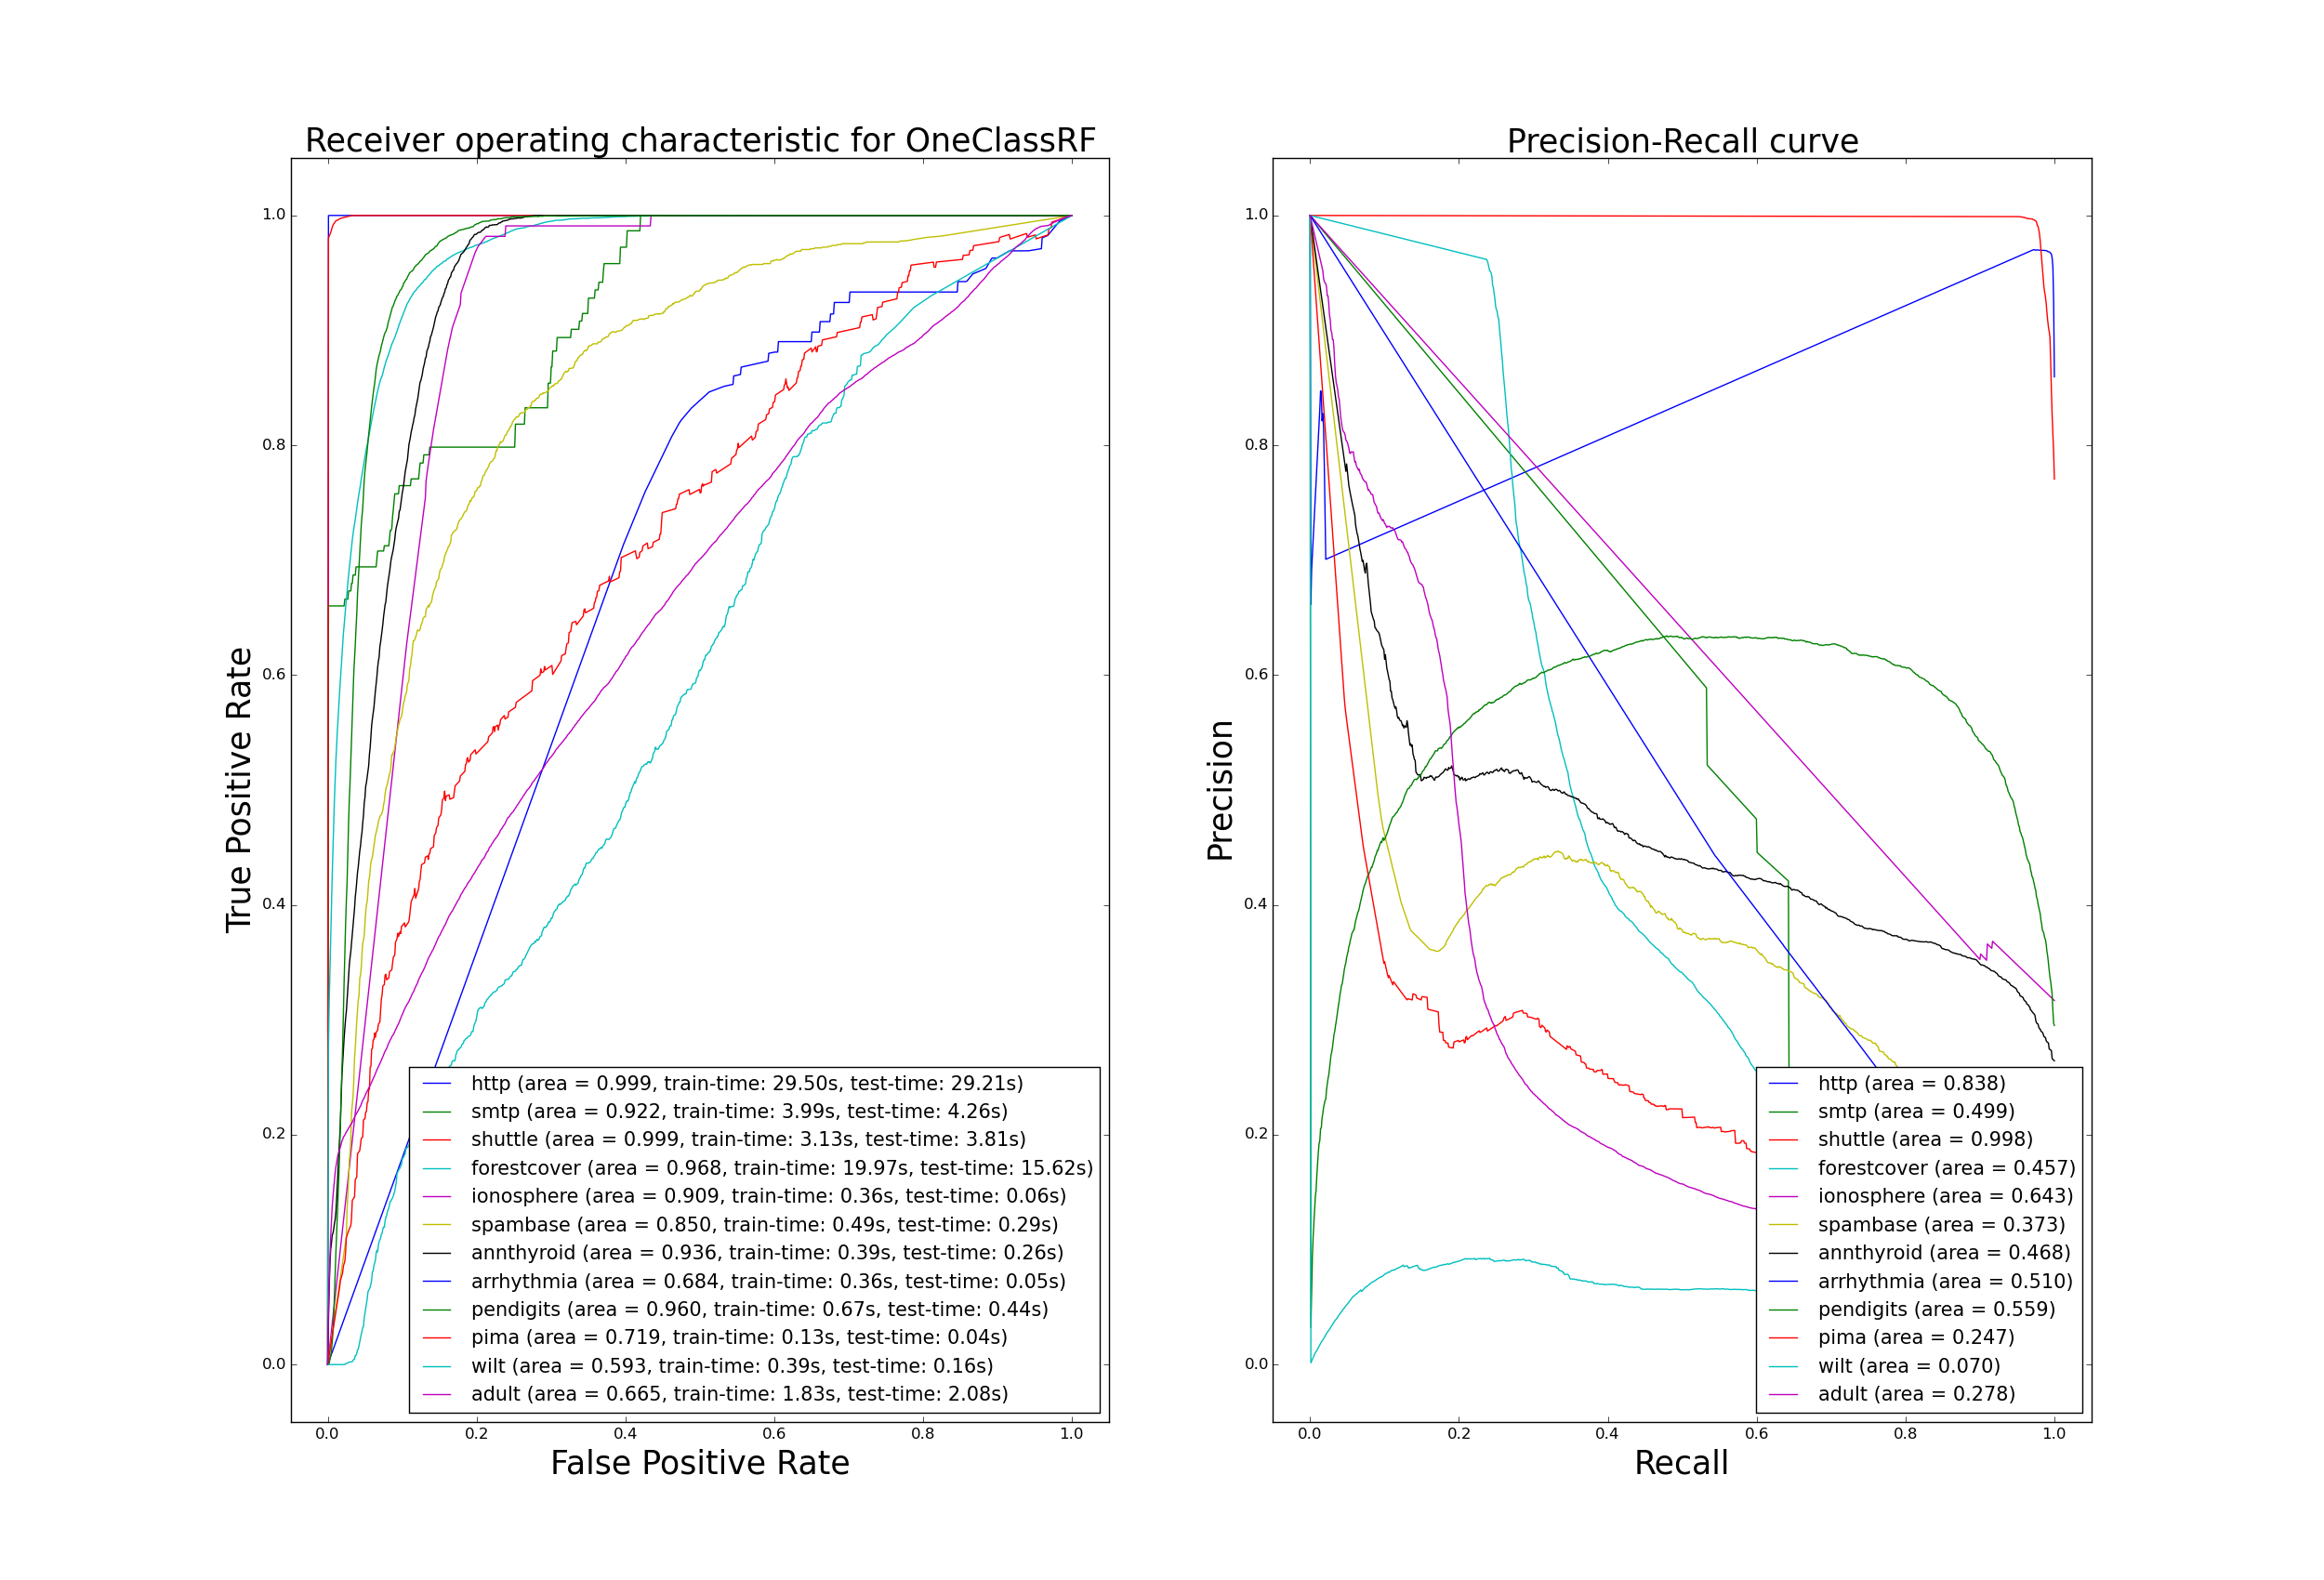
\includegraphics[trim=175 80 175 123, clip, width=0.992\linewidth]{fig_source/ocrf_fig/bench_oneclassrf_roc_pr_supervised_factorized.png}
\end{figure}
\begin{figure}[!ht]
  \caption{ROC and PR curves for OneClassRF (unsupervised framework)}
  \label{ocrf:fig:oneclassrf_roc_pr_unsupervised}
  \centering
  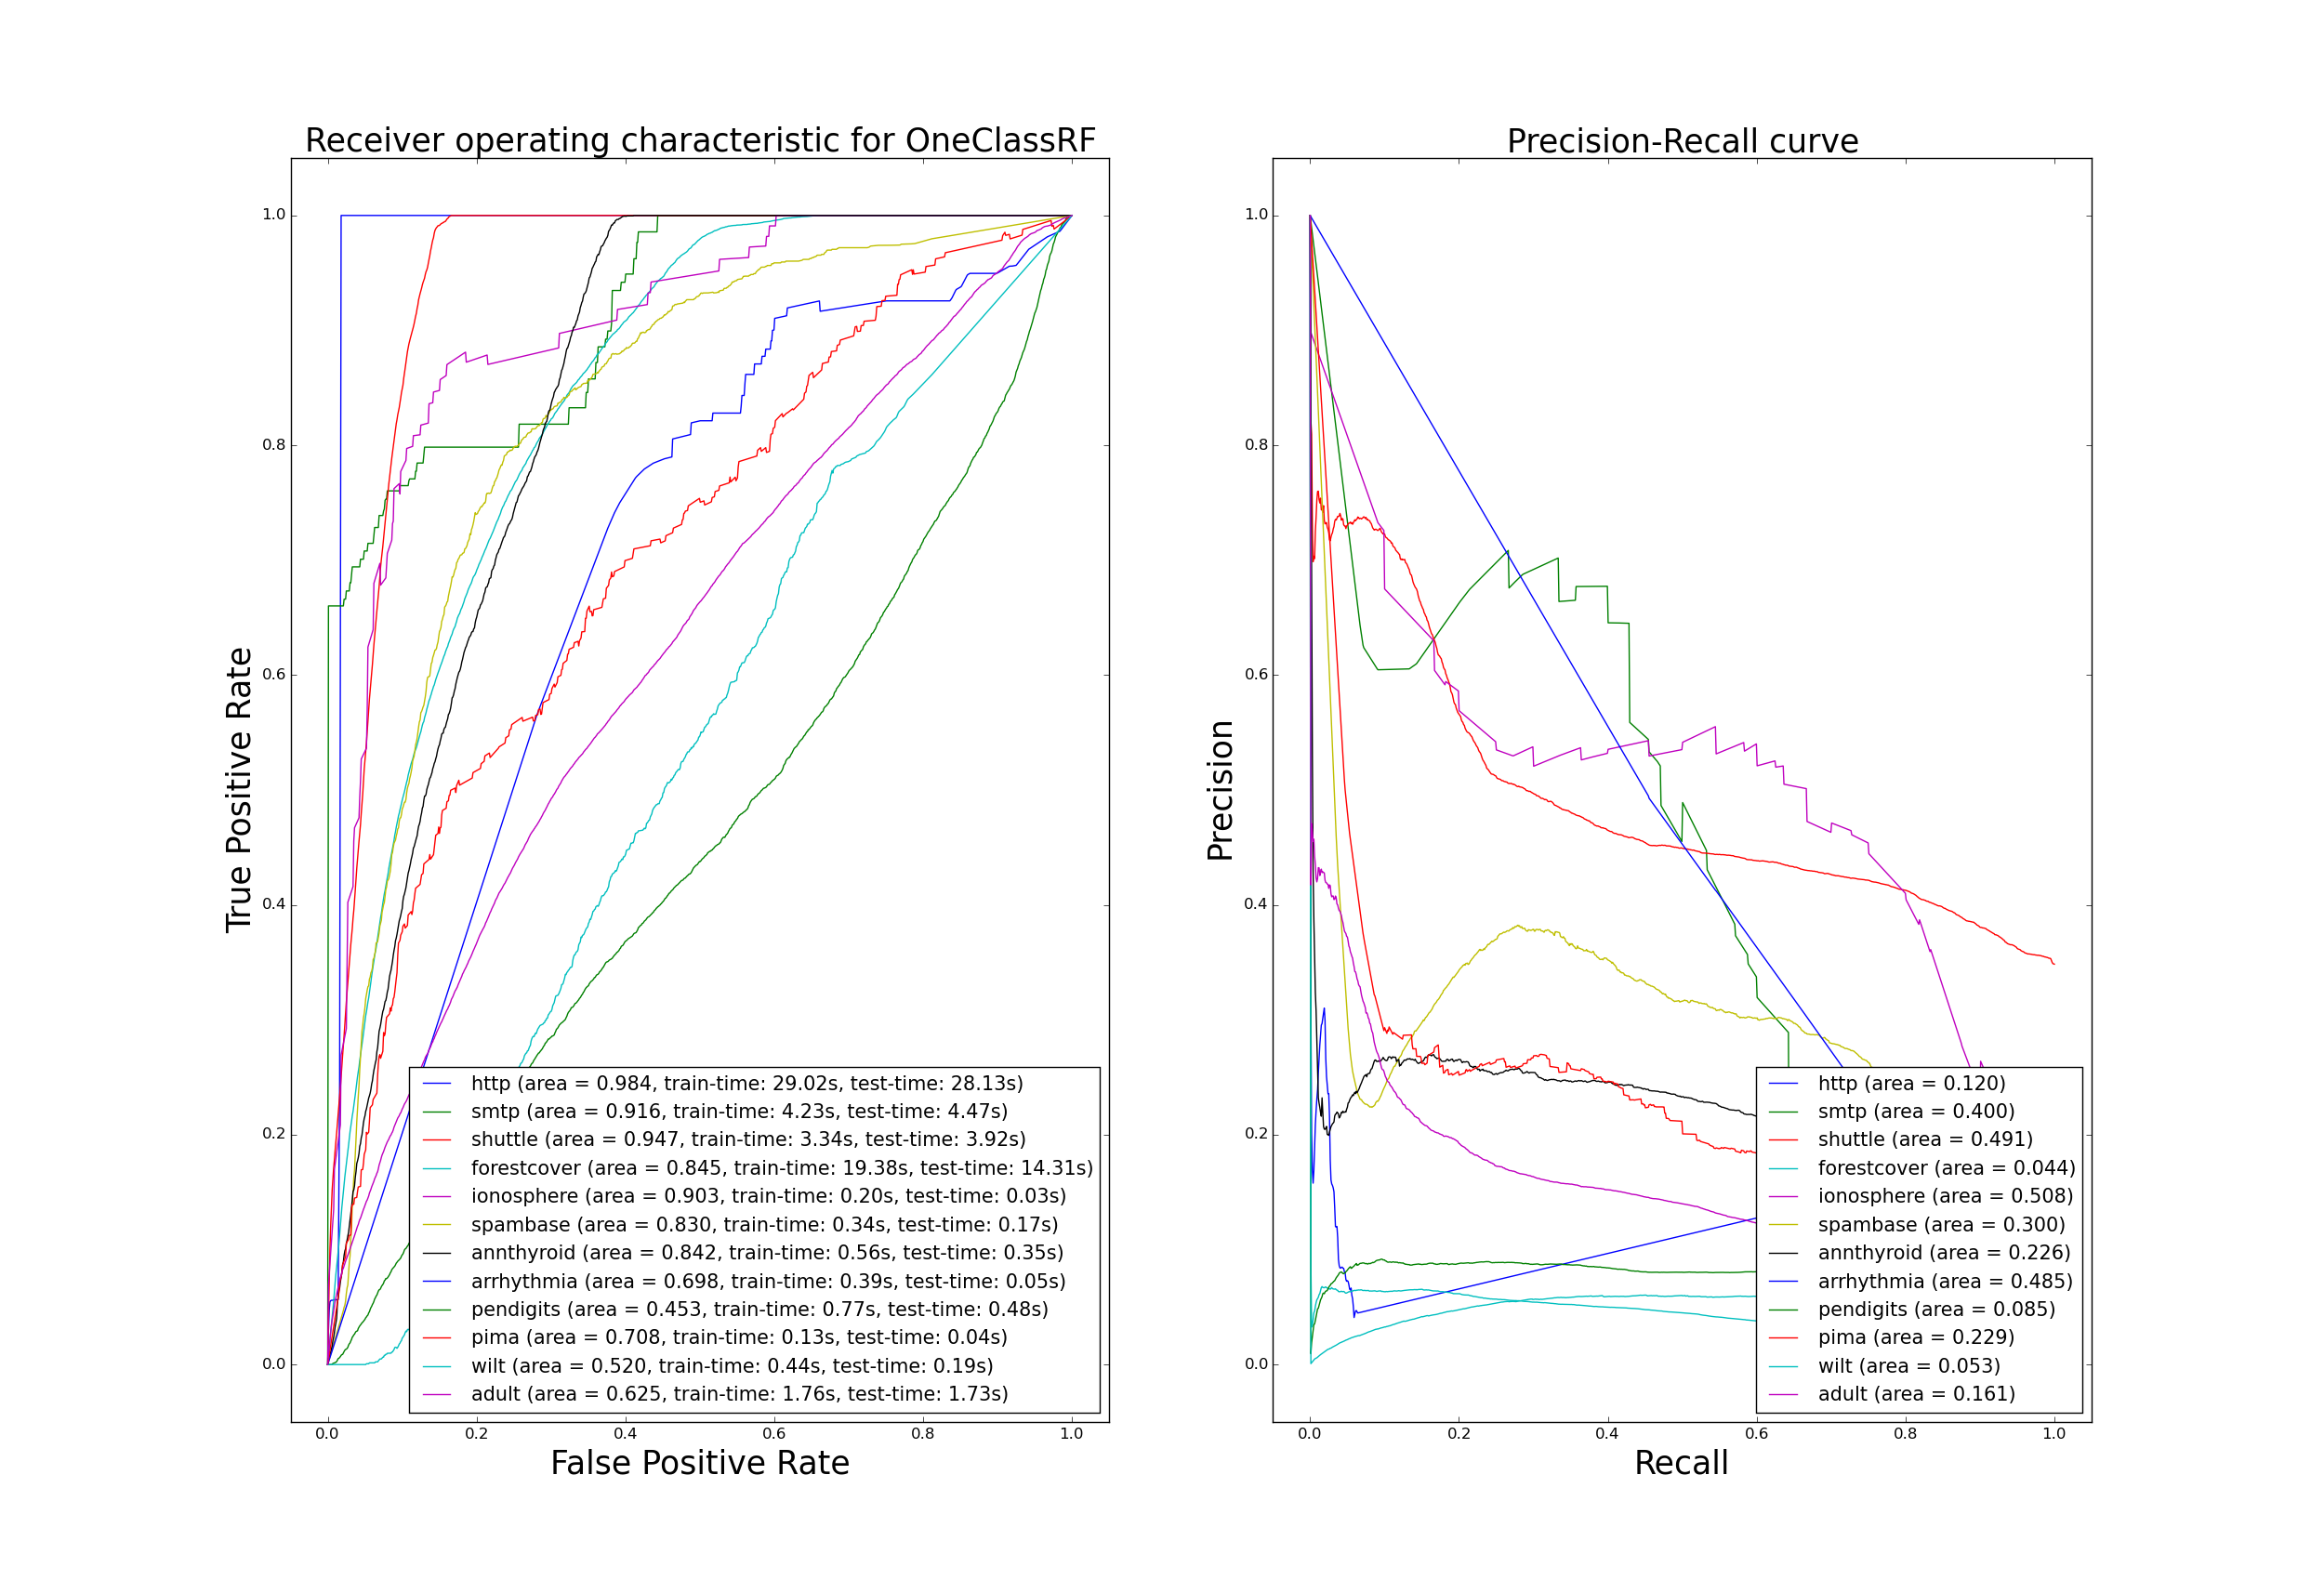
\includegraphics[trim=175 80 175 123, clip, width=0.992\linewidth]{fig_source/ocrf_fig/bench_oneclassrf_roc_pr_unsupervised_factorized.png}
\end{figure}

\begin{figure}[!ht]
  \caption{ROC and PR curves for IsolationForest (novelty detection framework)}
  \label{ocrf:fig:iforest_roc_pr}
  \centering
  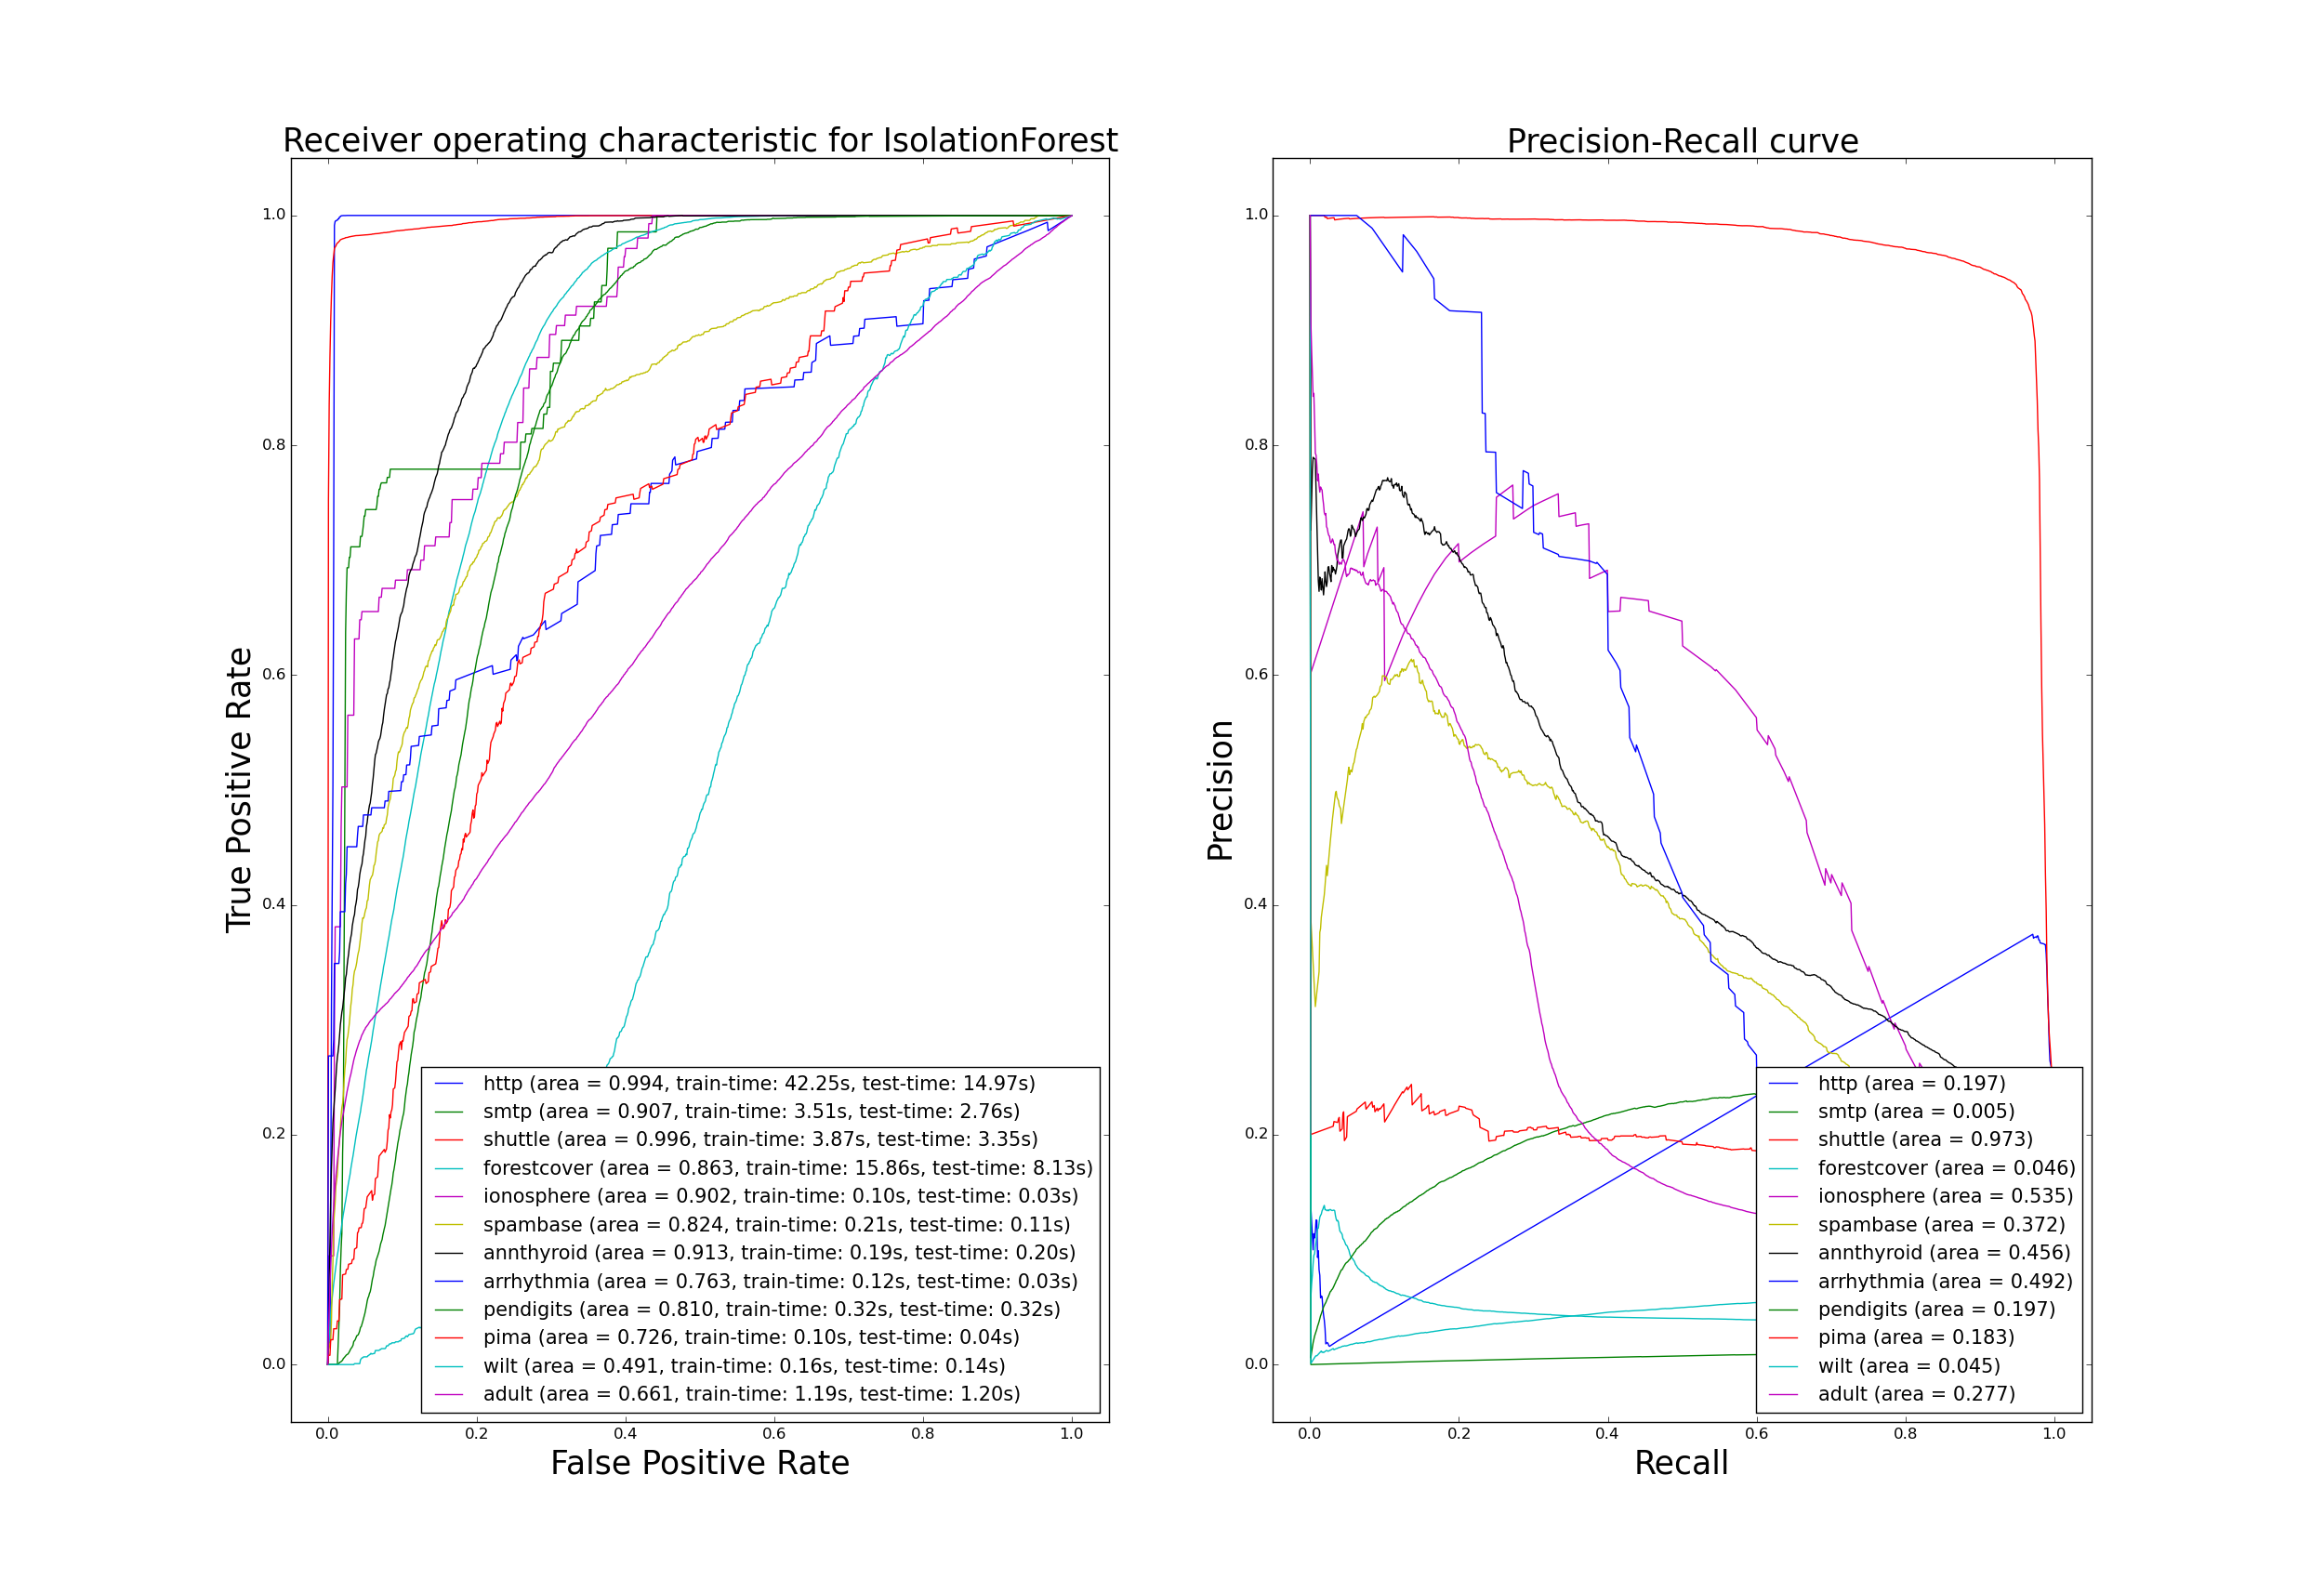
\includegraphics[trim=175 80 175 123, clip, width=\linewidth]{fig_source/ocrf_fig/bench_iforest_roc_pr_supervised_factorized.png}
\end{figure}
\begin{figure}[!ht]
  \caption{ROC and PR curves for IsolationForest (unsupervised framework)}
  \label{ocrf:fig:iforest_roc_pr_unsupervised}
  \centering
  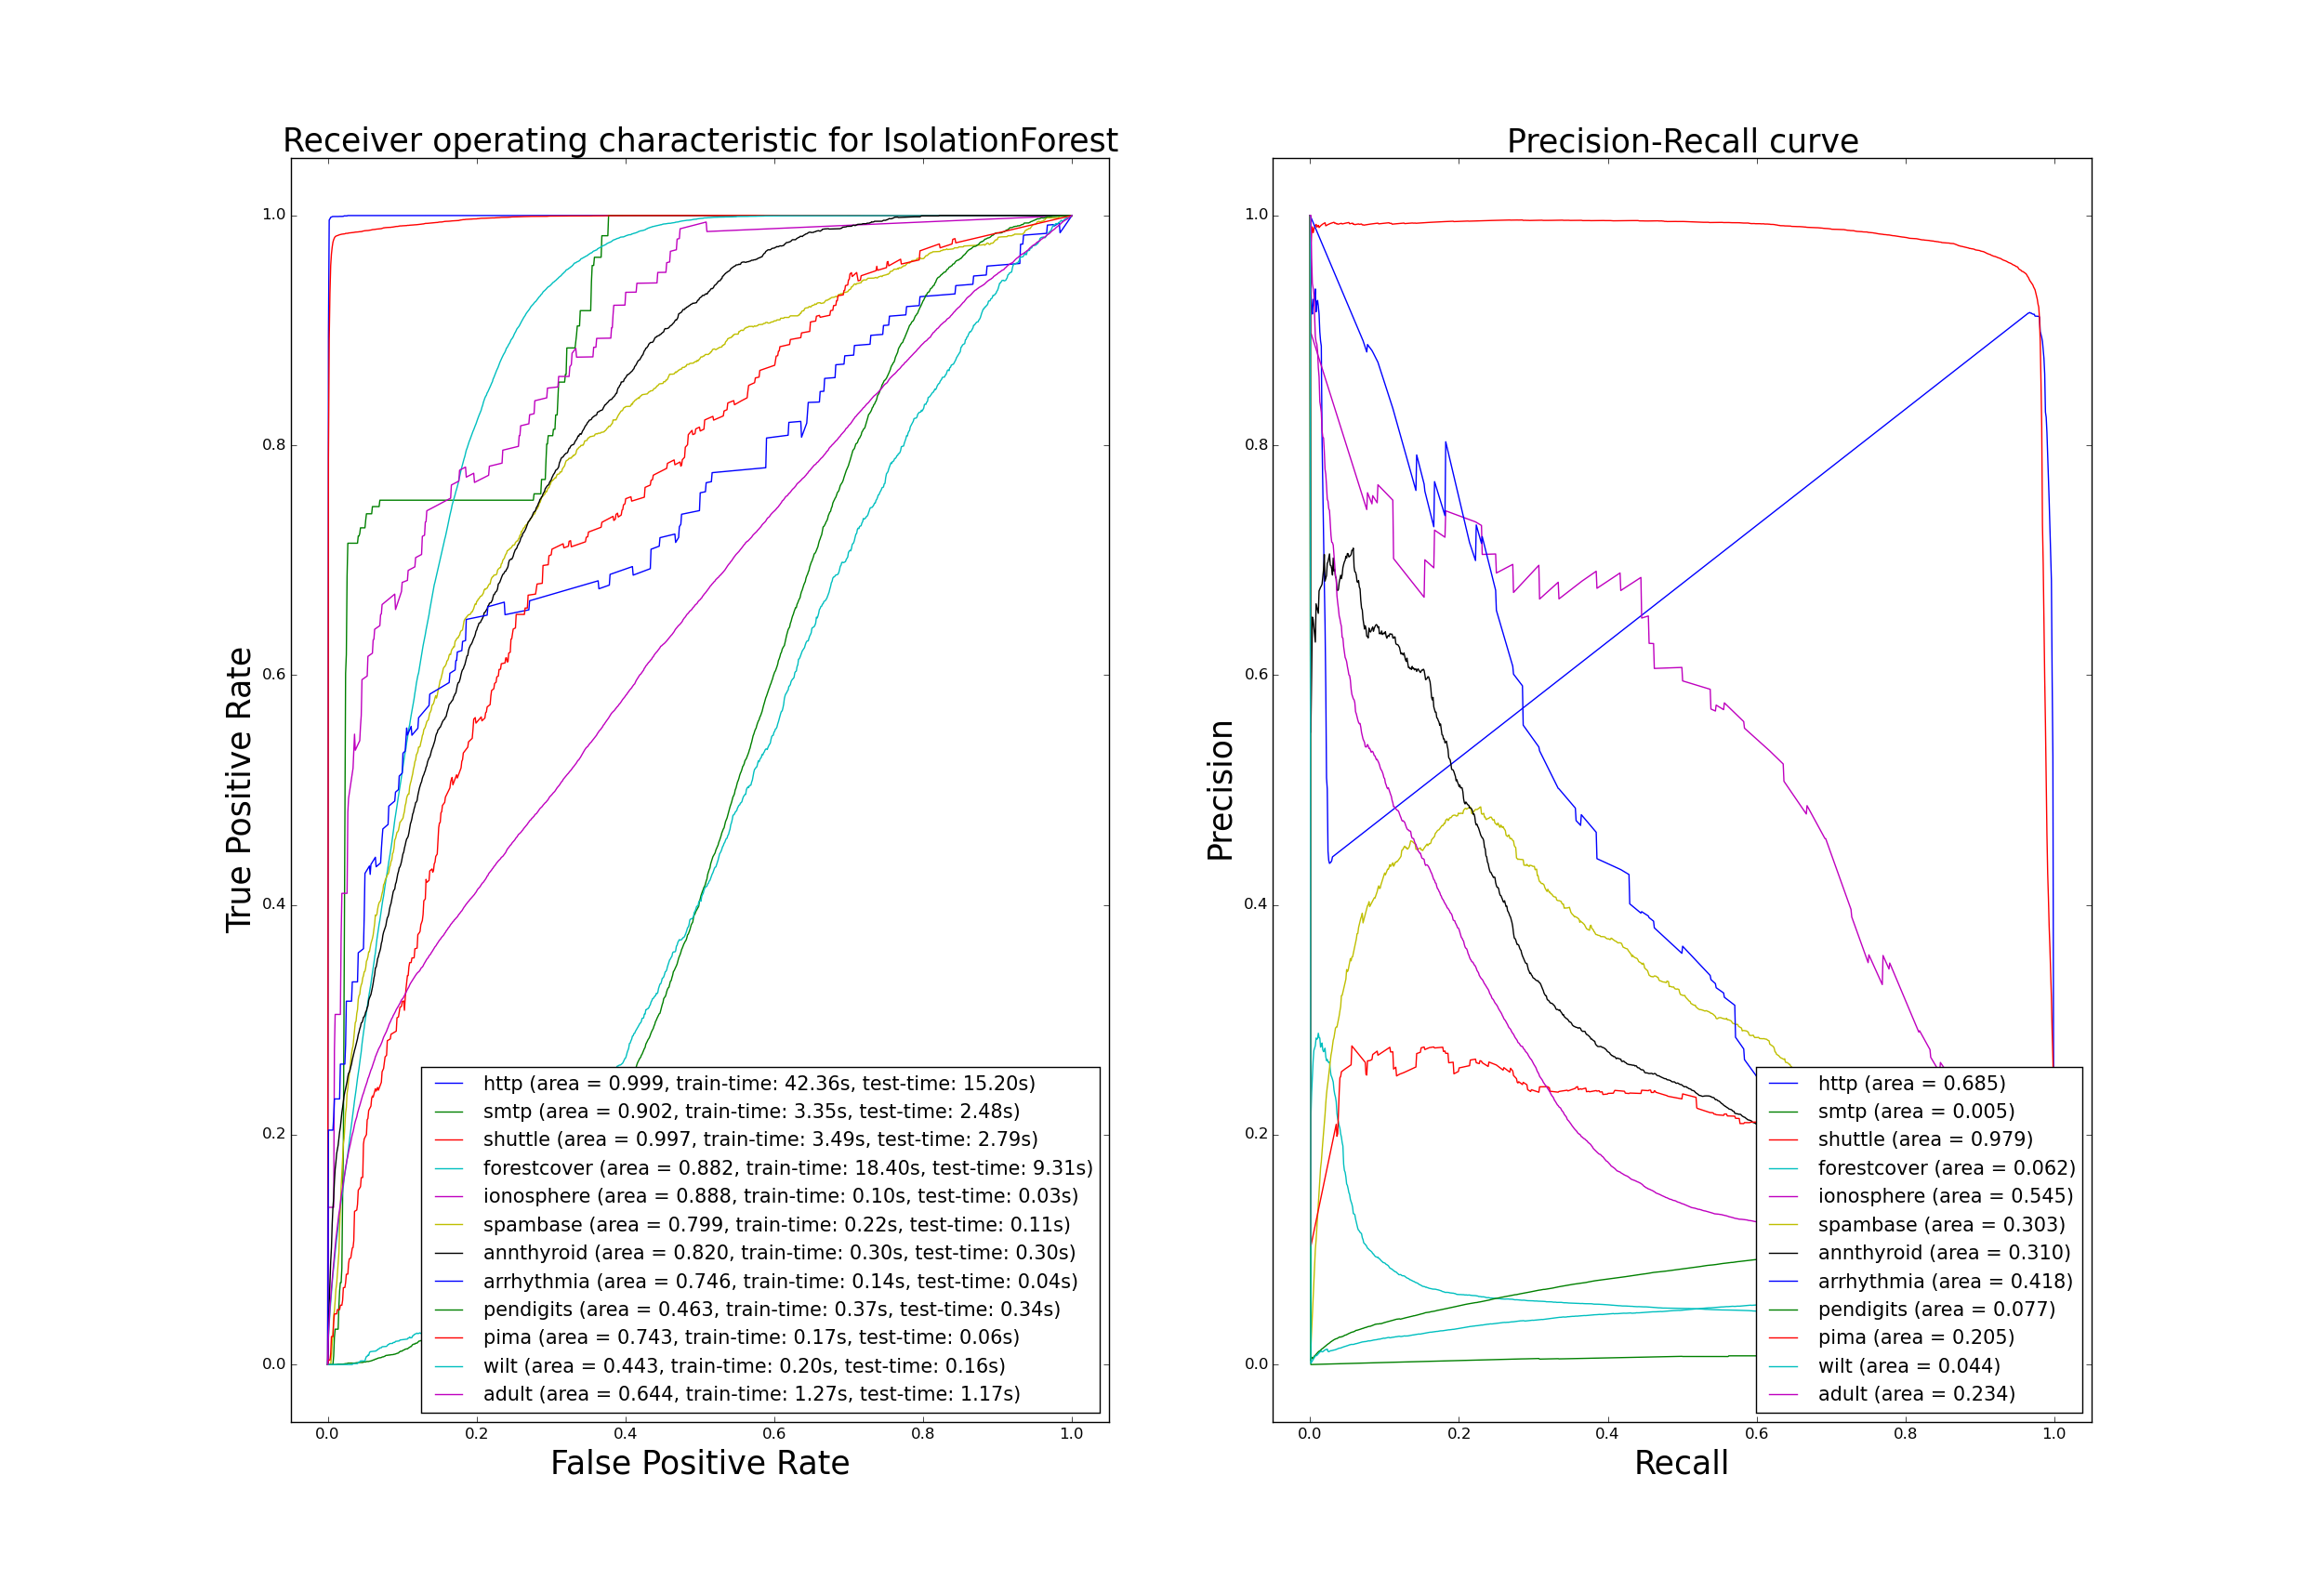
\includegraphics[trim=175 80 175 123, clip, width=\linewidth]{fig_source/ocrf_fig/bench_iforest_roc_pr_unsupervised_factorized.png}
\end{figure}

\begin{figure}[!ht]
  \caption{ROC and PR curves for OCRFsampling (novelty detection framework)}
  \label{ocrf:fig:ocrfm_roc_pr}
  \centering
  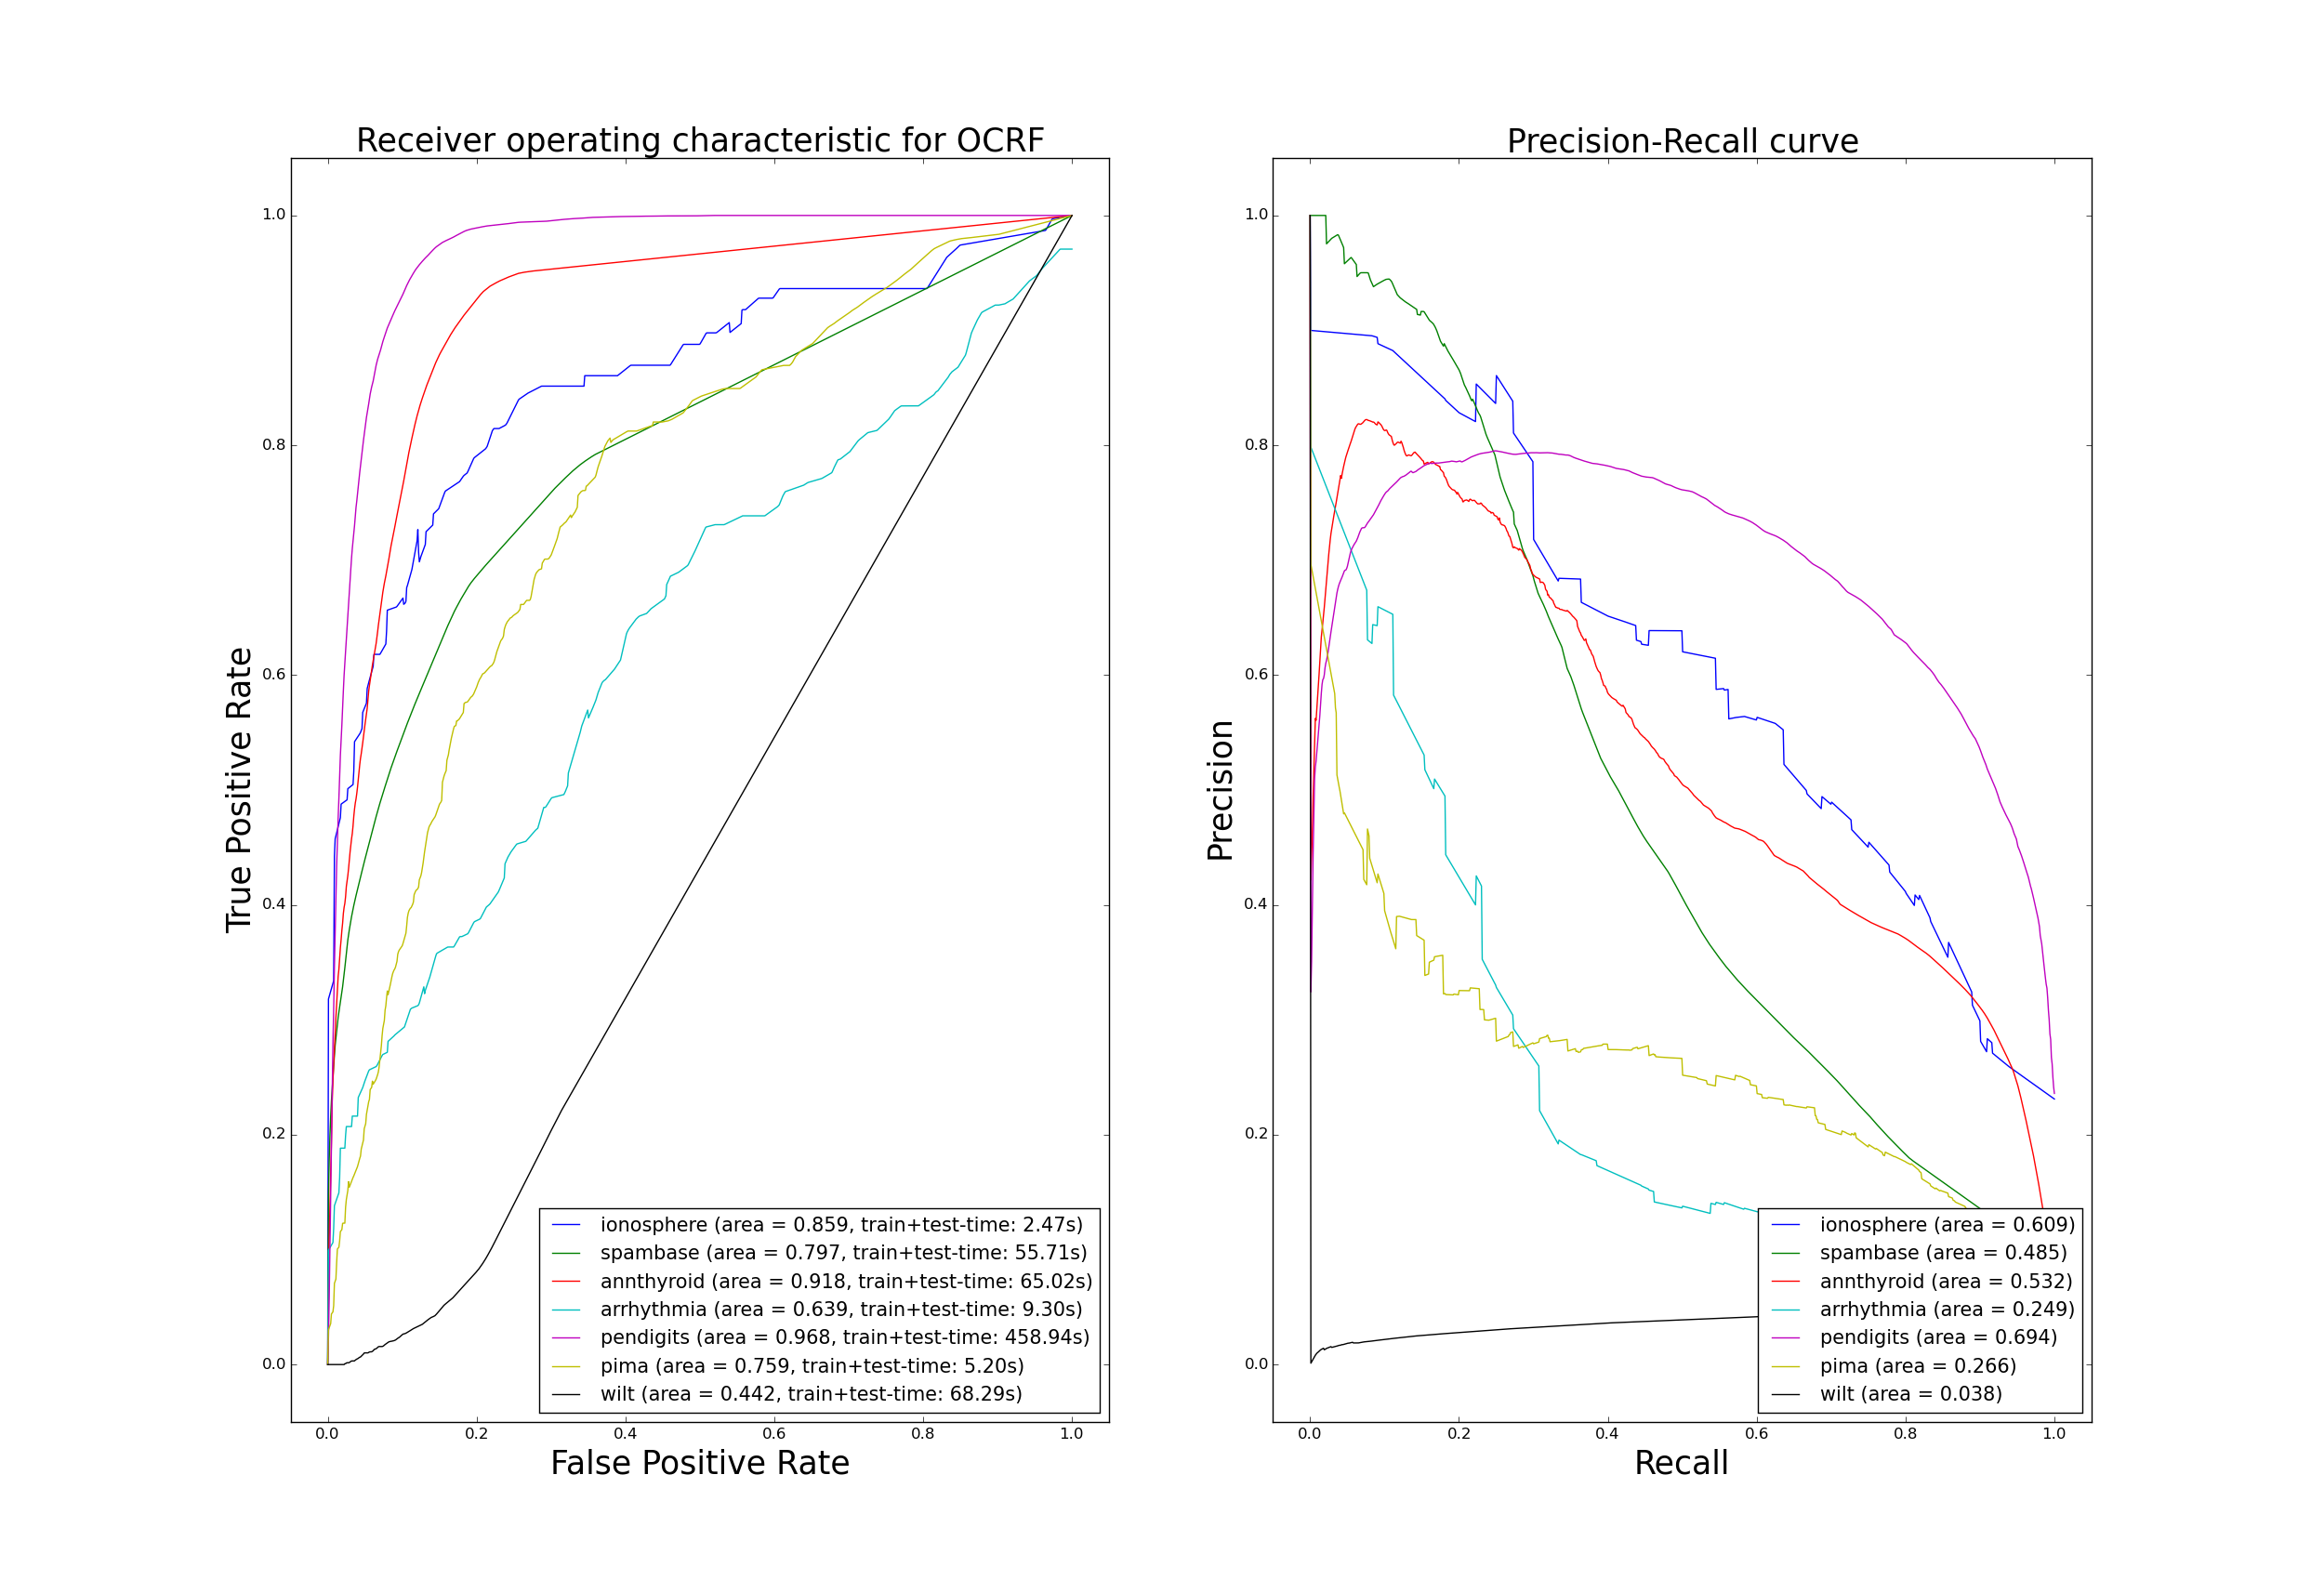
\includegraphics[trim=175 80 175 123, clip, width=\linewidth]{fig_source/ocrf_fig/bench_ocrf_roc_pr_supervised_factorized.png}
\end{figure}
\begin{figure}[!ht]
  \caption{ROC and PR curves for OCRFsampling (unsupervised framework)}
  \label{ocrf:fig:ocrfm_roc_pr_unsupervised}
  \centering
  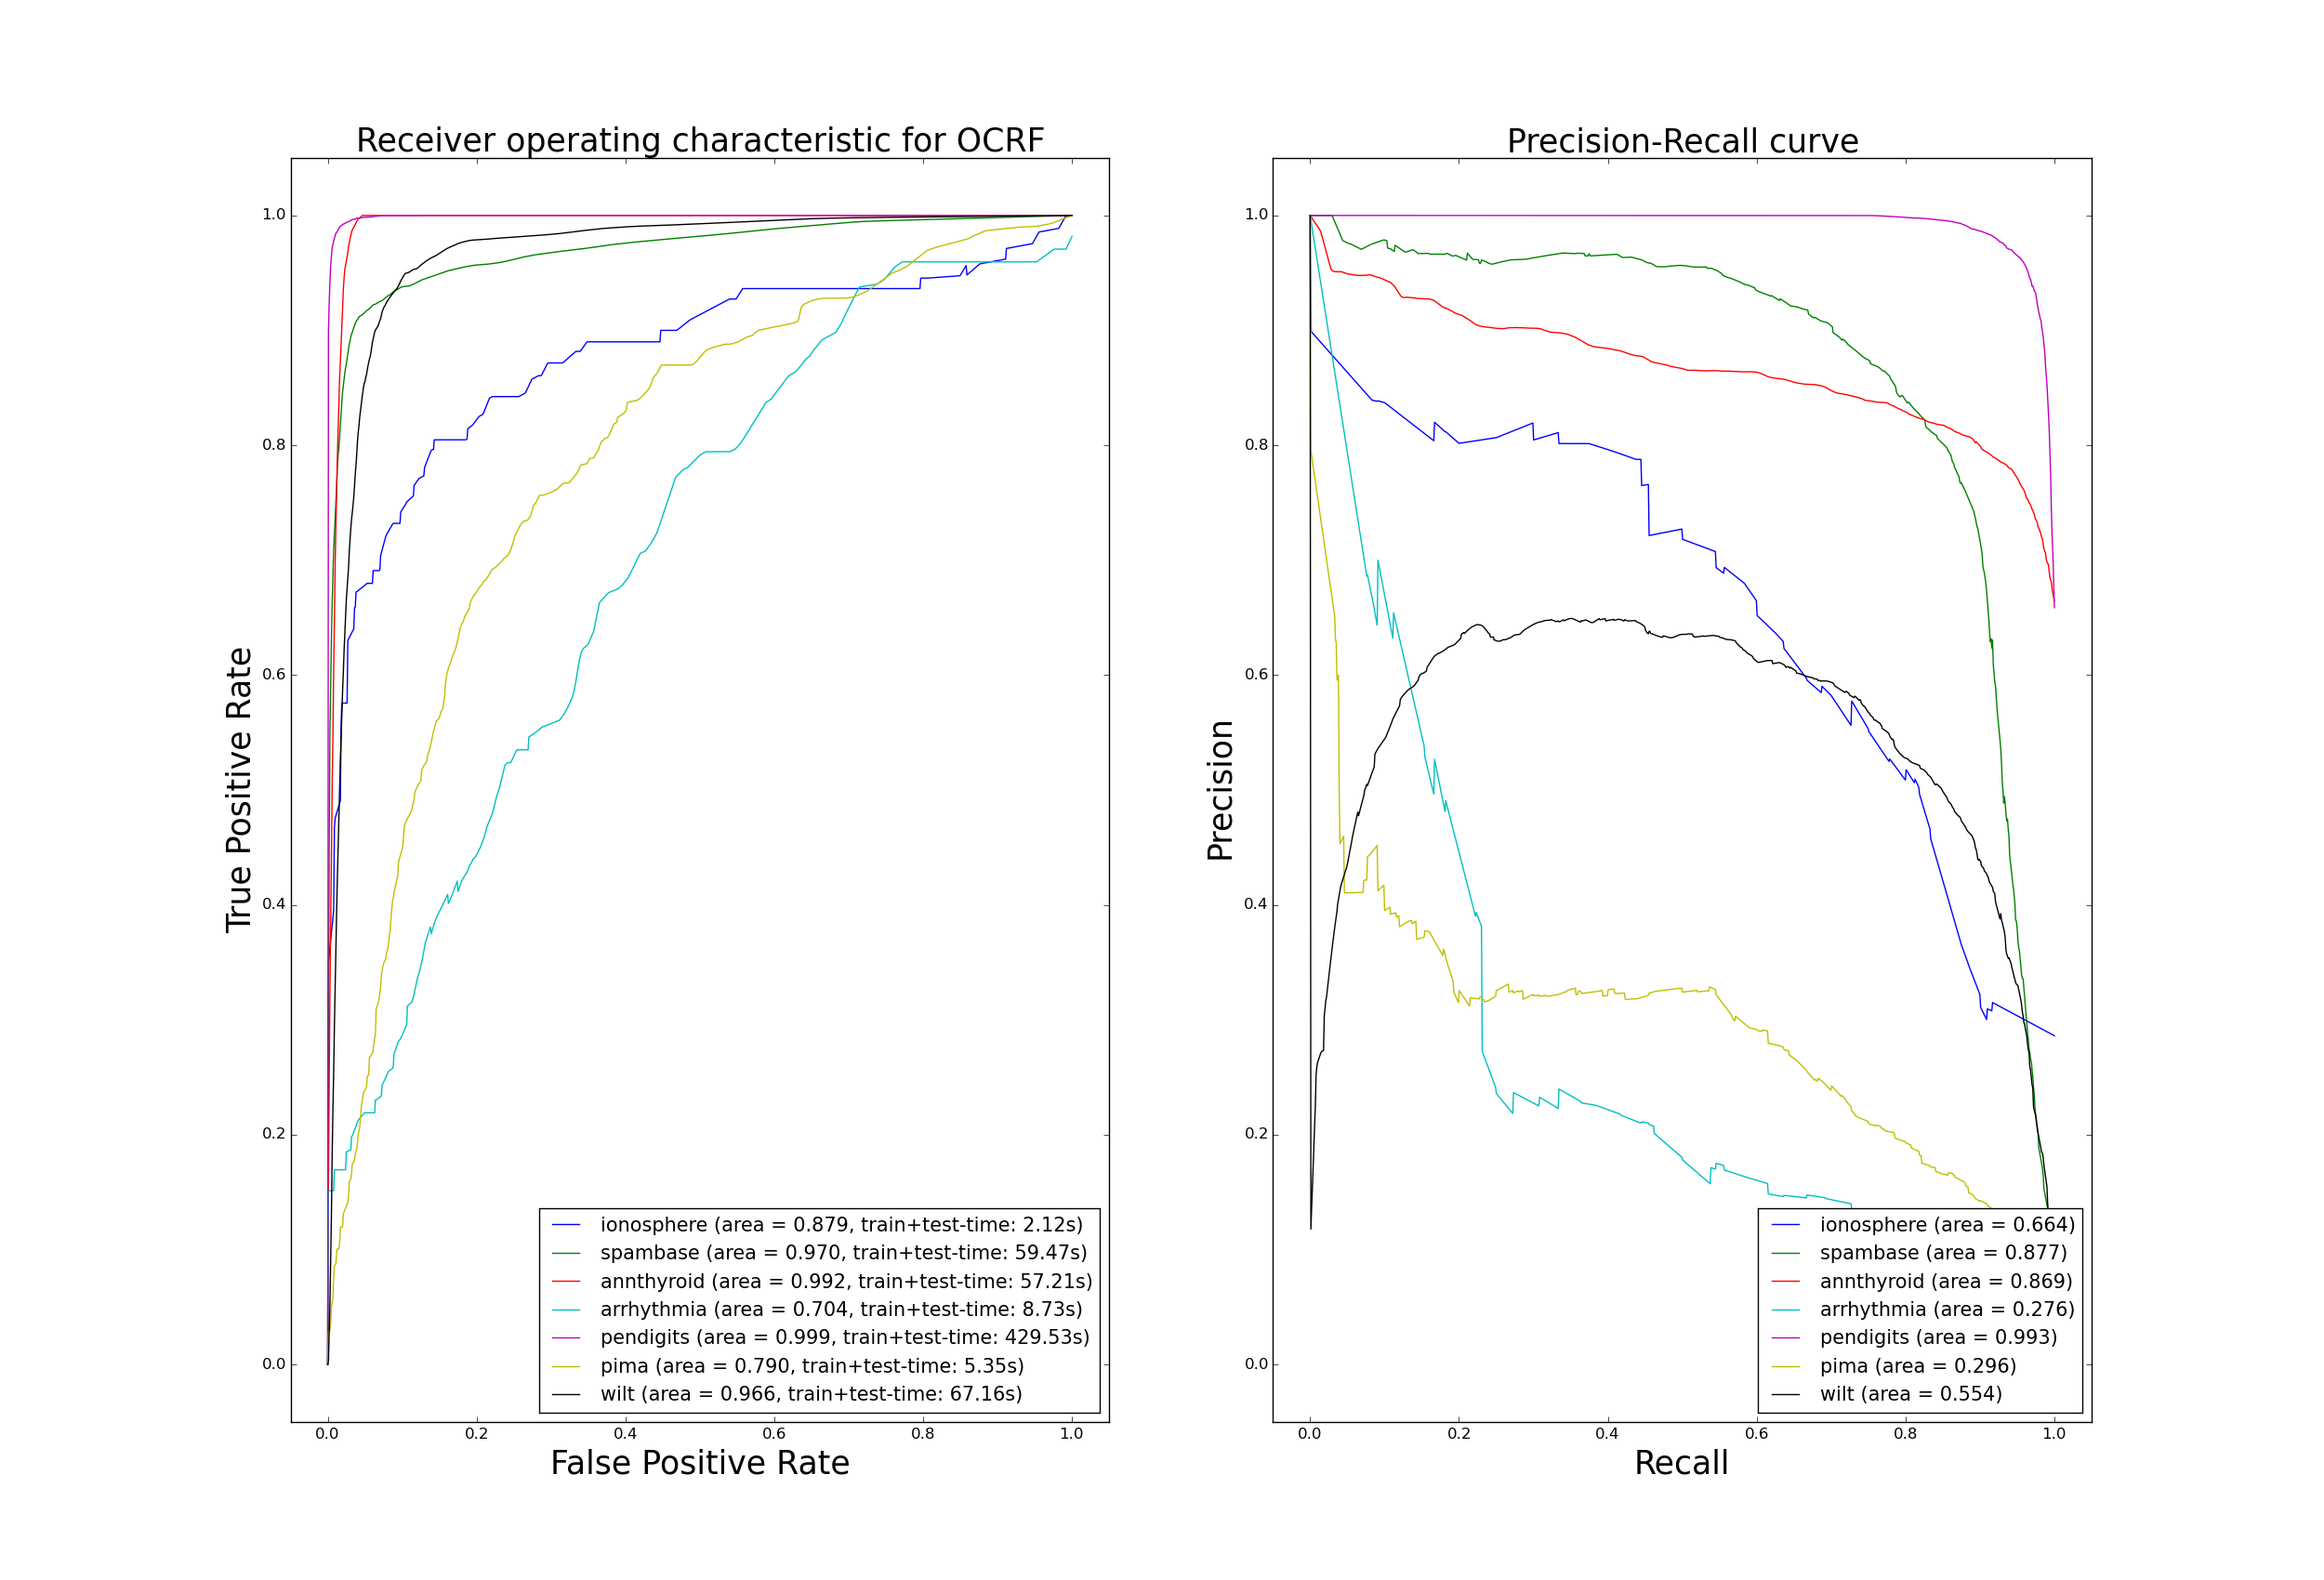
\includegraphics[trim=175 80 175 123, clip, width=\linewidth]{fig_source/ocrf_fig/bench_ocrf_roc_pr_unsupervised_factorized.png}
\end{figure}

\begin{figure}[!ht]
  \caption{ROC and PR curves for OCSVM (novelty detection framework)}
  \label{ocrf:fig:ocsvm_roc_pr}
  \centering
  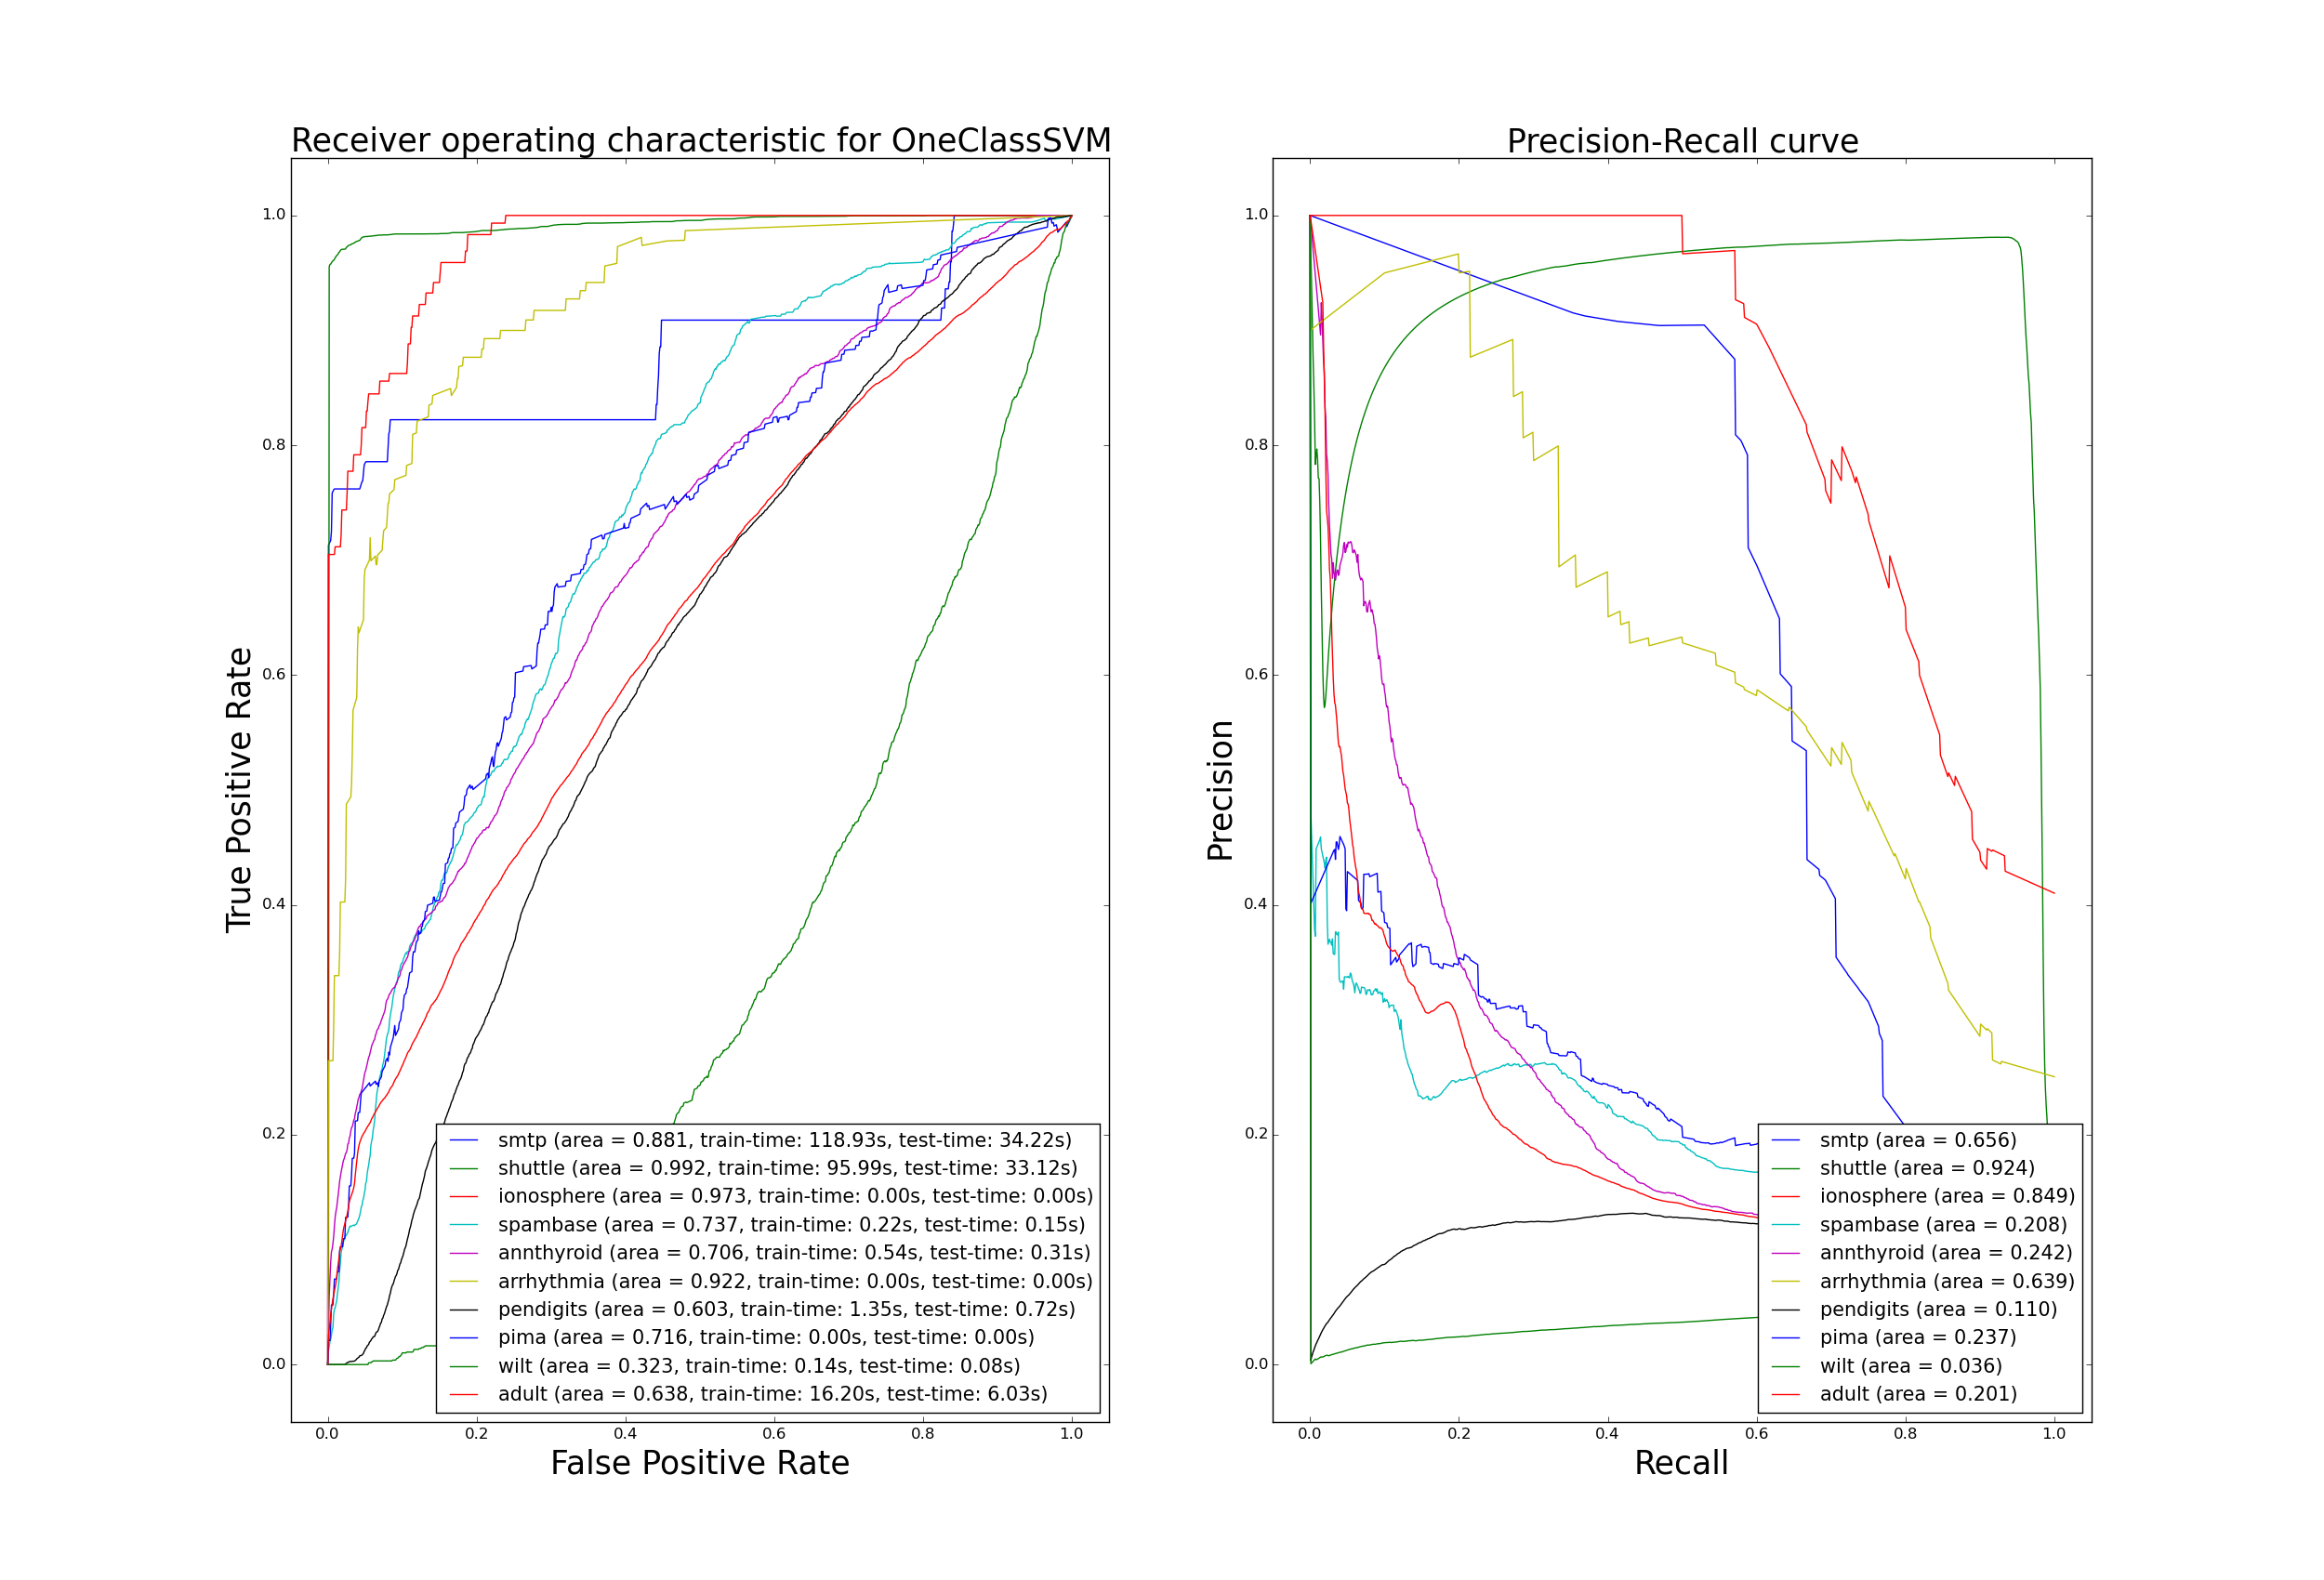
\includegraphics[trim=175 80 175 123, clip, width=\linewidth]{fig_source/ocrf_fig/bench_ocsvm_roc_pr_supervised_factorized.png}
\end{figure}
\begin{figure}[!ht]
  \caption{ROC and PR curves for OCSVM (unsupervised framework)}
  \label{ocrf:fig:ocsvm_roc_pr_unsupervised}
  \centering
  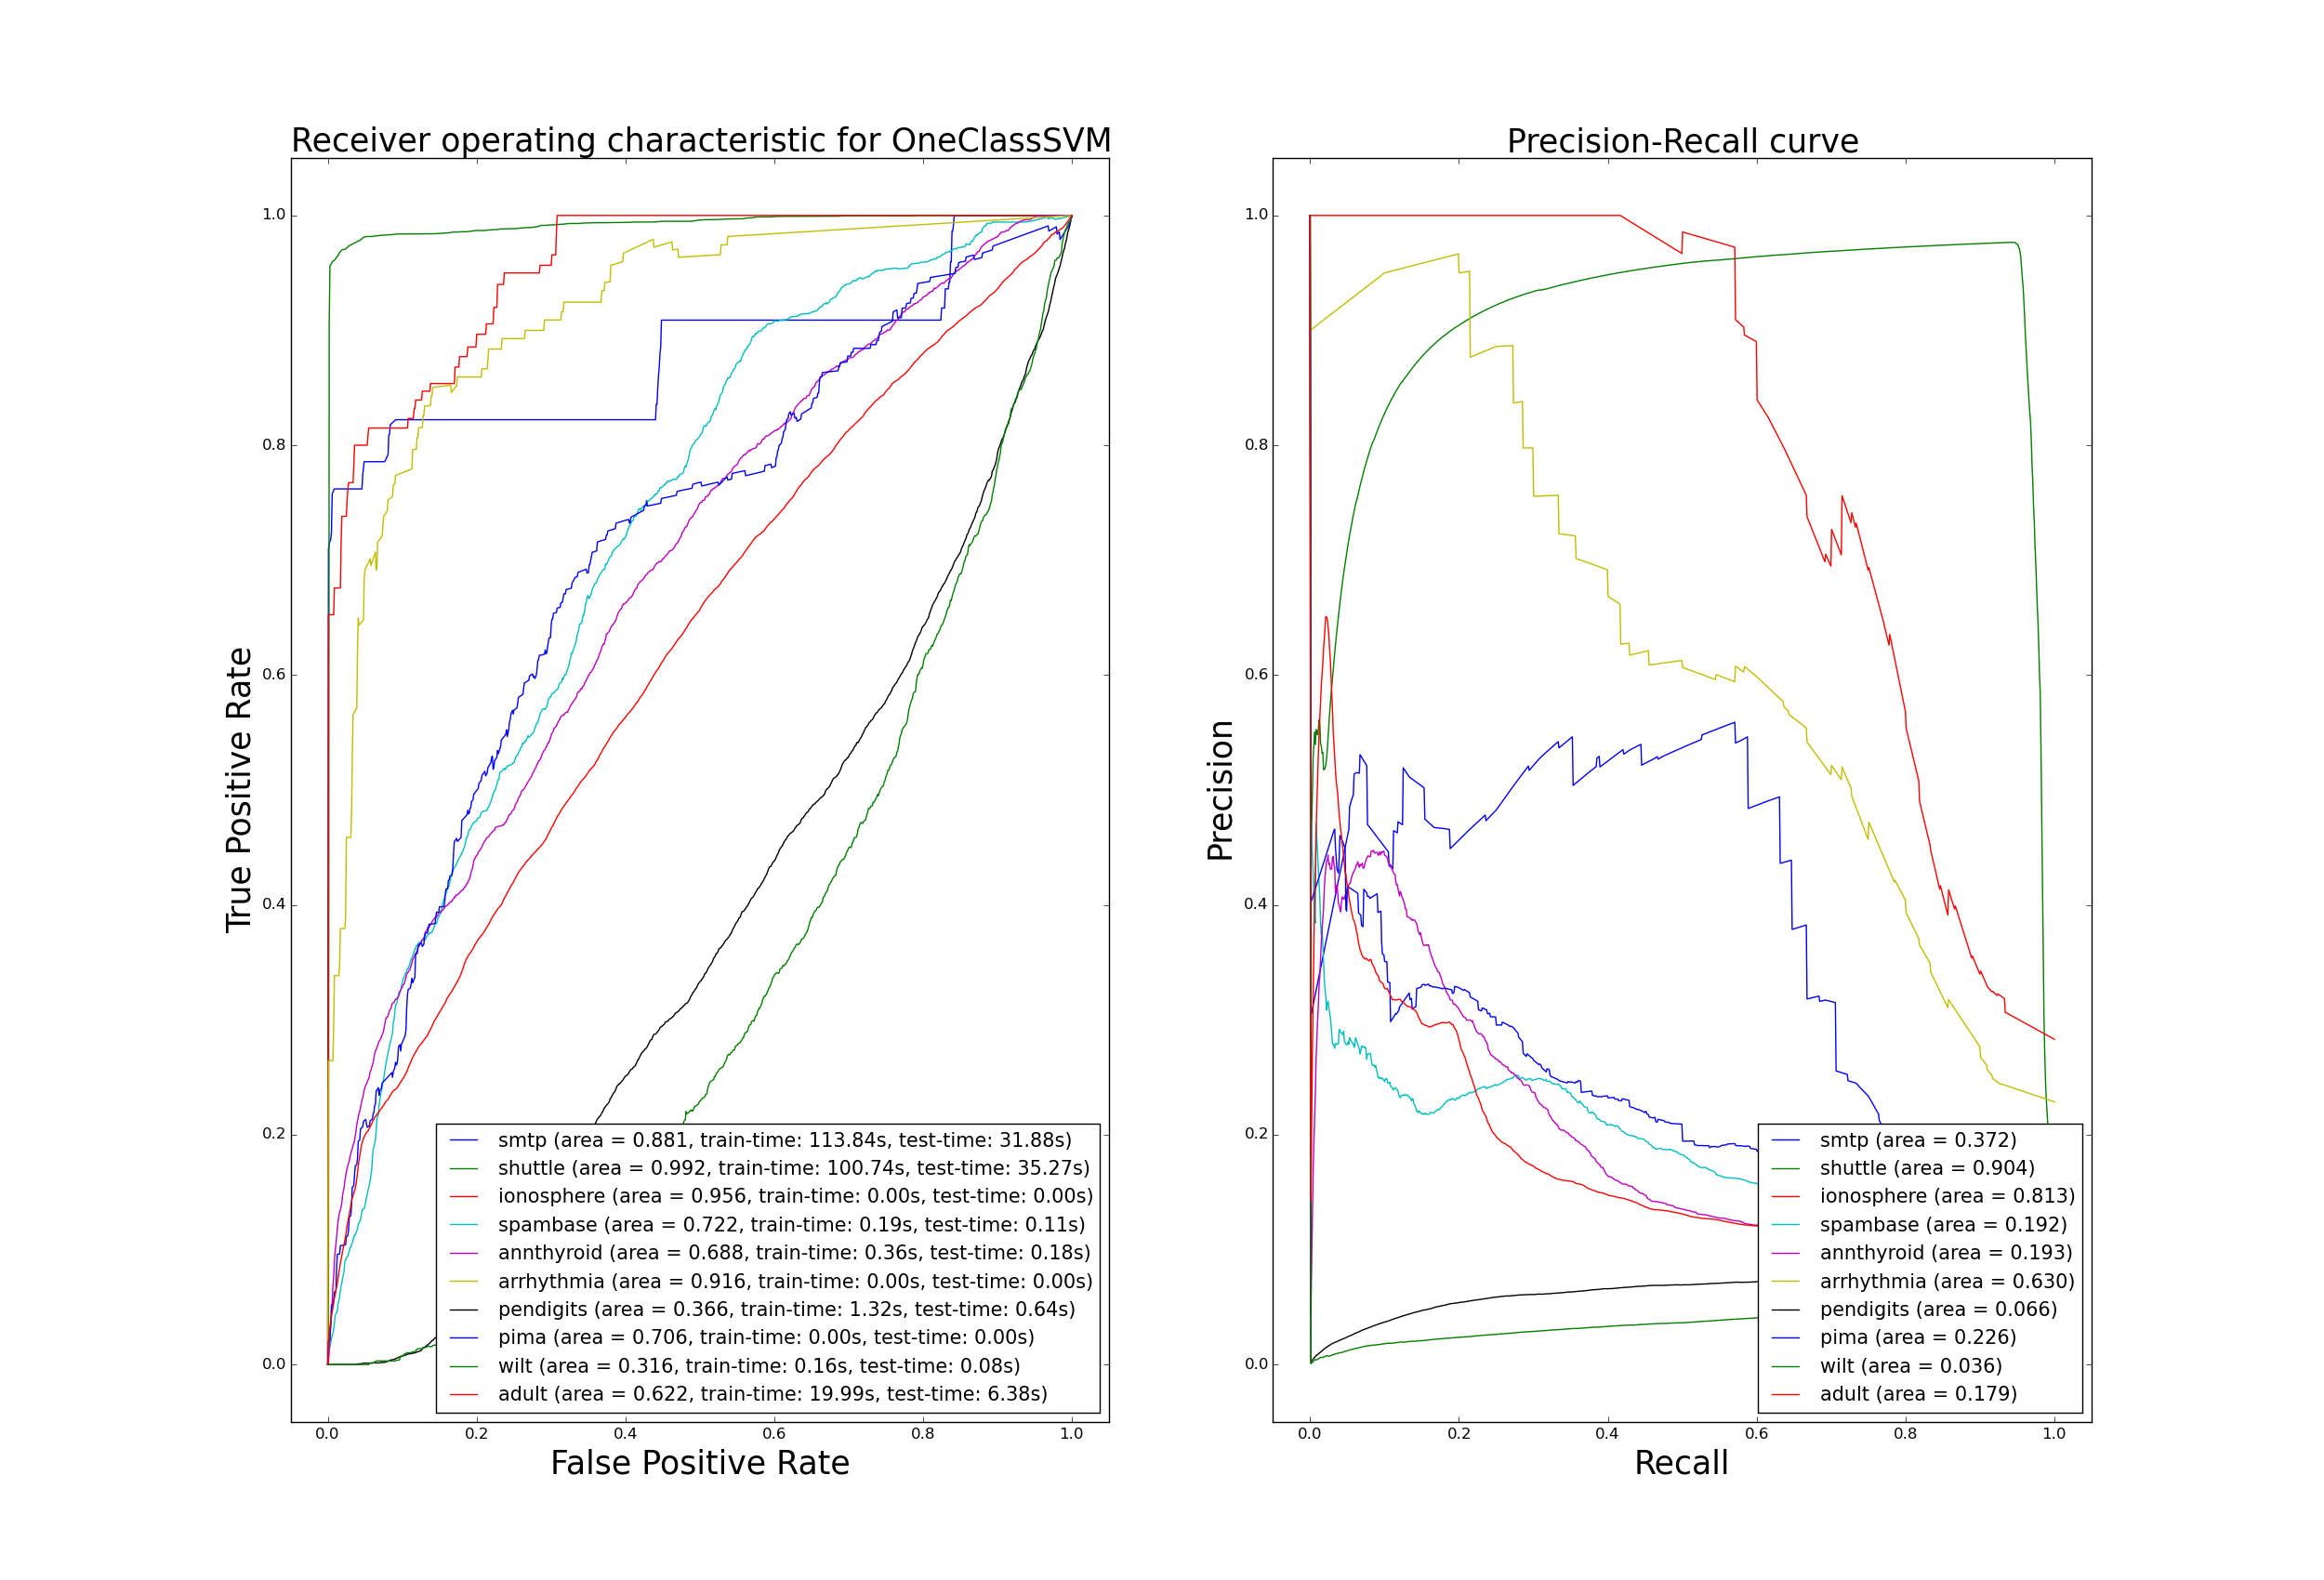
\includegraphics[trim=175 80 175 123, clip, width=\linewidth]{fig_source/ocrf_fig/bench_ocsvm_roc_pr_unsupervised_factorized.png}
\end{figure}

\begin{figure}[!ht]
  \caption{ROC and PR curves for LOF (novelty detection framework)}
  \label{ocrf:fig:lof_roc_pr}
  \centering
  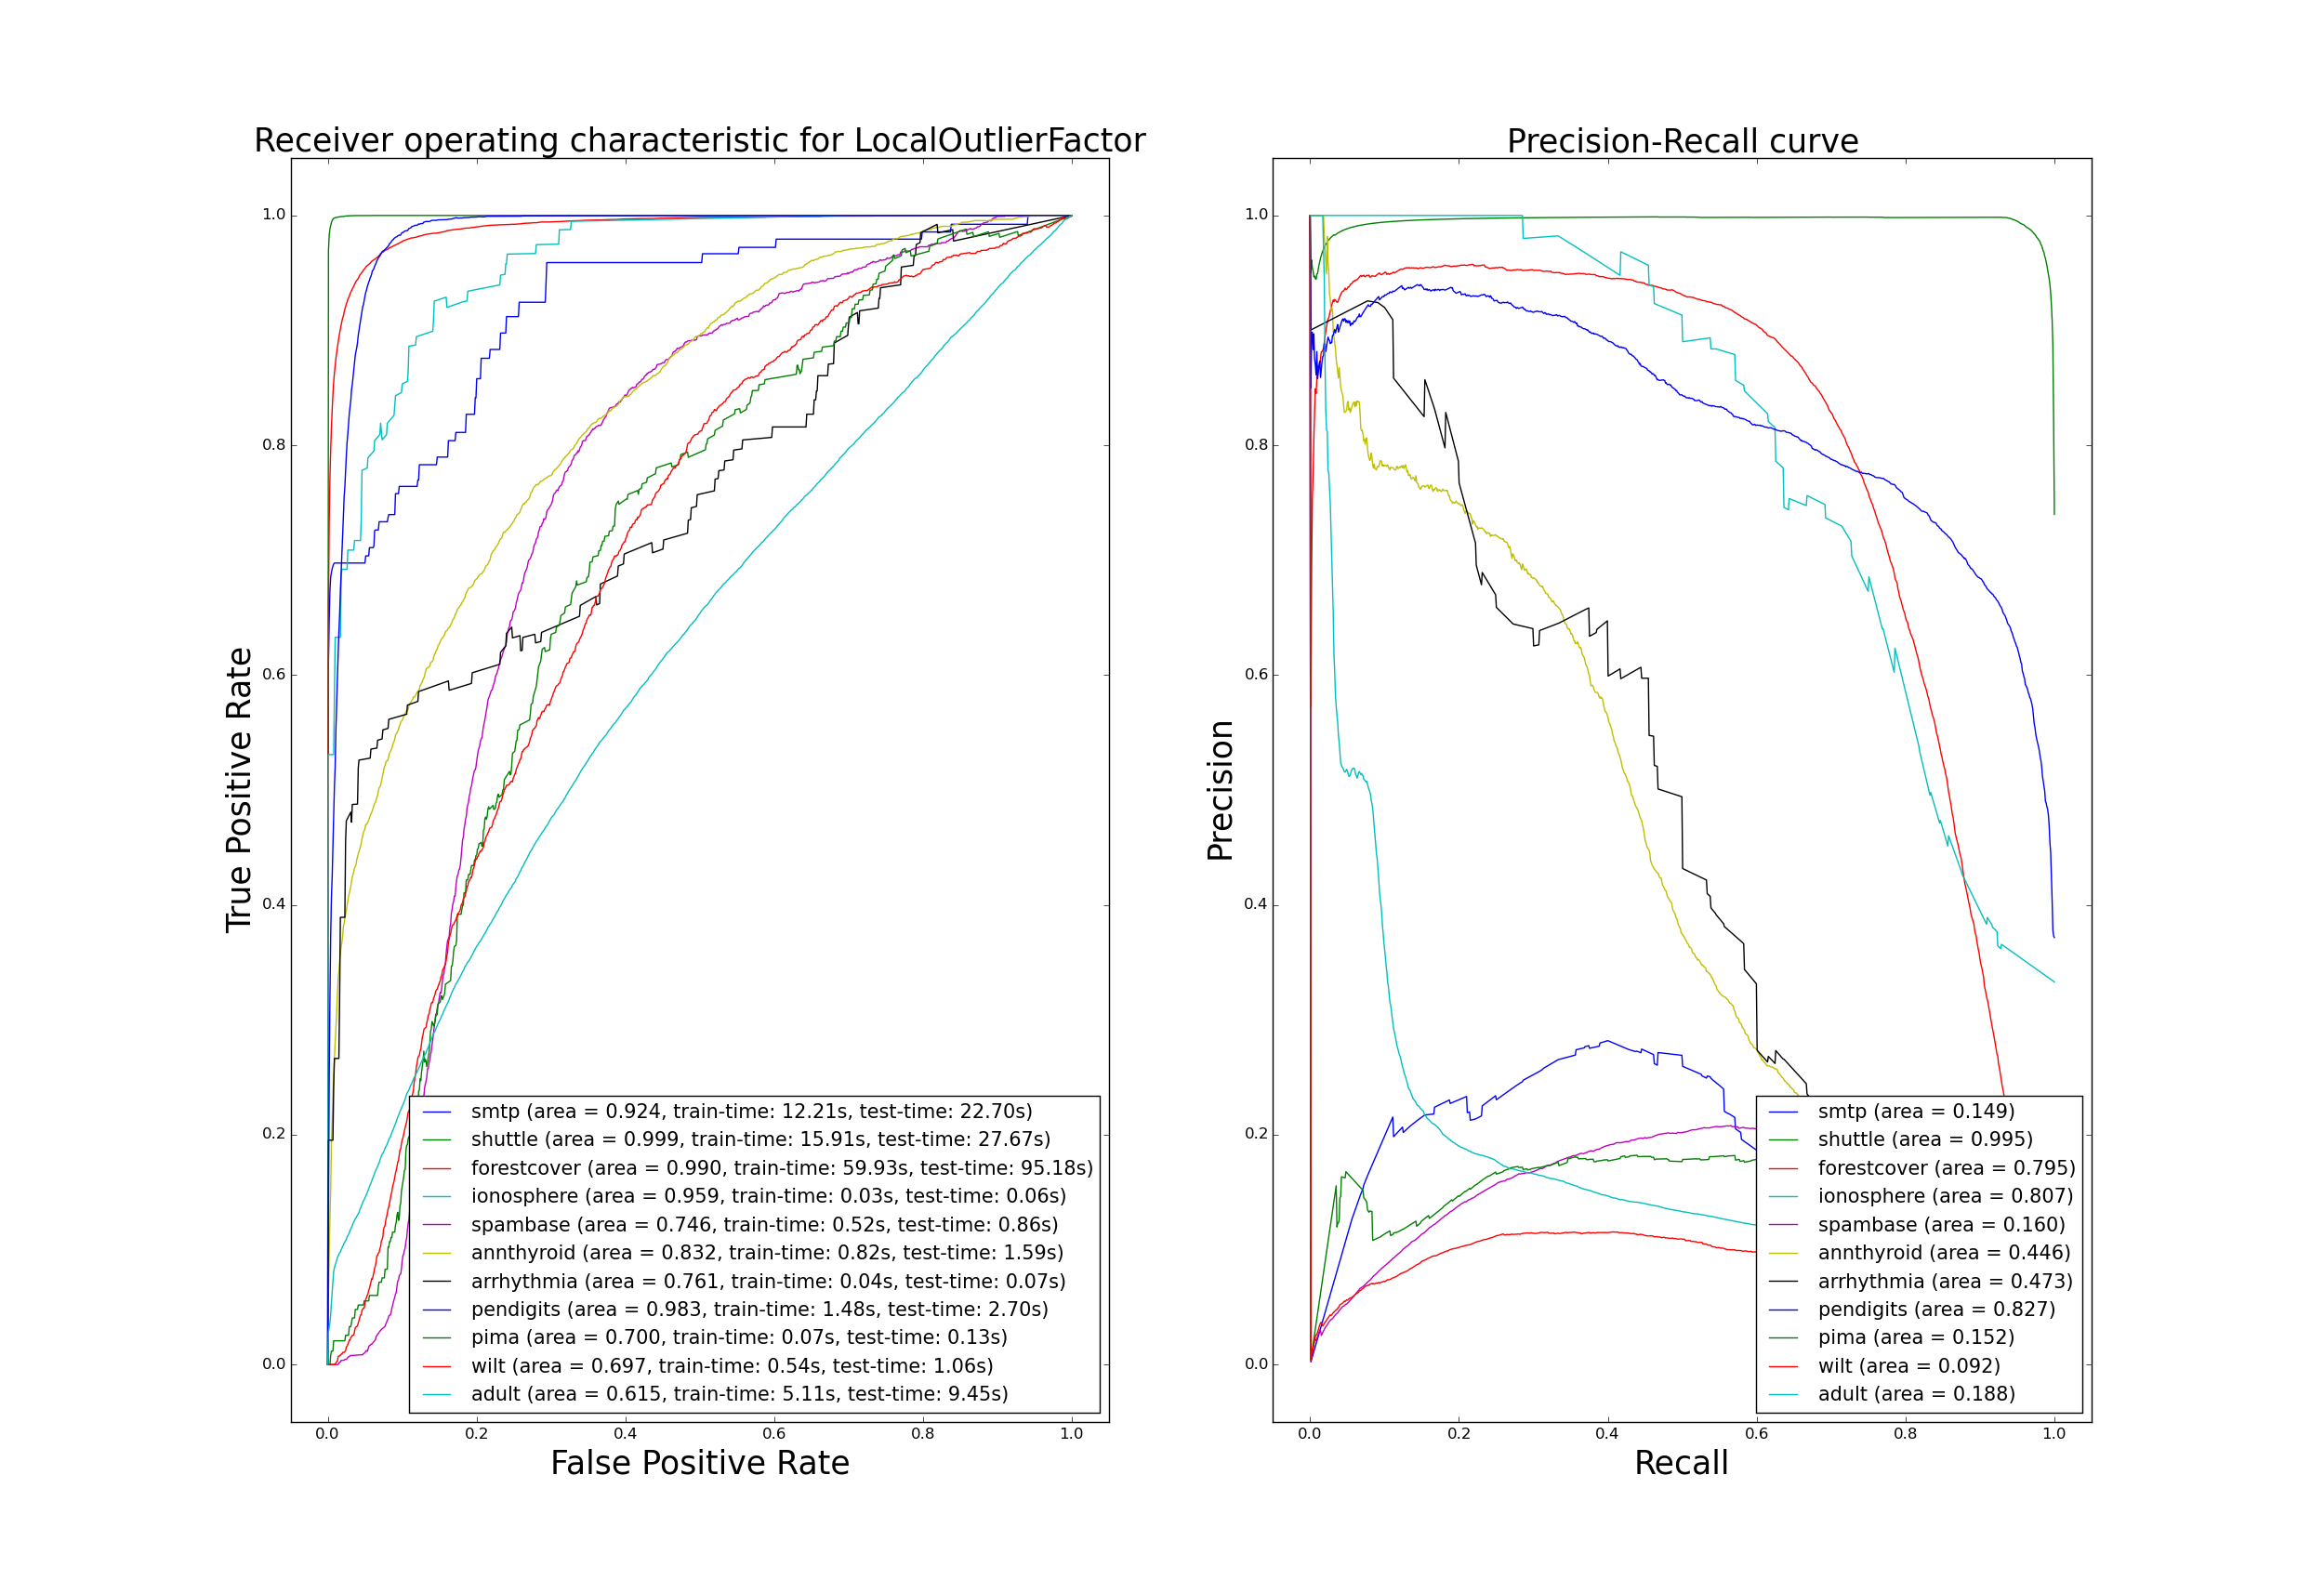
\includegraphics[trim=175 80 175 123, clip, width=\linewidth]{fig_source/ocrf_fig/bench_lof_roc_pr_supervised_factorized.png}
\end{figure}
\begin{figure}[!ht]
  \caption{ROC and PR curves for LOF (unsupervised framework)}
  \label{ocrf:fig:lof_roc_pr_unsupervised}
  \centering
  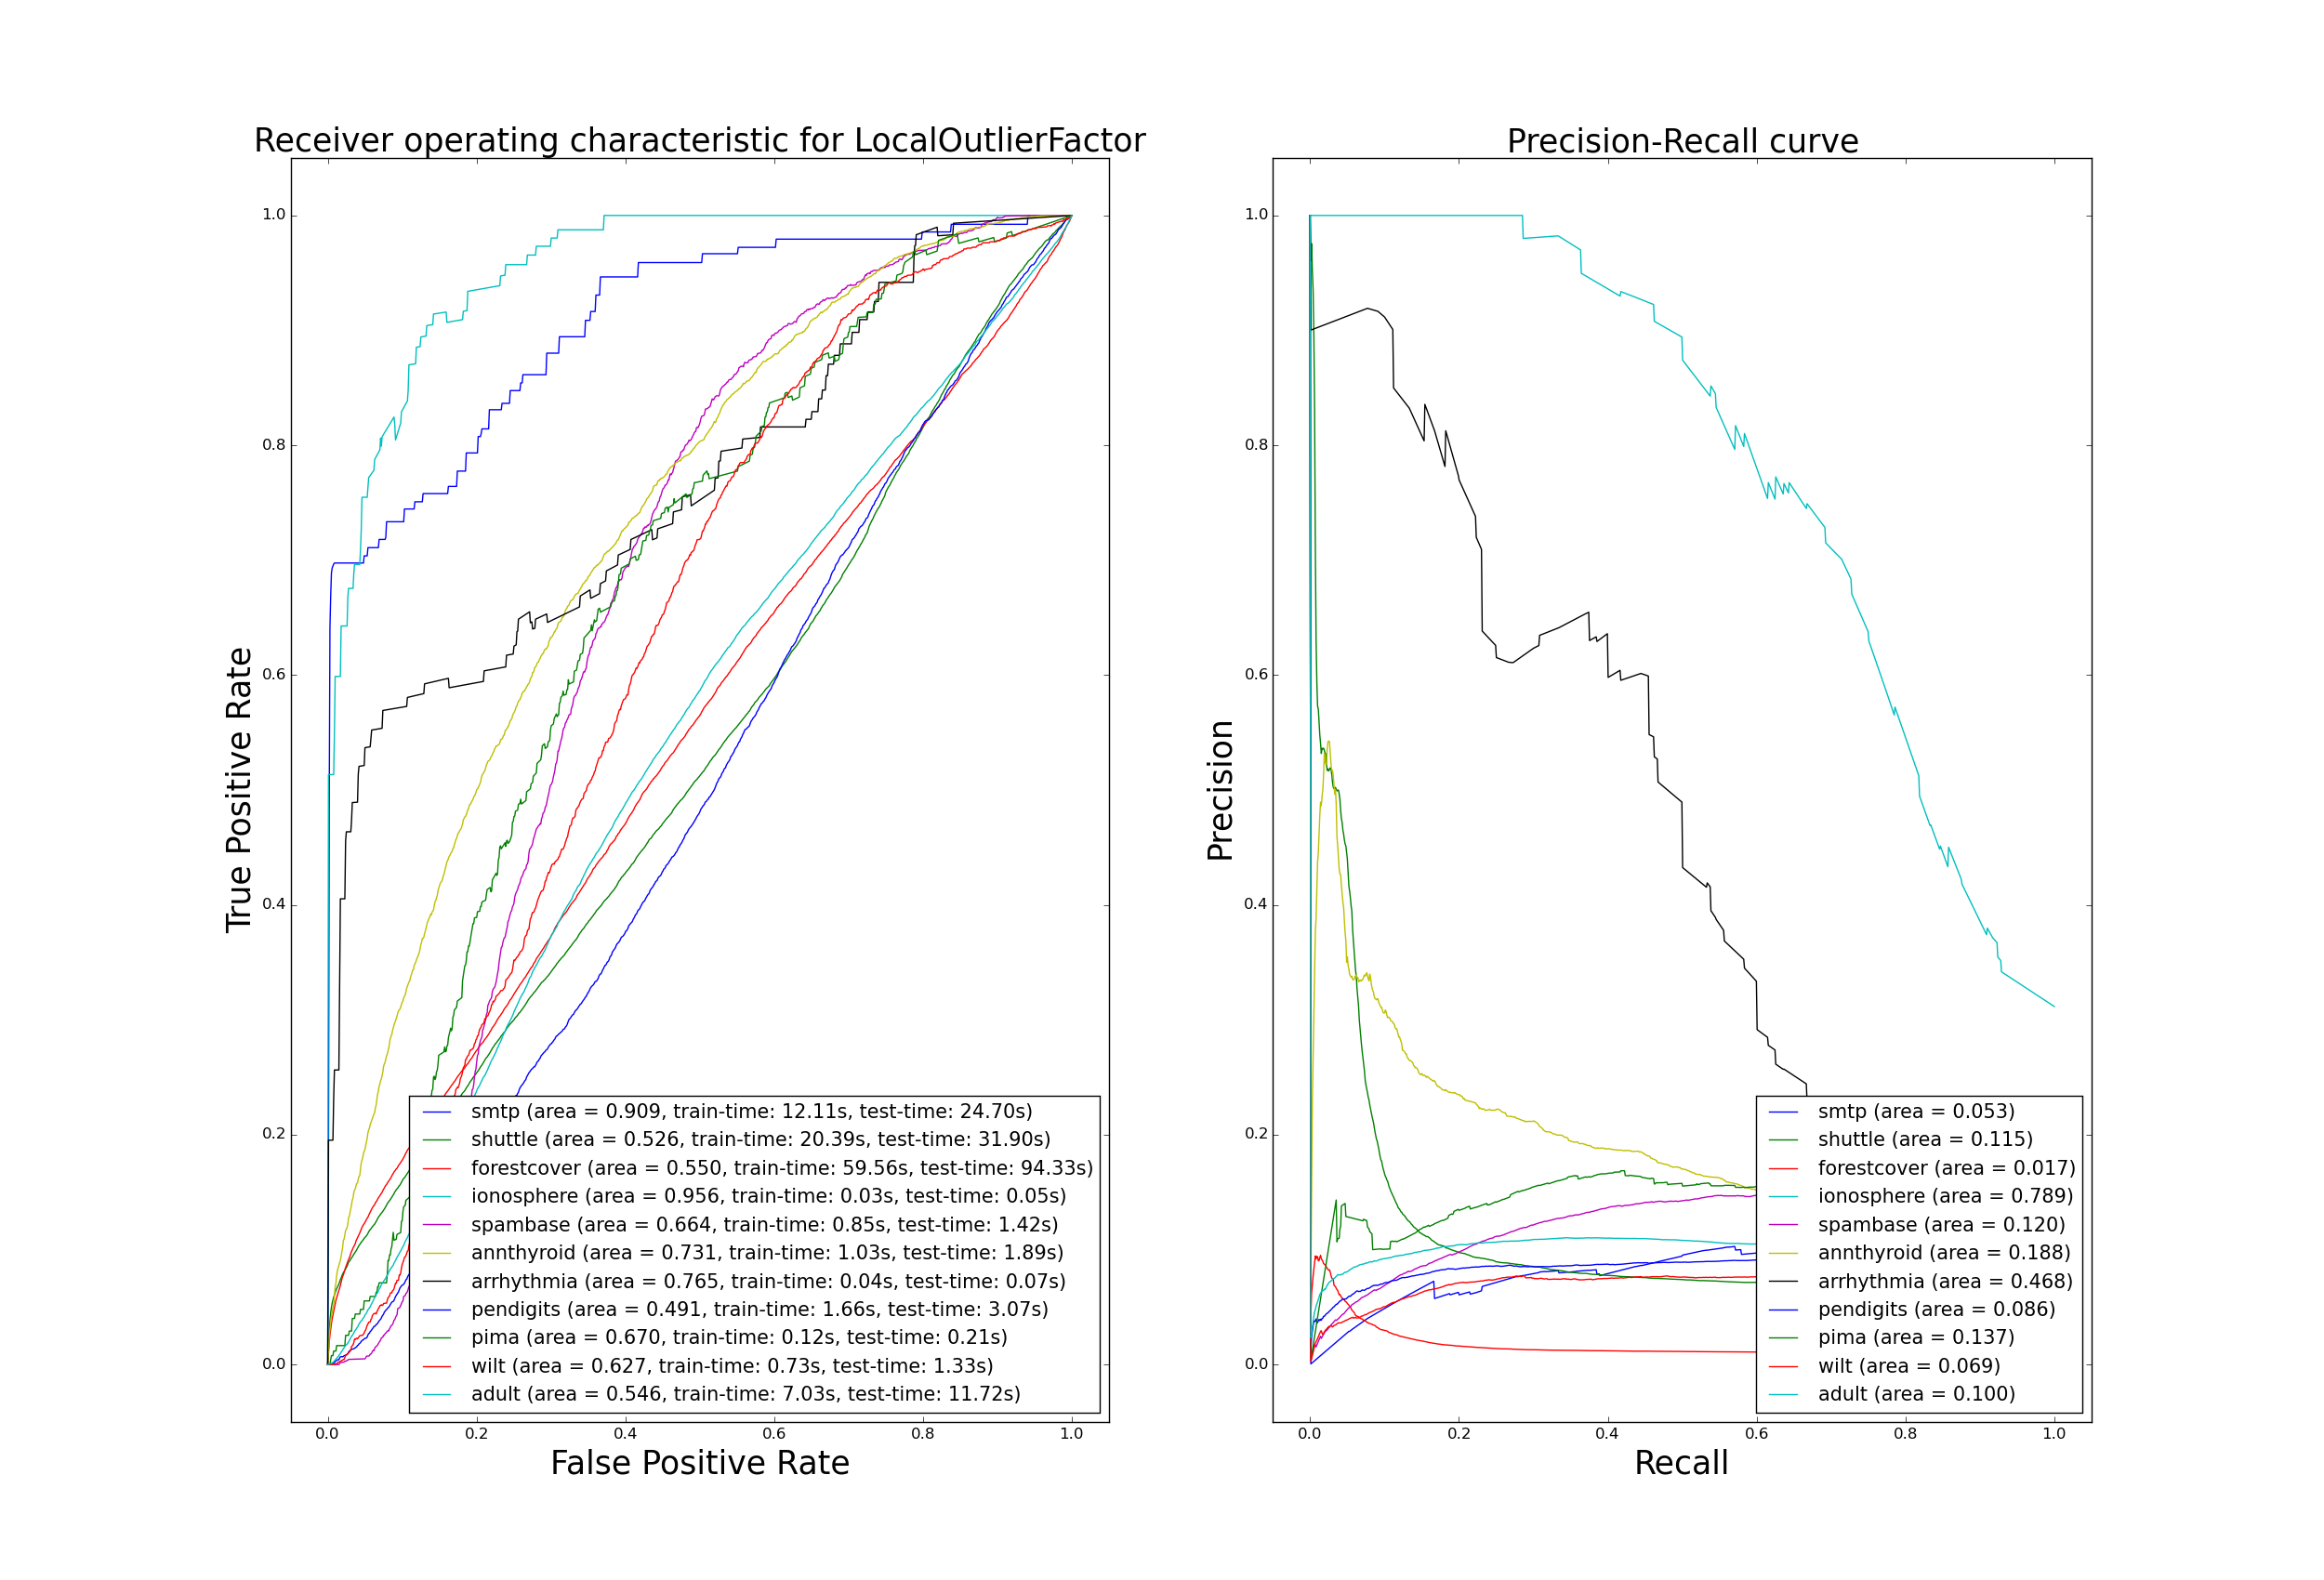
\includegraphics[trim=175 80 175 123, clip, width=\linewidth]{fig_source/ocrf_fig/bench_lof_roc_pr_unsupervised_factorized.png}
\end{figure}

\begin{figure}[!ht]
  \caption{ROC and PR curves for Orca (novelty detection framework)}
  \label{ocrf:fig:orca_roc_pr}
  \centering
  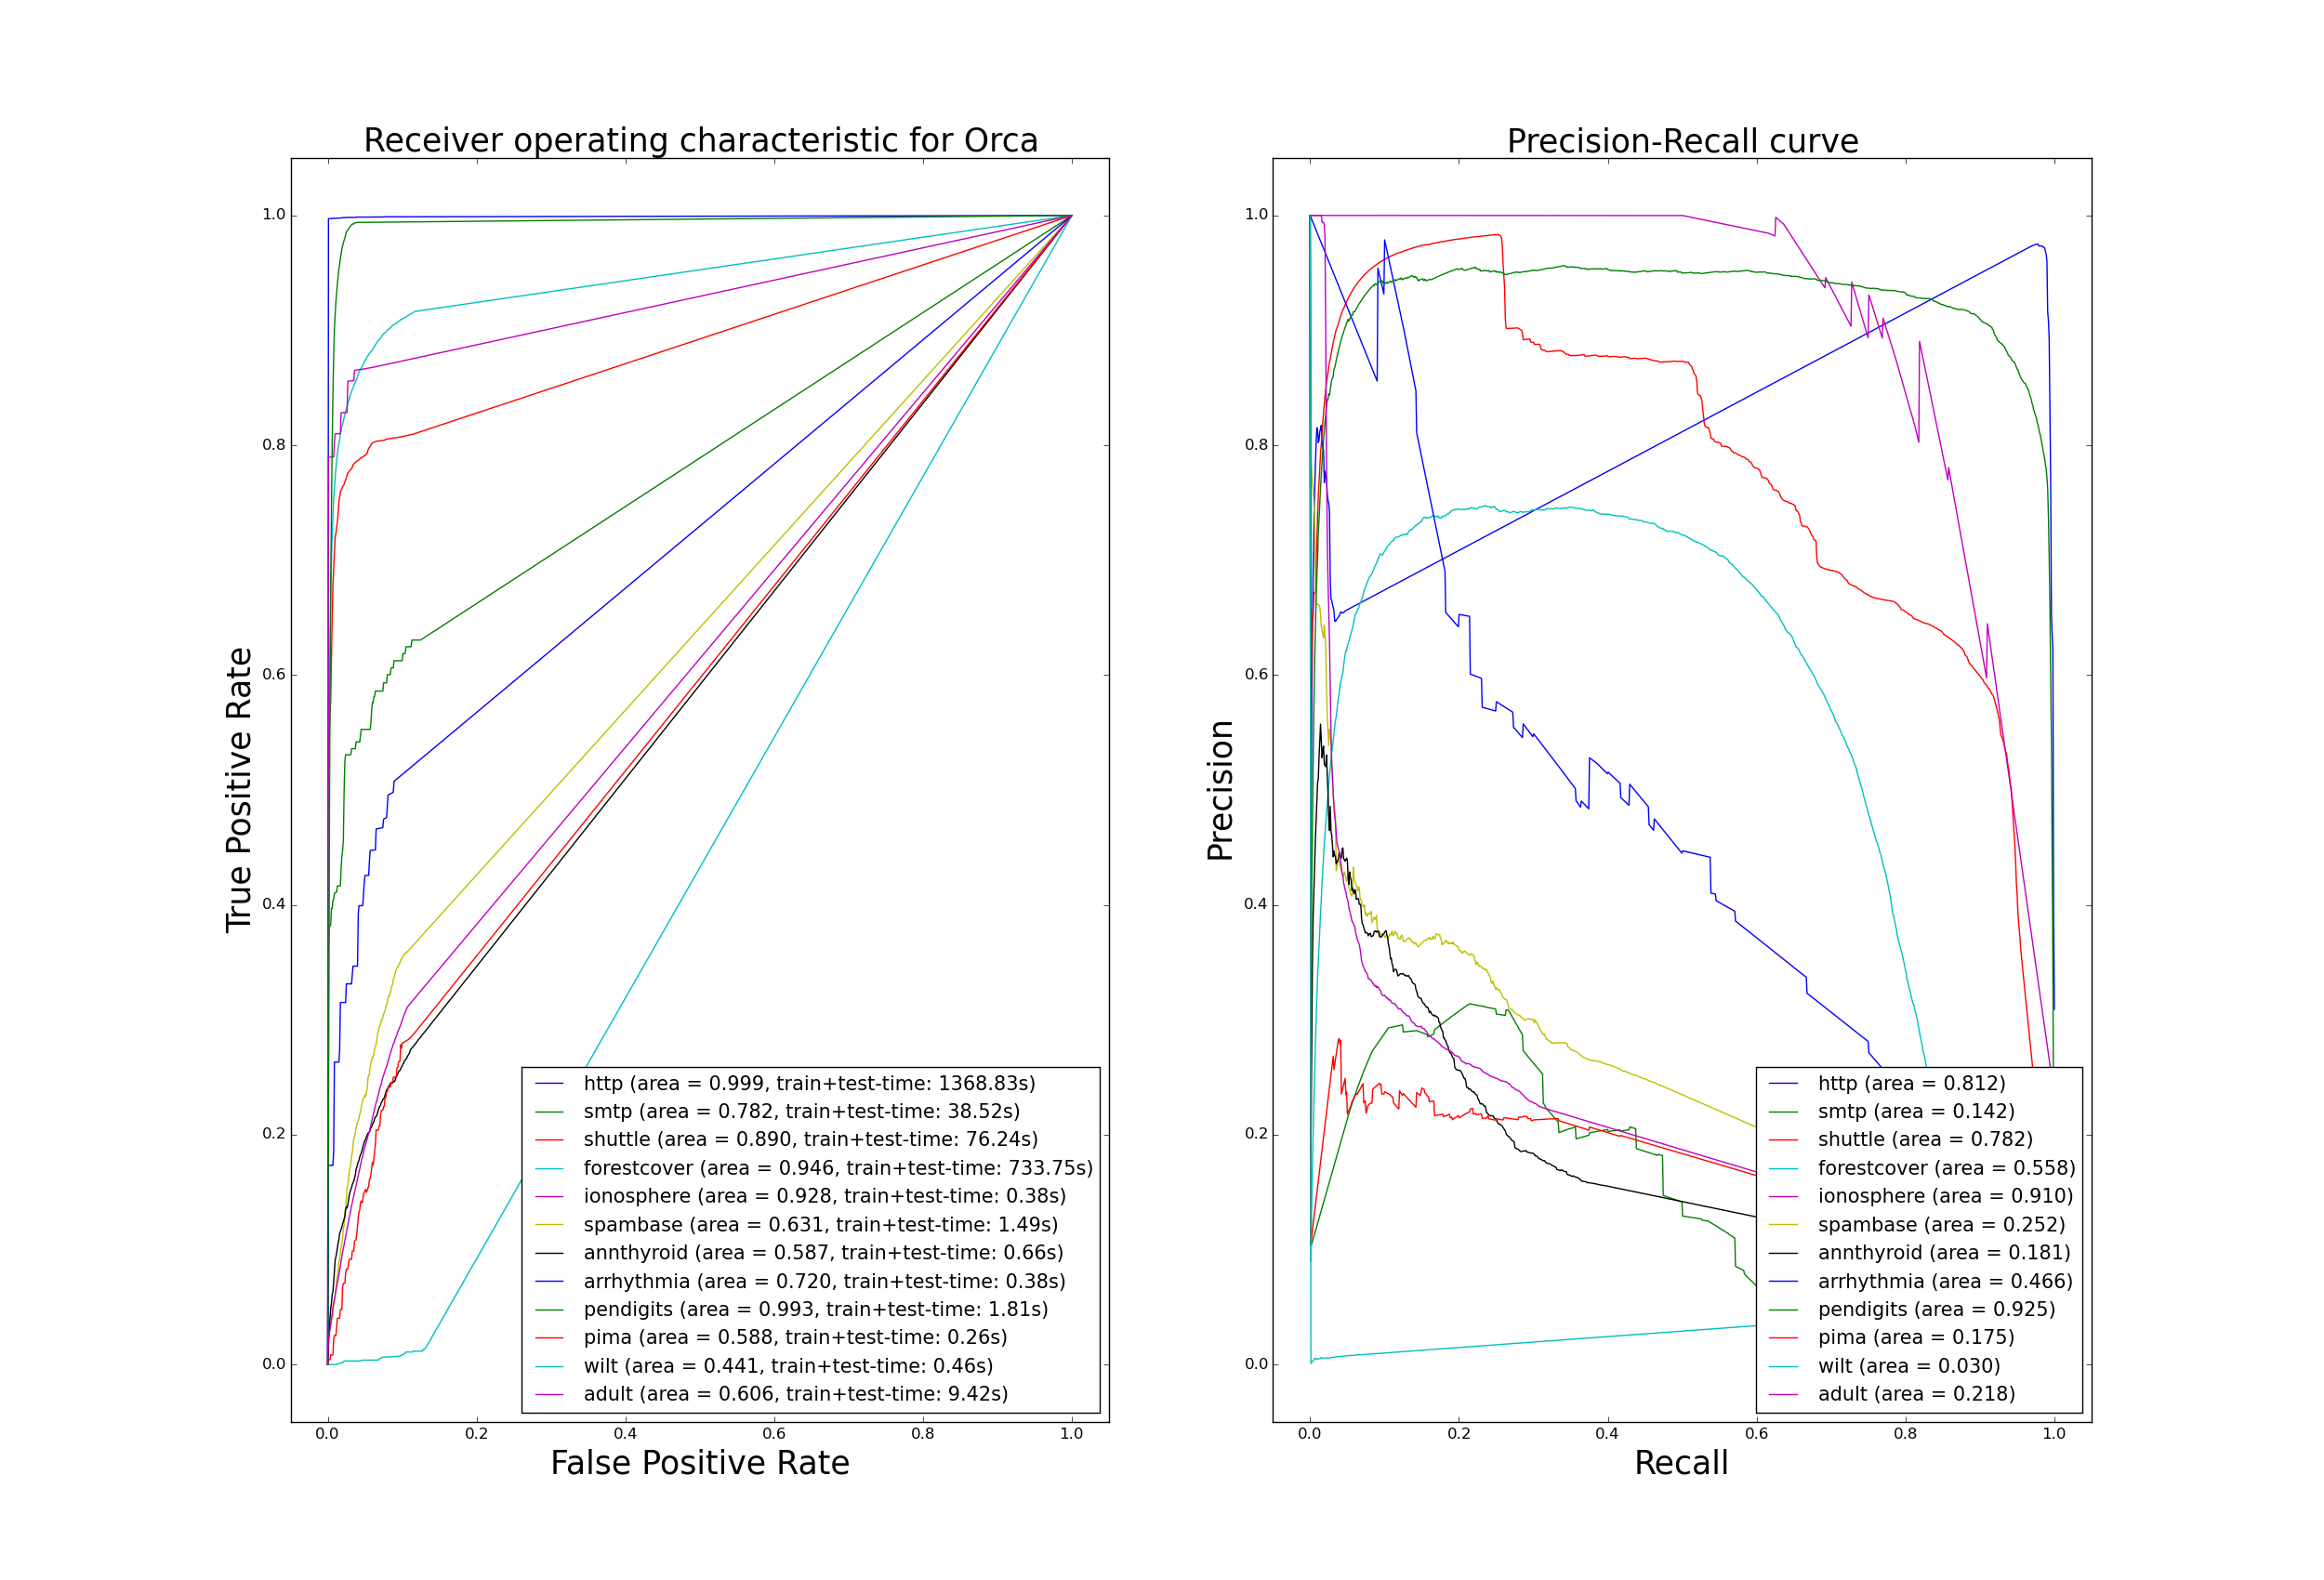
\includegraphics[trim=175 80 175 123, clip, width=\linewidth]{fig_source/ocrf_fig/bench_orca_roc_pr_supervised_factorized.png}
\end{figure}
\begin{figure}[!ht]
  \caption{ROC and PR curves for Orca (unsupervised framework)}
  \label{ocrf:fig:orca_roc_pr_unsupervised}
  \centering
  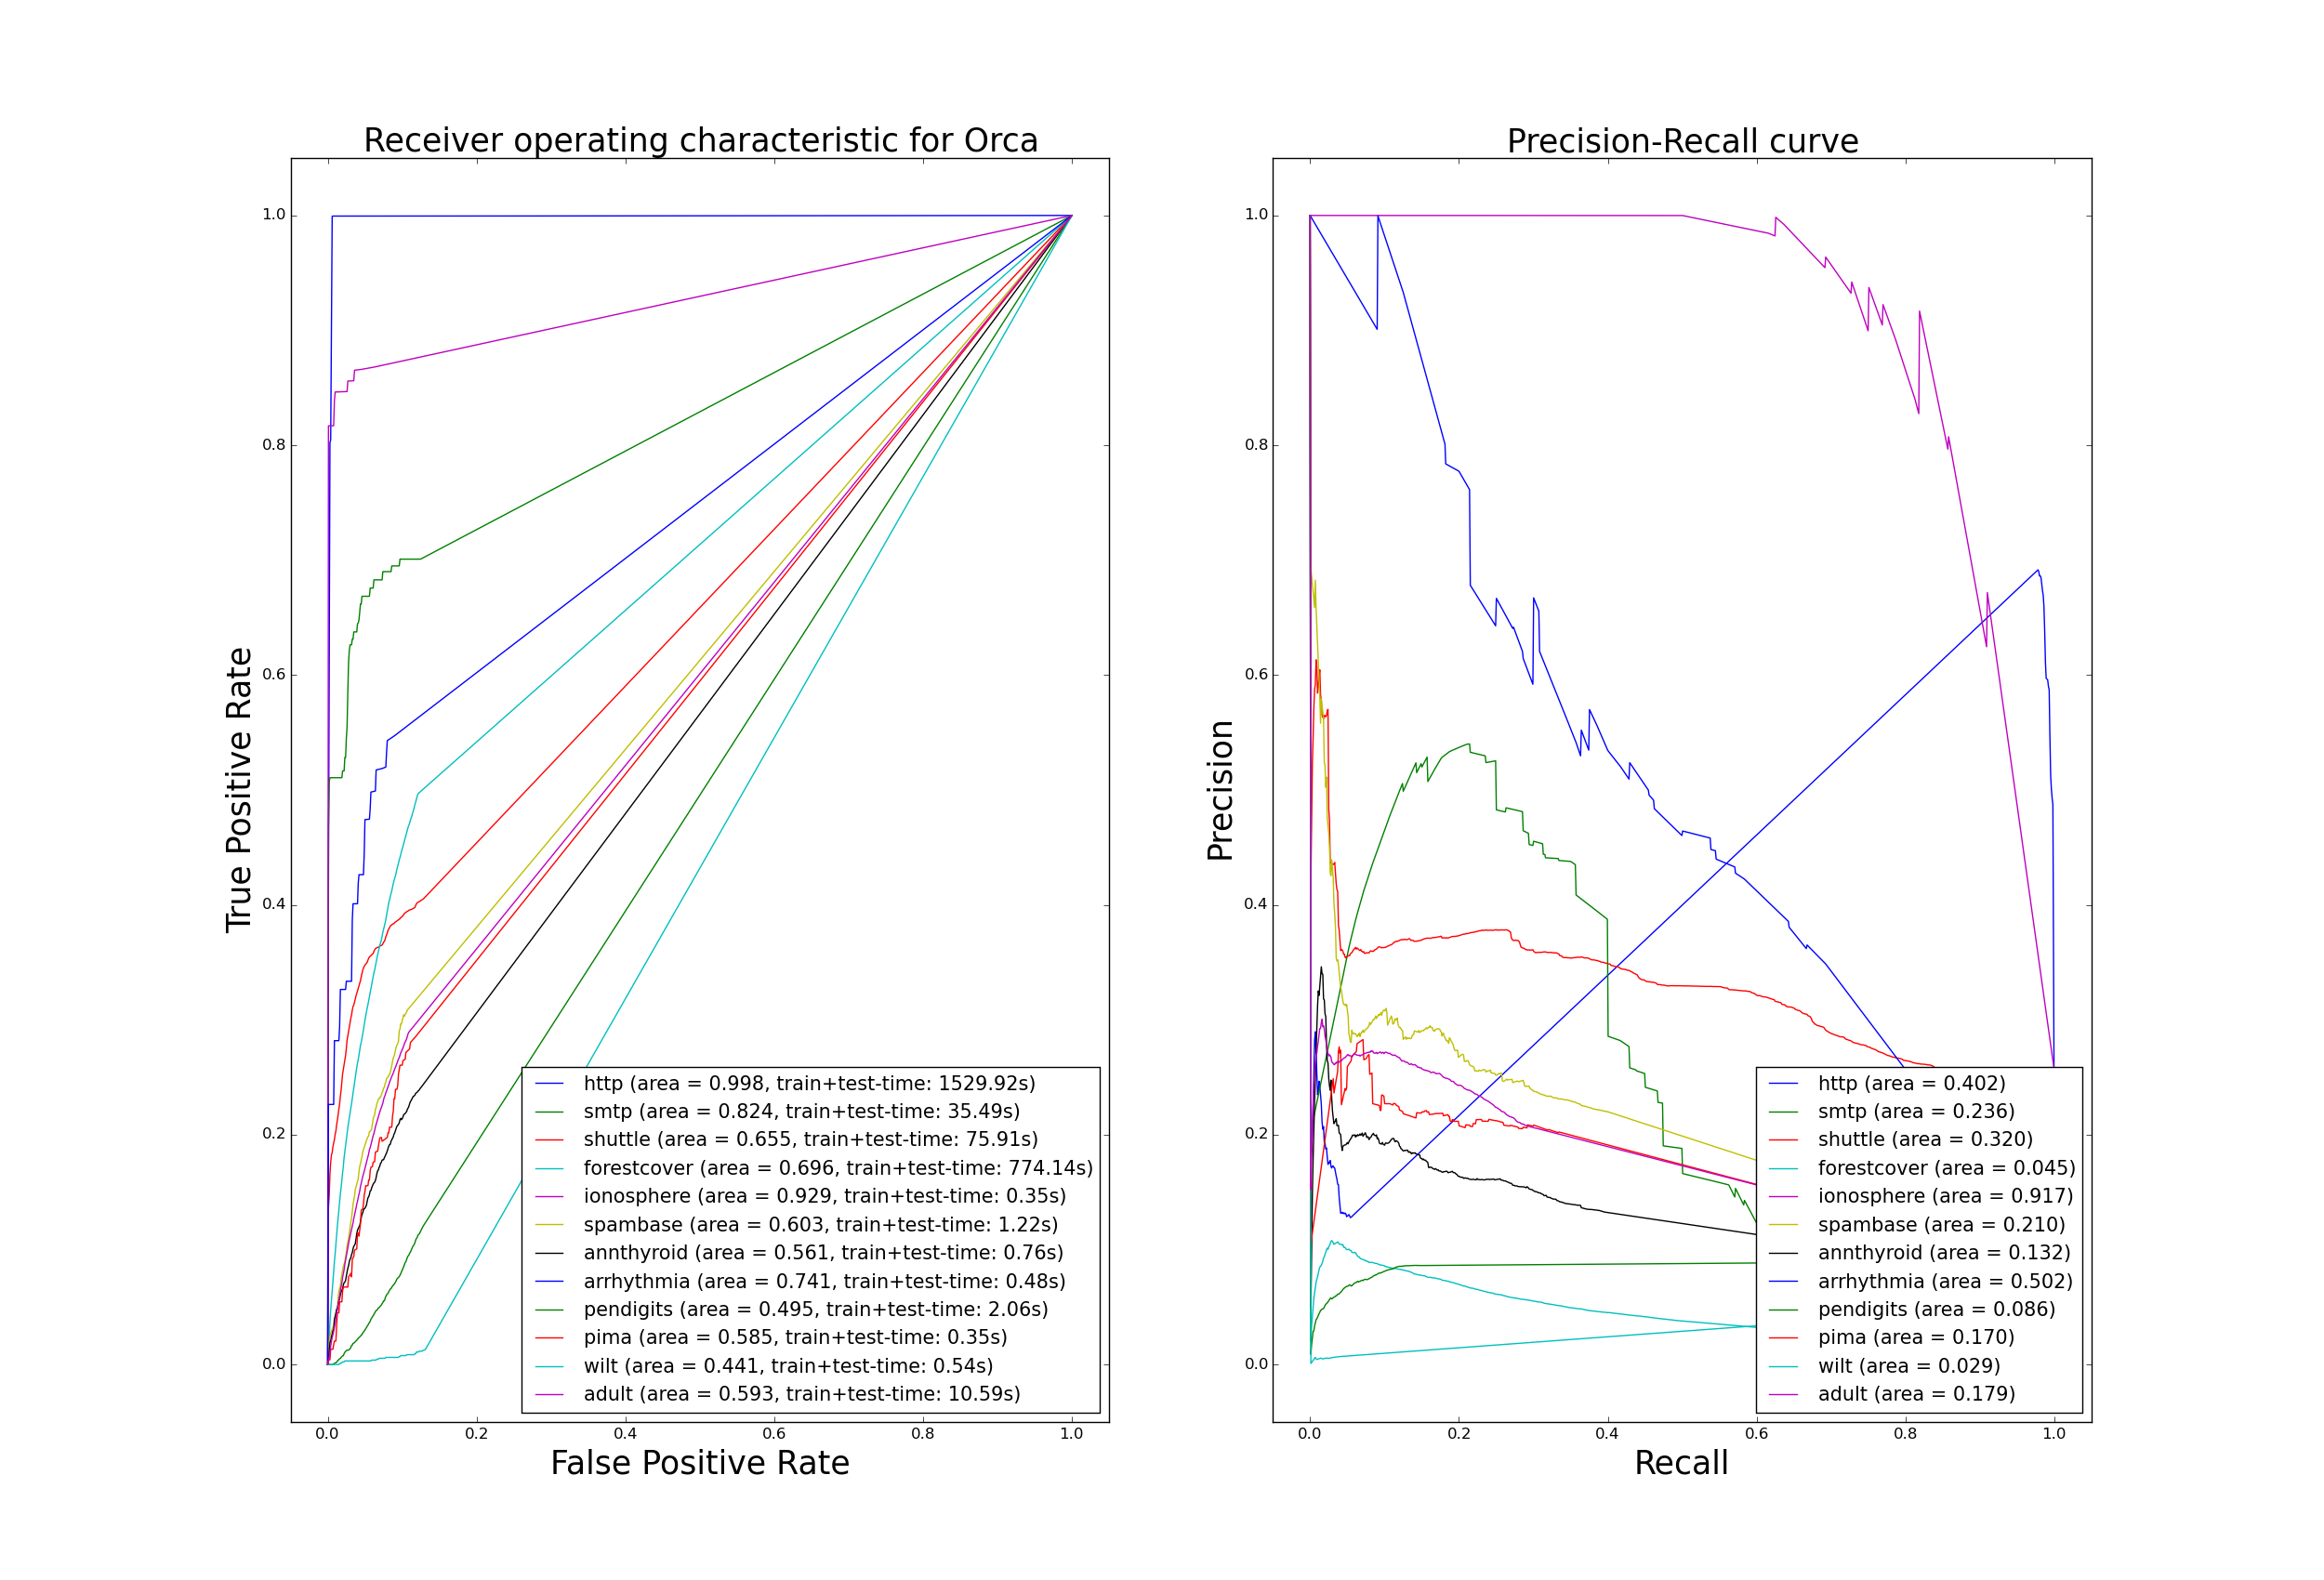
\includegraphics[trim=175 80 175 123, clip, width=\linewidth]{fig_source/ocrf_fig/bench_orca_roc_pr_unsupervised_factorized.png}
\end{figure}

\begin{figure}[!ht]
  \caption{ROC and PR curves for LSAD (novelty detection framework)}
  \label{ocrf:fig:LSAnomaly_roc_pr}
  \centering
  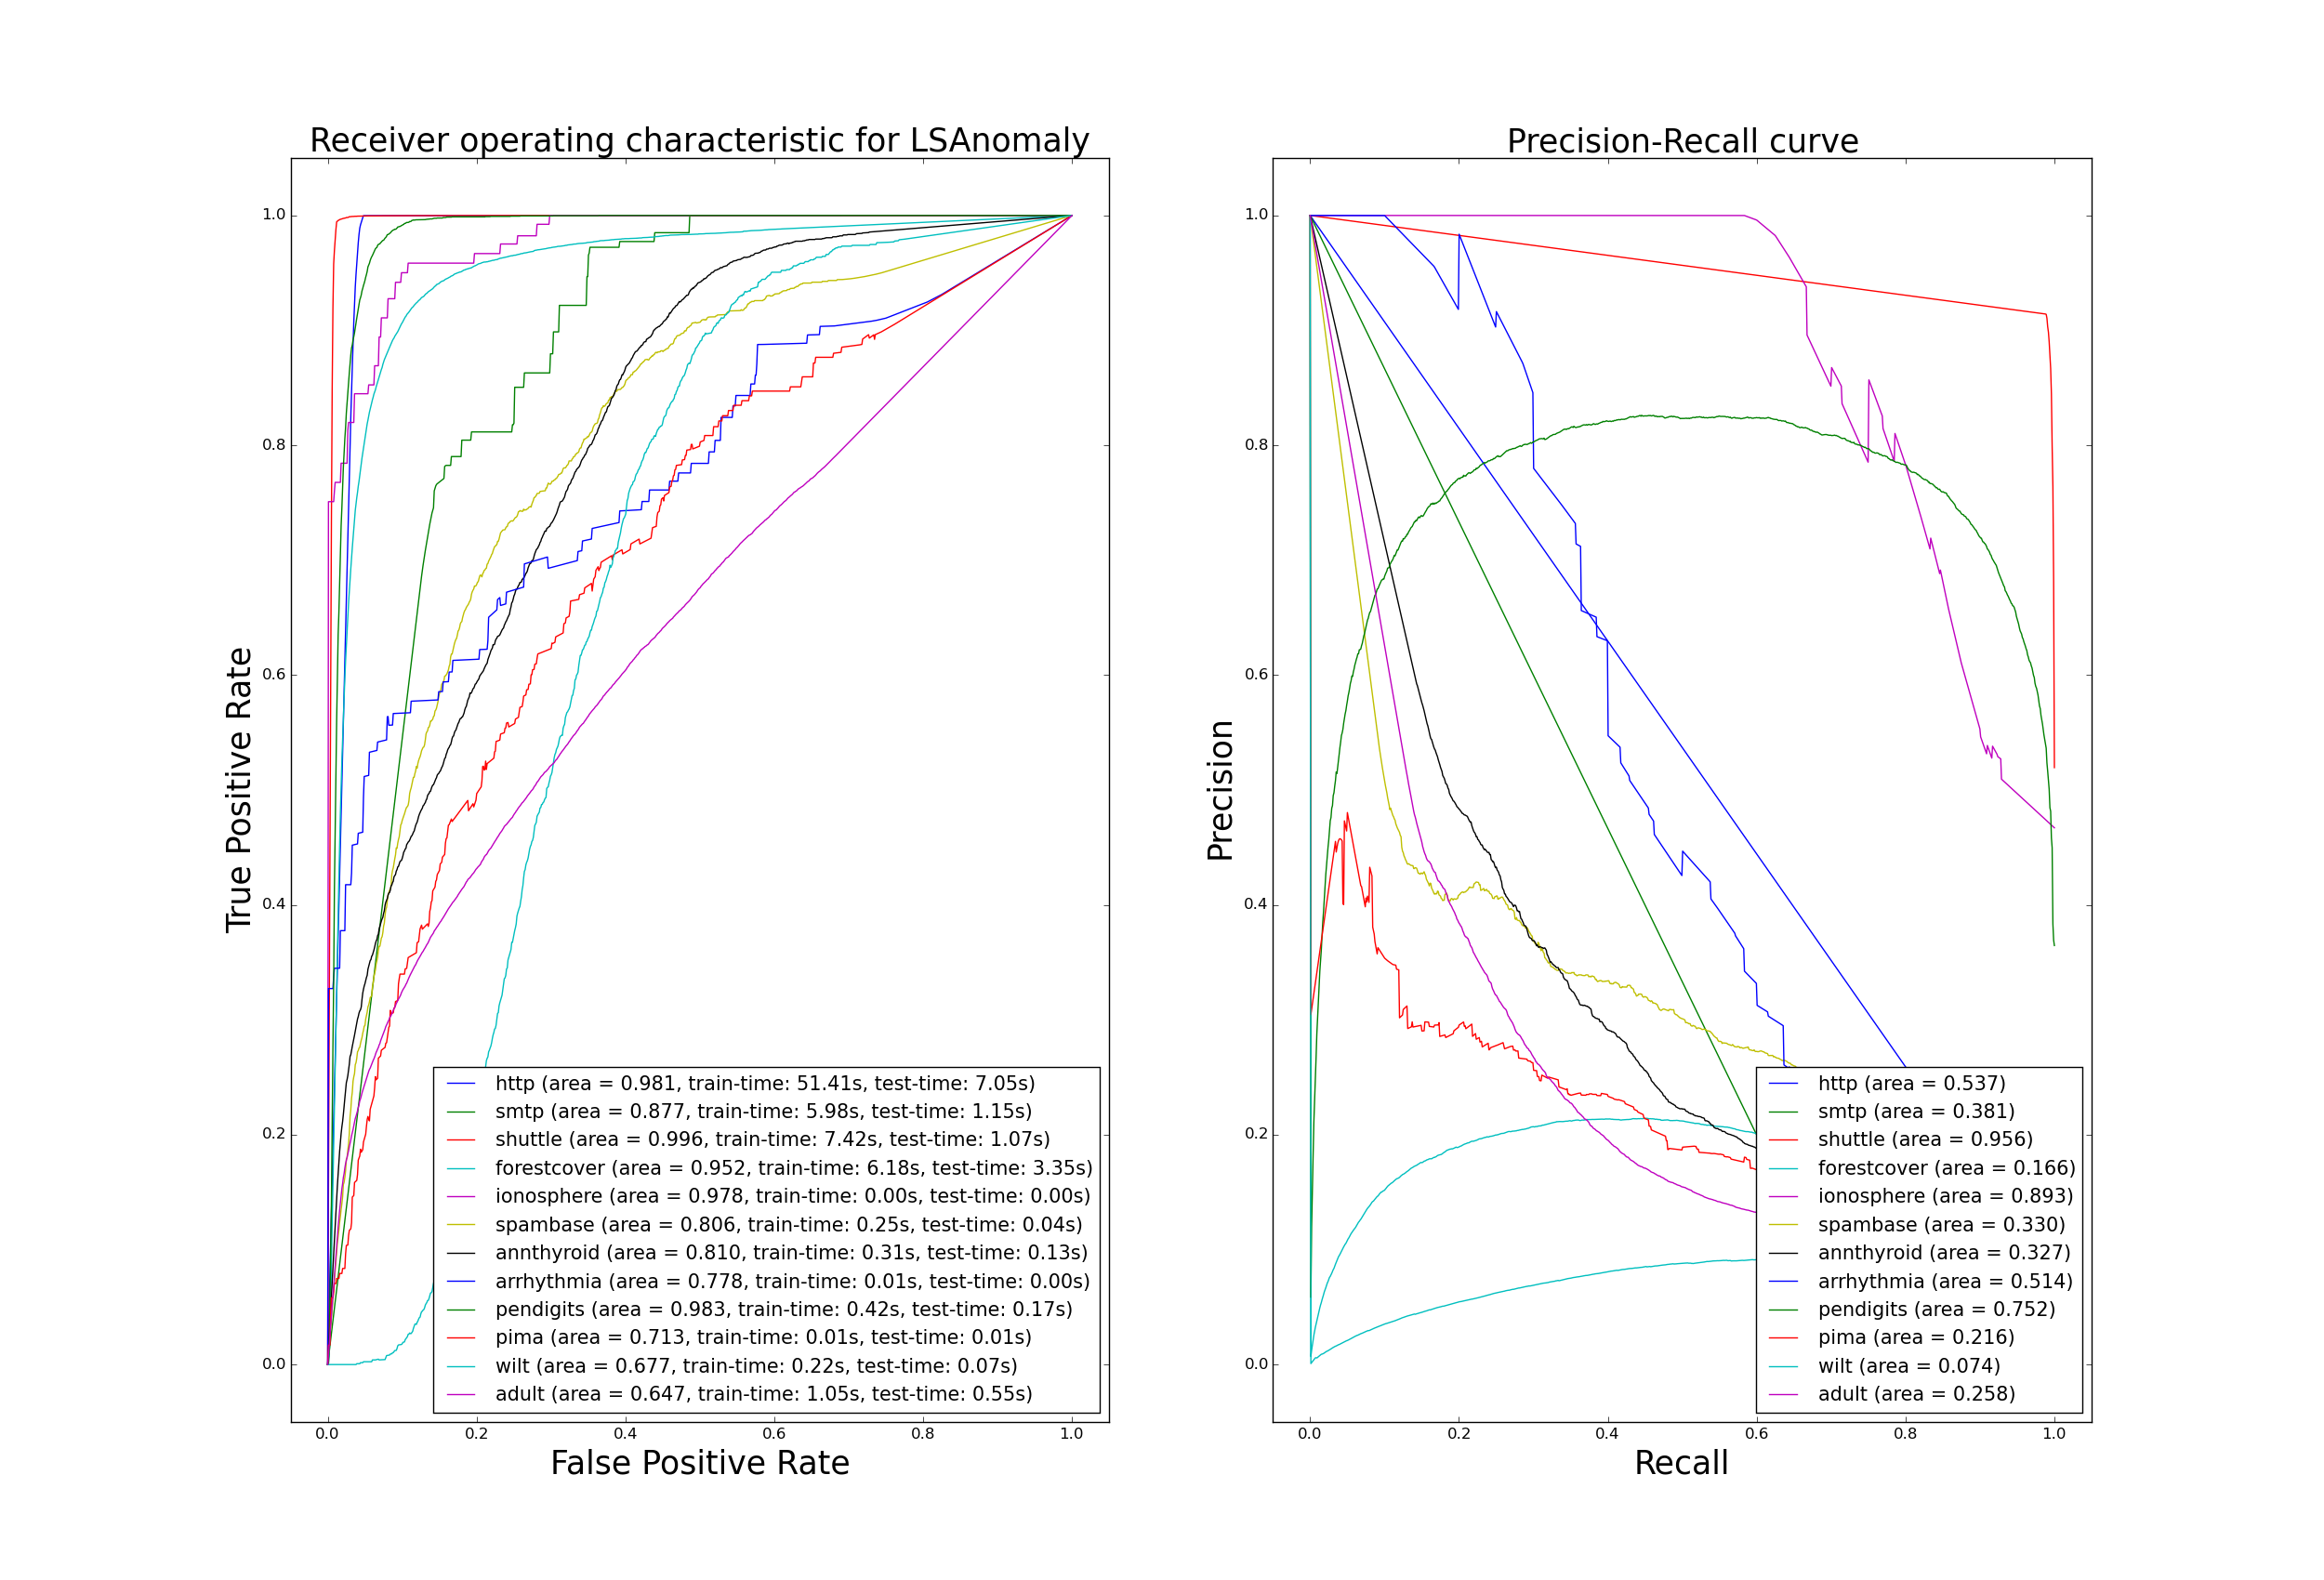
\includegraphics[trim=175 80 175 123, clip, width=\linewidth]{fig_source/ocrf_fig/bench_LSAnomaly_roc_pr_supervised_factorized.png}
\end{figure}
\begin{figure}[!ht]
  \caption{ROC and PR curves for LSAD (unsupervised framework)}
  \label{ocrf:fig:LSAnomaly_roc_pr_unsupervised}
  \centering
  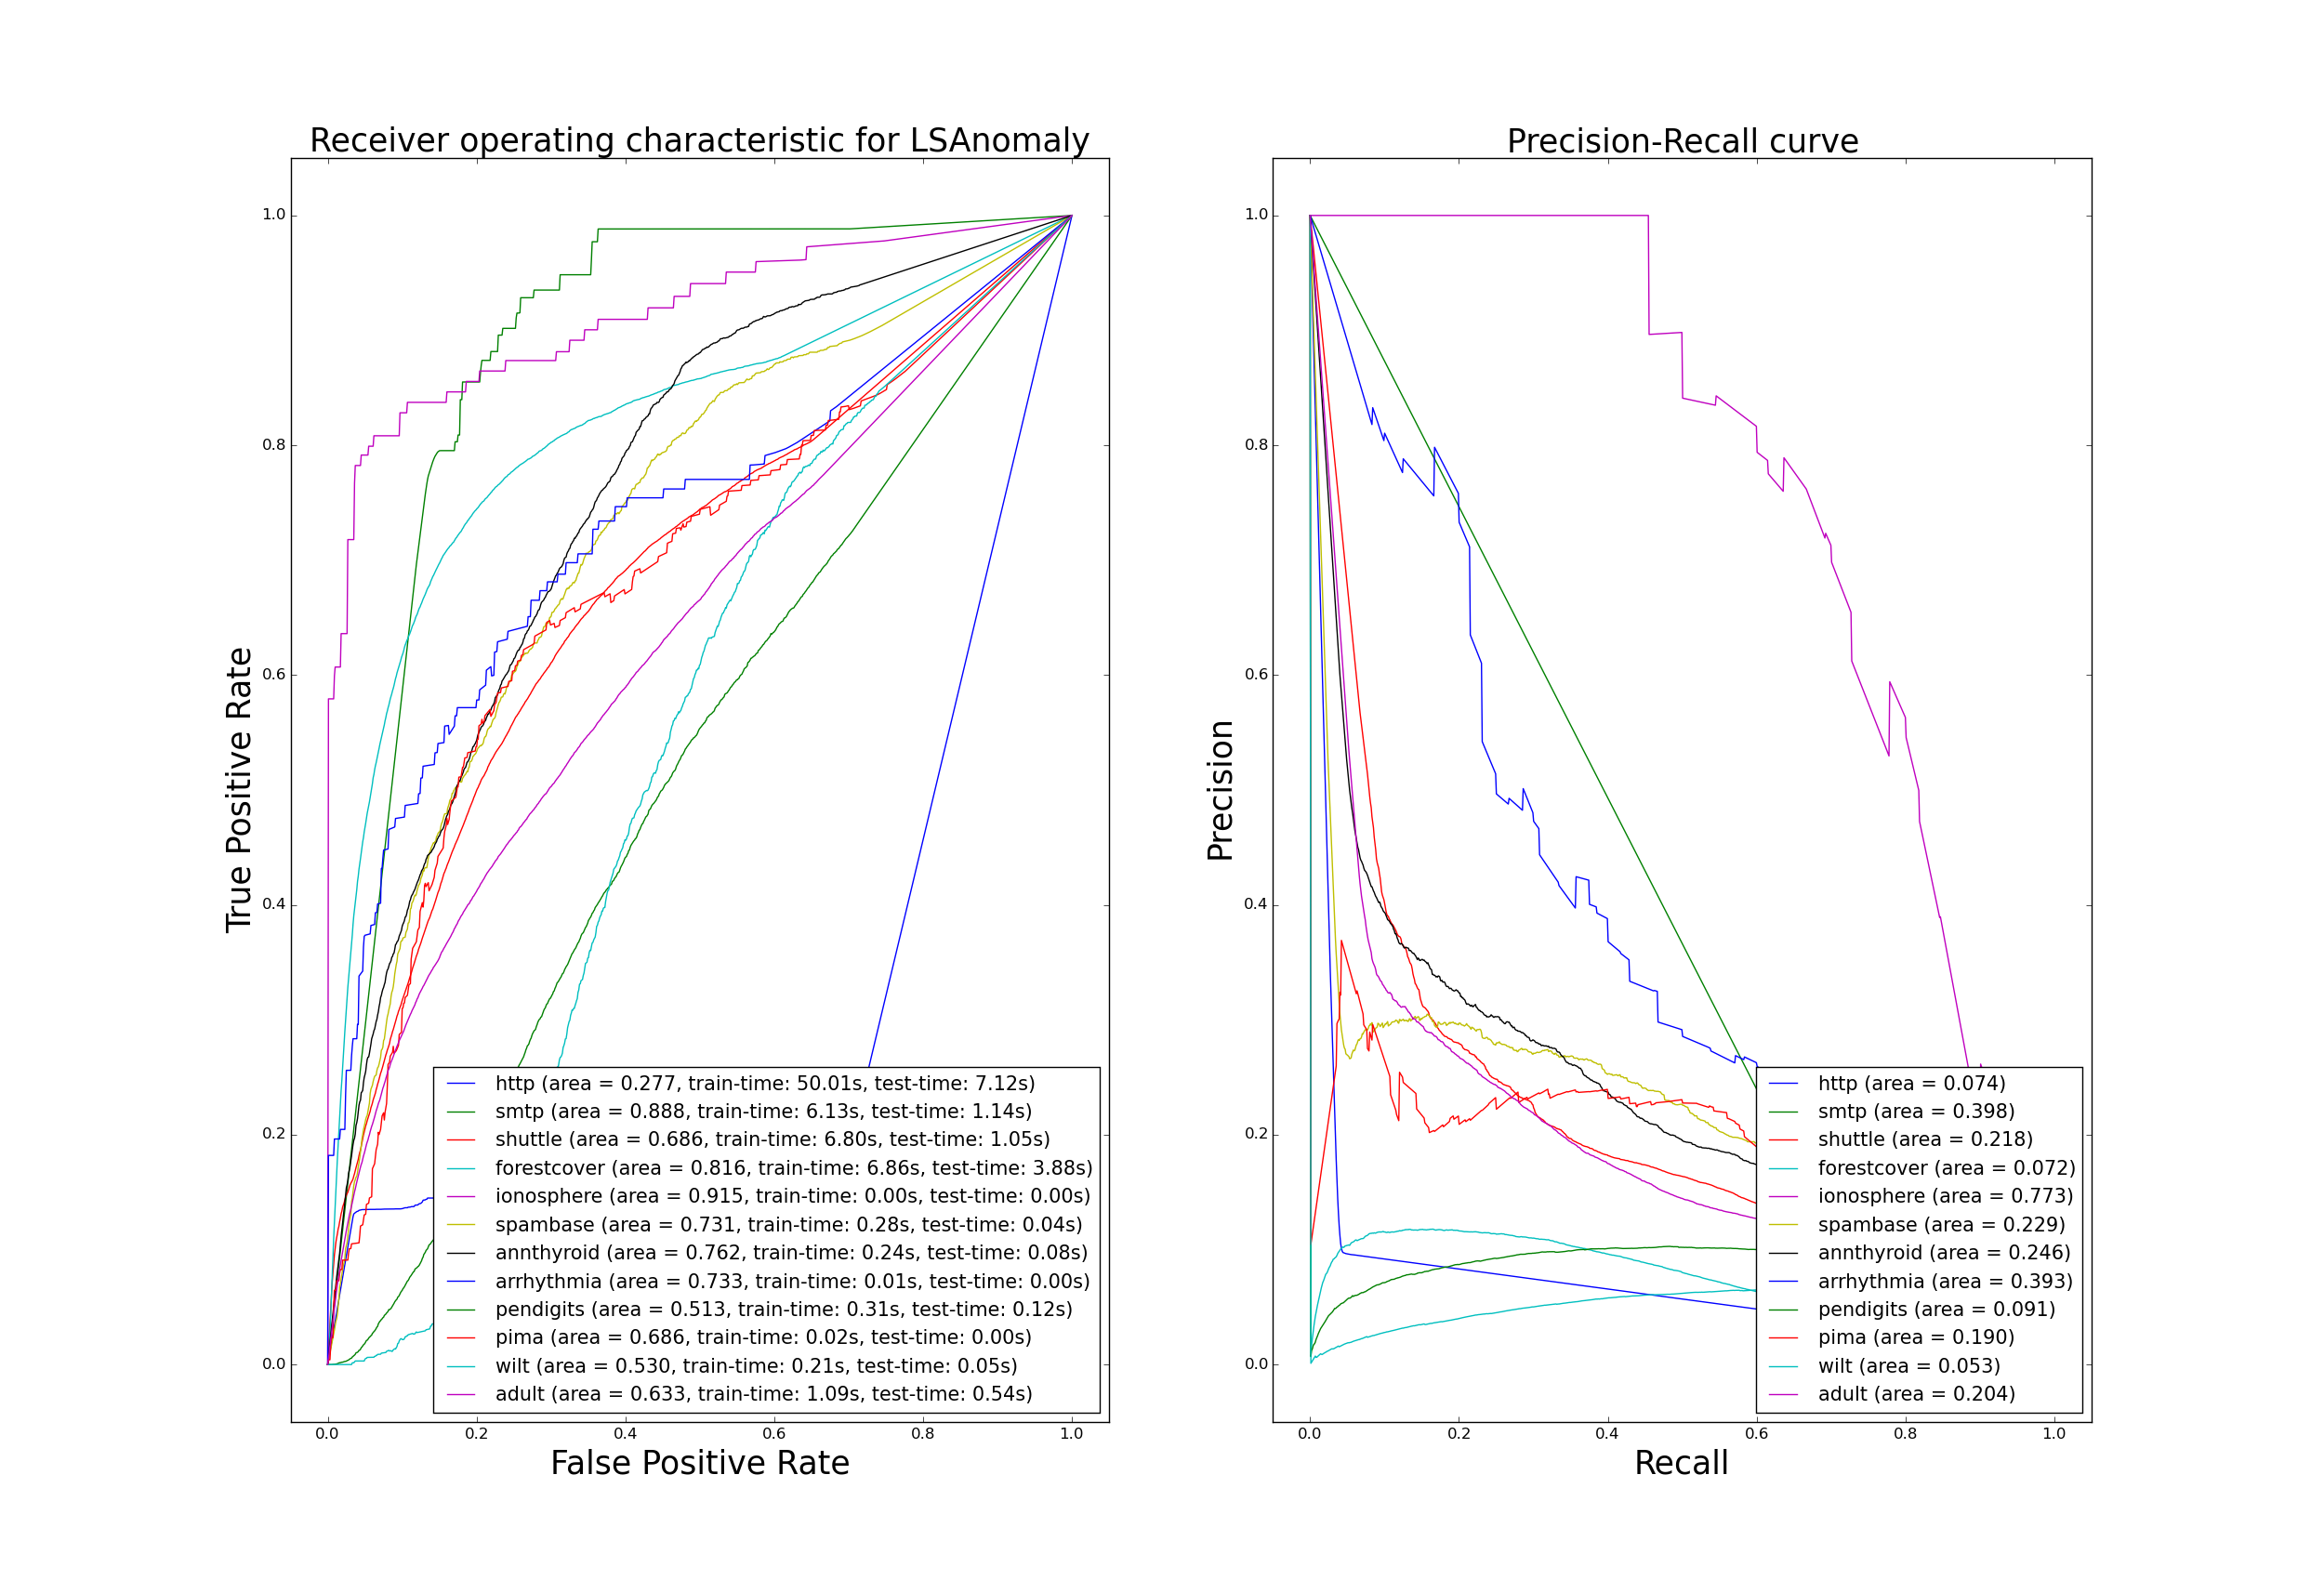
\includegraphics[trim=175 80 175 123, clip, width=\linewidth]{fig_source/ocrf_fig/bench_LSAnomaly_roc_pr_unsupervised_factorized.png}
\end{figure}

\begin{figure}[!ht]
  \caption{ROC and PR curves for RFC (novelty detection framework)}
  \label{ocrf:fig:rf_roc_pr}
  \centering
  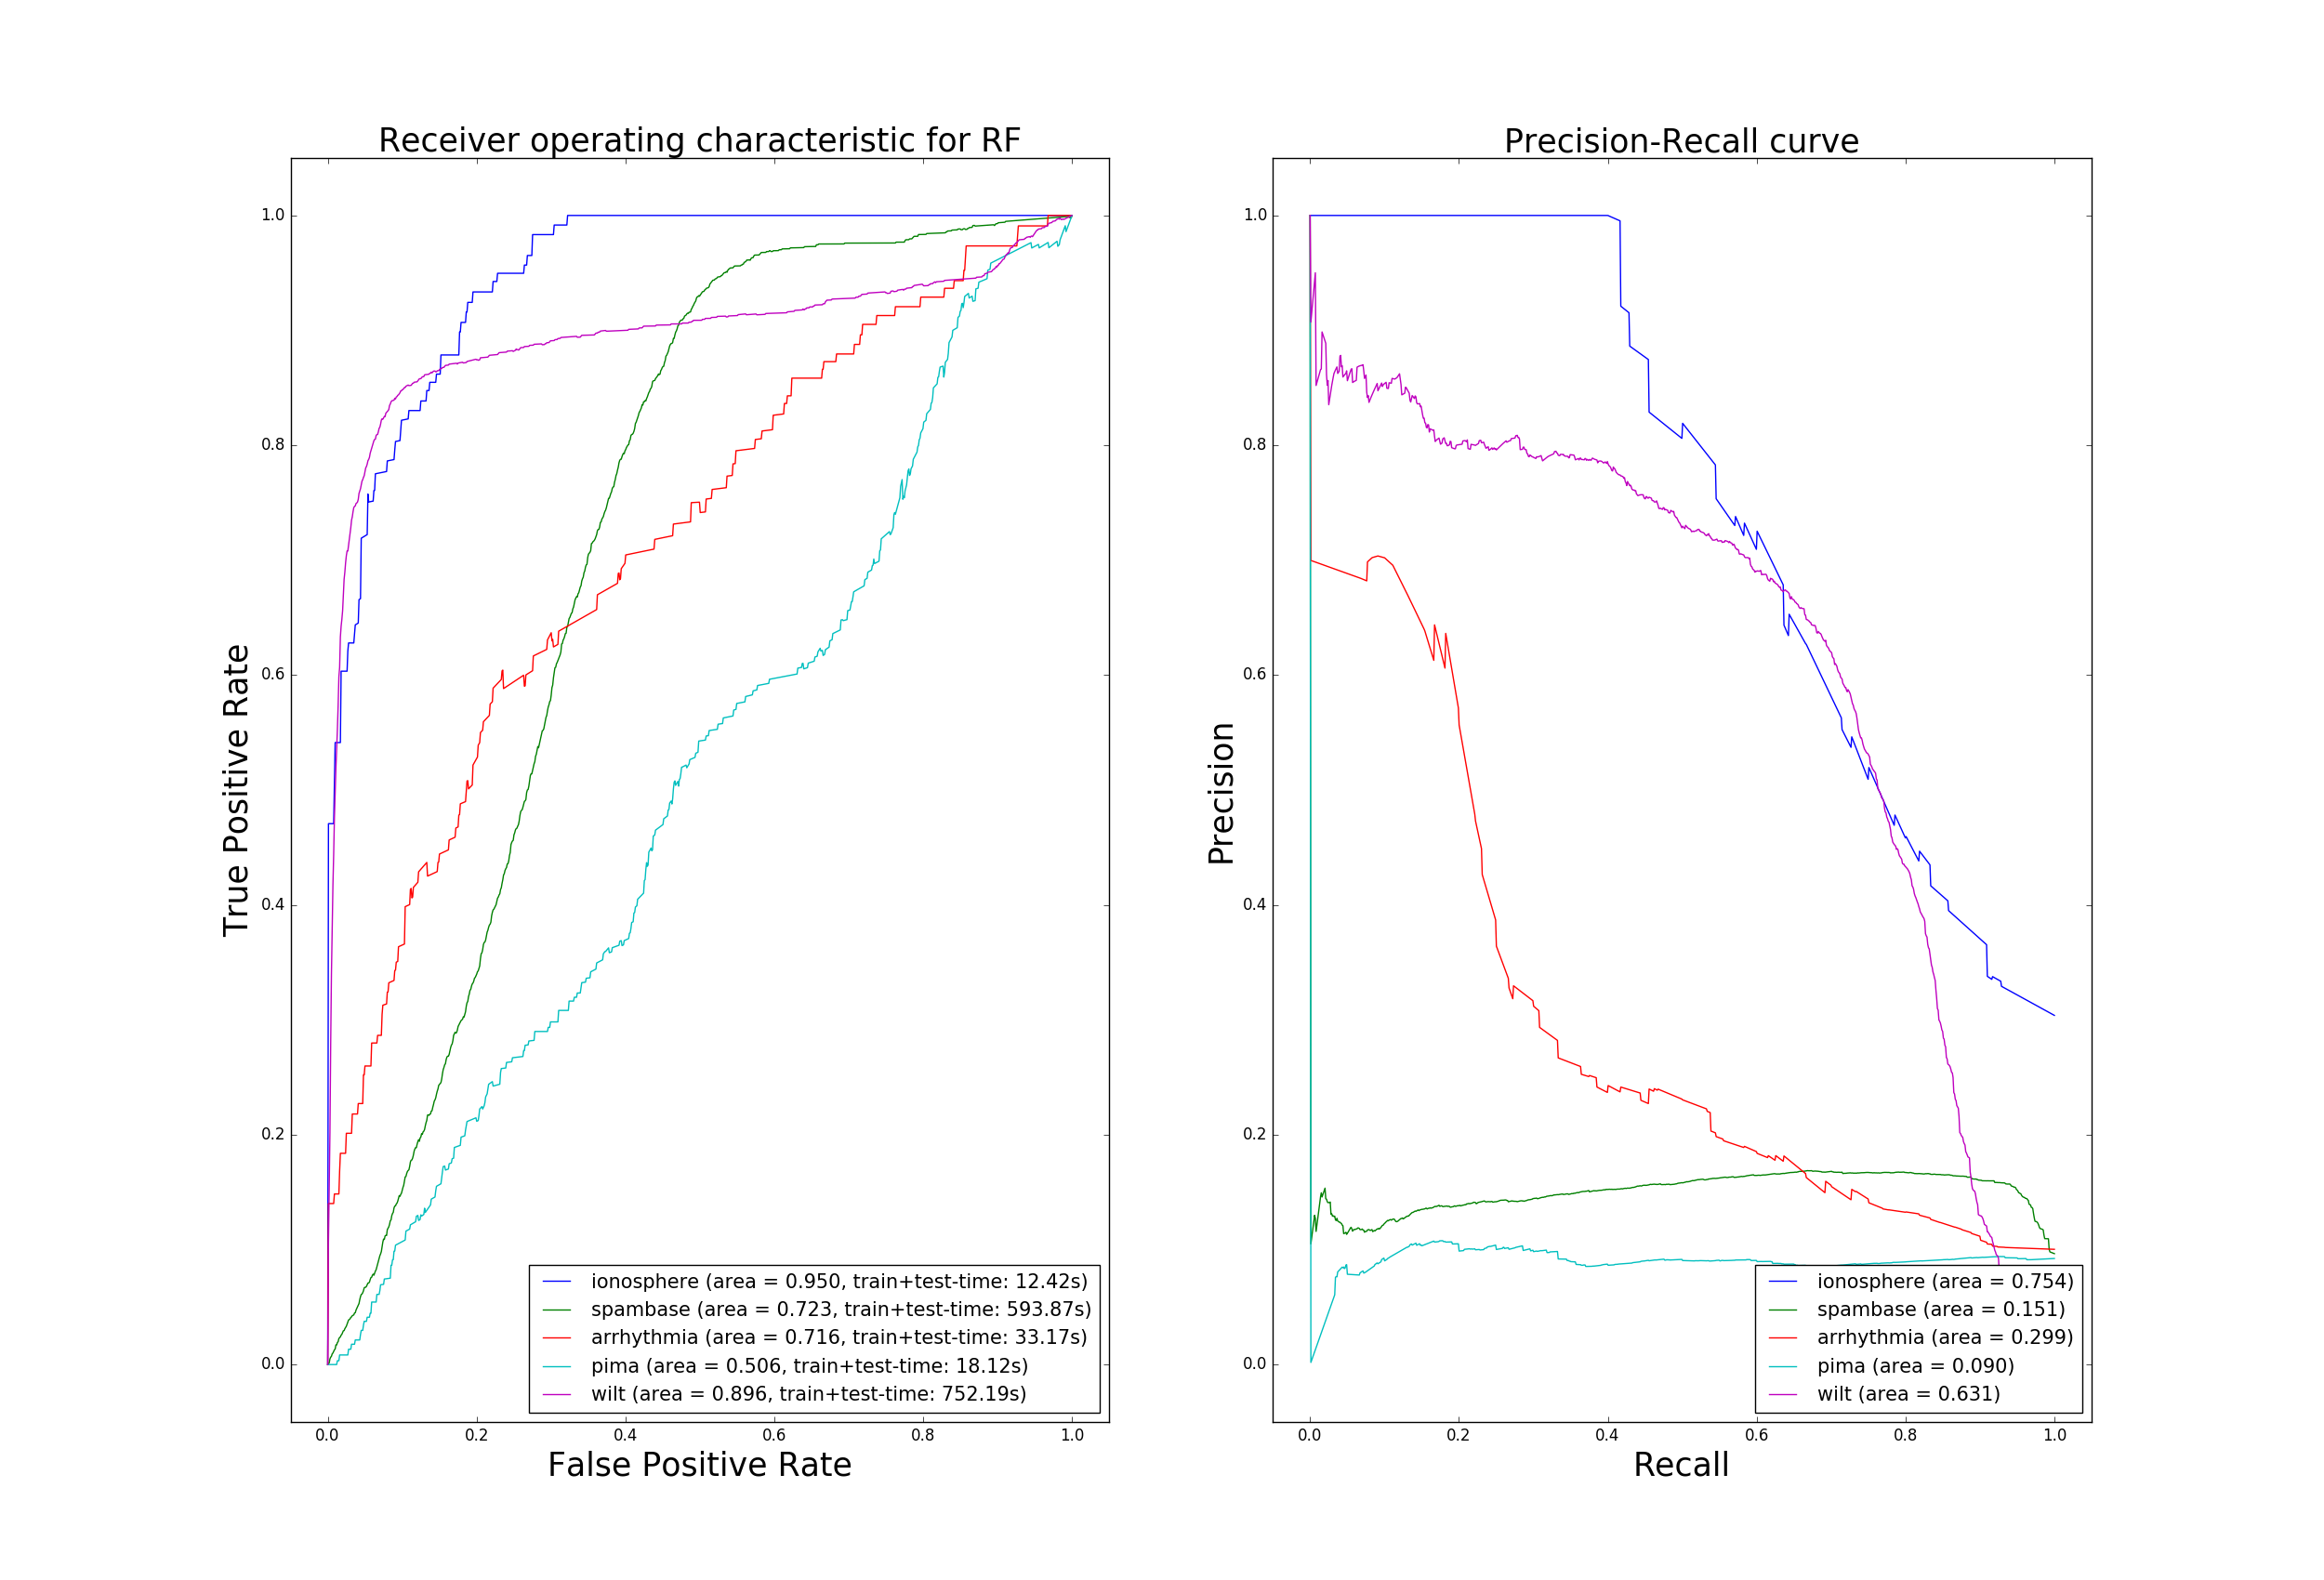
\includegraphics[trim=175 80 175 123, clip, width=\linewidth]{fig_source/ocrf_fig/bench_rf_roc_pr_supervised_factorized.png}
\end{figure}
\begin{figure}[!ht]
  \caption{ROC and PR curves for RFC (unsupervised framework)}
  \label{ocrf:fig:rf_roc_pr_unsupervised}
  \centering
  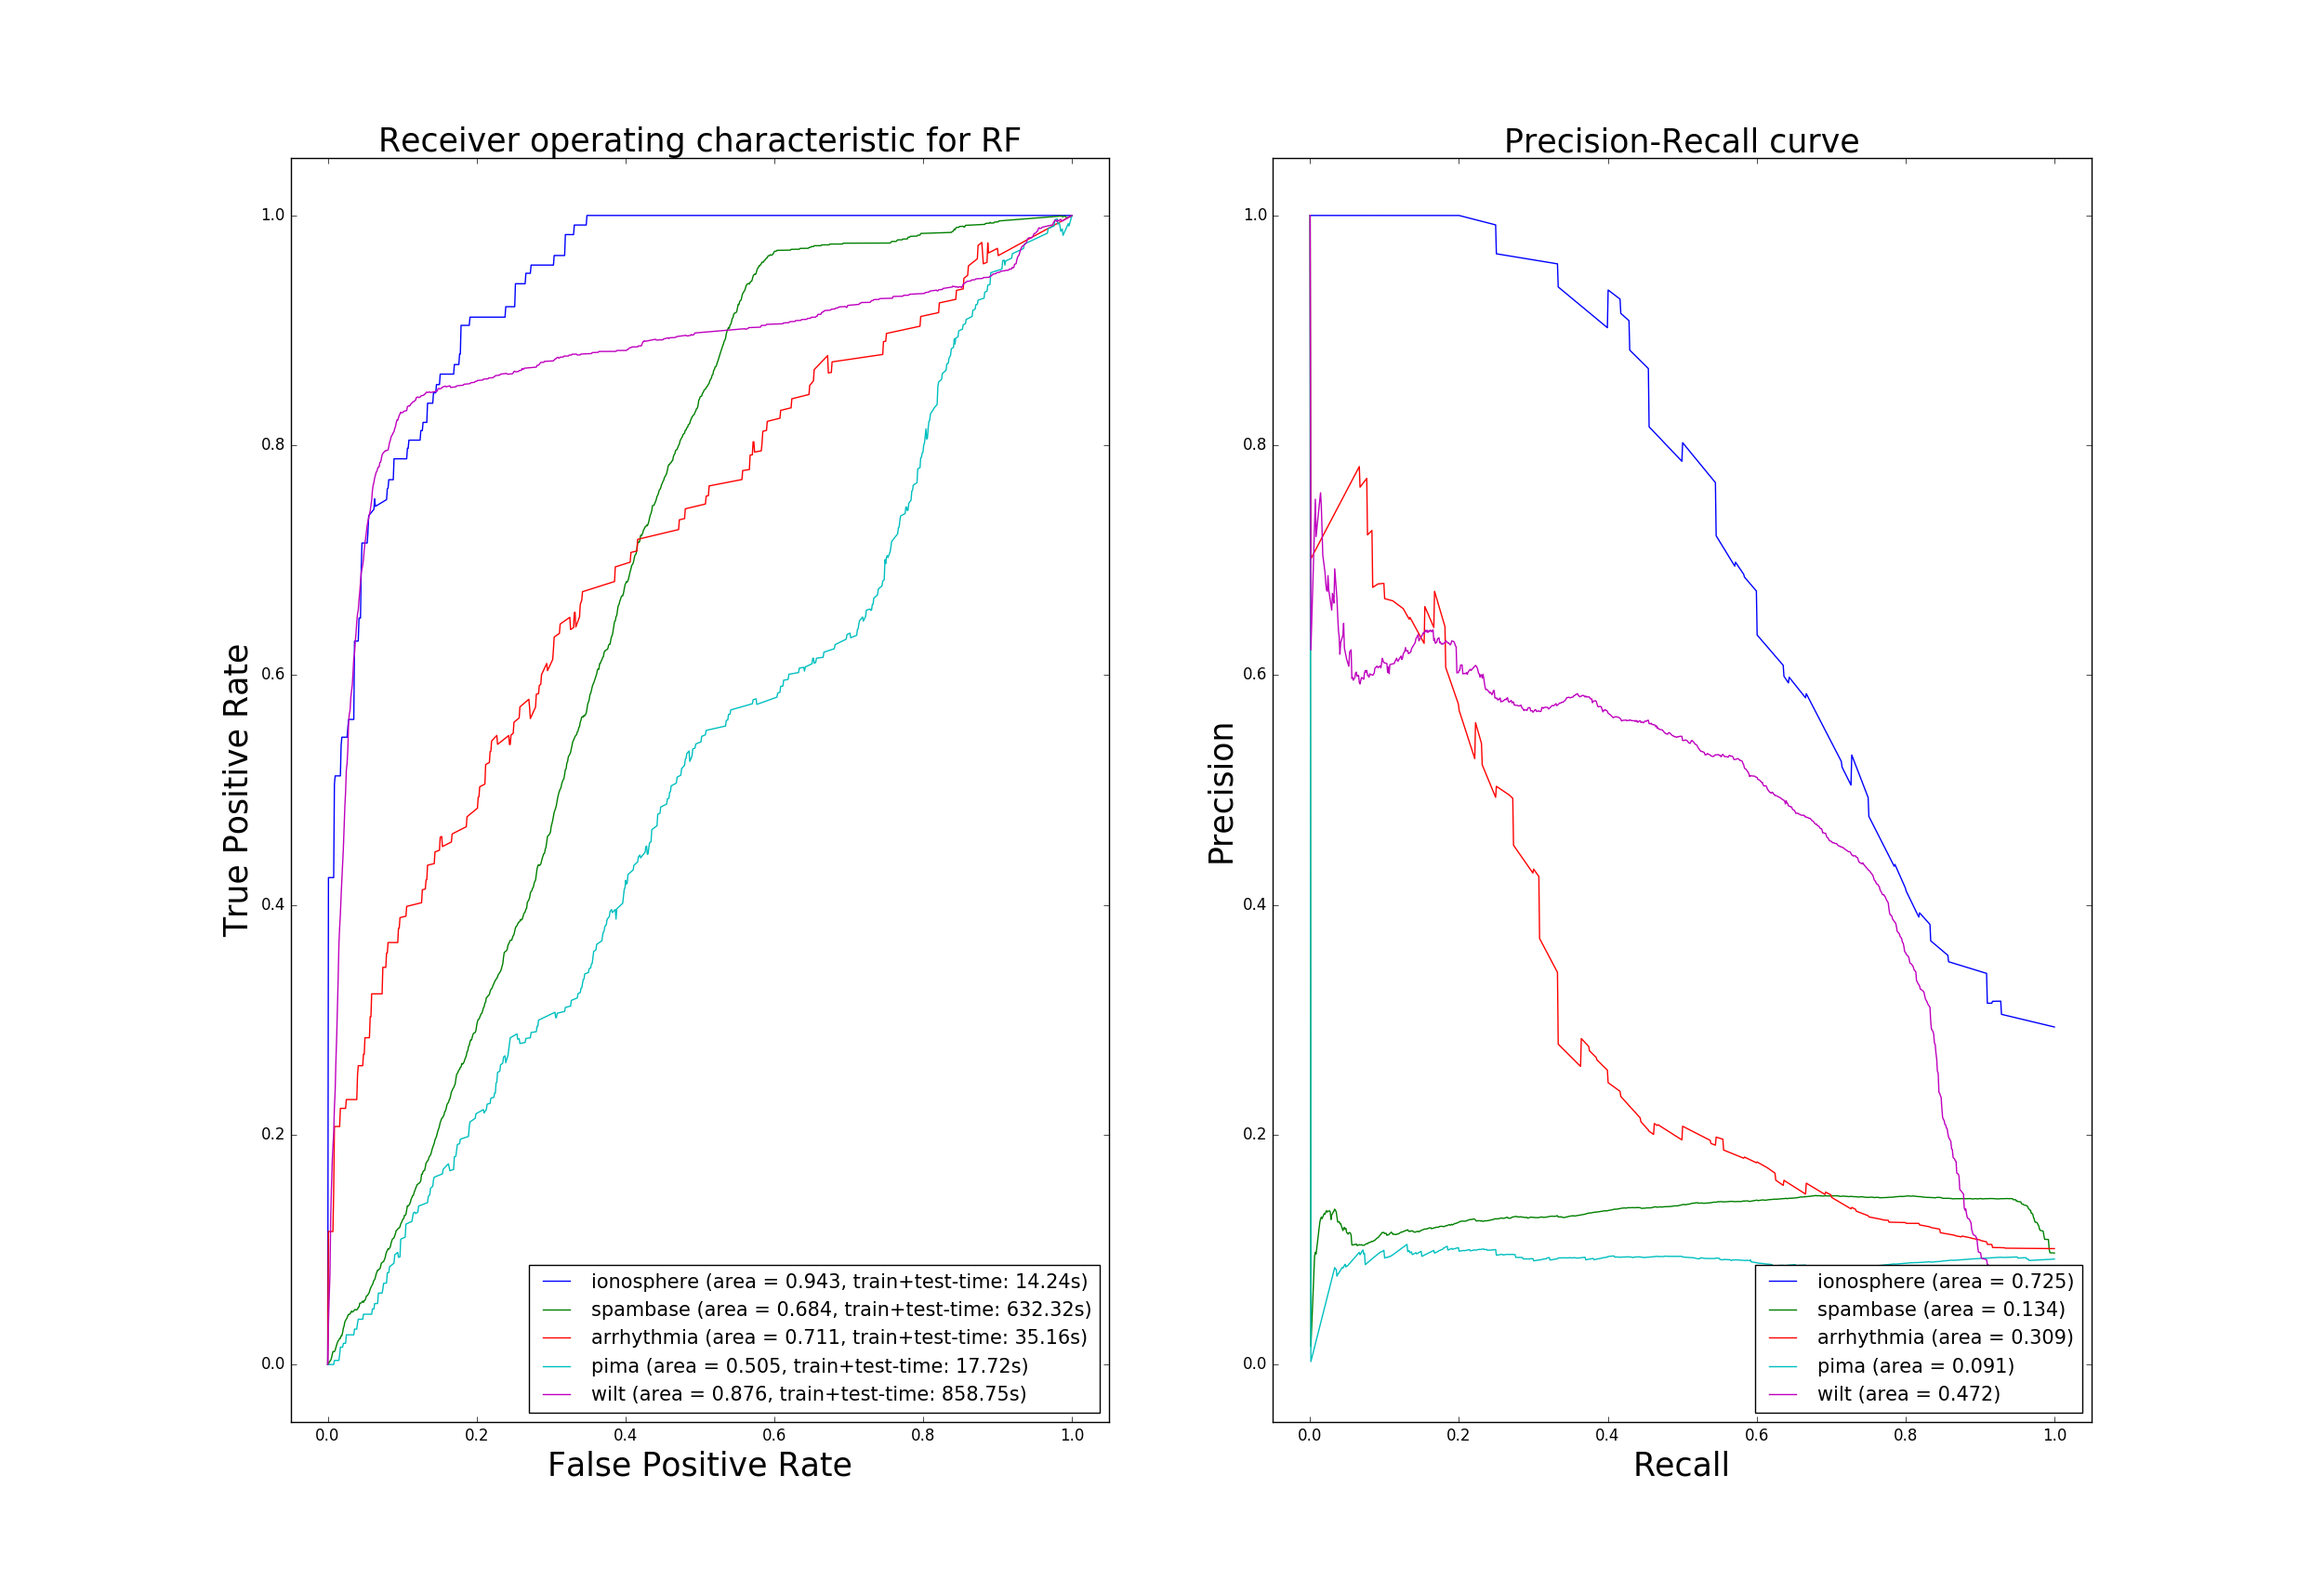
\includegraphics[trim=175 80 175 123, clip, width=\linewidth]{fig_source/ocrf_fig/bench_rf_roc_pr_unsupervised_factorized.png}
\end{figure}





\chapter{Conclusion, limitations \& perspectives}\label{chap:concl}
% \addcontentsline{toc}{chapter}{\nameref{chap:concl}}
% \counterwithout{section}{chapter}
In this thesis, we have addressed three important limitations of existing anomaly detection litterature. The problem of evaluating algorithm in the case of unlabeled data, the problem of extending the use of random forests to one-class classification, and the problem of being accurate on low probability regions.

Our first contribution was to proposed an unsupervised performance criterion, in order to compare scoring functions and to pick one eventually.
%
This excess-mass based criterion resolved some of the drawbacks inherent to the previous mass-volume curve criterion. But the main drawback, estimating a volume in the input space, still remains. This infortunately constitutes a strong setback for its use in a high dimensional framework, if no prior knowledge on the form of these volume to estimate is available. In such a context, classical evaluation approaches must be used, such as ROC or Precision-Recall curves, which assume that at least a small proportion of data is labelled.
Practical unsupervised evaluation criteria still remaining a major challenge (specially under the constraint of scaling with dimension), we studied empirically the use of EM or MV as evaluation criteria and proposed a way to scale their use to high dimensions.

As trying to minimize EM or MV criteria does not produce performant algorithms in practice, we introduced a One Class Random Forest algorithm which structurally extend RFs to one-class classification.
 
Finally, we proposed to focus on extreme regions to gain in accuracy when building scoring functions. An intermediary step was % our fourth contribution, which
to
studies non-asymptotic behavior of an extreme value copula, the stable tail dependence function. We brought new bounds to control the error of its natural empirical version as well as a practical framework for deriving VC-type bounds on low-probability regions.
%
This framework also allows to approach a particular prediction context, namely where the objective is to learn a classifier (or a regressor) that has good properties on low-probability regions.
%
% 
% The previous framework of maximal deviation in low-probability regions also
% opened the road to the statistical ground on which our fifth contribution lies. The latter designs a method that produces a scoring function based on a (possibly sparse) representation of the dependence structure of extremes. Non-asymptotic bounds are derived to assess the accuracy of the estimation procedure, and empirical studies show the relevance of this approach, which is suitable for the treatment of real word large-scale learning problems due to its moderate complexity.
%
Besides, as we exhibit a sparsity pattern in multivariate extremes, it can be used as a preprocessing step to scale up multivariate extreme values modeling to high dimensional settings, which is currently one of the major challenges in multivariate EVT.


%
Staying in the scope of multivariate extremes, the non-asymptotic bounds in the two main results contain separated bias terms corresponding to the (distribution-dependent) convergence speed to the asymptotic behavior, which are not controlled explicitly.
A possible future direction is to make an additional hypothesis
of  `second order regular variation'  \citep[see \emph{e.g.}][]{deHaan1996}
in order to express these bias terms, and possibly to refine the results.
With such explicit bounds, parameters of the Damex algorithm (third contribution) could be chosen optimally as the ones minimizing the obtained bound.

From the scope of one-class random forests, a possible research direction would be to develop theoretical grounds for the level sets estimation procedure. Classical studies from the two-class framework should be adapted to one-class classification.
% As a last contribution (of incremental nature), two classical AD algorithms have been implemented and merged on scikit-learn. They are used in this dissertation for empirical comparison to attest the relevance of the forementionned approach.

% \numberwithin{section}{chapter}

%%\input{ListPublis}
\appendix
%\input{AppendixPR}
%\input{AppendixProofs}
\backmatter
\bibliographystyle{ecs}
\bibliography{Thesis}

\chapter*{Abstract}
\paragraph{Abstract}

% Anomaly, outlier or novelty detection is not only a useful preprocessing step for training machine learning algorithms. It is also a crucial component of lots of real-world applications, from various fields like finance, insurance, telecommunication, computational biology, health or environmental sciences. Anomaly detection is also more and more relevant in the modern world: an increasing number of autonomous systems need to be monitored and diagnosed, specially with the rise of Internet-of-Things.

% Important challenges are



% Learning how to rank multivariate unlabeled observations depending on their degree of abnormality/novelty is a crucial problem in a wide range of applications. In practice, it
% generally consists in building a real valued ”scoring” function on the feature space so as to quantify to which extent observations should be considered as abnormal. 

% In the 1-
% d situation, measurements are generally con-
% sidered as ”abnormal” when they are remote
% from central measures such as the mean or
% the median. Anomaly detection then relies
% on tail analysis of the variable of interest.
% Extensions to the multivariate setting are far
% from straightforward and it is precisely the
% main purpose of this paper to introduce a
% novel and convenient (functional) criterion
% for measuring the performance of a scoring
% function regarding the anomaly ranking task,
% referred to as the Excess-Mass curve (EM
% curve). In addition, an adaptive algorithm
% for building a scoring function based on un-
% labeled data X 1 , . . . , X n with a nearly opti-
% mal EM is proposed and is analyzed from a
% statistical perspective.


% Assessing the probability of occurrence of extreme events is a crucial issue in various fields like
% finance, insurance, telecommunication or environmental sciences. In a multivariate framework, the
% tail dependence is characterized by the so-called stable tail dependence function ( STDF ). Learning
% this structure is the keystone of multivariate extremes. Although extensive studies have proved con-
% sistency and asymptotic normality for the empirical version of the STDF , non-asymptotic bounds
% are still missing. The main purpose of this paper is to fill this gap. Taking advantage of adapted
% VC-type concentration inequalities, upper bounds are derived with expected rate of convergence in
% O(k −1/2 ). The concentration tools involved in this analysis rely on a more general study of max-
% imal deviations in low probability regions, and thus directly apply to the classification of extreme
% data.


% Extremes play a special role in Anomaly Detec-
% tion. Beyond inference and simulation purposes,
% probabilistic tools borrowed from Extreme Value
% Theory (EVT), such as the angular measure, can
% also be used to design novel statistical learning
% methods for Anomaly Detection/ranking. This
% paper proposes a new algorithm based on mul-
% tivariate EVT to learn how to rank observations
% in a high dimensional space with respect to their
% degree of ‘abnormality’. The procedure relies on
% an original dimension-reduction technique in the
% extreme domain that possibly produces a sparse
% representation of multivariate extremes and al-
% lows to gain insight into the dependence struc-
% ture thereof, escaping the curse of dimensional-
% ity. The representation output by the unsuper-
% vised methodology we propose here can be com-
% bined with any Anomaly Detection technique tai-
% lored to non-extreme data. As it performs lin-
% early with the dimension and almost linearly in
% the data (in O(dn log n)), it fits to large scale
% problems. The approach in this paper is novel in
% that EVT has never been used in its multivariate
% version in the field of Anomaly Detection



% Capturing the dependence structure of multivariate extreme events is a major
% concern in many fields involving the management of risks stemming from mul-
% tiple sources, e.g. portfolio monitoring, insurance, environmental risk man-
% agement and anomaly detection. One convenient (nonparametric) charac-
% terization of extreme dependence in the framework of multivariate Extreme
% Value Theory (EVT) is the angular measure, which provides direct informa-
% tion about the probable ’directions’ of extremes, that is, the relative con-
% tribution of each feature/coordinate of the ‘largest’ observations. Modeling
% the angular measure in high dimensional problems is a major challenge for
% the multivariate analysis of rare events. The present paper proposes a novel
% methodology aiming at exhibiting a sparsity pattern within the dependence
% structure of extremes. This is achieved by estimating the amount of mass
% spread by the angular measure on representative sets of directions, corre-
% sponding to specific sub-cones of R d + . This dimension reduction technique
% paves the way towards scaling up existing multivariate EVT methods. Be-
% yond a non-asymptotic study providing a theoretical validity framework for
% our method, we propose as a direct application a –first– Anomaly Detec-
% tion algorithm based on multivariate EVT. This algorithm builds a sparse
% ‘normal profile’ of extreme behaviours, to be confronted with new (possibly
% abnormal) extreme observations. Illustrative experimental results provide
% strong empirical evidence of the relevance of our approach.


% When sufficient labeled data are available, classical criteria based on Receiver
% Operating Characteristic (ROC) or Precision-Recall (PR) curves can be used to
% compare the performance of unsupervised anomaly detection algorithms. However,
% in many situations, few or no data are labeled. This calls for alternative criteria one
% can compute on non-labeled data. In this paper, two criteria that do not require
% labels are empirically shown to discriminate accurately (w.r.t. ROC or PR based
% criteria) between algorithms. These criteria are based on existing Excess-Mass
% (EM) and Mass-Volume (MV) curves, which generally cannot be well estimated in
% large dimension. A methodology based on feature sub-sampling and aggregating is
% also described and tested, extending the use of these criteria to high-dimensional
% datasets and solving major drawbacks inherent to standard EM and MV curves.


% andom Forests (RFs) are strong machine learning tools for classification and
% regression. However, they remain supervised algorithms, and no extension of RFs
% to the one-class setting has been proposed, except for techniques based on second-
% class generation. This paper fills this gap by proposing a natural methodology to
% extend standard splitting criteria to the one-class setting, structurally generalizing
% to one-class classification. Our model is consistent with the two-class framework
% from which our approach can be recovered, considering the asymptotic behavior of
% an adaptive outliers generating process. We also present an extensive benchmark
% of seven state-of-the-art anomaly detection algorithms. This demonstrates the
% empirical relevance of our approach.


\paragraph{Résumé}
\end{document}
%% ----------------------------------------------------------------
